\documentclass[11pt,openany,twoside]{book}
\usepackage[collsonly,ebook]{anthology}
%\documentclass[11pt,letterpaper,openany,twoside]{book}
%\usepackage[collsonly]{anthology}

\begin{document}
\title{An Anthology of Western Philosophy}
\version{2015.06.18}

\frontmatter
\maketitle
\thispagestyle{empty}
\leavevmode\vfil
\begin{center}
\printversion
\vspace{1\baselineskip}

\noindent\parbox{0.7\columnwidth}{\footnotesize All original content in
this collection is in the public domain. All works republished in this
collection are believed to be in the public domain in the United
States. To the extent allowable by law, this collection and its
contents may be copied, reproduced, distributed, or used for
derivative works without permission. All content is presented as is,
without warranty of any kind, either expressed or implied.}

\end{center}
\vfil\vfil\leavevmode
\tableofcontents
\mainmatter


\author{Thucydides}
\authdate{ca. 460 -- ca. 395 \BCE}
\textdate{ca. late 5th, early 4th century \BCE}
\addon[Book 2.34--2.46]{History of the Peloponnesian War}
\chapter{Pericles' Funeral Oration}
\source*{thucydides1900}

\page{125}During the same winter, in accordance with an old national
custom, the funeral of those who first fell in this war was celebrated
by the Athenians at the public charge. The ceremony is as follows:
Three days before the celebration they erect a tent in which the bones
of the dead are laid out, and every one brings to his own dead any
offering which he pleases. At the time of the funeral the bones are
placed in chests of cypress wood, which are conveyed on hearses; there
is one chest for each tribe. They also carry a single empty litter
decked with a pall for all whose bodies are missing, and cannot be
recovered after the battle. The procession is accompanied by any one
who chooses, whether citizen or stranger, and the female relatives of
the deceased are present at the place of interment and make
lamentation. The public sepulchre is situated in the most beautiful
spot outside the walls; there they always bury those who fall in war;
only after the battle of Marathon the dead, in recognition of their
pre-eminent valour, were interred on the field. When the remains have
been laid in the earth, some man of known ability and high reputation,
chosen by the city, delivers a suitable oration over them; after
which the people depart. Such is the manner of interment; and
\page{126} the ceremony was repeated from time to time throughout the
war. Over those who were the first buried Pericles was chosen to
speak. At the fitting moment he advanced from the sepulchre to a lofty
stage, which had been erected in order that he might be heard as far
as possible by the multitude, and spoke as follows:---

\begin{center}\small(FUNERAL SPEECH.)\end{center}

`Most of those who have spoken here before me have commended the
lawgiver who added this oration to our other funeral customs; it
seemed to them a worthy thing that such an honour should be given at
their burial to the dead who have fallen on the field of battle. But I
should have preferred that, when men's deeds have been brave, they
should be honoured in deed only, and with such an honour as this
public funeral, which you are now witnessing. Then the reputation of
many would not have been imperiled on the eloquence or want of
eloquence of one, and their virtues believed or not as he spoke well
or ill. For it is difficult to say neither too little nor too much;
and even moderation is apt not to give the impression of truthfulness.
The friend of the dead who knows the facts is likely to think that the
words of the speaker fall short of his knowledge and of his wishes;
another who is not so well informed, when he hears of anything which
surpasses his own powers, will be envious and will suspect
exaggeration. Mankind are tolerant of the praises of others so long as
each hearer thinks that he can do as well or nearly as well himself,
but, when the speaker rises above him, jealousy is aroused and he
begins to be incredulous. However, since our ancestors have set the
seal of their approval upon the practice, I must obey, and to the
utmost of my power shall endeavour to satisfy the wishes and beliefs
of all who hear me.

\page{127}`I will speak first of our ancestors, for it is right and
seemly that now, when we are lamenting the dead, a tribute should be
paid to their memory. There has never been a time when they did not
inhabit this land, which by their valour they will have handed down
from generation to generation, and we have received from them a free
state. But if they were worthy of praise, still more were our fathers,
who added to their inheritance, and after many a struggle transmitted
to us their sons this great empire. And we ourselves assembled here
to-day, who are still most of us in the vigour of life, have carried
the work of improvement further, and have richly endowed our city with
all things, so that she is sufficient for herself both in peace and
war. Of the military exploits by which our various possessions were
acquired, or of the energy with which we or our fathers drove back the
tide of war, Hellenic or Barbarian, I will not speak; for the tale
would be long and is familiar to you. But before I praise the dead, I
should like to point out by what principles of action we
rose\footnote{Reading \grk{ἤλθομεν}.} to power, and under what
institutions and through what manner of life our empire became great.
For I conceive that such thoughts are not unsuited to the occasion,
and that this numerous assembly of citizens and strangers may
profitably listen to them.

`Our form of government does not enter into rivalry with the
institutions of others. We do not copy our neighbours, but are an
example to them. It is true that we are called a democracy, for the
administration is in the hands of the many and not of the few. But
while there exists equal justice to all and alike in their private
disputes, the claim of excellence is also recognised; and when a
\page{128} citizen is in any way distinguished, he is preferred to the
public service, not as a matter of privilege, but as the reward of
merit. Neither is poverty a bar, but a man may benefit his country
whatever be the obscurity of his condition. There is no exclusiveness
in our public life, and in our private intercourse we are not
suspicious of one another, nor angry with our neighbour if he does
what he likes; we do not put on sour looks at him which, though
harmless, are not pleasant. While we are thus unconstrained in our
private business, a spirit of reverence pervades our public acts; we
are prevented from doing wrong by respect for the authorities and for
the laws, having an especial regard to those which are ordained for
the protection of the injured as well as those unwritten laws which
bring upon the transgressor of them the reprobation of the general
sentiment.

`And we have not forgotten to provide for our weary spirits many
relaxations from toil; we have regular games and sacrifices throughout
the year; our homes are beautiful and elegant; and the delight which
we daily feel in all these things helps to banish melancholy. Because
of the greatness of our city the fruits of the whole earth flow in
upon us; so that we enjoy the goods of other countries as freely as of
our own.

`Then, again, our military training is in many respects superior to
that of our adversaries. Our city is thrown open to the world, and we
never expel a foreigner and prevent him from seeing or learning
anything of which the secret if revealed to an enemy might profit him.
We rely not upon management or trickery, but upon our own hearts and
hands. And in the matter of education, whereas they from early youth
are always undergoing laborious exercises which are to make them
brave, we live at ease, and yet are equally \page{129} ready to face
the perils which they face\footnote{Or, `perils such as our strength
can bear;' or `perils which are enough to daunt us.'}. And here is the
proof. The Lacedaemonians come into Attica not by themselves, but with
their whole confederacy following; we go alone into a neighbour's
country; and although our opponents are fighting for their homes and
we on a foreign soil, we have seldom any difficulty in overcoming
them. Our enemies have never yet felt our united strength; the care of
a navy divides our attention, and on land we are obliged to send our
own citizens everywhere. But they, if they meet and defeat a part of
our army, are as proud as if they had routed us all, and when defeated
they pretend to have been vanquished by us all.

`If then we prefer to meet danger with a light heart but without
laborious training, and with a courage which is gained by habit and
not enforced by law, are we not greatly the gainers? Since we do not
anticipate the pain, although, when the hour comes, we can be as brave
as those who never allow themselves to rest; and thus too our city is
equally admirable in peace and in war. For we are lovers of the
beautiful, yet simple in our tastes, and we cultivate the mind without
loss of manliness. Wealth we employ, not for talk and ostentation, but
when there is a real use for it. To avow poverty with us is no
disgrace; the true disgrace is in doing nothing to avoid it. An
Athenian citizen does not neglect the state because he takes care of
his own household; and even those of us who are engaged in business
have a very fair idea of politics. We alone regard a man who takes no
interest in public affairs, not as a harmless, but as a useless
character; and if few of us are originators, we are all sound judges
of a policy. The great impediment to action \page{130} is, in our
opinion, not discussion, but the want of that knowledge which is
gained by discussion preparatory to action. For we have a peculiar
power of thinking before we act and of acting too, whereas other men
are courageous from ignorance but hesitate upon reflection. And they
are surely to be esteemed the bravest spirits who, having the clearest
sense both of the pains and pleasures of life, do not on that account
shrink from danger. In doing good, again, we are unlike others; we
make our friends by conferring, not by receiving favours. Now he who
confers a favour is the firmer friend, because he would fain by
kindness keep alive the memory of an obligation; but the recipient is
colder in his feelings, because he knows that in requiting another's
generosity he will not be winning gratitude but only paying a debt. We
alone do good to our neighbours not upon a calculation of interest,
but in the confidence of freedom and in a frank and fearless spirit.
To sum up: I say that Athens is the school of Hellas, and that the
individual Athenian in his own person seems to have the power of
adapting himself to the most varied forms of action with the utmost
versatility and grace. This is no passing and idle word, but truth and
fact; and the assertion is verified by the position to which these
qualities have raised the state. For in the hour of trial Athens alone
among her contemporaries is superior to the report of her. No enemy
who comes against her is indignant at the reverses which he sustains
at the hands of such a city; no subject complains that his masters are
unworthy of him. And we shall assuredly not be without witnesses;
there are mighty monuments of our power which will make us the wonder
of this and of succeeding ages; we shall not need the praises of Homer
or of any other panegyrist whose poetry may please for the
moment\footnote{Cp. i. 10 med., and 21.}, \page{131} although his
representation of the facts will not bear the light of day. For we
have compelled every land and every sea to open a path for our valour,
and have everywhere planted eternal memorials of our friendship and of
our enmity. Such is the city for whose sake these men nobly fought and
died; they could not bear the thought that she might be taken from
them; and every one of us who survive should gladly toil on her
behalf.

`I have dwelt upon the greatness of Athens because I want to show you
that we are contending for a higher prize than those who enjoy none of
these privileges, and to establish by manifest proof the merit of
these men whom I am now commemorating. Their loftiest praise has been
already spoken. For in magnifying the city I have magnified them, and
men like them whose virtues made her glorious. And of how few Hellenes
can it be said as of them, that their deeds when weighed in the
balance have been found equal to their fame! Methinks that a death
such as theirs has been the true measure of a man's worth; it may be
the first revelation of his virtues, but is at any rate their final
seal. For even those who come short in other ways may justly plead the
valour with which they have fought for their country; they have
blotted out the evil with the good, and have benefited the state more
by their public services than they have injured her by their private
actions. None of these men were enervated by wealth or hesitated to
resign the pleasures of life; none of them put off the evil day in the
hope, natural to poverty, that a man, though poor, may one day become
rich. But, deeming that the punishment of their enemies was sweeter
than any of these things, and that they could fall in no nobler cause,
they determined at the hazard of their lives to be honorably avenged,
and to leave the rest. They resigned to hope their unknown chance of
happiness; but in the face of death they resolved to rely upon
them-\page{132}selves alone. And when the moment came they were minded
to resist and suffer, rather than to fly and save their lives; they
ran away from the word of dishonour, but on the battle-field their
feet stood fast, and in an instant, at the height of their fortune,
they passed away from the scene, not of their fear, but of their
glory\footnote{Or, taking \grk{τύχης} with \grk{καιροῦ}: `while for a
moment they were in the hands of fortune, at the height, not of terror
but of glory, they passed away.'}.

`Such was the end of these men; they were worthy of Athens, and the
living need not desire to have a more heroic spirit, although they may
pray for a less fatal issue. The value of such a spirit is not to be
expressed in words. Any one can discourse to you for ever about the
advantages of a brave defence, which you know already. But instead of
listening to him I would have you day by day fix your eyes upon the
greatness of Athens, until you become filled with the love of her; and
when you are impressed by the spectacle of her glory, reflect that
this empire has been acquired by men who knew their duty and had the
courage to do it, who in the hour of conflict had the fear of
dishonour always present to them, and who, if ever they failed in an
enterprise, would not allow their virtues to be lost to their country,
but freely gave their lives to her as the fairest offering which they
could present at her feast. The sacrifice which they collectively made
was individually repaid to them; for they received again each one for
himself a praise which grows not old, and the noblest of all
sepulchres---I speak not of that in which their remains are laid, but
of that in which their glory survives, and is proclaimed always and on
every \page{133} fitting occasion both in word and deed. For the whole
earth is the sepulchre of famous men; not only are they commemorated
by columns and inscriptions in their own country, but in foreign lands
there dwells also an unwritten memorial of them, graven not on stone
but in the hearts of men. Make them your examples, and, esteeming
courage to be freedom and freedom to be happiness, do not weigh too
nicely the perils of war. The unfortunate who has no hope of a change
for the better has less reason to throw away his life than the
prosperous who, if he survive, is always liable to a change for the
worse, and to whom any accidental fall makes the most serious
difference. To a man of spirit, cowardice and disaster coming together
are far more bitter than death striking him unperceived at a time when
he is full of courage and animated by the general hope.

`Wherefore I do not now commiserate the parents of the dead who stand
here; I would rather comfort them. You know that your life has been
passed amid manifold vicissitudes; and that they may be deemed
fortunate who have gained most honour, whether an honourable death
like theirs, or an honorable sorrow like yours, and whose days have
been so ordered that the term of their happiness is likewise the term
of their life. I know how hard it is to make you feel this, when the
good fortune of others will too often remind you of the gladness which
once lightened your hearts. And sorrow is felt at the want of those
blessings, not which a man never knew, but which were a part of his
life before they were taken from him. Some of you are of an age at
which they may hope to have other children, and they ought to bear
their sorrow better; not only will the children who may hereafter be
born make them forget their own lost ones, but the city \page{134}
will be doubly a gainer. She will not be left desolate, and she will
be safer. For a man's counsel cannot have equal weight or worth, when
he alone has no children to risk in the general danger. To those of
you who have passed their prime, I say: ``Congratulate yourselves that
you have been happy during the greater part of your days; remember
that your life of sorrow will not last long, and be comforted by the
glory of those who are gone. For the love of honour alone is ever
young, and not riches, as some say, but honour is the delight of men
when they are old and useless.''

`To you who are the sons and brothers of the departed, I see that the
struggle to emulate them will be an arduous one. For all men praise
the dead, and, however preeminent your virtue may be, hardly will you
be thought, I do not say to equal, but even to approach them. The
living have their rivals and detractors, but when a man is out of the
way, the honour and good-will which he receives is unalloyed. And, if
I am to speak of womanly virtues to those of you who will henceforth
be widows, let me sum them up in one short admonition: To a woman not
to show more weakness than is natural to her sex is a great glory, and
not to be talked about for good or for evil among men.

`I have paid the required tribute, in obedience to the law, making use
of such fitting words as I had. The tribute of deeds has been paid in
part; for the dead have been honourably interred, and it remains only
that their children should be maintained at the public charge until
they are grown up: this is the solid prize with which, as with a
garland, Athens crowns her sons living and dead, after a struggle like
theirs. For where the rewards of virtue are greatest, there the
noblest citizens \page{135} are enlisted in the service of the state.
And now, when you have duly lamented, every one his own dead, you may
depart.'

% ca. late 5c., early 4c. BCE

\author{Plato}
\authdate{ca. 427--348/347 \BCE}
\textdate{ca. early fourth century \BCE}
\chapter{Euthyphro}
\source{plato1919.1}

\page{7}\textsc{Euthyphro}. What strange thing has happened, Socrates,
that you have left your accustomed haunts in the Lyceum and are now
haunting the portico where the king archon sits? For it cannot be that
you have an action before the king, as I have.

\textsc{Socrates}. Our Athenians, Euthyphro, do not call it an action,
but an indictment.

\textsc{Euthyphro}. What? Somebody has, it seems, brought an
indictment against you; for I don't accuse you of having brought one
against anyone else.

\textsc{Socrates}. Certainly not.

\textsc{Euthyphro}. But someone else against you?

\textsc{Socrates}. Quite so.

\textsc{Euthyphro}. Who is he?

\textsc{Socrates}. I don't know the man very well myself, Euthyphro,
for he seems to be a young and unknown person. His name, however, is
Meletus, I believe. And he is of the deme of Pitthus, if you remember
any Pitthian Meletus, with long hair and only a little beard, but with
a hooked nose.

\page{9}\textsc{Euthyphro}. I don't remember him, Socrates. But what
sort of an indictment has he brought against you?

\textsc{Socrates}. What sort? No mean one, it seems to me; for the
fact that, young as he is, he has apprehended so important a matter
reflects no small credit upon him. For he says he knows how the youth
are corrupted and who those are who corrupt them. He must be a wise
man; who, seeing my lack of wisdom and that I am corrupting his
fellows, comes to the State, as a boy runs to his mother, to accuse
me. And he seems to me to be the only one of the public men who begins
in the right way; for the right way is to take care of the young men
first, to make them as good as possible, just as a good husbandman
will naturally take care of the young plants first and afterwards of
the rest. And so Meletus, perhaps, is first clearing away us who
corrupt the young plants, as he says; then after this, when he has
turned his attention to the older men, he will bring countless most
precious blessings upon the State,---at least, that is the natural
outcome of the beginning he has made.

\textsc{Euthyphro}. I hope it may be so, Socrates; but I fear the
opposite may result. For it seems to me that he begins by injuring the
State at its very heart, when he undertakes to harm you. Now tell me,
what does he say you do that corrupts the young?

\textsc{Socrates}. Absurd things, my friend, at first hearing. For he
says I am a maker of gods; and because I make new gods and do not
believe in the old ones, he indicted me for the sake of these old
ones, as he says.

\textsc{Euthyphro}. I understand, Socrates; it is because \page{11}
you say the divine monitor keeps coming to you. So he has brought the
indictment against you for making innovations in religion, and he is
going into court to slander you, knowing that slanders on such
subjects are readily accepted by the people. Why, they even laugh at
me and say I am crazy when I say anything in the assembly about divine
things and foretell the future to them. And yet there is not one of
the things I have foretold that is not true; but they are jealous of
all such men as you and I are. However, we must not be disturbed, but
must come to close quarters with them.

\textsc{Socrates}. My dear Euthyphro, their ridicule is perhaps of no
consequence. For the Athenians, I fancy, are not much concerned, if
they think a man is clever, provided he does not impart his clever
notions to others; but when they think he makes others to be like
himself, they are angry with him, either through jealousy, as you say,
or for some other reason.

\textsc{Euthyphro}. I don't much desire to test their sentiments
toward me in this matter.

\textsc{Socrates}. No, for perhaps they think that you are reserved
and unwilling to impart your wisdom. But I fear that because of my
love of men they think that I not only pour myself out copiously to
anyone and everyone without payment, but that I would even pay
something myself, if anyone would listen to me. Now if, as I was
saying just now, they were to laugh at me, as you say they do at you,
it would not be at all unpleasant to pass the time in the court with
jests and laughter; but if they are in earnest, then only soothsayers
like you can tell how this will end.

\page{13}\textsc{Euthyphro}. Well, Socrates, perhaps it won't amount
to much, and you will bring your case to a satisfactory ending, as I
think I shall mine.

\textsc{Socrates}. What is your case, Euthyphro? Are you defending or
prosecuting?

\textsc{Euthyphro}. Prosecuting.

\textsc{Socrates}. Whom?

\textsc{Euthyphro}. Such a man that they think I am insane because I
am prosecuting\footnote{The Greek word has much the same meaning as
the Latin \textit{prosequor}, from which the English `prosecute' is
derived, `follow,' `pursue,' and is at the same time the technical
term for `prosecute.'} him.

\textsc{Socrates}. Why? Are you prosecuting one who has wings to fly
away with?

\textsc{Euthyphro}. No flying for him at his ripe old age.

\textsc{Socrates}. Who is he?

\textsc{Euthyphro}. My father.

\textsc{Socrates}. Your father, my dear man?

\textsc{Euthyphro}. Certainly.

\textsc{Socrates}. But what is the charge, and what is the suit about?

\textsc{Euthyphro}. Murder, Socrates.

\textsc{Socrates}. Heracles! Surely, Euthyphro, most people do not
know where the right lies; for I fancy it is not everyone who can
rightly do what you are doing, but only one who is already very far
advanced in wisdom.

\textsc{Euthyphro}. Very far, indeed, Socrates, by Zeus.

\textsc{Socrates}. Is the one who was killed by your father a
relative? But of course he was; for you would not bring a charge of
murder against him on a stranger's account.

\textsc{Euthyphro}. It is ridiculous, Socrates, that you think it
matters whether the man who was killed \page{15} was a stranger or a
relative, and do not see that the only thing to consider is whether
the action of the slayer was justified or not, and that if it was
justified one ought to let him alone, and if not, one ought to proceed
against him, even if he share one's hearth and eat at one's table. For
the pollution is the same if you associate knowingly with such a man
and do not purify yourself and him by proceeding against him. In this
case, the man who was killed was a hired workman of mine, and when we
were farming at Naxos, he was working there on our land. Now he got
drunk, got angry with one of our house slaves, and butchered him. So
my father bound him hand and foot, threw him into a ditch, and sent a
man here to Athens to ask the religious adviser what he ought to do.
In the meantime he paid no attention to the man as he lay there bound,
and neglected him, thinking that he was a murderer and it did not
matter if he were to die. And that is just what happened to him. For
he died of hunger and cold and his bonds before the messenger came
back from the adviser. Now my father and the rest of my relatives are
angry with me, because for the sake of this murderer I am prosecuting
my father for murder. For they say he did not kill him, and if he had
killed him never so much, yet since the dead man was a murderer, I
ought not to trouble myself about such a fellow, because it is unholy
for a son to prosecute his father for murder. Which shows how little
they know what the divine law is in regard to holiness and unholiness.

\textsc{Socrates}. But, in the name of Zeus, Euthyphro, do you think
your knowledge about divine laws and \page{17} holiness and unholiness
is so exact that, when the facts are as you say, you are not afraid of
doing something unholy yourself in prosecuting your father for murder?

\textsc{Euthyphro}. I should be of no use, Socrates, and Euthyphro
would be in no way different from other men, if I did not have exact
knowledge about all such things.

\textsc{Socrates}. Then the best thing for me, my admirable Euthyphro,
is to become your pupil and, before the suit with Meletus comes on, to
challenge him and say that I always thought it very important before
to know about divine matters and that now, since he says I am doing
wrong by acting carelessly and making innovations in matters of
religion, I have become your pupil. And ``Meletus,'' I should say,
``if you acknowledge that Euthyphro is wise in such matters, then
believe that I also hold correct opinions, and do not bring me to
trial; and if you do not acknowledge that, then bring a suit against
him, my teacher, rather than against me, and charge him with
corrupting the old, namely, his father and me, which he does by
teaching me and by correcting and punishing his father.'' And if he
does not do as I ask and does not release me from the indictment or
bring it against you in my stead, I could say in the court the same
things I said in my challenge to him, could I not?

\textsc{Euthyphro}. By Zeus, Socrates, if he should undertake to
indict me, I fancy I should find his weak spot, and it would be much
more a question about him in court than about me.

\textsc{Socrates}. And I, my dear friend, perceiving this, wish to
become your pupil; for I know that neither \page{19} this fellow
Meletus, nor anyone else, seems to notice you at all, but he has seen
through me so sharply and so easily that he has indicted me for
impiety. Now in the name of Zeus, tell me what you just now asserted
that you knew so well. What do you say is the nature of piety and
impiety, both in relation to murder and to other things? Is not
holiness always the same with itself in every action, and, on the
other hand, is not unholiness the opposite of all holiness, always the
same with itself and whatever is to be unholy possessing some one
characteristic quality?

\textsc{Euthyphro}. Certainly, Socrates.

\textsc{Socrates}. Tell me then, what do you say holiness is, and what
unholiness?

\textsc{Euthyphro}. Well then, I say that holiness is doing what I am
doing now, prosecuting the wrongdoer who commits murder or steals from
the temples or does any such thing, whether he be your father, or your
mother or anyone else, and not prosecuting him is unholy. And,
Socrates, see what a sure proof I offer you,---a proof I have already
given to others,---that this is established and right and that we
ought not to let him who acts impiously go unpunished, no matter who
he may be. Men believe that Zeus is the best and most just of the
gods, and they acknowledge that he put his father in bonds because he
wickedly devoured his children, and he in turn had mutilated his
father for similar reasons; but they are incensed against me because I
proceed against my father when he has done wrong, and so they are
\page{21} inconsistent in what they say about the gods and about me.

\textsc{Socrates}. Is not this, Euthyphro, the reason why I am being
prosecuted, because when people tell such stories about the gods I
find it hard to accept them? And therefore, probably, people will say
I am wrong. Now if you, who know so much about such things, accept
these tales, I suppose I too must give way. For what am I to say, who
confess frankly that I know nothing about them? But tell me, in the
name of Zeus, the god of friendship, do you really believe these
things happened?

\textsc{Euthyphro}. Yes, and still more wonderful things than these,
Soc\-ra\-tes, which most people do not know.

\textsc{Socrates}. And so you believe that there was really war
between the gods, and fearful enmities and battles and other things of
the sort, such as are told of by the poets and represented in varied
designs by the great artists in our sacred places and especially on
the robe which is carried up to the Acropolis at the great
Panathenaea? for this is covered with such representations. Shall we
agree that these things are true, Euthyphro?

\textsc{Euthyphro}. Not only these things, Socrates; but, as I said
just now, I will, if you like, tell you many other things about the
gods, which I am sure will amaze you when you hear them.

\textsc{Socrates}. I dare say. But you can tell me those things at
your leisure some other time. At present try to tell more clearly what
I asked you just now. For, my friend, you did not give me sufficient
information before, when I asked what holiness was, but you told me
that this was holy \page{23} which you are now doing, prosecuting your
father for murder.

\textsc{Euthyphro}. Well, what I said was true, Socrates.

\textsc{Socrates}. Perhaps. But, Euthyphro, you say that many other
things are holy, do you not?

\textsc{Euthyphro}. Why, so they are.

\textsc{Socrates}. Now call to mind that this is not what I asked you,
to tell me one or two of the many holy acts, but to tell the essential
aspect, by which all holy acts are holy; for you said that all unholy
acts were unholy and all holy ones holy by one aspect. Or don't you
remember?

\textsc{Euthyphro}. I remember.

\textsc{Socrates}. Tell me then what this aspect is, that I may keep
my eye fixed upon it and employ it as a model and, if anything you or
anyone else does agrees with it, may say that the act is holy, and if
not, that it is unholy.

\textsc{Euthyphro}. If you wish me to explain in that way, I will do
so.

\textsc{Socrates}. I do wish it.

\textsc{Euthyphro}. Well then, what is dear to the gods is holy, and
what is not dear to them is unholy.

\textsc{Socrates}. Excellent, Euthyphro; now you have answered as I
asked you to answer. However, whether it is true, I am not yet sure;
but you will, of course, show that what you say is true.

\textsc{Euthyphro}. Certainly.

\textsc{Socrates}. Come then, let us examine our words. The thing and
the person that are dear to the gods are holy, and the thing and the
person that are hateful to the gods are unholy; and the two are not
the same, but the holy and the unholy are the \page{25} exact
opposites of each other. Is not this what we have said?

\textsc{Euthyphro}. Yes, just this.

\textsc{Socrates}. And it seems to be correct?

\textsc{Euthyphro}. I think so, Socrates.

\textsc{Socrates}. Well then, have we said this also, that the gods,
Euthyphro, quarrel and disagree with each other, and that there is
enmity between them?

\textsc{Euthyphro}. Yes, we have said that.

\textsc{Socrates}. But what things is the disagreement about, which
causes enmity and anger? Let us look at it in this way. If you and I
were to disagree about number, for instance, which of two numbers were
the greater, would the disagreement about these matters make us
enemies and make us angry with each other, or should we not quickly
settle it by resorting to arithmetic?

\textsc{Euthyphro}. Of course we should.

\textsc{Socrates}. Then, too, if we were to disagree about the
relative size of things, we should quickly put an end to the
disagreement by measuring?

\textsc{Euthyphro}. Yes.

\textsc{Socrates}. And we should, I suppose, come to terms about
relative weights by weighing?

\textsc{Euthyphro}. Of course.

\textsc{Socrates}. But about what would a disagreement be, which we
could not settle and which would cause us to be enemies and be angry
with each other? Perhaps you cannot give an answer offhand; but let
\page{27} me suggest it. Is it not about right and wrong, and noble
and disgraceful, and good and bad? Are not these the questions about
which you and I and other people become enemies, when we do become
enemies, because we differ about them and cannot reach any
satisfactory agreement?

\textsc{Euthyphro}. Yes, Socrates, these are the questions about which
we should become enemies.

\textsc{Socrates}. And how about the gods, Euthyphro? If they
disagree, would they not disagree about these questions?

\textsc{Euthyphro}. Necessarily.

\textsc{Socrates}. Then, my noble Euthyphro, according to what you
say, some of the gods too think some things are right or wrong and
noble or disgraceful, and good or bad, and others disagree; for they
would not quarrel with each other if they did not disagree about these
matters. Is that the case?

\textsc{Euthyphro}. You are right.

\textsc{Socrates}. Then the gods in each group love the things which
they consider good and right and hate the opposites of these things?

\textsc{Euthyphro}. Certainly.

\textsc{Socrates}. But you say that the same things are considered
right by some of them and wrong by others; and it is because they
disagree about these things that they quarrel and wage war with each
other. Is not this what you said?

\textsc{Euthyphro}. It is.

\textsc{Socrates}. Then, as it seems, the same things are hated and
loved by the gods, and the same things would be dear and hateful to
the gods.

\textsc{Euthyphro}. So it seems.

\page{29}\textsc{Socrates}. And then the same things would be both
holy and unholy, Euthyphro, according to this statement.

\textsc{Euthyphro}. I suppose so.

\textsc{Socrates}. Then you did not answer my question, my friend. For
I did not ask you what is at once holy and unholy; but, judging from
your reply, what is dear to the gods is also hateful to the gods. And
so, Euthyphro, it would not be surprising if, in punishing your father
as you are doing, you were performing an act that is pleasing to Zeus,
but hateful to Cronus and Uranus, and pleasing to Hephaestus, but
hateful to Hera, and so forth in respect to the other gods, if any
disagree with any other about it.

\textsc{Euthyphro}. But I think, Socrates, that none of the gods
disagrees with any other about this, or holds that he who kills anyone
wrongfully ought not to pay the penalty.

\textsc{Socrates}. Well, Euthyphro, to return to men, did you ever
hear anybody arguing that he who had killed anyone wrongfully, or had
done anything else whatever wrongfully, ought not to pay the penalty?

\textsc{Euthyphro}. Why, they are always arguing these points,
especially in the law courts. For they do very many wrong things; and
then there is nothing they will not do or say, in defending
themselves, to avoid the penalty.

\textsc{Socrates}. Yes, but do they acknowledge, Euthyphro, that they
have done wrong and, although they acknowledge it, nevertheless say
that they ought not to pay the penalty?

\textsc{Euthyphro}. Oh, no, they don't do that.

\page{31}\textsc{Socrates}. Then there is something they do not do and
say. For they do not, I fancy, dare to say and argue that, if they
have really done wrong, they ought not to pay the penalty; but, I
think, they say they have not done wrong; do they not?

\textsc{Euthyphro}. You are right.

\textsc{Socrates}. Then they do not argue this point, that the
wrongdoer must not pay the penalty; but perhaps they argue about this,
who is a wrongdoer, and what he did, and when.

\textsc{Euthyphro}. That is true.

\textsc{Socrates}. Then is not the same thing true of the gods, if
they quarrel about right and wrong, as you say, and some say others
have done wrong, and some say they have not? For surely, my friend, no
one, either of gods or men, has the face to say that he who does wrong
ought not to pay the penalty.

\textsc{Euthyphro}. Yes, you are right about this, Socrates, in the
main.

\textsc{Socrates}. But I think, Euthyphro, those who dispute, both men
and gods, if the gods do dispute, dispute about each separate act.
When they differ with one another about any act, some say it was right
and others that it was wrong. Is it not so?

\textsc{Euthyphro}. Certainly.

\textsc{Socrates}. Come now, my dear Euthyphro, inform me, that I may
be made wiser, what proof you have that all the gods think that the
man lost his life wrongfully, who, when he was a servant, committed
\page{33} murder, was bound by the master of the man he killed, and
died as a result of his bonds before the master who had bound him
found out from the advisers what he ought to do with him, and that it
is right on account of such a man for a son to proceed against his
father and accuse him of murder. Come, try to show me clearly about
this, that the gods surely believe that this conduct is right; and if
you show it to my satisfaction, I will glorify your wisdom as long as
I live.

\textsc{Euthyphro}. But perhaps this is no small task, Socrates;
though I could show you quite clearly.

\textsc{Socrates}. I understand; it is because you think I am slower
to understand than the judges; since it is plain that you will show
them that such acts are wrong and that all the gods hate them.

\textsc{Euthyphro}. Quite clearly, Socrates; that is, if they listen
to me.

\textsc{Socrates}. They will listen, if they find that you are a good
speaker. But this occurred to me while you were talking, and I said to
myself: ``If Euthyphro should prove to me no matter how clearly that
all the gods think such a death is wrongful, what have I learned from
Euthyphro about the question, what is holiness and what is unholiness?
For this act would, as it seems, be hateful to the gods; but we saw
just now that holiness and its opposite are not defined in this way;
for we saw that what is hateful to the gods is also dear to them; and
so I let you off any discussion of this point, Euthyphro. If you like,
all the gods may think it wrong and may hate it. But shall we now
emend our definition and \page{35} say that whatever all the gods hate
is unholy and whatever they all love is holy, and what some love and
others hate is neither or both? Do you wish this now to be our
definition of holiness and unholiness?

\textsc{Euthyphro}. What is to hinder, Socrates?

\textsc{Socrates}. Nothing, so far as I am concerned, Euthyphro, but
consider your own position, whether by adopting this definition you
will most easily teach me what you promised.

\textsc{Euthyphro}. Well, I should say that what all the gods love is
holy and, on the other hand, what they all hate is unholy.

\textsc{Socrates}. Then shall we examine this again, Euthyphro, to see
if it is correct, or shall we let it go and accept our own statement,
and those of others, agreeing that it is so, if anyone merely says
that it is? Or ought we to inquire into the correctness of the
statement?

\textsc{Euthyphro}. We ought to inquire. However, I think this is now
correct.

\textsc{Socrates}. We shall soon know more about this, my friend. Just
consider this question:---Is that which is holy loved by the gods
because it is holy, or is it holy because it is loved by the gods?

\textsc{Euthyphro}. I don't know what you mean, Socrates.

\textsc{Socrates}. Then I will try to speak more clearly. We speak of
being carried and of carrying, of being led and of leading, of being
seen and of seeing; and you understand---do you not?---that in all
such expressions the two parts differ one from the other in meaning,
and how they differ.

\textsc{Euthyphro}. I think I understand.

\page{37}\textsc{Socrates}. Then, too, we conceive of a thing being
loved and of a thing loving, and the two are different?

\textsc{Euthyphro}. Of course.

\textsc{Socrates}. Now tell me, is a thing which is carried a carried
thing because one carries it, or for some other reason?

\textsc{Euthyphro}. No, for that reason.

\textsc{Socrates}. And a thing which is led is led because one leads
it, and a thing which is seen is so because one sees it?

\textsc{Euthyphro}. Certainly.

\textsc{Socrates}. Then one does not see it because its a seen thing,
but, on the contrary, it is a seen thing because one sees it; and one
does not lead it because it is a led thing, but it is a led thing
because one leads it; and one does not carry it because it is a
carried thing, but it is a carried thing because one carries it. Is it
clear, Euthyphro, what I am trying to say? I am trying to say this,
that if anything becomes or undergoes, it does not become because it
is in a state of becoming, but it is in a state of becoming because it
becomes, and it does not undergo because it is a thing which
undergoes, but because it undergoes it is a thing which undergoes; or
do you not agree to this?

\textsc{Euthyphro}. I agree.

\textsc{Socrates}. Is not that which is beloved a thing which is
either becoming or undergoing something?

\textsc{Euthyphro}. Certainly.

\textsc{Socrates}. And is this case like the former ones: those who
love it do not love it because it is a beloved thing, but it is a
beloved thing because they love it?

\textsc{Euthyphro}. Obviously.

\page{39}\textsc{Socrates}. Now what do you say about that which is
holy, Euthyphro? It is loved by all the gods, is it not, according to
what you said?

\textsc{Euthyphro}. Yes.

\textsc{Socrates}. For this reason, because it is holy, or for some
other reason?

\textsc{Euthyphro}. No, for this reason.

\textsc{Socrates}. It is loved because it is holy, not holy because it
is loved?

\textsc{Euthyphro}. I think so.

\textsc{Socrates}. But that which is dear to the gods is dear to them
and beloved by them because they love it.

\textsc{Euthyphro}. Of course.

\textsc{Socrates}. Then that which is dear to the gods and that which
is holy are not identical, but differ one from the other.

\textsc{Euthyphro}. How so, Socrates?

\textsc{Socrates}. Because we are agreed that the holy is loved
because it is holy and that it is not holy because it is loved; are we
not?

\textsc{Euthyphro}. Yes.

\textsc{Socrates}. But we are agreed that what is dear to the gods is
dear to them because they love it, that is, by reason of this love,
not that they love it because it is dear.

\textsc{Euthyphro}. Very true.

\textsc{Socrates}. But if that which is dear to the gods and that
which is holy were identical, my dear Euthyphro, then if the holy were
loved because it is holy, that which is dear to the gods would be
loved because it is dear, and if that which is dear to the gods is
dear because it is loved, then that which is holy would be holy
because \page{41} it is loved; but now you see that the opposite is
the case, showing that the two are different from each other. For the
one becomes lovable from the fact that it is loved, whereas the other
is loved because it is in itself lovable. And, Euthyphro, it seems
that when you were asked what holiness is you were unwilling to make
plain its essence, but you mentioned something that has happened to
this holiness, namely, that it is loved by the gods. But you did not
tell as yet what it really is. So, if you please, do not hide it from
me, but begin over again and tell me what holiness is, no matter
whether it is loved by the gods or anything else happens it; for we
shall not quarrel about that. But tell me frankly, What is holiness,
and what is unholiness?

\textsc{Euthyphro}. But, Socrates, I do not know how to say what I
mean. For whatever statement we advance, somehow or other it moves
about and won't stay where we put it.

\textsc{Socrates}. Your statements, Euthyphro, are like works of
my\footnote{Socrates was the son of a sculptor and was himself
educated to be a sculptor. This is doubtless the reason for his
reference to Daedalus as an ancestor. Daedalus was a half mythical
personage whose statues were said to have been so lifelike that they
moved their eyes and walked about.} ancestor Daedalus, and if I were
the one who made or advanced them, you might laugh at me and say that
on account of my relationship to him my works in words run away and
won't stay where they are put. But now---well, the statements are
yours; so some other jest is demanded; for they stay fixed, as you
yourself see.

\textsc{Euthyphro}. I think the jest does very well as it \page{43}
is; for I am not the one who makes these statements move about and not
stay in the same place, but you are the Daedalus; for they would have
stayed, so far as I am concerned.

\textsc{Socrates}. Apparently then, my friend, I am a more clever
artist than Daedalus, inasmuch as he made only his own works move,
whereas I, as it seems, give motion to the works of others as well as
to my own. And the most exquisite thing about my art is that I am
clever against my will; for I would rather have my words stay fixed
and stable than possess the wisdom of Daedalus and the wealth of
Tantalus besides. But enough of this. Since you seem to be indolent, I
will aid you myself, so that you may instruct me about holiness. And
do not give it up beforehand. Just see whether you do not think that
everything that is holy is right.

\textsc{Euthyphro}. I do.

\textsc{Socrates}. But is everything that is right also holy? Or is
all which is holy right, and not all which is right holy, but part of
it holy and part something else?

\textsc{Euthyphro}. I can't follow you, Socrates.

\textsc{Socrates}. And yet you are as much younger than I as you are
wiser; but, as I said, you are indolent on account of your wealth of
wisdom. But exert \page{45} yourself, my friend; for it is not hard to
understand what I mean. What I mean is the opposite of what the
poet\footnote{Stasinus, author of the ``Cypria'' (Fragm. 20, ed.
Kinkel).} said, who wrote: ``Zeus the creator, him who made all
things, thou wilt not name; for where fear is, there also is
reverence.'' Now I disagree with the poet. Shall I tell you how?

\textsc{Euthyphro}. By all means.

\textsc{Socrates}. It does not seem to me true that where fear is,
there also is reverence; for many who fear diseases and poverty and
other such things seem to me to fear, but not to reverence at all
these things which they fear. Don't you think so, too?

\textsc{Euthyphro}. Certainly.

\textsc{Socrates}. But I think that where reverence is, there also is
fear; for does not everyone who has a feeling of reverence and shame
about any act also dread and fear the reputation for wickedness?

\textsc{Euthyphro}. Yes, he does fear.

\textsc{Socrates}. Then it is not correct to say ``where fear is,
there also is reverence.'' On the contrary, where reverence is, there
also is fear; but reverence is not everywhere where fear is, since, as
I think, fear is more comprehensive than reverence; for reverence is a
part of fear, just as the odd is a part of number, so that it is not
true that where number is, there also is the odd, but that where the
odd is, there also is number. Perhaps you follow me now?

\textsc{Euthyphro}. Perfectly.

\textsc{Socrates}. It was something of this sort that I meant before,
when I asked whether where the right is, there also is holiness, or
where holiness is, \page{47} there also is the right; but holiness is
not everywhere where the right is, for holiness is a part of the
right. Do we agree to this, or do you dissent?

\textsc{Euthyphro}. No, I agree; for I think the statement is correct.

\textsc{Socrates}. Now observe the next point. If holiness is a part
of the right, we must, apparently, find out what part of the right
holiness is. Now if you asked me about one of the things I just
mentioned, as, for example, what part of number the even was, and what
kind of a number it was I should say, ``that which is not indivisible
by two, but divisible by two''; or don't you agree?

\textsc{Euthyphro}. I agree.

\textsc{Socrates}. Now try in your turn to teach me what part of the
right holiness is, that I may tell Meletus not to wrong me any more or
bring suits against me for impiety, since I have now been duly
instructed by you about what is, and what is not, pious and holy.

\textsc{Euthyphro}. This then is my opinion, Socrates, that the part
of the right which has to do with attention to the gods constitutes
piety and holiness, and that the remaining part of the right is that
which has to do with the service of men.

\textsc{Socrates}. I think you are correct, Euthyphro; but there is
one little point about which I still want information, for I do not
yet understand what you mean by ``attention.'' I don't suppose you
mean the same kind of attention to the gods which is paid to other
things. We say, for example, that not everyone knows how to attend to
horses, but only he who is skilled in horsemanship, do we not?

\page{49}\textsc{Euthyphro}. Certainly.

\textsc{Socrates}. Then horsemanship is the art of attending to
horses?

\textsc{Euthyphro}. Yes.

\textsc{Socrates}. And not everyone knows how to attend to dogs, but
only the huntsman?

\textsc{Euthyphro}. That is so.

\textsc{Socrates}. Then the huntsman's art is the art of attending to
dogs?

\textsc{Euthyphro}. Yes.

\textsc{Socrates}. And the oxherd's art is that of attending to oxen?

\textsc{Euthyphro}. Certainly.

\textsc{Socrates}. And holiness and piety is the art of attending to
the gods? Is that what you mean, Euthyphro?

\textsc{Euthyphro}. Yes.

\textsc{Socrates}. Now does attention always aim to accomplish the
same end? I mean something like this: It aims at some good or benefit
to the one to whom it is given, as you see that horses, when attended
to by the horseman's art are benefited and made better; or don't you
think so?

\textsc{Euthyphro}. Yes, I do.

\textsc{Socrates}. And dogs are benefited by the huntsman's art and
oxen by the oxherd's and everything else in the same way? Or do you
think care and attention are ever meant for the injury of that which
is cared for?

\textsc{Euthyphro}. No, by Zeus, I do not.

\textsc{Socrates}. But for its benefit?

\textsc{Euthyphro}. Of course.

\textsc{Socrates}. Then holiness, since it is the art of attending to
the gods, is a benefit to the gods, and \page{51} makes them better?
And you would agree that when you do a holy or pious act you are
making one of the gods better?

\textsc{Euthyphro}. No, by Zeus, not I.

\textsc{Socrates}. Nor do I, Euthyphro, think that is what you meant.
Far from it. But I asked what you meant by ``attention to the gods''
just because I did not think you meant anything like that.

\textsc{Euthyphro}. You are right, Socrates; that is not what I mean.

\textsc{Socrates}. Well, what kind of attention to the gods is
holiness?

\textsc{Euthyphro}. The kind, Socrates, that servants pay to their
masters.

\textsc{Socrates}. I understand. It is, you mean, a kind of service to
the gods?

\textsc{Euthyphro}. Exactly.

\textsc{Socrates}. Now can you tell me what result the art that serves
the physician serves to produce? Is it not health?

\textsc{Euthyphro}. Yes.

\textsc{Socrates}. Well then; what is it which the art that serves
shipbuilders serves to produce?

\textsc{Euthyphro}. Evidently, Socrates, a ship.

\textsc{Socrates}. And that which serves housebuilders serves to build
a house?

\textsc{Euthyphro}. Yes.

\textsc{Socrates}. Then tell me, my friend; what would the art which
serves the gods serve to accomplish? For it is evident that you know,
since you say you know more than any other man about matters which
have to do with the gods.

\textsc{Euthyphro}. And what I say is true, Socrates.

\textsc{Socrates}. Then, in the name of Zeus, tell me, \page{53} what
is that glorious result which the gods accomplish by using us as
servants?

\textsc{Euthyphro}. They accomplish many fine results, Socrates.

\textsc{Socrates}. Yes, and so do generals, my friend; but
nevertheless, you could easily tell the chief of them, namely, that
they bring about victory in war. Is that not the case?

\textsc{Euthyphro}. Of course.

\textsc{Socrates}. And farmers also, I think, accomplish many fine
results; but still the chief result of their work is food from the
land?

\textsc{Euthyphro}. Certainly.

\textsc{Socrates}. But how about the many fine results the gods
accomplish? What is the chief result of their work?

\textsc{Euthyphro}. I told you a while ago, Socrates, that it is a
long task to learn accurately all about these things. However, I say
simply that when one knows how to say and do what is gratifying to the
gods, in praying and sacrificing, that is holiness, and such things
bring salvation to individual families and to states; and the opposite
of what is gratifying to the gods is impious, and that overturns and
destroys everything.

% NOTE: added missing comma after 'Euthyphro'

\textsc{Socrates}. You might, if you wished, Euthyphro, have answered
much more briefly the chief part of my question. But it is plain that
you do not care to instruct me. For now, when you were close upon it
you turned aside; and if you had answered it, I should already have
obtained from you all the instruction I need about holiness. But, as
things are, the questioner must follow the one questioned wherever he
leads. What do you say the holy, or \page{55} holiness, is? Do you not
say that it is a kind of science of sacrificing and praying?

\textsc{Euthyphro}. Yes.

\textsc{Socrates}. And sacrificing is making gifts to the gods and
praying is asking from them?

\textsc{Euthyphro}. Exactly, Socrates.

\textsc{Socrates}. Then holiness, according to this definition, would
be a science of giving and asking.

\textsc{Euthyphro}. You understand perfectly what I said, Socrates.

\textsc{Socrates}. Yes, my friend, for I am eager for your wisdom, and
give my mind to it, so that nothing you say shall fall to the ground.
But tell me, what is this service of the gods? Do you say that it
consists in asking from them and giving to them?

\textsc{Euthyphro}. Yes.

\textsc{Socrates}. Would not the right way of asking be to ask of them
what we need from them?

\textsc{Euthyphro}. What else?

\textsc{Socrates}. And the right way of giving, to present them with
what they need from us? For it would not be scientific giving to give
anyone what he does not need.

\textsc{Euthyphro}. You are right, Socrates.

\textsc{Socrates}. Then holiness would be an art of barter between
gods and men?

\textsc{Euthyphro}. Yes, of barter, if you like to call it so.

\textsc{Socrates}. I don't like to call it so, if it is not true. But
tell me, what advantage accrues to the gods from \page{57} the gifts
they get from us? For everybody knows what they give, since we have
nothing good which they do not give. But what advantage do they derive
from what they get from us? Or have we so much the better of them in
our bartering that we get all good things from them and they nothing
from us?

\textsc{Euthyphro}. Why you don't suppose, Socrates, that the gods
gain any advantage from what they get from us, do you?

\textsc{Socrates}. Well then, what would those gifts of ours to the
gods be?

\textsc{Euthyphro}. What else than honour and praise, and, as I said
before, gratitude?

\textsc{Socrates}. Then, Euthyphro, holiness is grateful to the gods,
but not advantageous or precious to the gods?

\textsc{Euthyphro}. I think it is precious, above all things.

\textsc{Socrates}. Then again, it seems, holiness is that which is
precious to the gods.

\textsc{Euthyphro}. Certainly.

\textsc{Socrates}. Then will you be surprised, since you say this, if
your words do not remain fixed but walk about, and will you accuse me
of being the Daedalus who makes them walk, when you are yourself much
more skilful than Daedalus and make them go round in a circle? Or do
you not see that our definition has come round to the point from which
it started? For you remember, I suppose, that a while ago we found
that holiness and what is dear to the gods were not the same, but
different from each other; or do you not remember?

\textsc{Euthyphro}. Yes, I remember.

\textsc{Socrates}. Then don't you see that now you say \page{59} that
what is precious to the gods is holy? And is not this what is dear to
the gods?

\textsc{Euthyphro}. Certainly.

\textsc{Socrates}. Then either our agreement a while ago was wrong, or
if that was right, we are wrong now.

\textsc{Euthyphro}. So it seems.

\textsc{Socrates}. Then we must begin again at the beginning and ask
what holiness is. Since I shall not willingly give up until I learn.
And do not scorn me, but by all means apply your mind now to the
utmost and tell me the truth; for you know, if anyone does, and like
Proteus, you must be held until you speak. For if you had not clear
knowledge of holiness and unholiness, you would surely not have
undertaken to prosecute your aged father for murder for the sake of a
servant. You would have been afraid to risk the anger of the gods, in
case your conduct should be wrong, and would have been ashamed in the
sight of men. But now I am sure you think you know what is holy and
what is not. So tell me, most excellent Euthyphro, and do not conceal
your thought.

\textsc{Euthyphro}. Some other time, Socrates. Now I am in a hurry and
it is time for me to go.

\textsc{Socrates}. Oh my friend, what are you doing? You go away and
leave me cast down from the high hope I had that I should learn from
you what is holy, and what is not, and should get rid of Meletus's
indictment by showing him that I have been made wise by Euthyphro
about divine matters and am no longer through ignorance acting
carelessly and making innovations in respect to them, and that I shall
live a better life henceforth.

% ca. early 4c. BCE

\author{Plato}
\authdate{ca. 427--348/347 {\smaller BCE}}
%\textdate{ca. 380}
\chapter[Plato -- Glaucon on the Ring of Gyges]{Glaucon on the Ring of
Gyges\\\smaller Republic\\\smaller Book 2, 358e--60d}

%\nfootnote{\fullcite*[bk 2, 358e--60d]{plato1908.1}}
\nfootnote{\fullcite*{plato1908.1}}

% No page numbers in cited text, only Stephanus numbers. There's no
% precise way to insert them, however, since the line breaks here are
% different.

They say that to do injustice is, by nature, good; to suffer
injustice, evil; but that the evil is greater than the good. And so
when men have both done and suffered injustice and have had experience
of both, not being able to avoid the one and obtain the other, they
think that they had better agree among themselves to have neither;
hence there arise laws and mutual covenants; and that which is
ordained by law is termed by them lawful and just. This they affirm to
be the origin and nature of jus\-tice;---it is a mean or compromise,
between the best of all, which is to do injustice and not be punished,
and the worst of all, which is to suffer injustice without the power
of retaliation; and justice, being at a middle point between the two,
is tolerated not as a good, but as the lesser evil, and honoured by
reason of the inability of men to do injustice. For no man who is
worthy to be called a man would ever submit to such an agreement if he
were able to resist; he would be mad if he did. Such is the received
account, Socrates, of the nature and origin of justice.

Now that those who practise justice do so involuntarily and because
they have not the power to be unjust will best appear if we imagine
something of this kind: having given both to the just and the unjust
power to do what they will, let us watch and see whither desire will
lead them; then we shall discover in the very act the just and unjust
man to be proceeding along the same road, following their interest,
which all natures deem to be their good, and are only diverted into
the path of justice by the force of law. The liberty which we are
supposing may be most completely given to them in the form of such a
power as is said to have been possessed by Gyges, the ancestor of
Croesus the Lydian. According to the tradition, Gyges was a shepherd
in the service of the king of Lydia; there was a great storm, and an
earthquake made an opening in the earth at the place where he was
feeding his flock. Amazed at the sight, he descended into the opening,
where, among other marvels, he beheld a hollow brazen horse, having
doors, at which he stooping and looking in saw a dead body of stature,
as appeared to him, more than human, and having nothing on but a gold
ring; this he took from the finger of the dead and reascended. Now the
shepherds met together, according to custom, that they might send
their monthly report about the flocks to the king; into their assembly
he came having the ring on his finger, and as he was sitting among
them he chanced to turn the collet of the ring inside his hand, when
instantly he became invisible to the rest of the company and they
began to speak of him as if he were no longer present. He was
astonished at this, and again touching the ring he turned the collet
outwards and reappeared; he made several trials of the ring, and
always with the same result---when he turned the collet inwards he
became invisible, when outwards he reappeared. Whereupon he contrived
to be chosen one of the messengers who were sent to the court; where
as soon as he arrived he seduced the queen, and with her help
conspired against the king and slew him, and took the kingdom. Suppose
now that there were two such magic rings, and the just put on one of
them and the unjust the other; no man can be imagined to be of such an
iron nature that he would stand fast in justice. No man would keep his
hands off what was not his own when he could safely take what he liked
out of the market, or go into houses and lie with any one at his
pleasure, or kill or release from prison whom he would, and in all
respects be like a god among men. Then the actions of the just would
be as the actions of the unjust; they would both come at last to the
same point. And this we may truly affirm to be a great proof that a
man is just, not willingly or because he thinks that justice is any
good to him individually, but of necessity, for wherever any one
thinks that he can safely be unjust, there he is unjust. For all men
believe in their hearts that injustice is far more profitable to the
individual than justice, and he who argues as I have been supposing,
will say that they are right. If you could imagine any one obtaining
this power of becoming invisible, and never doing any wrong or
touching what was another's, he would be thought by the lookers-on to
be a most wretched idiot, although they would praise him to one
another's faces, and keep up appearances with one another from a fear
that they too might suffer injustice.

% ca. 380?

\author{Plato}
\authdate{ca. 427--348/347 \BCE}
%\textdate{ca. 380 \BCE}
\textdate{ca. early fourth century \BCE}
\addon[Book 7, 514a--19b]{Republic}
\chapter{Socrates' Allegory of the Cave}
%\source*[bk 7, 514a--19b]{plato1908.2}
\source*{plato1908.2}

% No page numbers in cited text, only Stephanus numbers. However,
% there's no precise way to insert the Stephanus numbers, since the
% line breaks here are different.

And now, I said, let me show in a figure how far our nature is
enlightened or un\-en\-light\-ened:---Behold! human beings living in
an underground den, which has a mouth open towards the light and
reaching all along the den; here they have been from their childhood,
and have their legs and necks chained so that they cannot move, and
can only see before them, being prevented by the chains from turning
round their heads. Above and behind them a fire is blazing at a
distance, and between the fire and the prisoners there is a raised
way; and you will see, if you look, a low wall built along the way,
like the screen which marionette players have in front of them, over
which they show the puppets.

I see.

And do you see, I said, men passing along the wall carrying all sorts
of vessels, and statues and figures of animals made of wood and stone
and various materials, which appear over the wall? Some of them are
talking, others silent.

You have shown me a strange image, and they are strange prisoners.

Like ourselves, I replied; and they see only their own shadows, or the
shadows of one another, which the fire throws on the opposite wall of
the cave?

True, he said; how could they see anything but the shadows if they
were never allowed to move their heads?

And of the objects which are being carried in like manner they would
only see the shadows?

Yes, he said.

And if they were able to converse with one another, would they not
suppose that they were naming what was actually before them?

Very true.

And suppose further that the prison had an echo which came from the
other side, would they not be sure to fancy when one of the passers-by
spoke that the voice which they heard came from the passing shadow?

No question, he replied.

To them, I said, the truth would be literally nothing but the shadows
of the images.

That is certain.

And now look again, and see what will naturally follow if the
prisoners are released and disabused of their error. At first, when
any of them is liberated and compelled suddenly to stand up and turn
his neck round and walk and look towards the light, he will suffer
sharp pains; the glare will distress him, and he will be unable to see
the realities of which in his former state he had seen the shadows;
and then conceive some one saying to him, that what he saw before was
an illusion, but that now, when he is approaching nearer to being and
his eye is turned towards more real existence, he has a clearer
vi\-sion,---what will be his reply? And you may further imagine that
his instructor is pointing to the objects as they pass and requiring
him to name them,---will he not be perplexed? Will he not fancy that
the shadows which he formerly saw are truer than the objects which are
now shown to him?

Far truer.

And if he is compelled to look straight at the light, will he not have
a pain in his eyes which will make him turn away to take refuge in the
objects of vision which he can see, and which he will conceive to be
in reality clearer than the things which are now being shown to him?

True, he said.

And suppose once more, that he is reluctantly dragged up a steep and
rugged ascent, and held fast until he is forced into the presence of
the sun himself, is he not likely to be pained and irritated? When he
approaches the light his eyes will be dazzled, and he will not be able
to see anything at all of what are now called realities.

Not all in a moment, he said.

He will require to grow accustomed to the sight of the upper world.
And first he will see the shadows best, next the reflections of men
and other objects in the water, and then the objects themselves; then
he will gaze upon the light of the moon and the stars and the spangled
heaven; and he will see the sky and the stars by night better than the
sun or the light of the sun by day?

Certainly.

Last of all he will be able to see the sun, and not mere reflections
of him in the water, but he will see him in his own proper place, and
not in another; and he will contemplate him as he is.

Certainly.

He will then proceed to argue that this is he who gives the season and
the years, and is the guardian of all that is in the visible world,
and in a certain way the cause of all things which he and his fellows
have been accustomed to behold?

Clearly, he said, he would first see the sun and then reason about
him.

And when he remembered his old habitation, and the wisdom of the den
and his fellow-prisoners, do you not suppose that he would felicitate
himself on the change, and pity him?

Certainly, he would.

And if they were in the habit of conferring honours among themselves
on those who were quickest to observe the passing shadows and to
remark which of them went before, and which followed after, and which
were together; and who were therefore best able to draw conclusions as
to the future, do you think that he would care for such honours and
glories, or envy the possessors of them? Would he not say with Homer,

\begin{quote} Better to be the poor servant of a poor master,
\end{quote}

\noindent and to endure anything, rather than think as they do and
live after their manner?

Yes, he said, I think that he would rather suffer anything than
entertain these false notions and live in this miserable manner.

Imagine once more, I said, such a one coming suddenly out of the sun
to be replaced in his old situation; would he not be certain to have
his eyes full of darkness?

To be sure, he said.

And if there were a contest, and he had to compete in measuring the
shadows with the prisoners who had never moved out of the den, while
his sight was still weak, and before his eyes had become steady (and
the time which would be needed to acquire this new habit of sight
might be very considerable), would he not be ridiculous? Men would say
of him that up he went and down he came without his eyes; and that it
was better not even to think of ascending; and if anyone tried to
loose another and lead him up to the light, let them only catch the
offender, and they would put him to death.

No question, he said.

This entire allegory, I said, you may now append, dear Glaucon, to the
previous argument; the prison-house is the world of sight, the light
of the fire is the sun, and you will not misapprehend me if you
interpret the journey upwards to be the ascent of the soul into the
intellectual world according to my poor belief, which, at your desire,
I have ex\-pressed---whether rightly or wrongly God knows. But,
whether true or false, my opinion is that in the world of knowledge
the idea of good appears last of all, and is seen only with an effort;
and, when seen, is also inferred to be the universal author of all
things beautiful and right, parent of light and of the lord of light
in this visible world, and the immediate source of reason and truth in
the intellectual; and that this is the power upon which he who would
act rationally either in public or private life must have his eye
fixed.

I agree, he said, as far as I am able to understand you.

Moreover, I said, you must not wonder that those who attain to this
beatific vision are unwilling to descend to human affairs; for their
souls are ever hastening into the upper world where they desire to
dwell; which desire of theirs is very natural, if our allegory may be
trusted.

Yes, very natural.

And is there anything surprising in one who passes from divine
contemplations to the evil state of man, misbehaving himself in a
ridiculous manner; if, while his eyes are blinking and before he has
become accustomed to the surrounding darkness, he is compelled to
fight in courts of law, or in other places, about the images or the
shadows of images of justice, and is endeavouring to meet the
conceptions of those who have never yet seen absolute justice?

Anything but surprising, he replied.

Any one who has common sense will remember that the bewilderments of
the eyes are of two kinds, and arise from two causes, either from
coming out of the light or from going into the light, which is true of
the mind's eye, quite as much as of the bodily eye; and he who
remembers this when he sees anyone whose vision is perplexed and weak,
will not be too ready to laugh; he will first ask whether that soul of
man has come out of the brighter life, and is unable to see because
unaccustomed to the dark, or having turned from darkness to the day is
dazzled by excess of light. And he will count the one happy in his
condition and state of being, and he will pity the other; or, if he
have a mind to laugh at the soul which comes from below into the
light, there will be more reason in this than in the laugh which
greets him who returns from above out of the light into the den.

That, he said, is a very just distinction.

But then, if I am right, certain professors of education must be wrong
when they say that they can put a knowledge into the soul which was
not there before, like sight into blind eyes.

They undoubtedly say this, he replied.

Whereas, our argument shows that the power and capacity of learning
exists in the soul already; and that just as the eye was unable to
turn from darkness to light without the whole body, so too the
instrument of knowledge can only by the movement of the whole soul be
turned from the world of becoming into that of being, and learn by
degrees to endure the sight of being, and of the brightest and best of
being, or, in other words, of the good.

Very true.

And must there not be some art which will effect conversion in the
easiest and quickest manner; not implanting the faculty of sight, for
that exists already, but has been turned in the wrong direction, and
is looking away from the truth?

Yes, he said, such an art may be presumed.

And whereas the other so-called virtues of the soul seem to be akin to
bodily qualities, for even when they are not originally innate they
can be implanted later by habit and exercise, the virtue of wisdom
more than anything else contains a divine element which always
remains, and by this conversion is rendered useful and profitable; or,
on the other hand, hurtful and useless. Did you never observe the
narrow intelligence flashing from the keen eye of a clever rogue---how
eager he is, how clearly his paltry soul sees the way to his end; he
is the reverse of blind, but his keen eyesight is forced into the
service of evil, and he is mischievous in proportion to his
cleverness?

Very true, he said.

But what if there had been a circumcision of such natures in the days
of their youth; and they had been severed from those sensual
pleasures, such as eating and drinking, which, like leaden weights,
were attached to them at their birth, and which drag them down and
turn the vision of their souls upon the things that are be\-low---if,
I say, they had been released from these impediments and turned in the
opposite direction, the very same faculty in them would have seen the
truth as keenly as they see what their eyes are turned to now.

Very likely.

% ca. 380?

\author{Aristotle}
\authdate{384--322 \BCE}
%\textdate{ca. late fourth century \BCE}
\addon{Book 1}
\chapter[Nicomachean Ethics, bk. 1]{Nicomachean Ethics}
\source{aristotle1906}

\page{1}1. Every art and every kind of inquiry, and likewise every act
and purpose, seems to aim at some good: and so it has been well said
that the good is that at which everything aims.

But a difference is observable among these aims or ends. What is aimed
at is sometimes the exercise of a faculty, sometimes a certain result
beyond that exercise. And where there is an end beyond the act, there
the result is better than the exercise of the faculty.

Now since there are many kinds of actions and many arts and sciences,
it follows that there are many ends also; \textit{e.g.} health is the
end of medicine, ships of shipbuilding, victory of the art of war, and
wealth of economy.

But when several of these are subordinated to \page{2} some one art or
science,---as the making of bridles and other trappings to the art of
horsemanship, and this in turn, along with all else that the soldier
does, to the art of war, and so on,\footnote{Reading \grk{τὸν αὐτὸν
δέ}.}---then the end of the master-art is always more desired than the
ends of the subordinate arts, since these are pursued for its sake.
And this is equally true whether the end in view be the mere exercise
of a faculty or something beyond that, as in the above instances.

2. If then in what we do there be some end which we wish for on its
own account, choosing all the others as means to this, but not every
end without exception as a means to something else (for so we should
go on \textit{ad infinitum}, and desire would be left void and
objectless),---this evidently will be the good or the best of all
things. And surely from a practical point of view it much concerns us
to know this good; for then, like archers shooting at a definite mark,
we shall be more likely to attain what we want.

If this be so, we must try to indicate roughly what it is, and first
of all to which of the arts or sciences it belongs.

It would seem to belong to the supreme art or science, that one which
most of all deserves the name of master-art or master-science.

Now Politics\footnote{To Aristotle Politics is a much wider term than
to us; it covers the whole field of human life, since man is
essentially social (7, 6); it has to determine (1) what is the
good?---the question of this treatise (\S9)---and (2) what can law do
to promote this good?---the question of the sequel, which is specially
called ``The Politics;'' \textit{cf.} X. 9.} seems to answer to this
description. \page{3} For it prescribes which of the sciences a state
needs, and which each man shall study, and up to what point; and to it
we see subordinated even the highest arts, such as economy, rhetoric,
and the art of war.

Since then it makes use of the other practical sciences, and since it
further ordains what men are to do and from what to refrain, its end
must include the ends of the others, and must be the proper good of
man.

For though this good is the same for the individual and the state, yet
the good of the state seems a grander and more perfect thing both to
attain and to secure; and glad as one would be to do this service for
a single individual, to do it for a people and for a number of states
is nobler and more divine.

This then is the aim of the present inquiry, which is a sort of
political inquiry.\footnote{\textit{i.e.} covers a part of the ground
only: see preceding note.}

3. We must be content if we can attain to so much precision in our
statement as the subject before us admits of; for the same degree of
accuracy is no more to be expected in all kinds of reasoning than in
all kinds of handicraft.

Now the things that are noble and just (with which Politics deals) are
so various and so uncertain, that some think these are merely
conventional and not natural distinctions.

There is a similar uncertainty also about what is good, because good
things often do people harm: men have before now been ruined by
wealth, and have lost their lives through courage.

Our subject, then, and our data being of this \page{4} nature, we must
be content if we can indicate the truth roughly and in outline, and
if, in dealing with matters that are not amenable to immutable laws,
and reasoning from premises that are but probable, we can arrive at
probable conclusions.\footnote{The expression \grk{τὰ ὡς ἐπὶ τὸ πολύ}
covers both (1) what is generally thought not universally true, and
(2) what is probable though not certain.}

The reader, on his part, should take each of my statements in the same
spirit; for it is the mark of an educated man to require, in each kind
of inquiry, just so much exactness as the subject admits of: it is
equally absurd to accept probable reasoning from a mathematician, and
to demand scientific proof from an orator.

But each man can form a judgment about what he knows, and is called
``a good judge'' of that---of any special matter when he has received
a special education therein, ``a good judge'' (without any qualifying
epithet) when he has received a universal education. And hence a young
man is not qualified to be a student of Politics; for he lacks
experience of the affairs of life, which form the data and the
subject-matter of Politics.

Further, since he is apt to be swayed by his feelings, he will derive
no benefit from a study whose aim is not speculative but practical.

But in this respect young in character counts the same as young in
years; for the young man's disqualification is not a matter of time,
but is due to the fact that feeling rules his life and directs all his
desires. Men of this character turn the knowledge \page{5} they get to
no account in practice, as we see with those we call incontinent; but
those who direct their desires and actions by reason will gain much
profit from the knowledge of these matters.

So much then by way of preface as to the student, and the spirit in
which he must accept what we say, and the object which we propose to
ourselves.

4. Since---to resume---all knowledge and all purpose aims at some
good, what is this which we say is the aim of Politics; or, in other
words, what is the highest of all realizable goods?

As to its name, I suppose nearly all men are agreed; for the masses
and the men of culture alike declare that it is happiness, and hold
that to ``live well'' or to ``do well'' is the same as to be
``happy.''

But they differ as to what this happiness is, and the masses do not
give the same account of it as the philosophers.

The former take it to be something palpable and plain, as pleasure or
wealth or fame; one man holds it to be this, and another that, and
often the same man is of different minds at different times,---after
sickness it is health, and in poverty it is wealth; while when they
are impressed with the consciousness of their ignorance, they admire
most those who say grand things that are above their comprehension.

Some philosophers, on the other hand, have thought that, beside these
several good things, there is an ``absolute'' good which is the cause
of their goodness.

As it would hardly be worth while to review all the opinions that have
been held, we will confine ourselves to those which are most popular,
or which seem to have some foundation in reason.

\page{6}But we must not omit to notice the distinction that is drawn
between the method of proceeding from your starting-points or
principles, and the method of working up to them. Plato used with
fitness to raise this question, and to ask whether the right way is
from or to your starting-points, as in the race-course you may run
from the judges to the boundary, or \textit{vice vers\^a}.

Well, we must start from what is known.

But ``what is known'' may mean two things: ``what is known to us,''
which is one thing, or ``what is known'' simply, which is another.

I think it is safe to say that \textit{we} must start from what is
known to \textit{us}.

And on this account nothing but a good moral training can qualify a
man to study what is noble and just---in a word, to study questions of
Politics. For the undemonstrated fact is here the starting-point, and
if this undemonstrated fact be sufficiently evident to a man, he will
not require a ``reason why.'' Now the man who has had a good moral
training either has already arrived at starting-points or principles
of action, or will easily accept them when pointed out. But he who
neither has them nor will accept them may hear what Hesiod
says\footnote{``Works and Days,'' 291--295.}---

\begin{verse}
``The best is he who of himself doth know;\\
Good too is he who listens to the wise;\\
But he who neither knows himself nor heeds\\
The words of others, is a useless man.''
\end{verse}

5. Let us now take up the discussion at the point from which we
digressed.

\page{7}It seems that men not unreasonably take their notions of the
good or happiness from the lives actually led, and that the masses who
are the least refined suppose it to be pleasure, which is the reason
why they aim at nothing higher than the life of enjoyment.

For the most conspicuous kinds of life are three: this life of
enjoyment, the life of the statesman, and, thirdly, the contemplative
life.

The mass of men show themselves utterly slavish in their preference
for the life of brute beasts, but their views receive consideration
because many of those in high places have the tastes of Sardanapalus.

Men of refinement with a practical turn prefer honour; for I suppose
we may say that honour is the aim of the statesman's life.

But this seems too superficial to be the good we are seeking: for it
appears to depend upon those who give rather than upon those who
receive it; while we have a presentiment that the good is something
that is peculiarly a man's own and can scarce be taken away from him.

Moreover, these men seem to pursue honour in order that they may be
assured of their own excellence,---at least, they wish to be honoured by
men of sense, and by those who know them, and on the ground of their
virtue or excellence. It is plain, then, that in their view, at any
rate, virtue or excellence is better than honour; and perhaps we
should take this to be the end of the statesman's life, rather than
honour.

But virtue or excellence also appears too incomplete to be what we
want; for it seems that a man \page{8} might have virtue and yet be
asleep or be inactive all his life, and, moreover, might meet with the
greatest disasters and misfortunes; and no one would maintain that
such a man is happy, except for argument's sake. But we will not dwell
on these matters now, for they are sufficiently discussed in the
popular treatises.

The third kind of life is the life of contemplation: we will treat of
it further on.\footnote{\textit{Cf.} VI. 7, 12, and X. 7, 8.}

As for the money-making life, it is something quite contrary to
nature; and wealth evidently is not the good of which we are in
search, for it is merely useful as a means to something else. So we
might rather take pleasure and virtue or excellence to be ends than
wealth; for they are chosen on their own account. But it seems that
not even they are the end, though much breath has been wasted in
attempts to show that they are.

6. Dismissing these views, then, we have now to consider the
``universal good,'' and to state the difficulties which it presents;
though such an inquiry is not a pleasant task in view of our
friendship for the authors of the doctrine of ideas. But we venture to
think that this is the right course, and that in the interests of
truth we ought to sacrifice even what is nearest to us, especially as
we call ourselves philosophers. Both are dear to us, but it is a
sacred duty to give the preference to truth.

In the first place, the authors of this theory themselves did not
assert a common idea in the case of things of which one is prior to
the other; and for this \page{9} reason they did not hold one common
idea of numbers. Now the predicate good is applied to substances and
also to qualities and relations. But that which has independent
existence, what we call ``substance,'' is logically prior to that
which is relative; for the latter is an offshoot as it were, or [in
logical language] an accident of a thing or substance. So [by their
own showing] there cannot be one common idea of these goods.

Secondly, the term good is used in as many different ways as the term
``is'' or ``being:'' we apply the term to substances or independent
existences, as God, reason; to qualities, as the virtues; to quantity,
as the moderate or due amount; to relatives, as the useful; to time,
as opportunity; to place, as habitation, and so on. It is evident,
therefore, that the word good cannot stand for one and the same notion
in all these various applications; for if it did, the term could not
be applied in all the categories, but in one only.

Thirdly, if the notion were one, since there is but one science of all
the things that come under one idea, there would be but one science of
all goods; but as it is, there are many sciences even of the goods
that come under one category; as, for instance, the science which
deals with opportunity in war is strategy, but in disease is medicine;
and the science of the due amount in the matter of food is medicine,
but in the matter of exercise is the science of gymnastic.

Fourthly, one might ask what they mean by the ``absolute:'' in
``absolute man'' and ``man'' the word ``man'' has one and the same
sense; for in respect of manhood there will be no difference between
them; \page{10} and if so, neither will there be any difference in
respect of goodness between ``absolute good'' and ``good.''

Fifthly, they do not make the good any more good by making it eternal;
a white thing that lasts a long while is no whiter than what lasts but
a day.

There seems to be more plausibility in the doctrine of the
Pythagoreans, who [in their table of opposites] place the one on the
same side with the good things [instead of reducing all goods to
unity]; and even Speusippus\footnote{Plato's nephew and successor.}
seems to follow them in this.

However, these points may be reserved for another occasion; but
objection may be taken to what I have said on the ground that the
Platonists do not speak in this way of all goods indiscriminately, but
hold that those that are pursued and welcomed on their own account are
called good by reference to one common form or type, while those
things that tend to produce or preserve these goods, or to prevent
their opposites, are called good only as means to these, and in a
different sense.

It is evident that there will thus be two classes of goods: one good
in themselves, the other good as means to the former. Let us separate
then from the things that are merely useful those that are good in
themselves, and inquire if they are called good by reference to one
common idea or type.

Now what kind of things would one call ``good in themselves''?

Surely those things that we pursue even apart from their consequences,
such as wisdom and sight \page{11} and certain pleasures and certain
honours; for although we sometimes pursue these things as means, no
one could refuse to rank them among the things that are good in
themselves.

If these be excluded, nothing is good in itself except the idea; and
then the type or form will be meaningless.\footnote{For there is no
meaning in a form which is a form of nothing, in a universal which has
no particulars under it.}

If however, these are ranked among the things that are good in
themselves, then it must be shown that the goodness of all of them can
be defined in the same terms, as white has the same meaning when
applied to snow and to white lead.

But, in fact, we have to give a separate and different account of the
goodness of honour and wisdom and pleasure.

Good, then, is not a term that is applied to all these things alike in
the same sense or with reference to one common idea or form.

But how then do these things come to be called good? for they do not
appear to have received the same name by chance merely. Perhaps it is
because they all proceed from one source, or all conduce to one end;
or perhaps it is rather in virtue of some analogy, just as we call the
reason the eye of the soul because it bears the same relation to the
soul that the eye does to the body, and so on.

But we may dismiss these questions at present; for to discuss them in
detail belongs more properly to another branch of philosophy.

And for the same reason we may dismiss the \page{12} further
consideration of the idea; for even granting that this term good,
which is applied to all these different things, has one and the same
meaning throughout, or that there is an absolute good apart from
these particulars, it is evident that this good will not be anything
that man can realize or attain: but it is a good of this kind that we
are now seeking.

It might, perhaps, be thought that it would nevertheless be well to
make ourselves acquainted with this universal good, with a view to the
goods that are attainable and realizable. With this for a pattern, it
may be said, we shall more readily discern our own good, and
discerning achieve it.

There certainly is some plausibility in this argument, but it seems to
be at variance with the existing sciences; for though they are all
aiming at some good and striving to make up their deficiencies, they
neglect to inquire about this universal good. And yet it is scarce
likely that the professors of the several arts and sciences should not
know, nor even look for, what would help them so much.

And indeed I am at a loss to know how the weaver or the carpenter
would be furthered in his art by a knowledge of this absolute good, or
how a man would be rendered more able to heal the sick or to command
an army by contemplation of the pure form or idea. For it seems to me
that the physician does not even seek for health in this abstract way,
but seeks for the health of man, or rather of some particular man, for
it is individuals that he has to heal.

7. Leaving these matters, then, let us return once \page{13} more to
the question, what this good can be of which we are in search.

It seems to be different in different kinds of action and in different
arts,---one thing in medicine and another in war, and so on. What then
is the good in each of these cases? Surely that for the sake of which
all else is done. And that in medicine is health, in war is victory,
in building is a house,---a different thing in each different case,
but always, in whatever we do and in whatever we choose, the end. For
it is always for the sake of the end that all else is done.

If then there be one end of all that man does, this end will be the
realizable good,---or these ends, if there be more than one.

By this generalization our argument is brought to the same point as
before.\footnote{2, 1. See Stewart.} This point we must try to explain
more clearly.

We see that there are many ends. But some of these are chosen only as
means, as wealth, flutes, and the whole class of instruments. And so
it is plain that not all ends are final.

But the best of all things must, we conceive, be something final.

If then there be only one final end, this will be what we are
seeking,---or if there be more than one, then the most final of them.

Now that which is pursued as an end in itself is more final than that
which is pursued as means to something else, and that which is never
chosen as means than that which is chosen both as an end in itself and
as means, and that is strictly final which \page{14} is always chosen
as an end in itself and never as means.

Happiness seems more than anything else to answer to this description:
for we always choose it for itself, and never for the sake of
something else; while honour and pleasure and reason, and all virtue
or excellence, we choose partly indeed for themselves (for, apart from
any result, we should choose each of them), but partly also for the
sake of happiness, supposing that they will help to make us happy. But
no one chooses happiness for the sake of these things, or as a means
to anything else at all.

We seem to be led to the same conclusion when we start from the notion
of self-sufficiency.

The final good is thought to be self-sufficing [or all-sufficing]. In
applying this term we do not regard a man as an individual leading a
solitary life, but we also take account of parents, children, wife,
and, in short, friends and fellow-citizens generally, since man is
naturally a social being. Some limit must indeed be set to this; for
if you go on to parents and descendants and friends of friends, you
will never come to a stop. But this we will consider further on: for
the present we will take self-sufficing to mean what by itself makes
life desirable and in want of nothing. And happiness is believed to
answer to this description.

And further, happiness is believed to be the most desirable thing in
the world, and that not merely as one among other good things: if it
were merely one among other good things [so that other things could be
added to it], it is plain that the addition of the least \page{15} of
other goods must make it more desirable; for the addition becomes a
surplus of good, and of two goods the greater is always more
desirable.

Thus it seems that happiness is something final and self-sufficing,
and is the end of all that man does.

But perhaps the reader thinks that though no one will dispute the
statement that happiness is the best thing in the world, yet a still
more precise definition of it is needed.

This will best be gained, I think, by asking, What is the function of
man? For as the goodness and the excellence of a piper or a sculptor,
or the practiser of any art, and generally of those who have any
function or business to do, lies in that function, so man's good would
seem to lie in his function, if he has one.

But can we suppose that, while a carpenter and a cobbler has a
function and a business of his own, man has no business and no
function assigned him by nature? Nay, surely as his several members,
eye and hand and foot, plainly have each his own function, so we must
suppose that man also has some function over and above all these.

What then is it?

Life evidently he has in common even with the plants, but we want that
which is peculiar to him. We must exclude, therefore, the life of mere
nutrition and growth.

Next to this comes the life of sense; but this too he plainly shares
with horses and cattle and all kinds of animals.

There remains then the life whereby he acts---the \page{16} life of
his rational nature,\footnote{\grk{πρακτική τις τοῦ λόγον ἔχοντος}.
Aristotle frequently uses the terms \grk{πρᾶξις}, \grk{πρακτός},
\grk{πρακτικός} in this wide sense, covering all that man does,
\textit{i.e.} all that part of man's life that is within the control
of his will, or that is consciously directed to an end, including
therefore speculation as well as action.} with its two sides or
divisions, one rational as obeying reason, the other rational as
having and exercising reason.

But as this expression is ambiguous,\footnote{For it might mean either
the mere possession of the vital faculties, or their exercise.} we
must be understood to mean thereby the life that consists in the
exercise of the faculties; for this seems to be more properly entitled
to the name.

The function of man, then, is exercise of his vital faculties [or
soul] on one side in obedience to reason, and on the other side with
reason.

But what is called the function of a man of any profession and the
function of a man who is good in that profession are generically the
same, \textit{e.g.} of a harper and of a good harper; and this holds
in all cases without exception, only that in the case of the latter
his superior excellence at his work is added; for we say a harper's
function is to harp, and a good harper's to harp well.

(Man's function then being, as we say, a kind of life---that is to
say, exercise of his faculties and action of various kinds with
reason---the good man's function is to do this well and beautifully
[or nobly]. But the function of anything is done well when it is done
in accordance with the proper excellence of that thing.)\footnote{This
paragraph seems to be a repetition (I would rather say a re-writing)
of the previous paragraph. See note on VII. 3, 2.}

\page{17}If this be so the result is that the good of man is exercise
of his faculties in accordance with excellence or virtue, or, if there
be more than one, in accordance with the best and most complete
virtue.\footnote{This ``best and most complete excellence or virtue''
is the trained faculty for philosophic speculation, and the
contemplative life is man's highest happiness. \textit{Cf.} X. 7, 1.}

But there must also be a full term of years for this
exercise;\footnote{\textit{Cf.} 9, 11.} for one swallow or one fine
day does not make a spring, nor does one day or any small space of
time make a blessed or happy man.

This, then, may be taken as a rough outline of the good; for this, I
think, is the proper method,---first to sketch the outline, and then
to fill in the details. But it would seem that, the outline once
fairly drawn, any one can carry on the work and fit in the several
items which time reveals to us or helps us to find. And this indeed is
the way in which the arts and sciences have grown; for it requires no
extraordinary genius to fill up the gaps.

We must bear in mind, however, what was said above, and not demand the
same degree of accuracy in all branches of study, but in each case so
much as the subject-matter admits of and as is proper to that kind of
inquiry. The carpenter and the geometer both look for the right angle,
but in different ways: the former only wants such an approximation to
it as his work requires, but the latter wants to know what constitutes
a right angle, or what is its special quality; his aim is to find out
the truth. And so in other cases we must follow the same course, lest
we spend more \page{18} time on what is immaterial than on the real
business in hand.

Nor must we in all cases alike demand the reason why; sometimes it is
enough if the undemonstrated fact be fairly pointed out, as in the
case of the starting-points or principles of a science. Undemonstrated
facts always form the first step or starting-point of a science; and
these starting-points or principles are arrived at some in one way,
some in another---some by induction, others by perception, others
again by some kind of training. But in each case we must try to
apprehend them in the proper way, and do our best to define them
clearly; for they have great influence upon the subsequent course of
an inquiry. A good start is more than half the race, I think, and our
starting-point or principle, once found, clears up a number of our
difficulties.

8. We must not be satisfied, then, with examining this starting-point
or principle of ours as a conclusion from our data, but must also view
it in its relation to current opinions on the subject; for all
experience harmonizes with a true principle, but a false one is soon
found to be incompatible with the facts.

Now, good things have been divided into three classes, external goods
on the one hand, and on the other goods of the soul and goods of the
body; and the goods of the soul are commonly said to be goods in the
fullest sense, and more good than any other.

But ``actions and exercises of the vital faculties or soul'' may be
said to be ``of the soul.'' So our account is confirmed by this
opinion, which is both of long \page{19} standing and approved by all
who busy themselves with philosophy.

But, indeed, we secure the support of this opinion by the mere
statement that certain actions and exercises are the end; for this
implies that it is to be ranked among the goods of the soul, and not
among external goods.

Our account, again, is in harmony with the common saying that the
happy man lives well and does well; for we may say that happiness,
according to us, is a living well and doing well.

And, indeed, all the characteristics that men expect to find in
happiness seem to belong to happiness as we define it.

Some hold it to be virtue or excellence, some prudence, others a kind
of wisdom; others, again, hold it to be all or some of these, with the
addition of pleasure, either as an ingredient or as a necessary
accompaniment; and some even include external prosperity in their
account of it.

Now, some of these views have the support of many voices and of old
authority; others have few voices, but those of weight; but it is
probable that neither the one side nor the other is entirely wrong,
but that in some one point at least, if not in most, they are both
right.

First, then, the view that happiness is excellence or a kind of
excellence harmonizes with our account; for ``exercise of faculties in
accordance with excellence'' belongs to excellence.

But I think we may say that it makes no small difference whether the
good be conceived as the mere \page{20} possession of something, or as
its use---as a mere habit or trained faculty, or as the exercise of
that faculty. For the habit or faculty may be present, and yet issue
in no good result, as when a man is asleep, or in any other way
hindered from his function; but with its exercise this is not
possible, for it must show itself in acts and in good acts. And as at
the Olympic games it is not the fairest and strongest who receive the
crown, but those who contend (for among these are the victors), so in
life, too, the winners are those who not only have all the
excellences, but manifest these in deed.

And, further, the life of these men is in itself pleasant. For
pleasure is an affection of the soul, and each man takes pleasure in
that which he is said to love,---he who loves horses in horses, he who
loves sight-seeing in sight-seeing, and in the same way he who loves
justice in acts of justice, and generally the lover of excellence or
virtue in virtuous acts or the manifestation of excellence.

And while with most men there is a perpetual conflict between the
several things in which they find pleasure, since these are not
naturally pleasant, those who love what is noble take pleasure in that
which is naturally pleasant. For the manifestations of excellence are
naturally pleasant, so that they are both pleasant to them and
pleasant in themselves.

Their life, then, does not need pleasure to be added to it as an
appendage, but contains pleasure in itself.

Indeed, in addition to what we have said, a man is not good at all
unless he takes pleasure in noble deeds. No one would call a man just
who did not \page{21} take pleasure in doing justice, nor generous who
took no pleasure in acts of generosity, and so on.

If this be so, the manifestations of excellence will be pleasant in
themselves. But they are also both good and noble, and that in the
highest degree---at least, if the good man's judgment about them is
right, for this is his judgment.

Happiness, then, is at once the best and noblest and pleasantest thing
in the world, and these are not separated, as the Delian inscription
would have them to be:---

\begin{verse}
``What is most just is noblest, health is best,\\
Pleasantest is to get your heart's desire.''
\end{verse}

\noindent For all these characteristics are united in the best
exercises of our faculties; and these, or some one of them that is
better than all the others, we identify with happiness.

But nevertheless happiness plainly requires external goods too, as we
said; for it is impossible, or at least not easy, to act nobly without
some furniture of fortune. There are many things that can only be done
through instruments, so to speak, such as friends and wealth and
political influence: and there are some things whose absence takes the
bloom off our happiness, as good birth, the blessing of children,
personal beauty; for a man is not very likely to be happy if he is
very ugly in person, or of low birth, or alone in the world, or
childless, and perhaps still less if he has worthless children or
friends, or has lost good ones that he had.

As we said, then, happiness seems to stand in need of this kind of
prosperity; and so some identify it \page{22} with good fortune, just
as others identify it with excellence.

9. This has led people to ask whether happiness is attained by
learning, or the formation of habits, or any other kind of training,
or comes by some divine dispensation or even by chance.

Well, if the Gods do give gifts to men, happiness is likely to be
among the number, more likely, indeed, than anything else, in
proportion as it is better than all other human things.

This belongs more properly to another branch of inquiry; but we may
say that even if it is not heavensent, but comes as a consequence of
virtue or some kind of learning or training, still it seems to be one
of the most divine things in the world; for the prize and aim of
virtue would appear to be better than anything else and something
divine and blessed.

Again, if it is thus acquired it will be widely accessible; for it
will then be in the power of all except those who have lost the
capacity for excellence to acquire it by study and diligence.

And if it be better that men should attain happiness in this way
rather than by chance, it is reasonable to suppose that it is so,
since in the sphere of nature all things are arranged in the best
possible way, and likewise in the sphere of art, and of each mode of
causation, and most of all in the sphere of the noblest mode of
causation. And indeed it would be too absurd to leave what is noblest
and fairest to the dispensation of chance.

But our definition itself clears up the
difficulty;\footnote{\textit{Cf. supra.} 7.21} \page{23} for happiness
was defined as a certain kind of exercise of the vital faculties in
accordance with excellence or virtue. And of the remaining goods
[other than happiness itself], some must be present as necessary
conditions, while others are aids and useful instruments to happiness.
And this agrees with what we said at starting. We then laid down that
the end of the art political is the best of all ends; but the chief
business of that art is to make the citizens of a certain
character---that is, good and apt to do what is noble. It is not
without reason, then, that we do not call an ox, or a horse, or any
brute happy; for none of them is able to share in this kind of
activity.

For the same reason also a child is not happy; he is as yet, because
of his age, unable to do such things. If we ever call a child happy,
it is because we hope he will do them. For, as we said, happiness
requires not only perfect excellence or virtue, but also a full term
of years for its exercise. For our circumstances are liable to many
changes and to all sorts of chances, and it is possible that he who is
now most prosperous will in his old age meet with great disasters, as
is told of Priam in the tales of Troy; and a man who is thus used by
fortune and comes to a miserable end cannot be called happy.

10. Are we, then, to call no man happy as long as he lives, but to
wait for the end, as Solon said?

And, supposing we have to allow this, do we mean that he actually is
happy after he is dead? Surely that is absurd, especially for us who
say that happiness is a kind of activity or life.

\page{24}But if we do not call the dead man happy, and if Solon meant
not this, but that only then could we safely apply the term to a man,
as being now beyond the reach of evil and calamity, then here too we
find some ground for objection. For it is thought that both good and
evil may in some sort befall a dead man (just as they may befall a
living man, although he is unconscious of them), \textit{e.g.} honours
rendered to him, or the reverse of these, and again the prosperity or
the misfortune of his children and all his descendants.

But this, too, has its difficulties; for after a man has lived happily
to a good old age, and ended as he lived, it is possible that many
changes may befall him in the persons of his descendants, and that
some of them may turn out good and meet with the good fortune they
deserve, and others the reverse. It is evident too that the degree in
which the descendants are related to their ancestors may vary to any
extent. And it would be a strange thing if the dead man were to change
with these changes and become happy and miserable by turns. But it
would also be strange to suppose that the dead are not affected at
all, even for a limited time, by the fortunes of their posterity.

But let us return to our former question; for its solution will,
perhaps, clear up this other difficulty.

The saying of Solon may mean that we ought to look for the end and
then call a man happy, not because he now is, but because he once was
happy.

But surely it is strange that when he is happy we should refuse to say
what is true of him, because we do not like to apply the term to
living men in view \page{25} of the changes to which they are liable,
and because we hold happiness to be something that endures and is
little liable to change, while the fortunes of one and the same man
often undergo many revolutions: for, it is argued, it is plain that,
if we follow the changes of fortune, we shall call the same man happy
and miserable many times over, making the happy man ``a sort of
chameleon and one who rests on no sound foundation.''

We reply that it cannot be right thus to follow fortune. For it is not
in this that our weal or woe lies; but, as we said, though good
fortune is needed to complete man's life, yet it is the excellent
employment of his powers that constitutes his happiness, as the
reverse of this constitutes his misery.

But the discussion of this difficulty leads to a further confirmation
of our account. For nothing human is so constant as the excellent
exercise of our faculties. The sciences themselves seem to be less
abiding. And the highest of these exercises\footnote{The ``highest
exercise of our faculties'' is, of course, philosophic contemplation,
as above, I. 7, 15; \textit{cf.} X. 7, 1.} are the most abiding,
because the happy are occupied with them most of all and most
continuously (for this seems to be the reason why we do not forget how
to do them\footnote{We may forget scientific truths that we have
known more easily than we lose the habit of scientific thinking or of
virtuous action; \textit{cf.} X. 7, 2; VI. 5, 8.}).

The happy man, then, as we define him, will have this required
property of permanence, and all through life will preserve his
character; for he will be occupied continually, or with the least
possible interruption, in \page{26} excellent deeds and excellent
speculations; and, whatever his fortune be, he will take it in the
noblest fashion, and bear himself always and in all things suitably,
since he is truly good and ``foursquare without a flaw.''

But the dispensations of fortune are many, some great, some small. The
small ones, whether good or evil, plainly are of no weight in the
scale; but the great ones, when numerous, will make life happier if
they be good; for they help to give a grace to life themselves, and
their use is noble and good; but, if they be evil, will enfeeble and
spoil happiness; for they bring pain, and often impede the exercise of
our faculties.

But nevertheless true worth shines out even here, in the calm
en\-dur\-ance of many great misfortunes, not through insensibility,
but through nobility and greatness of soul. And if it is what a man
does that determines the character of his life, as we said, then no
happy man will become miserable; for he will never do what is hateful
and base. For we hold that the man who is truly good and wise will
bear with dignity whatever fortune sends, and will always make the
best of his circumstances, as a good general will turn the forces at
his command to the best account, and a good shoemaker will make the
best shoe that can be made out of a given piece of leather, and so on
with all other crafts.

If this be so, the happy man will never become miserable, though he
will not be truly happy if he meets with the fate of Priam.

But yet he is not unstable and lightly changed: he \page{27} will not
be moved from his happiness easily, nor by any ordinary misfortunes,
but only by many heavy ones; and after such, he will not recover his
happiness again in a short time, but if at all, only in a considerable
period, which has a certain completeness, and in which he attains to
great and noble things.

We shall meet all objections, then, if we say that a happy man is
``one who exercises his faculties in accordance with perfect
excellence, being duly furnished with external goods, not for any
chance time, but for a full term of years:'' to which perhaps we
should add, ``and who shall continue to live so, and shall die as he
lived,'' since the future is veiled to us, but happiness we take to be
the end and in all ways perfectly final or complete.

If this be so, we may say that those living men are blessed or
perfectly happy who both have and shall continue to have these
characteristics, but happy as men only.

11. Passing now from this question to that of the fortunes of
descendants and of friends generally, the doctrine that they do not
affect the departed at all seems too cold and too much opposed to
popular opinion. But as the things that happen to them are many and
differ in all sorts of ways, and some come home to them more and some
less, so that to discuss them all separately would be a long, indeed
an endless task, it will perhaps be enough to speak of them in general
terms and in outline merely.

Now, as of the misfortunes that happen to a man's self, some have a
certain weight and influence on his life, while others are of less
moment, so is it also with \page{28} what happens to any of his
friends. And, again, it always makes much more difference whether
those who are affected by an occurrence are alive or dead than it does
whether a terrible crime in a tragedy be enacted on the stage or
merely supposed to have already taken place. We must therefore take
these differences into account, and still more, perhaps, the fact that
it is a doubtful question whether the dead are at all accessible to
good and ill. For it appears that even if anything that happens,
whether good or evil, does come home to them, yet it is something
unsubstantial and slight to them if not in itself; or if not that, yet
at any rate its influence is not of that magnitude or nature that it
can make happy those who are not, or take away their happiness from
those that are.

It seems then---to conclude---that the prosperity, and likewise the
adversity, of friends does affect the dead, but not in such a way or
to such an extent as to make the happy unhappy, or to do anything of
the kind.

12. These points being settled, we may now inquire whether happiness
is to be ranked among the goods that we praise, or rather among those
that we revere; for it is plainly not a mere potentiality, but an
actual good.

What we praise seems always to be praised as being of a certain
quality and having a certain relation to something. For instance, we
praise the just and the courageous man, and generally the good man,
and excellence or virtue, because of what they do or produce; and we
praise also the strong or the swift-\page{29}footed man, and so on,
because he has a certain gift or faculty in relation to some good and
admirable thing.

This is evident if we consider the praises bestowed on the Gods. The
Gods are thereby made ridiculous by being made relative to man; and
this happens because, as we said, a thing can only be praised in
relation to something else.

If, then, praise be proper to such things as we mentioned, it is
evident that to the best things is due, not praise, but something
greater and better, as our usage shows; for the Gods we call blessed
and happy, and ``blessed'' is the term we apply to the most godlike
men.

And so with good things: no one praises happiness as he praises
justice, but calls it blessed, as something better and more divine.

On these grounds Eudoxus is thought to have based a strong argument
for the claims of pleasure to the first prize: for he maintained that
the fact that it is not praised, though it is a good thing, shows that
it is higher than the goods we praise, as God and the good are higher;
for these are the standards by reference to which we judge all other
things,---giving praise to excellence or virtue, since it makes us apt
to do what is noble, and passing encomiums on the results of virtue,
whether these be bodily or psychical.

But to refine on these points belongs more properly to those who have
made a study of the subject of encomiums; for us it is plain from what
has been said that happiness is one of the goods which we revere and
count as final.

\page{30}And this further seems to follow from the fact that it is a
starting-point or principle: for everything we do is always done for
its sake; but the principle and cause of all good we hold to be
something divine and worthy of reverence.

13. Since happiness is an exercise of the vital faculties in
accordance with perfect virtue or excellence, we will now inquire
about virtue or excellence; for this will probably help us in our
inquiry about happiness.

And indeed the true statesman seems to be especially concerned with
virtue, for he wishes to make the citizens good and obedient to the
laws. Of this we have an example in the Cretan and the Laced\ae monian
lawgivers, and any others who have resembled them. But if the inquiry
belongs to Politics or the science of the state, it is plain that it
will be in accordance with our original purpose to pursue it.

The virtue or excellence that we are to consider is, of course, the
excellence of man; for it is the good of man and the happiness of man
that we started to seek. And by the excellence of man I mean
excellence not of body, but of soul; for happiness we take to be an
activity of the soul.

If this be so, then it is evident that the statesman must have some
knowledge of the soul, just as the man who is to heal the eye or the
whole body must have some knowledge of them, and that the more in
proportion as the science of the state is higher and better than
medicine. But all educated physicians take much pains to know about
the body.

As statesmen [or students of Politics], then, we \page{31} must
inquire into the nature of the soul, but in so doing we must keep our
special purpose in view and go only so far as that requires; for to go
into minuter detail would be too laborious for the present
undertaking.

Now, there are certain doctrines about the soul which are stated
elsewhere with sufficient precision, and these we will adopt.

Two parts of the soul are distinguished, an irrational and a rational
part.

Whether these are separated as are the parts of the body or any
divisible thing, or whether they are only distinguishable in thought
but in fact inseparable, like concave and convex in the circumference
of a circle, makes no difference for our present purpose.

Of the irrational part, again, one division seems to be common to all
things that live, and to be possessed by plants---I mean that which
causes nutrition and growth; for we must assume that all things that
take nourishment have a faculty of this kind, even when they are
embryos, and have the same faculty when they are full grown; at least,
this is more reasonable than to suppose that they then have a
different one.

The excellence of this faculty, then, is plainly one that man shares
with other beings, and not specifically human.

And this is confirmed by the fact that in sleep this part of the soul,
or this faculty, is thought to be most active, while the good and the
bad man are undistinguishable when they are asleep (whence the saying
that for half their lives there is no difference between the happy and
the miserable; which \page{32} indeed is what we should expect; for
sleep is the cessation of the soul from those functions in respect of
which it is called good or bad), except that they are to some slight
extent roused by what goes on in their bodies, with the result that
the dreams of the good man are better than those of ordinary people.

However, we need not pursue this further, and may dismiss the
nutritive principle, since it has no place in the excellence of man.

But there seems to be another vital principle that is irrational, and
yet in some way partakes of reason. In the case of the continent and
of the incontinent man alike we praise the reason or the rational
part, for it exhorts them rightly and urges them to do what is best;
but there is plainly present in them another principle besides the
rational one, which fights and struggles against the reason. For just
as a paralyzed limb, when you will to move it to the right, moves on
the contrary to the left, so is it with the soul; the incontinent
man's impulses run counter to his reason. Only whereas we see the
refractory member in the case of the body, we do not see it in the
case of the soul. But we must nevertheless, I think, hold that in the
soul too there is something beside the reason, which opposes and runs
counter to it (though in what sense it is distinct from the reason
does not matter here).

It seems, however, to partake of reason also, as we said: at least, in
the continent man it submits to the reason; while in the temperate and
courageous man we may say it is still more obedient; for in him it is
altogether in harmony with the reason.

The irrational part, then, it appears, is twofold. \page{33} There is
the vegetative faculty, which has no share of reason; and the faculty
of appetite or of desire in general, which in a manner partakes of
reason or is rational as listening to reason and submitting to its
sway,---rational in the sense in which we speak of rational obedience
to father or friends, not in the sense in which we speak of rational
apprehension of mathematical truths. But all advice and all rebuke
and exhortation testify that the irrational part is in some way
amenable to reason.

If then we like to say that this part, too, has a share of reason, the
rational part also will have two divisions: one rational in the strict
sense as possessing reason in itself, the other rational as listening
to reason as a man listens to his father.

Now, on this division of the faculties is based the division of
excellence; for we speak of intellectual excellences and of moral
excellences; wisdom and understanding and prudence we call
intellectual, liberality and temperance we call moral virtues or
excellences. When we are speaking of a man's moral character we do not
say that he is wise or intelligent, but that he is gentle or
temperate. But we praise the wise man, too, for his habit of mind or
trained faculty; and a habit or trained faculty that is praiseworthy
is what we call an excellence or virtue.

% ca. late 4c. BCE

\author{Epicurus}
\authdate{341 {\smaller BCE} -- 270 {\smaller BCE}}
\textdate{ca. late 4th, early 3rd century {\smaller BCE}}
\chapter[Epicurus -- Letter to Menoeceus]{Letter to Menoeceus}

\nfootnote{\fullcite{laertius1925.2}}

\page{649}``Epicurus to Menoeceus, greeting.

``Let no one be slow to seek wisdom when he is young nor weary in the
search thereof when he is grown old. For no age is too early or too
late for the health of the soul. And to say that the season for
studying philosophy has not yet come, or that it is past and gone, is
like saying that the season for happiness is not yet or that it is now
no more. Therefore, both old and young ought to seek wisdom, the
former in order that, as age comes over him, he may be young in good
things because of the grace of what has been, and the latter in order
that, while he is young, he may at the same time be old, because he
has no fear of the things which are to come. So we must exercise
ourselves in the things which bring happiness, since, if that be
present, we have everything, and, if that be absent, all our actions
are directed toward attaining it.

``Those things which without ceasing I have declared unto thee, those
do, and exercise thyself therein, holding them to be the elements of
right life. First believe that God is a living being immortal and
blessed, according to the notion of a god indicated by the common
sense of mankind; and so believing, thou shalt not affirm of him aught
that is foreign to his immortality or that agrees not with
blessedness, but shalt believe about him whatever may uphold both his
blessedness and his immortality. For verily there are gods, and
knowledge of them is manifest; but they are not such as the multitude
believe, seeing that men do not steadfastly maintain the notions they
form respecting them. Not the man who denies the gods worshipped by
the multitude, but he who affirms of the gods what the
multi-\page{651}tude believes about them is truly impious. For the
utterances of the multitude about the gods are not true preconceptions
but false assumptions; hence it is that the greatest evils happen to
the wicked and the greatest blessings happen to the good from the hand
of the gods, seeing that they are always favourable to their own good
qualities and take pleasure in men like unto themselves, but reject as
alien whatever is not of their kind.

``Accustom thyself to believe that death is nothing to us, for good
and evil imply sentience, and death is the privation of all sentience;
therefore a right understanding that death is nothing to us makes the
mortality of life enjoyable, not by adding to life an illimitable
time, but by taking away the yearning after immortality. For life has
no terrors for him who has thoroughly apprehended that there are no
terrors for him in ceasing to live. Foolish, therefore, is the man who
says that he fears death, not because it will pain when it comes, but
because it pains in the prospect. Whatsoever causes no annoyance when
it is present, causes only a groundless pain in the expectation.
Death, therefore, the most awful of evils, is nothing to us, seeing
that, when we are, death is not come, and, when death is come, we are
not. It is nothing, then, either to the living or to the dead, for
with the living it is not and the dead exist no longer. But in the
world, at one time men shun death as the greatest of all evils, and at
another time choose it as a respite from the evils in life. The wise
man does not deprecate life nor does he fear the cessation \page{653}
of life. The thought of life is no offence to him, nor is the
cessation of life regarded as an evil. And even as men choose of food
not merely and simply the larger portion, but the more pleasant, so
the wise seek to enjoy the time which is most pleasant and not merely
that which is longest. And he who admonishes the young to live well
and the old to make a good end speaks foolishly, not merely because of
the desirableness of life, but because the same exercise at once
teaches to live well and to die well. Much worse is he who says that
it were good not to be born, but when once one is born to pass with
all speed through the gates of Hades. For if he truly believes this,
why does he not depart from life? It were easy for him to do so, if
once he were firmly convinced. If he speaks only in mockery, his words
are foolishness, for those who hear believe him not.

``We must remember that the future is neither wholly ours nor wholly
not ours, so that neither must we count upon it as quite certain to
come nor despair of it as quite certain not to come.

``We must also reflect that of desires some are natural, others are
groundless; and that of the natural some are necessary as well as
natural, and some natural only. And of the necessary desires some are
necessary if we are to be happy, some if the body is to be rid of
uneasiness, some if we are even to live. He who has a clear and
certain understanding of these things will direct every preference and
aversion toward securing health of body and tranquillity of mind,
seeing that this is the sum and end of a blessed life. For the end of
all our actions is to be free from pain and fear, and, when once we
\page{655} have attained all this, the tempest of the soul is laid;
seeing that the living creature has no need to go in search of
something that is lacking, nor to look for anything else by which the
good of the soul and of the body will be fulfilled. When we are pained
because of the absence of pleasure, then, and then only, do we feel
the need of pleasure. Wherefore we call pleasure the alpha and omega
of a blessed life. Pleasure is our first and kindred good. It is the
starting-point of every choice and of every aversion, and to it we
come back, inasmuch as we make feeling the rule by which to judge of
every good thing. And since pleasure is our first and native good, for
that reason we do not choose every pleasure whatsoever, but ofttimes
pass over many pleasures when a greater annoyance ensues from them.
And ofttimes we consider pains superior to pleasures when submission
to the pains for a long time brings us as a consequence a greater
pleasure. While therefore all pleasure because it is naturally akin to
us is good, not all pleasure is choiceworthy, just as all pain is an
evil and yet not all pain is to be shunned. It is, however, by
measuring one against another, and by looking at the conveniences and
inconveniences, that all these matters must be judged. Sometimes we
treat the good as an evil, and the evil, on the contrary, as a good.
Again, we regard independence of outward things as a great good, not
so as in all cases to use little, but so as to be contented with
little if we have not much, being honestly persuaded that they have
the sweetest enjoyment of luxury who stand least in need of it, and
that whatever is natural is easily procured and only the vain and
worthless hard to win. Plain fare \page{657} gives as much pleasure as
a costly diet, when once the pain of want has been removed, while
bread and water confer the highest possible pleasure when they are
brought to hungry lips. To habituate one's self, therefore, to simple
and inexpensive diet supplies all that is needful for health, and
enables a man to meet the necessary requirements of life without
shrinking, and it places us in a better condition when we approach at
intervals a costly fare and renders us fearless of fortune.

``When we say, then, that pleasure is the end and aim, we do not mean
the pleasures of the prodigal or the pleasures of sensuality, as we
are understood to do by some through ignorance, prejudice, or willful
misrepresentation. By pleasure we mean the absence of pain in the body
and of trouble in the soul. It is not an unbroken succession of
drinking-bouts and of revelry, not sexual love, not the enjoyment of
the fish and other delicacies of a luxurious table, which produce a
pleasant life; it is sober reasoning, searching out the grounds of
every choice and avoidance, and banishing those beliefs through which
the greatest tumults take possession of the soul. Of all this the
beginning and the greatest good is prudence. Wherefore prudence is a
more precious thing even than philosophy; from it spring all the other
virtues, for it teaches that we cannot lead a life of pleasure which
is not also a life of prudence, honour, and justice; nor lead a life
of prudence, honour, and justice, which is not also a life of
pleasure. For the virtues have grown into one with a pleasant life,
and a pleasant life is inseparable from them.

``Who, then, is superior in thy judgment to such a man? He holds a
holy belief concerning the gods, \page{659} and is altogether free
from the fear of death. He has diligently considered the end fixed by
nature, and understands how easily the limit of good things can be
reached and attained, and how either the duration or the intensity of
evils is but slight. Destiny, which some introduce as sovereign over
all things, he laughs to scorn, affirming rather that some things
happen of necessity, others by chance, others through our own agency.
For he sees that necessity destroys responsibility and that chance or
fortune is inconstant; whereas our own actions are free, and it is to
them that praise and blame naturally attach. It were better, indeed,
to accept the legends of the gods than to bow beneath that yoke of
destiny which the natural philosophers have imposed. The one holds out
some faint hope that we may escape if we honour the gods, while the
necessity of the naturalists is deaf to all entreaties. Nor does he
hold chance to be a god, as the world in general does, for in the acts
of a god there is no disorder; nor to be a cause, though an uncertain
one, for he believes that no good or evil is dispensed by chance to
men so as to make life blessed, though it supplies the starting-point
of great good and great evil. He believes that the misfortune of the
wise is better than the prosperity of the fool. It is better, in
short, that what is well judged in action should not owe its
successful issue to the aid of chance.

``Exercise thyself in these and kindred precepts day and night, both
by thyself and with him who is like unto thee; then never, either in
waking or in dream, wilt thou be disturbed, but wilt live as a god
among men. For man loses all semblance of mortality by living in the
midst of immortal blessings.''

% ca. late 4c., early 3c. BCE

\author{Seneca}
\authdate{ca. 4--1 \BCE{} -- 65 \CE}
\textdate{ca. 52}
\addon{Book 2.6--2.10}
\chapter[De Ira {[On Anger]}, bk. 2.6--2.10]{De Ira [On Anger]}
\source{seneca1928.1.3}

\page{177}``If,'' some one argues, ``virtue is well disposed toward
what is honourable, it is her duty to feel anger toward what is
base.'' What if he should say that virtue must be both low and great?
And yet this is what he does say---he would have her be both exalted
and debased, since joy on account of a right action is splendid and
glorious, while anger on account of another's sin is mean and
narrow-minded. \page{179} And virtue will never be guilty of
simulating vice in the act of repressing it; anger in itself she
considers reprehensible, for it is in no way better, often even worse,
than those shortcomings which provoke anger. The distinctive and
natural property of virtue is to rejoice and be glad; it no more
comports with her dignity to be angry than to be sad. But sorrow is
the companion of anger, and all anger comes round to this as the
result either of remorse or of defeat. Besides, if it is the part of a
wise man to be angry at sin, the greater this is the more angry will
he be, and he will be angry often; it follows that the wise man will
not only become angry, but will be prone to anger. But if we believe
that neither great anger nor frequent anger has a place in the mind of
a wise man, is there any reason why we should not free him from this
passion altogether? No limit, surely, can be set if the degree of his
anger is to be determined by each man's deed. For either he will be
unjust if he has equal anger toward unequal delinquencies, or he will
be habitually angry if he blazes up every time crimes give him
warrant.

And what is more unworthy of the wise man than that his passion should
depend upon the wickedness of others? Shall great Socrates lose the
power to carry back home the same look he had brought from home? But
if the wise man is to be angered by base deeds, if he is to be
perturbed and saddened by crimes, surely nothing is more woeful than
the wise man's lot; his whole life will be passed in anger and in
grief. For what moment will there be when he will not see something to
disapprove of? Every time he leaves his house, he will have to walk
among criminals and misers and spendthrifts and \page{181}
prof\-li\-gates---men who are happy in being such. Nowhere will he
turn his eyes without finding something to move them to indignation.
He will give out if he forces himself to be angry every time occasion
requires. All these thousands hurrying to the forum at break of
day---how base their cases, and how much baser are their advocates!
One assails his father's will, which it were more fitting that he
respect; another arraigns his mother at the bar; another comes as an
informer of the very crime in which he is more openly the culprit; the
judge, too, is chosen who will condemn the same deeds that he himself
has committed, and the crowd, misled by the fine voice of a pleader,
shows favour to a wicked cause.

By why recount all the different types? Whenever you see the forum
with its thronging multitude, and the polling-places filled with all
the gathered concourse, and the great Circus where the largest part of
the populace displays itself, you may be sure that just as many vices
are gathered there as men. Among those whom you see in civilian garb
there is no peace; for a slight reward any one of them can be led to
compass the destruction of another; no one makes gain save by
another's loss; the prosperous they hate, the unprosperous they
despise; superiors they loathe, and to inferiors are loathsome; they
are goaded on by opposite desires; they desire for the sake of some
little pleasure or plunder to see the whole world lost. They live as
though they were in a gladiatorial school---those with whom they eat,
they likewise fight. It is a community of wild beasts, only that
beasts are gentle toward each other and refrain from tearing their own
kind, while men \page{183} glut themselves with rending one another.
They differ from the dumb animals in this a\-lone---that animals grow
gentle toward those who feed them, while men in their madness prey
upon the very persons by whom they are nurtured.

Never will the wise man cease to be angry if once he begins. Every
place is full of crime and vice; too many crimes are committed to be
cured by any possible restraint. Men struggle in a mighty rivalry of
wickedness. Every day the desire for wrong-doing is greater, the dread
of it less; all regard for what is better and more just is banished,
lust hurls itself wherever it likes, and crimes are now no longer
covert. They stalk before our very eyes, and wickedness has come to
such a public state, has gained such power over the hearts of all,
that innocence is not rare---it is non-existent. For is it only the
casual man or the few who break the law? On every hand, as if at a
given signal, men rise to level all the barriers of right and wrong:

\begin{verse}
No guest from host is safe, nor daughter's sire\\
From daughter's spouse; e'en brothers' love is rare.\\
The husband doth his wife, she him, ensnare;\\
Ferocious stepdames brew their ghastly banes;\\
The soon too soon his father's years arraigns.
\end{verse}

\noindent And yet how few of all the crimes are these! The poet makes
no mention of the battling camps that claim a common blood, of the
parents and the children sundered by a soldier's oath, of the flames a
Roman hand applied to Rome, of the hostile bands of horsemen that
scour the land to find the hiding-places of citizens proscribed, of
springs defiled by poison, of plague the hand of man has made, of the
trench flung around beleaguered parents, of crowded prisons, of
\page{185} fires that burn whole cities to the ground, of baleful
tyrannies and secret plots for regal power and for subversion of the
state, of acts that now are glorified, but still are crimes so long as
power endures to crush them, rape and lechery and the lust that spares
not even human mouths. Add now to these, public acts of perjury
between nations, broken treaties, and all the booty seized when
resistance could not save it from the stronger, the double-dealings,
the thefts and frauds and debts dis\-owned---for such crimes all three
forums supply not courts enough! If you expect the wise man to be as
angry as the shamefulness of crimes compels, he must not be angry
merely, but go mad.

This rather is what you should think---that no one should be angry at
the mistakes of men. For tell me, should one be angry with those who
move with stumbling footsteps in the dark? with those who do not heed
commands because they are deaf? with children because forgetting the
observance of their duties they watch the games and foolish sports of
their playmates? Would you want to be angry with those who become
weary because they are sick or growing old? Among the various ills to
which humanity is prone there is this be\-sides---the darkness that
fills the mind, and not so much the necessity of going astray, as the
love of straying. That you may not be angry with individuals, you must
forgive mankind at large, you must grant indulgence to the human race.
If you are angry with the young and the old because they sin, be angry
with babes as well; they are destined to sin. But who is angry with
children who are still too young to have the power of discrimination?
Yet to be a human being is an even \page{187} greater and truer excuse
for error than to be a child. This is the lot to which we are
born---we are creatures subject to as many ills of the mind as of the
body, and though our power of discernment is neither blunted nor dull,
yet we make poor use of it and become examples of vice to each other.
If any one follows in the footsteps of others who have taken the wrong
road, should he not be excused because it was the public highway that
led him astray? Upon the individual soldier the commander may
unsheathe all his sternness, but he needs must forbear when the whole
army deserts. What, then, keeps the wise man from anger? The great
mass of sinners. He understands both how unjust and how dangerous it
is to grow angry at universal sin.

Whenever Heraclitus went forth from his house and saw all around him
so many men who were living a wretched life---no, rather, were dying a
wretched death---he would weep, and all the joyous and happy people he
met stirred his pity; he was gentle-hearted, but too weak, and was
himself one of those who had need of pity. Democritus, on the other
hand, it is said, never appeared in public without laughing; so little
did the serious pursuits of men seem serious to him. Where in all this
is there room for anger? Everything gives cause for either laughter or
tears.

The wise man will have no anger toward sinners. Do you ask why?
Because he knows that no one is born wise but becomes so, knows that
only the fewest in every age turn out wise, because he has fully
grasped the conditions of human life, and no sensible man becomes
angry with nature. Think you a sane man would marvel because apples do
not hang from \page{189} the brambles of the woodland? Would he marvel
because thorns and briars are not covered with some useful fruit? No
one becomes angry with a fault for which nature stands sponsor. And so
the wise man is kindly and just toward errors, he is not the foe, but
the reformer of sinners, and as he issues forth each day his thought
will be: ``I shall meet many who are in bondage to wine, many who are
lustful, many ungrateful, many grasping, many who are lashed by the
frenzy of ambition.'' He will view all these things in as kindly a way
as a physician views the sick. When the skipper finds that his ship
has sprung her seams and in every part is letting in a copious flow of
water, does he then become angry with the seamen and with the ship
herself? No, he rushes rather to the rescue and shuts out a part of
the flood, a part he bales out, and he closes up the visible openings,
the hidden leaks that secretly let water into the hold he tries to
overcome by ceaseless labour, and he does not relax his effort simply
because as much water springs up as is pumped out. The succor against
continuous and prolific evils must be tenacious, aimed not at their
cessation but against their victory.

% ca. 52

\author{Aulus Gellius}
\authdate{b. ca. 125}
\textdate{ca. 160s}
\addon{Book 5.10}
\chapter[Attic Nights, bk. 5.10]{Attic Nights}
\source*{gellius1927.1}

\page{405}\begin{center}{\small On the arguments which by the Greeks
are called \grk{ἀντιστρέφοντα}, and in Latin may be termed
\textit{reciproca}.}\end{center}

\noindent Among fallacious arguments the one which the Greeks call
\grk{ἀντιστρέφον} seems to be by far the most fallacious. Such
arguments some of our own philosophers have rather appropriately
termed \textit{reciproca}, or ``convertible.'' The fallacy arises from
the fact that the argument that is presented may be turned in the
opposite direction and used against the one who has offered it, and is
equally strong for both sides of the question. An example is the
well-known argument which Protagoras, the keenest of all sophists, is
said to have used against his pupil Euathlus.

\page{407}For a dispute arose between them and an altercation as to
the fee which had been agreed upon, as follows: Euathlus, a wealthy
young man, was desirous of instruction in oratory and the pleading of
causes. He became a pupil of Protagoras and promised to pay him a
large sum of money, as much as Protagoras had demanded. He paid half
of the amount at once, before beginning his lessons, and agreed to pay
the remaining half on the day when he first pleaded before jurors and
won his case. Afterwards, when he had been for some little time a
pupil and follower of Protagoras, and had in fact made considerable
progress in the study of oratory, he nevertheless did not undertake
any cases. And when the time was already getting long, and he seemed
to be acting thus in order not to pay the rest of the fee, Protagoras
formed what seemed to him at the time a wily scheme; he determined to
demand his pay according to the contract, and brought suit against
Euathlus.

And when they had appeared before the jurors to bring forward and to
contest the case, Protagoras began as follows: ``Let me tell you, most
foolish of youths, that in either event you will have to pay what I am
demanding, whether judgment be pronounced for or against you. For if
the case goes against you, the money will be due me in accordance with
the verdict, because I have won; but if the decision be in your
favour, the money will be due me according to our contract, since you
will have won a case.''

To this Euathlus replied: ``I might have met this sophism of yours,
tricky as it is, by not pleading my own cause but employing another as
my advocate. But I take greater satisfaction in a victory in which
\page{409} I defeat you, not only in the suit, but also in this
argument of yours. So let me tell you in turn, wisest of masters, that
in either event I shall not have to pay what you demand, whether
judgment be pronounced for or against me. For if the jurors decide in
my favour, according to their verdict nothing will be due you, because
I have won; but if they give judgment against me, by the terms of our
contract I shall owe you nothing, because I have not won a case.''

Then the jurors, thinking that the plea on both sides was uncertain
and insoluble, for fear that their decision, for whichever side it was
rendered, might annul itself, left the matter undecided and postponed
the case to a distant day. Thus a celebrated master of oratory was
refuted by his youthful pupil with his own argument, and his cleverly
devised sophism failed.

% ca. 160s

\author{Augustine of Hippo}
\authdate{354--430}
%\textdate{ca. 427}
\textdate{begun ca. 395/6; completed 427}
\addon{Book 2, Chapters 31 through 34}
\chapter[On Christian Doctrine, bk 2.31--2.34]{On Christian
Doctrine}
\source{augustine1887b}

\page{550}\section{Chap. 31.\smaller---Uses Of Dialectics. Of
Fallacies.}

48. There remain those branches of knowledge which pertain not to the
bodily senses, but to the intellect, among which the science of
reasoning and that of number are the chief. The science of reasoning
is of very great service in searching into and unravelling all sorts
of questions that come up in Scripture, only in the use of it we must
guard against the love of wrangling, and the childish vanity of
entrapping an adversary. For there are many of what are called
\textit{sophisms}, inferences in reasoning that are false, and yet so
close an imitation of the true, as to deceive not only dull people,
but clever men too, when they are not on their guard. For example, one
man lays before another with whom he is talking, the proposition,
``What I am, you are not.'' The other assents, for the proposition is
in part true, the one man being cunning and the other simple. Then the
first speaker adds: ``I am a man;'' and when the other has given his
assent to this also, the first draws his conclusion: ``Then you are
not a man.'' Now at this sort of ensnaring arguments, Scripture, as I
judge, expresses detestation in that place where it is said, ``There
is one that showeth wisdom in words, and is
hated;''\footnote{\textit{Qui sophistice loquitur, odibilis est}.
Ecclus. xxxvii. 20.} although, indeed, a style of speech which is not
intended to entrap, but \page{551} only aims at verbal ornamentation
more than is consistent with seriousness of purpose, is also called
sophistical.

49. There are also valid processes of reasoning which lead to false
conclusions, by following out to its logical consequences the error of
the man with whom one is arguing; and these conclusions are sometimes
drawn by a good and learned man, with the object of making the person
from whose error these consequences result, feel ashamed of them, and
of thus leading him to give up his error, when he finds that if he
wishes to retain his old opinion, he must of necessity also hold other
opinions which he condemns. For example, the apostle did not draw true
conclusions when he said, ``Then is Christ not risen,'' and again,
``Then is our preaching vain, and your faith is also
vain;''\footnote{1 Cor. xv. 13, 14.} and further on drew other
inferences which are all utterly false; for Christ has risen, the
preaching of those who declared this fact was not in vain, nor was
their faith in vain who had believed it. But all these false
inferences followed legitimately from the opinion of those who said
that there is no resurrection of the dead. These inferences, then,
being repudiated as false, it follows that since they would be true if
the dead rise not, there will be a resurrection of the dead. As, then,
valid conclusions may be drawn not only from true but from false
propositions, the laws of valid reasoning may easily be learnt in the
schools, outside the pale of the Church. But the truth of propositions
must be inquired into in the sacred books of the Church.

\section{Chap. 32.\smaller---Valid Logical Sequence Is Not Devised But
Only Observed By Man.}

50. And yet the validity of logical sequences is not a thing devised
by men, but is observed and noted by them that they may be able to
learn and teach it; for it exists eternally in the reason of things,
and has its origin with God. For as the man who narrates the order of
events does not himself create that order; and as he who describes the
situations of places, or the natures of animals, or roots, or
minerals, does not describe arrangements of man; and as he who points
out the stars and their movements does not point out anything that he
himself or any other man has ordained;---in the same way, he who says,
``When the consequent is false, the antecedent must also be false,''
says what is most true; but he does not himself make it so, he only
points out that it is so. And it is upon this rule that the reasoning
I have quoted from the Apostle Paul proceeds. For the antecedent is,
``There is no resurrection of the dead,''---the position taken up by
those whose error the apostle wished to overthrow. Next, from this
antecedent, the assertion, viz., that there is no resurrection of the
dead, the necessary consequence is, ``Then Christ is not risen.'' But
this consequence is false, for Christ has risen; therefore the
antecedent is also false. But the antecedent is, that there is no
resurrection of the dead. We conclude, therefore, that there is a
resurrection of the dead. Now all this is briefly expressed thus: If
there is no resurrection of the dead, then is Christ not risen; but
Christ is risen, therefore there is a resurrection of the dead. This
rule, then, that when the consequent is removed, the antecedent must
also be removed, is not made by man, but only pointed out by him. And
this rule has reference to the validity of the reasoning, not to the
truth of the statements.

\section{Chap. 33.\smaller---False Inferences May Be Drawn From Valid
Reasonings, And Vice Versa.}

51. In this passage, however, where the argument is about the
resurrection, both the law of the inference is valid, and the
conclusion arrived at is true. But in the case of false conclusions,
too, there is a validity of inference in some such way as the
following. Let us suppose some man to have admitted: If a snail is an
animal, it has a voice. This being admitted, then, when it has been
proved that the snail has no voice, it follows (since when the
consequent is proved false, the antecedent is also false) that the
snail is not an animal. Now this conclusion is false, but it is a true
and valid inference from the false admission. Thus, the truth of a
statement stands on its own merits; the validity of an inference
depends on the statement or the admission of the man with whom one is
arguing. And thus, as I said above, a false inference may be drawn by
a valid process of reasoning, in order that he whose error we wish to
correct may be sorry that he has admitted the antecedent, when he sees
that its logical consequences are utterly untenable. And hence it is
easy to understand that as the inferences may be valid where the
opinions are false, so the inferences may be unsound where the
opinions are true. For example, suppose that a man propounds the
statement, ``If this man is just, he is good,'' and we admit its
truth. Then he adds, ``But he is not just;'' and when we admit this
too, he draws the conclusion, ``Therefore he is not good.'' Now
although every one of these \page{552} statements may be true, still
the principle of the inference is unsound. For it is not true that, as
when the consequent is proved false the antecedent is also false, so
when the antecedent is proved false the consequent is false. For the
statement is true, ``If he is an orator, he is a man.'' But if we add,
``He is not an orator,'' the consequence does not follow, ``He is not
a man.''

\section{Chap. 34.\smaller---It Is One Thing To Know The Laws Of
Inference, Another To Know The Truth Of Opinions.}

52. Therefore it is one thing to know the laws of inference, and
another to know the truth of opinions. In the former case we learn
what is consequent, what is inconsequent, and what is incompatible. An
example of a consequent is, ``If he is an orator, he is a man;'' of an
inconsequent, ``If he is a man, he is an orator;'' of an incompatible,
``If he is a man, he is a quadruped.'' In these instances we judge of
the connection. In regard to the truth of opinions, however, we must
consider propositions as they stand by themselves, and not in their
connection with one another; but when propositions that we are not
sure about are joined by a valid inference to propositions that are
true and certain, they themselves, too, necessarily become certain.
Now some, when they have ascertained the validity of the inference,
plume themselves as if this involved also the truth of the
propositions. Many, again, who hold the true opinions have an
unfounded contempt for themselves, because they are ignorant of the
laws of inference; whereas the man who knows that there is a
resurrection of the dead is assuredly better than the man who only
knows that it follows that if there is no resurrection of the dead,
then is Christ not risen.

% ca. 427

%\author{Anicius Manlius Severinus Boethius}
\author{Boethius}
\authdate{ca. 480--524/5}
\textdate{524/5}
\addon{Book 5}
\chapter[The Consolation of Philosophy, bk. 5]{The Consolation of
Philosophy}
\source{boethius1902}

\page{140}\section*{Prose I}

Here she made an end and was for turning the course of her speaking to
the handling and explaining of other subjects. Then said I: `Your
encouragement is right and most worthy in truth of your name and
weight. But I am learning by experience what you just now said of
Providence; that the question is bound up in others. I would ask you
whether you think that Chance exists at all, and what you think it
is?'

Then she answered: `I am eager to fulfil my promised debt, and to shew
you the path by which you may seek your home. But these things, though
all-expedient for knowledge, are none the less rather apart from our
path, and we must be careful lest you become wearied by our turnings
aside, and so be not strong enough to complete the straight journey.'

`Have no fear at all thereof,' said I. `It will be restful to know
these things in which I have so great a pleasure; and when every view
of your reasoning has stood firm with unshaken credit, so let there be
no doubt of what shall follow.'

`I will do your pleasure,' she made answer, and thus she began to
speak:

\page{141}`If chance is defined as an outcome of random influence,
produced by no sequence of causes, I am sure that there is no such
thing as chance, and I consider that it is but an empty word, beyond
shewing the meaning of the matter which we have in hand. For what
place can be left for anything happening at random, so long as God
controls everything in order? It is a true saying that nothing can
come out of nothing. None of the old philosophers has denied that,
though they did not apply it to the effective principle, but to the
matter operated upon---that is to say, to nature; and this was the
foundation upon which they built all their reasoning. If anything
arises from no causes, it will appear to have risen out of nothing.
But if this is impossible, then chance also cannot be anything of
that sort, which is stated in the definition which we mentioned.'

`Then is there nothing which can be justly called chance, nor anything
``by \llb chance''?' I asked. `Or is there anything which common
people know not, but which those words do suit?'

`My philosopher, Aristotle, defined it in his
\textit{Physics}\footnote{Aristotle, \textit{Physics}, ii. 3.} shortly
and well-nigh truly.'

`How?' I asked.

`Whenever anything is done with one intention, but something else,
other than was intended, results from certain causes, that is called
chance: as, for instance, if a man digs \page{142} the ground for the
sake of cultivating it, and finds a heap of buried gold. Such a thing
is believed to have happened by chance, but it does not come from
nothing, for it has its own causes, whose unforeseen and unexpected
coincidence seem to have brought about a chance. For if the cultivator
did not dig the ground, if the owner had not buried his money, the
gold would not have been found. These are the causes of the chance
piece of good fortune, which comes about from the causes which meet
it, and move along with it, not from the intention of the actor. For
neither the burier nor the tiller intended that the gold should be
found; but, as I said, it was a coincidence, and it happened that the
one dug up what the other buried. We may therefore define chance as an
unexpected result from the coincidence of certain causes in matters
where there was another purpose. The order of the universe, advancing
with its inevitable sequences, brings about this coincidence of
causes. This order itself emanates from its source, which is
Providence, and disposes all things in their proper time and place.

\section*{Meter I}

`In the land where the Parthian, as he turns in flight, shoots his
arrows into the pursuer's breast, from the rocks of the crag of
Achæmenia, the Tigris and Euphrates flow from out one source, but
quickly with divided streams are separate. If they should come
together and again be joined in a single course, all, that \page{143}
the two streams bear along, would flow in one together. Boats would
meet boats, and trees meet trees torn up by the currents, and the
mingled waters would together entwine their streams by chance; but
their sloping beds restrain these chances vague, and the downward
order of the falling torrent guides their courses. Thus does chance,
which seems to rush onward without rein, bear the bit, and take its
way by rule.'

\section*{Prose II}

`I have listened to you,' I said, `and agree that it is as you say.
But in this close sequence of causes, is there any freedom for our
judgment or does this chain of fate bind the very feelings of our
minds too?'

`There is free will,' she answered. `Nor could there be any reasoning
nature without freedom of judgment. For any being that can use its
reason by nature, has a power of judgment by which it can without
further aid decide each point, and so distinguish between objects to
be desired and objects to be shunned. Each therefore seeks what it
deems desirable, and flies from what it considers should be shunned.
Wherefore all who have reason have also freedom of desiring and
refusing in themselves. But I do not lay down that this is equal in
all beings. Heavenly and divine beings have with them a judgment of
great insight, an imperturbable will, and a power which can effect
their desires. But human \page{144} spirits must be more free when
they keep themselves safe in the contemplation of the mind of God; but
less free when they sink into bodies, and less still when they are
bound by their earthly members. The last stage is mere slavery, when
the spirit is given over to vices and has fallen away from the
possession of its reason. For when the mind turns its eyes from the
light of truth on high to lower darkness, soon they are dimmed by the
clouds of ignorance, and become turbid through ruinous passions; by
yielding to these passions and consenting to them, men increase the
slavery which they have brought upon themselves, and their true
liberty is lost in captivity. But God, looking upon all out of the
infinite, perceives the views of Providence, and disposes each as its
destiny has already fated for it according to its merits: ``He looketh
over all and heareth all.''\footnote{A phrase from Homer
(\textit{Illiad}, iii. 277, and \textit{Odyssey}, xi. 109), where it
is said of the sun.}

\section*{Meter II}

`Homer with his honeyed lips sang of the bright sun's clear light; yet
the sun cannot burst with his feeble rays the bowels of the earth or
the depths of the sea. Not so with the Creator of this great sphere.
No masses of earth can block His vision as He looks over all. Night's
cloudy darkness cannot resist Him. With one glance of His intelligence
He sees all that has been, that is, and that is to come. \page{145} He
alone can see all things, so truly He may be called the
Sun.'\footnote{This sentence, besides referring to the application of
Homer's words used above, contains also a play on words in the Latin,
which can only be clumsily reproduced in English by some such words as
`The sole power which can see all is justly to be called the
solar.'}

\section*{Prose III}

Then said I, `Again am I plunged in yet more doubt and difficulty.'

`What are they,' she asked, `though I have already my idea of what
your trouble consists?'

`There seems to me,' I said, `to be such incompatibility between the
existence of God's universal foreknowledge and that of any freedom of
judgment. For if God foresees all things and cannot in anything be
mistaken, that, which His Providence sees will happen, must result.
Wherefore if it knows beforehand not only men's deeds but even their
designs and wishes, there will be no freedom of judgment. For there
can neither be any deed done, nor wish formed, except such as the
infallible Providence of God has foreseen. For if matters could ever
so be turned that they resulted otherwise than was foreseen of
Providence, this foreknowledge would cease to be sure. But, rather
than knowledge, it is opinion which is uncertain; and that, I deem, is
not applicable to God. And, further, I cannot approve of an argument
by which some men think that they can cut this knot; for they say that
a result does not come \page{146} to pass for the reason that
Providence has foreseen it, but the opposite rather, namely, that
because it is about to come to pass, therefore it cannot be hidden
from God's Providence. In that way it seems to me that the argument
must resolve itself into an argument on the other side. For in that
case it is not necessary that that should happen which is foreseen,
but that that which is about to happen should be foreseen; as though,
indeed, our doubt was whether God's foreknowledge is the certain
cause of future events, or the certainty of future events is the cause
of Providence. But let our aim be to prove that, whatever be the shape
which this series of causes takes, the fulfilment of God's
foreknowledge is necessary, even if this knowledge may not seem to
induce the necessity for the occurrence of future events. For
instance, if a man sits down, it must be that the opinion, which
conjectures that he is sitting, is true; but conversely, if the
opinion concerning the man is true because he is sitting, he must be
sitting down. There is therefore necessity in both cases: the man must
be sitting, and the opinion must be true. But he does not sit
because the opinion is true, but rather the opinion is true because
his sitting down has preceded it. Thus, though the cause of the truth
of the opinion proceeds from the other fact, yet there is a common
necessity on both parts. In like manner we must reason of Providence
and future events. For even though they are foreseen because they are
about \page{146} to happen, yet they do not happen because they are
foreseen. None the less it is necessary that either what is about to
happen should be foreseen of God, or that what has been foreseen
should happen; and this alone is enough to destroy all free will.

`Yet how absurd it is that we should say that the result of temporal
affairs is the cause of eternal foreknowledge! And to think that God
foresees future events because they are about to happen, is nothing
else than to hold events of past time to be the cause of that highest
Providence. Besides, just as, when I know a present fact, that fact
must be so; so also when I know of something that will happen, that
must come to pass. Thus it follows that the fulfilment of a foreknown
event must be inevitable.

`Lastly, if any one believes that any matter is otherwise than the
fact is, he not only has not knowledge, but his opinion is false also,
and that is very far from the truth of knowledge. Wherefore, if any
future event is such that its fulfilment is not sure or necessary, how
can it possibly be known beforehand that it will occur? For just as
absolute knowledge has no taint of falsity, so also that which is
conceived by knowledge cannot be otherwise than as it is conceived.
That is the reason why knowledge cannot lie, because each matter must
be just as knowledge knows that it is. What then? How can God know
beforehand these uncertain future events? For if He thinks inevitable
the \page{148} fulfilment of such things as may possibly not result,
He is wrong; and that we may not believe, nor even utter, rightly. But
if He perceives that they will result as they are in such a manner
that He only knows that they may or may not occur, equally, how is
this foreknowledge, this which knows nothing for sure, nothing
absolutely? How is such a fore-knowledge different from the absurd
prophecy which Horace puts in the mouth of Tiresias: ``Whatever I
shall say, will either come to pass, or it will
not?''\footnote{Horace, \textit{Satires}, \textsc{ii}. \textsc{v}.
59.} How, too, would God's Providence be better than man's opinion,
if, as men do, He only sees to be uncertain such things as have an
uncertain result? But if there can be no uncertainty with God, the
most sure source of all things, then the fulfilment of all that He has
surely foreknown, is certain. Thus we are led to see that there is no
freedom for the intentions or actions of men; for the mind of God,
foreseeing all things without error or deception, binds all together
and controls their results. And when we have once allowed this, it is
plain how complete is the fall of all human actions in consequence. In
vain are rewards or punishments set before good or bad, for there is
no free or voluntary action of the mind to deserve them and what we
just now determined was most fair, will prove to be most unfair of
all, namely to punish the dishonest or reward the honest, since their
own will does not put them in the way of \page{149} honesty or
dishonesty, but the unfailing necessity of development constrains
them. Wherefore neither virtues nor vices are anything, but there is
rather an indiscriminate confusion of all deserts. And nothing could
be more vicious than this; since the whole order of all comes from
Providence, and nothing is left to human intention, it follows that
our crimes, as well as our good deeds, must all be held due to the
author of all good. Hence it is unreasonable to hope for or pray
against aught. For what could any man hope for or pray against, if an
undeviating chain links together all that we can desire? Thus will the
only understanding between God and man, the right of prayer, be taken
away. We suppose that at the price of our deservedly humbling
ourselves before Him we may win a right to the inestimable reward of
His divine grace: this is the only manner in which men can seem to
deal with God, so to speak, and by virtue of prayer to join ourselves
to that inaccessible light, before it is granted to us; but if we
allow the inevitability of the future, and believe that we have no
power, what means shall we have to join ourselves to the Lord of all,
or how can we cling to Him? Wherefore, as you sang but a little while
ago,\footnote{\textit{Supra}, Book \textsc{iv}. Met. vi. p. 135.} the
human race must be cut off from its source and ever fall away.

\section*{Meter III}

`What cause of discord is it breaks the \page{150} bonds of agreement
here? What heavenly power has set such strife between two truths?
Thus, though apart each brings no doubt, yet can they not be linked
together. Comes there no discord between these truths? Stand they for
ever sure by one another? Yes, 'tis the mind, o'erwhelmed by the
body's blindness, which cannot see by the light of that dimmed
brightness the finest threads that bind the truth. But wherefore burns
the spirit with so strong desire to learn the hidden signs of truth?
Knows it the very object of its careful search? Then why seeks it to
learn anew what it already knows? If it knows it not, why searches it
in blindness? For who would desire aught unwitting? Or who could seek
after that which is unknown? How should he find it, or recognise its
form when found, if he knows it not? And when the mind of man
perceived the mind of God, did it then know the whole and parts alike?
Now is the mind buried in the cloudy darkness of the body, yet has not
altogether forgotten its own self, and keeps the whole though it has
lost the parts. Whosoever, therefore, seeks the truth, is not wholly
in ignorance, nor yet has knowledge wholly; for he knows not all, yet
is not ignorant of all. He takes thought for the whole which he keeps
in memory, handling again what he saw on high, so that he may add to
that which he has kept, that which he has forgotten.'

\page{151}\section*{Prose IV}

Then said she, `This is the old plaint concerning Providence which was
so strongly urged Philosophy by Cicero when treating of
Divination,\footnote{Cicero, \textit{De Divinatione}, \textsc{ii}.}
and you yourself have often and at length questioned the same subject.
But so far, none of you have explained it with enough diligence or
certainty. The cause of this obscurity is that the working of human
reason cannot approach the directness of divine foreknowledge. If this
could be understood at all, there would be no doubt left. And this
especially will I try to make plain, if I can first explain your
difficulties.

`Tell me why you think abortive the reasoning of those who solve the
question thus; they argue that foreknowledge cannot be held to be a
cause for the necessity of future results, and therefore free will is
not in any way shackled by foreknowledge.\footnote{Refering to
Boethius's words in Prose iii of this book, p. 145.} Whence do you
draw your proof of the necessity of future results if not from the
fact that such things as are known beforehand cannot but come to pass?
If, then (as you yourself admitted just now), foreknowledge brings no
necessity to bear upon future events, how is it that the voluntary
results of such events are bound to find a fixed end? Now for the sake
of the argument, that you may turn your attention to what follows, let
us state that there is no foreknowledge at all. Then are the events
which are decided by free will, bound by any necessity, so far as this
goes? \page{152} Of course not. Secondly, let us state that
foreknowledge exists, but brings no necessity to bear upon events;
then, I think, the same free will will be left, intact and absolute.
``But,'' you will say, ``though foreknowledge is no necessity for a
result in the future, yet it is a sign that it will necessarily come
to pass.'' Thus, therefore, even if there had been no foreknowledge,
it would be plain that future results were under necessity; for every
sign can only shew what it is that it points out; it does not bring it
to pass. Wherefore we must first prove that nothing happens but of
necessity, in order that it may be plain that foreknowledge is a sign
of this necessity. Otherwise, if there is no necessity, then
foreknowledge will not be a sign of that which does not exist. Now it
is allowed that proof rests upon firm reasoning, not upon signs or
external arguments; it must be deduced from suitable and binding
causes. How can it possibly be that things, which are foreseen as
about to happen, should not occur? That would be as though we were to
believe that events would not occur which Providence foreknows as
about to occur, and as though we did not rather think this, that
though they occur, yet they have had no necessity in their own natures
which brought them about. We can see many actions developing before
our eyes; just as chariot drivers see the development of their actions
as they control and guide their chariots, and many other things
likewise. Does any necessity compel any of those things \page{153} to
occur as they do? Of course not. All art, craft, and intention would
be in vain, if everything took place by compulsion. Therefore, if
things have no necessity for coming to pass when they do, they cannot
have any necessity to be about to come to pass before they do.
Wherefore there are things whose results are entirely free from
necessity. For I think not that there is any man who will say this,
that things, which are done in the present, were not about to be done
in the past, before they are done. Thus these foreknown events have
their free results. Just as foreknowledge of present things brings no
necessity to bear upon them as they come to pass, so also
foreknowledge of future things brings no necessity to bear upon things
which are to come.

`But you will say that there is no doubt of this too, whether there
can be any foreknowledge of things which have not results bounden by
necessity. For they do seem to lack harmony: and you think that if
they are foreseen, the necessity follows; if there is no necessity,
then they cannot be foreseen; nothing can be perceived certainly by
knowledge, unless it be certain. But if things have uncertainty of
result, but are foreseen as though certain, this is plainly the
obscurity of opinion, and not the truth of knowledge. For you believe
that to think aught other than it is, is the opposite of true
knowledge. The cause of this error is that every man believes that all
the subjects, that he knows, are known by their own force or
\page{154} nature alone, which are known; but it is quite the
opposite. For every subject, that is known, is comprehended not
according to its own force, but rather according to the nature of
those who know it. Let me make this plain to you by a brief example:
the roundness of a body may be known in one way by sight, in another
way by touch. Sight can take in the whole body at once from a distance
by judging its radii, while touch clings, as it were, to the outside
of the sphere, and from close at hand perceives through the material
parts the roundness of the body as it passes over the actual
circumference. A man himself is differently comprehended by the
senses, by imagination, by reason, and by intelligence. For the senses
distinguish the form as set in the matter operated upon by the form;
imagination distinguishes the appearance alone without the matter.
Reason goes even further than imagination; by a general and universal
contemplation it investigates the actual kind which is represented in
individual specimens. Higher still is the view of the intelligence,
which reaches above the sphere of the universal, and with the
unsullied eye of the mind gazes upon that very form of the kind in its
absolute simplicity. Herein the chief point for our consideration is
this: the higher power of understanding includes the lower, but the
lower never rises to the higher. For the senses are capable of
understanding naught but the matter; imagination cannot look upon
universal or natural kinds; reason cannot comprehend \page{155} the
absolute form; whereas the intelligence seems to look down from above
and comprehend the form, and distinguishes all that lie below, but in
such a way that it grasps the very form which could not be known to
any other than itself. For it perceives and knows the general kind, as
does reason; the appearance, as does the imagination; and the matter,
as do the senses, but with one grasp of the mind it looks upon all
with a clear conception of the whole. And reason too, as it views
general kinds, does not make use of the imagination nor the senses,
but yet does perceive the objects both of the imagination and of the
senses. It is reason which thus defines a general kind according to
its conception: Man, for instance, is an animal, biped and reasoning.
This is a general notion of a natural kind, but no man denies that the
subject can be approached by the imagination and by the senses, just
because reason investigates it by a reasonable conception and not by
the imagination or senses. Likewise, though imagination takes its
beginning of seeing and forming appearances from the senses, yet
without their aid it surveys each subject by an imaginative faculty of
distinguishing, not by the distinguishing faculty of the senses.

`Do you see then, how in knowledge of all things, the subject uses its
own standard of capability, and not those of the objects known? And
this is but reasonable, for every judgment formed is an act of the
person who judges, and therefore each man must of necessity perform
\page{156} his own action from his own capability and not the
capability of any other.

\section*{Meter IV}

`In days of old the Porch at Athens\footnote{Zeno, of Citium (342--270
\textsc{b.c.}), the founder of the Stoic school, taught in the Stoa
Poekile, whence the name of the school. The following lines refer to
their doctrine of presentations and impressions.} gave us men, seeing
dimly as in old age, who could believe that the feelings of the senses
and the imagination were but impressions on the mind from bodies
without them, just as the old custom was to impress with swift-running
pens letters upon the surface of a waxen tablet which bore no marks
before. But if the mind with its own force can bring forth naught by
its own exertions; if it does but lie passive and subject to the marks
of other bodies; if it reflects, as does, forsooth, a mirror, the vain
reflections of other things; whence thrives there in the soul an
all-seeing power of knowledge? What is the force that sees the single
parts, or which distinguishes the facts it knows? What is the force
that gathers up the parts it has distinguished, that takes its course
in order due, now rises to mingle with the things on high, and now
sinks down among the things below, and then to itself brings back
itself, and, so examining, refutes the false with truth? This is a
cause of greater power, of more effective force by far than that which
only receives the impressions of material bodies. Yet does the passive
reception come first, rousing and stirring \page{157} all the strength
of the mind in the living body. When the eyes are smitten with a
light, or the ears are struck with a voice's sound, then is the
spirit's energy aroused, and, thus moved, calls upon like forms, such
as it holds within itself, fits them to signs without and mingles the
forms of its imagination with those which it has stored within.

\section*{Prose V}

`With regard to feeling the effects of bodies, natures which are
brought into contact from without may affect the organs of the senses,
and the body's passive affection may precede the active energy of the
spirit, and call forth to itself the activity of the mind; if then,
when the effects of bodies are felt, the mind is not marked in any way
by its passive reception thereof, but declares that reception subject
to the body of its own force, how much less do those subjects, which
are free from all affections of bodies, follow external objects in
their perceptions, and how much more do they make clear the way for
the action of their mind? By this argument many different manners of
understanding have fallen to widely different natures of things. For
the senses are incapable of any knowledge but their own, and they
alone fall to those living beings which are incapable of motion, as
are sea shell-fish, and other low forms of life which live by clinging
to rocks; while imagination is granted to animals with the power of
motion, who seem to be affected by some desire to seek or avoid
certain things. \page{158} But reason belongs to the human race alone,
just as the true intelligence is God's alone. Wherefore that manner of
knowledge is better than others, for it can comprehend of its own
nature not only the subject peculiar to itself, but also the subjects
of the other kinds of knowledge. Suppose that the senses and
imagination thus oppose reasoning, saying, ``The universal natural
kinds, which reason believes that it can perceive, are nothing; for
what is comprehensible to the senses and the imagination cannot be
universal: therefore either the judgment of reason is true, and that
which can be perceived by the senses is nothing or, since reason knows
well that there are many subjects comprehensible to the senses and
imagination, the conception of reason is vain, for it holds to be
universal what is an individual matter comprehensible to the senses.''
To this reason might answer, that ``it sees from a general point of
view what is comprehensible to the senses and the imagination, but
they cannot aspire to a knowledge of universals, since their manner of
knowledge cannot go further than material or bodily appearances; and
in the matter of knowledge it is better to trust to the stronger and
more nearly perfect judgment.'' If such a trial of argument occurred,
should not we, who have within us the force of reasoning as well as
the powers of the senses and imagination, approve of the cause of
reason rather than that of the others? It is in like manner that human
reason thinks that \page{159} the divine intelligence cannot perceive
the things of the future except as it conceives them itself. For you
argue thus: ``If there are events which do not appear to have sure or
necessary results, their results cannot be known for certain
beforehand: therefore there can be no foreknowledge of these events;
for if we believe that there is any foreknowledge thereof, there can
exist nothing but such as is brought forth of necessity.'' If
therefore we, who have our share in possession of reason, could go
further and possess the judgment of the mind of God, we should then
think it most just that human reason should yield itself to the mind
of God, just as we have determined that the senses and imagination
ought to yield to reason.

`Let us therefore raise ourselves, if so be that we can, to that
height of the loftiest intelligence. For there reason will see what it
cannot of itself perceive, and that is to know how even such things as
have uncertain results are perceived definitely and for certain by
foreknowledge; and such foreknowledge will not be mere opinion, but
rather the single and direct form of the highest knowledge unlimited
by any finite bounds.

\section*{Meter V}

`In what different shapes do living beings move upon the earth! Some
make flat their bodies, sweeping through the dust and using their
strength to make therein a furrow without break; some flit here and
there upon light wings \page{160} which beat the breeze, and they
float through vast tracks of air in their easy flight. 'Tis others'
wont to plant their footsteps on the ground, and pass with their paces
over green fields or under trees. Though all these thou seest move in
different shapes, yet all have their faces downward along the ground,
and this doth draw downward and dull their senses. Alone of all, the
human race lifts up its head on high, and stands in easy balance with
the body upright, and so looks down to spurn the earth. If thou art
not too earthly by an evil folly, this pose is as a lesson. Thy glance
is upward, and thou dost carry high thy head, and thus thy search is
heavenward: then lead thy soul too upward, lest while the body is
higher raised, the mind sink lower to the earth.

\section*{Prose VI}

`Since then all that is known is apprehended, as we just now shewed,
not according to its nature but according to the nature of the knower,
let us examine, so far as we lawfully may, the character of the divine
nature, so that we may be able to learn what its knowledge is.

`The common opinion, according to all men living, is that God is
eternal. Let us therefore consider what is eternity. For eternity
will, I think, make clear to us at the same time the divine nature and
knowledge.

`Eternity is the simultaneous and complete possession of infinite
life. This will appear more clearly if we compare it with temporal
\page{161} things. All that lives under the conditions of time moves
through the present from the past to the future; there is nothing set
in time which can at one moment grasp the whole space of its lifetime.
It cannot yet comprehend to-morrow; yesterday it has already lost. And
in this life of to-day your life is no more than a changing, passing
moment. And as Aristotle\footnote{Aristotle, \textit{De C\ae lo},
\textsc{i}.} said of the universe, so it is of all that is subject to
time; though it never began to be, nor will ever cease, and its life
is co-extensive with the infinity of time, yet it is not such as can
be held to be eternal. For though it apprehends and grasps a space of
infinite lifetime, it does not embrace the whole simultaneously; it
has not yet experienced the future. What we should rightly call
eternal is that which grasps and possesses wholly and simultaneously
the fulness of unending life, which lacks naught of the future, and
has lost naught of the fleeting past; and such an existence must be
ever present in itself to control and aid itself, and also must keep
present with itself the infinity of changing time. Therefore, people
who hear that Plato thought that this universe had no beginning of
time and will have no end, are not right in thinking that in this way
the created world is co-eternal with its creator.\footnote{Boethius
speaks of people who `hear that Plato thought, etc.,' because this was
the teaching of some of Plato's successors at the Academy. Plato
himself thought otherwise, as may be seen in the \textit{Tim\ae us},
\textit{e.g.} ch. xi. 38 \textsc{b}., `Time then has come into being
along with the universe, that being generated together, together they
may be dissolved, should a dissolution of them ever come to pass; and
it was made after the pattern of the eternal nature that it might be
as like to it as possible. For the pattern is existent for all
eternity, but the copy has been, and is, and shall be, throughout all
time continually.' (Mr. Archer Hind's translation.)} \page{162} For to
pass through unending life, the attribute which Plato ascribes to the
universe is one thing; but it is another thing to grasp simultaneously
the whole of unending life in the present; this is plainly a peculiar
property of the mind of God.

`And further, God should not be regarded as older than His creations
by any period of time, but rather by the peculiar property of His own
single nature. For the infinite changing of temporal things tries to
imitate the ever simultaneously present immutability of His life: it
cannot succeed in imitating or equalling this, but sinks from
immutability into change, and falls from the single directness of the
present into an infinite space of future and past. And since this
temporal state cannot possess its life completely and simultaneously,
but it does in the same manner exist for ever without ceasing, it
therefore seems to try in some degree to rival that which it cannot
fulfil or represent, for it binds itself to some sort of present time
out of this small and fleeting moment; but inasmuch as this temporal
present bears a certain appearance of that abiding present, it somehow
makes \page{163} those, to whom it comes, seem to be in truth what
they imitate. But since this imitation could not be abiding, the
unending march of time has swept it away, and thus we find that it has
bound together, as it passes, a chain of life, which it could not by
abiding embrace in its fulness. And thus if we would apply proper
epithets to those subjects, we can say, following Plato, that God is
eternal, but the universe is continual.

`Since then all judgment apprehends the subjects of its thought
according to its own nature, and God has a condition of ever-present
eternity, His knowledge, which passes over every change of time,
embracing infinite lengths of past and future, views in its own direct
comprehension everything as though it were taking place in the
present. If you would weigh the foreknowledge by which God
distinguishes all things, you will more rightly hold it to be a
knowledge of a never-failing constancy in the present, than a
foreknowledge of the future. Whence Providence is more rightly to be
understood as a looking forth than a looking forward, because it is
set far from low matters and looks forth upon all things as from a
lofty mountain-top above all. Why then do you demand that all things
occur by necessity, if divine light rests upon them, while men do not
render necessary such things as they can see? Because you can see
things of the present, does your sight therefore put upon them any
necessity? \page{164} Surely not. If one may not unworthily compare
this present time with the divine, just as you can see things in this
your temporal present, so God sees all things in His eternal present.
Wherefore this divine foreknowledge does not change the nature or
individual qualities of things: it sees things present in its
understanding just as they will result some time in the future. It
makes no confusion in its distinctions, and with one view of its mind
it discerns all that shall come to pass whether of necessity or not.
For instance, when you see at the same time a man walking on the earth
and the sun rising in the heavens, you see each sight simultaneously,
yet you distinguish between them, and decide that one is moving
voluntarily, the other of necessity. In like manner the perception of
God looks down upon all things without disturbing at all their nature,
though they are present to Him but future under the conditions of
time. Wherefore this foreknowledge is not opinion but knowledge
resting upon truth, since He knows that a future event is, though He
knows too that it will not occur of necessity. If you answer here that
what God sees about to happen, cannot but happen, and that what cannot
but happen is bound by necessity, you fasten me down to the word
necessity, I will grant that we have a matter of most firm truth, but
it is one to which scarce any man can approach unless he be a
contemplator of the divine. For I shall answer that such a thing
\page{165} will occur of necessity, when it is viewed from the point
of divine knowledge; but when it is examined in its own nature, it
seems perfectly free and unrestrained. For there are two kinds of
necessities; one is simple: for instance, a necessary fact, ``all men
are mortal''; the other is conditional; for instance, if you know that
a man is walking, he must be walking: for what each man knows cannot
be otherwise than it is known to be; but the conditional one is by no
means followed by this simple and direct necessity; for there is no
necessity to compel a voluntary walker to proceed, though it is
necessary that, if he walks, he should be proceeding. In the same way,
if Providence sees an event in its present, that thing must be, though
it has no necessity of its own nature. And God looks in His present
upon those future things which come to pass through free will.
Therefore if these things be looked at from the point of view of God's
insight, they come to pass of necessity under the condition of divine
knowledge; if, on the other hand, they are viewed by themselves, they
do not lose the perfect freedom of their nature. Without doubt, then,
all things that God foreknows do come to pass, but some of them
proceed from free will; and though they result by coming into
existence, yet they do not lose their own nature, because before they
came to pass they could also not have come to pass.

```What then,'' you may ask, ``is the differ-\page{166}ence in their
not being bound by necessity, since they result under all
circumstances as by necessity, on account of the condition of divine
knowledge?'' This is the difference, as I just now put forward: take
the sun rising and a man walking; while these operations are
occurring, they cannot but occur: but the one was bound to occur
before it did; the other was not so bound. What God has in His
present, does exist without doubt; but of such things some follow by
necessity, others by their authors' wills. Wherefore I was justified
in saying that if these things be regarded from the view of divine
knowledge, they are necessary, but if they are viewed by themselves,
they are perfectly free from all ties of necessity: just as when you
refer all, that is clear to the senses, to the reason, it becomes
general truth, but it remains particular if regarded by itself.
``But,'' you will say, ``if it is in my power to change a purpose of
mine, I will disregard Providence, since I may change what Providence
foresees.'' To which I answer, ``You can change your purpose, but
since the truth of Providence knows in its present that you can do so,
and whether you do so, and in what direction you may change it,
therefore you cannot escape that divine foreknowledge: just as you
cannot avoid the glance of a present eye, though you may by your free
will turn yourself to all kinds of different actions.'' ``What?'' you
will say, ``can I by my own action change \page{167} divine knowledge,
so that if I choose now one thing, now another, Providence too will
seem to change its knowledge?'' No; divine insight precedes all future
things, turning them back and recalling them to the present time of
its own peculiar knowledge. It does not change, as you may think,
between this and that alternation of foreknowledge. It is constant in
preceding and embracing by one glance all your changes. And God does
not receive this ever-present grasp of all things and vision of the
present at the occurrence of future events, but from His own peculiar
directness. Whence also is that difficulty solved which you laid down
a little while ago, that it was not worthy to say that our future
events were the cause of God's knowledge. For this power of knowledge,
ever in the present and embracing all things in its perception, does
itself constrain all things, and owes naught to following events from
which it has received naught. Thus, therefore, mortal men have their
freedom of judgment intact. And since their wills are freed from all
binding necessity, laws do not set rewards or punishments unjustly.
God is ever the constant foreknowing overseer, and the ever-present
eternity of His sight moves in harmony with the future nature of our
actions, as it dispenses rewards to the good, and punishments to the
bad. Hopes are not vainly put in God, nor prayers in vain offered: if
these are right, they cannot but be answered. Turn \page{168}
therefore from vice: ensue virtue: raise your soul to upright hopes:
send up on high your prayers from this earth. If you would be honest,
great is the necessity enjoined upon your goodness, since all you do
is done before the eyes of an all-seeing Judge.'

% 524/5

\author{Anselm of Canterbury}
\authdate{1033--1109}
\textdate{ca. 1077}
\addon{Chapters 2 through 4}
\chapter[Proslogium, chaps. 2--4]{Proslogium}
\source{anselm1903.1}

\page{7}\section*{Chapter II.}

\hangindent=\parindent
\hangafter=1
\noindent{\small Truly there is a God, although the fool hath said in
his heart, There is no God.}

\vspace{1\baselineskip}

And so, Lord, do thou, who dost give understanding to faith, give me,
so far as thou knowest it to be profitable, to understand that thou
art as we believe; and that thou art that which we believe. And,
indeed, we believe that thou art a being than which nothing greater
can be conceived. Or is there no such nature, since the fool hath said
in his heart, there is no God? (Psalms xiv. 1). But, at any rate,
this very fool, when he hears of this being of which I speak---a being
than which nothing greater can be con\-ceived---understands what he
hears, and what he understands is in his understanding; although he
does not understand it to exist.

For, it is one thing for an object to be in the understanding, and
another to understand that the object exists. When a painter first
conceives of what he will afterwards perform, he has it in his
understanding, but he does not yet understand it to be, because he has
not yet performed it. But after he has made the painting, he both has
it in his understanding, and he understands that it exists, because he
has made it.

\page{8}Hence, even the fool is convinced that something exists in the
understanding, at least, than which nothing greater can be conceived.
For, when he hears of this, he understands it. And whatever is
understood, exists in the understanding. And assuredly that, than
which nothing greater can be conceived, cannot exist in the
understanding alone. For, suppose it exists in the understanding
alone: then it can be conceived to exist in reality; which is greater.

Therefore, if that, than which nothing greater can be conceived,
exists in the understanding alone, the very being, than which nothing
greater can be conceived, is one, than which a greater can be
conceived. But obviously this is impossible. Hence, there is no doubt
that there exists a being, than which nothing greater can be
conceived, and it exists both in the understanding and in reality.

\section*{Chapter III.}

\hangindent=\parindent
\hangafter=1
\noindent{\small God cannot be conceived not to ex\-ist.---God is
that, than which nothing greater can be con\-ceived.---That which can
be conceived not to exist is not God.}

\vspace{1\baselineskip}

And it assuredly exists so truly, that it cannot be conceived not to
exist. For, it is possible to conceive of a being which cannot be
conceived not to exist; and this is greater than one which can be
conceived not to exist. Hence, if that, than which nothing greater can
be conceived, can be conceived not to exist, it is not that, than
which nothing greater can be conceived. But this is an irreconcilable
contradiction. There is, then, so truly a being than which nothing
greater can be conceived to exist, that it cannot even \page{9} be
conceived not to exist; and this being thou art, O Lord, our God.

So truly, therefore, dost thou exist, O Lord, my God, that thou canst
not be conceived not to exist; and rightly. For, if a mind could
conceive of a being better than thee, the creature would rise above
the Creator; and this is most absurd. And, indeed, whatever else there
is, except thee alone, can be conceived not to exist. To thee alone,
therefore, it belongs to exist more truly than all other beings, and
hence in a higher degree than all others. For, whatever else exists
does not exist so truly, and hence in a less degree it belongs to it
to exist. Why, then, has the fool said in his heart, there is no God
(Psalms xiv. 1), since it is so evident, to a rational mind, that thou
dost exist in the highest degree of all? Why, except that he is dull
and a fool?

\section*{Chapter IV.}

\hangindent=\parindent
\hangafter=1
\noindent{\small How the fool has said in his heart what cannot be
con\-ceived.---A thing may be conceived in two ways: (1) when the word
signifying it is conceived; (2) when the thing itself is understood As
far as the word goes, God can be conceived not to exist; in reality he
cannot.}

\vspace{1\baselineskip}

But how has the fool said in his heart what he could not conceive; or
how is it that he could not conceive what he said in his heart? since
it is the same to say in the heart, and to conceive.

But, if really, nay, since really, he both conceived, because he said
in his heart; and did not say in his heart, because he could not
conceive; there is more than one way in which a thing is said in the
heart or conceived. For, in one sense, an object is conceived,
\page{10} when the word signifying it is conceived; and in another,
when the very entity, which the object is, is understood.

In the former sense, then, God can be conceived not to exist; but in
the latter, not at all. For no one who understands what fire and water
are can conceive fire to be water, in accordance with the nature of
the facts themselves, although this is possible according to the
words. So, then, no one who understands what God is can conceive that
God does not exist; although he says these words in his heart, either
without any or with some foreign, signification. For, God is that than
which a greater cannot be conceived. And he who thoroughly understands
this, assuredly understands that this being so truly exists, that not
even in concept can it be non-existent. Therefore, he who understands
that God so exists, cannot conceive that he does not exist.

I thank thee, gracious Lord, I thank thee; because what I formerly
believed by thy bounty, I now so understand by thine illumination,
that if I were unwilling to believe that thou dost exist, I should not
be able not to understand this to be true.

% ca. 1077

\author{Thomas Aquinas}
\authdate{ca. 1225--1274}
\textdate{ca. 1265--1274}
\chapter[Thomas Aquinas -- Five Ways]{Five Ways\\\smaller Summa
Theologica\\\smaller Part I, Question 2, Article 3, excerpt}

\nfootnote{\fullcite*{thomas1920}}

\page{24}\textit{I answer that}, The existence of God can be proved in
five ways.

The first and more manifest way is the argument from motion. It is
certain, and evident to our senses, that in the world some things are
in motion. Now whatever is in motion is put in motion by another, for
nothing can be in motion except it is in potentiality to that towards
which it is in motion; whereas a thing moves inasmuch as it is in act.
For motion is nothing else than the reduction of something from
potentiality to actuality. But nothing can be reduced from
potentiality to actuality, except by something in a state of
actuality. Thus that which is actually hot, as fire, makes wood, which
is potentially hot, to be actually hot, and thereby moves and changes
it. Now it is not possible that the same thing should be at once in
actuality and potentiality in the same \page {25} respect, but only in
different respects. For what is actually hot cannot simultaneously be
potentially hot; but it is simultaneously potentially cold. It is
therefore impossible that in the same respect and in the same way a
thing should be both mover and moved, \textit{i.e.}, that it should
move itself. Therefore, whatever is in motion must be put in motion by
another. If that by which it is put in motion be itself put in motion,
then this also must needs be put in motion by another, and that by
another again. But this cannot go on to infinity, because then there
would be no first mover, and, consequently, no other mover; seeing
that subsequent movers move only inasmuch as they are put in motion by
the first mover; as the staff moves only because it is put in motion
by the hand. Therefore it is necessary to arrive at a first mover, put
in motion by no other; and this everyone understands to be God.

The second way is from the nature of the efficient cause. In the world
of sense we find there is an order of efficient causes. There is no
case known (neither is it, indeed, possible) in which a thing is found
to be the efficient cause of itself; for so it would be prior to
itself, which is impossible. Now in efficient causes it is not
possible to go on to infinity, because in all efficient causes
following in order, the first is the cause of the intermediate cause,
and the intermediate is the cause of the ultimate cause, whether the
intermediate cause be several, or only one. Now to take away the cause
is to take away the effect. Therefore, if there be no first cause
among efficient causes, there will be no ultimate, nor any
intermediate cause. But if in efficient causes it is possible to go on
to infinity, there will be no first efficient cause, neither will
there be an ultimate effect, nor any intermediate efficient causes;
all of which is plainly false. Therefore it is necessary to admit a
first efficient cause, to which everyone gives the name of God.

The third way is taken from possibility and necessity, and runs thus.
We find in nature things that are possible to be and not to be, since
they are found to be generated, and \page{26} to corrupt, and
consequently, they are possible to be and not to be. But it is
impossible for these always to exist, for that which is possible not
to be at some time is not. Therefore, if everything is possible not
to be, then at one time there could have been nothing in existence.
Now if this were true, even now there would be nothing in existence,
because that which does not exist only begins to exist by something
already existing. Therefore, if at one time nothing was in
existence, it would have been impossible for anything to have begun to
exist; and thus even now nothing would be in existence---which is
absurd. Therefore, not all beings are merely possible, but there must
exist something the existence of which is necessary. But every
necessary thing either has its necessity caused by another, or not.
Now it is impossible to go on to infinity in necessary things which
have their necessity caused by another, as has been already proved in
regard to efficient causes. Therefore we cannot but postulate the
existence of some being having of itself its own necessity, and not
receiving it from another, but rather causing in others their
necessity. This all men speak of as God.

The fourth way is taken from the gradation to be found in things.
Among beings there are some more and some less good, true, noble, and
the like. But `more' and `less' are predicated of different things,
according as they resemble in their different ways something which is
the maximum, as a thing is said to be hotter according as it more
nearly resembles that which is hottest; so that there is something
which is truest, something best, something noblest, and, consequently,
something which is uttermost being; for those things that are greatest
in truth are greatest in being, as it is written in \textit{Metaph}.
ii. Now the maximum in any genus is the cause of all in that genus; as
fire, which is the maximum heat, is the cause of all hot things.
Therefore there must also be something which is to all beings the
cause of their being, goodness, and every other perfection; and this
we call God.

The fifth way is taken from the governance of the world. \page{27} We
see that things which lack intelligence, such as natural bodies, act
for an end, and this is evident from their acting always, or nearly
always, in the same way, so as to obtain the best result. Hence it
is plain that not fortuitously, but designedly, do they achieve their
end. Now whatever lacks intelligence cannot move towards an end,
unless it be directed by some being endowed with knowledge and
intelligence; as the arrow is shot to its mark by the archer.
Therefore some intelligent being exists by whom all natural things are
directed to their end; and this being we call God.

% ca. 1265--1274

\author{Francesco Petrarca (Petrarch)}
\authdate{1304--1374}
\textdate{1336}
\chapter{The Ascent of Mont Ventoux}
\source{cassirer1948.4}

\page{36}\begin{quote} Letter to Francesco Dionigi de'Roberti of Borgo
San Sepolcro, professor of theology in Paris. Malauc\`{e}ne, April 26,
1336. (\textit{Fam}., IV, 1, in \textit{Le Familiari}, ed. V. Rossi,
I, 153--61; \textit{Opera} [Basel, 1581], pp. 624--27.) \end{quote}

\begin{center} To Dionigi da Borgo San Sepolcro, of the Order of Saint
Augustine, Professor of Theology, about his own troubles. \end{center}

\noindent Today I ascended the highest mountain in this region, which,
not without cause, they call the Windy Peak.\footnote{The name of the
mountain appears as ``Ventosus'' in Latin documents as early as the
tenth century, though originally it had nothing to do with the strong
winds blowing about that isolated peak. Its Proven\c{c}al form
``Ventour'' proves that it is related to the name of a deity worshiped
by the pre-Roman (Ligurian) population of the Rhone Basin, a god
believed to dwell on high mountains (cf. C. Jullian, \textit{Histoire
de la Gaule}, VI, 329; P. Julian, ``Glose sur l'\'{e}tymologie du mot
Ventoux,'' in \textit{Le P\'{e}l\'{e}rinage du Mt. Ventoux}
[Carpentras, 1937], pp. 337 ff.).} Nothing but the desire to see its
conspicuous height was the reason for this undertaking. For many years
I have been intending to make this expedition. You know that since my
early childhood, as fate tossed around human affairs, I have been
tossed around in these parts, and this mountain, visible far and wide
from everywhere, is always in your view. So I was at last seized by
the impulse to accomplish what I had always wanted to do. It happened
while I was reading Roman history again in Livy that I hit upon the
passage where Philip, the king of Macedon---the Philip who waged war
against the Roman people---``ascends Mount Haemus in Thessaly, since
he believed the rumor that you can see two seas from its top: the
Adriatic and the Black Sea.''\footnote{In his \textit{History of Rome}
(xl. 21. 2--22. 7) Livy tells that King Philip V of Macedonia went up
to the top of Mount Haemus, one of the highest summits of the Great
Balkans (\textit{ca.} 7,800 ft.), when he wanted to reconnoiter the
field of future operations before the Third Macedonian War, which he
was planning to fight against the Romans (181 \textsc{B.C.}. Since
Petrarca knew the exact location of this mountain from Pliny's
\textit{Natural History} (iv. 1. 3 and xi. 18. 41), it must have been
a slip of his pen that made him substitute ``Thessaly'' for
``Thrace.''} Whether he was right or wrong I cannot make out
be-\page{37}cause the mountain is far from our region, and the
disagreement among authors renders the matter uncertain. I do not
intend to consult all of them: the cosmographer Pomponius Mela does
not hesitate to report the fact as true;\footnote{Mela
\textit{Cosmographia} ii. 2. 17.} Livy supposes the rumor to be false.
I would not leave it long in doubt if that mountain were as easy to
explore as the one here. At any rate, I had better let it go, in order
to come back to the mountain I mentioned at first. It seemed to me
that a young man who holds no public office\footnote{Cf. Cicero
\textit{De imperio Cn. Pompei} 21. 61, where he praises the courage of
Pompey, who took over the command of the Roman armies in 77
\textsc{B.C.} though he was then but an ``adulescentulus privatus.''}
might be excused for doing what an old king is not blamed for.

I now began to think over whom to choose as a companion. It will sound
strange to you that hardly a single one of all my friends seemed to me
suitable in every respect, so rare a thing is absolute congeniality in
every attitude and habit even among dear friends. One was too
sluggish, the other too vivacious; one too slow, the other too quick;
this one too gloomy of temper, that one too gay. One was duller, the
other brighter than I should have liked. This man's taciturnity, that
man's flippancy; the heavy weight and obesity of the next, the
thinness and weakness of still another were reasons to deter me. The
cool lack of curiosity of one, like another's too eager interest,
dissuaded me from choosing either. All such qualities, however
difficult they are to bear, can be borne at home: loving friendship is
able to endure everything; it refuses no burden. But on a journey they
become intolerable. Thus my delicate mind, craving honest
entertainment, looked about carefully, weighing every detail with no
offense to friendship. Tacitly it rejected whatever it could foresee
would become troublesome on the projected excursion. \page{38} What do
you think I did? At last I applied for help at home and revealed my
plan to my only brother, who is younger than I and whom you know well
enough. He could hear of nothing he would have liked better and was
happy to fill the place of friend as well as brother.

We left home on the appointed day and arrived at Malauc\`{e}ne at
night. This is a place at the northern foot of the mountain.

We spent a day there and began our ascent this morning, each of us
accompanied by a single servant. From the start we encountered a good
deal of trouble, for the mountain is a steep and almost inaccessible
pile of rocky material. However, what the Poet says is appropriate:
``Ruthless striving overcomes everything.''\footnote{Vergil
\textit{Georgica} i. 145--46; Macrobius, \textit{Saturnalia} v. 6.}

The day was long, the air was mild; this and vigorous minds, strong
and supple bodies, and all the other conditions assisted us on our
way. The only obstacle was the nature of the spot. We found an aged
shepherd in the folds of the mountain who tried with many words to
dissuade us from the ascent. He said he had been up to the highest
summit in just such youthful fervor fifty years ago and had brought
home nothing but regret and pains, and his body as well as his clothes
torn by rocks and thorny underbrush. Never before and never since had
the people there heard of any man who dared a similar feat. While he
was shouting these words at us, our desire increased just because of
his warnings; for young people's minds do not give credence to
advisers. When the old man saw that he was exerting himself in vain he
went with us a little way forward through the rocks and pointed with
his finger to a steep path. He gave us much good advice and repeated
it again and again at our backs when we were already at quite a
distance. We left with him whatever of our clothes and other
belongings might encumber us, intent only on the ascent, and began to
climb with merry alacrity. However, as almost always happens, the
daring attempt was soon followed by quick fatigue.

\page{39}Not far from our start we stopped at a rock. From there we
went on again, proceeding at a slower pace, to be sure. I in
particular made my way up with considerably more modest steps. My
brother endeavored to reach the summit by the very ridge of the
mountain on a short cut; I, being so much more of a weakling, was
bending down toward the valley. When he called me back and showed me
the better way, I answered that I hoped to find an easier access on
the other side and was not afraid of a longer route on which I might
proceed more smoothly. With such an excuse I tried to palliate my
laziness, and, when the others had already reached the higher zones, I
was still wandering through the valleys, where no more comfortable
access was revealed, while the way became longer and longer and the
vain fatigue grew heavier and heavier. At last I felt utterly
disgusted, began to regret my perplexing error, and decided to attempt
the heights with a wholehearted effort. Weary and exhausted, I reached
my brother, who had been waiting for me and was refreshed by a good
long rest. For a while we went on together at the same pace. However,
hardly had we left that rock behind us when I forgot the detour I had
made just a short while before and was once more drawing down the
lower regions. Again I wandered through the valleys, looking for the
longer and easier path and stumbling only into longer difficulties.
Thus I indeed put off the disagreeable strain of climbing. But nature
is not overcome by man's devices; a corporeal thing cannot reach the
heights by descending. What shall I say? My brother laughed at me; I
was indignant; this happened to me three times and more within a few
hours. So often was I frustrated in my hopes that at last I sat down
in a valley. There I leaped in my winged thoughts from things
corporeal to what is incorporeal and addressed myself in words like
these:

``What you have so often experienced today while climbing this
mountain happens to you, you must know, and to many others who are
making their way toward the blessed life. This \page{40} is not easily
understood by us men, because the motions of the body lie open while
those of the mind are invisible and hidden. The life we call blessed
is located on a high peak. `A narrow way,'\footnote{Matt. 7:14 (Sermon
on the Mount).} they say, leads up to it. Many hilltops intervene, and
we must proceed `from virtue to virtue' with exalted steps.\footnote{A
typical metaphor familiar to ecclesiastical writers; cf. e.g., Anselm
of Canterbury, \textit{Letters} i.43 (Migne, \textit{Patrologia
Latina}, CLVIII, 1113, etc.), where it is used as a friendly wish in
salutations.} On the highest summit is set the end of all, the goal
toward which our pilgrimage is directed. Every man wants to arrive
there. However, as Naso says: `Wanting is not enough; long and you
attain it.'\footnote{Ovid, \textit{Ex Ponto} iii. 1. 35.} You
certainly do not merely want; you have a longing, unless you are
deceiving yourself in this respect as in so many others. What is it,
then, that keeps you back? Evidently nothing but the smoother way that
leads through the meanest earthly pleasures and looks easier at first
sight. However, having strayed far in error, you must either ascend to
the summit of the blessed life under the heavy burden of hard
striving, ill deferred, or lie prostrate in your slothfulness in the
valleys of your sins. If `darkness and the shadow of
death'\footnote{Ps. 106 (107): 10; Job 34:22.} find you there---I
shudder while I pronounce these ominous words---you must pass the
eternal night in incessant torments.''

You cannot imagine how much comfort this thought brought my mind and
body for what lay still ahead of me. Would that I might achieve with
my mind the journey for which I am longing day and night as I achieved
with the feet of my body my journey today after overcoming all
obstacles. And I wonder whether it ought not to be much easier to
accomplish what can be done by means of the agile and immortal mind
without any local motion ``in the twinkling of the trembling
eye''\footnote{1 Cor. 15:52; Augustine, \textit{Confessions} vii. 1.1
(cf. Shakespeare, \textit{Merchant of Venice}, Act II, scene 2, line
183).} than what is to be performed in the succession of time by the
service \page{41} of the frail body that is doomed to die and under
the heavy load of the limbs.

There is a summit, higher than all the others. The people in the woods
up there call it ``Sonny,''\footnote{Though Petrarca was familiar with
the idiom of southern France, he misinterpreted the Proven\c{c}al
world \textit{fiholo}. There is still today a spring just below the
summit of Mont Ventoux called ``Font-filiole'' and a ravine near by by
name of ``combe filiole,'' the word meaning a water conduit or a
rivulet, but the summit can have received the name only secondarily
(P. de Champeville, ``L'Itin\'{e}raire du po\`{e}te F.P.,'' in
\textit{L'Ascension du Mt. Ventoux} [Carpentras, 1937], p. 41).} I do
not know why. However, I suspect they use the word in a sense opposite
to its meaning, as is done sometimes in other cases too. For it really
looks like the father of all the surrounding mountains. On its top is
a small level stretch. There at last we rested from our fatigue.

And now, my dear father, since you have heard what sorrows arose in my
breast during my climb, listen also to what remains to be told.
Devote, I beseech you, one of your hours to reading what I did during
one of my days. At first I stood there almost benumbed, overwhelmed by
a gale such as I had never felt before and by the unusually open and
wide view. I looked around me: clouds were gathering below my feet,
and Athos and Olympus grew less incredible, since I saw on a mountain
of lesser fame what I had heard and read about them. From there I
turned my eyes in the direction of Italy, for which my mind is so
fervently yearning. The Alps were frozen stiff and covered with
snow---those mountains through which that ferocious enemy of the Roman
name once passed, blasting his way through the rocks with vinegar if
we may believe tradition.\footnote{Hannibal is said to have made his
troops burn down the trees on rocks obstructing their way and pour
vinegar on the ashes to pulverize the burned material when he crossed
the Alps in 218 \textsc{B.C.} (Livy, \textit{History of Rome} xxi. 37;
cf. Pliny, \textit{Nat. Hist.} xxiii. 57). Later authors referred to
this incident as an example of Hannibal's ingenuity in overcoming
seemingly unsurmountable obstacles (Juvenal \textit{Satire} 10, 153).}
They looked as if they were quite near me, though they are far, far
away. I was longing, I must confess, for Italian air, \page{42} which
appeared rather to my mind than my eyes. An incredibly strong desire
seized me to see my friend\footnote{Petrarch is referring to Giacomo
Colonna, bishop of Lombez, who had gone to Rome in the summer of 1333;
cf. \textit{Fam}., I, 5 (4), and I, 6 (5).} and my native land again.
At the same time I rebuked the weakness of a mind not yet grown to
manhood, manifest in both these desires, although in both cases an
excuse would not lack support from famous champions.

Then another thought took possession of my mind, leading it from the
contemplation of space to that of time, and I said to myself: ``This
day marks the completion of the tenth year since you gave up the
studies of your boyhood and left Bologna. O immortal God, O immutable
Wisdom! How many and how great were the changes you have had to
undergo in your moral habits since then.'' I will not speak of what is
still left undone, for I am not yet in port that I might think in
security of the storms I have had to endure. The time will perhaps
come when I can review all this in the order in which it happened,
using as a prologue that passage of your favorite Augustine: ``Let me
remember my past mean acts and the carnal corruption of my soul, not
that I love them, but that I may love Thee, my
God.''\footnote{\textit{Confessions} ii. 1. 1.}

Many dubious and troublesome things are still in store for me. What I
used to love, I love no longer. But I lie: I love it still, but less
passionately. Again have I lied: I love it, but more timidly, more
sadly. Now at last I have told the truth; for thus it is: I love, but
what I should love not to love, what I should wish to hate.
Nevertheless I love it, but against my will, under compulsion and in
sorrow and mourning. To my own misfortune I experience in myself now
the meaning of that most famous line: ``Hate I shall, if I can; if I
can't, I shall love though not willing.''\footnote{Ovid,
\textit{Amores} iii. 11. 35.} The third year has not yet elapsed since
that perverted and malicious will, which had totally seized me and
\page{43} reigned in the court of my heart without an opponent, began
to encounter a rebel offering resistance. A stubborn and still
undecided battle has been long raging on the field of my thoughts for
the supremacy of one of the two men within me.\footnote{Two rival
wills are struggling in Petrarch's breast, the old not releasing him
from his amorous servitude and blocking his spiritual progress, the
other urging him forward on the way to perfection (cf. Augustine
\textit{Confessions} viii. 5. 10; x. 22--23, and Petrara's Sonnet 52
(68).}

Thus I revolved in my thoughts the history of the last decade. Then I
dismissed my sorrow at the past and asked myself: ``Suppose you
succeed in protracting this rapidly fleeing life for another decade,
and come as much nearer to virtue, in proportion to the span of time,
as you have been freed from your former obstinacy during these last
two years as a result of the struggle of the new and the old
wills---would you then not be able---perhaps not with certainty but
with reasonable hope at least---to meet death in your fortieth year
with equal mind and cease to care for that remnant of life which
descends into old age?''

These and like considerations rose in my breast again and again, dear
father. I was glad of the progress I had made, but I wept over my
imperfection and was grieved by the fickleness of all that men do. In
this manner I seemed to have somehow forgotten the place I had come to
and why, until I was warned to throw off such sorrows, for which
another place would be more appropriate. I had better look around and
see what I had intended to see in coming here. The time to leave was
approaching, they said. The sun was already setting, and the shadow of
the mountain was growing longer and longer. Like a man aroused from
sleep, I turned back and looked toward the west. The boundary wall
between France and Spain, the ridge of the Pyrenees, is not visible
from there, though there is no obstacle of which I knew, and nothing
but the weakness of the mortal eye is the cause. However, one could
see most distinctly the mountains of the province of Lyons to the
right and, to the \page{44} left, the sea near Marseilles as well as
the waves that break against Aigues Mortes, although it takes several
days to travel to this city. The Rhone River was directly under our
eyes.

I admired every detail, now relishing earthly enjoyment, now lifting
up my mind to higher spheres after the example of my body, and I
thought it fit to look into the volume of Augustine's Confessions
which I owe to your loving kindness and preserve carefully, keeping it
always in my hands, in remembrance of the author as well as the
donor.\footnote{The small-sized manuscript codex of Augustine
\textit{Confessions}, a present from Dionigi, accompanied Petrarch
wherever he went until the last year of his life, when he could no
longer read its minute script and gave the book to Luigi Marsili\ldots
as a token of his friendship.} It is a little book of smallest size
but full of infinite sweetness. I opened it with the intention of
reading whatever might occur to me first: nothing, indeed, but pious
and devout sentences could come to hand. I happened to hit upon the
tenth book of the work. My brother stood beside me, intently expecting
to hear something from Augustine on my mouth. I ask God to be my
witness and my brother who was with me: Where I fixed my eyes first,
it was written: ``And men go to admire the high mountains, the vast
floods of the sea, the huge streams of the rivers, the circumference
of the ocean and the revolutions of the stars---and desert
themselves.''\footnote{Augustine, \textit{Confessions} x. 8. 15.} I
was stunned, I confess. I bade my brother, who wanted to hear more,
not to molest me, and closed the book, angry with myself that I still
admired earthly things. Long since I ought to have learned, even from
pagan philosophers, that ``nothing is admirable besides the mind;
compared to its greatness nothing is great.''\footnote{Seneca,
\textit{Epistle} 8. 5.}

I was completely satisfied with what I had seen of the mountain and
turned my inner eye toward myself. From this hour nobody heard me say
a word until we arrived at the bottom. These words occupied me
sufficiently. I could not imagine that this had happened to me by
chance: I was convinced that what-\page{45}ever I had read there was
said to me and to nobody else. I remembered that Augustine once
suspected the same regarding himself, when, while he was reading the
Apostolic Epistles, the first passage that occurred to him was, as he
himself relates: ``Not in banqueting and drunkenness, not in
chambering and wantonness, not in strife and envying; but put ye on
the Lord Jesus Christ, and make no provision for the flesh to fulfil
your lusts.''\footnote{The Romans 13:13--14, quoted by Augustine
\textit{Confessions} viii. 12. 29.} The same had happened before to
Anthony: he heard the Gospel where it is written: ``If thou wilt be
perfect, go and sell that thou hast, and give to the poor, and come
and follow me, and thou shalt have treasure in
heaven.''\footnote{Matt. 19:21, quoted by Athanasius in his
\textit{Life of St. Anthony} (Latin version by Euagrius), chap. 2, and
from there by Augustine \textit{Confessions} viii. 12. 29.} As his
biographer Athanasius says, he applied the Lord's command to himself,
just as if the Scripture had been recited for his sake. And as
Anthony, having heard this, sought nothing else, and as Angustine,
having read the other passage, proceeded no further, the end of all my
reading was the few words I have already set down. Silently I thought
over how greatly mortal men lack counsel who, neglecting the noblest
part of themselves in empty parading, look without for what can be
found within. I admired the nobility of the mind, had it not
voluntarily degenerated and strayed from the primordial state of its
origin, converting into disgrace what God had given to be its honor.

How often, do you think, did I turn back and look up to the summit of
the mountain today while I was walking down? It seemed to me hardly
higher than a cubit compared to the height of human contemplation,
were the latter not plunged into the filth of earthly sordidness. This
too occurred to me at every step: ``If you do not regret undergoing so
much sweat and hard labor to lift the body a bit nearer to heaven,
ought any cross or jail or torture to frighten the mind that is trying
to come nearer to God and set its feet upon the swollen summit of
insolence \page{46} and upon the fate of mortal men?'' And this too:
``How few will ever succeed in not diverging from this path because of
fear of hardship or desire for smooth comfort?\footnote{Cf. Matt.
7:13--15.} Too fortunate would be any man who accomplished such a
feat---were there ever such anywhere. This would be him of whom I
should judge the Poet was thinking when he wrote:

\begin{quote} Happy the man who succeeded in baring the causes of
things\\ And who trod underfoot all fear, inexorable Fate and\\ Greedy
Acheron's uproar\ldots\footnote{Virgil, \textit{Georgica} ii.
490--92.} \end{quote}

\noindent How intensely ought we to exert our strength to get under
foot not a higher spot of earth but the passions which are puffed up
by earthly instincts.''

Such emotions were rousing a storm in my breast as, without perceiving
the roughness of the path, I returned late at night to the little
rustic inn from which I had set out before dawn. The moon was shining
all night long and offered her friendly service to the wanderers.
While the servants were busy preparing our meal I withdrew quite alone
into a remote part of the house to write this letter to you in all
haste and on the spur of the moment. I was afraid the intention to
write might evaporate, since the rapid change of scene was likely to
cause a change of mood if I deferred it.

And, thus, most loving father, gather from this letter how eager I am
to leave nothing whatever in my heart hidden from your eyes. Not only
do I lay my whole life open to you with the utmost care but every
single thought of mine. Pray for these thoughts, I beseech you, that
they may at last find stability. So long have they been idling about
and, finding no firm stand, been uselessly driven through so many
matters. May they now turn at last to the One, the Good, the True, the
stably Abiding.

Farewell

On the twenty-sixth day of April, at Malauc\`{e}ne.

% 1336

\author{Ren\'e Descartes}
\authdate{1596--1650}
\textdate{1641}
\addon{First and Second Meditations}
\chapter[Meditations on First Philosophy, 1 and 2]{Meditations on
First Philosophy}
\source{descartes1911.1.3}

\page{144}\section{Meditation I.}

\begin{abstract}{c} Of the things which may be brought within the
sphere of the doubtful. \end{abstract}

\noindent It is now some years since I detected how many were the
false beliefs that I had from my earliest youth admitted as true, and
how doubtful was everything I had since constructed on this basis; and
from that time I was convinced that I must once for all seriously
undertake to rid myself of all the opinions which I had formerly
accepted, and commence to build anew from the foundation, if I wanted
to establish any firm and permanent structure in the sciences. But as
this enterprise appeared to be a very great one, I waited until I had
attained an age so mature that I could not hope that at any later date
I should be better fitted to execute my design. This reason caused me
to delay so long that I should feel that I was doing wrong were I to
occupy in deliberation the time that yet remains to me for action.
To-day, then, since very opportunely for the plan I have in view I
have delivered my mind from every care [and am happily agitated by no
passions] and since I have procured for myself an assured leisure in a
peaceable retirement, I shall at last seriously and freely address
myself to the general upheaval of all my former opinions.

\page{145}Now for this object it is not necessary that I should show
that all of these are false---I shall perhaps never arrive at this
end. But inasmuch as reason already persuades me that I ought no less
carefully to withhold my assent from matters which are not entirely
certain and indubitable than from those which appear to me
manifestly to be false, if I am able to find in each one some reason
to doubt, this will suffice to justify my rejecting the whole. And for
that end it will not be requisite that I should examine each in
particular, which would be an endless undertaking; for owing to the
fact that the destruction of the foundations of necessity brings with
it the downfall of the rest of the edifice, I shall only in the first
place attack those principles upon which all my former opinions
rested.

All that up to the present time I have accepted as most true and
certain I have learned either from the senses or through the senses;
but it is sometimes proved to me that these senses are deceptive, and
it is wiser not to trust entirely to anything by which we have once
been deceived.

But it may be that although the senses sometimes deceive us concerning
things which are hardly perceptible, or very far away, there are yet
many others to be met with as to which we cannot reasonably have any
doubt, although we recognise them by their means. For example, there
is the fact that I am here, seated by the fire, attired in a dressing
gown, having this paper in my hands and other similar matters. And how
could I deny that these hands and this body are mine, were it not
perhaps that I compare myself to certain persons, devoid of sense,
whose cerebella are so troubled and clouded by the violent vapours of
black bile, that they constantly assure us that they think they are
kings when they are really quite poor, or that they are clothed in
purple when they are really without covering, or who imagine that they
have an earthenware head or are nothing but pumpkins or are made of
glass. But they are mad, and I should not be any the less insane were
I to follow examples so extravagant.

At the same time I must remember that I am a man, and that
consequently I am in the habit of sleeping, and in my dreams
representing to myself the same things or sometimes even less probable
things, than do those who are insane in their waking moments. How
often has it happened to me that in the night I dreamt that I found
myself in this particular place, that I was dressed and seated near
the fire, whilst in reality I was lying \page{146} undressed in bed!
At this moment it does indeed seem to me that it is with eyes awake
that I am looking at this paper; that this head which I move is not
asleep, that it is deliberately and of set purpose that I extend my
hand and perceive it; what happens in sleep does not appear so clear
nor so distinct as does all this. But in thinking over this I remind
myself that on many occasions I have in sleep been deceived by similar
illusions, and in dwelling carefully on this reflection I see so
manifestly that there are no certain indications by which we may
clearly distinguish wakefulness from sleep that I am lost in
astonishment. And my astonishment is such that it is almost capable of
persuading me that I now dream.

Now let us assume that we are asleep and that all these particulars,
e.g. that we open our eyes, shake our head, extend our hands, and so
on, are but false delusions; and let us reflect that possibly neither
our hands nor our whole body are such as they appear to us to be. At
the same time we must at least confess that the things which are
represented to us in sleep are like painted representations which can
only have been formed as the counterparts of something real and true,
and that in this way those general things at least, i.e. eyes, a head,
hands, and a whole body, are not imaginary things, but things really
existent. For, as a matter of fact, painters, even when they study
with the greatest skill to represent sirens and satyrs by forms the
most strange and extraordinary, cannot give them natures which are
entirely new, but merely make a certain medley of the members of
different animals; or if their imagination is extravagant enough to
invent something so novel that nothing similar has ever before been
seen, and that then their work represents a thing purely fictitious
and absolutely false, it is certain all the same that the colours of
which this is composed are necessarily real. And for the same reason,
although these general things, to wit, [a body], eyes, a head, hands,
and such like, may be imaginary, we are bound at the same time to
confess that there are at least some other objects yet more simple and
more universal, which are real and true; and of these just in the same
way as with certain real colours, all these images of things which
dwell in our thoughts, whether true and real or false and fantastic,
are formed.

To such a class of things pertains corporeal nature in general, and
its extension, the figure of extended things, their quantity or
magnitude and number, as also the place in which they are, the time
which measures their duration, and so on.

\page{147}That is possibly why our reasoning is not unjust when we
conclude from this that Physics, Astronomy, Medicine and all other
sciences which have as their end the consideration of composite
things, are very dubious and uncertain; but that Arithmetic,
Geometry and other sciences of that kind which only treat of things
that are very simple and very general, without taking great trouble to
ascertain whether they are actually existent or not, contain some
measure of certainty and an element of the indubitable. For whether I
am awake or asleep, two and three together always form five, and the
square can never have more than four sides, and it does not seem
possible that truths so clear and apparent can be suspected of any
falsity [or uncertainty].

Nevertheless I have long had fixed in my mind the belief that an
all-powerful God existed by whom I have been created such as I am. But
how do I know that He has not brought it to pass that there is no
earth, no heaven, no extended body, no magnitude, no place, and that
nevertheless [I possess the perceptions of all these things and that]
they seem to me to exist just exactly as I now see them? And, besides,
as I sometimes imagine that others deceive themselves in the things
which they think they know best, how do I know that I am not deceived
every time that I add two and three, or count the sides of a square,
or judge of things yet simpler, if anything simpler can be imagined?
But possibly God has not desired that I should be thus deceived, for
He is said to be supremely good. If, however, it is contrary to His
goodness to have made me such that I constantly deceive myself, it
would also appear to be contrary to His goodness to permit me to be
sometimes deceived, and nevertheless I cannot doubt that He does
permit this.

There may indeed be those who would prefer to deny the existence of a
God so powerful, rather than believe that all other things are
uncertain. But let us not oppose them for the present, and grant that
all that is here said of a God is a fable; nevertheless in whatever
way they suppose that I have arrived at the state of being that I have
reached---whether they attribute it to fate or to accident, or make
out that it is by a continual succession of antecedents, or by some
other method---since to err and deceive oneself is a defect, it is
clear that the greater will be the probability of my being so
imperfect as to deceive myself ever, as is the Author to whom they
assign my origin the less powerful. To these reasons I have certainly
nothing to reply, but at the end I feel constrained to confess that
there is nothing in all that I formerly believed to be \page{148}
true, of which I cannot in some measure doubt, and that not merely
through want of thought or through levity, but for reasons which are
very powerful and maturely considered; so that henceforth I ought not
the less carefully to refrain from giving credence to these opinions
than to that which is manifestly false, if I desire to arrive at any
certainty [in the sciences].

But it is not sufficient to have made these remarks, we must also be
careful to keep them in mind. For these ancient and commonly held
opinions still revert frequently to my mind, long and familiar custom
having given them the right to occupy my mind against my inclination
and rendered them almost masters of my belief; nor will I ever lose
the habit of deferring to them or of placing my confidence in them, so
long as I consider them as they really are, i.e. opinions in some
measure doubtful, as I have just shown, and at the same time highly
probable, so that there is much more reason to believe in than to deny
them. That is why I consider that I shall not be acting amiss, if,
taking of set purpose a contrary belief, I allow myself to be
deceived, and for a certain time pretend that all these opinions are
entirely false and imaginary, until at last, having thus balanced my
former prejudices with my latter [so that they cannot divert my
opinions more to one side than to the other], my judgment will no
longer be dominated by bad usage or turned away from the right
knowledge of the truth. For I am assured that there can be neither
peril nor error in this course, and that I cannot at present yield too
much to distrust, since I am not considering the question of action,
but only of knowledge.

I shall then suppose, not that God who is supremely good and the
fountain of truth, but some evil genius not less powerful than
deceitful, has employed his whole energies in deceiving me; I shall
consider that the heavens, the earth, colours, figures, sound, and all
other external things are nought but the illusions and dreams of which
this genius has availed himself in order to lay traps for my
credulity; I shall consider myself as having no hands, no eyes, no
flesh, no blood, nor any senses, yet falsely believing myself to
possess all these things; I shall remain obstinately attached to this
idea, and if by this means it is not in my power to arrive at the
knowledge of any truth, I may at least do what is in my power [i.e.
suspend my judgment], and with firm purpose avoid giving credence to
any false thing, or being imposed upon by this arch deceiver, however
powerful and deceptive he may be. But this \page{149} task is a
laborious one, and insensibly a certain lassitude leads me into the
course of my ordinary life. And just as a captive who in sleep enjoys
an imaginary liberty, when he begins to suspect that his liberty is
but a dream, fears to awaken, and conspires with these agreeable
illusions that the deception may be prolonged, so insensibly of my own
accord I fall back into my former opinions, and I dread awakening
from this slumber, lest the laborious wakefulness which would follow
the tranquillity of this repose should have to be spent not in
daylight, but in the excessive darkness of the difficulties which have
just been discussed.

\section{Meditation II.}

\begin{abstract}{c} Of the Nature of the Human Mind; and that it is
more easily known than the Body. \end{abstract}

\noindent The Meditation of yesterday filled my mind with so many
doubts that it is no longer in my power to forget them. And yet I do
not see in what manner I can resolve them; and, just as if I had all
of a sudden fallen into very deep water, I am so disconcerted that I
can neither make certain of setting my feet on the bottom, nor can I
swim and so support myself on the surface. I shall nevertheless make
an effort and follow anew the same path as that on which I yesterday
entered, i.e. I shall proceed by setting aside all that in which the
least doubt could be supposed to exist, just as if I had discovered
that it was absolutely false; and I shall ever follow in this road
until I have met with something which is certain, or at least, if I
can do nothing else, until I have learned for certain that there is
nothing in the world that is certain. Archimedes, in order that he
might draw the terrestrial globe out of its place, and transport it
elsewhere, demanded only that one point should be fixed and
immoveable; in the same way I shall have the right to conceive high
hopes if I am happy enough to discover one thing only which is certain
and indubitable.

I suppose, then, that all the things that I see are false; I persuade
myself that nothing has ever existed of all that my fallacious memory
represents to me. I consider that I possess no senses; I imagine that
body, figure, extension, movement and place are but the fictions of my
mind. What, then, can be esteemed as true? Perhaps nothing at all,
unless that there is nothing in the world that is certain.

But how can I know there is not something different from those
\page{150} things that I have just considered, of which one cannot
have the slightest doubt? Is there not some God, or some other being
by whatever name we call it, who puts these reflections into my mind?
That is not necessary, for is it not possible that I am capable of
producing them myself? I myself, am I not at least something? But I
have already denied that I had senses and body. Yet I hesitate, for
what follows from that? Am I so dependent on body and senses that I
cannot exist without these? But I was persuaded that there was nothing
in all the world, that there was no heaven, no earth, that there were
no minds, nor any bodies: was I not then likewise persuaded that I did
not exist? Not at all; of a surety I myself did exist since I
persuaded myself of something [or merely because I thought of
something]. But there is some deceiver or other, very powerful and
very cunning, who ever employs his ingenuity in deceiving me. Then
without doubt I exist also if he deceives me, and let him deceive me
as much as he will, he can never cause me to be nothing so long as I
think that I am something. So that after having reflected well and
carefully examined all things, we must come to the definite conclusion
that this proposition: I am, I exist, is necessarily true each time
that I pronounce it, or that I mentally conceive it.

But I do not yet know clearly enough what I am, I who am certain that
I am; and hence I must be careful to see that I do not imprudently
take some other object in place of myself, and thus that I do not go
astray in respect of this knowledge that I hold to be the most certain
and most evident of all that I have formerly learned. That is why I
shall now consider anew what I believed myself to be before I embarked
upon these last reflections; and of my former opinions I shall
withdraw all that might even in a small degree be invalidated by the
reasons which I have just brought forward, in order that there may be
nothing at all left beyond what is absolutely certain and indubitable.

What then did I formerly believe myself to be? Undoubtedly I believed
myself to be a man. But what is a man? Shall I say a reasonable
animal? Certainly not; for then I should have to inquire what an
animal is, and what is reasonable; and thus from a single question I
should insensibly fall into an infinitude of others more difficult;
and I should not wish to waste the little time and leisure remaining
to me in trying to unravel subtleties like these. But I shall rather
stop here to consider the thoughts which of themselves spring up in my
mind, and which were not inspired by \page{151} anything beyond my own
nature alone when I applied myself to the consideration of my being.
In the first place, then, I considered myself as having a face, hands,
arms, and all that system of members composed of bones and flesh as
seen in a corpse which I designated by the name of body. In addition
to this I considered that I was nourished, that I walked, that I felt,
and that I thought, and I referred all these actions to the soul:
but I did not stop to consider what the soul was, or if I did stop, I
imagined that it was something extremely rare and subtle like a wind,
a flame, or an ether, which was spread throughout my grosser parts. As
to body I had no manner of doubt about its nature, but thought I had
a very clear knowledge of it; and if I had desired to explain it
according to the notions that I had then formed of it, I should have
described it thus: By the body I understand all that which can be
defined by a certain figure: something which can be confined in a
certain place, and which can fill a given space in such a way that
every other body will be excluded from it; which can be perceived
either by touch, or by sight, or by hearing, or by taste, or by smell:
which can be moved in many ways not, in truth, by itself, but by
something which is foreign to it, by which it is touched [and from
which it receives impressions]: for to have the power of
self-movement, as also of feeling or of thinking, I did not consider
to appertain to the nature of body: on the contrary, I was rather
astonished to find that faculties similar to them existed in some
bodies.

But what am I, now that I suppose that there is a certain genius which
is extremely powerful, and, if I may say so, malicious, who employs
all his powers in deceiving me? Can I affirm that I possess the least
of all those things which I have just said pertain to the nature of
body? I pause to consider, I revolve all these things in my mind, and
I find none of which I can say that it pertains to me. It would be
tedious to stop to enumerate them. Let us pass to the attributes of
soul and see if there is any one which is in me? What of nutrition or
walking [the first mentioned]? But if it is so that I have no body it
is also true that I can neither walk nor take nourishment. Another
attribute is sensation. But one cannot feel without body, and besides
I have thought I perceived many things during sleep that I recognised
in my waking moments as not having been experienced at all. What of
thinking? I find here that thought is an attribute that belongs to me;
it alone cannot be separated from me. I am, I exist, that is certain.
But how often? Just when I think; for it might possibly be the case if
I ceased \page{152} entirely to think, that I should likewise cease
altogether to exist. I do not now admit anything which is not
necessarily true: to speak accurately I am not more than a thing which
thinks, that is to say a mind or a soul, or an understanding, or a
reason, which are terms whose significance was formerly unknown to me.
I am, however, a real thing and really exist; but what thing? I have
answered: a thing which thinks.

And what more? I shall exercise my imagination [in order to see if I
am not something more]. I am not a collection of members which we call
the human body: I am not a subtle air distributed through these
members, I am not a wind, a fire, a vapour, a breath, nor anything at
all which I can imagine or conceive; because I have assumed that all
these were nothing. Without changing that supposition I find that I
only leave myself certain of the fact that I am somewhat. But perhaps
it is true that these same things which I supposed were non-existent
because they are unknown to me, are really not different from the self
which I know. I am not sure about this, I shall not dispute about it
now; I can only give judgment on things that are known to me. I know
that I exist, and I inquire what I am, I whom I know to exist. But it
is very certain that the knowledge of my existence taken in its
precise significance does not depend on things whose existence is not
yet known to me; consequently it does not depend on those which I can
feign in imagination. And indeed the very term \textit{feign} in
imagination\footnote{Or `form an image' (effingo).} proves to me my
error, for I really do this if I image myself a something, since to
imagine is nothing else than to contemplate the figure or image of a
corporeal thing. But I already know for certain that I am, and that it
may be that all these images, and, speaking generally, all things that
relate to the nature of body are nothing but dreams [and chimeras].
For this reason I see clearly that I have as little reason to say, ``I
shall stimulate my imagination in order to know more distinctly what I
am,'' than if I were to say, ``I am now awake, and I perceive somewhat
that is real and true: but because I do not yet perceive it distinctly
enough, I shall go to sleep of express purpose, so that my dreams may
represent the perception with greatest truth and evidence.'' And,
thus, I know for certain that nothing of all that I can understand by
means of my imagination belongs to this knowledge which I have of
myself, and that it is necessary to recall the mind from \page{153}
this mode of thought with the utmost diligence in order that it may be
able to know its own nature with perfect distinctness.

But what then am I? A thing which thinks. What is a thing which
thinks? It is a thing which doubts, understands, [conceives], affirms,
denies, wills, refuses, which also imagines and feels.

Certainly it is no small matter if all these things pertain to my
nature. But why should they not so pertain? Am I not that being who
now doubts nearly everything, who nevertheless understands certain
things, who affirms that one only is true, who denies all the others,
who desires to know more, is averse from being deceived, who imagines
many things, sometimes indeed despite his will, and who perceives many
likewise, as by the intervention of the bodily organs? Is there
nothing in all this which is as true as it is certain that I exist,
even though I should always sleep and though he who has given me being
employed all his ingenuity in deceiving me? Is there likewise any one
of these attributes which can be distinguished from my thought, or
which might be said to be separated from myself? For it is so evident
of itself that it is I who doubts, who understands, and who desires,
that there is no reason here to add anything to explain it. And I have
certainly the power of imagining likewise; for although it may happen
(as I formerly supposed) that none of the things which I imagine are
true, nevertheless this power of imagining does not cease to be really
in use, and it forms part of my thought. Finally, I am the same who
feels, that is to say, who perceives certain things, as by the organs
of sense, since it truth I see light, I hear noise, I feel heat. But
it will be said that these phenomena are false and that I am dreaming.
Let it be so; still it is at least quite certain that it seems to me
that I see light, that I hear noise and that I feel heat. That cannot
be false; properly speaking it is what is in me called
feeling\footnote{Sentire.}; and used in this precise sense that is no
other thing than thinking.

From this time I begin to know what I am with a little more clearness
and distinction than before; but nevertheless it still seems to me,
and I cannot prevent myself from thinking, that corporeal things,
whose images are framed by thought, which are tested by the senses,
are much more distinctly known than that obscure part of me which does
not come under the imagination. Although really it is very strange to
say that I know and understand more distinctly these things whose
existence seems to me \page{154} dubious, which are unknown to me, and
which do not belong to me, than others of the truth of which I am
convinced, which are known to me and which pertain to my real nature,
in a word, than myself. But I see clearly how the case stands: my mind
loves to wander, and cannot yet suffer itself to be retained within
the just limits of truth. Very good, let us once more give it the
freest rein, so that, when afterwards we seize the proper occasion for
pulling up, it may the more easily be regulated and controlled.

Let us begin by considering the commonest matters, those which we
believe to be the most distinctly comprehended, to wit, the bodies
which we touch and see; not indeed bodies in general, for these
general ideas are usually a little more confused, but let us consider
one body in particular. Let us take, for example, this piece of wax:
it has been taken quite freshly from the hive, and it has not yet lost
the sweetness of the honey which it contains; it still retains
somewhat of the odour of the flowers from which it has been culled;
its colour, its figure, its size are apparent; it is hard, cold,
easily handled, and if you strike it with the finger, it will emit a
sound. Finally all the things which are requisite to cause us
distinctly to recognise a body, are met with in it. But notice that
while I speak and approach the fire what remained of the taste is
exhaled, the smell evaporates, the colour alters, the figure is
destroyed, the size increases, it becomes liquid, it heats, scarcely
can one handle it, and when one strikes it, no sound is emitted. Does
the same wax remain after this change? We must confess that it
remains; none would judge otherwise. What then did I know so
distinctly in this piece of wax? It could certainly be nothing of all
that the senses brought to my notice, since all these things which
fall under taste, smell, sight, touch, and hearing, are found to be
changed, and yet the same wax remains.

Perhaps it was what I now think, viz. that this wax was not that
sweetness of honey, nor that agreeable scent of flowers, nor that
particular whiteness, nor that figure, nor that sound, but simply a
body which a little while before appeared tome as perceptible under
these forms, and which is now perceptible under others. But what,
precisely, is it that I imagine when I form such conceptions? Let us
attentively consider this, and, abstracting from all that does not
belong to the wax, let us see what remains. Certainly nothing remains
excepting a certain extended thing which is flexible and movable. But
what is the meaning of flexible and movable? Is it not that I imagine
that this piece of wax being round is capable of \page{155} becoming
square and of passing from a square to a triangular figure? No,
certainly it is not that, since I imagine it admits of an infinitude
of similar changes, and I nevertheless do not know how to compass
the infinitude by my imagination, and consequently this conception
which I have of the wax is not brought about by the faculty of
imagination. What now is this extension? Is it not also unknown? For
it becomes greater when the wax is melted, greater when it is boiled,
and greater still when the heat increases; and I should not conceive
[clearly] according to truth what wax is, if I did not think that even
this piece that we are considering is capable of receiving more
variations in extension than I have ever imagined. We must then grant
that I could not even understand through the imagination what this
piece of wax is, and that it is my mind\footnote{entendement F., mens
L.} alone which perceives it. I say this piece of wax in particular,
for as to wax in general it is yet clearer. But what is this piece of
wax which cannot be understood excepting by the [understanding or]
mind? It is certainly the same that I see, touch, imagine, and finally
it is the same which I have always believed it to be from the
beginning. But what must particularly be observed is that its
perception is neither an act of vision, nor of touch, nor of
imagination, and has never been such although it may have appeared
formerly to be so, but only an intuition\footnote{inspectio} of the
mind, which may be imperfect and confused as it was formerly, or clear
and distinct as it is at present, according as my attention is more or
less directed to the elements which are found in it, and of which it
is composed.

Yet in the meantime I am greatly astonished when I consider [the great
feebleness of mind] and its proneness to fall [insensibly] into error;
for although without giving expression to my thoughts I consider all
this in my own mind, words often impede me and I am almost deceived by
the terms of ordinary language. For we say that we see the same wax,
if it is present, and not that we simply judge that it is the same
from its having the same colour and figure. From this I should
conclude that I knew the wax by means of vision and not simply by the
intuition of the mind; unless by chance I remember that, when looking
from a window and saying I see men who pass in the street, I really do
not see them, but infer that what I see is men, just as I say that I
see wax. And yet what do I see from the window but hats and coats
which may cover automatic machines? Yet I judge these to be men. And
similarly \page{156} solely by the faculty of judgment which rests in
my mind, I comprehend that which I believed I saw with my eyes.

A man who makes it his aim to raise his knowledge above the common
should be ashamed to derive the occasion for doubting from the forms
of speech invented by the vulgar; I prefer to pass on and consider
whether I had a more evident and perfect conception of what the wax
was when I first perceived it, and when I believed I knew it by means
of the external senses or at least by the common sense\footnote{sensus
communis.} as it is called, that is to say by the imaginative faculty,
or whether my present conception is clearer now that I have most
carefully examined what it is, and in what way it can be known. It
would certainly be absurd to doubt as to this. For what was there in
this first perception which was distinct? What was there which might
not as well have been perceived by any of the animals? But when I
distinguish the wax from its external forms, and when, just as if I
had taken from it its vestments, I consider it quite naked, it is
certain that although some error may still be found in my judgment, I
can nevertheless not perceive it thus without a human mind.

But finally what shall I say of this mind, that is, of myself, for up
to this point I do not admit in myself anything but mind? What then, I
who seem to perceive this piece of wax so distinctly, do I not know
myself, not only with much more truth and certainty, but also with
much more distinctness and clearness? For if I judge that the wax is
or exists from the fact that I see it, it certainly follows much more
clearly that I am or that I exist myself from the fact that I see it.
For it may be that what I see is not really wax, it may also be that I
do not possess eyes with which to see anything; but it cannot be that
when I see, or (for I no longer take account of the distinction) when
I think I see, that I myself who think am nought. So if I judge that
the wax exists from the fact that I touch it, the same thing will
follow, to wit, that I am; and if I judge that my imagination, or some
other cause, whatever it is, persuades me that the wax exists, I shall
still conclude the same. And what I have here remarked of wax may be
applied to all other things which are external to me [and which are
met with outside of me]. And further, if the [notion or] perception of
wax has seemed to me clearer and more distinct, not only after the
sight or the touch, but also after many other causes have rendered it
quite manifest to me, with how much more [evidence] and distinctness
\page{157} must it be said that I now know myself, since all the
reasons which contribute to the knowledge of wax, or any other body
whatever, are yet better proofs of the nature of my mind! And there
are so many other things in the mind itself which may contribute to
the elucidation of its nature, that those which depend on body such as
these just mentioned, hardly merit being taken into account.

But finally here I am, having insensibly reverted to the point I
desired, for, since it is now manifest to me that even bodies are not
properly speaking known by the senses or by the faculty of
imagination, but by the understanding only, and since they are not
known from the fact that they are seen or touched, but only because
they are understood, I see clearly that there is nothing which is
easier for me to know than my mind. But because it is difficult to rid
oneself so promptly of an opinion to which one was accustomed for so
long, it will be well that I should halt a little at this point, so
that by the length of my meditation I may more deeply imprint on my
memory this new knowledge.

% 1641
% Without original in-paragraph notes:

\author{Thomas Hobbes}
\authdate{1588--1679}
\textdate{1651}
\addon{Chapters 13 and 17}
\chapter[Leviathan, chaps. 13 and 17]{Leviathan}
\source{hobbes1904}

\page{81}\section*{\textsc{Chap}. XIII. Of the \textsc{Naturall
Condition} of Mankind, as concerning their Felicity, and Misery.}

Nature hath made men so equall, in the faculties of body, and mind; as
that \begin{wrapfigure}[4]{o}{0.18\textwidth}\wrapadj Man by nature
Equall. \end{wrapfigure} though there bee found one man sometimes
manifestly stronger in body, or of quicker mind then another; yet when
all is reckoned together, the difference between man, and man, is not
so considerable, as that one man can thereupon claim to himselfe any
benefit, to which another may not pretend, as well as he. For as to
the strength of body, the weakest has strength enough to kill the
strongest, either by secret machination, or by confederacy with
others, that are in the same danger with himselfe.

\page{82}And as to the faculties of the mind, (setting aside the arts
grounded upon words, and especially that skill of proceeding upon
generall, and infallible rules, called Science; which very few have,
and but in few things; as being not a native faculty, born with us;
nor attained, (as Prudence,) while we look after somewhat els,) I find
yet a greater equality amongst men, than that of strength. For
Prudence, is but Experience; which equall time, equally bestowes on
all men, in those things they equally apply themselves unto. That
which may perhaps make such equality incredible, is but a vain
conceipt of ones owne wisdome, which almost all men think they have
in a greater degree, than the Vulgar; that is, than all men but
themselves, and a few others, whom by Fame, or for concurring with
themselves, they approve. For such is the nature of men, that
howsoever they may acknowledge many others to be more witty, or more
eloquent, or more learned; Yet they will hardly believe there be many
so wise as themselves: For they see their own wit at hand, and other
mens at a distance. But this proveth rather that men are in that
point equall, than unequall. For there is not ordinarily a greater
signe of the equall distribution of any thing, than that every man is
contented with his share.

From this equality of ability, ariseth equality of hope in the
attaining of our \begin{wrapfigure}[5]{o}{0.18\textwidth}\wrapadj From
Equality proceeds Diffidence. \end{wrapfigure} Ends. And therefore if
any two men desire the same thing, which neverthelesse they cannot
both enjoy, they become enemies; and in the way to their End, (which
is principally their owne conservation, and sometimes their
delectation only,) endeavour to destroy, or subdue one an other. And
from hence it comes to passe, that where an Invader hath no more to
feare, than an other mans single power; if one plant, sow, build, or
possesse a convenient Seat, others may probably be expected to come
prepared with forces united, to dispossesse, and deprive him, not only
of the fruit of his labour, but also of his life, or liberty. And the
Invader again is in the like danger of another.

And from this diffidence of one another, there is no way for any man
to secure \begin{wrapfigure}[4]{o}{0.18\textwidth}\wrapadj From
Diffidence Warre. \end{wrapfigure} himselfe, so reasonable, as
Anticipation; that is, by force, or wiles, to master the persons of
all men he can, so long, till he see \page{83} no other power great
enough to endanger him: And this is no more than his own conservation
requireth, and is generally allowed. Also because there be some, that
taking pleasure in contemplating their own power in the acts of
conquest, which they pursue farther than their security requires; if
others, that otherwise would be glad to be at ease within modest
bounds, should not by invasion increase their power, they would not be
able, long time, by standing only on their defence, to subsist. And by
consequence, such augmentation of dominion over men, being necessary
to a mans conservation, it ought to be allowed him.

Againe, men have no pleasure, (but on the contrary a great deale of
griefe) in keeping company, where there is no power able to over-awe
them all. For every man looketh that his companion should value him,
at the same rate he sets upon himselfe: And upon all signes of
contempt, or undervaluing, naturally endeavours, as far as he dares
(which amongst them that have no common power to keep them in quiet,
is far enough to make them destroy each other,) to extort a greater
value from his contemners, by dommage; and from others, by the
example.

So that in the nature of man, we find three principall causes of
quarrel. First, Competition; Secondly, Diffidence; Thirdly, Glory.

The first, maketh men invade for Gain; the second, for Safety; and the
third, for Reputation. The first use Violence, to make themselves
Masters of other mens persons, wives, children, and cattell; the
second, to defend them; the third, for trifles, as a word, a smile, a
different opinion, and any other signe of undervalue, either direct in
their Persons, or by reflexion in their Kindred, their Friends, their
Nation, their Profession, or their Name.

Hereby it is manifest, that during the time men live without a common
Power \begin{wrapfigure}[6]{o}{0.18\textwidth}\wrapadj Out of Civil
States, there is alwayes \emph{Warre} of every one against every one.
\end{wrapfigure} to keep them all in awe, they are in that condition
which is called Warre; and such a warre, as is of every man, against
every man. For \textsc{Warre}, consisteth not in Battell onely, or the
act of fighting; but in a tract of time, wherein the Will to contend
by Battell is sufficiently known: and therefore the \page{84} notion
of \textit{Time}, is to be considered in the nature of Warre; as it is
in the nature of Weather. For as the nature of Foule weather, lyeth
not in a showre or two of rain; but in an inclination thereto of many
dayes together: So the nature of War, consisteth not in actual
fighting; but in the known disposition thereto, during all the time
there is no assurance to the contrary. All other time is
\textsc{Peace}.

Whatsoever therefore is consequent to a time of Warre, where every man
is \begin{wrapfigure}[4]{o}{0.18\textwidth}\wrapadj The Incommodities
of such a War. \end{wrapfigure} Enemy to every man; the same is
consequent to the time, wherein men live without other security, than
what their own strength, and their own invention shall furnish them
withall. In such condition, there is no place for Industry; because
the fruit thereof is uncertain: and consequently no Culture of the
Earth; no Navigation, nor use of the commodities that may be imported
by Sea; no commodious Building; no Instruments of moving, and removing
such things as require much force; no Knowledge of the face of the
Earth; no account of Time; no Arts; no Letters; no Society; and which
is worst of all, continuall feare, and danger of violent death; And
the life of man, solitary, poore, nasty, brutish, and short.

It may seem strange to some man, that has not well weighed these
things; that Nature should thus dissociate, and render men apt to
invade, and destroy one another: and he may therefore, not trusting to
this Inference, made from the Passions, desire perhaps to have the
same confirmed by Experience. Let him therefore consider with
himselfe, when taking a journey, he armes himselfe, and seeks to go
well accompanied; when going to sleep, he locks his dores; when even
in his house he locks his chests; and this when he knowes there bee
Lawes, and publike Officers, armed, to revenge all injuries shall bee
done him; what opinion he has of his fellow subjects, when he rides
armed; of his fellow Citizens, when he locks his dores; and of his
children, and servants, when he locks his chests. Does he not there as
much accuse mankind by his actions, as I do by my words? But neither
of us accuse mans nature in it. The Desires, and other Passions of
man, are in themselves no Sin. No more are the Actions, that proceed
from those Passions, till they know a Law that forbids them: which
till Lawes be made they cannot know: nor can any \page{85} Law be
made, till they have agreed upon the Person that shall make it.

It may peradventure be thought, there was never such a time, nor
condition of warre as this; and I believe it was never generally so,
over all the world: but there are many places, where they live so now.
For the savage people in many places of \textit{America}, except the
government of small Families, the concord whereof dependeth on
naturall lust, have no government at all; and live at this day in that
brutish manner, as I said before. Howsoever, it may be perceived what
manner of life there would be, where there were no common Power to
feare; by the manner of life, which men that have formerly lived under
a peacefull government, use to degenerate into, in a civill Warre.

But though there had never been any time, wherein particular men were
in a condition of warre one against another; yet in all times, Kings,
and Persons of Soveraigne authority, because of their Independency,
are in continuall jealousies, and in the state and posture of
Gladiators; having their weapons pointing, and their eyes fixed on one
another; that is, their Forts, Garrisons, and Guns upon the Frontiers
of their Kingdomes; and continuall Spyes upon their neighbours; which
is a posture of War. But because they uphold thereby, the Industry of
their Subjects; there does not follow from it, that misery, which
accompanies the Liberty of particular men.

To this warre of every man against every man, this also is consequent;
that \begin{wrapfigure}[4]{o}{0.18\textwidth}\wrapadj In such a Warre,
nothing is Unjust. \end{wrapfigure} nothing can be Unjust. The notions
of Right and Wrong, Justice and Injustice have there no place. Where
there is no common Power, there is no Law: where no Law, no Injustice.
Force, and Fraud, are in warre, the two Cardinall vertues. Justice,
and Injustice are none of the Faculties neither of the Body, nor Mind.
If they were, they might be in a man that were alone in the world, as
well as his Senses, and Passions. They are Qualities, that relate to
men in Society, not in Solitude. It is consequent also to the same
condition, that there be no Propriety, no Dominion, no \textit{Mine}
and \textit{Thine} distinct; but onely that to be every mans, that he
can get; and for so long, as he can keep it. And thus much for the ill
condition, which man by meer Nature is actually \page{86} placed in;
though with a possibility to come out of it, consisting partly in the
Passions, partly in his Reason.

The Passions that encline men to Peace, are Feare of Death; Desire of
such \begin{wrapfigure}[4]{o}{0.18\textwidth}\wrapadj The Passions that
incline men to Peace. \end{wrapfigure} things as are necessary to
commodious living; and a Hope by their Industry to obtain them. And
Reason suggesteth convenient Articles of Peace, upon which men may be
drawn to agreement. These Articles, are they, which otherwise are
called the Lawes of Nature: whereof I shall speak more particularly,
in the two following Chapters.

% Part II. Of Commom-wealth

\page{115}\section*{\textsc{Chap}. XVII. Of the Causes, Generation,
and Definition of a \textsc{Common-Wealth}.}

The finall Cause, End, or Designe of men, (who naturally love Liberty,
and Do- \begin{wrapfigure}[4]{o}{0.18\textwidth}\wrapadj The End of
Common-wealth, particular Security: \end{wrapfigure} minion over
others,) in the introduction of that restraint upon themselves, (in
which wee see them live in Common-wealths,) is the foresight of their
own preservation, and of a more contented life thereby; that is to
say, of getting themselves out from that miserable condition of Warre,
which is necessarily consequent (as hath been shewn) to the naturall
Passions of men, when there is no visible Power to keep them in awe,

% Hack to get two insets into one paragraph:

\noindent\begin{wrapfigure}[2]{o}{0.18\textwidth}\wrapadj Chap. 13.
\end{wrapfigure} and tye them by feare of punishment to the
performance of their Covenants, and observation of these Lawes of
Nature set down in the fourteenth and fifteenth Chapters.

For the Lawes of Nature (as \textit{Justice, Equity, Modesty, Mercy},
and (in summe) \begin{wrapfigure}[4]{o}{0.18\textwidth}\wrapadj Which
is not to be had from the Law Of Nature: \end{wrapfigure}
\textit{doing to others, as wee would be done to},) of themselves,
without the terrour of some Power, to cause them to be observed, are
contrary to our naturall Passions, that carry us to Partiality, Pride,
Revenge, and the like. And Covenants, without the Sword, are but
Words, and of no strength to secure a man at all. Therefore
notwithstanding the Lawes of Nature, (which every one hath then kept,
when he has the will to keep them, when he can do it safely,) if there
be no Power erected, or not great enough for our security; every man
will, and may lawfully rely on his own strength and art, for caution
against all other men. And in all places, \page{116} where men have
lived by small Families, to robbe and spoyle one another, has been a
Trade, and so farre from being reputed against the Law of Nature, that
the greater spoyles they gained, the greater was their honour; and men
observed no other Lawes therein, but the Lawes of Honour; that is, to
abstain from cruelty, leaving to men their lives, and instruments of
husbandry. And as small Familyes did then; so now do Cities and
Kingdomes which are but greater Families (for their own security)
enlarge their Dominions, upon all pretences of danger, and fear of
Invasion, or assistance that may be given to Invaders, endeavour as
much as they can, to subdue, or weaken their neighbours, by open
force, and secret arts, for want of other Caution, justly; and are
rememdbred for it in after ages with honour.

Nor is it the joyning together of a small number of men, that gives
them this \begin{wrapfigure}[5]{o}{0.18\textwidth}\wrapadj Nor from the
conjunction of a few men or familyes: \end{wrapfigure} security;
because in small numbers, small additions on the one side or the
other, make the advantage of strength so great, as is sufficient to
carry the Victory; and therefore gives encouragement to an Invasion.
The Multitude sufficient to confide in for our Security, is not
determined by any certain number, but by comparison with the Enemy we
feare; and is then sufficient, when the odds of the Enemy is not of so
visible and conspicuous moment, to determine the event of warre, as to
move him to attempt.

And be there never so great a Multitude; yet if their actions be
directed according \begin{wrapfigure}[5]{o}{0.18\textwidth}\wrapadj Nor
from a great Multitude, unlesse directed by one judgement:
\end{wrapfigure} to their particular judgements, and particular
appetites, they can expect thereby no defence, nor protection, neither
against a Common enemy, nor against the injuries of one another. For
being distracted in opinions concerning the best use and application
of their strength, they do not help, but hinder one another; and
reduce their strength by mutuall opposition to nothing: whereby they
are easily, not onely subdued by a very few that agree together; but
also when there is no common enemy, they make warre upon each other,
for their particular interests. For if we could suppose a great
Multitude of men to consent in the observation of Justice, and other
Lawes of Nature, without a common Power to keep them all in awe; we
might \page{117} as well suppose all Man-kind to do the same; and then
there neither would be, nor need to be any Civill Government, or
Common-wealth at all; because there would be Peace without subjection.

Nor is it enough for the security, which men desire should last all
the time of \begin{wrapfigure}[4]{o}{0.18\textwidth}\wrapadj And that
continually. \end{wrapfigure} their life, that they be governed, and
directed by one judgement, for a limited time; as in one Battell, or
one Warre. For though they obtain a Victory by their unanimous
endeavour against a forraign enemy; yet afterwards, when either they
have no common enemy, or he that by one part is held for an enemy, is
by another part held for a friend, they must needs by the difference
of their interests dissolve, and fall again into a Warre amongst
themselves.

It is true, that certain living creatures, as Bees, and Ants, live
sociably one with \begin{wrapfigure}[8]{o}{0.18\textwidth}\wrapadj Why
certain creatures without reason, or speech, do neverthelesse live in
Society, without any coercive Power. \end{wrapfigure} another, (which
are therefore by \textit{Aristotle} numbred amongst Politicall
creatures;) and yet have no other direction, than their particular
judgements and appetites; nor speech, whereby one of them can signifie
to another, what he thinks expedient for the common benefit: and
therefore some man may perhaps desire to know, why Man-kind cannot do
the same. To which I answer,

First, that men are continually in competition for Honour and Dignity,
which these creatures are not; and consequently amongst men there
ariseth on that ground, Envy and Hatred, and finally Warre; but
amongst these not so.

Secondly, that amongst these creatures, the Common good differeth not
from the Private; and being by nature enclined to their private, they
procure thereby the common benefit. But man, whose Joy consisteth in
comparing himselfe with other men, can relish nothing but what is
eminent.

Thirdly, that these creatures, having not (as man) the use of reason,
do not see, nor think they see any fault, in the administration of
their common businesse: whereas amongst men, there are very many, that
thinke themselves wiser, and abler to govern the Publique, better than
the rest; and these strive to reforme and innovate, one this way,
another that way; and thereby bring it into Distraction and Civill
warre.

\page{118}Fourthly, that these creatures, though they have some use of
voice, in making knowne to one another their desires, and other
affections; yet they want that art of words, by which some men can
represent to others, that which is Good, in the likenesse of Evill;
and Evill, in the likenesse of Good; and augment, or diminish the
apparent greatnesse of Good and Evill; discontenting men, and
troubling their Peace at their pleasure.

Fiftly, irrationall creatures cannot distinguish betweene
\textit{Injury}, and \textit{Damm\-age}; and therefore as long as they
be at ease, they are not offended with their fellowes: whereas Man is
then most troublesome, when he is most at ease: for then it is that he
loves to shew his Wisdome, and controule the Actions of them that
governe the Common-wealth.

Lastly, the agreement of these creatures is Naturall; that of men, is
by Covenant only, which is Artificiall: and therefore it is no wonder
if there be somewhat else required (besides Covenant) to make their
Agreement constant and lasting; which is a Common Power, to keep them
in awe, and to direct their actions to the Common Benefit.

The only way to erect such a Common Power, as may be able to defend
them \begin{wrapfigure}[4]{o}{0.18\textwidth}\wrapadj The Generation of
a Common- wealth. \end{wrapfigure} from the invasion of Forraigners,
and the injuries of one another, and thereby to secure them in such
sort, as that by their owne industrie, and by the fruites of the
Earth, they may nourish themselves and live contentedly; is, to
conferre all their power and strength upon one Man, or upon one
Assembly of men, that may reduce all their Wills, by plurality of
voices, unto one Will: which is as much as to say, to appoint one Man,
or Assembly of men, to beare their Person; and every one to owne, and
acknowledge himselfe to be Author of whatsoever he that so beareth
their Person, shall Act, or cause to be Acted, in those things which
concerne the Common Peace and Safetie; and therein to submit their
Wills, every one to his Will, and their Judgements, to his Judgment.
This is more than Consent, or Concord; it is a reall Unitie of them
all, in one and the same Person, made by Covenant of every man with
every man, in such manner, as if every man should say to every man,
\textit{I Authorise and give up my Right of Governing my selfe, to
this Man, or to this Assembly of men, on \page{119} this condition,
that thou give up thy Right to him, and Authorise all his Actions in
like manner}. This done, the Multitude so united in one Person, is
called a \textsc{Common-wealth}, in latine \textsc{Civitas}. This is
the Generation of that great \textsc{Leviathan}, or rather (to speake
more reverently) of that \textit{Mortall God}, to which wee owe under
the \textit{Immortall God}, our peace and defence. For by this
Authoritie, given him by every particular man in the Common-Wealth, he
hath the use of so much Power and Strength conferred on him, that by
terror thereof, he is inabled to forme the wills of them all, to Peace
at home, and mutuall ayd against their enemies abroad. And in him
consisteth the Essence of the Common-wealth; which (to define

% Hack to get two insets into one paragraph:

\noindent\begin{wrapfigure}[4]{o}{0.18\textwidth}\wrapadj The
Definition of a Common- wealth. \end{wrapfigure} it,) is \textit{One
Person, of whose Acts a great Multitude, by mutuall Covenants one with
another, have made themselves every one the Author, to the end he may
use the strength and means of them all, as he shall think expedient,
for their Peace and Common Defence}.

\begin{wrapfigure}[4]{o}{0.18\textwidth}\wrapadj Soveraigne, and
Subject, what. \end{wrapfigure}

And he that carryeth this Person, is called \textsc{Soveraigne}, and
said to have \textit{Soveraigne Power}; and every one besides, his
\textsc{Subject}.

The attaining to this Soveraigne Power, is by two wayes. One, by
Naturall force; as when a man maketh his children, to submit
themselves, and their children to his government, as being able to
destroy them if they refuse; or by Warre subdueth his enemies to his
will, giving them their lives on that condition. The other, is when
men agree amongst themselves, to submit to some Man, or Assembly of
men, voluntarily, on confidence to be protected by him against all
others. This later, may be called a Politicall Common-wealth, or
Common-wealth by \textit{Institution}; and the former, a Common-wealth
by \textit{Acquisition}. And first, I shall speak of a Common-wealth
by Institution.

% 1651
% With original in-paragraph notes:
%
\author{Thomas Hobbes}
\authdate{1588--1679}
\textdate{1651}
\addon{Chapters 13 and 17}
\chapter[Leviathan, chaps. 13 and 17]{Leviathan}
\source{hobbes1904}

\page{81}\section*{\textsc{Chap}. XIII. Of the \textsc{Naturall
Condition} of Mankind, as concerning their Felicity, and Misery.}

% NOTE: The positioning of in-paragraph notes assumes letter paper
% with the font at 11pt.

Nature hath made men so equall, in the faculties of body, and mind; as
that \begin{wrapfigure}[4]{o}{0.18\textwidth}\wrapadj Man by nature
Equall. \end{wrapfigure} though there bee found one man sometimes
manifestly stronger in body, or of quicker mind then another; yet when
all is reckoned together, the difference between man, and man, is not
so considerable, as that one man can thereupon claim to himselfe any
benefit, to which another may not pretend, as well as he. For as to
the strength of body, the weakest has strength enough to kill the
strongest, either by secret machination, or by confederacy with
others, that are in the same danger with himselfe.

\page{82}And as to the faculties of the mind, (setting aside the arts
grounded upon words, and especially that skill of proceeding upon
generall, and infallible rules, called Science; which very few have,
and but in few things; as being not a native faculty, born with us;
nor attained, (as Prudence,) while we look after somewhat els,) I find
yet a greater equality amongst men, than that of strength. For
Prudence, is but Experience; which equall time, equally bestowes on
all men, in those things they equally apply themselves unto. That
which may perhaps make such equality incredible, is but a vain
conceipt of ones owne wisdome, which almost all men think they have
in a greater degree, than the Vulgar; that is, than all men but
themselves, and a few others, whom by Fame, or for concurring with
themselves, they approve. For such is the nature of men, that
howsoever they may acknowledge many others to be more witty, or more
eloquent, or more learned; Yet they will hardly believe there be many
so wise as themselves: For they see their own wit at hand, and other
mens at a distance. But this proveth rather that men are in that
point equall, than unequall. For there is not ordinarily a greater
signe of the equall distribution of any thing, than that every man is
contented with his share.

From this equality of ability, ariseth equality of hope in the
attaining of our \begin{wrapfigure}[5]{o}{0.18\textwidth}\wrapadj From
Equality proceeds Diffidence. \end{wrapfigure} Ends. And therefore if
any two men desire the same thing, which neverthelesse they cannot
both enjoy, they become enemies; and in the way to their End, (which
is principally their owne conservation, and sometimes their
delectation only,) endeavour to destroy, or subdue one an other. And
from hence it comes to passe, that where an Invader hath no more to
feare, than an other mans single power; if one plant, sow, build, or
possesse a convenient Seat, others may probably be expected to come
prepared with forces united, to dispossesse, and deprive him, not only
of the fruit of his labour, but also of his life, or liberty. And the
Invader again is in the like danger of another.

And from this diffidence of one another, there is no way for any man
to secure \begin{wrapfigure}[4]{o}{0.18\textwidth}\wrapadj From
Diffidence Warre. \end{wrapfigure} himselfe, so reasonable, as
Anticipation; that is, by force, or wiles, to master the persons of
all men he can, so long, till he see \page{83} no other power great
enough to endanger him: And this is no more than his own conservation
requireth, and is generally allowed. Also because there be some, that
taking pleasure in contemplating their own power in the acts of
conquest, which they pursue farther than their security requires; if
others, that otherwise would be glad to be at ease within modest
bounds, should not by invasion increase their power, they would not be
able, long time, by standing only on their defence, to subsist. And by
consequence, such augmentation of dominion over men, being necessary
to a mans conservation, it ought to be allowed him.

Againe, men have no pleasure, (but on the contrary a great deale of
griefe) in keeping company, where there is no power able to over-awe
them all. For every man looketh that his companion should value him,
at the same rate he sets upon himselfe: And upon all signes of
contempt, or undervaluing, naturally endeavours, as far as he dares
(which amongst them that have no common power to keep them in quiet,
is far enough to make them destroy each other,) to extort a greater
value from his contemners, by dommage; and from others, by the
example.

So that in the nature of man, we find three principall causes of
quarrel. First, Competition; Secondly, Diffidence; Thirdly, Glory.

The first, maketh men invade for Gain; the second, for Safety; and the
third, for Reputation. The first use Violence, to make themselves
Masters of other mens persons, wives, children, and cattell; the
second, to defend them; the third, for trifles, as a word, a smile, a
different opinion, and any other signe of undervalue, either direct in
their Persons, or by reflexion in their Kindred, their Friends, their
Nation, their Profession, or their Name.

Hereby it is manifest, that during the time men live without a common
Power \begin{wrapfigure}[6]{o}{0.18\textwidth}\wrapadj Out of Civil
States, there is alwayes \emph{Warre} of every one against every one.
\end{wrapfigure} to keep them all in awe, they are in that condition
which is called Warre; and such a warre, as is of every man, against
every man. For \textsc{Warre}, consisteth not in Battell onely, or the
act of fighting; but in a tract of time, wherein the Will to contend
by Battell is sufficiently known: and therefore the \page{84} notion
of \textit{Time}, is to be considered in the nature of Warre; as it is
in the nature of Weather. For as the nature of Foule weather, lyeth
not in a showre or two of rain; but in an inclination thereto of many
dayes together: So the nature of War, consisteth not in actual
fighting; but in the known disposition thereto, during all the time
there is no assurance to the contrary. All other time is
\textsc{Peace}.

Whatsoever therefore is consequent to a time of Warre, where every man
is \begin{wrapfigure}[4]{o}{0.18\textwidth}\wrapadj The Incommodities
of such a War. \end{wrapfigure} Enemy to every man; the same is
consequent to the time, wherein men live without other security, than
what their own strength, and their own invention shall furnish them
withall. In such condition, there is no place for Industry; because
the fruit thereof is uncertain: and consequently no Culture of the
Earth; no Navigation, nor use of the commodities that may be imported
by Sea; no commodious Building; no Instruments of moving, and removing
such things as require much force; no Knowledge of the face of the
Earth; no account of Time; no Arts; no Letters; no Society; and which
is worst of all, continuall feare, and danger of violent death; And
the life of man, solitary, poore, nasty, brutish, and short.

It may seem strange to some man, that has not well weighed these
things; that Nature should thus dissociate, and render men apt to
invade, and destroy one another: and he may therefore, not trusting to
this Inference, made from the Passions, desire perhaps to have the
same confirmed by Experience. Let him therefore consider with
himselfe, when taking a journey, he armes himselfe, and seeks to go
well accompanied; when going to sleep, he locks his dores; when even
in his house he locks his chests; and this when he knowes there bee
Lawes, and publike Officers, armed, to revenge all injuries shall bee
done him; what opinion he has of his fellow subjects, when he rides
armed; of his fellow Citizens, when he locks his dores; and of his
children, and servants, when he locks his chests. Does he not there as
much accuse mankind by his actions, as I do by my words? But neither
of us accuse mans nature in it. The Desires, and other Passions of
man, are in themselves no Sin. No more are the Actions, that proceed
from those Passions, till they know a Law that forbids them: which
till Lawes be made they cannot know: nor can any \page{85} Law be
made, till they have agreed upon the Person that shall make it.

It may peradventure be thought, there was never such a time, nor
condition of warre as this; and I believe it was never generally so,
over all the world: but there are many places, where they live so now.
For the savage people in many places of \textit{America}, except the
government of small Families, the concord whereof dependeth on
naturall lust, have no government at all; and live at this day in that
brutish manner, as I said before. Howsoever, it may be perceived what
manner of life there would be, where there were no common Power to
feare; by the manner of life, which men that have formerly lived under
a peacefull government, use to degenerate into, in a civill Warre.

But though there had never been any time, wherein particular men were
in a condition of warre one against another; yet in all times, Kings,
and Persons of Soveraigne authority, because of their Independency,
are in continuall jealousies, and in the state and posture of
Gladiators; having their weapons pointing, and their eyes fixed on one
another; that is, their Forts, Garrisons, and Guns upon the Frontiers
of their Kingdomes; and continuall Spyes upon their neighbours; which
is a posture of War. But because they uphold thereby, the Industry of
their Subjects; there does not follow from it, that misery, which
accompanies the Liberty of particular men.

To this warre of every man against every man, this also is consequent;
that \begin{wrapfigure}[4]{o}{0.18\textwidth}\wrapadj In such a Warre,
nothing is Unjust. \end{wrapfigure} nothing can be Unjust. The notions
of Right and Wrong, Justice and Injustice have there no place. Where
there is no common Power, there is no Law: where no Law, no Injustice.
Force, and Fraud, are in warre, the two Cardinall vertues. Justice,
and Injustice are none of the Faculties neither of the Body, nor Mind.
If they were, they might be in a man that were alone in the world, as
well as his Senses, and Passions. They are Qualities, that relate to
men in Society, not in Solitude. It is consequent also to the same
condition, that there be no Propriety, no Dominion, no \textit{Mine}
and \textit{Thine} distinct; but onely that to be every mans, that he
can get; and for so long, as he can keep it. And thus much for the ill
condition, which man by meer Nature is actually \page{86} placed in;
though with a possibility to come out of it, consisting partly in the
Passions, partly in his Reason.

The Passions that encline men to Peace, are Feare of Death; Desire of
such \begin{wrapfigure}[4]{o}{0.18\textwidth}\wrapadj The Passions that
incline men to Peace. \end{wrapfigure} things as are necessary to
commodious living; and a Hope by their Industry to obtain them. And
Reason suggesteth convenient Articles of Peace, upon which men may be
drawn to agreement. These Articles, are they, which otherwise are
called the Lawes of Nature: whereof I shall speak more particularly,
in the two following Chapters.

% Part II. Of Commom-wealth

\page{115}\section*{\textsc{Chap}. XVII. Of the Causes, Generation,
and Definition of a \textsc{Common-Wealth}.}

The finall Cause, End, or Designe of men, (who naturally love Liberty,
and Do- \begin{wrapfigure}[4]{o}{0.18\textwidth}\wrapadj The End of
Common-wealth, particular Security: \end{wrapfigure} minion over
others,) in the introduction of that restraint upon themselves, (in
which wee see them live in Common-wealths,) is the foresight of their
own preservation, and of a more contented life thereby; that is to
say, of getting themselves out from that miserable condition of Warre,
which is necessarily consequent (as hath been shewn) to the naturall
Passions of men, when there is no visible Power to keep them in awe,

% Hack to get two insets into one paragraph:

\noindent\begin{wrapfigure}[2]{o}{0.18\textwidth}\wrapadj Chap. 13.
\end{wrapfigure} and tye them by feare of punishment to the
performance of their Covenants, and observation of these Lawes of
Nature set down in the fourteenth and fifteenth Chapters.

For the Lawes of Nature (as \textit{Justice, Equity, Modesty, Mercy},
and (in summe) \begin{wrapfigure}[4]{o}{0.18\textwidth}\wrapadj Which
is not to be had from the Law Of Nature: \end{wrapfigure}
\textit{doing to others, as wee would be done to},) of themselves,
without the terrour of some Power, to cause them to be observed, are
contrary to our naturall Passions, that carry us to Partiality, Pride,
Revenge, and the like. And Covenants, without the Sword, are but
Words, and of no strength to secure a man at all. Therefore
notwithstanding the Lawes of Nature, (which every one hath then kept,
when he has the will to keep them, when he can do it safely,) if there
be no Power erected, or not great enough for our security; every man
will, and may lawfully rely on his own strength and art, for caution
against all other men. And in all places, \page{116} where men have
lived by small Families, to robbe and spoyle one another, has been a
Trade, and so farre from being reputed against the Law of Nature, that
the greater spoyles they gained, the greater was their honour; and men
observed no other Lawes therein, but the Lawes of Honour; that is, to
abstain from cruelty, leaving to men their lives, and instruments of
husbandry. And as small Familyes did then; so now do Cities and
Kingdomes which are but greater Families (for their own security)
enlarge their Dominions, upon all pretences of danger, and fear of
Invasion, or assistance that may be given to Invaders, endeavour as
much as they can, to subdue, or weaken their neighbours, by open
force, and secret arts, for want of other Caution, justly; and are
rememdbred for it in after ages with honour.

Nor is it the joyning together of a small number of men, that gives
them this \begin{wrapfigure}[5]{o}{0.18\textwidth}\wrapadj Nor from the
conjunction of a few men or familyes: \end{wrapfigure} security;
because in small numbers, small additions on the one side or the
other, make the advantage of strength so great, as is sufficient to
carry the Victory; and therefore gives encouragement to an Invasion.
The Multitude sufficient to confide in for our Security, is not
determined by any certain number, but by comparison with the Enemy we
feare; and is then sufficient, when the odds of the Enemy is not of so
visible and conspicuous moment, to determine the event of warre, as to
move him to attempt.

And be there never so great a Multitude; yet if their actions be
directed according \begin{wrapfigure}[5]{o}{0.18\textwidth}\wrapadj Nor
from a great Multitude, unlesse directed by one judgement:
\end{wrapfigure} to their particular judgements, and particular
appetites, they can expect thereby no defence, nor protection, neither
against a Common enemy, nor against the injuries of one another. For
being distracted in opinions concerning the best use and application
of their strength, they do not help, but hinder one another; and
reduce their strength by mutuall opposition to nothing: whereby they
are easily, not onely subdued by a very few that agree together; but
also when there is no common enemy, they make warre upon each other,
for their particular interests. For if we could suppose a great
Multitude of men to consent in the observation of Justice, and other
Lawes of Nature, without a common Power to keep them all in awe; we
might \page{117} as well suppose all Man-kind to do the same; and then
there neither would be, nor need to be any Civill Government, or
Common-wealth at all; because there would be Peace without subjection.

Nor is it enough for the security, which men desire should last all
the time of \begin{wrapfigure}[4]{o}{0.18\textwidth}\wrapadj And that
continually. \end{wrapfigure} their life, that they be governed, and
directed by one judgement, for a limited time; as in one Battell, or
one Warre. For though they obtain a Victory by their unanimous
endeavour against a forraign enemy; yet afterwards, when either they
have no common enemy, or he that by one part is held for an enemy, is
by another part held for a friend, they must needs by the difference
of their interests dissolve, and fall again into a Warre amongst
themselves.

It is true, that certain living creatures, as Bees, and Ants, live
sociably one with \begin{wrapfigure}[8]{o}{0.18\textwidth}\wrapadj Why
certain creatures without reason, or speech, do neverthelesse live in
Society, without any coercive Power. \end{wrapfigure} another, (which
are therefore by \textit{Aristotle} numbred amongst Politicall
creatures;) and yet have no other direction, than their particular
judgements and appetites; nor speech, whereby one of them can signifie
to another, what he thinks expedient for the common benefit: and
therefore some man may perhaps desire to know, why Man-kind cannot do
the same. To which I answer,

First, that men are continually in competition for Honour and Dignity,
which these creatures are not; and consequently amongst men there
ariseth on that ground, Envy and Hatred, and finally Warre; but
amongst these not so.

Secondly, that amongst these creatures, the Common good differeth not
from the Private; and being by nature enclined to their private, they
procure thereby the common benefit. But man, whose Joy consisteth in
comparing himselfe with other men, can relish nothing but what is
eminent.

Thirdly, that these creatures, having not (as man) the use of reason,
do not see, nor think they see any fault, in the administration of
their common businesse: whereas amongst men, there are very many, that
thinke themselves wiser, and abler to govern the Publique, better than
the rest; and these strive to reforme and innovate, one this way,
another that way; and thereby bring it into Distraction and Civill
warre.

\page{118}Fourthly, that these creatures, though they have some use of
voice, in making knowne to one another their desires, and other
affections; yet they want that art of words, by which some men can
represent to others, that which is Good, in the likenesse of Evill;
and Evill, in the likenesse of Good; and augment, or diminish the
apparent greatnesse of Good and Evill; discontenting men, and
troubling their Peace at their pleasure.

Fiftly, irrationall creatures cannot distinguish betweene
\textit{Injury}, and \textit{Damm\-age}; and therefore as long as they
be at ease, they are not offended with their fellowes: whereas Man is
then most troublesome, when he is most at ease: for then it is that he
loves to shew his Wisdome, and controule the Actions of them that
governe the Common-wealth.

Lastly, the agreement of these creatures is Naturall; that of men, is
by Covenant only, which is Artificiall: and therefore it is no wonder
if there be somewhat else required (besides Covenant) to make their
Agreement constant and lasting; which is a Common Power, to keep them
in awe, and to direct their actions to the Common Benefit.

The only way to erect such a Common Power, as may be able to defend
them \begin{wrapfigure}[4]{o}{0.18\textwidth}\wrapadj The Generation of
a Common- wealth. \end{wrapfigure} from the invasion of Forraigners,
and the injuries of one another, and thereby to secure them in such
sort, as that by their owne industrie, and by the fruites of the
Earth, they may nourish themselves and live contentedly; is, to
conferre all their power and strength upon one Man, or upon one
Assembly of men, that may reduce all their Wills, by plurality of
voices, unto one Will: which is as much as to say, to appoint one Man,
or Assembly of men, to beare their Person; and every one to owne, and
acknowledge himselfe to be Author of whatsoever he that so beareth
their Person, shall Act, or cause to be Acted, in those things which
concerne the Common Peace and Safetie; and therein to submit their
Wills, every one to his Will, and their Judgements, to his Judgment.
This is more than Consent, or Concord; it is a reall Unitie of them
all, in one and the same Person, made by Covenant of every man with
every man, in such manner, as if every man should say to every man,
\textit{I Authorise and give up my Right of Governing my selfe, to
this Man, or to this Assembly of men, on \page{119} this condition,
that thou give up thy Right to him, and Authorise all his Actions in
like manner}. This done, the Multitude so united in one Person, is
called a \textsc{Common-wealth}, in latine \textsc{Civitas}. This is
the Generation of that great \textsc{Leviathan}, or rather (to speake
more reverently) of that \textit{Mortall God}, to which wee owe under
the \textit{Immortall God}, our peace and defence. For by this
Authoritie, given him by every particular man in the Common-Wealth, he
hath the use of so much Power and Strength conferred on him, that by
terror thereof, he is inabled to forme the wills of them all, to Peace
at home, and mutuall ayd against their enemies abroad. And in him
consisteth the Essence of the Common-wealth; which (to define

% Hack to get two insets into one paragraph:

\noindent\begin{wrapfigure}[4]{o}{0.18\textwidth}\wrapadj The
Definition of a Common- wealth. \end{wrapfigure} it,) is \textit{One
Person, of whose Acts a great Multitude, by mutuall Covenants one with
another, have made themselves every one the Author, to the end he may
use the strength and means of them all, as he shall think expedient,
for their Peace and Common Defence}.

\begin{wrapfigure}[4]{o}{0.18\textwidth}\wrapadj Soveraigne, and
Subject, what. \end{wrapfigure}

And he that carryeth this Person, is called \textsc{Soveraigne}, and
said to have \textit{Soveraigne Power}; and every one besides, his
\textsc{Subject}.

The attaining to this Soveraigne Power, is by two wayes. One, by
Naturall force; as when a man maketh his children, to submit
themselves, and their children to his government, as being able to
destroy them if they refuse; or by Warre subdueth his enemies to his
will, giving them their lives on that condition. The other, is when
men agree amongst themselves, to submit to some Man, or Assembly of
men, voluntarily, on confidence to be protected by him against all
others. This later, may be called a Politicall Common-wealth, or
Common-wealth by \textit{Institution}; and the former, a Common-wealth
by \textit{Acquisition}. And first, I shall speak of a Common-wealth
by Institution.

% 1651

\author{Blaise Pascal}
\authdate{1623--1662}
\textdate{ca. 1658--1662}
\addon{Pens\'{e}es, excerpt}
\chapter{Pascal's Wager}
\source*{pascal1901}

\page{96}Let us now speak according to the light of nature.

If there be a God, he is infinitely incomprehensible, since having
neither parts nor limits he has no relation to us. We are then
incapable of knowing either what he is or if he is. This being so, who
will dare to undertake the solution of the question? Not we, who have
no relation to him.

Who then will blame Christians for not being able to give a reason for
their faith; those who profess a religion for which they cannot give a
reason? They declare in putting it forth to the world that it is a
foolishness, \textit{stultitiam}, and then you complain that they do
not prove it. Were they to prove it they would not keep their word, it
is in lacking proof that they are not lacking in sense.---Yes, but
although this excuses those who offer it as such, and takes away from
them the blame of putting it forth without reason, it does not excuse
those who receive it.---Let us then examine this point, and say, ``God
is, or he is not.'' But to which side shall we incline? Reason can
\page{97} determine nothing about it. There is an infinite gulf fixed
between us. A game is playing at the extremity of this infinite
distance in which heads or tails may turn up. What will you wager?
There is no reason for backing either one or the other, you cannot
reasonably argue in favour of either.

Do not then accuse of error those who have already chosen, for you
know nothing about it.---No, but I blame them for having made, not
this choice, but a choice, for again both the man who calls `heads'
and his adversary are equally to blame, they are both in the wrong;
the true course is not to wager at all.---

Yes, but you must wager; this depends not on your will, you are
embarked in the affair. Which will you choose? Let us see. Since you
must choose, let us see which least interests you. You have two things
to lose, truth and good, and two things to stake, your reason and your
will, your knowledge and your happiness; and your nature has two
things to avoid, error and misery. Since you must needs choose, your
reason is no more wounded in choosing one than the other. Here is one
point cleared up, but what of your happiness? Let us weigh the gain
and the loss in choosing heads that God is. Let us weigh the two
cases: if you gain, you gain all; if you lose, you lose nothing. Wager
then unhesitatingly that he is.---You are right. Yes, I must wager,
but I may stake too much.---Let us see. Since there is an equal chance
of gain and loss, if you had only to gain two lives for one, you might
still wager. But were there three of them to gain, you would have to
play, since needs must that you play, and you would be imprudent,
since you must play, not to chance your life to gain three at a game
where the chances of loss or gain are even. But there is an eternity
of life and happiness. And that being so, were there an infinity of
chances of which one only would be for you, you would still be right
to stake one to win two, and you would act foolishly, being obliged to
play, did you refuse to stake one life against three at a game in
which out of an infinity of chances there be one for you, if there
were an infinity of an infinitely happy life to win. But there is here
an in-\page{98}finity of an infinitely happy life to win, a chance of
gain against a finite number of chances of loss, and what you stake is
finite; that is decided. Wherever the infinite exists and there is not
an infinity of chances of loss against that of gain, there is no room
for hesitation, you must risk the whole. Thus when a man is forced to
play he must renounce reason to keep life, rather than hazard it for
infinite gain, which is as likely to happen as the loss of
nothingness.

For it is of no avail to say it is uncertain that we gain, and certain
that we risk, and that the infinite distance between the certainty of
that which is staked and the uncertainty of what we shall gain, equals
the finite good which is certainly staked against an uncertain
infinite. This is not so. Every gambler stakes a certainty to gain an
uncertainty, and yet he stakes a finite certainty against a finite
uncertainty without acting unreasonably. It is false to say there is
infinite distance between the certain stake and the uncertain gain.
There is in truth an infinity between the certainty of gain and the
certainty of loss. But the uncertainty of gain is proportioned to the
certainty of the stake, according to the proportion of chances of gain
and loss, and if therefore there are as many chances on one side as on
the other, the game is even. And thus the certainty of the venture is
equal to the uncertainty of the winnings, so far is it from the truth
that there is infinite distance between them. So that our argument is
of infinite force, if we stake the finite in a game where there are
equal chances of gain and loss, and the infinite is the winnings. This
is demonstrable, and if men are capable of any truths, this is one.

I confess and admit it. Yet is there no means of seeing the hands at
the game?---Yes, the Scripture and the rest, etc.

---Well, but my hands are tied and my mouth is gagged: I am forced to
wager and am not free, none can release me, but I am so made that I
cannot believe. What then would you have me do?

True. But understand at least your incapacity to believe, since your
reason leads you to belief and yet you cannot \page{99} believe. Labour
then to convince yourself, not by increase of the proofs of God, but
by the diminution of your passions. You would fain arrive at faith,
but know not the way; you would heal yourself of unbelief, and you ask
remedies for it. Learn of those who have been bound as you are, but
who now stake all that they possess; these are they who know the way
you would follow, who are cured of a disease of which you would be
cured. Follow the way by which they began, by making believe that they
believed, taking the holy water, having masses said, etc. Thus you
will naturally be brought to believe, and will lose your
acuteness.---But that is just what I fear.---Why? what have you to
lose?

But to show you that this is the right way, this it is that will
lessen the passions, which are your great obstacles, etc.---

What you say comforts and delights me, etc.---If my words please you,
and seem to you cogent, know that they are those of one who has thrown
himself on his knees before and after to pray that Being, infinite,
and without parts, to whom he submits all his own being, that you also
would submit to him all yours, for your own good and for his glory,
and that this strength may be in accord with this weakness.

% NOTE: period after 'argument' not in the source but added for
% consistency; 'honourable' followed by a period in the source

\textit{The end of this argument}.---Now what evil will happen to you
in taking this side? You will be trustworthy, honourable, humble,
grateful, generous, friendly, sincere, and true. In truth you will no
longer have those poisoned pleasures, glory and luxury, but you will
have other pleasures. I tell you that you will gain in this life, at
each step you make in this path you will see so much certainty of
gain, so much nothingness in what you stake, that you will know at
last that you have wagered on a certainty, an infinity, for which you
have risked nothing.

\vspace{1\baselineskip}

% NOTE: the source has no period after 'hell'

\textit{Objection}.---Those who hope for salvation are so far happy,
but they have as a counterpoise the fear of hell.

\textit{Answer}.---Who has most reason to fear hell, the man who is in
ignorance if there be a hell, and who is certain of damnation if there
be; or he who is certainly convinced \page{100} that there is a hell,
and has a hope of being saved if there be?

% ca. 1658--1662

\author{Benedict de Spinoza}
\authdate{1632--1677}
\textdate{1670}
\chapter[Benedict de Spinoza -- A Theological-Political Treatise,
chap. 20]{A Theological-Political Treatise\\\smaller Chapter 20}

\nfootnote{\fullcite{spinoza1900.1.1.20}}

%\page{257}\section*{Chapter XX. That in a Free State Every Man May
%Think What He Likes, and Say What He Thinks}

\page{257}If men's minds were as easily controlled as their tongues,
every king would sit safely on his throne, and government by
compulsion would cease; for every subject would shape his life
according to the intentions of his rulers, and would esteem a thing
true or false, good or evil, just or unjust, in obedience to their
dictates. However, we have shown already (Chapter XVII.) that no man's
mind can possibly lie wholly at the disposition of another, for no
one can willingly transfer his natural right of free reason and
judgment, or be compelled so to do. For this reason government which
attempts to control minds is accounted tyrannical, and it is
considered an abuse of sovereignty and a usurpation of the rights of
subjects, to seek to prescribe what shall be accepted as true, or
rejected as false, or what opinions should actuate men in their
worship of God. All these questions fall within a man's natural right,
which he cannot abdicate even with his own consent.

I admit that the judgment can be biassed in many ways, and to an
almost incredible degree, so that while exempt from direct external
control it may be so dependent on another man's words, that it may
fitly be said to be ruled by him; but although this influence is
carried to great lengths, it has never gone so far as to invalidate
the statement, that every man's understanding is his own, and that
brains are as diverse as palates.

Moses, not by fraud, but by Divine virtue, gained such a hold over the
popular judgment that he was accounted superhuman, and believed to
speak and act through the inspiration of the Deity; nevertheless, even
he could not escape murmurs and evil interpretations. How much less
then can other monarchs avoid them! Yet such unlimited power, if it
exists at all, must belong to a monarch, and \page{258} least of all
to a democracy, where the whole or a great part of the people wield
authority collectively. This is a fact which I think everyone can
explain for himself.

However unlimited, therefore, the power of a sovereign may be, however
implicitly it is trusted as the exponent of law and religion, it can
never prevent men from forming judgments according to their intellect,
or being influenced by any given emotion. It is true that it has the
right to treat as enemies all men whose opinions do not, on all
subjects, entirely coincide with its own; but we are not discussing
its strict rights, but its proper course of action. I grant that it
has the right to rule in the most violent manner, and to put citizens
to death for very trivial causes, but no one supposes it can do this
with the approval of sound judgment. Nay, inasmuch as such things
cannot be done without extreme peril to itself, we may even deny that
it has the absolute power to do them, or, consequently, the absolute
right; for the rights of the sovereign are limited by his power.

Since, therefore, no one can abdicate his freedom of judgment and
feeling; since every man is by indefeasible natural right the master
of his own thoughts, it follows that men thinking in diverse and
contradictory fashions, cannot, without disastrous results, be
compelled to speak only according to the dictates of the supreme
power. Not even the most experienced, to say nothing of the multitude,
know how to keep silence. Men's common failing is to confide their
plans to others, though there be need for secrecy, so that a
government would be most harsh which deprived the individual of his
freedom of saying and teaching what he thought; and would be moderate
if such freedom were granted. Still we cannot deny that authority may
be as much injured by words as by actions; hence, although the freedom
we are discussing cannot be entirely denied to subjects, its unlimited
concession would be most baneful; we must, therefore, now inquire, how
far such freedom can and ought to be conceded without danger to the
peace of the state, or the power of the rulers; and this, as I said at
the beginning of Chapter XVI., is my principal object.

It follows, plainly, from the explanation given above, of the
foundations of a state, that the ultimate aim of govern-\page{259}ment
is not to rule, or restrain, by fear, nor to exact obedience, but
contrariwise, to free every man from fear, that he may live in all
possible security; in other words, to strengthen his natural right
to exist and work without injury to himself or others.

No, the object of government is not to change men from rational beings
into beasts or puppets, but to enable them to develope their minds and
bodies in security, and to employ their reason unshackled; neither
showing hatred, anger, or deceit, nor watched with the eyes of
jealousy and injustice. In fact, the true aim of government is
liberty.

Now we have seen that in forming a state the power of making laws must
either be vested in the body of the citizens, or in a portion of them,
or in one man. For, although men's free judgments are very diverse,
each one thinking that he alone knows everything, and although
complete unanimity of feeling and speech is out of the question, it is
impossible to preserve peace, unless individuals abdicate their right
of acting entirely on their own judgment. Therefore, the individual
justly cedes the right of free action, though not of free reason and
judgment; no one can act against the authorities without danger to the
state, though his feelings and judgment may be at variance therewith;
he may even speak against them, provided that he does so from rational
conviction, not from fraud, anger, or hatred, and provided that he
does not attempt to introduce any change on his private authority.

For instance, supposing a man shows that a law is repugnant to sound
reason, and should therefore be repealed; if he submits his opinion to
the judgment of the authorities (who, alone, have the right of making
and repealing laws), and meanwhile acts in nowise contrary to that
law, he has deserved well of the state, and has behaved as a good
citizen should; but if he accuses the authorities of injustice, and
stirs up the people against them, or if he seditiously strives to
abrogate the law without their consent, he is a mere agitator and
rebel.

Thus we see how an individual may declare and teach what he believes,
without injury to the authority of his rulers, or to the public peace;
namely, by leaving in their hands the entire power of legislation as
it affects action, \page{260} and by doing nothing against their laws,
though he be compelled often to act in contradiction to what he
believes, and openly feels, to be best.

Such a course can be taken without detriment to justice and
dutifulness, nay, it is the one which a just and dutiful man would
adopt. We have shown that justice is dependent on the laws of the
authorities, so that no one who contravenes their accepted decrees can
be just, while the highest regard for duty, as we have pointed out in
the preceding chapter, is exercised in maintaining public peace and
tranquillity; these could not be preserved if every man were to live
as he pleased; therefore it is no less than undutiful for a man to act
contrary to his country's laws, for if the practice became universal
the ruin of states would necessarily follow.

Hence, so long as a man acts in obedience to the laws of his rulers,
he in nowise contravenes his reason, for in obedience to reason he
transferred the right of controlling his actions from his own hands to
theirs. This doctrine we can confirm from actual custom, for in a
conference of great and small powers, schemes are seldom carried
unanimously, yet all unite in carrying out what is decided on, whether
they voted for or against. But I return to my proposition.

From the fundamental notions of a state, we have discovered how a man
may exercise free judgment without detriment to the supreme power:
from the same premises we can no less easily determine what opinions
would be seditious. Evidently those which by their very nature nullify
the compact by which the right of free action was ceded. For instance,
a man who holds that the supreme power has no rights over him, or that
promises ought not to be kept, or that everyone should live as he
pleases, or other doctrines of this nature in direct opposition to the
above-mentioned contract, is seditious, not so much from his actual
opinions and judgment, as from the deeds which they involve; for he
who maintains such theories abrogates the contract which tacitly, or
openly, he made with his rulers. Other opinions which do not involve
acts violating the contract, such as revenge, anger, and the like, are
not seditious, unless it be in some corrupt state, where superstitious
and ambitious persons, unable to endure men of \page{261} learning,
are so popular with the multitude that their word is more valued than
the law.

However, I do not deny that there are some doctrines which, while they
are apparently only concerned with abstract truths and falsehoods, are
yet propounded and published with unworthy motives. This question we
have discussed in Chapter XV., and shown that reason should
nevertheless remain unshackled. If we hold to the principle that a
man's loyalty to the state should be judged, like his loyalty to God,
from his actions on\-ly---name\-ly, from his charity towards his
neighbours; we cannot doubt that the best government will allow
freedom of philosophical speculation no less than of religious belief.
I confess that from such freedom inconveniences may sometimes arise,
but what question was ever settled so wisely that no abuses could
possibly spring therefrom? He who seeks to regulate everything by law,
is more likely to arouse vices than to reform them. It is best to
grant what cannot be abolished, even though it be in itself harmful.
How many evils spring from luxury, envy, avarice, drunkenness, and the
like, yet these are tol\-er\-at\-ed---vices as they are---be\-cause
they cannot be prevented by legal enactments. How much more then
should free thought be granted, seeing that it is in itself a virtue
and that it cannot be crushed! Besides, the evil results can easily be
checked, as I will show, by the secular authorities, not to mention
that such freedom is absolutely necessary for progress in science and
the liberal arts: for no man follows such pursuits to advantage unless
his judgment be entirely free and unhampered.

But let it be granted that freedom may be crushed, and men be so bound
down, that they do not dare to utter a whisper, save at the bidding of
their rulers; nevertheless this can never be carried to the pitch of
making them think according to authority, so that the necessary
consequences would be that men would daily be thinking one thing and
saying another, to the corruption of good faith, that mainstay of
government, and to the fostering of hateful flattery and perfidy,
whence spring stratagems, and the corruption of every good art.

It is far from possible to impose uniformity of speech, for the more
rulers strive to curtail freedom of speech, the \page{262} more
obstinately are they resisted; not indeed by the avaricious, the
flatterers, and other numskulls, who think supreme salvation consists
in filling their stomachs and gloating over their money-bags, but by
those whom good education, sound morality, and virtue have rendered
more free. Men, as generally constituted, are most prone to resent the
branding as criminal of opinions which they believe to be true, and
the proscription as wicked of that which inspires them with piety
towards God and man; hence they are ready to forswear the laws and
conspire against the authorities, thinking it not shameful but
honourable to stir up seditions and perpetuate any sort of crime with
this end in view. Such being the constitution of human nature, we see
that laws directed against opinions affect the generous-minded rather
than the wicked, and are adapted less for coercing criminals than for
irritating the upright; so that they cannot be maintained without
great peril to the state.

Moreover, such laws are almost always useless, for those who hold that
the opinions proscribed are sound, cannot possibly obey the law;
whereas those who already reject them as false, accept the law as a
kind of privilege, and make such boast of it, that authority is
powerless to repeal it, even if such a course be subsequently desired.

To these considerations may be added what we said in Chapter XVIII. in
treating of the history of the Hebrews. And, lastly, how many schisms
have arisen in the Church from the attempt of the authorities to
decide by law the intricacies of theological controversy! If men were
not allured by the hope of getting the law and the authorities on
their side, of triumphing over their adversaries in the sight of an
applauding multitude, and of acquiring honourable distinctions, they
would not strive so maliciously, nor would such fury sway their minds.
This is taught not only by reason but by daily examples, for laws of
this kind prescribing what every man shall believe and forbidding
anyone to speak or write to the contrary, have often been passed, as
sops or concessions to the anger of those who cannot tolerate men of
enlightenment, and who, by such harsh and crooked enactments, can
easily turn the devotion of the masses into fury and direct it against
whom they will.

\page{263}How much better would it be to restrain popular anger and
fury, instead of passing useless laws, which can only be broken by
those who love virtue and the liberal arts, thus paring down the state
till it is too small to harbour men of talent. What greater
misfortune for a state can be conceived than that honourable men
should be sent like criminals into exile, because they hold diverse
opinions which they cannot disguise? What, I say, can be more hurtful
than that men who have committed no crime or wickedness should, simply
because they are enlightened, be treated as enemies and put to death,
and that the scaffold, the terror of evil-doers, should become the
arena where the highest examples of tolerance and virtue are displayed
to the people with all the marks of ignominy that authority can
devise?

He that knows himself to be upright does not fear the death of a
criminal, and shrinks from no punishment; his mind is not wrung with
remorse for any disgraceful deed: he holds that death in a good cause
is no punishment, but an honour, and that death for freedom is glory.

What purpose then is served by the death of such men, what example is
proclaimed? the cause for which they die is unknown to the idle and
the foolish, hateful to the turbulent, loved by the upright. The only
lesson we can draw from such scenes is to flatter the persecutor, or
else to imitate the victim.

If formal assent is not to be esteemed above conviction, and if
governments are to retain a firm hold of authority and not be
compelled to yield to agitators, it is imperative that freedom of
judgment should be granted, so that men may live together in harmony,
however diverse, or even openly contradictory their opinions may be.
We cannot doubt that such is the best system of government and open to
the fewest objections, since it is the one most in harmony with human
nature. In a democracy (the most natural form of government, as we
have shown in Chapter XVI.) everyone submits to the control of
authority over his actions, but not over his judgment and reason; that
is, seeing that all cannot think alike, the voice of the majority has
the force of law, subject to repeal if circumstances bring about a
change of opinion. In proportion as the \page{264} power of free
judgment is withheld we depart from the natural condition of mankind,
and consequently the government becomes more tyrannical.

In order to prove that from such freedom no inconvenience arises,
which cannot easily be checked by the exercise of the sovereign power,
and that men's actions can easily be kept in bounds, though their
opinions be at open variance, it will be well to cite an example. Such
an one is not very far to seek. The city of Amsterdam reaps the fruit
of this freedom in its own great prosperity and in the admiration of
all other people. For in this most flourishing state, and most
splendid city, men of every nation and religion live together in the
greatest harmony, and ask no questions before trusting their goods to
a fellow-citizen, save whether he be rich or poor, and whether he
generally acts honestly, or the reverse. His religion and sect is
considered of no importance: for it has no effect before the judges in
gaining or losing a cause, and there is no sect so despised that its
followers, provided that they harm no one, pay every man his due, and
live uprightly, are deprived of the protection of the magisterial
authority.

On the other hand, when the religious controversy between Remonstrants
and Counter-Remonstrants began to be taken up by politicians and the
States, it grew into a schism, and abundantly showed that laws dealing
with religion and seeking to settle its controversies are much more
calculated to irritate than to reform, and that they give rise to
extreme licence: further, it was seen that schisms do not originate in
a love of truth, which is a source of courtesy and gentleness, but
rather in an inordinate desire for supremacy. From all these
considerations it is clearer than the sun at noonday, that the true
schismatics are those who condemn other men's writings, and
seditiously stir up the quarrelsome masses against their authors,
rather than those authors themselves, who generally write only for the
learned, and appeal solely to reason. In fact, the real disturbers of
the peace are those who, in a free state, seek to curtail the liberty
of judgment which they are unable to tyrannize over.

I have thus shown:---I. That it is impossible to deprive men of the
liberty of saying what they think. II. That \page{265} such liberty
can be conceded to every man without injury to the rights and
authority of the sovereign power, and that every man may retain it
without injury to such rights, provided that he does not presume upon
it to the extent of introducing any new rights into the state, or
acting in any way contrary to the existing laws. III. That every man
may enjoy this liberty without detriment to the public peace, and that
no inconveniences arise therefrom which cannot easily be checked. IV.
That every man may enjoy it without injury to his allegiance. V. That
laws dealing with speculative problems are entirely useless. VI.
Lastly, that not only may such liberty be granted without prejudice to
the public peace, to loyalty, and to the rights of rulers, but that it
is even necessary for their preservation. For when people try to take
it away, and bring to trial, not only the acts which alone are capable
of offending, but also the opinions of mankind, they only succeed in
surrounding their victims with an appearance of martyrdom, and raise
feelings of pity and revenge rather than of terror. Uprightness and
good faith are thus corrupted, flatterers and traitors are encouraged,
and sectarians triumph, inasmuch as concessions have been made to
their animosity, and they have gained the state sanction for the
doctrines of which they are the interpreters. Hence they arrogate to
themselves the state authority and rights, and do not scruple to
assert that they have been directly chosen by God, and that their laws
are Divine, whereas the laws of the state are human, and should
therefore yield obedience to the laws of God---in other words, to
their own laws. Everyone must see that this is not a state of affairs
conducive to public welfare. Wherefore, as we have shown in Chapter
XVIII., the safest way for a state is to lay down the rule that
religion is comprised solely in the exercise of charity and justice,
and that the rights of rulers in sacred, no less than in secular
matters, should merely have to do with actions, but that every man
should think what he likes and say what he thinks.

I have thus fulfilled the task I set myself in this treatise. It
remains only to call attention to the fact that I have written nothing
which I do not most willingly submit to the examination and approval
of my country's rulers; and \page{266} that I am willing to retract
anything which they shall decide to be repugnant to the laws, or
prejudicial to the public good. I know that I am a man, and as a man
liable to error, but against error I have taken scrupulous care, and
have striven to keep in entire accordance with the laws of my country,
with loyalty, and with morality.

% 1670

\author{John Locke}
\authdate{1632--1704}
\textdate{1689}
%\chapter[John Locke -- An Essay Concerning Human Understanding, bk. 2,
%chap. 27, secs. 9--29]{An Essay Concerning Human Understanding, bk. 2,
%chap. 27, secs. 9--29}
%\chapter[John Locke -- An Essay Concerning Human Understanding,
%excerpt]{An Essay Concerning Human Understanding}
%\chapter[John Locke -- Of Identity and Diversity, excerpt]{Of Identity
%and Diversity}
\chapter[John Locke -- Of Identity and Diversity, excerpt]{Of Identity
and Diversity\\\smaller An Essay Concerning Human
Understanding\\\smaller Book 2, Chapter 27, excerpt}

%\nfootnote{\fullcite[bk. 2, chap. 27.9--27.29]{locke1894.1}}
%\nfootnote{\fullcite[bk. 2, chap. 27, secs. 9--29]{locke1894.1}}
\nfootnote{\fullcite{locke1894.1}}

\page{445}9. An animal is a living organized body; and consequently
the same animal, as we have observed, is the same continued
\textit{life} communicated to different particles of matter, as they
happen successively to be united to that organized living body\ldots

\page{448}This being premised, to find wherein personal
identity consists, we must consider what \textit{person} stands
for;---which, I think, is a thinking intelligent being, that has
reason and reflection, and can consider itself as itself, the same
thinking thing, in different times and places; which it does only by
that consciousness which is inseparable from thinking, and, \page{449}
as it seems to me, essential to it: it being impossible for any one
to perceive without \textit{perceiving} that he does perceive. When we
see, hear, smell, taste, feel, meditate, or will anything, we know
that we do so. Thus it is always as to our present sensations and
perceptions: and by this every one is to himself that which he calls
\textit{self}:---it not being considered, in this case, whether the
same self be continued in the same or divers substances. For, since
consciousness always accompanies thinking, and it is that which
makes every one to be what he calls self, and thereby distinguishes
himself from all other thinking things, in this alone consists
personal identity, i.e. the sameness of a rational being: and as far
as this consciousness can be extended backwards to any past action or
thought, so far reaches the identity of that person; it is the same
self now it was then; and it is by the same self with this present one
that now reflects on it, that that action was done.

10. But it is further inquired, whether it be the same identical
substance. This few would think they had reason to doubt of, if these
perceptions, with their consciousness, always remained present in the
mind, whereby the same thinking thing would be always consciously
present, and, as would be thought, evidently the same to itself. But
that which seems to make the difficulty is this, that this
consciousness being interrupted always by forgetfulness, there being
no moment of our lives wherein we have the whole train of all our past
actions before our eyes in one view, but even the best memories losing
the sight of one part whilst they are viewing another; and we
sometimes, and that the greatest part of our lives, not reflecting on
our past selves, being intent on our present thoughts, and in sound
sleep having no thoughts at all, or at least none with that
consciousness which remarks our waking thoughts,---I say, in all these
cases, our consciousness being interrupted, and we losing the sight of
our past selves, doubts are raised whether we are the same thinking
thing, i.e. the same \textit{substance} or no. Which, however
reasonable or unreasonable, concerns not \textit{personal} identity at
all. The question being what makes the same person; and not whether it
be the same identical substance, which always thinks in the same
person, which, in this case, matters not at all: different substances,
by the same consciousness (where they do partake in it) being united
into one person, as well as different bodies by the same life are
united into one animal, whose identity is preserved in that change of
substances by the unity of one continued life. For, it being the
\page{451} same consciousness that makes a man be himself to himself,
personal identity depends on that only, whether it be annexed solely
to one individual substance, or can be continued in a succession of
several substances. For as far as any intelligent being \textit{can}
repeat the idea of any past action with the same consciousness it had
of it at first, and with the same consciousness it has of any present
action; so far it is the same personal self. For it is by the
consciousness it has of its present thoughts and actions, that it is
\textit{self to itself} now, and so will be the same self, as far as
the same consciousness can extend to actions past or to come; and
would be by distance of time, or change of substance, no more two
persons, than a man be two men by wearing other clothes to-day than he
did yesterday, with a long or a short sleep between: the same
consciousness uniting those distant \page{452} actions into the same
person, whatever substances contributed to their production.

11. That this is so, we have some kind of evidence in our very bodies,
all whose particles, whilst vitally united to this same thinking
conscious self, so that \textit{we feel} when they are touched, and
are affected by, and conscious of good or harm that happens to them,
are a part of ourselves; i.e. of our thinking conscious self. Thus,
the limbs of his body are to every one a part of himself; he
sympathizes and is concerned for them. Cut off a hand, and thereby
separate it from that consciousness he had of its heat, cold, and
other affections, and it is then no longer a part of that which is
himself, any more than the remotest part of matter. Thus, we see the
\textit{substance} whereof personal self consisted at one time may be
varied at another, without the change of personal identity; there
being no question about the same person, though the limbs which but
now were a part of it, be cut off.

12. But the question is, Whether if the same substance which thinks be
changed, it can be the same person; or, remaining the same, it can be
different persons?

And to this I answer: First, This can be no question at all to those
who place thought in a purely material animal constitution, void of an
immaterial substance. For, whether \page{453} their supposition be
true or no, it is plain they conceive personal identity preserved in
something else than identity of substance; as animal identity is
preserved in identity of life, and not of substance. And therefore
those who place thinking in an immaterial substance only, before they
can come to deal with these men, must show why personal identity
cannot be preserved in the change of immaterial substances, or
variety of particular immaterial substances, as well as animal
identity is preserved in the change of material substances, or variety
of particular bodies: unless they will say, it is one immaterial
spirit that makes the same life in brutes, as it is one immaterial
spirit that makes the same person in men; which the Cartesians at
least will not admit, for fear of making brutes thinking things too.

13. But next, as to the first part of the question, Whether, if the
same thinking substance (supposing immaterial substances only to
think) be changed, it can be the same person? I answer, that cannot be
resolved but by those who know there can what kind of substances they
are that do think; and whether the consciousness of past actions can
be transferred from one thinking substance to another. I grant were
the same consciousness the same individual action it could not: but it
being a present representation of a past action, why it may not be
possible, that that may be represented to the mind to have been which
really never was, will remain to be shown. And therefore how far the
consciousness of past actions is annexed to any individual agent, so
that another \page{454} cannot possibly have it, will be hard for us
to determine, till we know what kind of action it is that cannot be
done without a reflex act of perception accompanying it, and how
performed by thinking substances, who cannot think without being
conscious of it. But that which we call the same consciousness, not
being the same individual act, why one intellectual substance may not
have represented to it, as done by itself, what \textit{it} never did,
and was perhaps done by some other a\-gent---why, I say, such a
representation may not possibly be without reality of matter of fact,
as well as several representations in dreams are, which yet whilst
dreaming we take for true---will be difficult to conclude from the
nature of things. And that it never is so, will by us, till we have
clearer views of the nature of thinking substances, be best resolved
into the goodness of God; who, as far as the happiness or misery of
any of his sensible creatures is concerned in it, will not, by a fatal
error of theirs, transfer from one to another that consciousness which
draws reward or punishment with it. How far this may be an argument
against those who would place thinking in a system of fleeting animal
spirits, I leave to be considered. But yet, to return to the question
before us, it must be allowed, that, if the same consciousness (which,
as has been shown, is quite a different thing from the same numerical
figure or motion in body) can be transferred from one thinking
substance to another, it will be possible that two thinking substances
may make but one person. For the same consciousness being preserved,
whether in the same or different substances, the personal identity is
preserved.

\page{455}14. As to the second part of the question, Whether the same
immaterial substance remaining, there may be two distinct persons;
which question seems to me to be built on this,---Whether the same
immaterial being, being conscious of the action of its past duration,
may be wholly stripped of all the consciousness of its past existence,
and lose it beyond the power of ever retrieving it again: and so as it
were beginning a new account from a new period, have a consciousness
that \textit{cannot} reach beyond this new state. All those who hold
pre-existence are evidently of this mind; since they allow the soul to
have no remaining consciousness of what it did in that pre-existent
state, either wholly separate from body, or informing any other body;
and if they should not, it is plain experience would be against them.
So that personal identity, reaching no further than consciousness
reaches, a pre-existent spirit not having continued so many ages in a
state of silence, must needs make different persons. Suppose a
Christian Platonist or a Pythagorean should, upon God's having ended
all his works of creation the seventh day, think his soul hath existed
ever since; and should imagine it has revolved in several human
bodies; as I once met with one, who was persuaded his had been the
\textit{soul} of Socrates (how reasonably I will not dispute; this I
know, that in the post he filled, which was no inconsiderable one, he
passed for a very rational man, and the press has shown that he wanted
not parts or learning;)---would any one say, that he, being not
conscious of any of Socrates's actions or thoughts, could be the same
\textit{person} with Socrates? Let any one reflect upon himself, and
conclude that he has in himself an immaterial spirit, which is that
which thinks in him, and, in the constant \page{456} change of his
body keeps him the same: and is that which he calls \textit{himself}:
let him also suppose it to be the same soul that was in Nestor or
Thersites, at the siege of Troy, (for souls being, as far as we know
anything of them, in their nature indifferent to any parcel of matter,
the supposition has no apparent absurdity in it,) which it may have
been, as well as it is now the soul of any other man: but he now
having no consciousness of any of the actions either of Nestor or
Thersites, does or can he conceive himself the same person with either
of them? Can he be concerned in either of their actions? attribute
them to himself, or think them his own, more than the actions of any
other men that ever existed? So that this consciousness, not reaching
to any of the actions of either of those men, he is no more one
\textit{self} with either of them than if the soul or immaterial
spirit that now informs him had been created, and began to exist, when
it began to inform his present body; though it were never so true,
that the same \textit{spirit} that informed Nestor's or Thersites'
body were numerically the same that now informs his. For this would no
more make him the same person with Nestor, than if some of the
particles of matter that were once a part of Nestor were now a part of
this man; the same immaterial substance, without the same
consciousness, no more making the same person, by being united to any
body, than the same particle of matter, without consciousness, united
to any body, makes the same person. But let him once find himself
conscious of any of the actions of Nestor, he then finds himself the
same person with Nestor.

15. And thus may we be able, without any difficulty, to conceive the
same person at the resurrection, though in a \page{457} body not
exactly in make or parts the same which he had here,---the same
consciousness going along with the soul that inhabits it. But yet the
soul alone, in the change of bodies, would scarce to any one but to
him that makes the soul the man, be enough to make the same man. For
should the soul of a prince, carrying with it the consciousness of the
prince's past life, enter and inform the body of a cobbler, as soon as
deserted by his own soul, every one sees he would be the same
\textit{person} with the prince, accountable only for the prince's
actions: but who would say it was the same \textit{man}? The body too
goes to the making the man, and would, I guess, to everybody determine
the man in this case, wherein the soul, with all its princely thoughts
about it, would not make another man: but he would be the same cobbler
to every one besides himself. I know that, in the ordinary way of
speaking, the same person, and the same man, stand for one and the
same thing. And indeed every one will always have a liberty to speak
as he pleases, and to apply what articulate sounds to what ideas he
thinks fit, and change them as often as he pleases. But yet, when we
will inquire what makes the same \textit{spirit}, \textit{man}, or
\textit{person}, we must fix the ideas of spirit, man, or person in
our minds; and having resolved with ourselves what we mean by them, it
will not be hard to determine, in either of them, or the like, when it
is the same, and when not.

\page{458}16. But though the same immaterial substance or soul does
not alone, wherever it be, and in whatsoever state, make the same
\textit{man}; yet it is plain, consciousness, as far as ever it can be
ex\-tend\-ed---should it be to ages past---u\-nites existences and
actions very remote in time into the same \textit{person}, as well as
it does the existences and actions of the immediately preceding
moment: so that whatever has the consciousness of present and past
actions, is the same person to whom they both belong. Had I the same
consciousness that I saw the ark and Noah's flood, as that I saw an
overflowing of the Thames last winter, or as that I write now, I could
no more doubt that I who write this now, that saw the Thames
overflowed last winter, and that viewed the flood at the general
deluge, was the same \textit{self},---place that self in what
\textit{substance} you please---than that I who write this am the same
\textit{myself} now whilst I write (whether I consist of all the same
substance, material or immaterial, or no) that I was yesterday. For as
to this point of being the same self, it matters not whether this
present self be made up of the same or other sub\-stanc\-es---I being
as much concerned, and as justly accountable for any action that was
done a thousand years since, appropriated to me now by this
self-consciousness, as I am for what I did the last moment.

17. \textit{Self} is that conscious thinking thing,---whatever
sub-\page{459}stance made up of, (whether spiritual or material,
simple or compounded, it matters not)---which is sensible or conscious
of pleasure and pain, capable of happiness or misery, and so is
concerned for itself, as far as that consciousness extends. Thus every
one finds that, whilst comprehended under that consciousness, the
little finger is as much a part of himself as what is most so. Upon
separation of this little finger, should this consciousness go along
with the little finger, and leave the rest of the body, it is evident
the little finger would be the person, the same person; and self then
would have nothing to do with the rest of the body. As in this case it
is the consciousness that goes along with the substance, when one part
is separate from another, which makes the same person, and constitutes
this inseparable self: so it is in reference to substances remote in
time. That with which the consciousness of this present thinking thing
\textit{can} join itself, makes the same person, and is one self with
it, and with nothing else; and so attributes to itself, and owns all
the actions of that thing, as its own, as far as that consciousness
reaches, and no further; as every one who reflects will perceive.

18. In this personal identity is founded all the right and justice of
reward and punishment; happiness and misery being that for which every
one is concerned for \textit{himself}, and not mattering what becomes
of any \textit{substance}, not joined to, or affected with that
consciousness. For, as it is evident in the instance I gave but now,
if the consciousness went along with the little finger when it was cut
off, that would be the \page{460} same self which was concerned for
the whole body yesterday, as making part of itself, whose actions then
it cannot but admit as its own now. Though, if the same body should
still live, and immediately from the separation of the little finger
have its own peculiar consciousness, whereof the little finger knew
nothing, it would not at all be concerned for it, as a part of itself,
or could own any of its actions, or have any of them imputed to him.

19. This may show us wherein personal identity consists: not in the
identity of substance, but, as I have said, in the identity of
consciousness, wherein if Socrates and the present mayor of
Queinborough agree, they are the same person: if the same Socrates
waking and sleeping do not partake of the same consciousness, Socrates
waking and sleeping is not the same person. And to punish Socrates
waking for what sleeping Socrates thought, and waking Socrates was
never conscious of, would be no more of right, than to punish one twin
for what his brother-twin did, whereof he knew nothing, because their
outsides were so like, that they could not be distinguished; for such
twins have been seen.

20. But yet possibly it will still be objected,---Sup\-pose I wholly
lose the memory of some parts of my life, beyond a possibility of
retrieving them, so that perhaps I shall never be conscious of them
again; yet am I not the same person that did those actions, had those
thoughts that I once was conscious of, though I have now forgot them?
To which I answer, that we must here take notice what the word
\textit{I} is applied to; which, in this case, is the \textit{man}
only. And the same man being presumed to be the same person, I is
easily here supposed to stand also for the same person. But if it
\page{461} be possible for the same man to have distinct
incommunicable consciousness at different times, it is past doubt the
same man would at different times make different persons; which, we
see, is the sense of mankind in the solemnest declaration of their
opinions, human laws not punishing the mad man for the sober man's
actions, nor the sober man for what the mad man did,---there\-by
making them two persons: which is somewhat explained by our way of
speaking in English when we say such an one is `not himself' or is
`beside himself'; in which phrases it is insinuated, as if those who
now, or at least first used them, thought that self was changed; the
selfsame person was no longer in that man.

21. But yet it is hard to conceive that Socrates, the same individual
man, should be two persons. To help us a little in this, we must
consider what is meant by Socrates, or the same individual
\textit{man}.

First, it must be either the same individual, immaterial, thinking
substance; in short, the same numerical soul, and nothing else.

Secondly, or the same animal, without any regard to an immaterial
soul.

Thirdly, or the same immaterial spirit united to the same animal.

Now, take which of these suppositions you please, it is impossible to
make personal identity to consist in anything but consciousness; or
reach any further than that does.

For, by the first of them, it must be allowed possible that a man born
of different women, and in distant times, may be the same man. A way
of speaking which, whoever admits, must allow it possible for the same
man to be two distinct persons, as any two that have lived in
different ages without the knowledge of one another's thoughts.

By the second and third, Socrates, in this life and after it, cannot
be the same man any way, but by the same consciousness; and so making
human identity to consist in the same \page{462} thing wherein we
place personal identity, there will be no difficulty to allow the same
man to be the same person. But then they who place human identity in
consciousness only and not in something else, must consider how they
will make the infant Socrates the same man with Socrates after the
resurrection. But whatsoever to some men makes a man, and consequently
the same individual man, wherein perhaps few are agreed, personal
identity can by us be placed in nothing but consciousness, (which is
that alone which makes what we call \textit{self},) without involving
us in great absurdities.

% Perhaps stop here

22. But is not a man drunk and sober the same person? why else is he
punished for the fact he commits when \page{463} drunk, though he be
never afterwards conscious of it? Just as much the same person as a
man that walks, and does other things in his sleep, is the same
person, and is answerable for any mischief he shall do in it. Human
laws punish both, with a justice suitable to \textit{their} way of
knowledge;---because, in these cases, they cannot distinguish
certainly what is real, what counterfeit: and so the ignorance in
drunkenness or sleep is not admitted as a plea. [For, though
punishment be annexed to personality, and personality to
consciousness, and the drunkard perhaps be not conscious of what he
did, yet human judicatures justly punish him; because the fact is
proved against him, but want of consciousness cannot be proved for
him.] But in the Great Day, wherein the secrets of all hearts shall be
laid open, it may be reasonable \page{464} to think, no one shall be
made to answer for what he knows nothing of; but shall receive his
doom, his conscience accusing or excusing him.

23. Nothing but consciousness can unite remote existences into the
same person: the identity of substance will not do it; for whatever
substance there is, however framed, without consciousness there is no
person: and a carcass may be a person, as well as any sort of
substance be so, without consciousness.

% NOTE: text uses an em dash for 'night--man' and no dash after
% 'day'

Could we suppose two distinct incommunicable consciousnesses acting
the same body, the one constantly by day, the other by night; and, on
the other side, the same consciousness, acting by intervals, two
distinct bodies: I ask, in the first case, whether the day- and the
night-man would not be two as distinct persons as Socrates and Plato?
And whether, in the second case, there would not be one person in two
distinct bodies, as much as one man is the same in two distinct
clothings? Nor is it at all material to say, that this same, and
this distinct consciousness, in the cases above mentioned, is owing to
the same and distinct immaterial substances, bringing it with them to
those bodies; which, whether true or no, alters not the case: since
it is evident the personal identity would equally be determined by the
consciousness, whether that consciousness were annexed to some
individual immaterial substance or no. For, granting that the thinking
substance in man must be necessarily supposed immaterial, it is
evident that immaterial thinking thing may sometimes part with its
past consciousness, and be restored to it again: as appears in the
forgetfulness men often have of their past actions; and the mind
many times recovers the memory of a past consciousness, which it had
lost for twenty years together. Make these intervals of memory and
forgetfulness to take their turns regularly by day and night, and you
have two persons with the same immaterial spirit, \page{465} as much
as in the former instance two persons with the same body. So that self
is not determined by identity or diversity of substance, which it
cannot be sure of, but only by identity of consciousness.

24. Indeed it may conceive the substance whereof it is now made up to
have existed formerly, united in the same conscious being: but,
consciousness removed, that substance is no more itself, or makes no
more a part of it, than any other other substance; as is evident in
the instance we have already given of a limb cut off, of whose heat,
or cold, or other affections, having no longer any consciousness, it
is no more of a man's self than any other matter of the universe. In
like manner it will be in reference to any immaterial substance, which
is void of that consciousness whereby I am myself to myself: [if there
be any part of its existence which] I cannot upon recollection join
with that present consciousness whereby I am now myself, it is, in
that part of its existence, no more \textit{myself} than any other
immaterial being. For, whatsoever any substance has thought or done,
which I cannot recollect, and by my consciousness make my own thought
and action, it will no more belong to me, whether a part of me thought
or did it, than if it had been thought or done by any other immaterial
being anywhere existing.

25. I agree, the more probable opinion is, that this consciousness is
annexed to, and the affection of, one individual immaterial substance.

But let men, according to their diverse hypotheses, resolve of that as
they please. This every intelligent being, sensible of happiness or
misery, must grant---that there is something that \page{466} is
\textit{himself}, that he is concerned for, and would have happy; that
this self has existed in a continued duration more than one instant,
and therefore it is possible may exist, as it has done, months and
years to come, without any certain bounds to be set to its duration;
and may be the same self, by the same consciousness continued on for
the future. And thus, by this consciousness he finds himself to be the
same self which did such and such an action some years since, by which
he comes to be happy or miserable now. In all which account of self,
the same numerical \textit{substance} is not considered as making the
same self; but the same continued \textit{consciousness}, in which
several substances may have been united, and again separated from it,
which, whilst they continued in a vital union with that wherein this
consciousness then resided, made a part of that same self. Thus any
part of our bodies, vitally united to that which is conscious in us,
makes a part of ourselves: but upon separation from the vital union by
which that consciousness is communicated, that which a moment since
was part of ourselves, is now no more so than a part of another man's
self is a part of me: and it is not impossible but in a little time
may become a real part of another person. And so we have the same
numerical substance become a part of two different persons; and the
same person preserved under the change of various substances. Could we
suppose any spirit wholly stripped of all its memory or consciousness
of past actions, as we find our minds always are of a great part of
ours, and sometimes of them all; the union or separation of such a
spiritual substance would make no variation of personal identity, any
more than that of any particle of matter does. Any substance vitally
united to the present thinking being is a part of that very same self
which now is; anything united to it by a consciousness of former
actions, makes also a part of the same self, which is the same both
then and now.

26. \textit{Person}, as I take it, is the name for this self. Wherever
a man finds what he calls himself, there, I think, another \page{467}
may say is the same person. It is a forensic term, appropriating
actions and their merit; and so belongs only to intelligent agents,
capable of a law, and happiness, and misery. This personality extends
itself beyond present existence to what is past, only by
consciousness,---where\-by it becomes concerned and accountable; owns
and imputes to itself past actions, just upon the same ground and for
the same reason as it does the present. All which is founded in a
concern for happiness, the unavoidable concomitant of consciousness;
that which is conscious of pleasure and pain, desiring that that self
that is conscious should be happy. And therefore whatever past actions
it cannot reconcile or \textit{appropriate} to that present self by
consciousness, it can be no more concerned in than if they had never
been done: and to receive pleasure or pain, i.e. reward or punishment,
on the account of any such action, is all one as to be made happy or
miserable \page{468} in its first being, without any demerit at all.
For, supposing a \textit{man} punished now for what he had done in
another life, whereof he could be made to have no consciousness at
all, what difference is there between that punishment and being
\textit{created} miserable? And therefore, conformable to this, the
apostle tells us, that, at the great day, when every one shall
`receive according to his doings, the secrets of all hearts shall be
laid open.' The sentence shall be justified by the consciousness all
persons shall have, that \textit{they themselves}, in what bodies
soever they appear, or what substances soever that consciousness
adheres to, are the \textit{same} that committed those actions, and
deserve that punishment for them.

27. I am apt enough to think I have, in treating of this subject, made
some suppositions that will look strange to are some readers, and
possibly they are so in themselves. But yet, I think they are such as
are pardonable, in this ignorance we are in of the nature of that
thinking thing that is in us, and which we look on as
\textit{ourselves}. Did we know what it \page{469} was; or how it was
tied to a certain system of fleeting animal spirits; or whether it
could or could not perform its operations of thinking and memory out
of a body organized as ours is; and whether it has pleased God that no
one such spirit shall ever be united to any but one such body, upon
the right constitution of whose organs its memory should depend; we
might see the absurdity of some of those suppositions I have made. But
taking, as we ordinarily now do (in the dark concerning these
matters,) the soul of a man for an immaterial substance, independent
from matter, and indifferent alike to it all; there can, from the
nature of things, be no absurdity at all to suppose that the same
\textit{soul} may at different times be united to different
\textit{bodies}, and with them make up for that time one \textit{man}:
as well as we suppose a part of a sheep's body yesterday should be a
part of a man's body to-morrow, and in that union make a vital part of
Melib\oe us himself, as well as it did of his ram.

28. To conclude: Whatever substance begins to exist, it must, during
its existence, necessarily be the same: whatever compositions of
substances begin to exist, during the union of those substances, the
concrete must be the same: whatsoever mode begins to exist, during its
existence it is the same: and so if the composition be of distinct
substances and different modes, the same rule holds. Whereby it will
appear, that the difficulty or obscurity that has been about this
matter rather rises from the names ill-used, than from any obscurity
in things themselves. For whatever makes the specific idea to which
the name is applied, if that idea be steadily kept to, the distinction
of anything into the same and divers will easily be conceived, and
there can arise no doubt about it.

29. For, supposing a rational spirit be the idea of a \textit{man},
\page{470} it is easy to know what is the same man, viz. the same
spir\-it---wheth\-er separate or in a bo\-dy---will be the
\textit{same man}. Supposing a rational spirit vitally united to a
body of a certain conformation of parts to make a man; whilst that
rational spirit, with that vital conformation of parts, though
continued in a fleeting successive body, remains, it will be the
\textit{same man}. But if to any one the idea of a man be but the
vital union of parts in a certain shape; as long as that vital union
and shape remain in a concrete, no otherwise the same but by a
continued succession of fleeting particles, it will be the
\textit{same man}. For, whatever be the composition whereof the
complex idea is made, whenever existence makes it one particular thing
under any denomination, \textit{the same existence continued}
preserves it the \textit{same} individual under the same denomination.

% 1689

\author{Mary Astell}
\authdate{1666--1731}
\textdate{1700/1706}
\chapter[Mary Astell -- Some Reflections upon Marriage, excerpt]{Some
Reflections upon Marriage}

% The book was first published in 1700. The third edition of the book,
% published in 1706, contains the appendix, which is a longer version
% of what had been the book's preface. I have no idea whether Astell
% altered the text for the fourth edition.

\nfootnote{\fullcite{astell1730}}

%\page{63}Indeed Subjection, according to the common Notion of it, is
%not over easy; none of us, whether Men or Women, but have so good an
%Opinion of our own Conduct, as to believe we are fit, if not to direct
%others, at least to govern our selves. Nothing but a sound
%Understanding, and Grace, the best Improver of Natural Reason, can
%correct this Opi-\page{64}nion, truly humble us, and heartily
%reconcile us to Obedience. This better Cup therefore ought to be
%sweetned as much as my be; for Authority may be preserv'd and
%Government kept inviolable, without that nauseous Ostentation of
%Power, which serves to no End or Purpose, but to blow up the Pride and
%Vanity of those who have it, and to exasperate the Spirits of such as
%must truckle under it.

\page{64}Insolence is never the Effect of Power but in weak and
cowardly Spirits, who wanting true \textit{Merit} and Judgment to
support themselves in that Advantageous Ground on which they stand,
are ever appealing to their Authority, and making a Shew of it to
maintain their Vanity and Pride. A truly great Mind, and such as is
fit to Govern, tho' it may stand on its Right with its Equals, and
modestly expect what is due to it ever from its Superiors, yet it
never contends with its Inferiors, nor make use of its Superiority but
to do them Good. \page{65} So that considering the just Dignity of
Man, his great Wisdom so conspicuous on all Occasions! the Goodness
of his Temper, and Reasonableness of all his Commands, which make it a
Woman's Interest as well as Duty to be observant and obedience in all
Things; that his Prerogative is settled by an undoubted Right and the
Prescription of many Ages; it cannot be suppos'd, that he should
make frequent and insolent Claims of an Authority so well establish'd
and us'd with such Moderation, nor give an impartial By-stander (could
such an one be found) any Occasion from thence to suspect that he is
inwardly conscious of the Badness of his Title; Usurpers being
always most desirous of Recognitions, and busy in imposing Oaths,
whereas a Lawful Prince contents himself with the usual Methods and
Securities.

And since Power does naturally puff up, and he who finds himself
exalted, seldom fails to think he \textit{ought} to be so, it is more
suitable to a Man's Wisdom \page{66} and Generosity, to be mindful of
his great Obligations, than to insist on his Rights and Prerogatives.
Sweetness of Temper and an obliging Carriage are so justly due to a
Wife, that a Husband who must not be thought to want either
Understanding to know what is fit, nor Goodness to perform it, can't
be suppos'd not to shew them. For setting aside the Hazard of her
Person to keep up his Name and Family, with all the Pains and Trouble
that attend it, which may well be thought great enough to deserve all
the Respect and Kindness that may be; setting this aside, though 'tis
very considerable, a Woman has so much the Disadvantage in
\textit{most}, I was about to say, in \textit{all} Things, that she
makes a Man the greatest Compliment in the World when she condescends
to make him \textit{for Better for Worse}. She puts her self intirely
in his Power, leaves all that is dear to her, her Friends and Family,
to espouse his Interests and follow his Fortune, and makes it her
Business and Duty to please him! What Acknowledgements, \page{67} what
Returns can he make? What Gratitude can be sufficient for such
Obligations? She shews her good Opinion of him by the great Trust she
reposes in him, and what a Brute must he be who betrays that Trust, or
acts any way unworthy of it? Ingratitude is one of the basest Vices,
and if a Man's Soul is sunk so low as to be guilty of it towards her
who has so generously oblig'd him, and who so intirely depends on him,
if he can treat her discrepectfully, who has so fully testified her
Esteem of him, she must have a Stock of Vertue which he should blush
to discern, if she can pay him that Obedience of which he is so
unworthy.

Superiors indeed are too apt to forget the common Privileges of
Mankind; that their Inferiors share with them the greatest Benefits,
and are as capable as themselves of enjoying the supreme Good; that
though the Order of the World requires an \textit{Outward} Respect and
Obedience from some to others, yet the Mind \page{68} is free, nothing
but Reason can oblige it, 'tis out of the Reach of the most absolute
Tyrant. Nor will it ever be well either with those who Rule or those
in Subjection, even from the Throne to every private Family, till
those in Authority look on themselves as plac'd in that Station for
the Good and Improvement of their Subjects, and not for their own
Sakes; not as the Reward of their Merit, or that they may prosecute
their own Desires and fulfil all their Pleasure, but as the
Representatives of \textsc{God}, whom they ought to imitate in the
Justice and Equity of their Laws, in doing Good and communicating
Blessings to all beneath them: By which, and not by following the
imperious Dictates of their own Will, they become truly Great and
Illustrious, and worthily fill their Place. And the Governed for their
Part, ceasing to envy the Pomp and Name of Authority, should respect
their Governors as placed in \textsc{God's} stead, and contribute what
they can to ease them of their real Cares, by a chearful and ready
Com-\page{69}pliance, with their good Endeavours, and by affording
them the Pleasure of Success in which noble and generous Designs.

For, upon a due Estimate, Things are pretty equally divided; those in
Subjection, as they have a less Glorious, so they have an easier Task
and a less Account to give; Whereas he who Commands, has in a great
measure the Faults of others to answer for as well as his own. 'Tis
true, he has the Pleasure of doing more Good than a private Person
can, and shall receive the Reward of it when Time shall be no more, in
Compensation for the Hazards he runs, the Difficulties he at present
encounters, and the large Account he is to make hereafter. Which
Pleasure and Reward are highly desirable, and most worthy our Pursuit;
but they are Motives which such as Usurp on their Governors, and make
them uneasy in the due Discharge of their Duty, never propose. As for
those other little Things that movetheir Envy and Am-\page{70}bition,
they are of no Esteem with a just Considerer, nor will such as
violently pursue, find their Account in them.

But how can a Man respect his Wife when he has a contemptible Opinion
of her and her Sex? When from his own Elevation he looks down on them
as void of Understanding, full of Ignorance and Passion, so that Folly
and a Woman are equivalent Terms with him? Can he think there is any
Gratitude due to her whose utmost Services he exacts as strict Duty?
Becaus she was made to be a Slave to his Will, and has no higher End
than to Serve and Obey him? Perhaps we arrogate too much to our
selves, when we say this Material World was made for our Sakes: That
its Glorious Maker has given us the Use of it is certain; but when we
suppose any Thing to be made purely for our Sakes, because we have
Dominion over it, we draw a false Conclusion. As he should say the
People were made for the Prince who is set over them, \page{71} would
be thought to be out of his Senses as well as his Politicks. Yet even
allowing that \textsc{God}, who made every Thing in Number, Weight and
Measure, who never acts but for some great and glorious End, an End
agreeable to His Majesty; allowing that He created such a Number of
Rational Spirits merely to serve their Fellow Creatures, yet how are
these Lords and Masters help'd by the Contempt they shew of their poor
humble Vassals? Is it not rather an Hindrance to that Service they
expect, as being an undeniable and constant Proof how unworthy they
are to receive it?

None of God's Creatures, absolutely consider'd, are in their own
Nature contemptible; the meanest Fly, the poorest Insect has its Use
and Vertue. Contempt is scarce a Human Passion, one may venture to say
it was not in innocent Man, for till Sin came into the World, there
was nothing in it to be contemn'd. But Pride, which makes every Thing
serve its Purposes, wrested this Passion from \page{72} its only Use,
so that instead of being an Antidote against Sin, it is become a grand
Promoter of it, nothing making us more worthy of that Contempt we
shew, than when, poor, weak, dependent Creatures as we are! we look
down with Scorn and Disdain on others.

There is not a surer Sign of a noble Mind, a Mind very far advanc'd
towards Perfection, than the being able to bear Contempt and an unjust
Treatment from one's Superiors evenly and patiently. For inward Worth
and real Excellency are the true Ground of Superiority, and one Person
is not in reality better than another, but as he is more Wise and
Good. But this World being a Place of Trial, and govern'd by general
Laws, just Retributions being reserv'd for hereafter, Respect and
Obedience many times become due for Order's sake, to those who don't
otherwise deserve them. Now tho' Humility keeps us from over-valuing
our selves or viewing our Merit through a false and
mag-\page{73}nifying \textit{Medium}, yet it does not put out our
Eyes, it does not, it ought not to deprive us of that pleasing
Sentiment which attends our Acting as we ought to Act, which is, as it
were, a Foretaste of Heaven, our present Reward for doing what is just
and fit. And when a Superior does a mean and unjust thing, as all
Contempt of one's Neighbour is, and yet this does not provoke his
Inferiors to refuse that Observance which their Stations in the World
require, they cannot but have an inward Sense of their own real
Superiority, the other having no Pretence to it, at the same Time that
they pay him an outward Respect and Deference, which is such a
flagrant Testimony of the sincerest Love of Order, as proves their
Souls to be of the highest and noblest Rank.

A Man therefore for his own sake, and to give Evidence that he has a
Right to those Prerogatives he assumes, should treat Women with a
little more Humanity and Regard than is usually paid \page{74} them.
Your whisling Wits may scoff at them, and what then? It matters not,
for they rally every Thing though ever so sacred, and rail at the
Women commonly in very good Company. Religion, its Priests, and those
its most constant and regular Professors, are the usual Subjects of
their manly, mannerly and surprizing Jests. Surprizing indeed! not for
the Newness of the Thought, the Brightness of the Fancy, or Nobleness
of Expression, but for the good Assurance with which such Thread-bare
Jests are again and again repeated. But that your grave Dons, your
learned Men, and, which is more, your Men of Sense, as they would be
thought, should stoop so low as to make Invectives against the Women,
forget themselves so much as to jest with their Slaves, who have
enither Liberty, nor Ingenuity to make Reprizals; that they should
waste their Time, and debase their good Sense, which fits them for the
most weighty Affairs, such as are suitable to their profound Wisdom and
exalted Understand-\page{75}ings! to render those poor Wretches more
ridiculous and odious who are already in their Opinion sufficiently
contemptible, and find no better Exercise of their Wit and Satire,
than such as are not worth their Pains, though it were possible to
Reform them, this, this indeed may justly be wondred at!

I know not whether or no Women are allow'd to have Souls; if they
have, perhaps it is not prudent to provoke them too much, lest, silly
as they are, they at last recriminate, and then what polite and
well-bred Gentleman, though himself is concern'd, can forbear taking
that lawful Pleasure, which all who understand Raillery must taste,
when they find his Jests who insolently began to peck at his
Neighbour, return'd with Interest upon his own Head? And indeed Men
are too Humane, too Wise, to venture at it, did they not hope for this
Effect, and expect the Pleasure of finding their Wit turn to such
Account: For if it be lawful to pry into a Secret, \page{76} this is,
without doubt, the whole Design of those find Discourses which have
been made against the Women from our great Fore-Fathers to this
present Time! Generous Man has too much Bravery, he is too Just and
too Good to assault a defenceless Enemy, and if he did inviegh against
the Women, it was only to do them Service! For since neither his Care
of their Education, his hearty Endeavours to improve their Minds, his
wholesome Precepts, nor great Example could do them good, as his last
and kindest Essay, he resolv'd to try what Contempt would do, and
chose rather to expose himself by a seeming Want of Justice, Equity,
Ingenuity and Good-nature, than suffer Women to remain such vain and
insignificant Creatures as they have hitherto been reckon'd; and
truly, Women are some Degrees beneath what I have thus far thought
them, if they do not make the best Use of his Kindness, improve
themselves, and, like Christians, return it.

\begin{center}* * *\end{center}

\page{113}To wind up this Matter; If a Woman were duly principled, and
taught to know the World, especially the true Sentiments that Men have
of her, and the Traps they lay for her under so many gilded
Compliments, and such a \page{114} seemingly great Respect, that
Disgrace would be prevented which is brought upon too many Families;
Women would Marry more discreetly, and demean themselves better in a
married State, than some People say they do. The Foundation, indeed,
ought to be laid deep and strong, she should be made a good Christian,
and understand why she is so, and then she will be every thing else
that is Good. Men need keep no Spies on a Woman's Conduct, need have
no Fear of her Vertue, or so much as of her Prudence and Caution, were
but a due Sense of true Honour and Vertue awaken'd in her; were her
Reason excited and prepared to consider the Sophistry of those
Temptations which would persuade her from her Duty; and were she put
in a way to know that it is both her Wisdom and Interest to observe
it: she would then and duly examine and weigh all the Circumstances,
the Good and Evil of a married State, and not be surprized with
unforeseen Inconveniencies, and either never consent to be a Wife, or
\page{115} make a good one when she does. This would shew her what
Human Nature \textit{is}, as well as what it \textit{ought} to be, and
teach her not only what she may justly expect, but what she must be
content with; would enable her to cure some Faults, and patiently to
suffer what she cannot cure.

Indeed nothing can assure Obedience, and render it what it ought to
be, but the Conscience of Duty, the paying it for \textsc{God's} sake.
Superiors don't rightly understand their own Interest when they
attempt to put out their Subjects Eyes to keep them Obedient. A blind
Obedience is what a Rational Creature should never pay, nor would such
an one receive it, did he rightly understand its Nature. For Human
Actions are no otherwise valuable, than as they are conformable to
Reason; but a blind Obedience is an Obeying \textit{without Reason},
for ought we know, \textit{against it}. \textsc{God} himself does not
require our Obedience at this rate; he lays before us the
Good-\page{116}ness and Reasonableness of his Laws, and were there any
thing in them whose Equity we could not readily comprehend, yet we
have this clear and sufficient Reason, on which, to found our
Obedience, that nothing but what's just and fit, can be enjoin'd by a
Just, a Wise, and Gracious \textsc{God}; but this is a Reason will
never hold in respect of Mens Commands, unless they can prove
themselves Infallible, and consequently Impeccable too.

It is therefore very much a Man's Interest, that Women should be good
Christians; for in this, as i every other Instance, he who does his
Duty, finds his own Account in it. Duty and true Interest are one and
the same Thing, and he who thinks otherwise is to be pitied for being
so much in the Wrong: But what can be more the Duty of the Head, than
to instruct and improve those who are under Government? She will
freely leave him the quiet Dominion of this World, whose Thoughts and
Expecta-\page{117}tions are plac'd on the next. A Prospect of Heaven,
and that only, will cure that Ambition which all generous Minds are
fill'd with, not by taking it away, but by placing it on a right
Object. She will discern a Time when her Sex shall be no Bar to the
best Employments, the highest Honour; a Time when that Distinction,
now so much us'd to her Prejudice, shall be no more; but, provided she
is not wanting to her self, her Soul shall shine as bright as the
greatest Heroe's. This is a true, and indeed, the only Consolation;
this makes her a sufficient Compensation for all the Neglect and
Contempt the ill-grounded Customs of the World throw on her; for all
the Injuries brutal Power may do her, and is a sufficient Cordial to
support her Spirits, be her Lot in this World what it may.

But some sage Persons may, perhaps object, that were Women allow'd to
improve themselves, and not, amongst other Discouragements, driven
back by the \page{118} wise Jests and Scoffs that are put upon a Woman
of Sense or Learning, a Philosophical Lady, as she is call'd by way of
Ridicule; they would be too wise, and too good for the Men: I grant
it, for vicious and foolish Men. Nor is it to be wonder'd that He is
afraid he should not be able to Govern them were their Understandings
improv'd, who is resolv'd not to take too much Pains with his own. But
these, 'tis to be hoped, are no very considerable Number, the Foolish
at least; and therefore this is so far from being an Argument against
Womens Improvement, that it is a strong one for it, if we do but
suppose the Men to be as capable of Improvement as the Women; but much
more, if, according to Tradition, we believe they have greater
Capacities. This, if any thing, would stire them up to be what they
ought, and not permit them to waste their Time and abuse their
Faculties in the Service of their irregular Appetites and unreasonable
Desires, and so let poor contemptible Women, who have \page{119} been
their Slaves, excel them in all that is truly excellent. This would
make them Blush at employing an immortal Mind no better than in making
Provision for the Flesh to fulfil the Lusts thereof, since Women, by a
wiser Conduct, have brought themselves to such a Reach of Thought, to
such Exactness of Judgment, such Clearness and Strength of Reasoning,
such Purity and Elevation of Mind, such Command of their Passions,
such Regularity of Will and Affection, and, in a Word, to such a Pitch
of Perfection, as the Human Soul is capable of attaining in this Life
by the Grace of \textsc{God}; such true Wisdom, such real Greatness,
as though it does not qualify them to make a Noise in this World, to
found or overturn Empires, yet it qualifies them for what is
infinitely better, a Kingdom that cannot be mov'd, an incorruptible
Crown of Glory.

Besides, it were ridiculous to suppose, that a Woman, were she ever so
much improv'd, could come near the \page{120} topping Genius of the
Men, and therefore why should they envy or discourage her? Strength of
Mind goes along with Strength of Body, and 'tis only for some odd
Accidents which Philosophers have not yet thought worth while to
enquire into, that the sturdiest Porter is not the wisest Man! As
therefore the Men have the Power in their Hands, so there's no Dispute
of their having the Brains to manage it! Can we suppose there is such
a Thing as good Judgment and Sense upon Earth, if it is not to be
found among them: Do not they, generally speaking, do all the great
Actions and considerable Business of this World, and leave that of the
next to the Women? Their Subtlety in forming Cabals and laying deep
Designs, their Courage and Conduct in breaking through all Tyes,
sacred and civil, to effect them, not only advances them to the Post
of Honour, and keeps them securely in it for tenty or thirty Years,
but gets them a Name, and conveys it down to Posterity for some
Hundreds; and who would look \page{121} any further? Justice and
Injustice are administred by their Hands, Courts and Schools are
fill'd with these Sages; 'tis Men who dispute for Truth, as well as
Men who argue against it: Histories are writ by them; they recount
each other's great Exploits, and have always done so. All famous Arts
have their Original from Men, even from the Invention of Guns, to the
Mystery of good Eating. And to shew that nothing is beneath their
Care, any more than above their Reach, they have brought
\textit{Gaming} to an Art and Science, and a more Profitable and
Honourable one too, than any of those that us'd to be call'd
\textit{Liberal!} Indeed, what is they can't perform, when they
attempt it? The Strength of their Brains shall be every whit as
conspicuous at their Cups, as in a Senate-House, and, when they
please, they can make it pass for as sure a Mark of Wisdom, to drink
deep, as to reason profoundly; a greater Proof of Courage, and
consequently of Understanding, to dare the Vengeance of Heaven it
self, \page{122} than to stand the Raillery of some of the worst of
their Fellow Creatures!

Again, it may be said, If a Wife's Case be as it is here represented,
it is not good for a Woman to marry, and so there's an End of Human
Race. But this is no fair Consequence, for all that can justly be
inferr'd from hence, is, that a Woman has no mighty Obligations to the
Man who makes Love to her; she has no Reason to be fond of being a
Wife, or to reckon it a Piece of Preferment when she is taken to be a
Man's Upper-Servant; it is no Advantage to her in this World; if
rightly manag'd it may prove one as to the next. For she who marries
purely to do good, to educate Souls for Heaven, who can be so truly
mortified as to lay aside her own Will and Desires, to pay such an
intire Submission for Life, to one whom she cannot be sure will always
deserve it, does certainly perform a more Heroick Action, than all the
fa-\page{123}mous Masculine Heroes can boast of, she suffers a
continual Martyrdom to bring Glory to \textsc{God}, and Benefit to
Mankind; which Consideration, indeed, may carry her through all
Difficulties, I know not what else can, and engage her to Love him who
proves perhaps so much worse than a Brute, as to make this Condition
yet more grievous than it needed to be. She has need of a strong
Reason, of a truly Christian and well-termper'd Spirit, of all the
Assistance the best Education can give her, and ought to have some
good Assurance of her own Firmness and Vertue, who ventures on such a
Trial; and for this Reason 'tis less to be wonder'd at that Women
marry off in haste, for perhaps if they took Time to consdier and
reflect upon it, they seldom would marry.

\page{133}\section*{Appendix}

The \textit{Reflector}, who hopes \textit{Reflector} is not bad
\textit{English}, (now \textit{Governor} is happily of the Feminine
Gender) guarded against Curiousity in vain: For a certain ingenuous
Gentleman, as she is inform'd, had the Good-nature to own these
Reflections, so far, as to affirm he had the Original \textit{MS}. in
his Closet, a Proof she is not able to produce; and so to make himself
responsible for all their Faults, for which, she returns him all due
Acknowledgment. However, the Generality being of Opinion, that a Man
would have had more Prudence and Manners than to have Publish'd such
\page{134} unseasonable Truths, or to have betray'd the \textit{Arcana
Imperii} of his Sex; she humbly confesses, that the Contrivance and
Execution of this Design, which is unfortunately accus'd of being so
destructive to the Government, (of the Men, I mean) is intirely her
own. She neither advis'd with Friends, nor turn'd over antient or
modern Authors, nor prudently submitted to the Correction of such as
are, or such as \textit{think} they are good Judges, but with an
\textit{English} Spirit and Genius, set out upon the Forlorn Hope,
meaning no Hurt to any body, nor designing any thing but the publick
Good, and to retrieve, if possible, the Native Liberty, the Rights and
Privileges of the Subject.

Far be it from her to stir up Sedition of any sort: none can abhor it
more; and she heartily wishes, that our Masters would pay their Civil
and Ecclesiastical Governors the same Submission, wich they themselves
exact from their Do-\page{135}mestick Subjects. Nor can she imagine
how she any way undermines the Masculine Empire, or blows the Trumpet
of Rebellin to the Moiety of Mankind. Is it by exhorting Women, not to
expect to have their own Will in any thing, but to be intirely
Submissive, when once they have made Choice of a Lord and Master,
though he happen not to be so wise, so kind, or even so just a
Governor as was expected? She did not, indeed, advise them to think
his Folly Wisdom, nor his Brutality, that Love and Worship he promised
in his Matrimonial Oath; for this required a Flight of Wit and Sense
much above her poor Ability, and proper only to Masculine
Understandings. However, she did not in any manner prompt them to
Resist, or to Abdicate the Perjur'd Spouse, though the Laws of
\textsc{God}, and the Land, make special Provision for it, in a Case,
wherein, as is to be fear'd, few Men can truly plead Not Guilty.

\page{136}'Tis true, through want of Learning, and of that Superior
Genius which Men, as Men, lay claim to, she was ignorant of the
\textit{Natural Inferiority} of our Sex, which our Masters lay down as
a Self-evident and Fundamental Truth. She saw nothing in the Reason of
Things, to make this either a Principle or a Conclusion, but much to
the contrary; it being Sedition at least, if not Treason, to assert it
in this Reign. For if by the Natural Superiority of their Sex, they
mean, that \textit{every} Man is by Nature superior to \textit{every}
Woman, which is the obvious Meaning, and that which must be stuck to
if they would speak Sense, it would be a Sin in \textit{any} Woman, to
have Dominion over \textit{any} Man, and the greatest Queen ought not
to command, but to obey, her Footman: because no Municipal Laws can
supersede or change the Law of Nature: So that if the Dominion of the
Men be such, the \textit{Salique Law}, as unjust as \textit{English
Men} have ever thought it, ought to Place over all \page{137} the
Earth, and the most glorious Reigns in the \textit{English, Danish,
Castilian}, and other Annals, were wicked Violations of the Law of
Nature!

If they mean that \textit{some} Men are superior to \textit{some}
Women, this is no great Discovery; had they turn'd the Tables, they
might have seen that \textit{some} Women are superior to \textit{some}
Men. Or had they been pleased to remember their Oaths of Allegiance
and Supremacy, they might have known, that \textit{One} Woman is
superior to \textit{All} the Men in these Nations, or else they have
sworn to very little Purpose. And it must not be suppos'd, that their
Reason and Religion would suffer them to take Oaths, contrary to the
Law of Nature and Reason of Things.

\begin{center}* * *\end{center}

\page{144}Our \textit{Reflector} is of Opinion, that Disputes of this
kind, extending to Human Nature in general, and not peculiar to those
to whom the Word of \textsc{God} has been reveal'd, ought to be
decided by Natural Reason only. And, that the Holy Scripture should
not be interested in the present Controversy, in which it determines
nothing, any more than it does between the \textit{Copernican} and
\textit{Ptolomean} Systems. The Design of those Holy Books being to
make us excellent Moralists and perfect Christians, not great
Philosophers; and being writ for the Vulgar as well as for the
Learned, they are accommodated to the common way of Speech and the
Usage of the World; in which we have but a short Probation, so that it
matters not much what Part we act, whether of Governing or Obeying,
provided we perform it well with respect to the World to come.

One does not wonder, indeed, that when an Adversary is drove to a
Non-\page{145}plus, and Reason declares against him, he flies to
Authority, especially to Divine, which is infallible, and therefore
ought not to be disputed. But Scripture is not always on their Side
who make Parade of it, and through their Skill in Languages, and the
Tricks of the Schools, wrest it from its genuine Sense to their own
Inventions. And supposing, not granting, that it were apparently to
the Womens Disadvantage, no fair and generous Adversary but would be
asham'd to urge this Advantage: Because Women, without their own
Fault, are kept in Ignorance of the Original, wanting Languages and
other Helps to Criticise on the Sacred Text, of which, they know no
more, than Men are pleas'd to impart in their Translations. In short,
they shew their Desire to maintain their Hypotheses, but by no means
their Reverence to the Sacred Oracles, who engage them in such
Disputes. And therefore, the Blame be theirs, who have unnecessarily
introduc'd them in \page{146} the present Subject, and who, by saying,
that the \textit{Reflections} were not agreeable to Scripture, oblige
the Reflector to shew, that those who affirm it must either mistake
her Meaning, or the Sense of Holy Scripture, or both, if they think
what they say, and do not find fault meerly because they resolve to do
so. For, had she ever writ any thing contrary to those sacred Truths,
she would be the first in pronouncing its Condemnation.

But what says the Holy Scripture? It speaks of Women as in a State of
Subjection, and so it does of the \textit{Jews} and
\textit{Christians}, when under the Dominion of the \textit{Chaldeans}
and \textit{Romans}, requiring of the one as well as of the other, a
quiet Submission to them under whose Power they liv'd. But will any
one say, that these had a \textit{Natural Superority} and Right to
Dominion? that they had a superior Understanding, or any Pre-eminence,
except what their greater Strength acquir'd? Or, that the other were
sub-\page{147}jected to their Adversaries for any other Reason but the
Punishment of their Sins, and, in order to their Reformation? Or for
the Excercise of their Vertue, and because the Order of the World and
the Good of Society requir'd it?

If Mankind had never Sin'd, Reason would always have been obeyed,
there would have been no Struggle for Dominion, and Brutal Power would
not have prevail'd. But in the lapsed State of Mankind, and now, that
Men will not be guided by their Reason but by their Appetites, and do
not what they \textit{ought} but what they \textit{can}, the Reason,
or that which stands for it, the Will and Pleasure of the Governor, is
to be the Reason of those who will not be guided by their own, and
must take Place for Order's sake, although it should not be
conformable to right Reason. Nor can there be any Society great or
little, from Empires down to private Families, without a last Resort,
to determine the Affairs of \page{148} that Society by an irrestitable
Sentence. Now unless this Supremacy be fix'd somewhere, there will be
a perpetual Contention about it, such is the Love of Dominion, and let
the Reason of Things be what it may, those who have least Force or
Cunning to supply it, will have the Disadvantage. So that since Women
are acknowledged to have the least Bodily Strength, their being
commanded to Obey is in pure Kindness to them, and for their Quiet and
Security, as well as for the Exercise of their Vertue. But does it
follow, that Domestick Governors have more Sense than their Subjects,
any more than that other Governors have? We do not find that any Man
thinks the worse of his own Understanding, because another has
superior Power; or concludes himself less capable of a Post of Honour
and Authority, because he is not prefer'd to it. How much Time would
like on Mens Hands, how empty would the Places of Concourse be, and
how silent most Companies, did \page{149} Men forbear to censure their
Governors, that is, in effect, to think themselves wiser. Indeed,
Government would be much more desirable than it is, did it invest the
Possessor with a superior Understanding as well as Power. And if meer
Power gives a Right to Rule, there can be no such Thing as Usurpation;
but a Highway-Man, so long as he has Strength to force, has also a
Right to require our Obedience.

Again, if absolute Sovereignty be not necessary in a State, how comes
it to be so in a Family? Or if in a Family why not in a State; since
no Reason can be alleged for the one that will not hold more strongly
for the other? If the Authority of the Husband, so far as it extends,
is sacred and inalienable, why not that of the Prince? The Domestick
Sovereign is without Dispute elected, and the Stipulations and
Contract are mutual; is it not then partial in Men to the last Degree,
to contend for, and practise \page{150} that Arbitrary Dominion in
their Families, which they abhor and exclaim against in the State? For
if Arbitrary Power is evil in it self, and an improper Method of
Governing Rational and Free Agents, it ought not to be practis'd any
where; nor is it less, but rather more mischievous in Families than in
Kingdoms, by how much 100,000 Tyrants are worse than one. What though
a Husband can't deprive a Wife of Life without being responsible to
the Law, he may, however, do what is much more grievous to a generous
Mind, render Life miserable, for which she has no Redress, scarce
Pity, which is afforded to every other Complainant, it being thought a
Wife's Duty to suffer every thing without Complaint. If \textit{all
Men are born Free}, how is it that all Women are born Slaves? As they
must be, if the being subjected to the \textit{incostant, uncertain,
unknown, arbitrary Will} of Men, be the \textit{perfect Condition of
Slavery?} And, if the Essence of Freedom consists, as our
Ma-\page{151}sters say it does, in having a \textit{standing Rule to
live by?} And why is Slavery so much condemn'd and strove against in
one Case, and so highly applauded, and held so necessary and so sacred
in another?

\begin{center}* * *\end{center}

\page{171}However, there are strong and prevalent Reasons which
demonstrate the Superority and Pre-eminence of the Men. \page{172} For
in the first Place, Boys have much Time and Pains, Care and Cost
bestow'd on their Education, Girls have little or none. The former are
early initiated in the Sciences, are made acquainted with antient and
modern Discoveries, they study Books and Men, have all imaginable
Encouragement; not only Fame, a dry Reward now a-days, but also Title,
Authority, Power, and Riches themselves, which purchase all Things,
are the Reward of their Improvement. The latter are restrain'd,
frown'd upon, and beat, not \textit{for}, but \textit{from} the Muses;
Laughter and Ridicule, that never-failing Scare-Crow, is set up to
drive them from the Tree of Knowledge. But if, in spite of all
Difficulties Nature prevails, and they can't be kept so ignorant as
their Masters would have them, they are star'd upon as Monsters,
censur'd, envied, and every way discouraged, or, at the best, they
have the Fate the Proverb assigns them, \textit{Vertue is prais'd and
starv'd}. And therefore, since the coarsest \page{173} Materials need
the most Curing, as every Workman can inform you, and the worst Ground
the most elaborate Culture, it undeniably follows, that Mens
Understandings are superior to Womens, for, after many Years Study and
Experience, they become wise and learned, and Women are not Born so!

Again, Men are possessed of all Places of Power, Trust and Profit,
they make Laws and exercise the Magistracy, not only the sharpest
Sword, but even all the Swords and Blunderbusses are theirs, which by
the strongest Logick in the World, gives them the best Title to every
Thing they please to claim as their Prerogative: Who shall contend
with them? Immemorial Prescription is on their Side in these Parts of
the World, antient Tradition and modern Usage! Our Fathers, have all
along, both taught and practised Superiority over the weaker Sex, and
consequently Women are by Nature inferior to Men, as was to be
de-\page{174}monstrated. An Argument which must be acknowledged
unanswerable; for, as well as I love my Sex, I will not pretend a
Reply to \textit{such} Demonstration!

Only let me beg to be inform'd, to whom we poor Fatherless Maids, and
Widows who have lost their Masters, owe Subjection? It can't be to all
Men in general, unless all Men were agreed to give the same Commands;
Do we then fall as Strays, to the first who finds us? By the Maxims of
some Men, and the Conduct of some Women one would think so. But
whoever he be that thus happens to become our Master, if he allows us
to be reasonable Creatures, and doe snot meerly Compliment us with
that Title, since no Man denies our Readiness to use our Tongues, it
would tend, I should think, to our Master's Advantage, and therefore
he may please to be advis'd to teach us to improve our Reason. But if
Reason is only allow'd us by way of Raillery, and the secret
\page{175} Maxim is, that we have none, or little more than Brutes,
'tis the best way to confine us with Chain and Block to the
Chimney-Corner, which, probably, might save the Estates of some
Families and the Honour of others.

I do not propose this to prevent a Rebellion, for Women are not so
well united as to form an Insurrection. They are for the most part
wise enough to love their Chains, and to discern how very becomingly
they fit. They think as humbly of themselves as their Masters can
wish, whith repsect to the other Sex, but in regard to their own, they
have a Spice of Masculine Ambition; every one would Lead, and none
would Follow. Both Sexes being too apt to Envy, and too backward in
Emulating, and take more Delight in detracting from their Neighbour's
Vertue, than in improving their own. And therefore, as to those Women
who find themselves born for Slavery, and are so sensible of their own
\page{176} Meanness, as to conclude it impossible to attain to any
thing excellent, since they are, or ought to be best acquainted with
their own Strength and Genius, She's a Fool who would attempt their
Deliverance or Improvement. No, let them enjoy the great Honour and
Felicity of their tame, submissive and depending Temper! Let the Men
applaud, and let them glory in this wonderful Humility! Let them
receive the Flatteries and Grimaces of the other Sex, live unenvied by
their own, and be as much belov'd as one such Woman can afford to love
another! Let them enjoy the Glory of treading in the Footsteps of
their Predecessors, and of having the Producence to avoid that
audacious Attempt of soaring beyond their Sphere! Let them Huswife or
Play, Dress, and be pretty entertaining Company! Or, which is better,
relieve the Poor to ease their own Compassions, read pious Books, say
their Prayers, and go to Church, because they have been taught and
us'd to do so, \page{177} without being able to give a better Reason
for their Faith and Practice! Let them not by any means aspire at
being Women of Understanding, because no Man can endure a Woman of
Superior Sense, or would treat a reasonable Woman civilly, but that
the thinks he stands on higher Ground, and, that she is so wise as to
make Exceptions in his Favour, and to take her Measures by his
Directions; they may pretend to Sense, indeed, since meer Pretences
only render one the more ridiculous! Let them, in short, be what is
call'd \textit{very} Women, for this is most acceptable to all sorts
of Men; or let them aim at the Title of \textit{good devout} Women,
since some Men can bear with this; but let them not judge of the Sex
by their own Scantling: For the great Author of Nature and Fountain of
all Perfection, never design'd that the Mean and Imperfect, but that
the most Compleat and Excellent of His Creatures in every Kind, should
be the Standard of the rest.

% 1700/6

\author{G. W. Leibniz}
\authdate{1646--1716}
\textdate{1714}
\chapter{The Monadology}
\source{leibniz1918.3}

% NOTE: text has 'means' below

\page{249}1. The \textit{monad}, of which we will speak here, is
nothing else than a simple substance which goes to make up composites;
by simple, we mean without parts.

2. There must be simple substances because there are composites; for a
composite is nothing else than a collection or \textit{aggregatum} of
simple substances.

3. Now where there are no constituent parts there is possible neither
extension, nor form, nor divisibility. These monads are the true atoms
of nature, and, in fact, the elements of things.

4. Their dissolution, therefore, is not to be feared, and there is no
way conceivable by which a simple substance can perish through natural
means.

5. For the same reason there is no way conceivable by which a simple
substance might, through natural means, come into existence, since it
can not be formed by composition.

% NOTE: added comma after 'however'

6. We may say then, that the existence of monads can begin or end only
all at once, that is to say, the monad can begin only through creation
and end only through annihilation. Composites, however, begin or end
gradually.

7. There is also no way of explaining how a monad can be altered or
changed in its inner being by any \page{250} other created thing,
since there is no possibility of transposition within it, nor can we
conceive of any internal movement which can be produced, directed,
increased or diminished there within the substance, such as can take
place in the case of composites where a change can occur among the
parts. The monads have no windows through which anything may come in
or go out. The attributes are not liable to detach themselves and make
an excursion outside the substance, as could \textit{sensible species}
of the Schoolmen. In the same way neither substance nor attribute can
enter from without into a monad.

8. Still monads must needs have some qualities, otherwise they would
not even be existences. And if simple substances did not differ at all
in their qualities, there would be no means of perceiving any change
in things. Whatever is in a composite can come into it only through
its simple elements, and if the monads were without qualities they would be
indistinguishable one from another since they do not differ at all in
quantity. For instance, if we imagine a \textit{plenum} or completely
filled space, where each part receives only the equivalent of its own
previous motion, one state of things would not be distinguishable from
another.

9. Each monad, indeed, must be different from every other. For there
are never in nature two beings which are exactly alike, and in which
it is not possible to find a difference either internal or based on an
intrinsic property.

10. I assume it as admitted that every created being, and consequently
the created monad, is subject to change, and indeed that this change
is continuous in each.

11. It follows from what has just been said, that \page{251} the
natural changes of the monad come from an internal principle, because
an external cause can have no influence upon its inner being.

12. Now besides this principle of change there must also be in the
monad a manifoldness which changes. This manifoldness constitutes, so
to speak, the specific nature and the variety of the simple
substances.

13. This manifoldness must involve a multiplicity in the unity or in
that which is simple. For since every natural change takes place by
degrees, there must be something which changes and something which
remains unchanged, and consequently there must be in the simple
substance a plurality of conditions and relations, even though it has
no parts.

14. The passing condition which involves and represents a multiplicity
in the unity, or in the simple substance, is nothing else than what is
called perception. This should be carefully distinguished from
apperception or consciousness, as will appear in what follows. In this
matter the Cartesians have fallen into a serious error, in that they
treat as non-existent those perceptions of which we are not conscious.
It is this also which has led them to believe that spirits alone are
monads and that there are no souls of animals or other entelechies,
and it has led them to make the common confusion between a protracted
period of unconsciousness and actual death. They have thus adopted the
scholastic error that souls can exist entirely separated from bodies,
and have even confirmed ill-balanced minds in the belief that souls
are mortal.

15. The action of the internal principle which brings about the change
or the passing from one perception to another may be called
appetition. It is true that the desire (\textit{l'app\'etit}) is not
always able to attain to \page{252} the whole of the perception which
it strives for, but it always attains a portion of it and reaches new
perceptions.

16. We, ourselves, experience a multiplicity in a simple substance,
when we find that the most trifling thought of which we are conscious
involves a variety in the object. Therefore all those who acknowledge
that the soul is a simple substance ought to grant this multiplicity
in the monad, and M. Bayle should have found no difficulty in it, as
he has done in his dictionary, article ``Rorarius.''

17. It must be confessed, however, that perception, and that which
depends upon it, are inexplicable by mechanical causes, that is to
say, by figures and motions. Supposing that there were a machine whose
structure produced thought, sensation, and perception, we could
conceive of it as increased in size with the same proportions until
one was able to enter into its interior as he would into a mill. Now,
on going into it he would find only pieces working upon one another,
but never would he find anything to explain perception. It is
accordingly in the simple substance, and not in the composite nor in a
machine that the perception is to be sought. Furthermore, there is
nothing besides perceptions and their changes to be found in the
simple substance. And it is in these alone that all the internal
activities of the simple substance can consist.

18. All simple substances or created monads may be called
\textit{entelechies}, because they have in themselves a certain
perfection (\grk{ἔχουσι τὸ ἐντελές}). There is in them a sufficiency
(\grk{αὐτάρκεια}) which makes them the source of their internal
activities, and renders them, so to speak, incorporeal automatons.

\page{253}19. If we wish to designate as soul everything which has
perceptions and desires in the general sense that I have just
explained, all simple substances or created monads could be called
souls. But since feeling is something more than a mere perception I
think that the general name of monad or entelechy should suffice for
simple substances which have only perception, while we may reserve the
term \textit{soul} for those whose perception is more distinct and is
accompanied by memory.

20. We experience in ourselves a state where we remember nothing and
where we have no distinct perception, as in periods of fainting, or
when we are overcome by a profound, dreamless sleep. In such a state
the soul does not sensibly differ at all from a simple monad. As this
state, however, is not permanent and the soul can recover from it, the
soul is something more.

21. Nevertheless it does not follow at all that the simple substance
is in such a state without perception. This is so because of the
reasons given above; for it cannot perish, nor on the other hand would
it exist without some affection and the affection is nothing else than
its perception. When, however, there are a great number of little
perceptions where nothing stands out distinctively, we are stunned; as
when one turns around and around in the same direction, a dizziness
comes on which makes him swoon and makes him able to distinguish
nothing. Among animals death can occasion this state for quite a
period.

22. Every present state of a simple substance is a natural consequence
of its preceding state, in such a way that its present is pregnant
with its future.

23. Therefore, since on awakening after a period of \page{254}
unconsciousness we become conscious of our perceptions, we must have
had perceptions immediately before without having been conscious of
them; for one perception can come in a natural way only from another
perception, just as a motion can come in a natural way only from a
motion.

24. It is evident from this that if we were to have nothing
distinctive, or so to speak prominent and of a higher flavor in our
perceptions, we should be in a continual state of stupor. This is the
condition of monads which are wholly bare.

25. We see that nature has given to animals heightened perceptions,
having provided them with organs which collect numerous rays of light
or numerous waves of air and thus make them more effective in their
combination. Something similar to this takes place in the case of
smell, in that of taste and of touch, and perhaps in many other senses
which are unknown to us. I shall have occasion very soon to explain
how that which occurs in the soul represents that which goes on in the
sense-organs.

26. The memory furnishes souls with a sort of consecutiveness which
imitates reason but is to be distinguished from it. We see that when
animals have the perception of something which strikes their attention
and of which they have had a similar previous perception, they are led
by the representation of their memory to expect that which was
associated in the preceding perception, and they come to have feelings
like those which they had before. For instance, if a stick be shown to
a dog, he remembers the pain which it has caused him and he whines or
runs away.

27. The vividness of the picture, which comes to him or moves him, is
derived either from the magni-\page{255}tude or from the number of the
previous perceptions. For often a strong impression brings about all
at once the same effect as a long-continued habit or as a great many
re-iterated, moderate perceptions.

28. Men act in like manner as animals in so far as the sequence of
their perceptions is determined only by the law of memory, resembling
the \textit{empirical physicians} who practice simply without any
theory, and we are empiricists in three-fourths of our actions. For
instance, when we expect that there will be day-light to-morrow, we do
so empirically, because it has always happened so up to the present
time. It is only the astronomer who uses his reason in making such an
affirmation.

29. But the knowledge of eternal and necessary truths is that which
distinguishes us from mere animals and gives us reason and the
sciences, thus raising us to a knowledge of ourselves and of God. This
is what is called in us the \textit{rational soul} or the
\textit{spirit}.

30. It is also through the knowledge of necessary truths and through
the abstractions they involve that we come to perform reflective acts,
which cause us to think of what is called the I, and to decide that
this or that is within us. It is thus that in thinking upon ourselves
we think of \textit{being}, of \textit{substance}, of the
\textit{simple} and \textit{composite}, of the \textit{immaterial},
and of \textit{God} himself, conceiving that what is limited in us is
in him without limits. These reflective acts furnish the principal
objects about which we reason.

31. Our reasoning is based upon two great principles: first, that of
\textit{contradiction}, by means of which we decide that to be false
which involves contradiction and that to be true which contradicts or
is opposed to the false.

32. And second, the principle of \textit{sufficient reason},
\page{256} in virtue of which we believe that no fact can be real or
existing and no statement true unless it has a sufficient reason why
it should be thus and not otherwise. Most frequently, however, these
reasons cannot be known by us.

33. There are also two kinds of truths: those of reasoning and those
of fact. The \textit{truths of reasoning} are necessary and their
opposite is impossible. Those of \textit{fact}, however, are
contingent, and their opposite is possible. When a truth is necessary,
the reason can be found by analysis in resolving it into simpler ideas
and into simpler truths until we reach those which are primary.

34. It is thus that with mathematicians the speculative theorems and
the practical canons are reduced by analysis to definitions, axioms,
and postulates.

35. There are, finally, simple ideas of which no definition can be
given. There are also the axioms and postulates or, in a word, the
primary principles which cannot be proved and, indeed, have no need of
proof. These are identical propositions whose opposites involve
express contradictions.

36. But there must be also a sufficient reason for contingent truths
or truths of fact; that is to say, for the sequence of the things
which extend throughout the universe of created beings, where the
analysis into more particular reasons can be continued into greater
detail without limit because of the immense variety of the things in
nature and because of the infinite division of bodies. There is an
infinity of figures and of movements, present and past, which enter
into the efficient cause of my present writing, and in its final cause
there are an infinity of slight tendencies and dispositions of my
soul, present and past.

\page{257}37. And as all this detail again involves other and more
detailed contingencies, each of which again has need of a similar
analysis in order to find its explanation, no real advance has been
made. Therefore, the sufficient or ultimate reason must needs be
outside of the sequence or series of this manifold of contingencies,
however infinite they may be.

38. It is thus that the ultimate reason for things must be found in a
necessary substance, in which the details of the changes shall be
present merely eminently, as in the fountain-head, and this substance
we call God.

39. Now since this substance is a sufficient reason for all the
above-mentioned details which are linked together throughout,
\textit{there is but one God, and this God is sufficient}.

40. We may hold that the supreme substance, which is unique, universal
and necessary with nothing independent outside of it, and which is a
direct consequence of possible being, must be incapable of limitation
and must contain as much reality as possible.

41. Whence it follows that God is absolutely perfect, perfection being
understood as the magnitude of positive reality in the strict sense,
when the limitations or the bounds of those things which have them are
removed. Where there are no limits, that is to say, in God, perfection
is absolutely infinite.

42. It follows also that created things derive their perfections
through the influence of God, but their imperfections come from their
own natures, which cannot be unlimited. It is in this latter that they
are distinguished from God. An example of this original imperfection
of created things is to be found in the natural inertia of bodies.

\page{258}43. It is true, furthermore, that in God is found not only
the source of existences but also that of essences, in so far as they
are real. In other words, he is the source of whatever there is real
in the possible. This is because the understanding of God constitutes
the region of eternal truths or of the ideas upon which they depend,
and because without him there would be nothing real in the
possibilities of things, and not only would nothing be existent,
nothing would be even possible.

44. For it must needs be that if there is a reality in essences or in
possibilities or indeed in the eternal truths, this reality is based
upon something existent and actual, and consequently in the existence
of the necessary Being in whom essence includes existence or in whom
possibility is sufficient to produce actuality.

45. Therefore God alone (or the Necessary Being) has this prerogative,
that if he be possible he must necessarily exist and, as nothing is
able to prevent the possibility of that which involves no bounds, no
negation, and consequently no contradiction, this alone is sufficient
to establish \textit{a priori} his existence. We have, therefore,
proved his existence through the reality of eternal truths. But a
little while ago we also proved it \textit{a posteriori}, because
contingent beings exist which can have their ultimate and sufficient
reason only in the necessary being which, in turn, has the reason for
existence in itself.

% NOTE: changed 'necessarily truths' to 'necessary truths'

46. Yet we must not think that the eternal truths being dependent upon
God are therefore arbitrary and depend upon his will, as Descartes
seems to have held, and after him M. Poiret. This is the case only
with contingent truths which depend upon fitness or \page{259} the
choice of the greatest good; necessary truths on the other hand depend
solely upon his understanding and are the inner objects of it.

47. God alone is the ultimate unity or the original simple substance,
of which all created or derivative monads are the products, and arise,
so to speak, through the continual outflashings (fulgurations) of the
divinity from moment to moment, limited by the receptivity of the
creature to whom limitation is an essential.

48. In God are present: power, which is the source of everything;
knowledge, which contains the details of the ideas; and, finally,
will, which changes or produces things in accordance with the
principle of the greatest good. To these correspond in the created
monad, the subject or basis, the faculty of perception, and the
faculty of appetition. In God these attributes are absolutely infinite
or perfect, while in the created monads or in the entelechies
(\textit{perfectihabies}, as Hermolaus Barbarus translates this
word), they are imitations approaching him in proportion to their
perfection.

49. A created thing is said to act outwardly in so far as it has
perfection, and to be acted upon by another in so far as it is
imperfect. Thus action is attributed to the monad in so far as it has
distinct perceptions, and passion or passivity is attributed in so far
as it has confused perceptions.

50. One created thing is more perfect than another when we find in the
first that which gives an \textit{a priori} reason for what occurs in
the second. This is why we say that one acts upon the other.

51. In the case of simple substances, the influence which one monad
has upon another is only ideal. It \page{260} can have its effect only
through the mediation of God, in so far as in the ideas of God each
monad can rightly demand that God, in regulating the others from the
beginning of things, should have regarded it also. For since one
created monad cannot have a physical influence upon the inner being of
another, it is only through this primal regulation that one can have
dependence upon another.

52. It is thus that among created things action and passion are
reciprocal. For God, in comparing two simple substances, finds in each
one reasons obliging him to adapt the other to it; and consequently
what is active in certain respects is passive from another point of
view, active in so far as what we distinctly know in it serves to give
a reason for that which occurs in another, and passive in so far as
the reason for what occurs in it is found in what is distinctly known
in another.

53. Now as there are an infinity of possible universes in the ideas of
God, and but one of them can exist, there must be a sufficient reason
for the choice of God which determines him to select one rather than
another.

54. And this reason is to be found only in the fitness or in the
degree of perfection which these worlds possess, each possible thing
having the right to claim existence in proportion to the perfection
which it involves.

55. This is the cause for the existence of the greatest good; namely,
that the wisdom of God permits him to know it, his goodness causes him
to choose it, and his power enables him to produce it.

56. Now this interconnection, relationship, or this adaptation of all
things to each particular one, and \page{261} of each one to all the
rest, brings it about that every simple substance has relations which
express all the others and that it is consequently a perpetual living
mirror of the universe.

% NOTE: no comma after 'as it were'

57. And as the same city regarded from different sides appears
entirely different, and is, as it were multiplied respectively, so,
because of the infinite number of simple substances, there are a
similar infinite number of universes which are, nevertheless, only the
aspects of a single one as seen from the special point of view of each
monad.

58. Through this means has been obtained the greatest possible
variety, together with the greatest order that may be; that is to say,
through this means has been obtained the greatest possible
perfection.

59. This hypothesis, moreover, which I venture to call demonstrated,
is the only one which fittingly gives proper prominence to the
greatness of God. M. Bayle recognized this when in his dictionary
(article ``Rorarius'') he raised objections to it; indeed, he was
inclined to believe that I attributed too much to God, and more than
it is possible to attribute to him. But he was unable to bring forward
any reason why this universal harmony which causes every substance to
express exactly all others through the relation which it has with them
is impossible.

60. Besides, in what has just been said can be seen the \textit{a
priori} reasons why things cannot be otherwise than they are. It is
because God, in ordering the whole, has had regard to every part and
in particular to each monad; and since the monad is by its very nature
\textit{representative}, nothing can limit it to represent merely a
part of things. It is nevertheless true that this representation is,
as regards the details of the \page{262} whole universe, only a
confused representation, and is distinct only as regards a small part
of them, that is to say, as regards those things which are nearest or
greatest in relation to each monad. If the representation were
distinct as to the details of the entire universe, each monad would be
a Deity. It is not in the object represented that the monads are
limited, but in the modifications of their knowledge of the object. In
a confused way they reach out to infinity or to the whole, but are
limited and differentiated in the degree of their distinct
perceptions.

61. In this respect composites are like simple substances, for all
space is filled up; therefore, all matter is connected. And in a
plenum or filled space every movement has an effect upon bodies in
proportion to their distance, so that not only is every body affected
by those which are in contact with it and responds in some way to
whatever happens to them, but also by means of them the body responds
to those bodies adjoining them, and their intercommunication reaches
to any distance whatsoever. Consequently every body responds to all
that happens in the universe, so that he who saw all could read in
each one what is happening everywhere, and even what has happened and
what will happen. He can discover in the present what is distant both
as regards space and as regards time; \grk{σύμπνοια
πάντα},\footnote{``All things conspire'' is what Leibniz means. See
note in Latta's edition.---A. R. C.} as Hippocrates said. A soul can,
however, read in itself only what is there represented distinctly. It
cannot all at once open up all its folds, because they extend to
infinity.

62. Thus although each created monad represents the whole universe, it
represents more distinctly the \page{263} body which specially
pertains to it and of which it constitutes the entelechy. And as this
body expresses all the universe through the interconnection of all
matter in the plenum, the soul also represents the whole universe in
representing this body, which belongs to it in a particular way.

63. The body belonging to a monad, which is its entelechy or soul,
constitutes together with the entelechy what may be called a
\textit{living being}, and with a soul what is called an
\textit{animal}. Now this body of a living being or of an animal is
always organic, because every monad is a mirror of the universe
according to its own fashion, and, since the universe is regulated
with perfect order there must needs be order also in what represents
it, that is to say in the perceptions of the soul and consequently in
the body through which the universe is represented in the soul.

64. Therefore every organic body of a living being is a kind of divine
machine, or natural automaton, infinitely surpassing all artificial
automatons. Because a machine constructed by man's skill is not a
machine in each of its parts; for instance, the teeth of a brass wheel
have parts or bits which to us are not artificial products and contain
nothing in themselves to show the use to which the wheel was destined
in the machine. The machines of nature, however, that is to say,
living bodies, are still machines in their smallest parts \textit{ad
infinitum}. Such is the difference between nature and art, that is to
say, between divine art and ours.

65. The author of nature has been able to employ this divine and
infinitely marvelous artifice, because each portion of matter is not
only, as the ancients \page{264} rec\-og\-nized, infinitely divisible,
but also because it is really divided without end, every part into
other parts, each one of which has its own proper motion. Otherwise it
would be impossible for each portion of matter to express all the
universe.

66. Whence we see that there is a world of created things, of living
beings, of animals, of entelechies, of souls, in the minutest particle
of matter.

67. Every portion of matter may be conceived as like a garden full of
plants and like a pond full of fish. But every branch of a plant,
every member of an animal, and every drop of the fluids within it, is
also such a garden or such a pond.

68. And although the ground and the air which lies between the plants
of the garden, and the water which is between the fish in the pond,
are not themselves plant or fish, yet they nevertheless contain these,
usually so small however as to be imperceptible to us.

69. There is, therefore, nothing uncultivated, or sterile or dead in
the universe, no chaos, no confusion, save in appearance; somewhat as
a pond would appear at a distance when we could see in it a confused
movement, and so to speak, a swarming of the fish, without however
discerning the fish themselves.

70. It is evident, then, that every living body has a dominating
entelechy, which in animals is the soul. The parts, however, of this
living body are full of other living beings, plants and animals, which
in turn have each one its entelechy or dominating soul.

71. This does not mean, as some who have misunderstood my thought have
imagined, that each soul has a quantity or portion of matter
appropriated to it or attached to itself for ever, and that it
consequently \page{265} owns other inferior living beings destined to
serve it always; because all bodies are in a state of perpetual flux
like rivers, and the parts are continually entering in and passing
out.

72. The soul, therefore, changes its body only gradually and by
degrees, so that it is never deprived all at once of all its organs.
There is frequently a metamorphosis in animals, but never
metempsychosis or a transmigration of souls. Neither are there souls
wholly separate from bodies, nor bodiless spirits. God alone is
without body.

73. This is also why there is never absolute generation or perfect
death in the strict sense, consisting in the separation of the soul
from the body. What we call generation is development and growth, and
what we call death is envelopment and diminution.

74. Philosophers have been much perplexed in accounting for the origin
of forms, entelechies, or souls. To-day, however, when it has been
learned through careful investigations made in plant, insect and
animal life, that the organic bodies of nature are never the product
of chaos or putrefaction, but always come from seeds in which there
was without doubt some preformation, it has been decided that not
only is the organic body already present before conception, but also a
soul in this body, in a word, the animal itself; and it has been
decided that, by means of conception the animal is merely made ready
for a great transformation, so as to become an animal of another sort.
We can see cases somewhat similar outside of generation when grubs
become flies and caterpillars butterflies.

75. These little animals, some of which by conception become large
animals, may be called spermatic. Those \page{266} among them which
remain in their species, that is to say, the greater part, are born,
multiply, and are destroyed, like the larger animals. There are only a
few chosen ones which come out upon a greater stage.

76. This, however, is only half the truth. I believe, therefore, that
if the animal never actually commences in nature, no more does it by
natural means come to an end. Not only is there no generation, but
also there is no entire destruction or absolute death. These
reasonings, carried on \textit{a posteriori} and drawn from
experience, accord perfectly with the principles which I have above
deduced \textit{a priori}.

77. Therefore we may say that not only the soul (the mirror of an
indestructible universe) is indestructible, but also the animal itself
is, although its mechanism is frequently destroyed in parts and
although it puts off and takes on organic coatings.

% Without '\linebreak', an overfull hbox warning:

78. These principles have furnished me the means of explaining on
natural \linebreak[4] grounds the union, or, rather the conformity
between the soul and the organic body. The soul follows its own laws,
and the body likewise follows its own laws. They are fitted to each
other in virtue of the preestablished harmony between all
substances, since they are all representations of one and the same
universe.

79. Souls act in accordance with the laws of final causes through
their desires, ends and means. Bodies act in accordance with the laws
of efficient causes or of motion. The two realms, that of efficient
causes and that of final causes, are in harmony, each with the other.

80. Descartes saw that souls cannot at all impart force to bodies,
because there is always the same quantity of force in matter. Yet he
thought that the soul \page{267} could change the direction of bodies.
This was, however, because at that time the law of nature which
affirms also the conservation of the same total direction in the
motion of matter was not known. If he had known that law, he would
have fallen upon my system of preestablished harmony.

81. According to this system bodies act as if (to suppose the
impossible) there were no souls at all, and souls act as if there were
no bodies, and yet both body and soul act as if the one were
influencing the other.

82. Although I find that essentially the same thing is true of all
living things and animals, which we have just said (namely, that
animals and souls begin from the very commencement of the world and
that they no more come to an end than does the world) nevertheless,
rational animals have this peculiarity, that their little spermatic
animals, as long as they remain such, have only ordinary or sensuous
souls, but those of them which are, so to speak, elevated, attain by
actual conception to human nature, and their sensuous souls are
raised to the rank of reason and to the prerogative of spirits.

83. Among the differences that there are between ordinary souls and
spirits, some of which I have already instanced, there is also this,
that while souls in general are living mirrors or images of the
universe of created things, spirits are also images of the Deity
himself or of the author of nature. They are capable of knowing the
system of the universe, and of imitating some features of it by means
of artificial models, each spirit being like a small divinity in its
sphere.

84. Therefore, spirits are able to enter into a sort of social
relationship with God, and with respect to \page{268} them he is not
only what an inventor is to his machine (as is his relation to the
other created things), but he is also what a prince is to his
subjects, and even what a father is to his children.

85. Whence it is easy to conclude that the totality of all spirits
must compose the city of God, that is to say, the most perfect state
that is possible under the most perfect monarch.

86. This city of God, this truly universal monarchy, is a moral world
within the natural world. It is what is noblest and most divine among
the works of God. And in it consists in reality the glory of God,
because he would have no glory were not his greatness and goodness
known and wondered at by spirits. It is also in relation to this
divine city that God properly has goodness. His wisdom and his power
are shown everywhere.

87. As we established above that there is a perfect harmony between
the two natural realms of efficient and final causes, it will be in
place here to point out another harmony which appears between the
physical realm of nature and the moral realm of grace, that is to say,
between God considered as the architect of the mechanism of the world
and God considered as the monarch of the divine city of spirits.

88. This harmony brings it about that things progress of themselves
toward grace along natural lines, and that this earth, for example,
must be destroyed and restored by natural means at those times when
the proper government of spirits demands it, for chastisement in the
one case and for a reward in the other.

89. We can say also that God, the Architect, satisfies in all respects
God the Law-Giver, that therefore \page{269} sins will bring their own
penalty with them through the order of nature, and because of the very
structure of things, mechanical though it is. And in the same way the
good actions will attain their rewards in mechanical ways through
their relation to bodies, although this cannot and ought not always to
take place without delay.

90. Finally, under this perfect government, there will be no good
action unrewarded and no evil action unpunished; everything must turn
out for the well-being of the good; that is to say, of those who are
not disaffected in this great state, who, after having done their
duty, trust in Providence and who love and imitate, as is meet, the
Author of all Good, delighting in the contemplation of his perfections
according to the nature of that genuine, pure love which finds
pleasure in the happiness of those who are loved. It is for this
reason that wise and virtuous persons work in behalf of everything
which seems conformable to the presumptive or antecedent will of God,
and are, nevertheless, content with what God actually brings to pass
through his secret, consequent and determining will, recognizing that
if we were able to understand sufficiently well the order of the
universe, we should find that it surpasses all the desires of the
wisest of us, and that it is impossible to render it better than it
is, not only for all in general, but also for each one of us in
particular, provided that we have the proper attachment for the author
of all, not only as the Architect and the efficient cause of our
being, but also as our Lord and the Final Cause, who ought to be the
whole goal of our will, and who alone can make us happy.

% 1714

\author{Alexander Pope}
\authdate{1688--1744}
\textdate{1732}
\addon{Epistle I}
\chapter[An Essay on Man, Epistle I]{An Essay on Man}
\source{pope1903.16.2}

\page{137}\begin{abstract}[Argument] Of Man in the abstract. I. That
we can judge only with regard to our own system, being ignorant of the
relations of systems and things, verse 17, etc. II. That Man is not to
be deemed imperfect, but a being suited to his place and rank in the
creation, agreeable to the general order of things, and conformable to
ends and relations to him unknown, verse 35, etc. III. That it is
partly upon his ignorance of future events, and partly upon the hope
of a future state, that all his happiness in the present depends,
verse 77, etc. IV. The pride of aiming at more knowledge, and
pretending to more perfection, the cause of Man's error and misery.
The impiety of putting himself in the place of God, and judging of the
fitness or unfitness, perfection or imperfection, justice or
injustice, of his dispensations, verse 113, etc. V. The absurdity of
conceiting himself the final cause of the creation, or expecting that
perfection in the moral world which is not in the natural, verse 131,
etc. VI. The unreasonableness of his complaints against Providence,
while, on the one hand, he demands the perfections of \page{138} the
angels, and, on the other, the bodily qualifications of the brutes;
though to possess any of the sensitive faculties in a higher degree
would render him miserable, verse 173, etc. VII. That throughout the
whole visible world a universal order and gradation in the sensual and
mental faculties is observed, which causes a subordination of creature
to creature, and of all creatures to man. The gradations of Sense,
Instinct, Thought, Reflection, Reason: that Reason alone countervails
all the other faculties, verse 207, etc. VIII. How much further this
order and subordination of living creatures may extend above and below
us; were any part of which broken, not that part only, but the whole
connected creation must be destroyed, verse 213, etc. IX. The
extravagance, madness, and pride of such a desire, verse 209, etc. X.
The consequence of all, the absolute submission due to Providence,
both as to our present and future state, verse 281, etc., to the end.
\end{abstract}

\settowidth\versewidth{Look'd thro'; or can a part contain the whole?}
\begin{verse}[\versewidth]\normalsize
Awake, my St. John! leave all meaner things\\
To low ambition and the pride of Kings.\\
Let us, since life can little more supply\\
Than just to look about us and to die,\\
Expatiate free o'er all this scene of man;\\
A mighty maze! but not without a plan;\\
A wild, where weeds and flowers promiscuous shoot,\\
Or garden, tempting with forbidden fruit.\\
Together let us beat this ample field,\\
Try what the open, what the covert yield;\\
The latent tracts, the giddy heights, explore\\
Of all who blindly creep or sightless soar;\\
Eye Nature's walks, shoot folly as it flies,\\
And catch the manners living as they rise;\\
Laugh where we must, be candid where we can,\\
But vindicate the ways of God to man.

\flagverse{I.}Say first, of God above or Man below\\
What can we reason but from what we know?\\
Of man what see we but his station here,\\
From which to reason, or to which refer?\\
Thro' worlds unnumber'd tho' the God be known,\\
'Tis ours to trace him only in our own.\\
He who thro' vast immensity can pierce,\\
See worlds on worlds compose one universe,\\
Observe how system into system runs,\\
What other planets circle other suns,\\
What varied being peoples every star,\\
May tell why Heav'n has made us as we are:\\
But of this frame, the bearings and the ties,\\
The strong connexions, nice dependencies,\\
Gradations just, has thy pervading soul\\
Look'd thro'; or can a part contain the whole?\\
\vin Is the great chain that draws all to agree,\\
And drawn supports, upheld by God or thee?

\flagverse{II.}Presumptuous man! the reason wouldst thou find,\\
Why form'd so weak, so little, and so blind?\\
First, if thou canst, the harder reason guess\\
Why form'd no weaker, blinder, and no less!\\
Ask of thy mother earth why oaks are made\\
Taller or stronger than the weeds they shade!\\
Or ask of yonder argent fields above\\
Why Jove's satellites are less than Jove!\\
\vin Of systems possible, if 'tis confest\\
That wisdom infinite must form the best,\\
Where all must fall or not coherent be,\\
And all that rises rise in due degree;\\
Then in the scale of reas'ning life 'tis plain\\
There must be, somewhere, such a rank as Man:\\
And all the question (wrangle e'er so long)\\
Is only this,---if God has placed him wrong?\\
\vin Respecting Man, whatever wrong we call,\\
May, must be right, as relative to all.\\
In human works, tho' labour'd on with pain,\\
A thousand movements scarce one purpose gain;\\
In God's, one single can its end produce,\\
Yet serve to second too some other use:\\
So man, who here seems principal alone,\\
Perhaps acts second to some sphere unknown,\\
Touches some wheel, or verges to some goal:\\
'Tis but a part we see, and not a whole.\\
\vin When the proud steed shall know why man restrains\\
His fiery course, or drives him o'er the plains;\\
When the dull ox, why now he breaks the clod,\\
Is now a victim, and now Egypt's God;\\
\page{139}Then shall man's pride and dulness comprehend\\
His actions', passions', being's, use and end;\\
Why doing, suff'ring, check'd, impell'd; and why\\
This hour a Slave, the next a Deity.\\
\vin Then say not man's imperfect, Heav'n in fault;\\
Say rather man's as perfect as he ought;\\
His knowledge measured to his state and place,\\
His time a moment, and a point his space.\\
If to be perfect in a certain sphere,\\
What matter soon or late, or here or there?\\
The blest to-day is as completely so\\
As who began a thousand years ago.

\flagverse{III.}Heav'n from all creatures hides the book of Fate,\\
All but the page prescribed, their present state;\\
From brutes what men, from men what spirits know;\\
Or who could suffer being here below?\\
The lamb thy riot dooms to bleed to-day,\\
Had he thy reason would he skip and play?\\
Pleas'd to the last he crops the flowery food,\\
And licks the hand just rais'd to shed his blood.\\
O blindness to the future! kindly giv'n,\\
That each may fill the circle mark'd by Heav'n;\\
Who sees with equal eye, as God of all,\\
A hero perish or a sparrow fall,\\
Atoms or systems into ruin hurl'd,\\
And now a bubble burst, and now a world.\\
\vin Hope humbly then; with trembling pinions soar;\\
Wait the great teacher Death, and God adore.\\
What future bliss He gives not thee to know,\\
But gives that hope to be thy blessing now.\\
Hope springs eternal in the human breast:\\
Man never is, but always to be, blest.\\
The soul, uneasy and confin'd from home,\\
Rests and expatiates in a life to come.\\
\vin Lo, the poor Indian! whose untutor'd mind\\
Sees God in clouds, or hears him in the wind;\\
His soul proud Science never taught to stray\\
Far as the solar walk or milky way;\\
Yet simple nature to his hope has giv'n,\\
Behind the cloud-topt hill, an humbler Heav'n,\\
Some safer world in depth of woods embraced,\\
Some happier island in the wat'ry waste,\\
Where slaves once more their native land behold,\\
No fiends torment, no Christians thirst for gold.\\
To be, contents his natural desire;\\
He asks no Angel's wing, no Seraph's fire;\\
But thinks, admitted to that equal sky,\\
His faithful dog shall bear him company.

\flagverse{IV.}Go, wiser thou! and in thy scale of sense\\
Weigh thy opinion against Providence;\\
Call imperfection what thou fanciest such;\\
Say, here he gives too little, there too much;\\
Destroy all creatures for thy sport or gust,\\
Yet cry, if man's unhappy, God's unjust;\\
If man alone engross not Heav'n's high care,\\
Alone made perfect here, immortal there:\\
Snatch from his hand the balance and the rod,\\
Rejudge his justice, be the god of God.\\
In pride, in reas'ning pride, our error lies;\\
All quit their sphere, and rush into the skies!\\
Pride still is aiming at the bless'd abodes,\\
Men would be Angels, Angels would be Gods.\\
Aspiring to be Gods if Angels fell,\\
Aspiring to be Angels men rebel:\\
And who but wishes to invert the laws\\
Of order, sins against th' Eternal Cause.

\flagverse{V.}Ask for what end the heav'nly bodies shine,\\
Earth for whose use,---Pride answers, `'Tis for mine:\\
For me kind Nature wakes her genial power,\\
Suckles each herb, and spreads out ev'ry flower;\\
Annual for me the grape, the rose, renew\\
The juice nectareous and the balmy dew;\\
For me the mine a thousand treasures brings;\\
For me health gushes from a thousand springs;\\
Seas roll to waft me, suns to light me rise;\\
My footstool earth, my canopy the skies.'\\
\page{140}\vin But errs not Nature from this gracious end,\\
From burning suns when livid deaths descend,\\
When earthquakes swallow, or when tempests sweep\\
Towns to one grave, whole nations to the deep?\\
`No,' 'tis replied, `the first Almighty Cause\\
Acts not by partial but by gen'ral laws;\\
Th' exceptions few; some change since all began\\
And what created perfect?'---Why then man?\\
If the great end be human happiness,\\
Then Nature deviates; and can man do less?\\
As much that end a constant course requires\\
Of showers and sunshine, as of man's desires;\\
As much eternal springs and cloudless skies,\\
As men for ever temp'rate, calm, and wise.\\
If plagues or earthquakes break not Heav'n's design,\\
Why then a Borgia or a Catiline?\\
Who knows but He, whose hand the lightning forms,\\
Who heaves old ocean, and who wings the storms;\\
Pours fierce ambition in a C\ae sar's mind,\\
Or turns young Ammon loose to scourge mankind?\\
From pride, from pride, our very reas'ning springs;\\
Account for moral as for natural things:\\
Why charge we Heav'n in those, in these acquit?\\
In both, to reason right is to submit.\\
\vin Better for us, perhaps, it might appear,\\
Were there all harmony, all virtue here;\\
That never air or ocean felt the wind,\\
That never passion discomposed the mind:\\
But all subsists by elemental strife;\\
And passions are the elements of life.\\
The gen'ral order, since the whole began,\\
Is kept in Nature, and is kept in Man.

\flagverse{VI.}What would this Man? Now upward will he soar,\\
And little less than Angel, would be more;\\
Now looking downwards, just as griev'd appears\\
To want the strength of bulls, the fur of bears.\\
Made for his use all creatures if he call,\\
Say what their use, had he the powers of all?\\
Nature to these without profusion kind,\\
The proper organs, proper powers assign'd;\\
Each seeming want compensated of course,\\
Here with degrees of swiftness, there of force;\\
All in exact proportion to the state;\\
Nothing to add, and nothing to abate;\\
Each beast, each insect, happy in its own:\\
Is Heav'n unkind to man, and man alone?\\
Shall he alone, whom rational we call,\\
Be pleas'd with nothing if not bless'd with all?\\
\vin The bliss of man (could pride that blessing find)\\
Is not to act or think beyond mankind;\\
No powers of body or of soul to share,\\
But what his nature and his state can bear.\\
Why has not man a microscopic eye?\\
For this plain reason, man is not a fly.\\
Say, what the use, were finer optics giv'n,\\
T' inspect a mite, not comprehend the Heav'n?\\
Or touch, if tremblingly alive all o'er,\\
To smart and agonize at every pore?\\
Or quick effluvia darting thro' the brain,\\
Die of a rose in aromatic pain?\\
If Nature thunder'd in his opening ears,\\
And stunn'd him with the music of the spheres,\\
How would he wish that Heav'n had left him still\\
The whisp'ring zephyr and the purling rill?\\
Who finds not Providence all good and wise,\\
Alike in what it gives and what denies?

\flagverse{VII.}Far as creation's ample range extends,\\
The scale of sensual, mental powers ascends.\\
Mark how it mounts to man's imperial race\\
From the green myriads in the peopled grass:\\
What modes of sight betwixt each wide extreme,\\
The mole's dim curtain and the lynx's beam:\\
Of smell, the headlong lioness between\\
And hound sagacious on the tainted green:\\
Of hearing, from the life that fills the flood\\
To that which warbles thro' the vernal wood.\\
\page{141}The spider's touch, how exquisitely fine,\\
Feels at each thread, and lives along the line:\\
In the nice bee what sense so subtly true,\\
From pois'nous herbs extracts the healing dew!\\
How instinct varies in the grovelling swine,\\
Compared, half-reas'ning elephant, with thine!\\
'Twixt that and reason what a nice barrier!\\
For ever separate, yet for ever near!\\
Remembrance and reflection how allied!\\
What thin partitions Sense from Thought divide!\\
And middle natures how they long to join,\\
Yet never pass th' insuperable line!\\
Without this just gradation could they be\\
Subjected these to those, or all to thee!\\
The powers of all subdued by thee alone,\\
Is not thy Reason all these powers in one?

\flagverse{VIII.}See thro' this air, this ocean, and this earth\\
All matter quick, and bursting into birth:\\
Above, how high progressive life may go!\\
Around, how wide! how deep extend below!\\
Vast chain of being! which from God began;\\
Natures ethereal, human, angel, man,\\
Beast, bird, fish, insect, who no eye can see,\\
No glass can reach; from infinite to thee;\\
From thee to nothing.---On superior powers\\
Were we to press, inferior might on ours;\\
Or in the full creation leave a void,\\
Where, one step broken, the great scale's destroy'd:\\
From Nature's chain whatever link you like,\\
Tenth, or ten thousandth, breaks the chain alike.\\
\vin And if each system in gradation roll,\\
Alike essential to th' amazing Whole,\\
The least confusion but in one, not all\\
That system only, but the Whole must fall.\\
Let earth unbalanced from her orbit fly,\\
Planets and stars run lawless thro' the sky;\\
Let ruling angels from their spheres be hurl'd,\\
Being on being wreck'd, and world on world;\\
Heav'n's whole foundations to their centre nod,\\
And Nature tremble to the throne of God!\\
All this dread order break---for whom? for thee?\\
Vile worm!---O madness! pride! impiety!

\flagverse{IX.}What if the foot, ordain'd the dust to tread,\\
Or hand to toil, aspired to be the head?\\
What if the head, the eye, or ear repin'd\\
To serve mere engines to the ruling mind?\\
Just as absurd for any part to claim\\
To be another in this gen'ral frame;\\
Just as absurd to mourn the tasks or pains\\
The great directing Mind of All ordains.\\
\vin All are but parts of one stupendous Whole,\\
Whose body Nature is, and God the soul;\\
That changed thro' all, and yet in all the same,\\
Great in the earth as in th' ethereal frame,\\
Warms in the sun, refreshes in the breeze,\\
Glows in the stars, and blossoms in the trees;\\
Lives thro' all life, extends thro' all extent,\\
Spreads undivided, operates unspent;\\
Breathes in our soul, informs our mortal part,\\
As full, as perfect, in a hair as heart;\\
As full, as perfect, in vile man that mourns,\\
As the rapt Seraph that adores and burns.\\
To him no high, no low, no great, no small;\\
He fills, he bounds, connects, and equals all!

\flagverse{X.}Cease, then, nor Order imperfection name;\\
Our proper bliss depends on what we blame.\\
Know thy own point: this kind, this due degree\\
Of blindness, weakness, Heav'n bestows on thee.\\
Submit: in this or any other sphere,\\
Secure to be as bless'd as thou canst bear;\\
Safe in the hand of one disposing Power,\\
Or in the natal or the mortal hour.\\
All Nature is but Art unknown to thee;\\
All chance direction, which thou canst not see;\\
All discord, harmony not understood;\\
All partial evil, universal good:\\
And spite of Pride, in erring Reason's spite,\\
One truth is clear, \textit{Whatever is, is right}.
\end{verse}

% 1732

\author{David Hume}
\authdate{1711--1776}
\textdate{1742}
\chapter{The Sceptic}
\source{hume1889.1.18}

\page{213}I have long entertained a suspicion, with regard to the
decisions of philosophers upon all subjects, and found in myself a
greater inclination to dispute, than assent to their conclusions.
There is one mistake, to which they seem liable, almost without
exception; they confine too much their principles, and make no account
of that vast variety, which nature has so much affected in all her
operations. When a philosopher has once laid hold of a favourite
principle, which perhaps accounts for many natural effects, he extends
the \page{214} same principle over the whole creation, and reduces to
it every ph{\ae}nomenon, though by the most violent and absurd
reasoning. Our own mind being narrow and contracted, we cannot extend
our conception to the variety and extent of nature; but imagine, that
she is as much bounded in her operations, as we are in our
speculation.

But if ever this infirmity of philosophers is to be suspected on any
occasion, it is in their reasonings concerning human life, and the
methods of attaining happiness. In that case, they are led astray, not
only by the narrowness of their understandings, but by that also of
their passions. Almost every one has a predominant inclination, to
which his other desires and affections submit, and which governs him,
though, perhaps, with some intervals, through the whole course of his
life. It is difficult for him to apprehend, that any thing, which
appears totally indifferent to him, can ever give enjoyment to any
person, or can possess charms, which altogether escape his
observation. His own pursuits are always, in his account, the most
engaging: The objects of his passion, the most valuable: And the road,
which he pursues, the only one that leads to happiness.

But would these prejudiced reasoners reflect a moment, there are many
obvious instances and arguments, sufficient to undeceive them, and
make them enlarge their maxims and principles. Do they not see the
vast variety of inclinations and pursuits among our species; where
each man seems fully satisfied with his own course of life, and would
esteem it the greatest unhappiness to be confined to that of his
neighbour? Do they not feel in themselves, that what pleases at one
time, displeases at another, by the change of inclination; and that it
is not in their power, by their utmost efforts, to recall that taste
or appetite, which formerly bestowed charms on what now appears
indifferent or disagreeable? What is the meaning therefore of those
general preferences of the town or country life, of a life of action
or one of pleasure, of retirement or society; when besides the
different inclinations of different men, every one's experience may
convince him, that each of these kinds of life is agreeable in its
turn, and that their variety or their judicious mixture chiefly
contributes to the rendering all of them agreeable.

But shall this business be allowed to go altogether at adventures? And
must a man consult only his humour and \page{215} inclination, in
order to determine his course of life, without employing his reason to
inform him what road is preferable, and leads most surely to
happiness? Is there no difference then between one man's conduct and
another?

I answer, there is a great difference. One man, following his
inclination, in chusing his course of life, may employ much surer
means for succeeding than another, who is led by his inclination into
the same course of life, and pursues the same object. \textit{Are
riches the chief object of your desires?} Acquire skill in your
profession; be diligent in the exercise of it; enlarge the circle of
your friends and acquaintance; avoid pleasure and expence; and never
be generous, but with a view of gaining more than you could save by
frugality. \textit{Would you acquire the public esteem?} Guard equally
against the extremes of arrogance and fawning. Let it appear that you
set a value upon yourself, but without despising others. If you fall
into either of the extremes, you either provoke men's pride by your
insolence, or teach them to despise you by your timorous submission,
and by the mean opinion which you seem to entertain of yourself.

These, you say, are the maxims of common prudence, and discretion;
what every parent inculcates on his child, and what every man of sense
pursues in the course of life, which he has chosen.---What is it then
you desire more? Do you come to a philosopher as to a \textit{cunning
man}, to learn something by magic or witchcraft, beyond what can be
known by common prudence and discretion?---Yes; we come to a
philosopher to be instructed, how we shall chuse our ends, more than
the means for attaining these ends: We want to know what desire we
shall gratify, what passion we shall comply with, what appetite we
shall indulge. As to the rest, we trust to common sense, and the
general maxims of the world for our instruction.

I am sorry then, I have pretended to be a philosopher: For I find your
questions very perplexing; and am in danger, if my answer be too rigid
and severe, of passing for a pedant and scholastic; if it be too easy
and free, of being taken for a preacher of vice and immorality.
However, to satisfy you, I shall deliver my opinion upon the matter,
and shall only desire you to esteem it of as little consequence as I
do myself. By that means you will neither think it worthy of your
ridicule nor your anger.

\page{216} If we can depend upon any principle, which we learn from
philosophy, this, I think, may be considered as certain and undoubted,
that there is nothing, in itself, valuable or despicable, desirable or
hateful, beautiful or deformed; but that these attributes arise from
the particular constitution and fabric of human sentiment and
affection. What seems the most delicious food to one animal, appears
loathsome to another: What affects the feeling of one with delight,
produces uneasiness in another. This is confessedly the case with
regard to all the bodily senses: But if we examine the matter more
accurately, we shall find, that the same observation holds even where
the mind concurs with the body, and mingles its sentiment with the
exterior appetite.

Desire this passionate lover to give you a character of his mistress:
He will tell you, that he is at a loss for words to describe her
charms, and will ask you very seriously if ever you were acquainted
with a goddess or an angel? If you answer that you never were: He will
then say, that it is impossible for you to form a conception of such
divine beauties as those which his charmer possesses; so complete a
shape; such well-proportioned features; so engaging an air; such
sweetness of disposition; such gaiety of humour. You can infer
nothing, however, from all this discourse, but that the poor man is in
love; and that the general appetite between the sexes, which nature
has infused into all animals, is in him determined to a particular
object by some qualities, which give him pleasure. The same divine
creature, not only to a different animal, but also to a different man,
appears a mere mortal being, and is beheld with the utmost
indifference.

Nature has given all animals a like prejudice in favour of their
offspring. As soon as the helpless infant sees the light, though in
every other eye it appears a despicable and a miserable creature, it
is regarded by its fond parent with the utmost affection, and is
preferred to every other object, however perfect and accomplished. The
passion alone, arising from the original structure and formation of
human nature, bestows a value on the most insignificant object.

We may push the same observation further, and may conclude, that, even
when the mind operates alone, and feeling the sentiment of blame or
approbation, pronounces one object deformed and odious, another
beautiful and amiable; I say, that, even in this case, those qualities
are not really in the \page{217} objects, but belong entirely to the
sentiment of that mind which blames or praises. I grant, that it will
be more difficult to make this proposition evident, and as it were,
palpable, to negligent thinkers; because nature is more uniform in the
sentiments of the mind than in most feelings of the body, and produces
a nearer resemblance in the inward than in the outward part of human
kind. There is something approaching to principles in mental taste;
and critics can reason and dispute more plausibly than cooks or
perfumers. We may observe, however, that this uniformity among human
kind, hinders not, but that there is a considerable diversity in the
sentiments of beauty and worth, and that education, custom, prejudice,
caprice, and humour, frequently vary our taste of this kind. You will
never convince a man, who is not accustomed to \textsc{Italian} music,
and has not an ear to follow its intricacies, that a \textsc{Scotch}
tune is not preferable. You have not even any single argument, beyond
your own taste, which you can employ in your behalf: And to your
antagonist, his particular taste will always appear a more convincing
argument to the contrary. If you be wise, each of you will allow, that
the other may be in the right; and having many other instances of this
diversity of taste, you will both confess, that beauty and worth are
merely of a relative nature, and consist in an agreeable sentiment,
produced by an object in a particular mind, according to the peculiar
structure and constitution of that mind.

By this diversity of sentiment, observable in human kind, nature has,
perhaps, intended to make us sensible of her authority, and let us see
what surprizing changes she could produce on the passions and desires
of mankind, merely by the change of their inward fabric, without any
alteration on the objects. The vulgar may even be convinced by this
argument: But men, accustomed to thinking, may draw a more convincing,
at least a more general argument, from the very nature of the subject.

In the operation of reasoning, the mind does nothing but run over its
objects, as they are supposed to stand in reality, without adding any
thing to them, or diminishing any thing from them. If I examine the
\textsc{Ptolomaic} and \textsc{Copernican} systems, I endeavour only,
by my enquiries, to know the real situation of the planets; that is in
other words, I endeavour to give them, in my conception, the same
relations, that they \page{218} bear towards each other in the
heavens. To this operation of the mind, therefore, there seems to be
always a real, though often an unknown standard, in the nature of
things; nor is truth or falsehood variable by the various
apprehensions of mankind. Though all human race should for ever
conclude, that the sun moves, and the earth remains at rest, the sun
stirs not an inch from his place for all these reasonings; and such
conclusions are eternally false and erroneous.

But the case is not the same with the qualities of \textit{beautiful
and deformed, desirable and odious}, as with truth and falsehood. In
the former case, the mind is not content with merely surveying its
objects, as they stand in themselves: It also feels a sentiment of
delight or uneasiness, approbation or blame, consequent to that
survey; and this sentiment determines it to affix the epithet
\textit{beautiful or deformed, desirable or odious}. Now, it is
evident, that this sentiment must depend upon the particular fabric or
structure of the mind, which enables such particular forms to operate
in such a particular manner, and produces a sympathy or conformity
between the mind and its objects. Vary the structure of the mind or
inward organs, the sentiment no longer follows, though the form
remains the same. The sentiment being different from the object, and
arising from its operation upon the organs of the mind, an alteration
upon the latter must vary the effect, nor can the same object,
presented to a mind totally different, produce the same sentiment.

This conclusion every one is apt to draw of himself, without much
philosophy, where the sentiment is evidently distinguishable from the
object. Who is not sensible, that power, and glory, and vengeance, are
not desirable of themselves, but derive all their value from the
structure of human passions, which begets a desire towards such
particular pursuits? But with regard to beauty, either natural or
moral, the case is commonly supposed to be different. The agreeable
quality is thought to lie in the object, not in the sentiment; and
that merely because the sentiment is not so turbulent and violent as
to distinguish itself, in an evident manner, from the perception of
the object.

But a little reflection suffices to distinguish them. A man may know
exactly all the circles and ellipses of the \textsc{Copernican}
system, and all the irregular spirals of the \textsc{Ptolomaic},
without perceiving that the former is more beautiful than \page{219}
the latter. \textsc{Euclid} has fully explained every quality of the
circle, but has not, in any proposition, said a word of its beauty.
The reason is evident. Beauty is not a quality of the circle. It lies
not in any part of the line \textit{whose} parts are all equally
distant from a common center. It is only the effect, which that figure
produces upon a mind, whose particular fabric or structure renders it
susceptible of such sentiments. In vain would you look for it in the
circle, or seek it, either by your senses, or by mathematical
reasonings, in all the properties of that figure.

The mathematician, who took no other pleasure in reading
\textsc{Virgil}, but that of examining \textsc{Eneas's} voyage by the
map, might perfectly understand the meaning of every Latin word,
employed by that divine author; and consequently, might have a
distinct idea of the whole narration. He would even have a more
distinct idea of it, than they could attain who had not studied so
exactly the geography of the poem. He knew, therefore, every thing in
the poem: But he was ignorant of its beauty; because the beauty,
properly speaking, lies not in the poem, but in the sentiment or taste
of the reader. And where a man has no such delicacy of temper, as to
make him feel this sentiment, he must be ignorant of the beauty,
though possessed of the science and understanding of an
angel.\footnote{Were I not afraid of appearing too philosophical, I
should remind my reader of that famous doctrine, supposed to be
fully proved in modern times, ``That tastes and colours, and all other
sensible qualities, lie not in the bodies, but merely in the senses.''
The case is the same with beauty and deformity, virtue and vice.
This doctrine, however, takes off no more from the reality of the
latter qualities, than from that of the former; nor need it give any
umbrage either to critics or moralists. Though colours were allowed to
lie only in the eye, would dyers or painters ever be less regarded
or esteemed? There is a sufficient uniformity in the senses and
feelings of mankind, to make all these qualities the objects of art
and reasoning, and to have the greatest influence on life and manners.
And as it is certain, that the discovery above-mentioned in natural
philosophy, makes no alteration on action and conduct; why should a
like discovery in moral philosophy make any alteration?}

The inference upon the whole is, that it is not from the value or
worth of the object, which any person pursues, that we can determine
his enjoyment, but merely from the passion with which he pursues it,
and the success which he meets with in his pursuit. Objects have
absolutely no worth or value in themselves. They derive their worth
merely from the passion. If that be strong, and steady, and
successful, the person is happy. It cannot reasonably be doubted, but
\page{220} a little miss, dressed in a new gown for a dancing-school
ball, receives as compleat enjoyment as the greatest orator, who
triumphs in the splendour of his eloquence, while he governs the
passions and resolutions of a numerous assembly.

All the difference, therefore, between one man and another, with
regard to life, consists either in the \textit{passion}, or in the
\textit{enjoyment:} And these differences are sufficient to produce
the wide extremes of happiness and misery.

To be happy, the \textit{passion} must neither be too violent nor too
remiss. In the first case, the mind is in a perpetual hurry and
tumult; in the second, it sinks into a disagreeable indolence and
lethargy.

To be happy, the passion must be benign and social; not rough or
fierce. The affections of the latter kind are not near so agreeable to
the feeling, as those of the former. Who will compare rancour and
animosity, envy and revenge, to friendship, benignity, clemency, and
gratitude?

To be happy, the passion must be chearful and gay, not gloomy and
melancholy. A propensity to hope and joy is real riches: One to fear
and sorrow, real poverty.

Some passions or inclinations, in the \textit{enjoyment} of their
object, are not so steady or constant as others, nor convey such
durable pleasure and satisfaction. \textit{Philosophical devotion},
for instance, like the enthusiasm of a poet, is the transitory effect
of high spirits, great leisure, a fine genius, and a habit of study
and contemplation: But notwithstanding all these circumstances, an
abstract, invisible object, like that which \textit{natural} religion
alone presents to us, cannot long actuate the mind, or be of any
moment in life. To render the passion of continuance, we must find
some method of affecting the senses and imagination, and must embrace
some \textit{historical}, as well as \textit{philosophical} account of
the divinity. Popular superstitions and observances are even found to
be of use in this particular.

Though the tempers of men be very different, yet we may safely
pronounce in general, that a life of pleasure cannot support itself so
long as one of business, but is much more subject to satiety and
disgust. The amusements, which are the most durable, have all a
mixture of application and attention in them; such as gaming and
hunting. And in general, business and action fill up all the great
vacancies in human life.

\page{221}But where the temper is the best disposed for any
\textit{enjoyment}, the object is often wanting: And in this respect,
the passions, which pursue external objects, contribute not so much to
happiness, as those which rest in ourselves; since we are neither so
certain of attaining such objects, nor so secure in possessing them. A
passion for learning is preferable, with regard to happiness, to one
for riches.

Some men are possessed of great strength of mind; and even when they
pursue \textit{external} objects, are not much affected by a
disappointment, but renew their application and industry with the
greatest chearfulness. Nothing contributes more to happiness than such
a turn of mind.

According to this short and imperfect sketch of human life, the
happiest disposition of mind is the \textit{virtuous;} or, in other
words, that which leads to action and employment, renders us sensible
to the social passions, steels the heart against the assaults of
fortune, reduces the affections to a just moderation, makes our own
thoughts an entertainment to us, and inclines us rather to the
pleasures of society and conversation, than to those of the senses.
This, in the mean time, must be obvious to the most careless reasoner,
that all dispositions of mind are not alike favourable to happiness,
and that one passion or humour may be extremely desirable, while
another is equally disagreeable. And indeed, all the difference
between the conditions of life depends upon the mind; nor is there any
one situation of affairs, in itself, preferable to another. Good and
ill, both natural and moral, are entirely relative to human sentiment
and affection. No man would ever be unhappy, could he alter his
feelings. \textsc{Proteus}-like, he would elude all attacks, by the
continual alterations of his shape and form.

But of this resource nature has, in a great measure, deprived us. The
fabric and constitution of our mind no more depends on our choice,
than that of our body. The generality of men have not even the
smallest notion, that any alteration in this respect can ever be
desirable. As a stream necessarily follows the several inclinations of
the ground, on which it runs; so are the ignorant and thoughtless part
of mankind actuated by their natural propensities. Such are
effectually excluded from all pretensions to philosophy, and the
\textit{medicine of the mind}, so much boasted. But even upon the wise
and thoughtful, nature has a prodigious influence; nor is it always
\page{222} in a man's power, by the utmost art and industry, to
correct his temper, and attain that virtuous character, to which he
aspires. The empire of philosophy extends over a few; and with regard
to these too, her authority is very weak and limited. Men may well be
sensible of the value of virtue, and may desire to attain it; but it
is not always certain, that they will be successful in their wishes.

Whoever considers, without prejudice, the course of human actions,
will find, that mankind are almost entirely guided by constitution and
temper, and that general maxims have little influence, but so far as
they affect our taste or sentiment. If a man have a lively sense of
honour and virtue, with moderate passions, his conduct will always be
conformable to the rules of morality; or if he depart from them, his
return will be easy and expeditious. On the other hand, where one is
born of so perverse a frame of mind, of so callous and insensible a
disposition, as to have no relish for virtue and humanity, no sympathy
with his fellow-creatures, no desire of esteem and applause; such a
one must be allowed entirely incurable, nor is there any remedy in
philosophy. He reaps no satisfaction but from low and sensual objects,
or from the indulgence of malignant passions: He feels no remorse to
controul his vicious inclinations: He has not even that sense or
taste, which is requisite to make him desire a better character: For
my part, I know not how I should address myself to such a one, or by
what arguments I should endeavour to reform him. Should I tell him of
the inward satisfaction which results from laudable and humane
actions, the delicate pleasure of disinterested love and friendship,
the lasting enjoyments of a good name and an established character, he
might still reply, that these were, perhaps, pleasures to such as were
susceptible of them; but that, for his part, he finds himself of a
quite different turn and disposition. I must repeat it; my philosophy
affords no remedy in such a case, nor could I do any thing but lament
this person's unhappy condition. But then I ask, If any other
philosophy can afford a remedy; or if it be possible, by any system,
to render all mankind virtuous, however perverse may be their natural
frame of mind? Experience will soon convince us of the contrary; and I
will venture to affirm, that, perhaps, the chief benefit, which
results from \page{223} philosophy, arises in an indirect
manner,\footnote{[The remainder of this sentence does not occur in
Editions C and D.]} and proceeds more from its secret, insensible
influence, than from its immediate application.

It is certain, that a serious attention to the sciences and liberal
arts softens and humanizes the temper, and cherishes those fine
emotions, in which true virtue and honour consists. It rarely, very
rarely happens, that a man of taste and learning is not, at least, an
honest man, whatever frailties may attend him. The bent of his mind to
speculative studies must mortify in him the passions of interest and
ambition, and must, at the same time, give him a greater sensibility
of all the decencies and duties of life. He feels more fully a moral
distinction in characters and manners; nor is his sense of this kind
diminished, but, on the contrary, it is much encreased, by
speculation.

Besides such insensible changes upon the temper and disposition, it is
highly probable, that others may be produced by study and application.
The prodigious effects of education may convince us, that the mind is
not altogether stubborn and inflexible, but will admit of many
alterations from its original make and structure. Let a man propose to
himself the model of a character, which he approves: Let him be well
acquainted with those particulars, in which his own character deviates
from this model: Let him keep a constant watch over himself, and bend
his mind, by a continual effort, from the vices, towards the virtues;
and I doubt not but, in time, he will find, in his temper, an
alteration for the better.

Habit is another powerful means of reforming the mind, and implanting
in it good dispositions and inclinations. A man, who continues in a
course of sobriety and temperance, will hate riot and disorder: If he
engage in business or study, indolence will seem a punishment to him:
If he constrain himself to practise beneficence and affability, he
will soon abhor all instances of pride and violence. Where one is
thoroughly convinced that the virtuous course of life is preferable;
if he have but resolution enough, for some time, to impose a violence
on himself; his reformation needs not be despaired of. The misfortune
is, that this conviction and this resolution never can have place,
unless a man be, before-hand, tolerably virtuous.

\page{224}Here then is the chief triumph of art and philosophy: It
insensibly refines the temper, and it points out to us those
dispositions which we should endeavour to attain, by a constant
\textit{bent} of mind, and by repeated \textit{habit}. Beyond this I
cannot acknowledge it to have great influence; and I must entertain
doubts concerning all those exhortations and consolations, which are
in such vogue among speculative reasoners.

We have already observed, that no objects are, in themselves,
desirable or odious, valuable or despicable; but that objects acquire
these qualities from the particular character and constitution of the
mind, which surveys them. To diminish therefore, or augment any
person's value for an object, to excite or moderate his passions,
there are no direct arguments or reasons, which can be employed with
any force or influence. The catching of flies, like \textsc{Domitian},
if it give more pleasure, is preferable to the hunting of wild beasts,
like \textsc{William Rufus}, or conquering of kingdoms, like
\textsc{Alexander}.

But though the value of every object can be determined only by the
sentiment or passion of every individual, we may observe, that the
passion, in pronouncing its verdict, considers not the object simply,
as it is in itself, but surveys it with all the circumstances, which
attend it. A man transported with joy, on account of his possessing a
diamond, confines not his view to the glistering stone before him: He
also considers its rarity, and thence chiefly arises his pleasure and
exultation. Here therefore a philosopher may step in, and suggest
particular views, and considerations, and circumstances, which
otherwise would have escaped us; and, by that means, he may either
moderate or excite any particular passion.

It may seem unreasonable absolutely to deny the authority of
philosophy in this respect: But it must be confessed, that there lies
this strong presumption against it, that, if these views be natural
and obvious, they would have occurred of themselves, without the
assistance of philosophy; if they be not natural, they never can have
any influence on the affections. \textit{These} are of a very delicate
nature, and cannot be forced or constrained by the utmost art or
industry. A consideration, which we seek for on purpose, which we
enter into with difficulty, which we cannot retain without \page{225}
care and attention, will never produce those genuine and durable
movements of passion, which are the result of nature, and the
constitution of the mind. A man may as well pretend to cure himself of
love, by viewing his mistress through the \textit{artificial} medium
of a microscope or prospect, and beholding there the coarseness of her
skin, and monstrous disproportion of her features, as hope to excite
or moderate any passion by the \textit{artificial} arguments of a
\textsc{Seneca} or an \textsc{Epictetus}. The remembrance of the
natural aspect and situation of the object, will, in both cases, still
recur upon him. The reflections of philosophy are too subtile and
distant to take place in common life, or eradicate any affection. The
air is too fine to breathe in, where it is above the winds and clouds
of the atmosphere.

Another defect of those refined reflections, which philosophy suggests
to us, is, that commonly they cannot diminish or extinguish our
vicious passions, without diminishing or extinguishing such as are
virtuous, and rendering the mind totally indifferent and unactive.
They are, for the most part, general, and are applicable to all our
affections. In vain do we hope to direct their influence only to one
side. If by incessant study and meditation we have rendered them
intimate and present to us, they will operate throughout, and spread
an universal insensibility over the mind. When we destroy the nerves,
we extinguish the sense of pleasure, together with that of pain, in
the human body.

It will be easy, by one glance of the eye, to find one or other of
these defects in most of those philosophical reflections, so much
celebrated both in ancient and modern times. \textit{Let not the
injuries or violence of men}, say the
philosophers,\footnote{\textsc{Plut}. \textit{de ira cohibenda}.}
\textit{ever discompose you by anger or hatred. Would you be angry at
the ape for its malice, or the tyger for its ferocity?} This
reflection leads us into a bad opinion of human nature, and must
extinguish the social affections. It tends also to prevent all remorse
for a man's own crimes; when he considers, that vice is as natural to
mankind, as the particular instincts to brute-creatures.

\textit{All ills arise from the order of the universe, which is
absolutely perfect. Would you wish to disturb so divine an order for
the sake of your own particular interest?} What if the ills I suffer
arise from malice or oppression? \textit{But the vices and \page{226}
imperfections of men are also comprehended in the order of the
universe:}

\begin{verse}
\textit{If plagues and earthquakes break not heav'n's design,\\
Why then a \textsc{Borgia} or a \textsc{Catiline}?}
\end{verse}

\noindent Let this be allowed; and my own vices will also be a part of
the same order.

\footnote{[This paragraph does not occur in Editions C and D.]}To one
who said, that none were happy, who were not above opinion, a
\textsc{Spartan} replied, \textit{then none are happy but knaves and
robbers}.\footnote{\textsc{Plut}. \textit{Lacon. Apophtheg}.}

\textit{Man is born to be miserable; and is he surprized at any
particular misfortune? And can he give way to sorrow and lamentation
upon account of any disaster?} Yes: He very reasonably laments, that
he should be born to be miserable. Your consolation presents a hundred
ills for one, of which you pretend to ease him.

\textit{You should always have before your eyes death, disease,
poverty, blindness, exile, calumny, and infamy, as ills which are
incident to human nature. If any one of these ills falls to your lot,
you will bear it the better, when you have reckoned upon it}. I
answer, if we confine ourselves to a general and distant reflection on
the ills of human life, \textit{that} can have no effect to prepare us
for them. If by close and intense meditation we render them present
and intimate to us, \textit{that} is the true secret for poisoning all
our pleasures, and rendering us perpetually miserable.

\textit{Your sorrow is fruitless, and will not change the course of
destiny}. Very true: And for that very reason I am sorry.

\textit{Cicero's} consolation for deafness is somewhat curious.
\textit{How many languages are there}, says he, \textit{which you do
not understand? The} \textsc{Punic}, \textsc{Spanish},
\textsc{Gallic}, \textsc{\AE gyptian}, \textit{\&c. With regard to all
these, you are as if you were deaf, yet you are indifferent about the
matter. Is it then so great a misfortune to be deaf to one language
more?}\footnote{\textsc{Tusc}. \textit{Quest}. lib. v. 40.}

I like better the repartee of \textsc{Antipater} the
\textsc{Cyreniac}, when some women were condoling with him for his
blindness: \textit{What!} says he, \textit{Do you think there are no
pleasures in the dark?}

\textit{Nothing can be more destructive}, says \textsc{Fontenelle},
\textit{to ambition, and the passion for conquest, than the true
system of \page{227} astronomy. What a poor thing is even the whole
globe in comparison of the infinite extent of nature?} This
consideration is evidently too distant ever to have any effect. Or, if
it had any, would it not destroy patriotism as well as ambition? The
same gallant author adds with some reason, that the bright eyes of the
ladies are the only objects, which lose nothing of their lustre or
value from the most extensive views of astronomy, but stand proof
against every system. Would philosophers advise us to limit our
affection to them?

\footnote{[The two following paragraphs do not occur in Editions C and
D.]}\textit{Exile}, says \textsc{Plutarch} to a friend in banishment,
\textit{is no evil: Mathematicians tell us, that the whole earth is
but a point, compared to the heavens. To change one's country then is
little more than to remove from one street to another. Man is not a
plant, rooted to a certain spot of earth: All soils and all climates
are alike suited to him}.\footnote{\textit{De exilio}.} These topics
are admirable, could they fall only into the hands of banished
persons. But what if they come also to the knowledge of those who are
employed in public affairs, and destroy all their attachment to their
native country? Or will they operate like the quack's medicine, which
is equally good for a diabetes and a dropsy?

It is certain, were a superior being thrust into a human body, that
the whole of life would to him appear so mean, contemptible, and
puerile, that he never could be induced to take part in any thing, and
would scarcely give attention to what passes around him. To engage him
to such a condescension as to play even the part of a \textsc{Philip}
with zeal and alacrity, would be much more difficult, than to
constrain the same \textsc{Philip}, after having been a king and a
conqueror during fifty years, to mend old shoes with proper care and
attention; the occupation which \textsc{Lucian} assigns him in the
infernal regions. Now all the same topics of disdain towards human
affairs, which could operate on this supposed being, occur also to a
philosopher; but being, in some measure, disproportioned to human
capacity, and not being fortified by the experience of any thing
better, they make not a full impression on him. He sees, but he feels
not sufficiently their truth; and is always a sublime philosopher,
when he needs not; that is, as long as nothing disturbs him, or rouzes
his affections. While others play, he wonders at their
keen-\page{228}ness and ardour; but he no sooner puts in his own
stake, than he is commonly transported with the same passions, that he
had so much condemned, while he remained a simple spectator.

There are two considerations chiefly, to be met with in books of
philosophy, from which any important effect is to be expected, and
that because these considerations are drawn from common life, and
occur upon the most superficial view of human affairs. When we reflect
on the shortness and uncertainty of life, how despicable seem all our
pursuits of happiness? And even, if we would extend our concern beyond
our own life, how frivolous appear our most enlarged and most generous
projects; when we consider the incessant changes and revolutions of
human affairs, by which laws and learning, books and governments are
hurried away by time, as by a rapid stream, and are lost in the
immense ocean of matter? Such a reflection certainly tends to mortify
all our passions: But does it not thereby counterwork the artifice of
nature, who has happily deceived us into an opinion, that human life
is of some importance? And may not such a reflection be employed with
success by voluptuous reasoners, in order to lead us, from the paths
of action and virtue, into the flowery fields of indolence and
pleasure?

% 'ATH\-ENS' necessary for hyphenation

We are informed by \textsc{Thucydides}, that, during the famous plague
of \textsc{Athens}, when death seemed present to every one, a
dissolute mirth and gaiety prevailed among the people, who exhorted
one another to make the most of life as long as it endured.
\footnote{[This sentence does not occur in Editions C and D.]}The same
observation is made by \textsc{Boccace} with regard to the plague of
\textsc{Florence}. A like principle makes soldiers, during war, be
more addicted to riot and expence, than any other race of men.
\footnote{[In place of this sentence Editions C and D read as follows:
And 'tis observable, in this Kingdom, that long Peace, by producing
Security, has much alter'd them in this Particular, and has quite
remov'd our Officers from the generous Character of their
Profession.]}Present pleasure is always of importance; and whatever
diminishes the importance of all other objects must bestow on it an
additional influence and value.

The \textit{second} philosophical consideration, which may often have
an influence on the affections, is derived from a comparison of our
own condition with the condition of others. This comparison we are
continually making, even in common \page{229} life; but the misfortune
is, that we are rather apt to compare our situation with that of our
superiors, than with that of our inferiors. A philosopher corrects
this natural infirmity, by turning his view to the other side, in
order to render himself easy in the situation, to which fortune has
confined him. There are few people, who are not susceptible of some
consolation from this reflection, though, to a very good-natured man,
the view of human miseries should rather produce sorrow than comfort,
and add, to his lamentations for his own misfortunes, a deep
compassion for those of others. Such is the imperfection, even of the
best of these philosophical topics of consolation.\footnote{The
Sceptic, perhaps, carries the matter too far, when he limits all
philosophical topics and reflections to these two. There seem to be
others, whose truth is undeniable, and whose natural tendency is to
tranquillize and soften all the passions. Philosophy greedily seizes
these, studies them, weighs them, commits them to the memory, and
familiarizes them to the mind: And their influence on tempers, which
are thoughtful, gentle, and moderate, may be considerable. But what is
their influence, you will say, if the temper be antecedently disposed
after the same manner as that to which they pretend to form it? They
may, at least, fortify that temper, and furnish it with views, by
which it may entertain and nourish itself. Here are a few examples of
such philosophical reflections.

\begin{enumerate}

\item Is it not certain, that every condition has concealed ills? Then
why envy any body?

\item Every one has known ills; and there is a compensation
throughout. Why not be contented with the present?

\item Custom deadens the sense both of the good and the ill, and
levels every thing.

\item Health and humour all. The rest of little consequence, except
these be affected.

\item How many other good things have I? Then why be vexed for one
ill?

\item How many are happy in the condition of which I complain? How
many envy me?

\item Every good must be paid for: Fortune by labour, favour by
flattery. Would I keep the price, yet have the commodity?

\item Expect not too great happiness in life. Human nature admits it
not.

\item Propose not a happiness too complicated. But does that depend on
me? Yes: The first choice does. Life is like a game: One may choose
the game: And passion, by degrees, seizes the proper object.

\item Anticipate by your hopes and fancy future consolation, which
time infallibly brings to every affliction.

\item I desire to be rich. Why? That I may possess many fine objects;
houses, gardens, equipage, \&c. How many fine objects does nature
offer to every one without expence? If enjoyed, sufficient. If not:
See the effect of custom or of temper, which would soon take off the
relish of the riches.

\item I desire fame. Let this occur: If I act well, I shall have the
esteem of all my acquaintance. And what is all the rest to me?

\end{enumerate}

These reflections are so obvious, that it is a wonder they occur not
to every man: So convincing, that it is a wonder they persuade not
every man. But perhaps they do occur to and persuade most men; when
they consider human life, by a general and calm survey: But where any
real, affecting incident happens; when passion is awakened, fancy
agitated, example draws, and counsel urges; the philosopher is lost in
the man, and he seeks in vain for that persuasion which before seemed
so firm and unshaken. What remedy for this inconvenience? Assist
yourself by a frequent perusal of the entertaining moralists: Have
recourse to the learning of \textsc{Plutarch}, the imagination of
\textsc{Lucian}, the eloquence of \textsc{Cicero}, the wit of
\textsc{Seneca}, the gaiety of \textsc{Montaigne}, the sublimity of
\textsc{Shaftesbury}. Moral precepts, so couched, strike deep, and
fortify the mind against the illusions of passion. But trust not
altogether to external aid: By habit and study acquire that
philosophical temper which both gives force to reflection, and by
rendering a great part of your happiness independent, takes off the
edge from all disorderly passions, and tranquillizes the mind. Despise
not these helps; but confide not too much in them neither; unless
nature has been favourable in the temper, with which she has endowed
you.}

I shall conclude this subject with observing, that, though virtue be
undoubtedly the best choice, when it is attainable; yet such is the
disorder and confusion of human affairs, that \page{230} no perfect or
regular distribution of happiness and misery is ever, in this life, to
be expected. Not only the goods of fortune, and the endowments of
the body (both of which are important), not only these advantages, I
say, are unequally divided between the virtuous and vicious, but even
the mind itself partakes, in some degree, of this disorder, and the
most worthy character, by the very constitution of the passions,
enjoys not always the highest felicity.

It is observable, that, though every bodily pain proceeds from some
disorder in the part or organ, yet the pain is not always proportioned
to the disorder; but is greater or less, according to the greater or
less sensibility of the part, upon which the noxious humours exert
their influence. A \textit{tooth-ach} produces more violent
convulsions of pain than a \textit{phthisis} or a \textit{dropsy}. In
like manner, with regard to the {\oe}conomy of the mind, we may
observe, that all vice is indeed pernicious; yet the disturbance or
pain is not measured out by nature with exact proportion to the degree
of vice, nor is the man of highest virtue, even abstracting from
external accidents, always the most happy. A gloomy and melancholy
disposition is certainly, \textit{to our sentiments}, a vice or
imperfection; but as it may be accompanied with great sense of honour
and great integrity, it may be found in very worthy characters; though
it is sufficient alone to imbitter life, and render the person
affected with it completely miserable. On the other hand, a selfish
villain may possess a spring and alacrity of temper, a certain
\footnote{[Gaiet\'e de C{\oe}ur: Edition C.]}\textit{gaiety of heart},
which is indeed a good quality, but which is rewarded much beyond its
merit, and when attended with good fortune, will compensate for the
uneasiness and remorse arising from all the other vices.

I shall add, as an observation to the same purpose, that, if a man be
liable to a vice or imperfection, it may often happen, that a good
quality, which he possesses along with it, \page{231} will render him
more miserable, than if he were completely vicious. A person of such
imbecility of temper as to be easily broken by affliction, is more
unhappy for being endowed with a generous and friendly disposition,
which gives him a lively concern for others, and exposes him the more
to fortune and accidents. A sense of shame, in an imperfect character,
is certainly a virtue; but produces great uneasiness and remorse, from
which the abandoned villain is entirely free. A very amorous
complexion, with a heart incapable of friendship, is happier than the
same excess in love, with a generosity of temper, which transports a
man beyond himself, and renders him a total slave to the object of his
passion.

In a word, human life is more governed by fortune than by reason; is
to be regarded more as a dull pastime than as a serious occupation;
and is more influenced by particular humour, than by general
principles. Shall we engage ourselves in it with passion and anxiety?
It is not worthy of so much concern. Shall we be indifferent about
what happens? We lose all the pleasure of the game by our phlegm and
carelessness. While we are reasoning concerning life, life is gone;
and death, though \textit{perhaps} they receive him differently, yet
treats alike the fool and the philosopher. To reduce life to exact
rule and method, is commonly a painful, oft a fruitless occupation:
And is it not also a proof, that we overvalue the prize for which we
contend? Even to reason so carefully concerning it, and to fix with
accuracy its just idea, would be overvaluing it, were it not that, to
some tempers, this occupation is one of the most amusing, in which
life could possibly be employed.

% 1742

\author{David Hume}
\authdate{1711--1776}
\textdate{1757}
\chapter[David Hume -- Of the Standard of Taste]{Of the Standard of
Taste\nfootnote{\fullcite{hume1889.1.23}}\footnote{[This Essay was
first published in Edition L.]}}

% FIX: Proofread again; look especially for missed italics

\page{266}The great variety of Taste, as well as of opinion, which
prevails in the world, is too obvious not to have fallen under every
one's observation. Men of the most confined knowledge are able to
remark a difference of taste in the narrow circle of their
acquaintance, even where the persons have been educated under the same
government, and have early imbibed the same prejudices. But those, who
can enlarge their view to contemplate distant nations and remote ages,
are still more surprized at the great inconsistence and contrariety.
We are apt to call \textit{barbarous} whatever departs widely from our
own taste and apprehension: But soon find the epithet of reproach
retorted on us. And the highest arrogance and self-conceit is at last
startled, on observing an equal assurance on all sides, and scruples,
amidst such a contest of sentiment, to pronounce positively in its own
favour.

As this variety of taste is obvious to the most careless enquirer; so
will it be found, on examination, to be still greater in reality than
in appearance. The sentiments of men often differ with regard to
beauty and deformity of all kinds, even while their general discourse
is the same. There are certain terms in every language, which import
blame, and others praise; and all men, who use the same tongue, must
agree in their application of them. Every voice is united in
applauding elegance, propriety, simplicity, spirit in writing; and in
blaming fustian, affectation, coldness, and a false brilliancy: But
when critics come to particulars, this seeming unanimity vanishes; and
it is found, that they had affixed a very different meaning to their
expressions. In all matters of opinion and science, the case is
opposite: The difference among men is there oftener found to lie in
generals than in particulars; and to be less in reality than in
appearance. An explanation of the terms commonly ends the controversy;
and the disputants are surprized to find, that they had been
quarrelling, while at bottom they agreed in their judgment.

Those who found morality on sentiment, more than on reason, are
inclined to comprehend ethics under the former observation, and to
maintain, that, in all questions, which regard conduct and manners,
the difference among men is really greater than at first sight it
appears. It is indeed \page{267} obvious, that writers of all nations
and all ages concur in applauding justice, humanity, magnanimity,
prudence, veracity; and in blaming the opposite qualities. Even poets
and other authors, whose compositions are chiefly calculated to please
the imagination, are yet found from \textsc{Homer} down to
\textsc{Fenelon}, to inculcate the same moral precepts, and to bestow
their applause and blame on the same virtues and vices. This great
unanimity is usually ascribed to the influence of plain reason; which,
in all these cases, maintains similar sentiments in all men, and
prevents those controversies, to which the abstract sciences are so
much exposed. So far as the unanimity is real, this account may be
admitted as satisfactory: But we must also allow that some part of the
seeming harmony in morals may be accounted for from the very nature of
language. The word \textit{virtue}, with its equivalent in every
tongue, implies praise; as that of \textit{vice} does blame: And no
one, without the most obvious and grossest impropriety, could affix
reproach to a term, which in general acceptation is understood in a
good sense; or bestow applause, where the idiom requires
disapprobation. \textsc{Homer's} general precepts, where he delivers
any such, will never be controverted; but it is obvious, that, when he
draws particular pictures of manners, and represents heroism in
\textsc{Achilles} and prudence in \textsc{Ulysses}, he intermixes a
much greater degree of ferocity in the former, and of cunning and
fraud in the latter, than \textsc{Fenelon} would admit of. The sage
\textsc{Ulysses} in the \textsc{Greek} poet seems to delight in lies
and fictions, and often employs them without any necessity or even
advantage: But his more scrupulous son, in the \textsc{French} epic
writer, exposes himself to the most imminent perils, rather than
depart from the most exact line of truth and veracity.

The admirers and followers of the \textsc{Alcoran} insist on the
excellent moral precepts interspersed throughout that wild and absurd
performance. But it is to be supposed, that the \textsc{Arabic} words,
which correspond to the \textsc{English}, equity, justice, temperance,
meekness, charity, were such as, from the constant use of that tongue,
must always be taken in a good sense; and it would have argued the
greatest ignorance, not of morals, but of language, to have mentioned
them with any epithets, besides those of applause and approbation. But
would we know, whether the pretended prophet had really attained a
just sentiment of morals? Let us attend to his \page{268} narration;
and we shall soon find, that he bestows praise on such instances of
treachery, inhumanity, cruelty, revenge, bigotry, as are utterly
incompatible with civilized society. No steady rule of right seems
there to be attended to; and every action is blamed or praised, so far
only as it is beneficial or hurtful to the true believers.

The merit of delivering true general precepts in ethics is indeed very
small. Whoever recommends any moral virtues, really does no more than
is implied in the terms themselves. That people, who invented the word
\textit{charity}, and used it in a good sense, inculcated more clearly
and much more efficaciously, the precept, \textit{be charitable}, than
any pretended legislator or prophet, who should insert such a
\textit{maxim} in his writings. Of all expressions, those, which,
together with their other meaning, imply a degree either of blame or
approbation, are the least liable to be perverted or mistaken.

It is natural for us to seek a \textit{Standard of Taste}; a rule, by
which the various sentiments of men may be reconciled; at least, a
decision, afforded, confirming one sentiment, and condemning another.

There is a species of philosophy, which cuts off all hopes of success
in such an attempt, and represents the impossibility of ever attaining
any standard of taste. The difference, it is said, is very wide
between judgment and sentiment. All sentiment is right; because
sentiment has a reference to nothing beyond itself, and is always
real, wherever a man is conscious of it. But all determinations of the
understanding are not right; because they have a reference to
something beyond themselves, to wit, real matter of fact; and are not
always conformable to that standard. Among a thousand different
opinions which different men may entertain of the same subject, there
is one, and but one, that is just and true; and the only difficulty is
to fix and ascertain it. On the contrary, a thousand different
sentiments, excited by the same object, are all right: Because no
sentiment represents what is really in the object. It only marks a
certain conformity or relation between the object and the organs or
faculties of the mind; and if that conformity did not really exist,
the sentiment could never possibly have being. Beauty is no quality in
things themselves: It exists merely in the mind which contemplates
them; and each mind perceives a different beauty. One person may even
perceive deformity, \page{269} where another is sensible of beauty;
and every individual ought to acquiesce in his own sentiment, without
pretending to regulate those of others. To seek the real beauty, or
real deformity, is as fruitless an enquiry, as to pretend to ascertain
the real sweet or real bitter. According to the disposition of the
organs, the same object may be both sweet and bitter; and the proverb
has justly determined it to be fruitless to dispute concerning tastes.
It is very natural, and even quite necessary, to extend this axiom to
mental, as well as bodily taste; and thus common sense, which is so
often at variance with philosophy, especially with the sceptical kind,
is found, in one instance at least, to agree in pronouncing the same
decision.

But though this axiom, by passing into a proverb, seems to have
attained the sanction of common sense; there is certainly a species of
common sense which opposes it, at least serves to modify and restrain
it. Whoever would assert an equality of genius and elegance between
\textsc{Ogilby} and \textsc{Milton}, or \textsc{Bunyan} and
\textsc{Addison}, would be thought to defend no less an extravagance,
than if he had maintained a mole-hill to be as high as
\textsc{Teneriffe}, or a pond as extensive as the ocean. Though there
may be found persons, who give the preference to the former authors;
no one pays attention to such a taste; and we pronounce without
scruple the sentiment of these pretended critics to be absurd and
ridiculous. The principle of the natural equality of tastes is then
totally forgot, and while we admit it on some occasions, where the
objects seem near an equality, it appears an extravagant paradox, or
rather a palpable absurdity, where objects so disproportioned are
compared together.

It is evident that none of the rules of composition are fixed by
reasonings a \textit{priori}, or can be esteemed abstract conclusions
of the understanding, from comparing those habitudes and relations of
ideas, which are eternal and immutable. Their foundation is the same
with that of all the practical sciences, experience; nor are they any
thing but general observations, concerning what has been universally
found to please in all countries and in all ages. Many of the beauties
of poetry and even of eloquence are founded on falsehood and fiction,
on hyperboles, metaphors, and an abuse or perversion of terms from
their natural meaning. To check the sallies of the imagination, and to
reduce every expression to \page{270} geometrical truth and exactness,
would be the most contrary to the laws of criticism; because it would
produce a work, which, by universal experience, has been found the
most insipid and disagreeable. But though poetry can never submit to
exact truth, it must be confined by rules of art, discovered to the
author either by genius or observation. If some negligent or irregular
writers have pleased, they have not pleased by their transgressions of
rule or order, but in spite of these transgressions: They have
possessed other beauties, which were conformable to just criticism;
and the force of these beauties has been able to overpower censure,
and give the mind a satisfaction superior to the disgust arising from
the blemishes. \textsc{Ariosto} pleases; but not by his monstrous and
improbable fictions, by his bizarre mixture of the serious and comic
styles, by the want of coherence in his stories, or by the continual
interruptions of his narration. He charms by the force and clearness
of his expression, by the readiness and variety of his inventions, and
by his natural pictures of the passions, especially those of the gay
and amorous kind: And however his faults may diminish our
satisfaction, they are not able entirely to destroy it. Did our
pleasure really arise from those parts of his poem, which we
denominate faults, this would be no objection to criticism in general:
It would only be an objection to those particular rules of criticism,
which would establish such circumstances to be faults, and would
represent them as universally blameable. If they are found to please,
they cannot be faults; let the pleasure, which they produce, be ever
so unexpected and unaccountable.

But though all the general rules of art are founded only on experience
and on the observation of the common sentiments of human nature, we
must not imagine, that, on every occasion, the feelings of men will be
conformable to these rules. Those finer emotions of the mind are of a
very tender and delicate nature, and require the concurrence of many
favourable circumstances to make them play with facility and
exactness, according to their general and established principles. The
least exterior hindrance to such small springs, or the least internal
disorder, disturbs their motion, and confounds the operation of the
whole machine. When we would make an experiment of this nature, and
would try the force of any beauty or deformity, we must choose with
care \page{271} a proper time and place, and bring the fancy to a
suitable situation and disposition. A perfect serenity of mind, a
recollection of thought, a due attention to the object; if any of
these circumstances be wanting, our experiment will be fallacious, and
we shall be unable to judge of the catholic and universal beauty. The
relation, which nature has placed between the form and the sentiment,
will at least be more obscure; and it will require greater accuracy to
trace and discern it. We shall be able to ascertain its influence not
so much from the operation of each particular beauty, as from the
durable admiration, which attends those works, that have survived all
the caprices of mode and fashion, all the mistakes of ignorance and
envy.

The same \textsc{Homer}, who pleased at \textsc{Athens} and
\textsc{Rome} two thousand years ago, is still admired at
\textsc{Paris} and at \textsc{London}. All the changes of climate,
government, religion, and language, have not been able to obscure
his glory. Authority or prejudice may give a temporary vogue to a bad
poet or orator; but his reputation will never be durable or general.
When his compositions are examined by posterity or by foreigners, the
enchantment is dissipated, and his faults appear in their true
colours. On the contrary, a real genius, the longer his works endure,
and the more wide they are spread, the more sincere is the admiration
which he meets with. Envy and jealousy have too much place in a
narrow circle; and even familiar acquaintance with his person may
diminish the applause due to his performances: But when these
obstructions are removed, the beauties, which are naturally fitted to
excite agreeable sentiments, immediately display their energy; and
while the world endures, they maintain their authority over the minds
of men.

It appears then, that, amidst all the variety and caprice of taste,
there are certain general principles of approbation or blame, whose
influence a careful eye may trace in all operations of the mind. Some
particular forms or qualities, from the original structure of the
internal fabric, are calculated to please, and others to displease;
and if they fail of their effect in any particular instance, it is
from some apparent defect or imperfection in the organ. A man in a
fever would not insist on his palate as able to decide concerning
flavours; nor would one, affected with the jaundice, pretend to give a
verdict with regard to colours. In each creature, there is a
\page{272} sound and a defective state; and the former alone can be
supposed to afford us a true standard of taste and sentiment. If, in
the sound state of the organ, there be an entire or a considerable
uniformity of sentiment among men, we may thence derive an idea of the
perfect beauty; in like manner as the appearance of objects in
day-light, to the eye of a man in health, is denominated their true
and real colour, even while colour is allowed to be merely a phantasm
of the senses.

Many and frequent are the defects in the internal organs, which
prevent or weaken the influence of those general principles, on which
depends our sentiment of beauty or deformity. Though some objects, by
the structure of the mind, be naturally calculated to give pleasure,
it is not to be expected, that in every individual the pleasure will
be equally felt. Particular incidents and situations occur, which
either throw a false light on the objects, or hinder the true from
conveying to the imagination the proper sentiment and perception.

One obvious cause, why many feel not the proper sentiment of beauty,
is the want of that \textit{delicacy} of imagination, which is
requisite to convey a sensibility of those finer emotions. This
delicacy every one pretends to: Every one talks of it; and would
reduce every kind of taste or sentiment to its standard. But as our
intention in this essay is to mingle some light of the understanding
with the feelings of sentiment, it will be proper to give a more
accurate definition of delicacy, than has hitherto been attempted. And
not to draw our philosophy from too profound a source, we shall have
recourse to a noted story in \textsc{Don Quixote}.

It is with good reason, says \textsc{Sancho} to the squire with the
great nose, that I pretend to have a judgment in wine: This is a
quality hereditary in our family. Two of my kinsmen were once called
to give their opinion of a hogshead, which was supposed to be
excellent, being old and of a good vintage. One of them tastes it;
considers it; and after mature reflection pronounces the wine to be
good, were it not for a small taste of leather, which he perceived
in it. The other, after using the same precautions, gives also his
verdict in favour of the wine; but with the reserve of a taste of
iron, which he could easily distinguish. You cannot imagine how much
they were both ridiculed for their judgment. But who laughed in the
end? On emptying the hogshead, there was found at the bottom, an old
key with a leathern thong tied to it.

\page{273}The great resemblance between mental and bodily taste will
easily teach us to apply this story. Though it be certain, that beauty
and deformity, more than sweet and bitter, are not qualities in
objects, but belong entirely to the sentiment, internal or external;
it must be allowed, that there are certain qualities in objects, which
are fitted by nature to produce those particular feelings. Now as
these qualities may be found in a small degree, or may be mixed and
confounded with each other, it often happens, that the taste is not
affected with such minute qualities, or is not able to distinguish all
the particular flavours, amidst the disorder, in which they are
presented. Where the organs are so fine, as to allow nothing to escape
them; and at the same time so exact as to perceive every ingredient in
the composition: This we call delicacy of taste, whether we employ
these terms in the literal or metaphorical sense. Here then the
general rules of beauty are of use; being drawn from established
models, and from the observation of what pleases or displeases, when
presented singly and in a high degree: And if the same qualities, in a
continued composition and in a smaller degree, affect not the organs
with a sensible delight or uneasiness, we exclude the person from all
pretensions to this delicacy. To produce these general rules or avowed
patterns of composition is like finding the key with the leathern
thong; which justified the verdict of \textsc{Sancho's} kinsmen, and
confounded those pretended judges who had condemned them. Though the
hogshead had never been emptied, the taste of the one was still
equally delicate, and that of the other equally dull and languid: But
it would have been more difficult to have proved the superiority of
the former, to the conviction of every by-stander. In like manner,
though the beauties of writing had never been methodized, or reduced
to general principles; though no excellent models had ever been
acknowledged; the different degrees of taste would still have
subsisted, and the judgment of one man been preferable to that of
another; but it would not have been so easy to silence the bad critic,
who might always insist upon his particular sentiment, and refuse to
submit to his antagonist. But when we show him an avowed principle of
art; when we illustrate this principle by examples, whose operation,
from his own particular taste, he acknowledges to be conformable to
the principle; when we prove, that the same principle may be applied
to the pre-\page{274}sent case, where he did not perceive or feel its
influence: He must conclude, upon the whole, that the fault lies in
himself, and that he wants the delicacy, which is requisite to make
him sensible of every beauty and every blemish, in any composition or
discourse.

It is acknowledged to be the perfection of every sense or faculty, to
perceive with exactness its most minute objects, and allow nothing to
escape its notice and observation. The smaller the objects are, which
become sensible to the eye, the finer is that organ, and the more
elaborate its make and composition. A good palate is not tried by
strong flavours; but by a mixture of small ingredients, where we are
still sensible of each part, notwithstanding its minuteness and its
confusion with the rest. In like manner, a quick and acute perception
of beauty and deformity must be the perfection of our mental taste;
nor can a man be satisfied with himself while he suspects, that any
excellence or blemish in a discourse has passed him unobserved. In
this case, the perfection of the man, and the perfection of the sense
or feeling, are found to be united. A very delicate palate, on many
occasions, may be a great inconvenience both to a man himself and to
his friends: But a delicate taste of wit or beauty must always be a
desirable quality; because it is the source of all the finest and most
innocent enjoyments, of which human nature is susceptible. In this
decision the sentiments of all mankind are agreed. Wherever you can
ascertain a delicacy of taste, it is sure to meet with approbation;
and the best way of ascertaining it is to appeal to those models and
principles, which have been established by the uniform consent and
experience of nations and ages.

But though there be naturally a wide difference in point of delicacy
between one person and another, nothing tends further to encrease and
improve this talent, than \textit{practice} in a particular art, and
the frequent survey or contemplation of a particular species of
beauty. When objects of any kind are first presented to the eye or
imagination, the sentiment, which attends them, is obscure and
confused; and the mind is, in a great measure, incapable of
pronouncing concerning their merits or defects. The taste cannot
perceive the several excellencies of the performance; much less
distinguish the particular character of each excellency, and ascertain
its quality and degree. If it pronounce the whole in \page{275}
general to be beautiful or deformed, it is the utmost that can be
expected; and even this judgment, a person, so unpractised, will be
apt to deliver with great hesitation and reserve. But allow him to
acquire experience in those objects, his feeling becomes more exact
and nice: He not only perceives the beauties and defects of each part,
but marks the distinguishing species of each quality, and assigns it
suitable praise or blame. A clear and distinct sentiment attends him
through the whole survey of the objects; and he discerns that very
degree and kind of approbation or displeasure, which each part is
naturally fitted to produce. The mist dissipates, which seemed
formerly to hang over the object: The organ acquires greater
perfection in its operations; and can pronounce, without danger of
mistake, concerning the merits of every performance. In a word, the
same address and dexterity, which practice gives to the execution of
any work, is also acquired by the same means, in the judging of it.

So advantageous is practice to the discernment of beauty, that, before
we can give judgment on any work of importance, it will even be
requisite, that that very individual performance be more than once
perused by us, and be surveyed in different lights with attention and
deliberation. There is a flutter or hurry of thought which attends the
first perusal of any piece, and which confounds the genuine sentiment
of beauty. The relation of the parts is not discerned: The true
characters of style are little distinguished: The several perfections
and defects seem wrapped up in a species of confusion, and present
themselves indistinctly to the imagination. Not to mention, that there
is a species of beauty, which, as it is florid and superficial,
pleases at first; but being found incompatible with a just expression
either of reason or passion, soon palls upon the taste, and is then
rejected with disdain, at least rated at a much lower value.

It is impossible to continue in the practice of contemplating any
order of beauty, without being frequently obliged to form
\textit{comparisons} between the several species and degrees of
excellence, and estimating their proportion to each other. A man, who
has had no opportunity of comparing the different kinds of beauty, is
indeed totally unqualified to pronounce an opinion with regard to any
object presented to him. By comparison alone we fix the epithets of
praise or blame, and \page{276} learn how to assign the due degree of
each. The coarsest daubing contains a certain lustre of colours and
exactness of imitation, which are so far beauties, and would affect
the mind of a peasant or Indian with the highest admiration. The most
vulgar ballads are not entirely destitute of harmony or nature; and
none but a person, familiarized to superior beauties, would pronounce
their numbers harsh, or narration uninteresting. A great inferiority
of beauty gives pain to a person conversant in the highest excellence
of the kind, and is for that reason pronounced a deformity: As the
most finished object, with which we are acquainted, is naturally
supposed to have reached the pinnacle of perfection, and to be
entitled to the highest applause. One accustomed to see, and examine,
and weigh the several performances, admired in different ages and
nations, can alone rate the merits of a work exhibited to his view,
and assign its proper rank among the productions of genius.

But to enable a critic the more fully to execute this undertaking, he
must preserve his mind free from all \textit{prejudice}, and allow
nothing to enter into his consideration, but the very object which is
submitted to his examination. We may observe, that every work of art,
in order to produce its due effect on the mind, must be surveyed in a
certain point of view, and cannot be fully relished by persons, whose
situation, real or imaginary, is not conformable to that which is
required by the performance. An orator addresses himself to a
particular audience, and must have a regard to their particular
genius, interests, opinions, passions, and prejudices; otherwise he
hopes in vain to govern their resolutions, and inflame their
affections. Should they even have entertained some prepossessions
against him, however unreasonable, he must not overlook this
disadvantage; but, before he enters upon the subject, must endeavour
to conciliate their affection, and acquire their good graces. A critic
of a different age or nation, who should peruse this discourse, must
have all these circumstances in his eye, and must place himself in the
same situation as the audience, in order to form a true judgment of
the oration. In like manner, when any work is addressed to the public,
though I should have a friendship or enmity with the author, I must
depart from this situation; and considering myself as a man in
general, forget, if possible, my individual being and my peculiar
circumstances. \page{277} A person influenced by prejudice, complies
not with this condition; but obstinately maintains his natural
position, without placing himself in that point of view, which the
performance supposes. If the work be addressed to persons of a
different age or nation, he makes no allowance for their peculiar
views and prejudices; but, full of the manners of his own age and
country, rashly condemns what seemed admirable in the eyes of those
for whom alone the discourse was calculated. If the work be executed
for the public, he never sufficiently enlarges his comprehension, or
forgets his interest as a friend or enemy, as a rival or commentator.
By this means, his sentiments are perverted; nor have the same
beauties and blemishes the same influence upon him, as if he had
imposed a proper violence on his imagination, and had forgotten
himself for a moment. So far his taste evidently departs from the true
standard; and of consequence loses all credit and authority.

It is well known, that in all questions, submitted to the
understanding, prejudice is destructive of sound judgment, and
perverts all operations of the intellectual faculties: It is no less
contrary to good taste; nor has it less influence to corrupt our
sentiment of beauty. It belongs to \textit{good sense} to check its
influence in both cases; and in this respect, as well as in many
others, reason, if not an essential part of taste, is at least
requisite to the operations of this latter faculty. In all the nobler
productions of genius, there is a mutual relation and correspondence
of parts; nor can either the beauties or blemishes be perceived by
him, whose thought is not capacious enough to comprehend all those
parts, and compare them with each other, in order to perceive the
consistence and uniformity of the whole. Every work of art has also a
certain end or purpose, for which it is calculated; and is to be
deemed more or less perfect, as it is more or less fitted to attain
this end. The object of eloquence is to persuade, of history to
instruct, of poetry to please by means of the passions and the
imagination. These ends we must carry constantly in our view, when we
peruse any performance; and we must be able to judge how far the means
employed are adapted to their respective purposes. Besides, every kind
of composition, even the most poetical, is nothing but a chain of
propositions and reasonings; not always, indeed, the justest and most
exact, but still plausible and specious, \page{278} however disguised
by the colouring of the imagination. The persons introduced in tragedy
and epic poetry, must be represented as reasoning, and thinking, and
concluding, and acting, suitably to their character and circumstances;
and without judgment, as well as taste and invention, a poet can never
hope to succeed in so delicate an undertaking. Not to mention, that
the same excellence of faculties which contributes to the improvement
of reason, the same clearness of conception, the same exactness of
distinction, the same vivacity of apprehension, are essential to the
operations of true taste, and are its infallible concomitants. It
seldom, or never happens, that a man of sense, who has experience in
any art, cannot judge of its beauty; and it is no less rare to meet
with a man who has a just taste without a sound understanding.

Thus, though the principles of taste be universal, and nearly, if not
entirely the same in all men; yet few are qualified to give judgment
on any work of art, or establish their own sentiment as the standard
of beauty. The organs of internal sensation are seldom so perfect as
to allow the general principles their full play, and produce a feeling
correspondent to those principles. They either labour under some
defect, or are vitiated by some disorder; and by that means, excite a
sentiment, which may be pronounced erroneous. When the critic has no
delicacy, he judges without any distinction, and is only affected by
the grosser and more palpable qualities of the object: The finer
touches pass unnoticed and disregarded. Where he is not aided by
practice, his verdict is attended with confusion and hesitation. Where
no comparison has been employed, the most frivolous beauties, such as
rather merit the name of defects, are the object of his admiration.
Where he lies under the influence of prejudice, all his natural
sentiments are perverted. Where good sense is wanting, he is not
qualified to discern the beauties of design and reasoning, which are
the highest and most excellent. Under some or other of these
imperfections, the generality of men labour; and hence a true judge in
the finer arts is observed, even during the most polished ages, to be
so rare a character: Strong sense, united to delicate sentiment,
improved by practice, perfected by comparison, and cleared of all
prejudice, can alone entitle critics to this valuable character; and
the joint \page{279} verdict of such, wherever they are to be found,
is the true standard of taste and beauty.

But where are such critics to be found? By what marks are they to be
known? How distinguish them from pretenders? These questions are
embarrassing; and seem to throw us back into the same uncertainty,
from which, during the course of this essay, we have endeavoured to
extricate ourselves.

But if we consider the matter aright, these are questions of fact, not
of sentiment. Whether any particular person be endowed with good sense
and a delicate imagination, free from prejudice, may often be the
subject of dispute, and be liable to great discussion and enquiry: But
that such a character is valuable and estimable will be agreed in by
all mankind. Where these doubts occur, men can do no more than in
other disputable questions, which are submitted to the understanding:
They must produce the best arguments, that their invention suggests to
them; they must acknowledge a true and decisive standard to exist
somewhere, to wit, real existence and matter of fact; and they must
have indulgence to such as differ from them in their appeals to this
standard. It is sufficient for our present purpose, if we have proved,
that the taste of all individuals is not upon an equal footing, and
that some men in general, however difficult to be particularly pitched
upon, will be acknowledged by universal sentiment to have a preference
above others.

But in reality the difficulty of finding, even in particulars, the
standard of taste, is not so great as it is represented. Though in
speculation, we may readily avow a certain criterion in science and
deny it in sentiment, the matter is found in practice to be much more
hard to ascertain in the former case than in the latter. Theories of
abstract philosophy, systems of profound theology, have prevailed
during one age: In a successive period, these have been universally
exploded: Their absurdity has been detected: Other theories and
systems have supplied their place, which again gave place to their
successors: And nothing has been experienced more liable to the
revolutions of chance and fashion than these pretended decisions of
science. The case is not the same with the beauties of eloquence and
poetry. Just expressions of passion and nature are sure, after a
little time, to gain \page{280} public applause, which they maintain
for ever. \textsc{Aristotle}, and \textsc{Plato}, and
\textsc{Epicurus}, and \textsc{Descartes}, may successively yield to
each other: But \textsc{Terence} and \textsc{Virgil} maintain an
universal, undisputed empire over the minds of men. The abstract
philosophy of \textsc{Cicero} has lost its credit: The vehemence of
his oratory is still the object of our admiration.

Though men of delicate taste be rare, they are easily to be
distinguished in society, by the soundness of their understanding and
the superiority of their faculties above the rest of mankind. The
ascendant, which they acquire, gives a prevalence to that lively
approbation, with which they receive any productions of genius, and
renders it generally predominant. Many men, when left to themselves,
have but a faint and dubious perception of beauty, who yet are capable
of relishing any fine stroke, which is pointed out to them. Every
convert to the admiration of the real poet or orator is the cause of
some new conversion. And though prejudices may prevail for a time,
they never unite in celebrating any rival to the true genius, but
yield at last to the force of nature and just sentiment. Thus, though
a civilized nation may easily be mistaken in the choice of their
admired philosopher, they never have been found long to err, in their
affection for a favourite epic or tragic author.

But notwithstanding all our endeavours to fix a standard of taste, and
reconcile the discordant apprehensions of men, there still remain two
sources of variation, which are not sufficient indeed to confound all
the boundaries of beauty and deformity, but will often serve to
produce a difference in the degrees of our approbation or blame. The
one is the different humours of particular men; the other, the
particular manners and opinions of our age and country. The general
principles of taste are uniform in human nature: Where men vary in
their judgments, some defect or perversion in the faculties may
commonly be remarked; proceeding either from prejudice, from want of
practice, or want of delicacy; and there is just reason for approving
one taste, and condemning another. But where there is such a diversity
in the internal frame or external situation as is entirely blameless
on both sides, and leaves no room to give one the preference above the
other; in that case a certain degree of diversity in judgment is
unavoidable, and we seek in vain \page{281} for a standard, by which
we can reconcile the contrary sentiments.

A young man, whose passions are warm, will be more sensibly touched
with amorous and tender images, than a man more advanced in years, who
takes pleasure in wise, philosophical reflections concerning the
conduct of life and moderation of the passions. At twenty,
\textsc{Ovid} may be the favourite author; \textsc{Horace} at forty;
and perhaps \textsc{Tacitus} at fifty. Vainly would we, in such cases,
endeavour to enter into the sentiments of others, and divest ourselves
of those propensities, which are natural to us. We choose our
favourite author as we do our friend, from a conformity of humour and
disposition. Mirth or passion, sentiment or reflection; whichever of
these most predominates in our temper, it gives us a peculiar
sympathy with the writer who resembles us.

One person is more pleased with the sublime; another with the tender;
a third with raillery. One has a strong sensibility to blemishes, and
is extremely studious of correctness: Another has a more lively
feeling of beauties, and pardons twenty absurdities and defects for
one elevated or pathetic stroke. The ear of this man is entirely
turned towards conciseness and energy; that man is delighted with a
copious, rich, and harmonious expression. Simplicity is affected by
one; ornament by another. Comedy, tragedy, satire, odes, have each its
partizans, who prefer that particular species of writing to all
others. It is plainly an error in a critic, to confine his approbation
to one species or style of writing, and condemn all the rest. But it
is almost impossible not to feel a predilection for that which suits
our particular turn and disposition. Such preferences are innocent and
unavoidable, and can never reasonably be the object of dispute,
because there is no standard, by which they can be decided.

For a like reason, we are more pleased, in the course of our reading,
with pictures and characters, that resemble objects which are found in
our own age or country, than with those which describe a different set
of customs. It is not without some effort, that we reconcile ourselves
to the simplicity of ancient manners, and behold princesses carrying
water from the spring, and kings and heroes dressing their own
victuals. We may allow in general, that the representation of such
manners is no fault in the author, nor \page{282} deformity in the
piece; but we are not so sensibly touched with them. For this reason,
comedy is not easily transferred from one age or nation to another. A
\textsc{Frenchman} or \textsc{Englishman} is not pleased with the
\textsc{Andria} of \textsc{Terence}, or \textsc{Clitia} of
\textsc{Machiavel}; where the fine lady, upon whom all the play turns,
never once appears to the spectators, but is always kept behind the
scenes, suitably to the reserved humour of the ancient \textsc{Greeks}
and modern \textsc{Italians}. A man of learning and reflection can
make allowance for these peculiarities of manners; but a common
audience can never divest themselves so far of their usual ideas and
sentiments, as to relish pictures which no wise resemble them.

But here there occurs a reflection, which may, perhaps, be useful in
examining the celebrated controversy concerning ancient and modern
learning; where we often find the one side excusing any seeming
absurdity in the ancients from the manners of the age, and the other
refusing to admit this excuse, or at least, admitting it only as an
apology for the author, not for the performance. In my opinion, the
proper boundaries in this subject have seldom been fixed between the
contending parties. Where any innocent peculiarities of manners are
represented, such as those above mentioned, they ought certainly to be
admitted; and a man, who is shocked with them, gives an evident proof
of false delicacy and refinement. The poet's \textit{monument more
durable than brass}, must fall to the ground like common brick or
clay, were men to make no allowance for the continual revolutions of
manners and customs, and would admit of nothing but what was suitable
to the prevailing fashion. Must we throw aside the pictures of our
ancestors, because of their ruffs and fardingales? But where the ideas
of morality and decency alter from one age to another, and where
vicious manners are described, without being marked with the proper
characters of blame and disapprobation; this must be allowed to
disfigure the poem, and to be a real deformity. I cannot, nor is it
proper I should, enter into such sentiments; and however I may excuse
the poet, on account of the manners of his age, I never can relish the
composition. The want of humanity and of decency, so conspicuous in
the characters drawn by several of the ancient poets, even sometimes
by \textsc{Homer} and the \textsc{Greek} tragedians, diminishes
considerably the merit of their noble performances, and gives
\page{283} modern authors an advantage over them. We are not
interested in the fortunes and sentiments of such rough heroes: We are
displeased to find the limits of vice and virtue so much confounded:
And whatever indulgence we may give to the writer on account of his
prejudices, we cannot prevail on ourselves to enter into his
sentiments, or bear an affection to characters, which we plainly
discover to be blameable.

The case is not the same with moral principles, as with speculative
opinions of any kind. These are in continual flux and revolution. The
son embraces a different system from the father. Nay, there scarcely
is any man, who can boast of great constancy and uniformity in this
particular. Whatever speculative errors may be found in the polite
writings of any age or country, they detract but little from the value
of those compositions. There needs but a certain turn of thought or
imagination to make us enter into all the opinions, which then
prevailed, and relish the sentiments or conclusions derived from them.
But a very violent effort is requisite to change our judgment of
manners, and excite sentiments of approbation or blame, love or
hatred, different from those to which the mind from long custom has
been familiarized. And where a man is confident of the rectitude of
that moral standard, by which he judges, he is justly jealous of it,
and will not pervert the sentiments of his heart for a moment, in
complaisance to any writer whatsoever.

Of all speculative errors, those, which regard religion, are the most
excusable in compositions of genius; nor is it ever permitted to judge
of the civility or wisdom of any people, or even of single persons, by
the grossness or refinement of their theological principles. The same
good sense, that directs men in the ordinary occurrences of life, is
not hearkened to in religious matters, which are supposed to be placed
altogether above the cognizance of human reason. On this account, all
the absurdities of the pagan system of theology must be overlooked by
every critic, who would pretend to form a just notion of ancient
poetry; and our posterity, in their turn, must have the same
indulgence to their forefathers. No religious principles can ever be
imputed as a fault to any poet, while they remain merely principles,
and take not such strong possession of his heart, as to lay him under
the imputation of \textit{bigotry} or \textit{superstition}. Where
that happens, they confound the sentiments of morality, and alter
\page{284} the natural boundaries of vice and virtue. They are
therefore eternal blemishes, according to the principle
abovementioned; nor are the prejudices and false opinions of the age
sufficient to justify them.

It is essential to the \textsc{Roman} catholic religion to inspire a
violent hatred of every other worship, and to represent all pagans,
mahometans, and heretics as the objects of divine wrath and vengeance.
Such sentiments, though they are in reality very blameable, are
considered as virtues by the zealots of that communion, and are
represented in their tragedies and epic poems as a kind of divine
heroism. This bigotry has disfigured two very fine tragedies of the
\textsc{French} theatre, \textsc{Polieucte} and \textsc{Athalia};
where an intemperate zeal for particular modes of worship is set off
with all the pomp imaginable, and forms the predominant character of
the heroes. ``What is this,'' says the sublime \textsc{Joad} to
\textsc{Josabet}, finding her in discourse with \textsc{Mathan}, the
priest of \textsc{Baal}, ``Does the daughter of \textsc{David} speak
to this traitor? Are you not afraid, lest the earth should open and
pour forth flames to devour you both? Or lest these holy walls should
fall and crush you together? What is his purpose? Why comes that enemy
of God hither to poison the air, which we breathe, with his horrid
presence?'' Such sentiments are received with great applause on the
theatre of \textsc{Paris}; but at \textsc{London} the spectators would
be full as much pleased to hear \textsc{Achilles} tell
\textsc{Agamemnon}, that he was a dog in his forehead, and a deer in
his heart, or \textsc{Jupiter} threaten \textsc{Juno} with a sound
drubbing, if she will not be quiet.

\textsc{Religious} principles are also a blemish in any polite
composition, when they rise up to superstition, and intrude themselves
into every sentiment, however remote from any connection with
religion. It is no excuse for the poet, that the customs of his
country had burthened life with so many religious ceremonies and
observances, that no part of it was exempt from that yoke. It must for
ever be ridiculous in \textsc{Petrarch} to compare his mistress,
\textsc{Laura}, to \textsc{Jesus Christ}. Nor is it less ridiculous in
that agreeable libertine, \textsc{Boccace}, very seriously to give
thanks to \textsc{God Almighty} and the ladies, for their assistance
in defending him against his enemies.

% 1757

\author{Jean-Jacques Rousseau}
\authdate{1712--1778}
\textdate{1751}
\chapter{A Discourse on the Arts and Sciences}
\source{rousseau1913.2}

\page{129}\begin{center}
\textit{Decipimur specie recti}.---\textsc{Horace}.
\end{center}

\noindent The question before me is, ``Whether the Restoration of the
arts and sciences has had the effect of purifying or corrupting
morals.'' Which side am I to take? That, gentlemen, which becomes an
honest man, who is sensible of his own ignorance, and thinks himself
none the worse for it.

I feel the difficulty of treating this subject fittingly, before the
tribunal which is to judge of what I advance. How can I presume to
belittle the sciences before one of the most learned assemblies in
Europe, to commend ignorance in a famous Academy, and reconcile my
contempt for study with the respect due to the truly learned?

I was aware of these inconsistencies, but not discouraged by them. It
is not science, I said to myself, that I am attacking; it is virtue
that I am defending, and that before virtuous men---and goodness is
even dearer to the good than learning to the learned.

What then have I to fear? The sagacity of the assembly before which I
am pleading? That, I acknowledge, is to be feared; but rather on
account of faults of construction than of the views I hold. Just
sovereigns have never hesitated to decide against themselves in
doubtful cases; and indeed the most advantageous situation in which a
just claim can be, is that of being laid before a just and enlightened
arbitrator, who is judge in his own case.

To this motive, which encouraged me, I may add another which finally
decided me. And this is, that as I have upheld the cause of truth to
the best of my natural abilities, whatever my apparent success, there
is one reward which cannot fail me. That reward I shall find in the
bottom of my heart.

\page{130}\section*{The First Part}

It is a noble and beautiful spectacle to see man raising himself, so
to speak, from nothing by his own exertions; dissipating, by the light
of reason, all the thick clouds in which he was by nature enveloped;
mounting above himself; soaring in thought even to the celestial
regions; like the sun, encompassing with giant strides the vast extent
of the universe; and, what is still grander and more wonderful, going
back into himself, there to study man and get to know his own nature,
his duties and his end. All these miracles we have seen renewed within
the last few generations.

Europe had relapsed into the barbarism of the earliest ages; the
inhabitants of this part of the world, which is at present so highly
enlightened, were plunged, some centuries ago, in a state still worse
than ignorance. A scientific jargon, more despicable than mere
ignorance, had usurped the name of knowledge, and opposed an almost
invincible obstacle to its restoration.

Things had come to such a pass, that it required a complete revolution
to bring men back to common sense. This came at last from the quarter
from which it was least to be expected. It was the stupid Mussulman,
the eternal scourge of letters, who was the immediate cause of their
revival among us. The fall of the throne of Constantine brought to
Italy the relics of ancient Greece; and with these precious spoils
France in turn was enriched. The sciences soon followed literature,
and the art of thinking joined that of writing: an order which may
seem strange, but is perhaps only too natural. The world now began to
perceive the principal advantage of an intercourse with the Muses,
that of rendering mankind more sociable by inspiring them with the
desire to please one another with performances worthy of their mutual
approbation.

The mind, as well as the body, has its needs: those of the body are
the basis of society, those of the mind its ornaments.

So long as government and law provide for the security and well-being
of men in their common life, the arts, literature and the sciences,
less despotic though perhaps more \page{131} powerful, fling garlands
of flowers over the chains which weigh them down. They stifle in men's
breasts that sense of original liberty, for which they seem to have
been born; cause them to love their own slavery, and so make of them
what is called a civilised people.

Necessity raised up thrones; the arts and sciences have made them
strong. Powers of the earth, cherish all talents and protect those who
cultivate them.\footnote{Sovereigns always see with pleasure a taste
for the arts of amusement and superfluity, which do not result in the
exportation of bullion, increase among their subjects. They very well
know that, besides nourishing that littleness of mind which is proper
to slavery, the increase of artificial wants only binds so many more
chains upon the people. Alexander, wishing to keep the Ichthyophages
in a state of dependence, compelled them to give up fishing, and
subsist on the customary food of civilised nations. The American
savages, who go naked, and live entirely on the products of the chase,
have been always impossible to subdue. What yoke, indeed, can be
imposed on men who stand in need of nothing?} Civilised peoples,
cultivate such pursuits: to them, happy slaves, you owe that delicacy
and exquisiteness of taste, which is so much your boast, that
sweetness of disposition and urbanity of manners which make
intercourse so easy and agreeable among you---in a word, the
appearance of all the virtues, without being in possession of one of
them.

It was for this sort of accomplishment, which is by so much the more
captivating as it seems less affected, that Athens and Rome were so
much distinguished in the boasted times of their splendour and
magnificence: and it is doubtless in the same respect that our own age
and nation will excel all periods and peoples. An air of philosophy
without pedantry; an address at once natural and engaging, distant
equally from Teutonic clumsiness and Italian pantomime; these are the
effects of a taste acquired by liberal studies and improved by
conversation with the world. What happiness would it be for those who
live among us, if our external appearance were always a true mirror of
our hearts; if decorum were but virtue; if the maxims we professed
were the rules of our conduct; and if real philosophy were inseparable
from the title of a philosopher! But so many good qualities too seldom
go together; virtue rarely appears in so much pomp and state.

Richness of apparel may proclaim the man of fortune, \page{132} and
elegance the man of taste; but true health and manliness are known by
different signs. It is under the homespun of the labourer, and not
beneath the gilt and tinsel of the courtier, that we should look for
strength and vigour of body.

External ornaments are no less foreign to virtue, which is the
strength and activity of the mind. The honest man is an athlete, who
loves to wrestle stark naked; he scorns all those vile trappings,
which prevent the exertion of his strength, and were, for the most
part, invented only to conceal some deformity.

Before art had moulded our behaviour, and taught our passions to speak
an artificial language, our morals were rude but natural; and the
different ways in which we behaved proclaimed at the first glance the
difference of our dispositions. Human nature was not at bottom better
then than now; but men found their security in the ease with which
they could see through one another, and this advantage, of which we no
longer feel the value, prevented their having many vices.

In our day, now that more subtle study and a more refined taste have
reduced the art of pleasing to a system, there prevails in modern
manners a servile and deceptive conformity; so that one would think
every mind had been cast in the same mould. Politeness requires this
thing; decorum that; ceremony has its forms, and fashion its laws, and
these we must always follow, never the promptings of our own nature.

We no longer dare seem what we really are, but lie under a perpetual
restraint; in the meantime the herd of men, which we call society, all
act under the same circumstances exactly alike, unless very particular
and powerful motives prevent them. Thus we never know with whom we
have to deal; and even to know our friends we must wait for some
critical and pressing occasion; that is, till it is too late; for it
is on those very occasions that such knowledge is of use to us.

What a train of vices must attend this uncertainty! Sincere
friendship, real esteem, and perfect confidence are banished from
among men. Jealousy, suspicion, fear, coldness, reserve, hate and
fraud lie constantly concealed under that uniform and deceitful veil
of politeness; that \page{133} boasted candour and urbanity, for which
we are indebted to the light and leading of this age. We shall no
longer take in vain by our oaths the name of our Creator; but we shall
insult Him with our blasphemies, and our scrupulous ears will take no
offence. We have grown too modest to brag of our own deserts; but we
do not scruple to decry those of others. We do not grossly outrage
even our enemies, but artfully calumniate them. Our hatred of other
nations diminishes, but patriotism dies with it. Ignorance is held in
contempt; but a dangerous scepticism has succeeded it. Some vices
indeed are condemned and others grown dishonourable; but we have still
many that are honoured with the names of virtues, and it is become
necessary that we should either have, or at least pretend to have
them. Let who will extol the moderation of our modern sages, I see
nothing in it but a refinement of intemperance as unworthy of my
commendation as their artificial simplicity.\footnote{``I love,'' said
Montaigne, ``to converse and hold an argument; but only with very few
people, and that for my own gratification. For to do so, by way of
affording amusement for the great, or of making a parade of one's
talents, is, in my opinion, a trade very ill-becoming a man of
honour.'' It is the trade of all our intellectuals, save one.}

Such is the purity to which our morals have attained; this is the
virtue we have made our own. Let the arts and sciences claim the share
they have had in this salutary work. I shall add but one reflection
more; suppose an inhabitant of some distant country should endeavour
to form an idea of European morals from the state of the sciences, the
perfection of the arts, the propriety of our public entertainments,
the politeness of our behaviour, the affability of our conversation,
our constant professions of benevolence, and from those tumultuous
assemblies of people of all ranks, who seem, from morning till night,
to have no other care than to oblige one another. Such a stranger, I
maintain, would arrive at a totally false view of our morality.

Where there is no effect, it is idle to look for a cause: but here the
effect is certain and the depravity actual; our minds have been
corrupted in proportion as the arts and sciences have improved. Will
it be said, that this is a misfortune peculiar to the present age? No,
gentlemen, \page{134} the evils resulting from our vain curiosity are
as old as the world. The daily ebb and flow of the tides are not more
regularly influenced by the moon, than the morals of a people by the
progress of the arts and sciences. As their light has risen above our
horizon, virtue has taken flight, and the same phenomenon has been
constantly observed in all times and places.

Take Egypt, the first school of mankind, that ancient country, famous
for its fertility under a brazen sky; the spot from which Sesostris
once set out to conquer the world. Egypt became the mother of
philosophy and the fine arts; soon she was conquered by Cambyses, and
then successively by the Greeks, the Romans, the Arabs, and finally
the Turks.

Take Greece, once peopled by heroes, who twice vanquished Asia.
Letters, as yet in their infancy, had not corrupted the disposition of
its inhabitants; but the progress of the sciences soon produced a
dissoluteness of manners, and the imposition of the Macedonian yoke:
from which time Greece, always learned, always voluptuous and always a
slave, has experienced amid all its revolutions no more than a change
of masters. Not all the eloquence of Demosthenes could breathe life
into a body which luxury and the arts had once enervated.

It was not till the days of Ennius and Terence that Rome, founded by a
shepherd, and made illustrious by peasants, began to degenerate. But
after the appearance of an Ovid, a Catullus, a Martial, and the rest
of those numerous obscene authors, whose very names are enough to put
modesty to the blush, Rome, once the shrine of virtue, became the
theatre of vice, a scorn among the nations, and an object of derision
even to barbarians. Thus the capital of the world at length submitted
to the yoke of slavery it had imposed on others, and the very day of
its fall was the eve of that on which it conferred on one of its
citizens the title of Arbiter of Good Taste.

What shall I say of that metropolis of the Eastern Empire, which, by
its situation, seemed destined to be the capital of the world; that
refuge of the arts and sciences, when they were banished from the rest
of Europe, more perhaps by wisdom than barbarism? The most profligate
debaucheries, the most abandoned villainies, the most atrocious
crimes, plots, murders and assassinations form \page{135} the warp and
woof of the history of Constantinople. Such is the pure source from
which have flowed to us the floods of knowledge on which the present
age so prides itself.

But wherefore should we seek, in past ages, for proofs of a truth, of
which the present affords us ample evidence? There is in Asia a vast
empire, where learning is held in honour, and leads to the highest
dignities in the state. If the sciences improved our morals, if they
inspired us with courage and taught us to lay down our lives for the
good of our country, the Chinese should be wise, free and invincible.
But, if there be no vice they do not practise, no crime with which
they are not familiar; if the sagacity of their ministers, the
supposed wisdom of their laws, and the multitude of inhabitants who
people that vast empire, have alike failed to preserve them from the
yoke of the rude and ignorant Tartars, of what use were their men of
science and literature? What advantage has that country reaped from
the honours bestowed on its learned men? Can it be that of being
peopled by a race of scoundrels and slaves?

Contrast with these instances the morals of those few nations which,
being preserved from the contagion of useless knowledge, have by their
virtues become happy in themselves and afforded an example to the rest
of the world. Such were the first inhabitants of Persia, a nation so
singular that virtue was taught among them in the same manner as the
sciences are with us. They very easily subdued Asia, and possess the
exclusive glory of having had the history of their political
institutions regarded as a philosophical romance. Such were the
Scythians, of whom such wonderful eulogies have come down to us. Such
were the Germans, whose simplicity, innocence and virtue, afforded a
most delightful contrast to the pen of an historian, weary of
describing the baseness and villainies of an enlightened, opulent and
voluptuous nation. Such had been even Rome in the days of its poverty
and ignorance. And such has shown itself to be, even in our own times,
that rustic nation, whose justly renowned courage not even adversity
could conquer, and whose fidelity no example could corrupt.\footnote{I
dare not speak of those happy nations, who did not even know the name
of many vices, which we find it difficult to suppress; the savages of
America, whose simple and natural mode of government Montaigne
preferred, without hesitation, not only to the laws of Plato, but to
the most perfect visions of government philosophy can ever suggest. He
cites many examples, striking for those who are capable of
appreciating them. But, what of all that, says he, they can't run to a
pair of breeches!}

\page{136}It is not through stupidity that the people have preferred
other activities to those of the mind. They were not ignorant that in
other countries there were men who spent their time in disputing idly
about the sovereign good, and about vice and virtue. They knew that
these useless thinkers were lavish in their own praises, and
stigmatised other nations contemptuously as barbarians. But they noted
the morals of these people, and so learnt what to think of their
learning.\footnote{What are we to think was the real opinion of the
Athenians themselves about eloquence, when they were so very careful
to banish declamation from that upright tribunal, against whose
decision even their gods made no appeal? What did the Romans think of
physicians, when they expelled medicine from the republic? And when
the relics of humanity left among the Spaniards induced them to
forbid their lawyers to set foot in America, what must they have
thought of jurisprudence? May it not be said that they thought, by
this single expedient, to make reparation for all the outrages they
had committed against the unhappy Indians?}

Can it be forgotten that, in the very heart of Greece, there arose a
city as famous for the happy ignorance of its inhabitants, as for the
wisdom of its laws; a republic of demi-gods rather than of men, so
greatly superior their virtues seemed to those of mere humanity?
Sparta, eternal proof of the vanity of science, while the vices, under
the conduct of the fine arts, were being introduced into Athens, even
while its tyrant was carefully collecting together the works of the
prince of poets, was driving from her walls artists and the arts, the
learned and their learning!

The difference was seen in the outcome. Athens became the seat of
politeness and taste, the country of orators and philosophers. The
elegance of its buildings equalled that of its language; on every side
might be seen marble and canvas, animated by the hands of the most
skilful artists. From Athens we derive those astonishing performances,
which will serve as models to every corrupt age. The picture of
Laced\ae mon is not so highly coloured. There, the neighbouring nations
used to say, ``men were born virtuous, their native air seeming
\page{137} to inspire them with virtue.'' But its inhabitants have
left us nothing but the memory of their heroic actions: monuments that
should not count for less in our eyes than the most curious relics of
Athenian marble.

It is true that, among the Athenians, there were some few wise men who
withstood the general torrent, and preserved their integrity even in
the company of the muses. But hear the judgment which the principal,
and most unhappy of them, passed on the artists and learned men of his
day.

``I have considered the poets,'' says he, ``and I look upon them as
people whose talents impose both on themselves and on others; they
give themselves out for wise men, and are taken for such; but in
reality they are anything sooner than that.''

``From the poets,'' continues Socrates, ``I turned to the artists.
Nobody was more ignorant of the arts than myself; nobody was more
fully persuaded that the artists were possessed of amazing knowledge.
I soon discovered, however, that they were in as bad a way as the
poets, and that both had fallen into the same misconception. Because
the most skilful of them excel others in their particular jobs, they
think themselves wiser than all the rest of mankind. This arrogance
spoilt all their skill in my eyes, so that, putting myself in the
place of the oracle, and asking myself whether I would rather be what
I am or what they are, know what they know, or know that I know
nothing, I very readily answered, for myself and the god, that I had
rather remain as I am.

``None of us, neither the sophists, nor the poets, nor the orators,
nor the artists, nor I, know what is the nature of the \textit{true},
the \textit{good}, or the \textit{beautiful}. But there is this
difference between us; that, though none of these people know
anything, they all think they know something; whereas for my part, if
I know nothing, I am at least in no doubt of my ignorance. So the
superiority of wisdom, imputed to me by the oracle, is reduced merely
to my being fully convinced that I am ignorant of what I do not
know.''

Thus we find Socrates, the wisest of men in the judgment of the god,
and the most learned of all the Athenians in the opinion of all
Greece, speaking in praise of ignor-\page{138}ance. Were he alive now,
there is little reason to think that our modern scholars and artists
would induce him to change his mind. No, gentlemen, that honest man
would still persist in despising our vain sciences. He would lend no
aid to swell the flood of books that flows from every quarter: he
would leave to us, as he did to his disciples, only the example and
memory of his virtues; that is the noblest method of instructing
mankind.

Socrates had begun at Athens, and the elder Cato proceeded at Rome, to
inveigh against those seductive and subtle Greeks, who corrupted the
virtue and destroyed the courage of their fellow-citizens: culture,
however, prevailed. Rome was filled with philosophers and orators,
military discipline was neglected, agriculture was held in contempt,
men formed sects, and forgot their country. To the sacred names of
liberty, disinterestedness and obedience to law, succeeded those of
Epicurus, Zeno and Arcesilaus. It was even a saying among their own
philosophers that since learned men appeared among them, honest men
had been in eclipse. Before that time the Romans were satisfied with
the practice of virtue; they were undone when they began to study it.

What would the great soul of Fabricius have felt, if it had been his
misfortune to be called back to life, when he saw the pomp and
magnificence of that Rome, which his arm had saved from ruin, and his
honourable name made more illustrious than all its conquests. ``Ye
gods!'' he would have said, ``what has become of those thatched roofs
and rustic hearths, which were formerly the habitations of temperance
and virtue? What fatal splendour has succeeded the ancient Roman
simplicity? What is this foreign language, this effeminacy of manners?
What is the meaning of these statues, paintings and buildings? Fools,
what have you done? You, the lords of the earth, have made yourselves
the slaves of the frivolous nations you have subdued. You are governed
by rhetoricians, and it has been only to enrich architects, painters,
sculptors and stage-players that you have watered Greece and Asia with
your blood. Even the spoils of Carthage are the prize of a
flute-player. Romans! Romans! make haste to demolish those
amphitheatres, break to pieces those \page{139} statues, burn those
paintings; drive from among you those slaves who keep you in
subjection, and whose fatal arts are corrupting your morals. Let other
hands make themselves illustrious by such vain talents; the only
talent worthy of Rome is that of conquering the world and making
virtue its ruler. When Cyneas took the Roman senate for an assembly of
kings, he was not struck by either useless pomp or studied elegance.
He heard there none of that futile eloquence, which is now the study
and the charm of frivolous orators. What then was the majesty that
Cyneas beheld? Fellow citizens, he saw the noblest sight that ever
existed under heaven, a sight which not all your riches or your arts
can show; an assembly of two hundred virtuous men, worthy to command
in Rome, and to govern the world.''

But let pass the distance of time and place, and let us see what has
happened in our own time and country; or rather let us banish odious
descriptions that might offend our delicacy, and spare ourselves the
pains of repeating the same things under different names. It was not
for nothing that I invoked the Manes of Fabricius; for what have I put
into his mouth, that might not have come with as much propriety from
Louis the Twelfth or Henry the Fourth? It is true that in France
Socrates would not have drunk the hemlock, but he would have drunk of
a potion infinitely more bitter, of insult, mockery and contempt a
hundred times worse than death.

Thus it is that luxury, profligacy and slavery, have been, in all
ages, the scourge of the efforts of our pride to emerge from that
happy state of ignorance, in which the wisdom of providence had placed
us. That thick veil with which it has covered all its operations seems
to be a sufficient proof that it never designed us for such fruitless
researches. But is there, indeed, one lesson it has taught us, by
which we have rightly profited, or which we have neglected with
impunity? Let men learn for once that nature would have preserved them
from science, as a mother snatches a dangerous weapon from the hands
of her child. Let them know that all the secrets she hides are so many
evils from which she protects them, and that the very difficulty they
find in acquiring knowledge is not the least of her bounty towards
them. Men are per-\page{140}verse; but they would have been far worse,
if they had had the misfortune to be born learned.

How humiliating are these reflections to humanity, and how mortified
by them our pride should be! What! it will be asked, is uprightness
the child of ignorance? Is virtue inconsistent with learning? What
consequences might not be drawn from such suppositions? But to
reconcile these apparent contradictions, we need only examine closely
the emptiness and vanity of those pompous titles, which are so
liberally bestowed on human knowledge, and which so blind our
judgment. Let us consider, therefore, the arts and sciences in
themselves. Let us see what must result from their advancement, and
let us not hesitate to admit the truth of all those points on which
our arguments coincide with the inductions we can make from history.

\section*{The Second Part}

An ancient tradition passed out of Egypt into Greece, that some god,
who was an enemy to the repose of mankind, was the inventor of the
sciences.\footnote{It is easy to see the allegory in the fable of
Prometheus: and it does not appear that the Greeks, who chained him to
the Caucasus, had a better opinion of him than the Egyptians had of
their god Theutus. The Satyr, says an ancient fable, the first time he
saw a fire, was going to kiss and embrace it; but Prometheus cried out
to him to forbear, or his beard would rue it. It burns, says he,
everything that touches it.} What must the Egyptians, among whom the
sciences first arose, have thought of them? And they beheld, near at
hand, the sources from which they sprang. In fact, whether we turn to
the annals of the world, or eke out with philosophical investigations
the uncertain chronicles of history, we shall not find for human
knowledge an origin answering to the idea we are pleased to entertain
of it at present. Astronomy was born of superstition, eloquence of
ambition, hatred, falsehood and flattery; geometry of avarice; physics
of an idle curiosity; and even moral philosophy of human pride. Thus
the arts and sciences owe their birth to our vices; we should be less
doubtful of their advantages, if they had sprung from our virtues.

\page{141}Their evil origin is, indeed, but too plainly reproduced in
their objects. What would become of the arts, were they not cherished
by luxury? If men were not unjust, of what use were jurisprudence?
What would become of history, if there were no tyrants, wars, or
conspiracies? In a word, who would pass his life in barren
speculations, if everybody, attentive only to the obligations of
humanity and the necessities of nature, spent his whole life in
serving his country, obliging his friends, and relieving the unhappy?
Are we then made to live and die on the brink of that well at the
bottom of which Truth lies hid? This reflection alone is, in my
opinion, enough to discourage at first setting out every man who
seriously endeavours to instruct himself by the study of philosophy.

What a variety of dangers surrounds us! What a number of wrong paths
present themselves in the investigation of the sciences! Through how
many errors, more perilous than truth itself is useful, must we not
pass to arrive at it? The disadvantages we lie under are evident; for
falsehood is capable of an infinite variety of combinations; but the
truth has only one manner of being. Besides, where is the man who
sincerely desires to find it? Or even admitting his good will, by what
characteristic marks is he sure of knowing it? Amid the infinite
diversity of opinions where is the criterion\footnote{The less we
know, the more we think we know. The peripatetics doubted of nothing.
Did not Descartes construct the universe with cubes and vortices? And
is there in all Europe one single physicist who does not boldly
explain the inexplicable mysteries of electricity, which will,
perhaps, be for ever the despair of real philosophers?} by which we
may certainly judge of it? Again, what is still more difficult, should
we even be fortunate enough to discover it, who among us will know how
to make right use of it?

If our sciences are futile in the objects they propose, they are no
less dangerous in the effects they produce. Being the effect of
idleness, they generate idleness in their turn; and an irreparable
loss of time is the first prejudice which they must necessarily cause
to society. To live without doing some good is a great evil as well in
the political as in the moral world; and hence every useless citizen
should be regarded as a pernicious person. Tell me then, illustrious
philosophers, of whom we learn the \page{142} ratios in which
attraction acts in vacuo; and in the revolution of the planets, the
relations of spaces traversed in equal times; by whom we are taught
what curves have conjugate points, points of inflexion, and cusps; how
the soul and body correspond, like two clocks, without actual
communication; what planets may be inhabited; and what insects
reproduce in an extraordinary manner. Answer me, I say, you from whom
we receive all this sublime information, whether we should have been
less numerous, worse governed, less formidable, less flourishing, or
more perverse, supposing you had taught us none of all these fine
things.

Reconsider therefore the importance of your productions; and, since
the labours of the most enlightened of our learned men and the best of
our citizens are of so little utility, tell us what we ought to think
of that numerous herd of obscure writers and useless litt\'erateurs, who
devour without any return the substance of the State.

Useless, do I say? Would God they were! Society would be more
peaceful, and morals less corrupt. But these vain and futile
declaimers go forth on all sides, armed with their fatal paradoxes, to
sap the foundations of our faith, and nullify virtue. They smile
contemptuously at such old names as patriotism and religion, and
consecrate their talents and philosophy to the destruction and
defamation of all that men hold sacred. Not that they bear any real
hatred to virtue or dogma; they are the enemies of public opinion
alone; to bring them to the foot of the altar, it would be enough to
banish them to a land of atheists. What extravagancies will not the
rage of singularity induce men to commit!

The waste of time is certainly a great evil; but still greater evils
attend upon literature and the arts. One is luxury, produced like them
by indolence and vanity. Luxury is seldom unattended by the arts and
sciences; and they are always attended by luxury. I know that our
philosophy, fertile in paradoxes, pretends, in contradiction to the
experience of all ages, that luxury contributes to the splendour of
States. But, without insisting on the necessity of sumptuary laws, can
it be denied that rectitude of morals is essential to the duration of
empires, and that luxury is diametrically opposed to such rectitude?
\page{143} Let it be admitted that luxury is a certain indication of
wealth; that it even serves, if you will, to increase such wealth:
what conclusion is to be drawn from this paradox, so worthy of the
times? And what will become of virtue if riches are to be acquired at
any cost? The politicians of the ancient world were always talking of
morals and virtue; ours speak of nothing but commerce and money. One
of them will tell you that in such a country a man is worth just as
much as he will sell for at Algiers: another, pursuing the same mode
of calculation, finds that in some countries a man is worth nothing,
and in others still less than nothing; they value men as they do
droves of oxen. According to them, a man is worth no more to the
State, than the amount he consumes; and thus a Sybarite would be worth
at least thirty Laced\ae monians. Let these writers tell me, however,
which of the two republics, Sybaris or Sparta, was subdued by a
handful of peasants, and which became the terror of Asia.

The monarchy of Cyrus was conquered by thirty thousand men, led by a
prince poorer than the meanest of Persian Satraps: in like manner the
Scythians, the poorest of all nations, were able to resist the most
powerful monarchs of the universe. When two famous republics contended
for the empire of the world, the one rich and the other poor, the
former was subdued by the latter. The Roman empire in its turn, after
having engulfed all the riches of the universe, fell a prey to peoples
who knew not even what riches were. The Franks conquered the Gauls,
and the Saxons England, without any other treasures than their bravery
and their poverty. A band of poor mountaineers, whose whole cupidity
was confined to the possession of a few sheep-skins, having first
given a check to the arrogance of Austria, went on to crush the
opulent and formidable house of Burgundy, which at that time made the
potentates of Europe tremble. In short, all the power and wisdom of
the heir of Charles the Fifth, backed by all the treasures of the
Indies, broke before a few herring-fishers. Let our politicians
condescend to lay aside their calculations for a moment, to reflect on
these examples; let them learn for once that money, though it buys
everything else, cannot buy morals and citizens. What then is the
precise point in dispute about luxury? \page{144} It is to know which
is most advantageous to empires, that their existence should be
brilliant and momentary, or virtuous and lasting? I say brilliant, but
with what lustre! A taste for ostentation never prevails in the same
minds as a taste for honesty. No, it is impossible that
understandings, degraded by a multitude of futile cares, should ever
rise to what is truly great and noble; even if they had the strength,
they would want the courage.

Every artist loves applause. The praise of his contemporaries is the
most valuable part of his recompense. What then will he do to obtain
it, if he have the misfortune to be born among a people, and at a
time, when learning is in vogue, and the superficiality of youth is in
a position to lead the fashion; when men have sacrificed their taste
to those who tyrannise over their liberty, and one sex dare not
approve anything but what is proportionate to the pusillanimity of the
other;\footnote{I am far from thinking that the ascendancy which women
have obtained over men is an evil in itself. It is a present which
nature has made them for the good of mankind. If better directed, it
might be productive of as much good, as it is now of evil. We are not
sufficiently sensible of what advantage it would be to society to give
a better education to that half of our species which governs the
other. Men will always be what women choose to make them. If you wish
then that they should be noble and virtuous, let women be taught what
greatness of soul and virtue are. The reflections which this subject
arouses, and which Plato formerly made, deserve to be more fully
developed by a pen worthy of following so great a master, and
defending so great a cause.} when the greatest masterpieces of
dramatic poetry are condemned, and the noblest of musical productions
neglected? This is what he will do. He will lower his genius to the
level of the age, and will rather submit to compose mediocre works,
that will be admired during his life-time, than labour at sublime
achievements which will not be admired till long after he is dead. Let
the famous Voltaire tell us how many nervous and masculine beauties he
has sacrificed to our false delicacy, and how much that is great and
noble, that spirit of gallantry, which delights in what is frivolous
and petty, has cost him.

It is thus that the dissolution of morals, the necessary consequence
of luxury, brings with it in its turn the corruption of taste.
Further, if by chance there be found \page{145} among men of average
ability, an individual with enough strength of mind to refuse to
comply with the spirit of the age, and to debase himself by puerile
productions, his lot will be hard. He will die in indigence and
oblivion. This is not so much a prediction, as a fact already
confirmed by experience! Yes, Carle and Pierre Vanloo, the time is
already come when your pencils, destined to increase the majesty of
our temples by sublime and holy images, must fall from your hands, or
else be prostituted to adorn the panels of a coach with lascivious
paintings. And you, inimitable Pigal, rival of Phidias and Praxiteles,
whose chisel the ancients would have employed to carve them gods,
whose images almost excuse their idolatry in our eyes; even your hand
must condescend to fashion the belly of an ape, or else remain idle.

We cannot reflect on the morality of mankind without contemplating
with pleasure the picture of the simplicity which prevailed in the
earliest times. This image may be justly compared to a beautiful
coast, adorned only by the hands of nature; towards which our eyes are
constantly turned, and which we see receding with regret. While men
were innocent and virtuous and loved to have the gods for witnesses of
their actions, they dwelt together in the same huts; but when they
became vicious, they grew tired of such inconvenient onlookers, and
banished them to magnificent temples. Finally, they expelled their
deities even from these, in order to dwell there themselves; or at
least the temples of the gods were no longer more magnificent than the
palaces of the citizens. This was the height of degeneracy; nor could
vice ever be carried to greater lengths than when it was seen,
supported, as it were, at the doors of the great, on columns of
marble, and graven on Corinthian capitals.

As the conveniences of life increase, as the arts are brought to
perfection, and luxury spreads, true courage flags, the virtues
disappear; and all this is the effect of the sciences and of those
arts which are exercised in the privacy of men's dwellings. When the
Goths ravaged Greece, the libraries only escaped the flames owing to
an opinion that was set on foot among them, that it was best to leave
the enemy with a possession so calculated to divert their attention
from military exercises, \page{146} and keep them engaged in indolent
and sedentary occupations.

Charles the Eighth found himself master of Tuscany and the kingdom of
Naples, almost without drawing sword; and all his court attributed
this unexpected success to the fact that the princes and nobles of
Italy applied themselves with greater earnestness to the cultivation
of their understandings than to active and martial pursuits. In fact,
says the sensible person who records these characteristics, experience
plainly tells us, that in military matters and all that resemble them
application to the sciences tends rather to make men effeminate and
cowardly than resolute and vigorous.

The Romans confessed that military virtue was extinguished among them,
in proportion as they became connoisseurs in the arts of the painter,
the engraver and the goldsmith, and began to cultivate the fine arts.
Indeed, as if this famous country was to be for ever an example to
other nations, the rise of the Medici and the revival of letters has
once more destroyed, this time perhaps for ever, the martial
reputation which Italy seemed a few centuries ago to have recovered.

The ancient republics of Greece, with that wisdom which was so
conspicuous in most of their institutions, forbade their citizens to
pursue all those inactive and sedentary occupations, which by
enervating and corrupting the body diminish also the vigour of the
mind. With what courage, in fact, can it be thought that hunger and
thirst, fatigues, dangers and death, can be faced by men whom the
smallest want overwhelms and the slightest difficulty repels? With
what resolution can soldiers support the excessive toils of war, when
they are entirely unaccustomed to them? With what spirits can they
make forced marches under officers who have not even the strength to
travel on horseback? It is no answer to cite the reputed valour of all
the modern warriors who are so scientifically trained. I hear much of
their bravery in a day's battle; but I am told nothing of how they
support excessive fatigue, how they stand the severity of the seasons
and the inclemency of the weather. A little sunshine or snow, or the
want of a few superfluities, is enough to cripple and destroy one of
our finest armies in a few days. Intrepid \page{147} warriors! permit
me for once to tell you the truth, which you seldom hear. Of your
bravery I am fully satisfied. I have no doubt that you would have
triumphed with Hannibal at Cann\ae, and at Trasimene: that you would
have passed the Rubicon with C\ae sar, and enabled him to enslave his
country; but you never would have been able to cross the Alps with the
former, or with the latter to subdue your own ancestors, the Gauls.

A war does not always depend on the events of battle: there is in
generalship an art superior to that of gaining victories. A man may
behave with great intrepidity under fire, and yet be a very bad
officer. Even in the common soldier, a little more strength and vigour
would perhaps be more useful than so much courage, which after all is
no protection from death. And what does it matter to the State whether
its troops perish by cold and fever, or by the sword of the enemy?

If the cultivation of the sciences is prejudicial to military
qualities, it is still more so to moral qualities. Even from our
infancy an absurd system of education serves to adorn our wit and
corrupt our judgment. We see, on every side, huge institutions, where
our youth are educated at great expense, and instructed in everything
but their duty. Your children will be ignorant of their own language,
when they can talk others which are not spoken anywhere. They will be
able to compose verses which they can hardly understand; and, without
being capable of distinguishing truth from error, they will possess
the art of making them unrecognisable by specious arguments. But
magnanimity, equity, temperance, humanity and courage will be words of
which they know not the meaning. The dear name of country will never
strike on their ears; and if they ever hear speak of
God,\footnote{Pens\'ees philosophiques (Diderot).} it will be less to
fear, than to be frightened of, Him. I would as soon, said a wise man,
that my pupil had spent his time in the tennis court as in this
manner; for there his body at least would have got exercise.

I well know that children ought to be kept employed, and that idleness
is for them the danger most to be feared. But what should they be
taught? This is undoubtedly an \page{148} important question. Let them
be taught what they are to practise when they come to be
men;\footnote{Such was the education of the Spartans with regard to
one of the greatest of their kings. It is well worthy of notice, says
Montaigne, that the excellent institutions of Lycurgus, which were in
truth miraculously perfect, paid as much attention to the bringing up
of youth as if this were their principal object, and yet, at the very
seat of the Muses, they make so little mention of learning that it
seems as if their generous-spirited youth disdained every other
restraint, and required, instead of masters of the sciences,
instructors in valour, prudence and justice alone.

Let us hear next what the same writer says of the ancient Persians.
Plato, says he, relates that the heir to the throne was thus brought
up. At his birth he was committed, not to the care of women, but to
eunuchs in the highest authority and near the person of the king, on
account of their virtue. These undertook to render his body beautiful
and healthy. At seven years of age they taught him to ride and go
hunting. At fourteen he was placed in the hands of four, the wisest,
the most just, the most temperate and the bravest persons in the
kingdom. The first instructed him in religion, the second taught him
to adhere inviolably to truth, the third to conquer his passions, and
the fourth to be afraid of nothing. All, I may add, taught him to be a
good man; but not one taught him to be learned.

Astyages, in Xenophon, desires Cyrus to give him an account of his
last lesson. It was this, answered Cyrus, one of the big boys of the
school having a small coat, gave it to a little boy and took away from
him his coat, which was larger. Our master having appointed me arbiter
in the dispute, I ordered that matters should stand as they were, as
each boy seemed to be better suited than before. The master, however,
remonstrated with me, saying that I considered only convenience,
whereas justice ought to have been the first concern, and justice
teaches that no one should suffer forcible interference with what
belongs to him. He added that he was punished for his wrong decision,
just as boys are punished in our country schools when they forget the
first aorist of \grk{τύπτω}. My tutor must make me a fine harangue,
\textit{in genere demonstrativo}, before he will persuade me that his
school is as good as this.} not what they ought to forget.

Our gardens are adorned with statues and our galleries with pictures.
What would you imagine these masterpieces of art, thus exhibited to
public admiration, represent? The great men, who have defended their
country, or the still greater men who have enriched it by their
virtues? Far from it. They are the images of every perversion of heart
and mind, carefully selected from ancient mythology, and presented to
the early curiosity of our children, doubtless that they may have
before their eyes the representations of vicious actions, even before
they are able to read.

\page{149}Whence arise all those abuses, unless it be from that fatal
inequality introduced among men by the difference of talents and the
cheapening of virtue? This is the most evident effect of all our
studies, and the most dangerous of all their consequences. The
question is no longer whether a man is honest, but whether he is
clever. We do not ask whether a book is useful, but whether it is
well-written. Rewards are lavished on wit and ingenuity, while virtue
is left unhonoured. There are a thousand prizes for fine discourses,
and none for good actions. I should be glad, however, to know whether
the honour attaching to the best discourse that ever wins the prize in
this Academy is comparable with the merit of having founded the prize.

A wise man does not go in chase of fortune; but he is by no means
insensible to glory, and when he sees it so ill distributed, his
virtue, which might have been animated by a little emulation, and
turned to the advantage of society, droops and dies away in obscurity
and indigence. It is for this reason that the agreeable arts must in
time everywhere be preferred to the useful; and this truth has been
but too much confirmed since the revival of the arts and sciences. We
have physicists, geometricians, chemists, astronomers, poets,
musicians, and painters in plenty; but we have no longer a citizen
among us; or if there be found a few scattered over our abandoned
countryside, they are left to perish there unnoticed and neglected.
Such is the condition to which we are reduced, and such are our
feelings towards those who give us our daily bread, and our children
milk.

I confess, however, that the evil is not so great as it might have
become. The eternal providence, in placing salutary simples beside
noxious plants, and making poisonous animals contain their own
antidote, has taught the sovereigns of the earth, who are its
ministers, to imitate its wisdom. It is by following this example that
the truly great monarch, to whose glory every age will add new lustre,
drew from the very bosom of the arts and sciences, the very fountains
of a thousand lapses from rectitude, those famous societies, which,
while they are depositaries of the dangerous trust of human knowledge,
are yet the sacred guardians of morals, by the attention \page{150}
they pay to their maintenance among themselves in all their purity,
and by the demands which they make on every member whom they admit.

These wise institutions, confirmed by his august successor and
imitated by all the kings of Europe, will serve at least to restrain
men of letters, who, all aspiring to the honour of being admitted into
these Academies, will keep watch over themselves, and endeavour to
make themselves worthy of such honour by useful performances and
irreproachable morals. Those Academies also, which, in proposing
prizes for literary merit, make choice of such subjects as are
calculated to arouse the love of virtue in the hearts of citizens,
prove that it prevails in themselves, and must give men the rare and
real pleasure of finding learned societies devoting themselves to the
enlightenment of mankind, not only by agreeable exercises of the
intellect, but also by useful instructions.

An objection which may be made is, in fact, only an additional proof
of my argument. So much precaution proves but too evidently the need
for it. We never seek remedies for evils that do not exist. Why,
indeed, must these bear all the marks of ordinary remedies, on account
of their inefficacy? The numerous establishments in favour of the
learned are only adapted to make men mistake the objects of the
sciences, and turn men's attention to the cultivation of them. One
would be inclined to think, from the precautions everywhere taken,
that we are overstocked with husbandmen, and are afraid of a shortage
of philosophers. I will not venture here to enter into a comparison
between agriculture and philosophy, as they would not bear it. I shall
only ask What is philosophy? What is contained in the writings of the
most celebrated philosophers? What are the lessons of these friends of
wisdom. To hear them, should we not take them for so many mountebanks,
exhibiting themselves in public, and crying out, \textit{Here, Here,
come to me, I am the only true doctor?} One of them teaches that there
is no such thing as matter, but that everything exists only in
representation. Another declares that there is no other substance than
matter, and no other God than the world itself. A third tells you that
there are no such things as virtue and vice, and that moral good and
evil \page{151} are chimeras; while a fourth informs you that men are
only beasts of prey, and may conscientiously devour one another. Why,
my great philosophers, do you not reserve these wise and profitable
lessons for your friends and children? You would soon reap the benefit
of them, nor should we be under any apprehension of our own becoming
your disciples.

Such are the wonderful men, whom their contemporaries held in the
highest esteem during their lives, and to whom immortality has been
attributed since their decease. Such are the wise maxims we have
received from them, and which are transmitted, from age to age, to our
descendants. Paganism, though given over to all the extravagances of
human reason, has left nothing to compare with the shameful monuments
which have been prepared by the art of printing, during the reign of
the gospel. The impious writings of Leucippus and Diagoras perished
with their authors. The world, in their days, was ignorant of the art
of immortalising the errors and extravagancies of the human mind. But
thanks to the art of printing\footnote{If we consider the frightful
disorders which printing has already caused in Europe, and judge of
the future by the progress of its evils from day to day, it is easy to
foresee that sovereigns will hereafter take as much pains to banish
this dreadful art from their dominions, as they ever took to encourage
it. The Sultan Achmet, yielding to the importunities of certain
pretenders to taste, consented to have a press erected at
Constantinople; but it was hardly set to work before they were obliged
to destroy it, and throw the plant into a well.

It is related that the Caliph Omar, being asked what should be done
with the library at Alexandria, answered in these words. ``If the
books in the library contain anything contrary to the Alcoran, they
are evil and ought to be burnt; if they contain only what the Alcoran
teaches, they are superfluous.'' This reasoning has been cited by our
men of letters as the height of absurdity; but if Gregory the Great
had been in the place of Omar, and the Gospel in the place of the
Alcoran, the library would still have been burnt, and it would have
been perhaps the finest action of his life.} and the use we make of it,
the pernicious reflections of Hobbes and Spinoza will last for ever.
Go, famous writings, of which the ignorance and rusticity of our
forefathers would have been incapable. Go to our descendants, along
with those still more pernicious works which reek of the corrupted
manners of the present age! Let them together convey to posterity a
faithful history of the progress and \page{152} advantages of our arts
and sciences. If they are read, they will leave not a doubt about the
question we are now discussing, and unless mankind should then be
still more foolish than we, they will lift up their hands to Heaven
and exclaim in bitterness of heart: ``Almighty God! thou who holdest
in Thy hand the minds of men, deliver us from the fatal arts and
sciences of our forefathers; give us back ignorance, innocence and
poverty, which alone can make us happy and are precious in Thy
sight.''

But if the progress of the arts and sciences has added nothing to our
real happiness; if it has corrupted our morals, and if that corruption
has vitiated our taste, what are we to think of the herd of text-book
authors, who have removed those impediments which nature purposely
laid in the way to the Temple of the Muses, in order to guard its
approach and try the powers of those who might be tempted to seek
knowledge? What are we to think of those compilers who have
indiscreetly broken open the door of the sciences, and introduced into
their sanctuary a populace unworthy to approach it, when it was
greatly to be wished that all who should be found incapable of making
a considerable progress in the career of learning should have been
repulsed at the entrance, and thereby cast upon those arts which are
useful to society. A man who will be all his life a bad versifier, or
a third-rate geometrician, might have made nevertheless an excellent
clothier. Those whom nature intended for her disciples have not needed
masters. Bacon, Descartes and Newton, those teachers of mankind, had
themselves no teachers. What guide indeed could have taken them so far
as their sublime genius directed them? Ordinary masters would only
have cramped their intelligence, by confining it within the narrow
limits of their own capacity. It was from the obstacles they met with
at first, that they learned to exert themselves, and bestirred
themselves to traverse the vast field which they covered. If it be
proper to allow some men to apply themselves to the study of the arts
and sciences, it is only those who feel themselves able to walk alone
in their footsteps and to outstrip them. It belongs only to these few
to raise monuments to the glory of the human understanding. But if we
are desirous that nothing should be above their genius, nothing should
be \page{153} beyond their hopes. This is the only encouragement they
require. The soul insensibly adapts itself to the objects on which it
is employed, and thus it is that great occasions produce great men.
The greatest orator in the world was Consul of Rome, and perhaps the
greatest of philosophers Lord Chancellor of England. Can it be
conceived that, if the former had only been a professor at some
University, and the latter a pensioner of some Academy, their works
would not have suffered from their situation. Let not princes disdain
to admit into their councils those who are most capable of giving them
good advice. Let them renounce the old prejudice, which was invented
by the pride of the great, that the art of governing mankind is more
difficult than that of instructing them; as if it was easier to induce
men to do good voluntarily, than to compel them to it by force. Let
the learned of the first rank find an honourable refuge in their
courts; let them there enjoy the only recompense worthy of them, that
of promoting by their influence the happiness of the peoples they have
enlightened by their wisdom. It is by this means only that we are
likely to see what virtue, science and authority can do, when animated
by the noblest emulation, and working unanimously for the happiness of
mankind.

But so long as power alone is on one side, and knowledge and
understanding alone on the other, the learned will seldom make great
objects their study, princes will still more rarely do great actions,
and the peoples will continue to be, as they are, mean, corrupt and
miserable.

As for us, ordinary men, on whom Heaven has not been pleased to bestow
such great talents; as we are not destined to reap such glory, let us
remain in our obscurity. Let us not covet a reputation we should never
attain, and which, in the present state of things, would never make up
to us for the trouble it would have cost us, even if we were fully
qualified to obtain it. Why should we build our happiness on the
opinions of others, when we can find it in our own hearts? Let us
leave to others the task of instructing mankind in their duty, and
confine ourselves to the discharge of our own. We have no occasion for
greater knowledge than this.

% Without '\linebreak', an overfull hbox warning:

Virtue! sublime science of simple minds, are such \page{154} industry
and preparation \linebreak[4] need\-ed if we are to know you? Are not
your principles graven on every heart? Need we do more, to learn your
laws, than examine ourselves, and listen to the voice of conscience,
when the passions are silent?

This is the true philosophy, with which we must learn to be content,
without envying the fame of those celebrated men, whose names are
immortal in the republic of letters. Let us, instead of envying them,
endeavour to make, between them and us, that honourable distinction
which was formerly seen to exist between two great peoples, that the
one knew how to speak, and the other how to act, aright.

% 1751

%\author{Voltaire [François-Marie Arouet]}
\author{Voltaire}
\authdate{1694--1778}
\textdate{1755}
\chapter{The Lisbon Earthquake}
\source{voltaire1904.1}

\page{5}\section*{Author's Preface to \emph{The Lisbon Earthquake}.}

If the question concerning physical evil ever deserves the attention
of men, it is in those melancholy events which put us in mind of the
weakness of our nature; such as plagues, which carry off a fourth of
the inhabitants of the known world; the earthquake which swallowed up
four hundred thousand of the Chinese in 1699, that of Lima and Callao,
and, in the last place, that of Portugal and the kingdom of Fez. The
maxim, ``whatever is, is right,'' appears somewhat extraordinary to
those who have been eye-witnesses of such calamities. All things are
doubtless arranged and set in order by Providence, but it has long
been too evident, that its superintending power has not disposed them
in such a manner as to promote our temporal happiness.

When the celebrated Pope published his ``Essay on Man,'' and expounded
in immortal verse the systems of Leibnitz, Lord Shaftesbury and Lord
Bolingbroke, his system was attacked by a multitude of divines of a
variety of different communions. They were shocked at the novelty of
the propositions, ``whatever is, is right''; and that ``man always
enjoys that measure of happiness which is suited to his being.'' There
are few writings that may not be condemned, if considered in one
light, or approved of, if considered in another. It would be much more
reasonable to attend only to the beauties and improving parts of a
work, than to endeavor to put an odious construction on it; but it is
one of the imperfections of our nature to put a bad interpretation on
whatever has a dubious sense, and to run down whatever has been
successful.

In a word, it was the opinion of many, that the axiom, ``whatever is,
is right,'' was subversive of all our received ideas. If it be true,
said they, that whatever is, is right, it follows that human nature is
not degenerated. If the general order requires that everything should
be as it is, human nature has not been corrupted, and consequently
could have had no occasion for a Redeemer. If this world, such as it
is, be the best of systems possible, we have no room to hope for a
happy future state. If the various evils \page{6} by which man is
overwhelmed, end in general good, all civilized nations have been
wrong in endeavoring to trace out the origin of moral and physical
evil. If a man devoured by wild beasts, causes the well-being of those
beasts, and contributes to promote the orders of the universe; if the
misfortunes of individuals are only the consequence of this general
and necessary order, we are nothing more than wheels which serve to
keep the great machine in motion; we are not more precious in the eyes
of God, than the animals by whom we are devoured.

These are the inferences which were drawn from Mr. Pope's poem; and
these very conclusions increased the sale and success of the work. But
it should have been seen from another point of view. Readers should
have considered the reverence for the Deity, the resignation to His
supreme will, the useful morality, and the spirit of toleration, which
breathe through this excellent poem. This the public has done, and the
work being translated by men equal to the task, has completely
triumphed over critics, though it turned on matters of so delicate a
nature.

It is the nature of over violent censurers to give importance to the
opinions which they attack. A book is railed at on account of its
success, and a thousand errors are imputed to it. What is the
consequence of this? Men, disgusted with these invectives, take for
truths the very errors which these critics think they have discovered.
Cavillers raise phantoms on purpose to combat them, and indignant
readers embrace these very phantoms.

Critics have declared that Pope and Leibnitz maintain the doctrine of
fatality; the partisans of Leibnitz and Pope have said on the other
hand that, if Leibnitz and Pope have taught the doctrine of fatality,
they were in the right, and all this invincible fatality we should
believe.

Pope had advanced that ``whatever is, is right,'' in a sense that
might very well be admitted, and his followers maintain the same
proposition in a sense that may very well be contested.

The author of the poem, ``The Lisbon Earthquake,'' does not write
against the illustrious Pope, whom he always loved and admired; he
agrees with him in almost every particular, but compassionating the
misery of man; he declares against the abuse of the new maxim,
``whatever is, is right.'' He maintains that ancient and sad truth
acknowledged by all men, that there is evil upon earth; he
acknowledges that the words ``whatever is, is right,'' if understood
in a positive sense, and without any hopes of a happy future state,
only insult us in our present misery.

If, when Lisbon, Moquinxa, Tetuan, and other cities were swallowed up
with a great number of their inhabitants in \page{7} the month of
November, 1750, philosophers had cried out to the wretches, who with
difficulty escaped from the ruins, ``all this is productive of general
good; the heirs of those who have perished will increase their
fortune; masons will earn money by rebuilding the houses, beasts will
feed on the carcasses buried under the ruins; it is the necessary
effect of necessary causes; your particular misfortune is nothing, it
contributes to universal good,'' such a harangue would doubtless have
been as cruel as the earthquake was fatal, and all that the author of
the poem upon the destruction of Lisbon has said amounts only to this.

He acknowledges with all mankind that there is evil as well as good on
the earth; he owns that no philosopher has ever been able to explain
the nature of moral and physical evil. He asserts that Bayle, the
greatest master of the art of reasoning that ever wrote, has only
taught to doubt, and that he combats himself; he owns that man's
understanding is as weak as his life is miserable. He lays a concise
abstract of the several different systems before his readers. He says
that Revelation alone can untie the great knot which philosophers have
only rendered more puzzling; and that nothing but the hope of our
existence being continued in a future state can console us under our
present misfortunes; that the goodness of Providence is the only
asylum in which man can take refuge in the darkness of reason, and in
the calamities to which his weak and frail nature is exposed.

P. S.---Readers should always distinguish between the objections which
an author proposes to himself and his answers to those objections, and
should not mistake what he refutes for what he adopts.

\page{8}\section*{The Lisbon Earthquake.\footnote{The great earthquake
occurred on November 1, 1755. The ruin was instantaneous. Between
30,000 and 40,000 lives were lost in the shock and in the fire.}}

\begin{center}
\textsc{An Inquiry into the Maxim, ``Whatever Is, Is Right.''}
\end{center}

\settowidth\versewidth{Will you maintain death to their crimes was due?}
\begin{verse}[\versewidth]\normalsize
Oh wretched man, earth-fated to be cursed;\\
Abyss of plagues, and miseries the worst!\\
Horrors on horrors, griefs on griefs must show,\\
That man's the victim of unceasing woe,\\
And lamentations which inspire my strain,\\
Prove that philosophy is false and vain.\\
Approach in crowds, and meditate awhile\\
Yon shattered walls, and view each ruined pile,\\
Women and children heaped up mountain high,\\
Limbs crushed which under ponderous marble lie;\\
Wretches unnumbered in the pangs of death,\\
Who mangled, torn, and panting for their breath,\\
Buried beneath their sinking roofs expire,\\
And end their wretched lives in torments dire.\\
Say, when you hear their piteous, half-formed cries,\\
Or from their ashes see the smoke arise,\\
Say, will you then eternal laws maintain,\\
Which God to cruelties like these constrain?\\
Whilst you these facts replete with horror view,\\
Will you maintain death to their crimes was due?\\
\page{9}And can you then impute a sinful deed\\
To babes who on their mothers' bosoms bleed?\\
Was then more vice in fallen Lisbon found,\\
Than Paris, where voluptuous joys abound?\\
Was less debauchery to London known,\\
Where opulence luxurious holds her throne?\\
Earth Lisbon swallows; the light sons of France\\
Protract the feast, or lead the sprightly dance.\\
Spectators who undaunted courage show,\\
While you behold your dying brethren's woe;\\
With stoical tranquillity of mind\\
You seek the causes of these ills to find;\\
But when like us Fate's rigors you have felt,\\
Become humane, like us you'll learn to melt.\\
When the earth gapes my body to entomb,\\
I justly may complain of such a doom.\\
Hemmed round on every side by cruel fate,\\
The snares of death, the wicked's furious hate,\\
Preyed on by pain and by corroding grief\\
Suffer me from complaint to find relief.\\
'Tis pride, you cry, seditious pride that still\\
Asserts mankind should be exempt from ill.\\
The awful truth on Tagus' banks explore,\\
Rummage the ruins on that bloody shore,\\
Wretches interred alive in direful grave\\
Ask if pride cries, ``Good Heaven thy creatures save.''\\
If 'tis presumption that makes mortals cry,\\
``Heaven on our sufferings cast a pitying eye.''\\
All's right, you answer, the eternal cause\\
Rules not by partial, but by general laws.\\
\page{10}Say what advantage can result to all,\\
From wretched Lisbon's lamentable fall?\\
Are you then sure, the power which could create\\
The universe and fix the laws of fate,\\
Could not have found for man a proper place,\\
But earthquakes must destroy the human race?\\
Will you thus limit the eternal mind?\\
Should not our God to mercy be inclined?\\
Cannot then God direct all nature's course?\\
Can power almighty be without resource?\\
Humbly the great Creator I entreat,\\
This gulf with sulphur and with fire replete,\\
Might on the deserts spend its raging flame,\\
God my respect, my love weak mortals claim;\\
When man groans under such a load of woe,\\
He is not proud, he only feels the blow.\\
Would words like these to peace of mind restore\\
The natives sad of that disastrous shore?\\
Grieve not, that others' bliss may overflow,\\
Your sumptuous palaces are laid thus low;\\
Your toppled towers shall other hands rebuild;\\
With multitudes your walls one day be filled;\\
Your ruin on the North shall wealth bestow,\\
For general good from partial ills must flow;\\
You seem as abject to the sovereign power,\\
As worms which shall your carcasses devour.\\
No comfort could such shocking words impart,\\
But deeper wound the sad, afflicted heart.\\
When I lament my present wretched state,\\
Allege not the unchanging laws of fate;\\
Urge not the links of the eternal chain,\\
'Tis false philosophy and wisdom vain.\\
\page{11}The God who holds the chain can't be enchained;\footnote{The
universal chain is not, as some have thought, a regular gradation
which connects all beings. There is, in all probability, an immense
distance between man and beast, as well as between man and substances
of a superior nature; there is likewise an infinity between God and
all created beings whatever. There are none of these insensible
gradations in the globes which move round our sun in their several
periods, whether we consider their mass, their distances, or their
satellites.

If we may believe Pope, man is not capable of discovering the reason
why the satellites of Jove are less than Jove himself; he is herein
mistaken, such an error as this may well be overlooked in so fine a
genius. Every smatterer in mathematics could have told Lord
Bolingbroke and Mr. Pope, that if the satellites of Jove had equalled
him in magnitude, they could not have moved round him; but no
mathematician is able to discover the regular gradation in the bodies
of the solar system.

It is not true, that the world could not exist if a single atom was
taken from it: This was justly observed by Mr. Crousaz, a learned
geometrician, in a tract which he wrote against Pope. He seems to have
been right in this point, though he was fully refuted by Mr. Warburton
and Mr. Silhouette.

The concatenation of events was admitted and defended with the utmost
ingenuity by the celebrated philosopher Leibnitz; it is worth
explaining. All bodies and all events depend upon other bodies and
other events. That cannot be denied; but all bodies are not essential
to the support of the universe, and the preservation of its order;
neither are all events necessary in the general series of events. A
drop of water, a grain of sand more or less, can cause no revolution
in the general system. Nature is not confined to any determinate
quantity, or any determinate form. No planet moves in a curve
completely regular; there is nothing in Nature of a figure exactly
mathematical; no fixed quantity is required for any operation: Nature
is never very strict or rigid in her method of proceeding. It is,
therefore, absurd to advance, that the removal of an atom from the
earth might be the cause of its destruction.

% CHECK: an instance of C\ae sar is split across a line; does it print
% correctly?

This holds, in like manner, with regard to events. The cause of every
event is contained in some precedent event; this no philosopher has
ever called in question. If C\ae sar's mother had never gone through
the C\ae sarian operation, C\ae sar had never subverted the
commonwealth; he could never have adopted Octavius, and Octavius could
never have chosen Tiberius for his successor in the empire. The
marriage of Maximilian with the heiress of Burgundy and the Low
Countries, gave rise to a war which lasted two hundred years. But C\ae
sar's spitting on the right or left side, or the Duchess of Burgundy's
dressing her head in this manner or in that, could nave altered
nothing in the general plan of Providence.

It follows, therefore, that there are some events which have
consequences and others which have none. Their chain resembles a
genealogical tree, some branches of which disappear at the first
generation, whilst the race is continued by others. There are many
events which pass away without ever generating others. Thus in every
machine there are some effects indispensably necessary towards
producing motion, and others which are productive of nothing at all.
The wheels of a coach make it go; but whether they raise more or less
dust, the journey is finished alike. Such is the general order of the
world, that the links of the chain would not be in the least
discomposed by a small increase or diminution of the quantity of
matter, or by an inconsiderable deviation from regularity.

The chain is not in an absolute \textit{plenum}; it has been
demonstrated that the celestial bodies perform their revolutions in an
unresisting medium. Every space is not filled. It follows then, that
there is not a progression of bodies from an atom to the most remote
fixed star. There may of consequence be immense intervals between
beings imbued with sensation, as well as between those that are not.
We cannot then be certain, that man must be placed in one of these
links joined to another by an uninterrupted connection. That all
things are linked together means only that all things are regularly
disposed of in their proper order. God is the cause and the regulator
of that order. Homer's Jupiter was the slave of destiny; but,
according to more rational philosophy, God is the master of destiny.
(See Clarke's Treatise ``Upon the Existence of God.'')}\\
By His blest will are all events ordained:\\
\page{12}He's just, nor easily to wrath gives way,\\
Why suffer we beneath so mild a sway:\footnote{\textit{Sub
Deo justo nemo miser nisimereatur}.---St. Augustine. The meaning of
this \textit{ipse dixit} of the Saint is, no one is miserable under
the government of a just God, without deserving to be so.}\\
This is the fatal knot you should untie,\\
Our evils do you cure when you deny?\\
\page{13}Men ever strove into the source to pry,\\
Of evil, whose existence you deny.\\
If he whose hand the elements can wield,\\
To the winds' force makes rocky mountains yield;\\
If thunder lays oaks level with the plain,\\
From the bolts' strokes they never suffer pain.\\
But I can feel, my heart oppressed demands\\
Aid of that God who formed me with His hands.\\
Sons of the God supreme to suffer all\\
Fated alike; we on our Father call.\\
No vessel of the potter asks, we know,\\
Why it was made so brittle, vile, and low?\\
Vessels of speech as well as thought are void;\\
The urn this moment formed and that destroyed,\\
The potter never could with sense inspire,\\
Devoid of thought it nothing can desire.\\
The moralist still obstinate replies,\\
Others' enjoyments from your woes arise,\\
To numerous insects shall my corpse give birth,\\
When once it mixes with its mother earth:\\
Small comfort 'tis that when Death's ruthless power\\
Closes my life, worms shall my flesh devour.\\
Remembrances of misery refrain\\
From consolation, you increase my pain:\\
Complaint, I see, you have with care repressed,\\
And proudly hid your sorrows in your breast.\\
But a small part I no importance claim\\
In this vast universe, this general frame;\\
All other beings in this world below\\
Condemned like me to lead a life of woe,\\
Subject to laws as rigorous as I,\\
Like me in anguish live and like me die.\\
\page{14}The vulture urged by an insatiate maw,\\
Its trembling prey tears with relentless claw:\\
This it finds right, endowed with greater powers\\
The bird of Jove the vulture's self devours.\\
Man lifts his tube, he aims the fatal ball\\
And makes to earth the towering eagle fall;\\
Man in the field with wounds all covered o'er,\\
Midst heaps of dead lies weltering in his gore,\\
While birds of prey the mangled limbs devour,\\
Of Nature's Lord who boasts his mighty power.\\
Thus the world's members equal ills sustain,\\
And perish by each other born to pain:\\
Yet in this direful chaos you'd compose\\
A general bliss from individuals' woes?\\
Oh worthless bliss! in injured reason's sight,\\
With faltering voice you cry, ``What is, is right''?\\
The universe confutes your boasting vain,\\
Your heart retracts the error you maintain.\\
Men, beasts, and elements know no repose\\
From dire contention; earth's the seat of woes:\\
We strive in vain its secret source to find.\\
Is ill the gift of our Creator kind?\\
Do then fell Typhon's cursed laws ordain\\
Our ill, or Arimanius doom to pain?\\
Shocked at such dire chimeras, I reject\\
Monsters which fear could into gods erect.\\
But how conceive a God, the source of love,\\
Who on man lavished blessings from above,\\
Then would the race with various plagues confound,\\
Can mortals penetrate His views profound?\\
Ill could not from a perfect being spring,\\
Nor from another, since God's sovereign king;\\
\page{15}And yet, sad truth! in this our world 'tis found,\\
What contradictions here my soul confound!\\
A God once dwelt on earth amongst mankind,\\
Yet vices still lay waste the human mind;\\
He could not do it, this proud sophist cries,\\
He could, but he declined it, that replies;\\
He surely will, ere these disputes have end,\\
Lisbon's foundations hidden thunders rend,\\
And thirty cities' shattered remnants fly,\\
With ruin and combustion through the sky,\\
From dismal Tagus' ensanguined shore,\\
To where of Cadiz' sea the billows roar.\\
Or man's a sinful creature from his birth,\\
And God to woe condemns the sons of earth;\\
Or else the God who being rules and space,\\
Untouched with pity for the human race,\\
Indifferent, both from love and anger free,\\
Still acts consistent to His first decree:\\
Or matter has defects which still oppose\\
God's will, and thence all human evil flows;\\
Or else this transient world by mortals trod,\\
Is but a passage that conducts to God.\\
Our transient sufferings here shall soon be o'er,\\
And death will land us on a happier shore.\\
But when we rise from this accursed abyss,\\
Who by his merit can lay claim to bliss?\\
Dangers and difficulties man surround,\\
Doubts and perplexities his mind confound.\\
To nature we apply for truth in vain,\\
God should His will to human kind explain.\\
He only can illume the human soul,\\
Instruct the wise man, and the weak console.\\
\page{16}Without Him man of error still the sport,\\
Thinks from each broken reed to find support.\\
Leibnitz can't tell me from what secret cause\\
In a world governed by the wisest laws,\\
Lasting disorders, woes that never end\\
With our vain pleasures real sufferings blend;\\
Why ill the virtuous with the vicious shares?\\
Why neither good nor bad misfortunes spares?\\
I can't conceive that ``what is, ought to be,''\\
In this each doctor knows as much as me.\\
We're told by Plato, that man, in times of yore,\\
Wings gorgeous to his glorious body wore,\\
That all attacks he could unhurt sustain,\\
By death ne'er conquered, ne'er approached by pain.\\
Alas, how changed from such a brilliant state!\\
He crawls 'twixt heaven and earth, then yields to fate.\\
Look round this sublunary world, you'll find\\
That nature to destruction is consigned.\\
Our system weak which nerves and bone compose,\\
Cannot the shock of elements oppose;\\
This mass of fluids mixed with tempered clay,\\
To dissolution quickly must give way.\\
Their quick sensations can't unhurt sustain\\
The attacks of death and of tormenting pain,\\
This is the nature of the human frame,\\
Plato and Epicurus I disclaim.\\
Nature was more to Bayle than either known:\\
What do I learn from Bayle, to doubt alone?\\
Bayle, great and wise, all systems overthrows,\\
Then his own tenets labors to oppose.\\
Like the blind slave to Delilah's commands,\\
Crushed by the pile demolished by his hands.\\
\page{17}Mysteries like these can no man penetrate,\\
Hid from his view remains the book of fate.\\
Man his own nature never yet could sound,\\
He knows not whence he is, nor whither bound.\footnote{It is
self-evident, that man cannot acquire this knowledge without
assistance. The human mind derives all its knowledge from experience;
no experience can give us an insight into what preceded our existence,
into what is to follow it, nor into what supports it at present. In
what manner have we received life? What is the spring upon which it
depends? How is our brain capable of ideas and memory? In what manner
do our limbs obey every motion of the will. Of all this we are
entirely ignorant. Is our globe the only one that is inhabited? Was it
created after other globes, or at the same instant? Does every
particular species of plants proceed from a first plant? Is every
species of animals produced by two first animals? The most profound
philosophers are no more able to solve these questions than the most
ignorant of men. All these questions may be reduced to the vulgar
proverb: Was the hen before the egg, or the egg before the hen? The
proverb is rather low, but it confounds the utmost penetration of
human wisdom, which is utterly at a loss with regard to the first
principles of things without supernatural assistance.}\\
Atoms tormented on this earthly ball,\\
The sport of fate, by death soon swallowed all,\\
But thinking atoms, who with piercing eyes\\
Have measured the whole circuit of the skies;\\
We rise in thought up to the heavenly throne,\\
But our own nature still remains unknown.\\
This world which error and o'erweening pride,\\
Rulers accursed between them still divide,\\
Where wretches overwhelmed with lasting woe,\\
Talk of a happiness they never know,\\
Is with complaining filled, all are forlorn\\
In seeking bliss; none would again be born.\\
If in a life midst sorrows past and fears,\\
With pleasure's hand we wipe away our tears,\\
\page{18}Pleasure his light wings spreads, and quickly flies,\\
Losses on losses, griefs on griefs arise.\\
The mind from sad remembrance of the past,\\
Is with black melancholy overcast;\\
Sad is the present if no future state,\\
No blissful retribution mortals wait,\\
If fate's decrees the thinking being doom\\
To lose existence in the silent tomb.\\
All may be well; that hope can man sustain,\\
All now is well; 'tis an illusion vain.\\
The sages held me forth delusive light,\\
Divine instructions only can be right.\\
Humbly I sigh, submissive suffer pain,\\
Nor more the ways of Providence arraign.\\
In youthful prime I sung in strains more gay,\\
Soft pleasure's laws which lead mankind astray.\\
But times change manners; taught by age and care\\
Whilst I mistaken mortals' weakness share,\\
The light of truth I seek in this dark state,\\
And without murmuring submit to fate.\\
A caliph once when his last hour drew nigh,\\
Prayed in such terms as these to the most high:\\
``Being supreme, whose greatness knows no bound,\\
I bring thee all that can't in Thee be found;\\
Defects and sorrows, ignorance and woe.''\\
Hope he omitted, man's sole bliss below.
\end{verse}

% 1755

\author{Cesare Beccaria}
\authdate{1738--1794}
\textdate{1764}
\chapter[Cesare Beccaria -- On Crimes and Punishments, excerpt]{On
Crimes and Punishments\\\smaller Introduction and Chapters 1, 2, 16,
and 28}

\nfootnote{\fullcite{beccaria1872}}

\page{11}\section*{Introduction}

In every human society, there is an effort continually tending to
confer on one part the height of power and happiness, and to reduce
the other to the extreme of weakness and misery. The intent of good
laws is to oppose this effort, and to diffuse their influence
universally and equally. But men generally abandon the care of their
most important concerns to the uncertain prudence and discretion of
those, whose interest it is to reject the best and wisest
institutions; and it is not till they have been led into a thousand
mistakes, in matters the most essential to their lives and liberties,
and are weary of suffering, that they can be induced to apply a remedy
to the evils with which \page{12} they are oppressed. It is then they
begin to conceive, and acknowledge the most palpable truths, which,
from their very simplicity, commonly escape vulgar minds, incapable of
analysing objects, accustomed to receive impressions without
distinction, and to be determined rather by the opinions of others,
than by the result of their own examination.

If we look into history we shall find that laws which are, or ought to
be, conventions between men in a state of freedom, have been, for the
most part, the work of the passions of a few, or the consequences of a
fortuitous or temporary necessity; not dictated by a cool examiner of
human nature, who knew how to collect in one point the actions of a
multitude, and had this only end in view, \textit{the greatest
happiness of the greatest number}. Happy are those few nations who
have not waited till the slow succession of human vicissitudes should,
from the extremity of evil, produce a transition to good; but, by
prudent laws, have facilitated the progress from one to the other! And
how great are the obligations due from mankind to that philosopher,
who, from the obscurity of his closet, had the courage to scatter
among the multitude the seeds of useful truths, so long unfruitful!

\page{13}The art of printing has diffused the knowledge of those
philosophical truths, by which the relations between sovereigns and
their subjects, and between nations, are discovered. By this knowledge
commerce is animated, and there has sprung up a spirit of emulation
and industry worthy of rational beings. These are the produce of this
enlightened age; but the cruelty of punishments, and the irregularity
of proceeding in criminal cases, so principal a part of the
legislation, and so much neglected throughout Europe, has hardly ever
been called in question. Errors, accumulated through many centuries,
have never been exposed by ascending to general principles; nor has
the force of acknowledged truths been ever opposed to the unbounded
licentiousness of ill-directed power, which has continually produced
so many authorized examples of the most unfeeling barbarity. Surely,
the groans of the weak, sacrificed to the cruel ignorance and
indolence of the powerful; the barbarous torments lavished and
multiplied with useless severity, for crimes either not proved, or in
their nature impossible; the filth and horrors of a prison, increased
by the most cruel tormentor of the miserable, uncertainty, ought to
have roused the attention of those, whose business is to direct the
opinions of mankind.

\page{14}The immortal \textit{Montesquieu} has but slightly touched on
this subject. Truth, which is eternally the same, has obliged me to
follow the steps of that great man; but the studious part of mankind,
for whom I write, will easily distinguish the superstructure from the
foundation. I shall be happy, if, with him, I can obtain the secret
thanks of the obscure and peaceful disciples of reason and philosophy,
and excite that tender emotion, in which sensible minds sympathise
with him who pleads the cause of humanity.

\page{15}\section*{Chapter I. Of the Origin of Punishments}

Laws are the conditions under which men, naturally independent, united
themselves in society. Weary of living in a continual state of war,
and of enjoying a liberty which became of little value, from the
uncertainty of its duration, they sacrificed one part of it to enjoy
the rest in peace and security. The sum of all these portions of the
liberty of each individual constituted the sover-\page{16}eignty of a
nation; and was deposited in the hands of the sovereign, as the lawful
administrator. But it was not sufficient only to establish this
deposit; it was also necessary to defend it from the usurpation of
each individual, who will always endeavour to take away from the mass,
not only his own portion, but to encroach on that of others. Some
motives, therefore, that strike the senses, were necessary to prevent
the despotism of each individual from plunging society into its former
chaos. Such motives are the punishment established against the
infractors of the laws. I say that motives of this kind are necessary;
because experience shews that, the multitude adopt no established
rules of conduct; and because, society is prevented from approaching
to that dissolution (to which, as well as all other parts of the
physical and moral world, it naturally tends) only by motives that are
the immediate objects of sense, and which, being continually presented
to the mind, are sufficient to counterbalance the effects of the
passions of the individual which oppose the general good. Neither the
power of eloquence, nor the sublimest truths, are sufficient to
restrain, for any length of time, those passions which are excited by
the lively impression of present objects.

\page{17}\section*{Chapter II. Of the Right to Punish}

Every punishment which does not arise from absolute necessity, says
the great \textit{Montesquieu}, is tyrannical. A proposition which may
be made more general, thus. Every act of authority of one man over
another, for which there is not an absolute necessity, is tyrannical.
It is upon this, then, that the sovereign's right to punish crimes is
founded; that is, upon the necessity of defending the public liberty,
intrusted to his care, from the usurpation of individuals; and
punishments are just in proportion as the liberty, preserved by the
sovereign, is sacred and valuable.

Let us consult the human heart, and there we shall find the foundation
of the sovereign's right to punish; for no advantage in moral policy
can be lasting, which is not founded on the indeliable sentiments of
the heart of man. Whatever law deviates from this principle will
always meet with a resistance, which will destroy it in the end; for
the smallest force, continually applied, \page{18} will overcome the
most violent motion communicated to bodies.

No man ever gave up his liberty merely for the good of the public.
Such a chimera exists only in romances. Every individual wishes, if
possible, to be exempt from the compacts that bind the rest of
mankind.

The multiplication of mankind, though slow, being too great for the
means which the earth, in its natural state, offered to satisfy
necessities, which every day became more numerous, obliged men to
separate again, and form new societies. These naturally opposed the
first, and a state of war was transferred from individuals to nations.

Thus it was necessity that forced men to give up a part of their
liberty; it is certain, then, that every individual would chuse to put
into the public stock the smallest portion possible; as much only as
was sufficient to engage others to defend it. The aggregate of these,
the smallest portions possible, forms the right of punishing: all that
extends beyond this is abuse, not justice.

Observe, that by \textit{justice} I understand nothing more than that
bond, which is necessary to keep the interest of individuals united;
without which, men would return to the original state of barbarity.
All punishments, which exceed the necessity of \page{19} preserving
this bond, are in their nature unjust. We should be cautious how we
associate with the word \textit{justice}, an idea of anything real,
such as a physical power, or a being that actually exists. I do not,
by any means, speak of the justice of God, which is of another kind,
and refers immediately to rewards and punishments in a life to come.

\page{58}\section*{Chapter XVI. Of Torture}

The torture of a criminal, during the course of his trial, is a
cruelty, consecrated by custom in most nations. It is used with an
intent either to make him confess his crime, or explain some
contradictions, into which he had been led during his examination; or
discover his accomplices; or for some kind of metaphysical and
incomprehensible purgation of infamy; or, finally, in order to
discover other crimes, of which he is not accused, but of which he may
be guilty.

No man can be judged a criminal until he be found guilty; nor can
society take from him the public protection, until it have been proved
that he has violated the conditions on which it was granted. What
right, then, but that of power, can authorise the punishment of a
citizen, so long \page{59} as there remains any doubt of his guilt?
The dilemma is frequent. Either he is guilty, or not guilty. If
guilty, he should only suffer the punishment ordained by the laws, and
torture becomes useless, as his confession is unnecessary. If he be
not guilty, you torture the innocent; for, in the eye of the law,
every man is innocent, whose crime has not been proved. Besides, it is
confounding all relations, to expect that a man should be both the
accuser and accused; and that pain should be the test of truth, as if
truth resided in the muscles and fibres of a wretch in torture. By
this method, the robust will escape, and the feeble be condemned.
These are the inconveniencies of this pretended test of truth, worthy
only of a cannibal; and which the Romans, in many respects barbarous,
and whose savage virtue has been too much admired, reserved for the
slaves alone.

What is the political intention of punishments? To terrify, and to be
an example to others. Is this intention answered, by thus privately
torturing the guilty and the innocent? It is doubtless of importance,
that no crime should remain unpunished; but it is useless to make a
public example of the author of a crime hid in darkness. A crime
already committed, and for which there can be no remedy, can only be
punished by a \page{60} political society, with an intention that no
hopes of impunity should induce others to commit the same. If it be
true, that the number of those, who, from fear or virtue, respect the
laws, is greater than of those by whom they are violated, the risk of
torturing an innocent person is greater, as there is a greater
probability that, \textit{c\ae teris paribus}, an individual hath
observed, than that he hath infringed the laws.

There is another ridiculous motive for torture, namely, \textit{to
purge a man from infamy}. Ought such an abuse to be tolerated in the
eighteenth century? Can pain, which is a sensation, have any
connection with a moral sentiment, a matter of opinion? Perhaps the
rack may be considered as a refiner's furnace.

It is not difficult to trace this senseless law to its origin; for an
absurdity, adopted by a whole nation, must have some affinity with
other ideas, established and respected by the same nation. This custom
seems to be the offspring of religion, by which mankind, in all
nations and in all ages, are so generally influenced. We are taught by
our infallible church, that those stains of sin, contracted through
human frailty, and which have not deserved the eternal anger of the
Almighty, are to be purged away, in another life, by an \page{61}
incomprehensible fire. Now infamy is a stain, and if the punishments
and fire of purgatory can take away all spiritual stains, why should
not the pain of torture take away those of a civil nature? I imagine
that the confession of a criminal, which in some tribunals is
required, as being essential to his condemnation, has a similar
origin, and has been taken from the mysterious tribunal of penitence,
where the confession of sins is a necessary part of the sacrament.
Thus have men abused the unerring light of revelation; and in the
times of tractable ignorance, having no other, they naturally had
recourse to it on every occasion, making the most remote and absurd
applications. Moreover, infamy is a sentiment regulated neither by the
laws nor by reason, but entirely by opinion. But torture renders the
victim infamous, and therefore cannot take infamy away.

Another intention of torture is, to oblige the supposed criminal to
reconcile the contradictions into which he may have fallen during his
examination; as if the dread of punishment, the uncertainty of his
fate, the solemnity of the court, the majesty of the judge, and the
ignorance of the accused, were not abundantly sufficient to account
for contradictions, which are so common to men even in a state of
tranquillity; and which must \page{62} necessarily be multiplied by
the perturbation of the mind of a man, entirely engaged in the thought
of saving himself from imminent danger.

This infamous test of truth is a remaining monument of that ancient
and savage legislation, in which trials by fire, by boiling water, or
the uncertainty of combats, were called \textit{judgments of God;} as
if the links of that eternal chain, whose beginning is in the breast
of the first cause of all things, could never be disunited by the
institutions of men. The only difference between torture, and trials
by fire and boiling water, is, that the event of the first depends on
the will of the accused; and of the second, on a fact entirely
physical and external: but this difference is apparent only, not real.
A man on the rack, in the convulsions of torture, has it as little in
his power to declare the truth, as, in former times, to prevent,
without fraud, the effect of fire or of boiling water.

Every act of the will is invariably in proportion to the force of the
impression on our senses. The impression of pain, then, may increase
to such a degree, that, occupying the mind entirely, it will compel
the sufferer to use the shortest method of freeing himself from
torment. His answer, therefore, will be an effect as necessary as that
of fire or boiling water; and he will \page{63} accuse himself of
crimes of which he is innocent. So that the very means employed to
distinguish the innocent from the guilty, will most effectually
destroy all difference between them.

It would be superfluous to confirm these reflections by examples of
innocent persons, who from the agony of torture have confessed
themselves guilty: innumerable instances may be found in all nations,
and in every age. How amazing, that mankind have always neglected to
draw the natural conclusion! Lives there a man who, if he have carried
his thoughts ever so little beyond the necessities of life, when he
reflects on such cruelty, is not tempted to fly from society, and
return to his natural state of independence?

% NOTE: the text has 'calcution' instead of 'calculation'

The result of torture, then, is a matter of calculation, and depends
on the constitution, which differs in every individual, and is in
proportion to his strength and sensibility; so that to discover truth
by this method, is a problem which may be better resolved by a
mathematician than a judge, and may be thus stated: \textit{The force
of the muscles, and the sensibility of the nerves of an innocent
person being given, it is required to find the degree of pain
necessary to make him confess himself guilty of a given crime}.

The examination of the accused is intended to \page{64} find out the
truth; but if this be discovered with so much difficulty, in the air,
gesture, and countenance of a man at ease, how can it appear in a
countenance distorted by the convulsions of torture. Every violent
action destroys those small alterations in the features, which
sometimes disclose the sentiments of the heart.

These truths were known to the Roman legislators, amongst whom, as I
have already observed, slaves, only, who were not considered as
citizens, were tortured. They are known to the English, a nation in
which the progress of science, superiority in commerce, riches and
power, its natural consequences, together with the numerous examples
of virtue and courage, leave no doubt of the excellence of its laws.
They have been acknowledged in Sweden, where torture has been
abolished. They are known to one of the wisest monarchs in Europe,
who, having seated philosophy on the throne, by his beneficent
legislation, has made his subjects free, though dependent on the laws;
the only freedom that reasonable men can desire in the present state
of things. In short, torture has not been thought necessary in the
laws of armies, composed chiefly of the dregs of mankind, where its
use should seem most necessary. Strange phenomenon! that a set of men,
hardened by \page{65} slaughter, and familiar with blood, should teach
humanity to the sons of peace.

It appears also, that these truths were known, though imperfectly,
even to those by whom torture has been most frequently practised; for
a confession made during torture is null, if it be not afterwards
confirmed by an oath; which, if the criminal refuses, he is tortured
again. Some civilians, and some nations, permit this infamous
\textit{petitio principii} to be only three times repeated, and others
leave it to the discretion of the judge; and therefore of two men
equally innocent or equally guilty, the most robust and resolute will
be acquitted, and the weakest and most pusillanimous will be
condemned, in consequence of the following excellent method of
reasoning. \textit{I, the judge, must find some one guilty. Thou, who
art a strong fellow, hast been able to resist the force of torment;
therefore I acquit thee. Thou, being weaker, hath yielded to it; I
therefore condemn thee. I am sensible, that the confession which was
extorted from thee, has no weight: but if thou dost not confirm by
oath what thou hast already confessed, I will have thee tormented
again}.

A very strange but necessary consequence of the use of torture, is
that the case of the innocent is worse than that of the guilty. With
regard to \page{66} the first, either he confesses the crime, which he
has not committed, and is condemned; or he is acquitted, and has
suffered a punishment he did not deserve. On the contrary, the person
who is really guilty has the most favourable side of the question; for
if he supports the torture with firmness and resolution, he is
acquitted, and has gained, having exchanged a greater punishment for a
less.

The law by which torture is authorised, says, \textit{Men, be
insensible to pain. Nature has indeed given you an irresistible
self-love, and an unalienable right of self-preservation, but I create
in you a contrary sentiment, an heroical hatred of yourselves. I
command you to accuse yourselves, and to declare the truth, midst the
tearing of your flesh and the dislocation of your bones}.

Torture is used to discover, whether the criminal be guilty of other
crimes besides those of which he is accused: which is equivalent to
the following reasoning: \textit{Thou art guilty of one crime,
therefore it is possible that thou mayst have committed a thousand
others: but the affair being doubtful, I must try it by my criterion
of truth. The laws order thee to be tormented, because thou art
guilty, because thou mayst be guilty, and because I chuse thou
shouldst be guilty}.

\page{67}Torture is used to make the criminal discover his
accomplices; but if it has been demonstrated that it is not a proper
means of discovering truth, how can it serve to discover the
accomplices, which is one of the truths required. Will not the man who
accuses himself, yet more readily accuse others? Besides, is it just
to torment one man for the crime of another? May not the accomplices
be found out by the examination of the witnesses, or of the criminal;
from the evidence, or from the nature of the crime itself; in short,
by all the means that have been used to prove the guilt of the
prisoner? The accomplices commonly fly when their comrade is taken.
The uncertainty of their fate condemns them to perpetual exile, and
frees society from the danger of further injury; whilst the punishment
of the criminal, by deterring others, answers the purpose for which it
was ordained.

\page{97}\section*{Chapter XXVIII. Of the Punishment of Death}

The useless profusion of punishments, which has never made men better,
induces me to inquire, whether the punishment of \textit{death} be
really just or useful in a well-governed state? What \textit{right}, I
ask, have men to cut the throats of their fellow-creatures? Certainly
not that on which the sovereignty and laws are founded. The laws, as I
have said before, are only the sum of the smallest portions of the
private liberty of each individual, and represent the general will,
which is the aggregate of that of each individual. Did any one ever
give to others the right of taking away his life? Is it possible, that
in the smallest portions of the liberty of each, sacrificed to the
good of the public, can be obtained the greatest \page{98} of all
good, life? If it were so, how shall it be reconciled to the maxim
which tells us, that a man has no right to kill himself? Which he
certainly must have, if he could give it away to another.

But the punishment of death is not authorised by any right; for I have
demonstrated that no such right exists. It is therefore a war of a
whole nation against a citizen, whose destruction they consider as
necessary or useful to the general good. But if I can further
demonstrate, that it is neither necessary nor useful, I shall have
gained the cause of humanity.

The death of a citizen cannot be necessary but in one case. When,
though deprived of his liberty, he has such power and connections as
may endanger the security of the nation; when his existence may
produce a dangerous revolution in the established form of government.
But even in this case, it can only be necessary when a nation is on
the verge of recovering or losing its liberty; or in times of absolute
anarchy, when the disorders themselves hold the place of laws. But in
a reign of tranquillity; in a form of government approved by the
united wishes of the nation; in a state fortified from enemies
without, and supported by strength within, and opinion, \page{99}
perhaps more efficacious; where all power is lodged in the hands of
the true sovereign; where riches can purchase pleasures and not
authority, there can be no necessity for taking away the life of a
subject.

If the experience of all ages be not sufficient to prove, that the
punishment of death has never prevented determined men from injuring
society; if the example of the Romans; if twenty years reign of
Elizabeth, empress of Russia, in which she gave the fathers of their
country an example more illustrious than many conquests bought with
blood; if, I say, all this be not sufficient to persuade mankind, who
always suspect the voice of reason, and who chuse rather to be led by
authority, let us consult human nature in proof of my assertion.

It is not the intenseness of the pain that has the greatest effect on
the mind, but its continuance; for our sensibility is more easily and
more powerfully affected by weak, but by repeated impressions, than by
a violent but momentary impulse. The power of habit is universal over
every sensible being. As it is by that we learn to speak, to walk, and
to satisfy our necessities, so the ideas of morality are stamped on
our minds by repeated impressions. The death of a crimi-\page{100}nal
is a terrible but momentary spectacle, and therefore a less
efficacious method of deterring others, than the continued example of
a man deprived of his liberty, condemned as a beast of burden, to
repair, by his labour, the injury he has done to society. \textit{If I
commit such a crime}, says the spectator to himself, \textit{I shall
be reduced to that miserable condition for the rest of my life}. A
much more powerful preventive than the fear of death, which men always
behold in distant obscurity.

The terrors of death make so slight an impression, that it has not
force enough to withstand the forgetfulness natural to mankind, even
in the most essential things; especially when assisted by the
passions. Violent impressions surprise us, but their effect is
momentary; they are fit to produce those revolutions which instantly
transform a common man into a Laced\ae monian or a Persian; but in a
free and quiet government they ought to be rather frequent than
strong.

The execution of a criminal is, to the multitude, a spectacle which in
some excites compassion mixed with indignation. These sentiments
occupy the mind much more than that salutary terror which the laws
endeavour to inspire; but in the contemplation of continued suffering,
terror is the only, or at least, the predominant sensation. \page{101}
The severity of a punishment should be just sufficient to excite
compassion in the spectators, as it is intended more for them than for
the criminal.

A punishment, to be just, should have only that degree of severity
which is sufficient to deter others. Now there is no man, who, upon
the least reflection, would put in competition the total and perpetual
loss of his liberty, with the greatest advantages he could possibly
obtain in consequence of a crime. Perpetual slavery, then, has in it
all that is necessary to deter the most hardened and determined, as
much as the punishment of death. I say, it has more. There are many
who can look upon death with intrepidity and firmness; some through
fanaticism, and others through vanity, which attends us even to the
grave; others from a desperate resolution, either to get rid of their
misery, or cease to live: but fanaticism and vanity forsake the
criminal in slavery, in chains and fetters, in an iron cage; and
despair seems rather the beginning than the end of their misery. The
mind, by collecting itself and uniting all its force, can, for a
moment, repel assailing grief; but its most vigorous efforts are
insufficient to resist perpetual wretchedness.

In all nations, where death is used as punishment, every example
supposes a new crime com-\page{102}mitted. Whereas, in perpetual
slavery, every criminal affords a frequent and lasting example: and if
it be necessary that men should often be witnesses of the power of the
laws, criminals should often be put to death; but this supposes a
frequency of crimes; and from hence this punishment will cease to have
its effect, so that it must be useful and useless at the same time.

% NOTE: text contains 'ignoran' rather than 'ignorant' below

I shall be told, that perpetual slavery is as painful a punishment as
death, and therefore as cruel. I answer, that if all the miserable
moments in the life of a slave were collected into one point, it would
be a more cruel punishment than any other; but these are scattered
through his whole life, whilst the pain of death exerts all its force
in a moment. There is also another advantage in the punishment of
slavery, which is, that it is more terrible to the spectator than to
the sufferer himself; for the spectator considers the sum of all his
wretched moments, whilst the sufferer, by the misery of the present,
is prevented from thinking of the future. All evils are increased by
the imagination, and the sufferer finds resources and consolation, of
which the spectators are ignorant; who judge by their own sensibility
of what passes in a mind by habit grown callous to misfortune.

\page{103}Let us, for a moment, attend to the reasoning of a robber or
assassin, who is deterred from violating the laws by the gibbet or the
wheel. I am sensible, that to develop the sentiments of one's own
heart, is an art which education only can teach; but although a
villain may not be able to give a clear account of his principles,
they nevertheless influence his conduct. He reasons thus: ``What are
these laws that I am bound to respect, which make so great a
difference between me and the rich man? He refuses me the farthing I
ask of him, and excuses himself by bidding me have recourse to labour,
with which he is unacquainted. Who made these laws? The rich and the
great, who never deigned to visit the miserable hut of the poor; who
have never seen him dividing a piece of mouldy bread, amidst the cries
of his famished children, and the tears of his wife. Let us break
those ties, fatal to the greatest part of mankind, and only useful to
a few indolent tyrants. Let us attack injustice at its source. I will
return to my natural state of independence. I shall live free and
happy on the fruits of my courage and industry. A day of pain and
repentance may come, but it will be short; and for an hour of grief, I
shall enjoy years of pleasure and liberty. King of a small number, as
determined \page{104} as myself, I will correct the mistakes of
fortune; and shall see those tyrants grow pale and tremble at the
sight of him, whom, with insulting pride, they would not suffer to
rank with dogs and horses.''

Religion then presents itself to the mind of this lawless villain, and
promising him almost a certainty of eternal happiness upon the easy
terms of repentance, contributes much to lessen the horror of the last
scene of the tragedy.

But he who foresees that he must pass a great number of years, even
his whole life, in pain and slavery; a slave to those laws by which he
was protected; in sight of his fellow citizens, with whom he lives in
freedom and society; makes an useful comparison between those evils,
the uncertainty of his success, and the shortness of the time in which
he shall enjoy the fruits of his transgression. The example of those
wretches continually before his eyes, makes a much greater impression
on him than a punishment, which, instead of correcting, makes him more
obdurate.

The punishment of death is pernicious to society, from the example of
barbarity it affords. If the passions, or necessity of war, have
taught men to shed the blood of their fellow creatures, the laws which
are intended to moderate the ferocity of mankind, should not increase
it by examples \page{105} of barbarity, the more horrible, as this
punishment is usually attended with formal pageantry. Is it not
absurd, that the laws, which detect and punish homicide, should, in
order to prevent murder, publicly commit murder themselves? What are
the true and most useful laws? Those compacts and conditions which all
would propose and observe, in those moments when private interest is
silent, or combined with that of the public. What are the natural
sentiments of every person concerning the punishment of death? We may
read them in the contempt and indignation with which every one looks
on the executioner, who is nevertheless an innocent executor of the
public will; a good citizen, who contributes to the advantage of
society; the instrument of the general security within, as good
soldiers are without. What then is the origin of this contradiction?
Why is this sentiment of mankind indelible to the scandal of reason?
It is, that in a secret corner of the mind, in which the original
impressions of nature are still preserved, men discover a sentiment
which tells them, that their lives are not lawfully in the power of
any one, but of that necessity only, which with its iron sceptre rules
the universe.

What must men think, when they see wise \page{106} magistrates and
grave ministers of justice, with indifference and tranquillity,
dragging a criminal to death, and whilst a wretch trembles with agony,
expecting the fatal stroke, the judge, who has condemned him, with the
coldest insensibility, and perhaps with no small gratification from
the exertion of his authority, quits his tribunal to enjoy the
comforts and pleasures of life? They will say, ``Ah! those cruel
formalities of justice are a cloak to tyranny, they are a secret
language, a solemn veil, intended to conceal the sword by which we are
sacrificed to the insatiable idol of despotism. Murder, which they
would represent to us as an horrible crime, we see practiced by them
without repugnance or remorse. Let us follow their example. A violent
death appeared terrible in their descriptions, but we see that it is
the affair of a moment. It will be still less terrible to him, who,
not expecting it, escapes almost all the pain.'' Such is the fatal,
though absurd reasoning of men who are disposed to commit crimes; on
whom the abuse of religion has more influence than religion itself.

If it be objected, that almost all nations in all ages have punished
certain crimes with death, I answer that the force of these examples
vanishes, when opposed to truth, against which prescription \page{107}
is urged in vain. The history of mankind is an immense sea of errors,
in which a few obscure truths may here and there be found.

But human sacrifices have also been common in almost all nations. That
some societies only, either few in number, or for a very short time,
abstained from the punishment of death, is rather favourable to my
argument, for such is the fate of great truths, that their duration is
only as a flash of lightning in the long and dark night of error. The
happy time is not yet arrived, when truth, as falsehood has been
hitherto, shall be the portion of the greatest number.

I am sensible that the voice of one philosopher is too weak to be
heard amidst the clamours of a multitude, blindly influenced by
custom; but there is a small number of sages, scattered on the face of
the earth, who will echo to me from the bottom of their hearts; and if
these truths should happily force their way to the thrones of princes,
be it known to them, that they come attended with the secret wishes of
all mankind, and tell the sovereign who deigns them a gracious
reception, that his fame shall outshine the glory of conquerors, and
that equitable posterity will exalt his peaceful trophies above those
of a Titus, an Antoninus, or a Trajan.

\page{108}How happy were mankind, if laws were now to be first formed!
now that we see on the thrones of Europe benevolent monarchs, friends
to the virtues of peace, to the arts and sciences, fathers of their
people, though crowned yet citizens; the increase of whose authority
augments the happiness of their subjects, by destroying that
intermediate despotism which intercepts the prayers of the people to
the throne. If these humane princes have suffered the old laws to
subsist, it is doubtless because they are deterred by the numberless
obstacles which oppose the subversion of errors established by the
sanction of many ages; and therefore every wise citizen will wish for
the increase of their authority.

% 1764

\author{Thomas Jefferson}
\authdate{1743--1826}
\textdate{1776}
\chapter{Declaration of Independence}
\source{jefferson1776}

\textsc{In Congress}, July 4, 1776.

\noindent The unanimous Declaration of the thirteen united States of
America,

When in the Course of human events, it becomes necessary for one
people to dissolve the political bands which have connected them with
another, and to assume among the powers of the earth, the separate and
equal station to which the Laws of Nature and of Nature's God entitle
them, a decent respect to the opinions of mankind requires that they
should declare the causes which impel them to the separation.

% NOTE: The National Archives is considering whether to drop the
% period after 'Happiness'. See
% http://www.nytimes.com/2014/07/03/us/politics/a-period-is-questioned-in-the-declaration-of-independence.html?_r=2

We hold these truths to be self-evident, that all men are created
equal, that they are endowed by their Creator with certain unalienable
Rights, that among these are Life, Liberty and the pursuit of
Happiness.---That to secure these rights, Governments are instituted
among Men, deriving their just powers from the consent of the
governed,---That whenever any Form of Government becomes destructive
of these ends, it is the Right of the People to alter or to abolish
it, and to institute new Government, laying its foundation on such
principles and organizing its powers in such form, as to them shall
seem most likely to effect their Safety and Happiness. Prudence,
indeed, will dictate that Governments long established should not be
changed for light and transient causes; and accordingly all experience
hath shewn, that mankind are more disposed to suffer, while evils are
sufferable, than to right themselves by abolishing the forms to which
they are accustomed. But when a long train of abuses and usurpations,
pursuing invariably the same Object evinces a design to reduce them
under absolute Despotism, it is their right, it is their duty, to
throw off such Government, and to provide new Guards for their future
security.---Such has been the patient sufferance of these Colonies;
and such is now the necessity which constrains them to alter their
former Systems of Government. The history of the present King of Great
Britain is a history of repeated injuries and usurpations, all
having in direct object the establishment of an absolute Tyranny over
these States. To prove this, let Facts be submitted to a candid
world.

He has refused his Assent to Laws, the most wholesome and necessary
for the public good.

He has forbidden his Governors to pass Laws of immediate and pressing
importance, unless suspended in their operation till his Assent should
be obtained; and when so suspended, he has utterly neglected to
attend to them.

He has refused to pass other Laws for the accommodation of large
districts of people, unless those people would relinquish the right of
Representation in the Legislature, a right inestimable to them and
formidable to tyrants only.

He has called together legislative bodies at places unusual,
uncomfortable, and distant from the depository of their public
Records, for the sole purpose of fatiguing them into compliance with
his measures.

He has dissolved Representative Houses repeatedly, for opposing with
manly firmness his invasions on the rights of the people.

He has refused for a long time, after such dissolutions, to cause
others to be elected; whereby the Legislative powers, incapable of
Annihilation, have returned to the People at large for their exercise;
the State remaining in the mean time exposed to all the dangers of
invasion from without, and convulsions within.

He has endeavoured to prevent the population of these States; for that
purpose obstructing the Laws for Naturalization of Foreigners;
refusing to pass others to encourage their migrations hither, and
raising the conditions of new Appropriations of Lands.

He has obstructed the Administration of Justice, by refusing his
Assent to Laws for establishing Judiciary powers.

He has made Judges dependent on his Will alone, for the tenure of
their offices, and the amount and payment of their salaries.

He has erected a multitude of New Offices, and sent hither swarms of
Officers to harrass our people, and eat out their substance.

He has kept among us, in times of peace, Standing Armies without the
Consent of our legislatures.

He has affected to render the Military independent of and superior to
the Civil power.

He has combined with others to subject us to a jurisdiction foreign to
our constitution, and unacknowledged by our laws; giving his Assent to
their Acts of pretended Legislation:

For Quartering large bodies of armed troops among us:

For protecting them, by a mock Trial, from punishment for any Murders
which they should commit on the Inhabitants of these States: For
cutting off our Trade with all parts of the world:

For imposing Taxes on us without our Consent:

For depriving us in many cases, of the benefits of Trial by Jury:

For transporting us beyond Seas to be tried for pretended offences

For abolishing the free System of English Laws in a neighbouring
Province, establishing therein an Arbitrary government, and enlarging
its Boundaries so as to render it at once an example and fit
instrument for introducing the same absolute rule into these
Colonies:

For taking away our Charters, abolishing our most valuable Laws, and
altering fundamentally the Forms of our Governments:

For suspending our own Legislatures, and declaring themselves invested
with power to legislate for us in all cases whatsoever.

He has abdicated Government here, by declaring us out of his
Protection and waging War against us.

He has plundered our seas, ravaged our Coasts, burnt our towns, and
destroyed the lives of our people.

He is at this time transporting large Armies of foreign Mercenaries to
compleat the works of death, desolation and tyranny, already begun
with circumstances of Cruelty \& perfidy scarcely paralleled in the
most barbarous ages, and totally unworthy the Head of a civilized
nation.

He has constrained our fellow Citizens taken Captive on the high Seas
to bear Arms against their Country, to become the executioners of
their friends and Breth\-ren, or to fall themselves by their Hands.

He has excited domestic insurrections amongst us, and has endeavoured
to bring on the inhabitants of our frontiers, the merciless Indian
Savages, whose known rule of warfare, is an undistinguished
destruction of all ages, sexes and conditions.

In every stage of these Oppressions We have Petitioned for Redress in
the most humble terms: Our repeated Petitions have been answered only
by repeated injury. A Prince whose character is thus marked by every
act which may define a Tyrant, is unfit to be the ruler of a free
people.

Nor have We been wanting in attentions to our Brittish breth\-ren. We
have warned them from time to time of attempts by their legislature to
extend an unwarrantable jurisdiction over us. We have reminded them of
the circumstances of our emigration and settlement here. We have
appealed to their native justice and magnanimity, and we have conjured
them by the ties of our common kindred to disavow these usurpations,
which, would inevitably interrupt our connections and correspondence.
They too have been deaf to the voice of justice and of consanguinity.
We must, therefore, acquiesce in the necessity, which denounces our
Separation, and hold them, as we hold the rest of mankind, Enemies in
War, in Peace Friends.

We, therefore, the Representatives of the united States of America, in
General Congress, Assembled, appealing to the Supreme Judge of the
world for the rectitude of our intentions, do, in the Name, and by
Authority of the good People of these Colonies, solemnly publish and
declare, That these United Colonies are, and of Right ought to be Free
and Independent States; that they are Absolved from all Allegiance to
the British Crown, and that all political connection between them and
the State of Great Britain, is and ought to be totally dissolved; and
that as Free and Independent States, they have full Power to levy War,
conclude Peace, contract Alliances, establish Commerce, and to do all
other Acts and Things which Independent States may of right do. And
for the support of this Declaration, with a firm reliance on the
protection of divine Providence, we mutually pledge to each other our
Lives, our Fortunes and our sacred Honor.

\begin{multicols}{3}\raggedright

\begin{itemize}[wide,labelsep=*]

{\small
%Column 1
\item[] \textbf{Georgia:}\\
Button Gwinnett\\
Lyman Hall\\
George Walton

%Column 2

\item[] \textbf{North Carolina:}\\
William Hooper\\
Joseph Hewes\\
John Penn

\item[] \textbf{South Carolina:}\\
Edward Rutledge\\
Thomas Heyward, Jr.\\
Thomas Lynch, Jr.\\
Arthur Middleton

%Column 3

\item[] \textbf{Massachusetts:}\\
John Hancock

\item[] \textbf{Maryland:}\\
Samuel Chase\\
William Paca\\
Thomas Stone\\
Charles Carroll of Carrollton

\item[] \textbf{Virginia:}\\
George Wythe\\
Richard Henry Lee\\
Thomas Jefferson\\
Benjamin Harrison\\
Thomas Nelson, Jr.\\
Francis Lightfoot Lee\\
Carter Braxton

%Column 4

\item[] \textbf{Pennsylvania:}\\
Robert Morris\\
Benjamin Rush\\
Benjamin Franklin\\
John Morton\\
George Clymer\\
James Smith\\
George Taylor\\
James Wilson\\
George Ross

\item[] \textbf{Delaware:}\\
Caesar Rodney\\
George Read\\
Thomas McKean

%Column 5

\item[] \textbf{New York:}\\
William Floyd\\
Philip Livingston\\
Francis Lewis\\
Lewis Morris

\item[] \textbf{New Jersey:}\\
Richard Stockton\\
John Witherspoon\\
Francis Hopkinson\\
John Hart\\
Abraham Clark

%Column 6

\item[] \textbf{New Hampshire:}\\
Josiah Bartlett\\
William Whipple

\item[] \textbf{Massachusetts:}\\
Samuel Adams\\
John Adams\\
Robert Treat Paine\\
Elbridge Gerry

\item[] \textbf{Rhode Island:}\\
Stephen Hopkins\\
William Ellery

\item[] \textbf{Connecticut:}\\
Roger Sherman\\
Samuel Huntington\\
William Williams\\
Oliver Wolcott

\item[] \textbf{New Hampshire:}\\
Matthew Thornton
}

\end{itemize}

\end{multicols}

% 1776

\author{Immanuel Kant}
\authdate{1724--1804}
\textdate{1785}
\addon{First and Second Sections, excerpt}
\chapter[Groundwork of the Metaphysics of Morals, excerpt]{Groundwork
of the Metaphysics of Morals}
\source{kant1909.1}

\page{9}\section*{First Section.\\\smaller\textsc{Transition from the
Common Rational Knowledge of Morality to the Philosophical.}}

Nothing can possibly be conceived in the world, or even out of it,
which can be called good, without qualification, except a Good Will.
Intelligence, wit, judgment, and the other \textit{talents} of the
mind, however they may be named, or courage, resolution, perseverance,
as qualities of temperament, are undoubtedly good and desirable in
many respects; but these gifts of nature may also become extremely bad
and mischievous if the will which is to make use of them, and which,
therefore, constitutes what is called \textit{character}, is not good.
It is the same with the \textit{gifts of fortune}. Power, riches,
honour, even health, and the general well-being and contentment with
one's condition which is called \textit{happiness}, inspire pride, and
often presumption, if there is not a good will to correct the
influence of these on the mind, and with this also to rectify the
whole principle of acting, and adapt it to its end. The sight of a
being who is not adorned with a single feature of a pure and good
will, enjoying unbroken prosperity, can never give pleasure to an
impartial rational spectator. Thus a good will appears to constitute
the indispensable condition even of being worthy of happiness.

There are even some qualities which are of service to this good will
itself, and may facilitate its action, yet which have no intrinsic
unconditional value, but always presuppose a good will, and this
qualifies the esteem that we justly have for them, and does not permit
us to regard them as absolutely good. Moderation in the affections and
passions, self-control, and calm deliberation are not only good in
many respects, but even seem to constitute part of the intrinsic worth
of the person; but they are far from deserving to be called good
without \page{10} qualification, although they have been so
unconditionally praised by the ancients. For without the principles of
a good will, they may become extremely bad; and the coolness of a
villain not only makes him far more dangerous, but also directly makes
him more abominable in our eyes than he would have been without it.

A good will is good not because of what it performs or effects, not by
its aptness for the attainment of some proposed end, but simply by
virtue of the volition, that is, it is good in itself, and considered
by itself is to be esteemed much higher than all that can be brought
about by it in favour of any inclination, nay, even of the sum-total
of all inclinations. Even if it should happen that, owing to special
disfavour of fortune, or the niggardly provision of a step-motherly
nature, this will should wholly lack power to accomplish its purpose,
if with its greatest efforts it should yet achieve nothing, and there
should remain only the good will (not, to be sure, a mere wish, but
the summoning of all means in our power), then, like a jewel, it would
still shine by its own light, as a thing which has its whole value in
itself. Its usefulness or fruitlessness can neither add to nor take
away anything from this value. It would be, as it were, only the
setting to enable us to handle it the more conveniently in common
commerce, or to attract to it the attention of those who are not yet
connoisseurs, but not to recommend it to true connoisseurs, or to
determine its value.

\begin{center}* * *\end{center}

\page{12}We have then to develop the notion of a will which deserves
to be highly esteemed for itself, and is good without a view to
\page{13} anything further, a notion which exists already in the sound
natural understanding, requiring rather to be cleared up than to be
taught, and which in estimating the value of our actions always takes
the first place, and constitutes the condition of all the rest. In
order to do this, we will take the notion of duty, which includes that
of a good will, although implying certain subjective restrictions and
hindrances. These, however, far from concealing it, or rendering it
unrecognizable, rather bring it out by contrast, and make it shine
forth so much the brighter.

I omit here all actions which are already recognized as inconsistent
with duty, although they may be useful for this or that purpose, for
with these the question whether they are done \textit{from duty}
cannot arise at all, since they even conflict with it. I also set
aside those actions which really conform to duty, but to which men
have \textit{no} direct \textit{inclination}, performing them because
they are impelled thereto by some other inclination. For in this
case we can readily distinguish whether the action which agrees with
duty is done \textit{from duty}, or from a selfish view. It is much
harder to make this distinction when the action accords with duty, and
the subject has besides a \textit{direct} inclination to it. For
example, it is always a matter of duty that a dealer should not
overcharge an inexperienced purchaser; and wherever there is much
commerce the prudent tradesman does not overcharge, but keeps a fixed
price for everyone, so that a child buys of him as well as any other.
Men are thus \textit{honestly} served; but this is not enough to make
us believe that the tradesman has so acted from duty and from
principles of honesty: his own advantage required it; it is out of the
question in this case to suppose that he might besides have a direct
inclination in favour of the buyers, so that, as it were, from love he
should give no advantage to one over another. Accordingly the action
was done neither from duty nor from direct inclination, but merely
with a selfish view.

On the other hand, it is a duty to maintain one's life; and, in
addition, everyone has also a direct inclination to do so. But on this
account the often anxious care which most men take for \page{14} it
has no intrinsic worth, and their maxim has no moral import. They
preserve their life \textit{as duty requires}, no doubt, but not
\textit{because duty requires}. On the other hand, if adversity and
hopeless sorrow have completely taken away the relish for life; if the
unfortunate one, strong in mind, indignant at his fate rather than
desponding or dejected, wishes for death, and yet preserves his life
without loving it---not from inclination or fear, but from duty---then
his maxim has a moral worth.

To be beneficent when we can is a duty; and besides this, there are
many minds so sympathetically constituted that, without any other
motive of vanity or self-interest, they find a pleasure in spreading
joy around them, and can take delight in the satisfaction of others so
far as it is their own work. But I maintain that in such a case an
action of this kind, however proper, however amiable it may be, has
nevertheless no true moral worth, but is on a level with other
inclinations, \textit{e.g.} the inclination to honour, which, if it is
happily directed to that which is in fact of public utility and
accordant with duty, and consequently honourable, deserves praise and
encouragement, but not esteem. For the maxim lacks the moral import,
namely, that such actions be done \textit{from duty}, not from
inclination. Put the case that the mind of that philanthropist was
clouded by sorrow of his own, extinguishing all sympathy with the lot
of others, and that while he still has the power to benefit others in
distress, he is not touched by their trouble because he is absorbed
with his own; and now suppose that he tears himself out of this dead
insensibility, and performs the action without any inclination to it,
but simply from duty, then first has his action its genuine moral
worth. Further still; if nature has put little sympathy in the heart
of this or that man; if he, supposed to be an upright man, is by
temperament cold and indifferent to the sufferings of others, perhaps
because in respect of his own he is provided with the special gift of
patience and fortitude, and supposes, or even requires, that others
should have the same---and such a man would certainly not be the
meanest product of nature---but if nature had not specially framed him
for a philanthropist, would he not still find in himself a source
\page{15} from whence to give himself a far higher worth than that of
a good-natured temperament could be? Unquestionably. It is just in
this that the moral worth of the character is brought out which is
incomparably the highest of all, namely, that he is beneficent, not
from inclination, but from duty.

% NOTE: the source has 'trangression' below

To secure one's own happiness is a duty, at least indirectly; for
discontent with one's condition, under a pressure of many anxieties
and amidst unsatisfied wants, might easily become a great
\textit{temptation to transgression of duty}. But here again, without
looking to duty, all men have already the strongest and most intimate
inclination to happiness, because it is just in this idea that all
inclinations are combined in one total. But the precept of happiness
is often of such a sort that it greatly interferes with some
inclinations, and yet a man cannot form any definite and certain
conception of the sum of satisfaction of all of them which is called
happiness. It is not then to be wondered at that a single inclination,
definite both as to what it promises and as to the time within which
it can be gratified, is often able to overcome such a fluctuating
idea, and that a gouty patient, for instance, can choose to enjoy what
he likes, and to suffer what he may, since, according to his
calculation, on this occasion at least, he has [only] not sacrificed
the enjoyment of the present moment to a possibly mistaken expectation
of a happiness which is supposed to be found in health. But even in
this case, if the general desire for happiness did not influence his
will, and supposing that in his particular case health was not a
necessary element in this calculation, there yet remains in this, as
in all other cases, this law, namely, that he should promote his
happiness not from inclination but from duty, and by this would his
conduct first acquire true moral worth.

It is in this manner, undoubtedly, that we are to understand those
passages of Scripture also in which we are commanded to love our
neighbour, even our enemy. For love, as an affection, cannot be
commanded, but beneficence for duty's sake may; even though we are not
impelled to it by any inclination---nay, are even repelled by a
natural and unconquerable aversion. This is \textit{practical} love,
and not \textit{pathological}---a love which is seated in \page{16}
the will, and not in the propensions of sense---in principles of
action and not of tender sympathy; and it is this love alone which can
be commanded.

The second\footnote{[The first proposition was that to have moral
worth an action must be done from duty.]} proposition is: That an
action done from duty derives its moral worth, \textit{not from the
purpose} which is to be attained by it, but from the maxim by which it
is determined, and therefore does not depend on the realization of the
object of the action, but merely on the \textit{principle of volition}
by which the action has taken place, without regard to any object of
desire. It is clear from what precedes that the purposes which we may
have in view in our actions, or their effects regarded as ends and
springs of the will, cannot give to actions any unconditional or moral
worth. In what, then, can their worth lie, if it is not to consist in
the will and in reference to its expected effect? It cannot lie
anywhere but in the \textit{principle of the will} without regard to
the ends which can be attained by the action. For the will stands
between its \textit{\`a priori} principle, which is formal, and its
\textit{\`a posteriori} spring, which is material, as between two
roads, and as it must be determined by something, it follows that it
must be determined by the formal principle of volition when an action
is done from duty, in which case every material principle has been
withdrawn from it.

The third proposition, which is a consequence of the two preceding, I
would express thus: \textit{Duty is the necessity of acting from
respect for the law}. I may have \textit{inclination} for an object as
the effect of my proposed action, but I cannot have \textit{respect}
for it, just for this reason, that it is an effect and not an energy
of will. Similarly, I cannot have respect for inclination, whether my
own or another's; I can at most, if my own, approve it; if another's,
sometimes even love it; \textit{i.e.} look on it as favourable to my
own interest. It is only what is connected with my will as a
principle, by no means as an effect---what does not subserve my
inclination, but overpowers it, or at least in case of choice excludes
it from its calculation---in other words, simply the law \page{17} of
itself, which can be an object of respect, and hence a command. Now an
action done from duty must wholly exclude the influence of
inclination, and with it every object of the will, so that nothing
remains which can determine the will except objectively the
\textit{law}, and subjectively \textit{pure respect} for this
practical law, and consequently the maxim\footnote{A \textit{maxim} is
the subjective principle of volition. The objective principle
(\textit{i.e.} that which would also serve subjectively as a practical
principle to all rational beings if reason had full power over the
faculty of desire) is the practical law.} that I should follow this
law even to the thwarting of all my inclinations.

Thus the moral worth of an action does not lie in the effect expected
from it, nor in any principle of action which requires to borrow its
motive from this expected effect. For all these
effects---agreeableness of one's condition, and even the promotion of
the happiness of others---could have been also brought about by other
causes, so that for this there would have been no need of the will of
a rational being; whereas it is in this alone that the supreme and
unconditional good can be found. The pre-eminent good which we call
moral can therefore consist in nothing else than the
\textit{conception of law} in itself, \textit{which certainly is only
possible in a rational being}, in so far as this conception, and not
the expected effect, determines the will. This is a good which is
already present in the person who acts accordingly, and we have not to
wait for it to appear first in the result\footnote{It might be here
objected to me that I take refuge behind the word \textit{respect} in
an obscure feeling, instead of giving a distinct solution of the
question by a concept of the reason. But although respect is a
feeling, it is not a feeling \textit{received} through influence, but
is \textit{self-wrought} by a rational concept, and, therefore, is
specifically distinct from all feelings of the former kind, which may
be referred either to inclination or fear. What I recognize
immediately as a law for me, I recognize with respect. This merely
signifies the consciousness that my will is \textit{subordinate} to a
law, without the intervention of other influences on my sense. The
immediate determination of the will by the law, and the consciousness
of this, is called \textit{respect}, so that this is regarded as an
\textit{effect} of the law on the subject, and not as the
\textit{cause} of it. Respect is properly the conception of a worth
which thwarts my self-love. Accordingly it is something which is
considered neither as an object of inclination nor of fear, although
it has something analogous to both. The \textit{object} of respect is
the \textit{law} only, and that, the law which we impose on
\textit{ourselves}, and yet recognize as necessary in itself. As a
law, we are subjected to it without consulting self-love; as imposed
by us on ourselves, it is a result of our will. In the former aspect
it has an analogy to fear, in the latter to inclination. Respect for a
person is properly only respect for the law (of honesty, \&c.) of
which he gives us an example. Since we also look on the improvement of
our talents as a duty, we consider that we see in a person of talents,
as it were, the \textit{example of a law} (viz. to become like him in
this by exercise), and this constitutes our respect. All so-called
moral \textit{interest} consists simply in \textit{respect} for the
law.}.

\section*{Second Section.\\\smaller\textsc{Transition from Popular
Moral Philosophy to the Metaphysic of Morals.}}

% NOTE: the source has 'independent on inclination' below

\page{29}Everything in nature works according to laws. Rational beings
alone have the faculty of acting according \textit{to the conception}
of laws, that is according to principles, \textit{i.e.} have a
\textit{will}. Since the deduction of actions from principles requires
\textit{reason}, the will is nothing but practical reason. If reason
infallibly determines the will, then the actions of such a being which
are recognized as objectively necessary are subjectively necessary
also, \textit{i.e.} the will is a faculty to choose \textit{that only}
which reason independent of inclination recognizes as practically
necessary, \textit{i.e.} as good. But if reason of itself does not
sufficiently determine the will, if the latter is subject also to
subjective conditions (particular impulses) which do not always
coincide with the objective conditions; in a word, if the will does
not \textit{in itself} completely accord with reason (which is
actually the case with men), then the actions which objectively are
recognized as necessary are subjectively contingent, and the
determination of \page{30} such a will according to objective laws is
\textit{obligation}, that is to say, the relation of the objective
laws to a will that is not thoroughly good is conceived as the
determination of the will of a rational being by principles of reason,
but which the will from its nature does not of necessity follow.

The conception of an objective principle, in so far as it is
obligatory for a will, is called a command (of reason), and the
formula of the command is called an Imperative.

All imperatives are expressed by the word \textit{ought} [or
\textit{shall}], and thereby indicate the relation of an objective law
of reason to a will, which from its subjective constitution is not
necessarily determined by it (an obligation). They say that something
would be good to do or to forbear, but they say it to a will which
does not always do a thing because it is conceived to be good to do
it. That is practically \textit{good}, however, which determines the
will by means of the conceptions of reason, and consequently not from
subjective causes, but objectively, that is on principles which are
valid for every rational being as such. It is distinguished from the
\textit{pleasant}, as that which influences the will only by means of
sensation from merely subjective causes, valid only for the sense of
this or that one, and not as a principle of reason, which holds for
every one.\footnote{The dependence of the desires on sensations is
called inclination, and this accordingly always indicates a
\textit{want}. The dependence of a contingently determinable will on
principles of reason is called an \textit{interest}. This, therefore,
is found only in the case of a dependent will which does not always of
itself conform to reason; in the Divine will we cannot conceive any
interest. But the human will can also \textit{take an interest} in a
thing without therefore acting \textit{from interest}. The former
signifies the \textit{practical} interest in the action, the latter
the \textit{pathological} in the object of the action. The former
indicates only dependence of the will on principles of reason in
themselves; the second, dependence on principles of reason for the
sake of inclination, reason supplying only the practical rules how the
requirement of the inclination may be satisfied. In the first case the
action interests me; in the second the object of the action (because
it is pleasant to me). We have seen in the first section that in an
action done from duty we must look not to the interest in the object,
but only to that in the action itself, and in its rational principle
(viz. the law).}

\page{31}A perfectly good will would therefore be equally subject to
objective laws (viz. laws of good), but could not be conceived as
\textit{obliged} thereby to act lawfully, because of itself from its
subjective constitution it can only be determined by the conception of
good. Therefore no imperatives hold for the Divine will, or in general
for a \textit{holy} will; \textit{ought} is here out of place, because
the volition is already of itself necessarily in unison with the law.
Therefore imperatives are only formul\ae{} to express the relation of
objective laws of all volition to the subjective imperfection of the
will of this or that rational being, \textit{e.g.} the human will.

Now all \textit{imperatives} command either \textit{hypothetically} or
\textit{categorically}. The former represent the practical necessity
of a possible action as means to something else that is willed (or at
least which one might possibly will). The categorical imperative would
be that which represented an action as necessary of itself without
reference to another end, \textit{i.e.}, as objectively necessary.

Since every practical law represents a possible action as good, and on
this account, for a subject who is practically determinable by reason,
necessary, all imperatives are formul\ae{} determining an action which
is necessary according to the principle of a will good in some
respects. If now the action is good only as a means \textit{to
something else}, then the imperative is \textit{hypothetical}; if it
is conceived as good \textit{in itself} and consequently as being
necessarily the principle of a will which of itself conforms to
reason, then it is \textit{categorical}.

\begin{center}* * *\end{center}

\page{34}Now arises the question, how are all these imperatives
possible? This question does not seek to know how we can conceive the
accomplishment of the action which the imperative ordains, but merely
how we can conceive the obligation of the will which the imperative
expresses. No special explanation is needed to show how an imperative
of skill is possible. Whoever wills the end, wills also (so far as
reason decides his conduct) the means in his power which are
indispensably necessary thereto. This proposition is, as regards the
volition, analytical; for, in willing an object as my effect, there is
already thought the causality of myself as an acting cause, that is to
say, the use of the means; and the imperative educes from the
conception of volition of an end the conception of actions necessary
to this end. Synthetical propositions must no doubt be employed in
defining the means to a proposed end; but they do not concern the
principle, the act of the will, but the object and its realization.
\textit{Ex. gr.}, that in order to bisect a line on an unerring
principle I must draw from its extremities two intersecting arcs; this
no doubt is taught by mathematics only in synthetical propositions;
but if I know that it is only by this process that the intended
operation can be performed, then to say that if I fully will the
operation, I also will the action required for it, is an analytical
proposition; for it is one and the same thing to conceive something as
an effect which I can \page{35} produce in a certain way, and to
conceive myself as acting in this way.

\begin{center}* * *\end{center}

\page{36}On the other hand, the question, how the imperative of
\textit{morality} is possible, is undoubtedly one, the only one,
demanding a solution, as this is not at all hypothetical, and the
objective necessity which it presents cannot rest on any hypothesis,
as is the ease with the hypothetical imperatives. Only here we must
never leave out of consideration that we \textit{cannot} make out
\textit{by any example}, in other words empirically, whether there is
such an imperative at all; but it is rather to be feared that all
those which seem to be categorical may yet be at bottom hypothetical.
For instance, when the precept is: Thou shalt not promise deceitfully;
and it is assumed that the necessity of this is not a mere counsel to
avoid some other evil, so that it should mean: Thou shalt not make a
lying promise, lest if it become known thou shouldst destroy thy
credit, but that an action of this kind must be regarded as evil in
itself, so that the imperative of the prohibition is categorical; then
we cannot \page{37} show with certainty in any example that the will
was determined merely by the law, without any other spring of action,
although it may appear to be so. For it is always possible that fear
of disgrace, perhaps also obscure dread of other dangers, may have a
secret influence on the will. Who can prove by experience the
non-existence of a cause when all that experience tells us is that we
do not perceive it? But in such a case the so-called moral imperative,
which as such appears to be categorical and unconditional, would in
reality be only a pragmatic precept, drawing our attention to our own
interests, and merely teaching us to take these into consideration.

We shall therefore have to investigate \textit{\`a priori} the
possibility of a categorical imperative, as we have not in this case
the advantage of its reality being given in experience, so that [the
elucidation of] its possibility should be requisite only for its
explanation, not for its establishment. In the meantime it may be
discerned beforehand that the categorical imperative alone has the
purport of a practical law: all the rest may indeed be called
\textit{principles} of the will but not laws, since whatever is only
necessary for the attainment of some arbitrary purpose may be
considered as in itself contingent, and we can at any time be free
from the precept if we give up the purpose: on the contrary, the
unconditional command leaves the will no liberty to choose the
opposite; consequently it alone carries with it that necessity which
we require in a law.

\begin{center}* * *\end{center}

\page{38}When I conceive a hypothetical imperative, in general I do
not know beforehand what it will contain until I am given the
condition. But when I conceive a categorical imperative, I know at
once what it contains. For as the imperative contains besides the law
only the necessity that the maxims\footnote{A \textsc{Maxim} is a
subjective principle of action, and must be distinguished from the
\textit{objective principle}, namely, practical law. The former
contains the practical rule set by reason according to the conditions
of the subject (often its ignorance or its inclinations), so that it
is the principle on which the subject \textit{acts}; but the law is
the objective principle valid for every rational being, and is the
principle on which it \textit{ought to act} that is an imperative.}
shall conform to this law, while the law contains no conditions
restricting it, there remains nothing but the general statement that
the maxim of the action should conform to a universal law, and it is
this conformity alone that the imperative properly represents, as
necessary.

There is therefore but one categorical imperative, namely, this:
\textit{Act only on that maxim whereby thou canst at the same time
will that it should become a universal law}.

Now if all imperatives of duty can be deduced from this one imperative
as from their principle, then, although it should remain undecided
whether what is called duty is not merely a \page{39} vain notion, yet
at least we shall be able to show what we understand by it and what
this notion means.

Since the universality of the law according to which effects are
produced constitutes what is properly called \textit{nature} in the
most general sense (as to form), that is the existence of things so
far as it is determined by general laws, the imperative of duty may be
expressed thus: \textit{Act as if the maxim of thy action were to
become by thy will a universal law of nature}.

We will now enumerate a few duties, adopting the usual division of
them into duties to ourselves and to others, and into perfect and
imperfect duties.\footnote{It must be noted here that I reserve the
division of duties for a future \textit{metaphysic of morals}; so that
I give it here only as an arbitrary one (in order to arrange my
examples). For the rest, I understand by a perfect duty one that
admits no exception in favour of inclination, and then I have not
merely external but also internal perfect duties. This is contrary to
the use of the word adopted in the schools; but I do not intend to
justify it here, as it is all one for my purpose whether it is
admitted or not.}

1. A man reduced to despair by a series of misfortunes feels wearied
of life, but is still so far in possession of his reason that he can
ask himself whether it would not be contrary to his duty to himself to
take his own life. Now he inquires whether the maxim of his action
could become a universal law of nature. His maxim is: From self-love I
adopt it as a principle to shorten my life when its longer duration is
likely to bring more evil than satisfaction. It is asked then simply
whether this principle founded on self-love can become a universal law
of nature. Now we see at once that a system of nature of which it
should be a law to destroy life by means of the very feeling whose
special nature it is to impel to the improvement of life would
contradict itself, and therefore could not exist as a system of
nature; hence that maxim cannot possibly exist as a universal law of
nature, and consequently \page{40} would be wholly inconsistent with
the supreme principle of all duty.

2. Another finds himself forced by necessity to borrow money. He knows
that he will not be able to repay it, but sees also that nothing will
be lent to him, unless he promises stoutly to repay it in a definite
time. He desires to make this promise, but he has still so much
conscience as to ask himself: Is it not unlawful and inconsistent with
duty to get out of a difficulty in this way? Suppose, however, that he
resolves to do so, then the maxim of his action would be expressed
thus: When I think myself in want of money, I will borrow money and
promise to repay it, although I know that I never can do so. Now this
principle of self-love or of one's own advantage may perhaps be
consistent with my whole future welfare; but the question now is, Is
it right? I change then the suggestion of self-love into a universal
law, and state the question thus: How would it be if my maxim were a
universal law? Then I see at once that it could never hold as a
universal law of nature, but would necessarily contradict itself. For
supposing it to be a universal law that everyone when he thinks
himself in a difficulty should be able to promise whatever he pleases,
with the purpose of not keeping his promise, the promise itself would
become impossible, as well as the end that one might have in view in
it, since no one would consider that anything was promised to him, but
would ridicule all such statements as vain pretences.

3. A third finds in himself a talent which with the help of some
culture might make him a useful man in many respects. But he finds
himself in comfortable circumstances, and prefers to indulge in
pleasure rather than to take pains in enlarging and improving his
happy natural capacities. He asks, however, whether his maxim of
neglect of his natural gifts, besides agreeing with his inclination to
indulgence, agrees also with what is called duty. He sees then that a
system of nature could indeed subsist with such a universal law
although men \page{41} (like the South Sea islanders) should let their
talents rest, and resolve to devote their lives merely to idleness,
amusement, and propagation of their species---in a word, to enjoyment;
but he cannot possibly \textit{will} that this should be a universal
law of nature, or be implanted in us as such by a natural instinct.
For, as a rational being, he necessarily wills that his faculties be
developed, since they serve him, and have been given him, for all
sorts of possible purposes.

4. A fourth, who is in prosperity, while he sees that others have to
contend with great wretchedness and that he could help them, thinks:
What concern is it of mine? Let everyone be as happy as Heaven
pleases, or as he can make himself; I will take nothing from him nor
even envy him, only I do not wish to contribute anything to his
welfare or to his assistance in distress! Now no doubt if such a mode
of thinking were a universal law, the human race might very well
subsist, and doubtless even better than in a state in which everyone
talks of sympathy and good-will, or even takes care occasionally to
put it into practice, but, on the other side, also cheats when he can,
betrays the rights of men, or otherwise violates them. But although it
is possible that a universal law of nature might exist in accordance
with that maxim, it is impossible to \textit{will} that such a
principle should have the universal validity of a law of nature. For a
will which resolved this would contradict itself, inasmuch as many
cases might occur in which one would have need of the love and
sympathy of others, and in which, by such a law of nature, sprung from
his own will, he would deprive himself of all hope of the aid he
desires.

These are a few of the many actual duties, or at least what we regard
as such, which obviously fall into two classes on the one principle
that we have laid down. We must be \textit{able to will} that a maxim
of our action should be a universal law. This is the canon of the
moral appreciation of the action generally. Some actions are of such a
character that their maxim cannot without contradiction be even
\textit{conceived} as a universal law of nature, far from it being
possible that we should \textit{will} that it \textit{should} be so.
In others this intrinsic impossibility is not \page{42} found, but
still it is impossible to \textit{will} that their maxim should be
raised to the universality of a law of nature, since such a will would
contradict itself. It is easily seen that the former violate strict or
rigorous (inflexible) duty; the latter only laxer (meritorious) duty.
Thus it has been completely shown by these examples how all duties
depend as regards the nature of the obligation (not the object of the
action) on the same principle.

If now we attend to ourselves on occasion of any transgression of
duty, we shall find that we in fact do not will that our maxim should
be a universal law, for that is impossible for us; on the contrary, we
will that the opposite should remain a universal law, only we assume
the liberty of making an \textit{exception} in our own favour or (just
for this time only) in favour of our inclination. Consequently if we
considered all cases from one and the same point of view, namely, that
of reason, we should find a contradiction in our own will, namely,
that a certain principle should be objectively necessary as a
universal law, and yet subjectively should not be universal, but admit
of exceptions. As, however, we at one moment regard our action from
the point of view of a will wholly conformed to reason, and then again
look at the same action from the point of view of a will affected by
inclination, there is not really any contradiction, but an antagonism
of inclination to the precept of reason, whereby the universality of
the principle is changed into a mere generality, so that the practical
principle of reason shall meet the maxim half way. Now, although this
cannot be justified in our own impartial judgment, yet it proves that
we do really recognize the validity of the categorical imperative and
(with all respect for it) only allow ourselves a few exceptions, which
we think unimportant and forced from us.

We have thus established at least this much, that if duty is a
conception which is to have any import and real legislative authority
for our actions, it can only be expressed in categorical, and not at
all in hypothetical imperatives. We have also, which is of great
importance, exhibited clearly and definitely for every practical
application the content of the \page{43} categorical imperative, which
must contain the principle of all duty if there is such a thing at
all. We have not yet, however, advanced so far as to prove \textit{\`a
priori} that there actually is such an imperative, that there is a
practical law which commands absolutely of itself, and without any
other impulse, and that the following of this law is duty.

With the view of attaining to this it is of extreme importance to
remember that we must not allow ourselves to think of deducing the
reality of this principle from the \textit{particular attributes of
human nature}. For duty is to be a practical, unconditional necessity
of action; it must therefore hold for all rational beings (to whom an
imperative can apply at all), and \textit{for this reason only} be
also a law for all human wills. On the contrary, whatever is deduced
from the particular natural characteristics of humanity, from certain
feelings and propensions, nay, even, if possible, from any particular
tendency proper to human reason, and which need not necessarily hold
for the will of every rational being; this may indeed supply us with a
maxim, but not with a law; with a subjective principle on which we may
have a propension and inclination to act, but not with an objective
principle on which we should be \textit{enjoined} to act, even though
all our propensions, inclinations, and natural dispositions were
opposed to it. In fact, the sublimity and intrinsic dignity of the
command in duty are so much the more evident, the less the subjective
impulses favour it and the more they oppose it, without being able in
the slightest degree to weaken the obligation of the law or to
diminish its validity.

\begin{center}* * *\end{center}

\page{44}The question then is this: Is it a necessary law \textit{for
all rational beings} that they should always judge of their actions by
maxims of which they can themselves will that they should serve as
universal laws? If it is so, then it must be connected (altogether
\textit{\`a priori}) with the very conception of the will of a
rational being generally. But in order to discover this connexion we
must, however reluctantly, take a step into metaphysic, although into
a domain of it which is distinct from speculative philosophy, namely,
the metaphysic of morals. In \page{45} a practical philosophy, where
it is not the reasons of what \textit{happens} that we have to
ascertain, but the laws of what \textit{ought to happen}, even
although it never does, \textit{i.e.} objective practical laws, there
it is not necessary to inquire into the reasons why anything pleases
or displeases, how the pleasure of mere sensation differs from taste,
and whether the latter is distinct from a general satisfaction of
reason; on what the feeling of pleasure or pain rests, and how from it
desires and inclinations arise, and from these again maxims by the
co-operation of reason: for all this belongs to an empirical
psychology, which would constitute the second part of physics, if we
regard physics as the \textit{philosophy of nature}, so far as it is
based on \textit{empirical laws}. But here we are concerned with
objective practical laws, and consequently with the relation of the
will to itself so far as it determined by reason alone, in which case
whatever has reference to anything empirical is necessarily excluded;
since if \textit{reason of itself alone} determines the conduct (and
it is the possibility of this that we are now investigating), it must
necessarily do so \textit{\`a priori}.

The will is conceived as a faculty of determining oneself to action
\textit{in accordance with the conception of certain laws}. And such a
faculty can be found only in rational beings. Now that which serves
the will as the objective ground of its self-determination is the
\textit{end}, and if this is assigned by reason alone, it must hold
for all rational beings. On the other hand, that which merely contains
the ground of possibility of the action of which the effect is the
end, this is called the \textit{means}. The subjective ground of the
desire is the \textit{spring}, the objective ground of the volition is
the \textit{motive}; hence the distinction between subjective ends
which rest on springs, and objective ends which depend on motives
valid for every rational being. Practical principles are
\textit{formal} when they abstract from all subjective ends; they are
\textit{material} when they assume these, and therefore particular
springs of action. The ends which a rational being proposes to himself
at pleasure as \textit{effects} of his actions (material ends) are all
only relative, for it is only their relation to the particular desires
of the subject that gives them their worth, \page{46} which therefore
cannot furnish principles universal and necessasary for all rational
beings and for every volition, that is to say practical laws. Hence
all these relative ends can give rise only to hypothetical
imperatives.

Supposing, however, that there were something \textit{whose existence}
has \textit{in itself} an absolute worth, something which, being
\textit{an end in itself}, could be a source of definite laws, then in
this and this alone would lie the source of a possible categorical
imperative, \textit{i.e.} a practical law.

Now I say: man and generally any rational being \textit{exists} as an
end in himself, \textit{not merely as a means} to be arbitrarily used
by this or that will, but in all his actions, whether they concern
himself or other rational beings, must be always regarded at same time
as an end. All objects of the inclinations have only conditional
worth; for if the inclinations and the wants founded on them did not
exist, then their object would be without value. But the inclinations
themselves being sources of want, are so far from having an absolute
worth for which they should be desired, that on the contrary it must
be the universal wish of every rational being to be wholly free from
them. Thus the worth of any object which is \textit{to be acquired} by
our action is always conditional. Beings whose existence depends not
on our will but on nature's, have nevertheless, if they are rational
beings, only a relative value as means, and are therefore called
\textit{things}; rational beings, on the contrary, are called
\textit{persons}, because their very nature points them out as ends in
themselves, that is as something which must not be used merely as
means, and so far therefore restricts freedom of action (and is an
object of respect). These, therefore, are not merely subjective ends
whose existence has a worth \textit{for us} as an effect of our
action, but \textit{objective ends}, that is things whose existence is
an end in itself: an end moreover for which no other can be
substituted, which they should subserve \textit{merely} as means, for
otherwise nothing whatever would possess \textit{absolute worth}; but
if all worth were conditioned and therefore contingent, then there
would be no supreme practical principle of reason whatever.

If then there is a supreme practical principle or, in respect of
\page{47} the human will, a categorical imperative, it must be one
which, being drawn from the conception of that which is necessarily an
end for everyone because it is \textit{an end in itself}, constitutes
an \textit{objective} principle of will, and can therefore serve as a
universal practical law. The foundation of this principle is:
\textit{rational nature exists as an end in itself}. Man necessarily
conceives his own existence as being so: so far then this is a
\textit{subjective} principle of human actions. But every other
rational being regards its existence similarly, just on the same
rational principle that holds for me\footnote{This proposition is here
stated as a postulate. The ground of it will be found in the
concluding section.}: so that it is at the same time an objective
principle, from which as a supreme practical law all laws of the will
must be capable of being deduced. Accordingly the practical imperative
will be as follows: \textit{So act as to treat humanity, whether in
thine own person or in that of any other, in every case as an end
withal, never as means only}. We will now inquire whether this can be
practically carried out.

To abide by the previous examples:

\textit{Firstly}, under the head of necessary duty to oneself: He who
contemplates suicide should ask himself whether his action can be
consistent with the idea of humanity \textit{as an end in itself}. If
he destroys himself in order to escape from painful circumstances, he
uses a person merely as \textit{a mean} to maintain a tolerable
condition up to the end of life. But a man is not a thing, that is to
say, something which can be used merely as means, but must in all his
actions be always considered as an end in himself. I cannot,
therefore, dispose in any way of a man in my own person so as to
mutilate him, to damage or kill him. (It belongs to ethics proper to
define this principle more precisely, so as to avoid all
misunderstanding, \textit{e.g.} as to the amputation of the limbs in
order to preserve myself; as to exposing my life to danger with a view
to preserve it, \&c. This question is therefore omitted here.)

\textit{Secondly}, as regards necessary duties, or those of strict
obligation, towards others; he who is thinking of making a lying
\page{48} promise to others will see at once that he would be using
another man \textit{merely as a mean}, without the latter containing
at the same time the end in himself. For he whom I propose by such a
promise to use for my own purposes cannot possibly assent to my mode
of acting towards him, and therefore cannot himself contain the end of
this action. This violation of the principle of humanity in other men
is more obvious if we take in examples of attacks on the freedom and
property of others. For then it is clear that he who transgresses the
rights of men intends to use the person of others merely as means,
without considering that as rational beings they ought always to be
esteemed also as ends, that is, as beings who must be capable of
containing in themselves the end of the very same action.\footnote{Let
it not be thought that the common: \textit{quod tibi non vis fieri,
\&c.}, could serve here as the rule or principle. For it is only a
deduction from the former, though with several limitations; it cannot
be a universal law, for it does not contain the principle of duties to
oneself, nor of the duties of benevolence to others (for many a one
would gladly consent that others should not benefit him, provided only
that he might be excused from showing benevolence to them), nor
finally that of duties of strict obligation to one another, for on
this principle the criminal might argue against the judge who punishes
him, and so on.}

\textit{Thirdly}, as regards contingent (meritorious) duties to
oneself; it is not enough that the action does not violate humanity in
our own person as an end in itself, it must also \textit{harmonize
with} it. Now there are in humanity capacities of greater perfection
which belong to the end that nature has in view in regard to humanity
in ourselves as the subject: to neglect these might perhaps be
consistent with the \textit{maintenance} of humanity as an end in
itself, but not with the \textit{advancement} of this end.

\textit{Fourthly}, as regards meritorious duties towards others: the
natural end which all men have is their own happiness. Now humanity
might indeed subsist, although no one should contribute anything to
the happiness of others, provided he did not intentionally withdraw
anything from it; but after all, this would only harmonize negatively,
not positively, with \textit{humanity \page{49} as an end in itself},
if everyone does not also endeavour, as far as in him lies, to forward
the ends of others. For the ends of any subject which is an end in
himself, ought as far as possible to be \textit{my} ends also, if that
conception is to have its \textit{full} effect with me.

This principle, that humanity and generally every rational nature is
\textit{an end in itself} (which is the supreme limiting condition of
every man's freedom of action), is not borrowed from experience,
\textit{firstly}, because it is universal, applying as it does to all
rational beings whatever, and experience is not capable of determining
anything about them; \textit{secondly}, because it does not present
humanity as an end to men (subjectively), that is as an object which
men do of themselves actually adopt as an end; but as an objective
end, which must as a law constitute the supreme limiting condition of
all our subjective ends, let them be what we will; it must therefore
spring from pure reason. In fact the objective principle of all
practical legislation lies (according to the first principle) in
\textit{the rule} and its form of universality which makes it capable
of being a law (say, \textit{e.g.}, a law of nature); but the
\textit{subjective} principle is in the \textit{end}; now by the
second principle the subject of all ends is each rational being
inasmuch as it is an end in itself. Hence follows the third practical
principle of the will, which is the ultimate condition of its harmony
with the universal practical reason, viz.: the idea of \textit{the
will of every rational being as a universally legislative will}.

On this principle all maxims are rejected which are inconsistent with
the will being itself universal legislator. Thus the will is not
subject simply to the law, but so subject that it must be regarded
\textit{as itself giving the law}, and on this ground only, subject to
the law (of which it can regard itself as the author).

In the previous imperatives, namely, that based on the conception of
the conformity of actions to general laws, as in a \textit{physical
system of nature}, and that based on the universal
\textit{prerogative} of rational beings as \textit{ends} in
themselves---these imperatives just because they were conceived as
categorical, excluded \page{50} from any share in their authority all
admixture of any interest as a spring of action; they were, however,
only \textit{assumed} to be categorical, because such an assumption
was necessary to explain the conception of duty. But we could not
prove independently that there are practical propositions which
command categorically, nor can it be proved in this section; one
thing, however, could be done, namely, to indicate in the imperative
itself by some determinate expression, that in the case of volition
from duty all interest is renounced, which is the specific criterion
of categorical as distinguished from hypothetical imperatives. This is
done in the present (third) formula of the principle, namely, in the
idea of the will of every rational being as a \textit{universally
legislating will}.

For although a will \textit{which is subject to laws} may be attached
to this law by means of an interest, yet a will which is itself a
supreme lawgiver so far as it is such cannot possibly depend on any
interest, since a will so dependent would itself still need another
law restricting the interest of its self-love by the condition that it
should be valid as universal law.

Thus the \textit{principle} that every human will is \textit{a will
which in all its maxims gives universal laws}\footnote{I may be
excused from adducing examples to elucidate this principle, as those
which have already been used to elucidate the categorical imperative
and its formula would all serve for the like purpose here.}, provided
it be otherwise justified, would be very \textit{well adapted} to be
the categorical imperative, in this respect, namely, that just because
of the idea of universal legislation it is \textit{not based on any
interest}, and therefore it alone among all possible imperatives can
be \textit{unconditional}. Or still better, converting the
proposition, if there is a categorical imperative (\textit{i.e.}, a
law for the will of every rational being), it can only command that
everything be done from maxims of one's will regarded as a will which
could at the same time will that it should itself give universal laws,
for in that case only the practical principle and the imperative which
it obeys are unconditional, since they cannot be based on any
interest.

\begin{center}* * *\end{center}

\page{51}The conception of every rational being as one which must
consider itself as giving in all the maxims of its will universal
laws, so as to judge itself and its actions from this point of
view---this conception leads to another which depends on it and is
very fruitful, namely, that of a \textit{kingdom of ends}.

By a \textit{kingdom} I understand the union of different rational
beings in a system by common laws. Now since it is by laws that ends
are determined as regards their universal validity, hence, if we
abstract from the personal differences of rational beings, and
likewise from all the content of their private ends, we shall be able
to conceive all ends combined in a systematic whole (including both
rational beings as ends in themselves, and also the special ends which
each may propose to himself), that is to say, we can conceive a
kingdom of ends, which on the preceding principles is possible.

\page{52}For all rational beings come under the \textit{law} that each
of them must treat itself and all others \textit{never merely as
means}, but in every case \textit{at the same time as ends in
themselves}. Hence results a systematic union of rational beings by
common objective laws, \textit{i.e.}, a kingdom which may be called a
kingdom of ends, since what these laws have in view is just the
relation of these beings to one another as ends and means. It is
certainly only an ideal.

\begin{center}* * *\end{center}

\page{53}In the kingdom of ends everything has either Value or
Dignity. Whatever has a value can be replaced by something else which
is \textit{equivalent}; whatever, on the other hand, is above all
value, and therefore admits of no equivalent, has a dignity.

Whatever has reference to the general inclinations and wants of
mankind has a \textit{market value}; whatever, without presupposing a
want, corresponds to a certain taste, that is to a satisfaction in the
mere purposeless play of our faculties, has a \textit{fancy value};
but that which constitutes the condition under which alone anything
can be an end in itself, this has not merely a relative worth,
\textit{i.e.} value, but an intrinsic worth, that is \textit{dignity}.

Now morality is the condition under which alone a rational being can
be an end in himself, since by this alone it is possible that he
should be a legislating member in the kingdom of ends. Thus morality,
and humanity as capable of it, is that which alone has dignity. Skill
and diligence in labour have a market value; wit, lively imagination,
and humour, have fancy value; on the other hand, fidelity to promises,
benevolence from principle (not from instinct), have an intrinsic
worth. Neither nature nor art contains anything which in default of
these it could put in their place, for their worth consists not in the
effects which spring from them, not in the use and advantage which
they secure, but in the disposition of mind, that is, the maxims of
the will which are ready to manifest themselves in such actions, even
though they should not have the desired effect. These actions also
need no recommendation from any subjective taste or sentiment, that
they may be looked on with immediate favour and satisfaction: they
need no immediate propension or feeling for them; they exhibit the
will that performs them as an object of an immediate respect,
\page{54} and nothing but reason is required to \textit{impose} them
on the will; not to \textit{flatter} it into them, which, in the case
of duties, would be a contradiction. This estimation therefore shows
that the worth of such a disposition is dignity, and places it
infinitely above all value, with which it cannot for a moment be
brought into comparison or competition without as it were violating
its sanctity.

What then is it which justifies virtue or the morally good
disposition, in making such lofty claims? It is nothing less than the
privilege it secures to the rational being of participating in the
giving of universal laws, by which it qualifies him to be a member of
a possible kingdom of ends, a privilege to which he was already
destined by his own nature as being an end in himself, and on that
account legislating in the kingdom of ends; free as regards all laws
of physical nature, and obeying those only which he himself gives, and
by which his maxims can belong to a system of universal law, to which
at the same time he submits himself. For nothing has any worth except
what the law assigns it. Now the legislation itself which assigns the
worth of everything must for that very reason possess dignity, that is
an unconditional incomparable worth; and the word \textit{respect}
alone supplies a becoming expression for the esteem which a rational
being must have for it. \textit{Autonomy} then is the basis of the
dignity of human and of every rational nature.

The three modes of presenting the principle of morality that have been
adduced are at bottom only so many formul\ae{} of the very same law,
and each of itself involves the other two. There is, however, a
difference in them, but it is rather subjectively than objectively
practical, intended namely to bring an idea of the reason nearer to
intuition (by means of a certain analogy), and thereby nearer to
feeling. All maxims, in fact, have---

1. A \textit{form}, consisting in universality; and in this view the
formula of the moral imperative is expressed thus, that the maxims
must be so chosen as if they were to serve as universal laws of
nature.

\page{55}2. A \textit{matter}, namely, an end, and here the formula
says that the rational being, as it is an end by its own nature and
therefore an end in itself, must in every maxim serve as the condition
limiting all merely relative and arbitrary ends.

3. A \textit{complete characterisation} of all maxims by means of that
formula, namely, that all maxims ought by their own legislation to
harmonize with a possible kingdom of ends as with a kingdom of
nature\footnote{Teleology considers nature as a kingdom of ends;
Ethics regards a possible kingdom of ends as a kingdom of nature. In
the first case, the kingdom of ends is a theoretical idea, adopted to
explain what actually is. In the latter it is a practical idea,
adopted to bring about that which is not yet, but which can be
realized by our conduct, namely, if it conforms to this idea.}. There
is a progress here in the order of the categories of \textit{unity} of
the form of the will (its universality), \textit{plurality} of the
matter (the objects, \textit{i.e.} the ends), and \textit{totality} of
the system of these. In forming our moral \textit{judgment} of actions
it is better to proceed always on the strict method, and start from
the general formula of the categorical imperative: \textit{Act
according to a maxim which can at the same time make itself a
universal law}. If, however, we wish to gain an \textit{entrance} for
the moral law, it is very useful to bring one and the same action
under the three specified conceptions, and thereby as far as possible
to bring it nearer to intuition.

We can now end where we started at the beginning, namely, with the
conception of a will unconditionally good. \textit{That will} is
\textit{absolutely good} which cannot be evil---in other words, whose
maxim, if made a universal law, could never contradict itself. This
principle, then, is its supreme law: Act always on such a maxim as
thou canst at the same time will to be a universal law; this is the
sole condition under which a will can never contradict itself; and
such an imperative is categorical. Since the validity of the will as a
universal law for possible actions is analogous to the universal
connexion of the existence of things by general laws, which is the
formal notion of nature in general, \page{56} the categorical
imperative can also be expressed thus: \textit{Act on maxims which can
at the same time have for their object themselves as universal laws of
nature}. Such then is the formula of an absolutely good will.

Rational nature is distinguished from the rest of nature by this, that
it sets before itself an end. This end would be the matter of every
good will. But since in the idea of a will that is absolutely good
without being limited by any condition (of attaining this or that end)
we must abstract wholly from every end \textit{to be effected} (since
this would make every will only relatively good), it follows that in
this case the end must be conceived, not as an end to be effected, but
as an \textit{independently} existing end. Consequently it is
conceived only negatively, \textit{i.e.}, as that which we must never
act against, and which, therefore, must never be regarded merely as
means, but must in every volition be esteemed as an end likewise. Now
this end can be nothing but the subject of all possible ends, since
this is also the subject of a possible absolutely good will; for such
a will cannot without contradiction be postponed to any other object.
This principle: So act in regard to every rational being (thyself and
others), that he may always have place in thy maxim as an end in
himself, is accordingly essentially identical with this other: Act
upon a maxim which, at the same time, involves its own universal
validity for every rational being. For that in using means for every
end I should limit my maxim by the condition of its holding good as a
law for every subject, this comes to the same thing as that the
fundamental principle of all maxims of action must be that the subject
of all ends, \textit{i.e.}, the rational being himself, be never
employed merely as means, but as the supreme condition restricting the
use of all means, that is in every case as an end likewise.

It follows incontestably that, to whatever laws any rational being may
be subject, he being an end in himself must be able to regard himself
as also legislating universally in respect of these same laws, since
it is just this fitness of his maxims for universal legislation that
distinguishes him as an end in himself; \page{57} also it follows that
this implies his dignity (prerogative) above all mere physical beings,
that he must always take his maxims from the point of view which
regards himself, and likewise every other rational being, as lawgiving
beings (on which account they are called persons). In this way a world
of rational beings (\textit{mundus intelligibilis}) is possible as a
kingdom of ends, and this by virtue of the legislation proper to all
persons as members. Therefore every rational being must so act as if
he were by his maxims in every case a legislating member in the
universal kingdom of ends. The formal principle of these maxims is: So
act as if thy maxim were to serve likewise as the universal law (of
all rational beings). A kingdom of ends is thus only possible on the
analogy of a kingdom of nature, the former, however, only by maxims,
that is self-imposed rules, the latter only by the laws of efficient
causes acting under necessitation from without. Nevertheless, although
the system of nature is looked upon as a machine, yet so far as it has
reference to rational beings as its ends, it is given on this account
the name of a kingdom of nature. Now such a kingdom of ends would be
actually realized by means of maxims conforming to the canon which the
categorical imperative prescribes to all rational beings, \textit{if
they were universally followed}. But although a rational being, even
if he punctually follows this maxim himself, cannot reckon upon all
others being therefore true to the same, nor expect that the kingdom
of nature and its orderly arrangements shall be in harmony with him as
a fitting member, so as to form a kingdom of ends to which he himself
contributes, that is to say, that it shall favour his expectation of
happiness, still that law: Act according to the maxims of a member of
a merely possible kingdom of ends legislating in it universally,
remains in its full force, inasmuch as it commands categorically. And
it is just in this that the paradox lies; that the mere dignity of man
as a rational creature, without any other end or advantage to be
attained thereby, in other words, respect for a mere idea, should yet
serve as an inflexible precept of the will, and that it is precisely
in this independence of the maxim on all such springs of \page{58}
action that its sublimity consists; and it is this that makes every
rational subject worthy to be a legislative member in the kingdom of
ends: for otherwise he would have to be conceived only as subject to
the physical law of his wants. And although we should suppose the
kingdom of nature and the kingdom of ends to be united under one
sovereign, so that the latter kingdom thereby ceased to be a mere idea
and acquired true reality, then it would no doubt gain the accession
of a strong spring, but by no means any increase of its intrinsic
worth. For this sole absolute lawgiver must, notwithstanding this, be
always conceived as estimating the worth of rational beings only by
their disinterested behaviour, as prescribed to themselves from that
idea [the dignity of man] alone. The essence of things is not altered
by their external relations, and that which, abstracting from these,
alone constitutes the absolute worth of man, is also that by which he
must be judged, whoever the judge may be, and even by the Supreme
Being. \textit{Morality}, then, is the relation of actions to the
autonomy of the will, that is, to the potential universal legislation
by its maxims. An action that is consistent with the autonomy of the
will is \textit{permitted}; one that does not agree therewith is
\textit{forbidden}. A will whose maxims necessarily coincide with the
laws of autonomy is a \textit{holy} will, good absolutely. The
dependence of a will not absolutely good on the principle of autonomy
(moral necessitation) is obligation. This, then, cannot be applied to
a holy being. The objective necessity of actions from obligation is
called \textit{duty}.

From what has just been said, it is easy to see how it happens that
although the conception of duty implies subjection to the law, we yet
ascribe a certain \textit{dignity} and sublimity to the person who
fulfils all his duties. There is not, indeed, any sublimity in him, so
far as he is \textit{subject} to the moral law; but inasmuch as in
regard to that very law he is likewise a \textit{legislator}, and on
that account alone subject to it, he has sublimity. We have also shown
above that neither fear nor inclination, but simply respect for the
law, is the spring which can give actions a moral worth. Our own will,
so far as we \page{59} suppose it to act only under the condition that
its maxims are potentially universal laws, this ideal will which is
possible to us is the proper object of respect; and the dignity of
humanity consists just in this capacity of being universally
legislative, though with the condition that it is itself subject to
this same legislation.

% 1785

\author{Mary Wollstonecraft}
\authdate{1759--1797}
\textdate{1792}
\addon{Chapter 2}
\chapter[A Vindication of the Rights of Woman, chap. 2]{A Vindication
of the Rights of Woman}
\source{wollstonecraft1796.2}

%\page{32}\section*{The Prevailing Opinion of a Sexual Character
%Discussed}

\page{32}To account for, and excuse the tyranny of man, many ingenious
arguments have been brought forward to prove, that the two sexes, in
the acquirement of virtue, ought to aim at attaining a very different
character; or, to speak explicitly, women are not allowed to have
sufficient strength of mind to acquire what really deserves the name
of virtue. Yet it should seem, allowing them to have souls, that there
is but one way appointed by Providence to lead \textit{mankind} to
either virtue or happiness.

If then women are not a swarm of ephemeron triflers, why should they
be kept in ignorance under the specious name of innocence? Men
complain, and with reason, of the follies and caprices of our sex,
when they do not keenly satirize our headstrong passions and groveling
vices. \page{33} ---Be\-hold, I should answer, the natural effect of
ignorance! The mind will ever be unstable that has only prejudices to
rest on, and the current will run with destructive fury when there are
no barriers to break its force. Women are told from their infancy, and
taught by the example of their mothers, that a little knowledge of
human weakness, justly termed cunning, softness of temper,
\textit{outward} obedience, and a scrupulous attention to a puerile
kind of propriety, will obtain for them the protection of man; and
should they be beautiful, every thing else is needless, for, at least
twenty years of their lives.

Thus Milton describes our first frail mother; though when he tells us
that women are formed for softness and sweet attractive grace, I
cannot comprehend his meaning, unless, in the true Mahometan strain,
he meant to deprive us of souls, and insinuate that we were beings
only designed by sweet attractive grace, and docile blind obedience,
to gratify the senses of man when he can no longer soar on the wing of
contemplation.

How grossly do they insult us who thus advise us only to render
ourselves gentle, domestic \page{34} brutes! For instance, the winning
softness so warmly, and frequently, recommended, that governs by
obeying. What childish expressions, and how insignificant is the
be\-ing---can it be an immortal one? who will condescend to govern by
such sinister methods! `Certainly,' says Lord Bacon, `man is of kin to
the beasts by his body; and if he be not of kin to God by his spirit,
he is a base and ignoble creature!' Men, indeed, appear to me to act
in a very unphilosophical manner when they try to secure the good
conduct of women by attempting to keep them always in a state of
childhood. Rousseau was more consistent when he wished to stop the
progress of reason in both sexes, for if men eat of the tree of
knowledge, women will come in for a taste; but, from the imperfect
cultivation which their understandings now receive, they only attain a
knowledge of evil.

Children, I grant, should be innocent; but when the epithet is applied
to men, or women, it is but a civil term for weakness. For if it be
allowed that women were destined by Providence to acquire human
virtues, and by the exercise of their understandings, that stability
of character which is the firmest \page{35} ground to rest our future
hopes upon, they must be permitted to turn to the fountain of light,
and not forced to shape their course by the twinkling of a mere
satellite. Milton, I grant, was of a very different opinion; for he
only bends to the indefeasible right of beauty, though it would be
difficult to render two passages which I now mean to contrast,
consistent. But into similar inconsistencies are great men often led
by their senses.

\begin{verse}
`To whom thus Eve with \textit{perfect beauty} adorn'd.\\
My Author and Disposer, what thou bidst\\
\textit{Unargued} I obey; so God ordains;\\
God is \textit{thy law, thou mine}: to know no more\\
Is Woman's \textit{happiest} knowledge and her \textit{praise}.'
\end{verse}

These are exactly the arguments that I have used to children; but I
have added, your reason is now gaining strength, and, till it arrives
at some degree of maturity, you must look up to me for ad\-vice---then
you ought to \textit{think}, and only rely on God.

Yet in the following lines Milton seems to coincide with me; when he
makes Adam thus expostulate with his Maker.

\begin{verse}
`Hast thou not made me here thy substitute,\\
And these inferior far beneath me set?\\
\page{36}Among \textit{unequals} what society\\
Can sort, what harmony or delight?\\
Which must be mutual, in proportion due\\
Giv'n and receiv'd; but in \textit{disparity}\\
The one intense, the other still remiss\\
Cannot well suit with either, but soon prove\\
Tedious alike: of \textit{fellowship} I speak\\
Such as I seek, fit to participate\\
All rational delight---'
\end{verse}

In treating, therefore, of the manners of women, let us, disregarding
sensual arguments, trace what we should endeavour to make them in
order to co-operate, if the expression be not too bold, with the
supreme Being.

By individual education, I mean, for the sense of the word is not
precisely defined, such an attention to a child as will slowly sharpen
the senses, form the temper, regulate the passions as they begin to
ferment, and set the understanding to work before the body arrives at
maturity; so that the man may only have to proceed, not to begin, the
important task of learning to think and reason.

To prevent any misconstruction, I must add, that I do not believe that
a private education can work the wonders which some sanguine writers
have attributed to it. Men and women must be educated, in a great
degree, by the opinions and manners of the \page{37} society they live
in. In every age there has been a stream of popular opinion that has
carried all before it, and given a family character, as it were, to
the century. It may then fairly be inferred, that, till society be
differently constituted, much cannot be expected from education. It
is, however, sufficient for my present purpose to assert, that,
whatever effect circumstances have on the abilities, every being may
become virtuous by the exercise of its own reason; for if but one
being was created with vicious inclinations, that is positively bad,
what can save us from atheism? or if we worship a God, is not that God
a devil?

Consequently, the most perfect education, in my opinion, is such an
exercise of the understanding as is best calculated to strengthen the
body and form the heart. Or, in other words, to enable the individual
to attain such habits of virtue as will render it independent. In
fact, it is a farce to call any being virtuous whose virtues do not
result from the exercise of its own reason. This was Rousseau's
opinion respecting men: I extend it to women, and confidently assert
that they have been drawn out of their sphere by false refinement, and
not by an endeavour to \page{38} acquire masculine qualities. Still
the regal homage which they receive is so intoxicating, that till the
manners of the times are changed, and formed on more reasonable
principles, it may be impossible to convince them that the
illegitimate power, which they obtain, by degrading themselves, is a
curse, and that they must return to nature and equality, if they wish
to secure the placid satisfaction that unsophisticated affections
impart. But for this epoch we must wait---wait, perhaps, till kings
and nobles, enlightened by reason, and, preferring the real dignity of
man to childish state, throw off their gaudy hereditary trappings: and
if then women do not resign the arbitrary power of beauty---they will
prove that they have \textit{less} mind than man.

I may be accused of arrogance; still I must declare what I firmly
believe, that all the writers who have written on the subject of
female education and manners, from Rousseau to Dr. Gregory, have
contributed to render women more artificial, weak characters, than
they would otherwise have been; and consequently, more useless members
of society. I might have expressed this conviction in a lower key; but
I am afraid it would have \page{39} been the whine of affectation, and
not the faithful expression of my feelings, of the clear result which
experience and reflection have led me to draw. When I come to that
division of the subject, I shall advert to the passages that I more
particularly disapprove of, in the works of the authors I have just
alluded to; but it is first necessary to observe, that my objection
extends to the whole purport of those books, which tend, in my
opinion, to degrade one half of the human species, and render women
pleasing at the expense of every solid virtue.

Though, to reason on Rousseau's ground, if man did attain a degree of
perfection of mind when his body arrived at maturity, it might be
proper, in order to make a man and his wife \textit{one}, that she
should rely entirely on his understanding; and the graceful ivy,
clasping the oak that supported it, would form a whole in which
strength and beauty would be equally conspicuous. But, alas! husbands,
as well as their helpmates, are often only overgrown children; nay,
thanks to early debauchery, scarcely men in their outward form---and
if the blind lead the blind, one need not come from heaven to tell us
the consequence.

\page{40}Many are the causes that, in the present corrupt state of
society, contribute to enslave women by cramping their understandings
and sharpening their senses. One, perhaps, that silently does more
mischief than all the rest, is their disregard of order.

To do every thing in an orderly manner, is a most important precept,
which women, who, generally speaking, receive only a disorderly kind
of education, seldom attend to with that degree of exactness that men,
who from their infancy are broken into method, observe. This negligent
kind of guess-work, for what other epithet can be used to point out
the random exertions of a sort of instinctive common sense, never
brought to the test of reason? prevents their generalizing matters of
fact---so they do to-day, what they did yesterday, merely because they
did it yesterday.

This contempt of the understanding in early life has more baneful
consequences than is commonly supposed; for the little knowledge which
women of strong minds attain, is, from various circumstances, of a
more desultory kind than the knowledge of men, and it is acquired more
by sheer observations on real \page{41} life, than from comparing what
has been individually observed with the results of experience
generalized by speculation. Led by their dependent situation and
domestic employments more into society, what they learn is rather by
snatches; and as learning is with them, in general, only a secondary
thing, they do not pursue any one branch with that persevering ardour
necessary to give vigour to the faculties, and clearness to the
judgment. In the present state of society, a little learning is
required to support the character of a gentleman; and boys are obliged
to submit to a few years of discipline. But in the education of women,
the cultivation of the understanding is always subordinate to the
acquirement of some corporeal accomplishment; even while enervated by
confinement and false notions of modesty, the body is prevented from
attaining that grace and beauty which relaxed half-formed limbs never
exhibit. Besides, in youth their faculties are not brought forward by
emulation; and having no serious scientific study, if they have
natural sagacity it is turned too soon on life and manners. They dwell
on effects, and modifications, without tracing them back to causes;
and compli-\page{42}cated rules to adjust behaviour are a weak
substitute for simple principles.

As a proof that education gives this appearance of weakness to
females, we may instance the example of military men, who are, like
them, sent into the world before their minds have been stored with
knowledge or fortified by principles. The consequences are similar;
soldiers acquire a little superficial knowledge, snatched from the
muddy current of conversation, and, from continually mixing with
society, they gain, what is termed a knowledge of the world; and this
acquaintance with manners and customs has frequently been confounded
with a knowledge of the human heart. But can the crude fruit of casual
observation, never brought to the test of judgment, formed by
comparing speculation and experience, deserve such a distinction?
Soldiers, as well as women, practice the minor virtues with
punctilious politeness. Where is then the sexual difference, when the
education has been the same? All the difference that I can discern,
arises from the superior advantage of liberty, which enables the
former to see more of life.

It is wandering from my present subject, \page{43} perhaps, to make a
political remark; but, as it was produced naturally by the train of my
reflections, I shall not pass it silently over.

Standing armies can never consist of resolute robust men; they may be
well disciplined machines, but they will seldom contain men under the
influence of strong passions, or with very vigorous faculties. And as
for any depth of understanding, I will venture to affirm, that it is
as rarely to be found in the army as amongst women; and the cause, I
maintain, is the same. It may be further observed, that officers are
also particularly attentive to their persons, fond of dancing, crowded
rooms, adventures, and ridicule.\footnote{Why should women be censured
wit petulant acrimony, because they seem to have a passion for a
scarlet coat? Has not education placed them more on a level with
soldiers than any other class of men?} Like the \textit{fair} sex, the
business of their lives is gallantry.---They were taught to please,
and they only live to please. Yet they do not lose their rank in the
distinction of sexes, for they are still reckoned superior to women,
though in what their superiority consists, beyond what I have just
mentioned, it is difficult to discover.

The great misfortune is this, that they \page{44} both acquire manners
before morals, and a knowledge of life before they have, from
reflection, any acquaintance with the grand ideal outline of human
nature. The consequence is natural; satisfied with common nature, they
become a prey to prejudices, and taking all their opinions on credit,
they blindly submit to authority. So that, if they have any sense, it
is a kind of instinctive glance, that catches proportions, and decides
with respect to manners; but fails when arguments are to be pursued
below the surface, or opinions analyzed.

May not the same remark be applied to women? Nay, the argument may be
carried still further, for they are both thrown out of a useful
station by the unnatural distinctions established in civilized life.
Riches and hereditary honours have made cyphers of women to give
consequence to the numerical figure; and idleness has produced a
mixture of gallantry and despotism in society, which leads the very
men who are the slaves of their mistresses to tyrannize over their
sisters, wives, and daughters. This is only keeping them in rank and
file, it is true. Strengthen the female mind by enlarging it, and
there will be an end to blind obedience; but, as blind obedience is
ever \page{45} sought for by power, tyrants and sensualists are in the
right when they endeavour to keep women in the dark, because the
former only want slaves, and the latter a play-thing. The
sensualist, indeed, has been the most dangerous of tyrants, and women
have been duped by their lovers, as princes by their ministers, whilst
dreaming that they reigned over them.

I now principally allude to Rousseau, for his character of Sophia is,
undoubtedly, a captivating one, though it appears to me grossly
unnatural; however, it is not the superstructure, but the foundation
of her character, the principles on which her education was built,
that I mean to attack; nay, warmly as I admire the genius of that able
writer, whose opinions I shall often have occasion to cite,
indignation always takes place of admiration, and the rigid frown of
insulted virtue effaces the smile of complacency, which his eloquent
periods are wont to raise, when I read his voluptuous reveries. Is
this the man, who, in his ardour for virtue, would banish all the soft
arts of peace, and almost carry us back to Spartan discipline? Is this
the man who delights to paint the useful struggles of passion, the
triumphs \page{46} of good dispositions, and the heroic flights which
carry the glowing soul out of itself?---How are these mighty
sentiments lowered when he describes the pretty foot and enticing airs
of his little favourite! But, for the present, I waive the subject,
and, instead of severely reprehending the transient effusions of
overweening sensibility, I shall only observe, that whoever has cast
a benevolent eye on society, must often have been gratified by the
sight of humble mutual love, not dignified by sentiment, or
strengthened by a union in intellectual pursuits. The domestic trifles
of the day have afforded matters for cheerful converse, and innocent
caresses have softened toils which did not require great exercise of
mind or stretch of thought: yet, has not the sight of this moderate
felicity excited more tenderness than respect? An emotion similar to
what we feel when children are playing, or animals
sporting\footnote{Similar feelings has Milton's pleasing picture of
paradisiacal happiness ever raised in my mind; yet, instead of envying
the lovely pair, I have, with conscious dignity, or Satanic pride,
turned to hell for sublimer objects. In the same style, when viewing
some noble monument of human art, I have traced the emanation of the
Deity in the order I admired, till, descending from that giddy height,
I have caught myself contemplating the gradest of all human
sights;---for fancy quickly placed, in some solitary recess, an
outcast of fortune, rising superior to passion and discontent.},
whilst the contempla-\page{47}tion of the noble struggles of suffering
merit has raised admiration, and carried our thoughts to that world
where sensation will give place to reason.

Women are, therefore, to be considered either as moral beings, or so
weak that they must be entirely subjected to the superior faculties of
men.

Let us examine this question. Rousseau declares that a woman should
never, for a moment, feel herself independent, that she should be
governed by fear to exercise her \textit{natural} cunning, and made a
coquetish slave in order to render her a more alluring object of
desire, a \textit{sweeter} companion to man, whenever he chooses to
relax himself. He carries the arguments, which he pretends to draw
from the indications of nature, still further, and insinuates that
truth and fortitude, the corner stones of all human virtue, should be
cultivated with certain restrictions, because, with respect to the
female character, obedience is the grand lesson which ought to be
impressed with unrelenting rigour.

% NOTE: 'when', not 'When', is correct below

What nonsense! when will a great man arise with sufficient strength of
mind to puff \page{48} away the fumes which pride and sensuality have
thus spread over the subject! If women are by nature inferior to men,
their virtues must be the same in quality, if not in degree, or
virtue is a relative idea; consequently, their conduct should be
founded on the same principles, and have the same aim.

Connected with man as daughters, wives, and mothers, their moral
character may be estimated by their manner of fulfilling those simple
duties; but the end, the grand end of their exertions should be to
unfold their own faculties and acquire the dignity of conscious
virtue. They may try to render their road pleasant; but ought never to
forget, in common with man, that life yields not the felicity which
can satisfy an immortal soul. I do not mean to insinuate that either
sex should be so lost in abstract reflections or distant views, as to
forget the affections and duties that lie before them, and are, in
truth, the means appointed to produce the fruit of life: on the
contrary, I would warmly recommend them, even while I assert, that
they afford most satisfaction when they are considered in their true,
sober light.

Probably the prevailing opinion, that woman was created for man, may
have taken \page{49} its rise from Moses's poetical story; yet, as
very few, it is presumed, who have bestowed any serious thought on the
subject, ever supposed that Eve was, literally speaking, one of Adam's
ribs, the deduction must be allowed to fall to the ground; or, only be
so far admitted as it proves that man, from the remotest antiquity,
found it convenient to exert his strength to subjugate his companion,
and his invention to shew that she ought to have her neck bent under
the yoke, because the whole creation was only created for his
convenience or pleasure.

Let it not be concluded that I wish to invert the order of things; I
have already granted, that, from the constitution of their bodies, men
seem to be designed by Providence to attain a greater degree of
virtue. I speak collectively of the whole sex; but I see not the
shadow of a reason to conclude that their virtues should differ in
respect to their nature. In fact, how can they, if virtue has only one
eternal standard? I must therefore, if I reason consequentially, as
strenuously maintain that they have the same simple direction, as that
there is a God.

\page{50}It follows then that cunning should not be opposed to wisdom,
little cares to great exertions, nor insipid softness, varnished over
with the name of gentleness, to that fortitude which grand views alone
can inspire.

I shall be told that woman would then lose many of her peculiar
graces, and the opinion of a well known poet might be quoted to refute
my unqualified assertions. For Pope has said, in the name of the whole
male sex,

\begin{verse}
`Yet ne'er so sure our passion to create,\\
As when she touch'd the brink of all we hate.'
\end{verse}

In what light this sally places men and women, I shall leave to the
judicious to determine; meanwhile I shall content myself with
observing, that I cannot discover why, unless they are mortal, females
should always be degraded by being made subservient to love or lust.

To speak disrespectfully of love is, I know, high treason against
sentiment and fine feelings; but I wish to speak the simple language
of truth, and rather to address the head than the heart. To endeavour
to reason love out of the world, would be to out Quixote
Cer-\page{51}vantes, and equally offend against common sense; but an
endeavour to restrain this tumultuous passion, and to prove that it
should not be allowed to dethrone superior powers, or to usurp the
sceptre which the understanding should ever coolly wield, appears less
wild.

Youth is the season for love in both sexes; but in those days of
thoughtless enjoyment provision should be made for the more important
years of life, when reflection takes place of sensation. But Rousseau,
and most of the male writers who have followed his steps, have warmly
inculcated that the whole tendency of female education ought to be
directed to one point:---to render them pleasing.

Let me reason with the supporters of this opinion who have any
knowledge of human nature, do they imagine that marriage can eradicate
the habitude of life? The woman who has only been taught to please
will soon find that her charms are oblique sunbeams, and that they
cannot have much effect on her husband's heart when they are seen
every day, when the summer is past and gone. Will she then have
sufficient native energy to look into herself for comfort, and
cultivate \page{52} her dormant faculties? or, is it not more rational
to expect that she will try to please other men; and, in the emotions
raised by the expectation of new conquests, endeavour to forget the
mortification her love or pride has received? When the husband ceases
to be a lover---and the time will inevitably come, her desire of
pleasing will then grow languid, or become a spring of bitterness; and
love, perhaps, the most evanescent of all passions, gives place to
jealousy or vanity.

% NOTE: 'it' after 'study?' is correct

I now speak of women who are restrained by principle or prejudice;
such women, though they would shrink from an intrigue with real
abhorrence, yet, nevertheless, wish to be convinced by the homage of
gallantry that they are cruelly neglected by their husbands; or, days
and weeks are spent in dreaming of the happiness enjoyed by congenial
souls till the health is undermined and the spirits broken by
discontent. How then can the great art of pleasing be such a necessary
study? it is only useful to a mistress; the chaste wife, and serious
mother, should only consider her power to please as the polish of her
virtues, and the affection of her husband as one of the comforts that
render her task less difficult and \page{53} her life happier.---But,
whether she be loved or neglected, her first wish should be to make
herself respectable, and not to rely for all her happiness on a being
subject to like infirmities with herself.

The amiable Dr. Gregory fell into a similar error. I respect his
heart; but entirely disapprove of his celebrated Legacy to his
Daughters.

He advises them to cultivate a fondness for dress, because a fondness
for dress, he asserts, is natural to them. I am unable to comprehend
what either he or Rousseau mean, when they frequently use this
indefinite term. If they told us that in a pre-existent state the
soul was fond of dress, and brought this inclination with it into a
new body, I should listen to them with a half smile, as I often do
when I hear a rant about innate elegance.---But if he only meant to
say that the exercise of the faculties will produce this fondness---I
deny it.---It is not natural; but arises, like false ambition in men,
from a love of power.

Dr. Gregory goes much further; he actually recommends dissimulation,
and advises an innocent girl to give the lie to her feelings, and not
dance with spirit, when gaiety of \page{54} heart would make her feet
eloquent without making her gestures immodest. In the name of truth
and common sense, why should not one woman acknowledge that she can
take more exercise than another? or, in other words, that she has a
sound constitution; and why, to damp innocent vivacity, is she darkly
to be told that men will draw conclusions which she little thinks
of?---Let the libertine draw what inference he pleases; but, I hope,
that no sensible mother will restrain the natural frankness of youth
by instilling such indecent cautions. Out of the abundance of the
heart the mouth speaketh; and a wiser than Solomon hath said, that the
heart should be made clean, and not trivial ceremonies observed, which
it is not very difficult to fulfil with scrupulous exactness when vice
reigns in the heart.

Women ought to endeavour to purify their heart; but can they do so
when their uncultivated understandings make them entirely dependent on
their senses for employment and amusement, when no noble pursuit sets
them above the little vanities of the day, or enables them to curb the
wild emotions that agitate a reed over which every passing breeze has
\page{55} power? To gain the affections of a virtuous man, is
affectation necessary? Nature has given woman a weaker frame than man;
but, to ensure her husband's affections, must a wife, who by the
exercise of her mind and body whilst she was discharging the duties of
a daughter, wife, and mother, has allowed her constitution to retain
its natural strength, and her nerves a healthy tone, is she, I say, to
condescend to use art and feign a sickly delicacy in order to secure
her husband's affection? Weakness may excite tenderness, and gratify
the arrogant pride of man; but the lordly caresses of a protector will
not gratify a noble mind that pants for, and deserves to be respected.
Fondness is a poor substitute for friendship!

In a seraglio, I grant, that all these arts are necessary; the epicure
must have his palate tickled, or he will sink into apathy; but have
women so little ambition as to be satisfied with such a condition? Can
they supinely dream life away in the lap of pleasure, or the languor
of weariness, rather than assert their claim to pursue reasonable
pleasures and render themselves conspicuous by practising the virtues
which dignify mankind? Surely she has not an immortal soul who can
loiter life away \page{56} merely employed to adorn her person, that
she may amuse the languid hours, and soften the cares of a
fellow-creature who is willing to be enlivened by her smiles and
tricks, when the serious business of life is over.

Besides, the woman who strengthens her body and exercises her mind
will, by managing her family and practising various virtues, become
the friend, and not the humble dependent of her husband; and if she,
by possessing such substantial qualities, merit his regard, she will
not find it necessary to conceal her affection, nor to pretend to an
unnatural coldness of constitution to excite her husband's passions.
In fact, if we revert to history, we shall find that the women who
have distinguished themselves have neither been the most beautiful nor
the most gentle of their sex.

Nature, or to speak with strict propriety God, has made all things
right; but man has sought him out many inventions to mar the work. I
now allude to that part of Dr. Gregory's treatise, where he advises a
wife never to let her husband know the extent of her sensibility or
affection. Voluptuous precaution, and as ineffectual as
absurd.---Love, from its very nature, must be transitory. To \page{57}
seek for a secret that would render it constant, would be as wild a
search as for the philosopher's stone, or the grand panacea: and the
discovery would be equally useless, or rather pernicious, to mankind.
The most holy band of society is friendship. It has been well said, by
a shrewd satirist, ``that rare as true love is, true friendship is
still rarer.''

This is an obvious truth, and the cause not lying deep, will not elude
a slight glance of inquiry.

Love, the common passion, in which chance and sensation take place of
choice and reason, is, in some degree, felt by the mass of mankind;
for it is not necessary to speak, at present, of the emotions that
rise above or sink below love. This passion, naturally increased by
suspense and difficulties, draws the mind out of its accustomed state,
and exalts the affections; but the security of marriage, allowing the
fever of love to subside, a healthy temperature is thought insipid,
only by those who have not sufficient intellect to substitute the calm
tenderness of friendship, the confidence of respect, instead of blind
admiration, and the sensual emotions of fondness.

\page{58}This is, must be, the course of nature---friendship or
indifference inevitably succeeds love.---And this constitution seems
perfectly to harmonize with the system of government which prevails in
the moral world. Passions are spurs to action, and open the mind; but
they sink into mere appetites, become a personal momentary
gratification, when the object is gained, and the satisfied mind rests
in enjoyment. The man who had some virtue whilst he was struggling for
a crown, often becomes a voluptuous tyrant when it graces his brow;
and, when the lover is not lost in the husband, the dotard, a prey to
childish caprices, and fond jealousies, neglects the serious duties of
life, and the caresses which should excite confidence in his children
are lavished on the overgrown child, his wife.

In order to fulfil the duties of life, and to be able to pursue with
vigour the various employments which form the moral character, a
master and mistress of a family ought not to continue to love each
other with passion. I mean to say, that they ought not to indulge
those emotions which disturb the order of society, and engross the
thoughts that should \page{59} be otherwise employed. The mind that
has never been engrossed by one object wants vigour---if it can long
be so, it is weak.

A mistaken education, a narrow, uncultivated mind, and many sexual
prejudices, tend to make women more constant than men; but, for the
present, I shall not touch on this branch of the subject. I will go
still further, and advance, without dreaming of a paradox, that an
unhappy marriage is often very advantageous to a family, and that the
neglected wife is, in general, the best mother. And this would almost
always be the consequence if the female mind was more enlarged: for,
it seems to be the common dispensation of Providence, that what we
gain in present enjoyment should be deducted from the treasure of
life, experience; and that when we are gathering the flowers of the
day and revelling in pleasure, the solid fruit of toil and wisdom
should not be caught at the same time. The way lies before us, we must
turn to the right or left; and he who will pass life away in bounding
from one pleasure to another, must not complain if he acquire neither
wisdom nor respectability of character.

\page{60}Supposing, for a moment, that the soul is not immortal, and
that man was only created for the present scene,---I think we should
have reason to complain that love, infantine fondness, ever grew
insipid and palled upon the sense. Let us eat, drink, and love, for
to-morrow we die, would be, in fact, the language of reason, the
morality of life; and who but a fool would part with a reality for a
fleeting shadow? But, if awed by observing the improvable powers of
the mind, we disdain to confine our wishes or thoughts to such a
comparatively mean field of action; that only appears grand and
important, as it is connected with a boundless prospect and sublime
hopes, what necessity is there for falsehood in conduct, and why must
the sacred majesty of truth be violated to detain a deceitful good
that saps the very foundation of virtue? Why must the female mind be
tainted by coquetish arts to gratify the sensualist, and prevent love
from subsiding into friendship, or compassionate tenderness, when
there are not qualities on which friendship can be built? Let the
honest heart show itself, and \textit{reason} teach passion to submit
to necessity; or, let \page{61} the dignified pursuit of virtue and
knowledge raise the mind above those emotions which rather imbitter
than sweeten the cup of life, when they are not restrained within due
bounds.

I do not mean to allude to the romantic passion, which is the
concomitant of genius.---Who can clip its wing? But that grand passion
not proportioned to the puny enjoyments of life, is only true to the
sentiment, and feeds on itself. The passions which have been
celebrated for their durability have always been unfortunate. They
have acquired strength by absence and constitutional melancholy.---The
fancy has hovered round a form of beauty dimly seen---but familiarity
might have turned admiration into disgust; or, at least, into
indifference, and allowed the imagination leisure to start fresh
game. With perfect propriety, according to this view of things, does
Rousseau make the mistress of his soul, Eloisa, love St. Preux, when
life was fading before her; but this is no proof of the immortality of
the passion.

Of the same complexion is Dr. Gregory's advice respecting delicacy of
sentiment, which he advises a woman not to acquire, if she has
determined to marry. This determination, \page{62} however, perfectly
consistent with his former advice, he calls \textit{indelicate}, and
earnestly persuades his daughters to conceal it, though it may govern
their conduct:---as if it were indelicate to have the common appetites
of human nature.

Noble morality! and consistent with the cautious prudence of a little
soul that cannot extend its views beyond the present minute division
of existence. If all the faculties of woman's mind are only to be
cultivated as they respect her dependence on man; if, when a husband
be obtained, she have arrived at her goal, and meanly proud rests
satisfied with such a paltry crown, let her grovel contentedly,
scarcely raised by her employments above the animal kingdom; but, if,
struggling for the prize of her high calling, she look beyond the
present scene, let her cultivate her understanding without stopping to
consider what character the husband may have whom she is destined to
marry. Let her only determine, without being too anxious about present
happiness, to acquire the qualities that ennoble a rational being, and
a rough inelegant husband may shock her taste without destroying her
peace of mind. She will not model her soul to suit \page{63} the
frailties of her companion, but to bear with them: his character may
be a trial, but not an impediment to virtue.

If Dr. Gregory confined his remark to romantic expectations of
constant love and congenial feelings, he should have recollected that
experience will banish what advice can never make us cease to wish
for, when the imagination is kept alive at the expence of reason.

I own it frequently happens that women who have fostered a romantic
unnatural delicacy of feeling, waste their\footnote{For example, the
herd of Novelists.} lives in \textit{imagining} how happy they should
have been with a husband who could love them with a fervid
increasing affection every day, and all day. But they might as well
pine married as single---and would not be a jot more unhappy with a
bad husband than longing for a good one. That a proper education; or,
to speak with more precision, a well stored mind, would enable a woman
to support a single life with dignity, I grant; but that she should
avoid cultivating her taste, lest her husband should occasionally
shock it, is quitting a substance for a shadow. To say the truth, I do
not know of what use is an improved taste, if \page{64} the individual
be not rendered more independent of the casualties of life; if new
sources of enjoyment, only dependent on the solitary operations of the
mind, are not opened. People of taste, married or single, without
distinction, will ever be disgusted by various things that touch not
less observing minds. On this conclusion the argument must not be
allowed to hinge; but in the whole sum of enjoyment is taste to be
denominated a blessing?

The question is, whether it procures most pain or pleasure? The answer
will decide the propriety of Dr. Gregory's advice, and shew how absurd
and tyrannic it is thus to lay down a system of slavery; or to attempt
to educate moral beings by any other rules than those deduced from
pure reason, which apply to the whole species.

Gentleness of manners, forbearance and long-suffering, are such
amiable Godlike qualities, that in sublime poetic strains the Deity
has been invested with them; and, perhaps, no representation of his
goodness so strongly fastens on the human affections as those that
represent him abundant in mercy and willing to pardon. Gentleness,
con-\page{65}sidered in this point of view, bears on its front all the
characteristics of grandeur, combined with the winning graces of
condescension; but what a different aspect it assumes when it is the
submissive demeanour of dependence, the support of weakness that
loves, because it wants protection; and is forbearing, because it must
silently endure injuries; smiling under the lash at which it dare not
snarl. Abject as this picture appears, it is the portrait of an
accomplished woman, according to the received opinion of female
excellence, separated by specious reasoners from human excellence. Or,
they\footnote{Vide Rousseau, and Swedenborg.} kindly restore the rib,
and make one moral being of a man and woman; not forgetting to give
her all the `submissive charms.'

How women are to exist in that state where there is to be neither
marrying nor giving in marriage, we are not told. For though moralists
have agreed that the tenor of life seems to prove that \textit{man} is
prepared by various circumstances for a future state, they constantly
concur in advising \textit{woman} only to provide for the present.
Gentleness, docility, and a spaniel-like affection are, on this
ground, consistently recommended as the cardinal virtues \page{66} of
the sex; and, disregarding the arbitrary economy of nature, one writer
has declared that it is masculine for a woman to be melancholy. She
was created to be the toy of man, his rattle, and it must jingle in
his ears, whenever, dismissing reason, he chooses to be amused.

% NOTE: 'individuals' is correct below

To recommend gentleness, indeed, on a broad basis is strictly
philosophical. A frail being should labour to be gentle. But when
forbearance confounds right and wrong, it ceases to be a virtue; and,
however convenient it may be found in a com\-pan\-ion---that companion
will ever be considered as an inferior, and only inspire a vapid
tenderness, which easily degenerates into contempt. Still, if advice
could really make a being gentle, whose natural disposition admitted
not of such a fine polish, something towards the advancement of order
would be attained; but if, as might quickly be demonstrated, only
affectation be produced by this indiscriminate counsel, which throws a
stumbling-block in the way of gradual improvement, and true
melioration of temper, the sex is not much benefited by sacrificing
solid virtues to the attainment of superficial graces, though for a
few years \page{67} they may procure the individuals regal sway.

As a philosopher, I read with indignation the plausible epithets which
men use to soften their insults; and, as a moralist, I ask what is
meant by such heterogeneous associations, as fair defects, amiable
weaknesses, \&c.? If there is but one criterion of morals, but one
archetype for man, women appear to be suspended by destiny, according
to the vulgar tale of Mahomet's coffin; they have neither the unerring
instinct of brutes, nor are allowed to fix the eye of reason on a
perfect model. They were made to be loved, and must not aim at
respect, lest they should be hunted out of society as masculine.

But to view the subject in another point of view. Do passive indolent
women make the best wives? Confining our discussion to the present
moment of existence, let us see how such weak creatures perform their
part? Do the women who, by the attainment of a few superficial
accomplishments, have strengthened the prevailing prejudice, merely
contribute to the happiness of their husbands? Do they display their
charms merely to amuse them? And have women, who have early imbibed
\page{68} notions of passive obedience, sufficient character to manage
a family or educate children? So far from it, that, after surveying
the history of woman, I cannot help, agreeing with the severest
satirist, considering the sex as the weakest as well as the most
oppressed half of the species. What does history disclose but marks of
inferiority, and how few women have emancipated themselves from the
galling yoke of sovereign man?---So few, that the exceptions remind me
of an ingenious conjecture respecting Newton: that he was probably a
being of a superior order, accidentally caged in a human body.
Following the same train of thinking, I have been led to imagine that
the few extraordinary women who have rushed in eccentrical directions
out of the orbit prescribed to their sex, were \textit{male} spirits,
confined by mistake in female frames. But if it be not philosophical
to think of sex when the soul is mentioned, the inferiority must
depend on the organs; or the heavenly fire, which is to ferment the
clay, is not given in equal portions.

But avoiding, as I have hitherto done, any direct comparison of the
two sexes collectively, or frankly acknowledging the
in-\page{69}feriority of woman, according to the present appearance of
things, I shall only insist that men have increased that inferiority
till women are almost sunk below the standard of rational creatures.
Let their faculties have room to unfold, and their virtues to gain
strength, and then determine where the whole sex must stand in the
intellectual scale. Yet let it be remembered, that for a small number
of distinguished women I do not ask a place.

It is difficult for us purblind mortals to say to what height human
discoveries and improvements may arrive when the gloom of despotism
subsides, which makes us stumble at every step; but, when morality
shall be settled on a more solid basis, then, without being gifted
with a prophetic spirit, I will venture to predict that woman will be
either the friend or slave of man. We shall not, as at present, doubt
whether she is a moral agent, or the link which unites man with
brutes. But, should it then appear, that like the brutes they were
principally created for the use of man, he will let them patiently
bite the bridle, and not mock them with empty praise; or, should their
rationality be proved, \page{70} he will not impede their improvement
merely to gratify his sensual appetites. He will not, with all the
graces of rhetoric, advise them to submit implicitly their
understanding to the guidance of man. He will not, when he treats of
the education of women, assert that they ought never to have the free
use of reason, nor would he recommend cunning and dissimulation to
beings who are acquiring, in like manner as himself, the virtues of
humanity.

Surely there can be but one rule of right, if morality has an eternal
foundation, and whoever sacrifices virtue, strictly so called, to
present convenience, or whose \textit{duy} it is to act in such a
manner, lives only for the passing day, and cannot be an accountable
creature.

The poet then should have dropped his sneer when he says,

% NOTE: double quotes below are correct, though verses above use
% single quotes

\begin{verse}
``If weak women go astray,\\
The stars are more in fault than they.''
\end{verse}

\noindent For that they are bound by the adamantine chain of destiny
is most certain, if it be proved that they are never to exercise their
own reason, never to be independent, never to rise \page{71} above
opinion, or to feel the dignity of a rational will that only bows to
God, and often forgets that the universe contains any being but itself
and the model of perfection to which its ardent gaze is turned, to
adore attributes that, softened into virtues, may be imitated in kind,
though the degree overwhelms the enraptured mind.

If, I say, for I would not impress by declamation when Reason offers
her sober light, if they are really capable of acting like rational
creatures, let them not be treated like slaves; or, like the brutes
who are dependent on the reason of man, when they associate with him;
but cultivate their minds, give them the salutary, sublime curb of
principle, and let them attain conscious dignity by feeling themselves
only dependent on God. Teach them, in common with man, to submit to
necessity, instead of giving, to render them more pleasing, a sex to
morals.

% Without '\linebreak', an overfull hbox warning:

Further, should experience prove that they cannot attain the same
degree of \linebreak[4] strength of mind, perseverance, and fortitude,
let their virtues be the same in kind, though they may vainly struggle
for the same degree; and the superiority of man will be equally clear,
if not \page{72} clearer; and truth, as it is a simple principle,
which admits of no modification, would be common to both. Nay, the
order of society as it is at present regulated, would not be inverted,
for woman would then only have the rank that reason assigned her, and
arts could not be practised to bring the balance even, much less to
turn it.

These may be termed Utopian dreams.---Thanks to that Being who
impressed them on my soul, and gave me sufficient strength of mind to
dare to exert my own reason, till, becoming dependent only on him for
the support of my virtue, I view, with indignation, the mistaken
notions that enslave my sex.

I love man as my fellow; but his sceptre, real, or usurped, extends
not to me, unless the reason of an individual demands my homage; and
even then the submission is to reason, and not to man. In fact, the
conduct of an accountable being must be regulated by the operations of
its own reason; or on what foundation rests the throne of God?

It appears to me necessary to dwell on these obvious truths, because
females have been insulted, as it were; and, while they have been
stripped of the virtues that should clothe \page{73} humanity, they
have been decked with artificial graces that enable them to exercise a
short-lived tyranny. Love, in their bosoms, taking place of every
nobler passion, their sole ambition is to be fair, to raise emotion
instead of inspiring respect; and this ignoble desire, like the
servility in absolute monarchies, destroys all strength of character.
Liberty is the mother of virtue, and if women be, by their very
constitution, slaves, and not allowed to breathe the sharp
invigorating air of freedom, they must ever languish like exotics, and
be reckoned beautiful flaws in nature.

As to the argument respecting the subjection in which the sex has ever
been held, it retorts on man. The many have always been enthralled by
the few; and monsters, who have scarcely shewn any discernment of
human excellence, have tyrannized over thousands of their
fellow-creatures. Why have men of superior endowments submitted to
such degradation? For, is it not universally acknowledged that kings,
viewed collectively, have ever been inferior, in abilities and virtue,
to the same number of men taken from the common mass of mankind---yet,
have they not, and are they not still treated with a de-\page{74}gree
of reverence that is an insult to reason? China is not the only
country where a living man has been made a God. \textit{Men} have
submitted to superior strength to enjoy with impunity the pleasure of
the mo\-ment---\textit{women} have only done the same, and therefore
till it is proved that the courtier, who servilely resigns the
birthright of a man, is not a moral agent, it cannot be demonstrated
that woman is essentially inferior to man because she has always been
subjugated.

Brutal force has hitherto governed the world, and that the science of
politics is in its infancy, is evident from philosophers scrupling to
give the knowledge most useful to man that determinate distinction.

I shall not pursue this argument any further than to establish an
obvious inference, that as sound politics diffuse liberty, mankind,
including woman, will become more wise and virtuous.

% 1792

\author{William Godwin}
\authdate{1756--1836}
\textdate{1793, excerpt}
\chapter[William Godwin -- F\'enelon or the Chambermaid?]{F\'enelon or
the Chambermaid?}

\nfootnote{\fullcite[bk. 2, chap. 2, pp. 81--84]{godwin1793.1}}

\page{81}In a loose and general view I and my neighbour are both of us
men; and of consequence entitled to equal attention. But in reality it
is probable that one of us is a being of more worth and importance
than the other. A man is of more worth than a beast; because, being
possessed of higher faculties, he is capable of a more refined and
genuine happiness. In the same manner \page{82} the illustrious
archbishop of Cambray was of more worth than his chambermaid, and
there are few of us that would hesitate to pronounce, if his palace
were in flames, and the life of only one of them could be preserved,
which of the two ought to be preferred.

But there is another ground of preference, beside the private
consideration of one of them being further removed from the state of a
mere animal. We are not connected with one or two percipient beings,
but with a society, a nation, and in some sense with the whole family
of mankind. Of consequence that life ought to be preferred which will
be most conducive to the general good. In saving the life of Fenelon,
suppose at the moment when he was conceiving the project of his
immortal \textit{Telemachus}, I should be promoting the benefit of
thousands, who have been cured by the perusal of it of some error,
vice and consequent unhappiness. Nay, my benefit would extend further
than this, for every individual thus cured has become a better member
of society, and has contributed in his turn to the happiness, the
information and improvement of others.

Suppose I had been myself the chambermaid, I ought to have chosen to
die, rather than Fenelon should have died. The life of Fenelon was
really preferable to that of the chambermaid. But understanding is the
faculty that perceives the truth of this and similar propositions; and
justice is the principle that \page{83} regulates my conduct
accordingly. It would have been just in the chambermaid to have
preferred the archbishop to herself. To have done otherwise would have
been a breach of justice.

Supposing the chambermaid had been my wife, my mother, or my
benefactor. This would not alter the truth of the proposition. The
life of Fenelon would still be more valuable than that of the
chambermaid; and justice, pure, unadulterated justice, would still
have preferred that which was most valuable. Justice would have taught
me to save the life of Fenelon at the expense of the other. What magic
is there in the pronoun ``my,'' to overturn the decisions of
everlasting truth? My wife or my mother may be a fool or a prostitute,
malicious, lying or dishonest. If they be, of what consequence is it
that they are mine?

``But my mother endured for me the pains of child bearing, and
nourished me in the helplessness of infancy.'' When she first
subjected herself to the necessity of these cares, she was probably
influenced by no particular motives of benevolence to her future
offspring. Every voluntary benefit however entitles the bestower to
some kindness and retribution. But why so? Because a voluntary benefit
is an evidence of benevolent intention, that is, of virtue. It is the
disposition of the mind, not the external action, that entitles to
respect. But the merit of this disposition is equal, whether the
benefit was conferred upon me or upon another. I and another man
cannot both be right in preferring \page{84} our own individual
benefactor, for my no man can be at the same time both better and
worse than his neighbour. My benefactor ought to be esteemed, not
because he bestowed a benefit upon me, but because he bestowed it upon
a human being. His desert will be in exact proportion to the degree,
in which that human being was worthy of the distinction conferred.
Thus every view of the subject brings us back to the consideration of
my neighbour's moral worth and his importance to the general weal, as
the only standard to determine the treatment to which he is
entitled. Gratitude therefore, a principle which has so often been the
theme of the moralist and the poet, is no part either of justice or
virtue. By gratitude I understand a sentiment, which would lead me to
prefer one man to another, from some other consideration than that of
his superior usefulness or worth: that is, which would make something
true to me (for example this preferableness), which cannot be true to
another man, and is not true in itself.

% 1793

\author{William Paley}
\authdate{1743--1805}
\textdate{1802}
\addon{Chapters 1 and 2}
\chapter[Natural Theology, chaps. 1 and 2]{Natural Theology}
\source{paley1811}

\page{1}\section*{Chapter I. State of the Argument}

In crossing a heath, suppose I pitched my foot against a
\textit{stone}, and were asked how the stone came to be there; I might
possibly answer, that, for any thing I knew to the contrary, it had
lain there for ever: nor would it perhaps be very easy to show the
absurdity of this answer. But suppose I had found a \textit{watch}
upon the ground, and it should be inquired how the watch happened to
be in that place; I should hardly think of the answer I had before
given, that, for any thing I knew, the watch might have always been
there. Yet why should not this answer serve for the watch as well as
for the stone? why is it not as admissible in the second case, as in
the first? For this reason, \page{2} and for no other, viz. that, when
we come to inspect the watch, we perceive (what we could not discover
in the stone) that its several parts are framed and put together for a
purpose, \textit{e.g.} that they are so formed and adjusted as to
produce motion, and that motion so regulated as to point out the hour
of the day; that, if the different parts had been differently shaped
from what they are, of a different size from what they are, or placed
after any other manner, or in any other order, than that in which they
are placed, either no motion at all would have been carried on in the
machine, or none which would have answered the use that is now served
by it. To reckon up a few of the plainest of these parts, and of their
offices, all tending to one re\-sult:---We see a cylindrical box
containing a coiled elastic spring, which, by its endeavour to relax
itself, turns round the box. We next observe a flexible chain
(artificially wrought for the sake of flexure), communicating the
action of the spring from the box to the fusee. We then find a series
of wheels, the teeth of which catch in, and apply to, each other,
conducting the motion from the fusee to the balance, and from the
balance to the pointer; and at the same time, by the \page{3} size and
shape of those wheels, so regulating that motion, as to terminate in
causing an index, by an equable and measured progression, to pass over
a given space in a given time. We take notice that the wheels are
made of brass in order to keep them from rust; the springs of steel,
no other metal being so elastic; that over the face of the watch there
is placed a glass, a material employed in no other part of the work,
but in the room of which, if there had been any other than a
transparent substance, the hour could not be seen without opening the
case. This mechanism being observed (it requires indeed an examination
of the instrument, and perhaps some previous knowledge of the subject,
to perceive and understand it; but being once, as we have said,
observed and understood) the inference, we think, is inevitable, that
the watch must have had a maker: that there must have existed, at some
time, and at some place or other, an artificer or artificers who
formed it for the purpose which we find it actually to answer; who
comprehended its construction, and designed its use.

I. Nor would it, I apprehend, weaken the conclusion, that we had never
seen a watch made; that we had never known an artist \page{4} capable
of making one; that we were altogether incapable of executing such a
piece of workmanship ourselves, or of understanding in what manner it
was performed; all this being no more than what is true of some
exquisite remains of ancient art, of some lost arts, and, to the
generality of mankind, of the more curious productions of modern
manufacture. Does one man in a million know how oval frames are
turned? Ignorance of this kind exalts our opinion of the unseen and
unknown, but raises no doubts in our minds of the existence and agency
of such an artist, at some former time, and in some place or other.
Nor can I perceive that it varies at all the inference, whether the
question arise concerning a human agent, or concerning an agent of a
different species, or an agent possessing, in some respects, a
different nature.

II. Neither, secondly, would it invalidate our conclusion, that the
watch sometimes went wrong, or that it seldom went exactly right. The
purpose of the machinery, the design, and the designer, might be
evident, and in the case supposed would be evident, in whatever way we
accounted for the irregu-\page{5}larity of the movement, or whether we
could account for it or not. It is not necessary that a machine be
perfect, in order to show with what design it was made: still less
necessary, where the only question is, whether it were made with any
design at all.

III. Nor, thirdly, would it bring any uncertainty into the argument,
if there were a few parts of the watch, concerning which we could not
discover, or had not yet discovered, in what manner they conduced to
the general effect; or even some parts, concerning which we could not
ascertain, whether they conduced to that effect in any manner
whatever. For, as to the first branch of the case; if by the loss, or
disorder, or decay of the parts in question, the movement of the watch
were found in fact to be stopped, or disturbed, or retarded, no doubt
would remain in our minds as to the utility or intention of these
parts, although we should be unable to investigate the manner
according to which, or the connexion by which, the ultimate effect
depended upon their action or assistance; and the more complex is the
machine, the more likely is this obscurity to arise. Then, as to the
second thing supposed, namely, that there were parts which might be
spared, without prejudice to the \page {6} movement of the watch, and
that we had proved this by experiment,---these superfluous parts, even
if we were completely assured that they were such, would not vacate
the reasoning which we had instituted concerning other parts. The
indication of contrivance remained, with respect to them, nearly as it
was before.

IV. Nor, fourthly, would any man in his senses think the existence of
the watch, with its various machinery, accounted for, by being told
that it was one out of possible combinations of material forms; that
whatever he had found in the place where he found the watch, must
have contained some internal configuration or other; and that this
configuration might be the structure now exhibited, viz. of the works
of a watch, as well as a different structure.

V. Nor, fifthly, would it yield his inquiry more satisfaction to be
answered, that there existed in things a principle of order, which had
disposed the parts of the watch into their present form and situation.
He never knew a watch made by the principle of order; nor can he even
form to himself an idea of what is meant by a principle of order,
distinct from the intelligence of the watch-maker.

VI. Sixthly, he would be surprised to hear \page{7} that the mechanism
of the watch was no proof of contrivance, only a motive to induce the
mind to think so:

VII. And not less surprised to be informed, that the watch in his hand
was nothing more than the result of the laws of \textit{metallic}
nature. It is a perversion of language to assign any laws, as the
efficient, operative cause of any thing. A law presupposes an agent;
for it is only the mode, according to which an agent proceeds: it
implies a power; for it is the order, according to which that power
acts. Without this agent, without this power, which are both distinct
from itself, the \textit{law} does nothing; is nothing. The
expression, ``the law of metallic nature,'' may sound strange and
harsh to a philosophic ear; but it seems quite as justifiable as some
others which are more familiar to him, such as ``the law of vegetable
nature,'' ``the law of animal nature,'' or indeed as ``the law of
nature'' in general, when assigned as the cause of ph{\ae}nomena, in
exclusion of agency and power; or when it is substituted into the
place of these.

VIII. Neither, lastly, would our observer be driven out of his
conclusion, or from his confidence in its truth, by being told that he
knew nothing at all about the matter. He \page{8} knows enough for his
argument: he knows the utility of the end: he knows the subserviency
and adaptation of the means to the end. These points being known, his
ignorance of other points, his doubts concerning other points,
affect not the certainty of his reasoning. The consciousness of
knowing little, need not beget a distrust of that which he does
know.

\section*{Chapter II. State of the Argument Continued}

Suppose, in the next place, that the person, who found the watch,
should, after sometime, discover that, in addition to all the
properties which he had hitherto observed in it, it possessed the
unexpected property of producing, in the course of its movement,
another watch like itself (the thing is conceivable); that it
contained within it a mechanism, a system of parts, a mould for
instance, or a complex adjustment of lathes, files, and other tools,
evidently and separately calculated for this purpose; let us
enquire, what effect ought such a discovery to have upon his former
conclusion.

\page{9}I. The first effect would be to increase his admiration of the
contrivance, and his conviction of the consummate skill of the
contriver. Whether he regarded the object of the contrivance, the
distinct apparatus, the intricate, yet in many parts intelligible
mechanism, by which it was carried on, he would perceive, in this new
observation, nothing but an additional reason for doing what he had
already done,---for referring the construction of the watch to design,
and to supreme art. If that construction \textit{without} this
property, or, which is the same thing, before this property had been
noticed, proved intention and art to have been employed about it;
still more strong would the proof appear, when he came to the
knowledge of this further property, the crown and perfection of all
the rest.

II. He would reflect, that though the watch before him were,
\textit{in some sense}, the maker of the watch, which was fabricated
in the course of its movements, yet it was in a very different sense
from that, in which a carpenter, for instance, is the maker of a
chair; the author of its contrivance, the cause of the relation of its
parts to their use. With respect to these, the first watch was no
cause at all to the second: in no such sense as this was it the author
of the constitution and order, either \page{10} of the parts which the
new watch contained, or of the parts by the aid and instrumentality of
which it was produced. We might possibly say, but with great latitude
of expression, that a stream of water ground corn: but no latitude of
expression would allow us to say, no stretch of conjecture could lead
us to think, that the stream of water built the mill, though it were
too ancient for us to know who the builder was. What the stream of
water does in the affair, is neither more nor less than this; by the
application of an unintelligent impulse to a mechanism previously
arranged, arranged independently of it, and arranged by intelligence,
an effect is produced, viz. the corn is ground. But the effect results
from the arrangement. The force of the stream cannot be said to be the
cause or author of the effect, still less of the arrangement.
Understanding and plan in the formation of the mill were not the less
necessary, for any share which the water has in grinding the corn: yet
is this share the same, as that which the watch would have contributed
to the production of the new watch, upon the supposition assumed in
the last section. Therefore,

III. Though it be now no longer probable, that the individual watch,
which our observer had found, was made immediately by the hand
\page{11} of an artificer, yet doth not this alteration in anywise
affect the inference, that an artificer had been originally employed
and concerned in the production. The argument from design remains as
it was. Marks of design and contrivance are no more accounted for now,
than they were before. In the same thing, we may ask for the cause of
different properties. We may ask for the cause of the colour of a
body, of its hardness, of its heat; and these causes may be all
different. We are now asking for the cause of that subserviency to a
use, that relation to an end, which we have remarked in the watch
before us. No answer is given to this question, by telling us that a
preceding watch produced it. There cannot be a design without a
designer; contrivance without a contriver; order without choice;
arrangement, without any thing capable of arranging; subserviency and
relation to a purpose, without that which could intend a purpose;
means suitable to an end, and executing their office in accomplishing
that end, without the end ever having been contemplated, or the means
accommodated to it. Arrangement, disposition of parts, subserviency of
means to an end, relation of instruments to a use, imply the presence
of intelligence and mind. No one, therefore, can \page{12} rationally
believe, that the insensible, inanimate watch, from which the watch
before us issued, was the proper cause of the mechanism we so much
admire in it;---could be truly said to have constructed the
instrument, disposed its parts, assigned their office, determined
their order, action, and mutual dependency, combined their several
motions into one result, and that also a result connected with the
utilities of other beings. All these properties, therefore, are as
much unaccounted for, as they were before.

IV. Nor is any thing gained by running the difficulty farther back,
\textit{i. e.} by supposing the watch before us to have been produced
from another watch, that from a former, and so on indefinitely. Our
going back ever so far, brings us no nearer to the least degree of
satisfaction upon the subject. Contrivance is still unaccounted for.
We still want a contriver. A designing mind is neither supplied by
this supposition, nor dispensed with. If the difficulty were
diminished the further we went back, by going back indefinitely we
might exhaust it. And this is the only case to which this sort of
reasoning applies. Where there is a tendency, or, as we increase the
number of terms, a continual approach towards a limit, \textit{there},
by supposing the num-\page{13}ber of terms to be what is called
infinite, we may conceive the limit to be attained: but where there is
no such tendency, or approach, nothing is effected by lengthening the
series. There is no difference as to the point in question (whatever
there may be as to many points), between one series and another;
between a series which is finite, and a series which is infinite. A
chain, composed of an infinite number of links, can no more support
itself, than a chain composed of a finite number of links. And of this
we are assured (though we never \textit{can} have tried the
experiment), because, by increasing the number of links, from ten for
instance to a hundred, from a hundred to a thousand, \&c. we make not
the smallest approach, we observe not the smallest tendency, towards
self-support. There is no difference in this respect (yet there may be
a great difference in several respects) between a chain of a greater
or less length, between one chain and another, between one that is
finite and one that is infinite. This very much resembles the case
before us. The machine which we are inspecting, demonstrates, by its
construction, contrivance and design. Contrivance must have had a
contriver; design, a designer; whether the machine immediately
proceeded from another machine or \page{14} not. That circumstance
alters not the case. That other machine may, in like manner, have
proceeded from a former machine: nor does that alter the case;
contrivance must have had a contriver. That former one from one
preceding it: no alteration still; a contriver is still necessary. No
tendency is perceived, no approach towards a diminution of this
necessity. It is the same with any and every succession of these
machines; a succession of ten, of a hundred, of a thousand; with one
series, as with another; a series which is finite, as with a series
which is infinite. In whatever other respects they may differ, in this
they do not. In all equally, contrivance and design are unaccounted
for.

The question is not simply, How came the first watch into existence?
which question, it may be pretended, is done away by supposing the
series of watches thus produced from one another to have been
infinite, and consequently to have had no such \textit{first}, for
which it was necessary to provide a cause. This, perhaps, would have
been nearly the state of the question, if nothing had been before us
but an unorganized, unmechanized substance, without mark or indication
of contrivance. It might be difficult to show that such substance
could \page{15} not have existed from eternity, either in succession
(if it were possible, which I think it is not, for unorganized bodies
to spring from one another), or by individual perpetuity. But that is
not the question now. To suppose it to be so, is to suppose that it
made no difference whether we had found a watch or a stone. As it is,
the metaphysics of that question have no place; for, in the watch
which we are examining, are seen contrivance, design; an end, a
purpose; means for the end, adaptation to the purpose. And the
question which irresistibly presses upon our thoughts, is, whence this
contrivance and design? The thing required is, the intending mind, the
adapting hand, the intelligence by which that hand was directed. This
question, this demand, is not shaken off, by increasing a number or
succession of substances, destitute of these properties; nor the more,
by increasing that number to infinity. If it be said, that, upon the
supposition of one watch being produced from another in the course of
that other's movements, and by means of the mechanism within it, we
have a cause for the watch in my hand, viz. the watch from which it
proceeded: I deny, that for the design, the contrivance, the
suitableness of means to an end, the adaptation of instruments to a
use (all which \page{16} we discover in a watch), we have any cause
whatever. It is in vain, therefore, to assign a series of such causes,
or to allege that a series may be carried back to infinity; for I do
not admit that we have yet any cause at all of the phenomena, still
less any series of causes either finite or infinite. Here is
contrivance, but no contriver; proofs of design, but no designer.

V. Our observer would further also reflect, that the maker of the
watch before him, was, in truth and reality, the maker of every watch
produced from it; there being no difference (except that the latter
manifests a more exquisite skill) between the making of another watch
with his own hands, by the mediation of files, lathes, chisels, \&c.
and the disposing, fixing, and inserting, of these instruments, or of
others equivalent to them, in the body of the watch already made in
such a manner, as to form a new watch in the course of the movements
which he had given to the old one. It is only working by one set of
tools, instead of another.

The conclusion which the \textit{first} examination of the watch, of
its works, construction, and movement, suggested, was, that it must
have had, for the cause and author of that construction, an artificer,
who understood its \page{17} mechanism, and designed its use. This
conclusion is invincible. A \textit{second} examination presents us
with a new discovery. The watch is found, in the course of its
movement, to produce another watch, similar to itself; and not only
so, but we perceive in it a system or organization, separately
calculated for that purpose. What effect would this discovery have, or
ought it to have, upon our former inference? What, as hath already
been said, but to increase, beyond measure, our admiration of the
skill, which had been employed in the formation of such a machine? Or
shall it, instead of this, all at once turn us round to an opposite
conclusion, viz. that no art or skill whatever has been concerned in
the business, although all other evidences of art and skill remain as
they were, and this last and supreme piece of art be now added to the
rest? Can this be maintained without absurdity? Yet this is atheism.

% 1802

\author{Alexis de Tocqueville}
\authdate{1805--1859}
\textdate{1835}
\chapter[Alexis de Tocqueville -- Tyranny of the Majority]{Tyranny of
the Majority}

\nfootnote{\fullcite[330--34]{tocqueville1898.1}}

\page{330}

\hangindent=\parindent
\hangafter=1
\noindent{\small How the Principle of the Sovereignty of the People is
to be understood---Im\-pos\-si\-bil\-i\-ty of conceiving a Mixed
Government---The Sovereign Power must exist some\-where---Precautions
to be taken to control its Ac\-tion---These Precautions have not been
taken in the United States---Consequences.}

\vspace{1\baselineskip}

I hold it to be an impious and detestable maxim, that, politically
speaking, the people have a right to do anything; and yet I have
asserted that all authority originates in the will of the majority. Am
I, then, in contradiction with myself?

A general law, which bears the name of justice, has been made and
sanctioned, not only by a majority of this or that people, but by a
majority of mankind. The rights of every people are therefore confined
within the limits of what is just. A nation may be considered as a
jury which is empowered to represent society at large, and to apply
justice, which is its law. Ought such a jury, which represents
society, to have more power than the society itself, whose laws it
executes?

When I refuse to obey an unjust law, I do not contest the right of the
majority to command, but I simply appeal from the sovereignty of the
people to the sovereignty of mankind. Some have not feared to assert
that a people can never outstep the boundaries of justice and reason
in those affairs which are peculiarly its own; and that consequently
full power may be given to the majority by which it is represented.
But this is the language of a slave.

A majority taken collectively is only an individual, whose opinions,
and frequently whose interests, are opposed to those of another
individual, who is styled a minority. If it be admitted that a man
possessing absolute power may misuse that power by wronging his
adversaries, why should not a majority be liable to the same
\page{331} reproach? Men do not change their characters by uniting
with one another; nor does their patience in the presence of obstacles
increase with their strength.\footnote{No one will assert that a
people cannot forcibly wrong another people; but parties may be looked
upon as lesser nations within a great one, and they are aliens to each
other: if, therefore, it be admitted that a nation can act
tyrannically towards another nation, it cannot be denied that a party
may do the same towards another party.} For my own part, I cannot
believe it; the power to do everything, which I should refuse to one
of my equals, I will never grant to any number of them.

I do not think that, for the sake of preserving liberty, it is
possible to combine several principles in the same government so as
really to oppose them to one another. The form of government that is
usually termed \textit{mixed} has always appeared to me a mere
chimera. Accurately speaking, there is no such thing as a
\textit{mixed government}, in the sense usually given to that word,
because, in all communities, some one principle of action may be
discovered which preponderates over the others. England, in the last
cen\-tu\-ry,---which has been especially cited as an example of this
sort of gov\-ern\-ment,---was essentially an aristocratic state,
although it comprised some great elements of democracy; for the laws
and customs of the country were such that the aristocracy could not
but preponderate in the long run, and direct public affairs according
to its own will. The error arose from seeing the interests of the
nobles perpetually contending with those of the people, without
considering the issue of the contest, which was really the important
point. When a community actually has a mixed government,---that is to
say, when it is equally divided between adverse principles,---it must
either experience a revolution, or fall into anarchy.

I am therefore of the opinion, that social power superior to all
others must always be placed somewhere; but I think \page{332} that
liberty is endangered when this power finds no obstacle which can
retard its course, and give it time to moderate its own vehemence.

Unlimited power is in itself a bad and dangerous thing. Human beings
are not competent to exercise it with discretion. God alone can be
omnipotent, because his wisdom and his justice are always equal to his
power. There is no power on earth so worthy of honor in itself, or
clothed with rights so sacred, that I would admit its uncontrolled and
all-predominant authority. When I see that the right and the means of
absolute command are conferred on any power whatever, be it called a
people or a king, an aristocracy or a democracy, a monarchy or a
republic, I say there is the germ of tyranny, and I seek to live
elsewhere, under other laws.

In my opinion, the main evil of the present democratic institutions of
the United States does not arise, as is often asserted in Europe, from
their weakness, but from their irresistible strength. I am not so much
alarmed at the excessive liberty which reigns in that country, as at
the inadequate securities which one finds there against tyranny.

When an individual or a party is wronged in the United States, to whom
can he apply for redress? If to public opinion, public opinion
constitutes the majority; if to the legislature, it represents the
majority, and implicitly obeys it; if to the executive power, it is
appointed by the majority, and serves as a passive tool in its hands.
The public force consists of the majority under arms; the jury is the
majority invested with the right of hearing judicial cases; and in
certain States, even the judges are elected by the majority. However
iniquitous or absurd the measure of which you complain, you must
submit to it as well as you can.\footnote{A striking instance of the
excesses that may be occasioned by the despotism of the majority
occurred at Baltimore during the War of 1812. At that time, the war
was very popular in Baltimore. A newspaper which had taken the other
side excited by its opposition the indignation of the inhabitants. The
mob assembled, broke the printing-presses, and attacked the house of
the editors. The militia was called out, but did not obey the call;
and the only means of saving the wretches who were threatened by the
frenzy of the mob, was to throw them into prison as common
malefactors. But even this precaution was ineffectual; the mob
collected again during the night; the magistrates again made a vain
attempt to call out the militia; the prison was forced, one of the
newspaper editors was killed upon the spot, and the others were left
for dead. The guilty parties, when they were brought to trial, were
acquitted by the jury.

I said one day to an inhabitant of Pennsylvania: ``Be so good as to
explain to me how it happens, that in a State founded by Quakers, and
celebrated for its toleration, free Blacks are not allowed to exercise
civil rights. They pay taxes; is it not fair that they should
vote?''

``You insult us,'' replied my informant, ``if you imagine that our
legislators could have committed so gross an act of injustice and
intolerance.''

``Then the Blacks possess the right of voting in this country?''

``Without doubt.''

``How comes it, then, that at the polling-booth, this morning, I did
not perceive a single Negro in the meeting?''

``That is not the fault of the law: the Negroes have an undisputed
right of voting; but they voluntarily abstain from making their
appearance.''

``A very pretty piece of modesty on their part!'' rejoined I.

``Why, the truth is, that they are not disinclined to vote, but they
are afraid of being maltreated; in this country, the law is sometimes
unable to maintain its authority, without the support of the majority.
But in this case, the majority entertains very strong prejudices
against the Blacks, and the magistrates are unable to protect them in
the exercise of their legal rights.''

``Then the majority claims the right not only of making the laws, but
of breaking the laws it has made?''}

\page{333}If, on the other hand, a legislative power could be so
constituted as to represent the majority without necessarily being the
slave of its passions, an executive so as to retain a proper share of
authority, and a judiciary so as to remain independent of the other
two powers, a government \page{334} would be formed which would still
be democratic, while incurring hardly any risk of tyranny.

I do not say that there is a frequent use of tyranny in America at the
present day; but I maintain that there is no sure barrier against it,
and that the causes which mitigate the government there are to be
found in the circumstances and the manners of the country, more than
in its laws.

% 1835

\author{Ralph Waldo Emerson}
\authdate{1803--1882}
\textdate{1837}
\chapter{The American Scholar}
\source{emerson1903.2}

% NOTE: The text below appears on an unnumbered title page.

\begin{center}An Oration delivered before the Phi Beta Kappa
Society,\\at Cambridge, August 31, 1837.\end{center}

\page{81}\noindent\textsc{Mr. President and Gentlemen}:

I greet you on the recommencement of our literary year. Our
anniversary is one of hope, and, perhaps, not enough of labor. We do
not meet for games of strength or skill, for the recitation of
histories, tragedies, and odes, like the ancient Greeks; for
parliaments of love and poesy, like the Troubadours; nor for the
advancement of science, like our contemporaries in the British and
European capitals. Thus far, our holiday has been simply a friendly
sign of the survival of the love of letters amongst a people too busy
to give to letters any more. As such it is precious as the sign of an
indestructible instinct. Perhaps the time is already come when it
ought to be, and will be, something else; when the sluggard intellect
of this continent will look from under its iron lids and fill the
postponed expectation of the world with something better than the
exertions of mechanical skill. Our day of dependence, our long
apprenticeship to the learning of other lands, draws to a close. 
\page{82} The millions that around us are rushing into life, cannot
always be fed on the sere remains of foreign harvests. Events, actions
arise, that must be sung, that will sing themselves. Who can doubt
that poetry will revive and lead in a new age, as the star in the
constellation Harp, which now flames in our zenith, astronomers
announce, shall one day be the pole-star for a thousand years?

In this hope I accept the topic which not only usage but the nature of
our association seem to prescribe to this day,---the \textsc{American
Scholar}. Year by year we come up hither to read one more chapter of
his biography. Let us inquire what light new days and events have
thrown on his character and his hopes.

It is one of those fables which out of an unknown antiquity convey an
unlooked-for wisdom, that the gods, in the beginning, divided Man into
men, that he might be more helpful to himself; just as the hand was
divided into fingers, the better to answer its end.

The old fable covers a doctrine ever new and sublime; that there is
One Man,---pre\-sent to all particular men only partially, or through
one faculty; and that you must take the whole society to find the
whole man. Man is not a farmer, \page{83} or a professor, or an
engineer, but he is all. Man is priest, and scholar, and statesman,
and producer, and soldier. In the \textit{divided} or social state
these functions are parcelled out to individuals, each of whom aims to
do his stint of the joint work, whilst each other performs his. The
fable implies that the individual, to possess himself, must sometimes
return from his own labor to embrace all the other laborers. But,
unfortunately, this original unit, this fountain of power, has been so
distributed to multitudes, has been so minutely subdivided and peddled
out, that it is spilled into drops, and cannot be gathered. The state
of society is one in which the members have suffered amputation from
the trunk, and strut about so many walking monsters,---a good finger,
a neck, a stomach, an elbow, but never a man.

Man is thus metamorphosed into a thing, into many things. The planter,
who is Man sent out into the field to gather food, is seldom cheered
by any idea of the true dignity of his ministry. He sees his bushel
and his cart, and nothing beyond, and sinks into the farmer, instead
of Man on the farm. The tradesman scarcely ever gives an ideal worth
to his work, but is ridden by the routine of his craft, and the soul
is sub-\page{84}ject to dollars. The priest becomes a form; the
attorney a statute-book; the mechanic a machine; the sailor a rope of
the ship.

In this distribution of functions the scholar is the delegated
intellect. In the right state he is \textit{Man Thinking}. In the
degenerate state, when the victim of society, he tends to become a
mere thinker, or still worse, the parrot of other men's thinking.

In this view of him, as Man Thinking, the theory of his office is
contained. Him Nature solicits with all her placid, all her monitory
pictures; him the past instructs; him the future invites. Is not
indeed every man a student, and do not all things exist for the
student's behoof? And, finally, is not the true scholar the only true
master? But the old oracle said, ``All things have two handles: beware
of the wrong one.'' In life, too often, the scholar errs with mankind
and forfeits his privilege. Let us see him in his school, and consider
him in reference to the main influences he receives.

\vspace{1\baselineskip}

I. The first in time and the first in importance of the influences
upon the mind is that of nature. Every day, the sun; and, after
sunset, Night and her stars. Ever the winds blow; ever \page{85} the
grass grows. Every day, men and women, con\-ver\-sing---be\-hold\-ing
and beholden. The scholar is he of all men whom this spectacle most
engages. He must settle its value in his mind. What is nature to him?
There is never a beginning, there is never an end, to the
inexplicable continuity of this web of God, but always circular power
returning into itself. Therein it resembles his own spirit, whose
beginning, whose ending, he never can find,---so entire, so boundless.
Far too as her splendors shine, system on system shooting like rays,
upward, downward, without centre, without cir\-cum\-fer\-ence,---in
the mass and in the particle, Nature hastens to render account of
herself to the mind. Classification begins. To the young mind every
thing is individual, stands by itself. By and by, it finds how to join
two things and see in them one nature; then three, then three
thousand; and so, tyrannized over by its own unifying instinct, it
goes on tying things together, diminishing anomalies, discovering
roots running under ground whereby contrary and remote things cohere
and flower out from one stem. It presently learns that since the dawn
of history there has been a constant accumulation and classifying of
facts. But what is classification but the perceiving that \page{85}
these objects are not chaotic, and are not foreign, but have a law
which is also a law of the human mind? The astronomer discovers that
geometry, a pure abstraction of the human mind, is the measure of
planetary motion. The chemist finds proportions and intelligible
method throughout matter; and science is nothing but the finding of
analogy, identity, in the most remote parts. The ambitious soul sits
down before each refractory fact; one after another reduces all
strange constitutions, all new powers, to their class and their law,
and goes on forever to animate the last fibre of organization, the
outskirts of nature, by insight.

Thus to him, to this schoolboy under the bending dome of day, is
suggested that he and it proceed from one root; one is leaf and one is
flower; relation, sympathy, stirring in every vein. And what is that
root? Is not that the soul of his soul? A thought too bold; a dream
too wild. Yet when this spiritual light shall have revealed the law of
more earthly na\-tures,---when he has learned to worship the soul, and
to see that the natural philosophy that now is, is only the first
gropings of its gigantic hand, he shall look forward to an ever
expanding knowledge as to a becoming creator. He shall see \page{87}
that nature is the opposite of the soul, answering to it part for
part. One is seal and one is print. Its beauty is the beauty of his
own mind. Its laws are the laws of his own mind. Nature then becomes
to him the measure of his attainments. So much of nature as he is
ignorant of, so much of his own mind does he not yet possess. And, in
fine, the ancient precept, ``Know thyself,'' and the modern precept,
``Study nature,'' become at last one maxim.

II. The next great influence into the spirit of the scholar is the
mind of the Past,---in whatever form, whether of literature, of art,
of institutions, that mind is inscribed. Books are the best type of
the influence of the past, and perhaps we shall get at the
truth,---learn the amount of this influence more
con\-ven\-ient\-ly,---by considering their value alone.

The theory of books is noble. The scholar of the first age received
into him the world around; brooded thereon; gave it the new
arrangement of his own mind, and uttered it again. It came into him
life; it went out from him truth. It came to him short-lived actions;
it went out from him immortal thoughts. It came to him business; it
went from him poetry. It was dead fact; now, it is quick thought. It
can \page{88} stand, and it can go. It now endures, it now flies, it
now inspires. Precisely in proportion to the depth of mind from which
it issued, so high does it soar, so long does it sing.

Or, I might say, it depends on how far the process had gone, of
transmuting life into truth. In proportion to the completeness of the
distillation, so will the purity and imperishableness of the product
be. But none is quite perfect. As no air-pump can by any means make a
perfect vacuum, so neither can any artist entirely exclude the
conventional, the local, the perishable from his book, or write a book
of pure thought, that shall be as efficient, in all respects, to a
remote posterity, as to contemporaries, or rather to the second age.
Each age, it is found, must write its own books; or rather, each
generation for the next succeeding. The books of an older period will
not fit this.

Yet hence arises a grave mischief. The sacredness which attaches to
the act of creation, the act of thought, is transferred to the record.
The poet chanting was felt to be a divine man: henceforth the chant is
divine also. The writer was a just and wise spirit: henceforward it is
settled the book is perfect; as love of the hero corrupts into worship
of his statue. Instantly \page{89} the book becomes noxious: the guide
is a tyrant. The sluggish and perverted mind of the multitude, slow to
open to the incursions of Reason, having once so opened, having once
received this book, stands upon it, and makes an outcry if it is
disparaged. Colleges are built on it. Books are written on it by
thinkers, not by Man Thinking; by men of talent, that is, who start
wrong, who set out from accepted dogmas, not from their own sight of
principles. Meek young men grow up in libraries, believing it their
duty to accept the views which Cicero, which Locke, which Bacon, have
given; forgetful that Cicero, Locke, and Bacon were only young men in
libraries when they wrote these books.

Hence, instead of Man Thinking, we have the bookworm. Hence the
book-learn\-ed class, who value books, as such; not as related to
nature and the human constitution, but as making a sort of Third
Estate with the world and the soul. Hence the restorers of readings,
the emendators, the bibliomaniacs of all degrees.

Books are the best of things, well used; abused, among the worst. What
is the right use? What is the one end which all means go to effect?
They are for nothing but to inspire. I had bet-\page{90}ter never see
a book than to be warped by its attraction clean out of my own orbit,
and made a satellite instead of a system. The one thing in the world,
of value, is the active soul. This every man is entitled to; this
every man contains within him, although in almost all men obstructed
and as yet unborn. The soul active sees absolute truth and utters
truth, or creates. In this action it is genius; not the privilege of
here and there a favorite, but the sound estate of every man. In its
essence it is progressive. The book, the college, the school of art,
the institution of any kind, stop with some past utterance of genius.
This is good, say they,---let us hold by this. They pin me down. They
look backward and not forward. But genius looks forward: the eyes of
man are set in his forehead, not in his hindhead: man hopes: genius
creates. Whatever talents may be, if the man create not, the pure
efflux of the Deity is not his;---cin\-ders and smoke there may be,
but not yet flame. There are creative manners, there are creative
actions, and creative words; manners, actions, words, that is,
indicative of no custom or authority, but springing spontaneous from
the mind's own sense of good and fair.

On the other part, instead of being its own \page{91} seer, let it
receive from another mind its truth, though it were in torrents of
light, without periods of solitude, inquest, and self-recovery, and a
fatal disservice is done. Genius is always sufficiently the enemy of
genius by over-influence. The literature of every nation bears me
witness. The English dramatic poets have Shakspearized now for two
hundred years.

Undoubtedly there is a right way of reading, so it be sternly
subordinated. Man Thinking must not be subdued by his instruments.
Books are for the scholar's idle times. When he can read God directly,
the hour is too precious to be wasted in other men's transcripts of
their readings. But when the intervals of darkness come, as come they
must,---when the sun is hid and the stars withdraw their
shin\-ing,---we repair to the lamps which were kindled by their ray,
to guide our steps to the East again, where the dawn is. We hear, that
we may speak. The Arabian proverb says, ``A fig tree, looking on a fig
tree, becometh fruitful.''

It is remarkable, the character of the pleasure we derive from the
best books. They impress us with the conviction that one nature wrote
and the same reads. We read the verses of one of the great English
poets, of Chaucer, of Marvell, \page{92} of Dryden, with the most
modern joy,---with a pleasure, I mean, which is in great part caused
by the abstraction of all \textit{time} from their verses. There is
some awe mixed with the joy of our surprise, when this poet, who lived
in some past world, two or three hundred years ago, says that which
lies close to my own soul, that which I also had well-nigh thought and
said. But for the evidence thence afforded to the philosophical
doctrine of the identity of all minds, we should suppose some
pre\"{e}stablished harmony, some foresight of souls that were to be,
and some preparation of stores for their future wants, like the fact
observed in insects, who lay up food before death for the young grub
they shall never see.

I would not be hurried by any love of system, by any exaggeration of
instincts, to underrate the Book. We all know, that as the human body
can be nourished on any food, though it were boiled grass and the
broth of shoes, so the human mind can be fed by any knowledge. And
great and heroic men have existed who had almost no other information
than by the printed page. I only would say that it needs a strong head
to bear that diet. One must be an inventor to read well. As the
proverb says, ``He that would bring home the wealth of the Indies,
must \page{93} carry out the wealth of the Indies.'' There is then
creative reading as well as creative writing. When the mind is braced
by labor and invention, the page of whatever book we read becomes
luminous with manifold allusion. Every sentence is doubly significant,
and the sense of our author is as broad as the world. We then see,
what is always true, that as the seer's hour of vision is short and
rare among heavy days and months, so is its record, perchance, the
least part of his volume. The discerning will read, in his Plato or
Shakspeare, only that least part,---only the authentic utterances of
the or\-a\-cle;---all the rest he rejects, were it never so many times
Plato's and Shakspeare's.

Of course there is a portion of reading quite indispensable to a wise
man. History and exact science he must learn by laborious reading.
Colleges, in like manner, have their indispensable of\-fice,---to
teach elements. But they can only highly serve us when they aim not to
drill, but to create; when they gather from far every ray of various
genius to their hospitable halls, and by the concentrated fires, set
the hearts of their youth on flame. Thought and knowledge are natures
in which apparatus and pretension avail nothing. Gowns and pecuniary
foundations, \page{94} though of towns of gold, can never countervail
the least sentence or syllable of wit. Forget this, and our American
colleges will recede in their public importance, whilst they grow
richer every year.

III. There goes in the world a notion that the scholar should be a
recluse, a val\-e\-tu\-di\-nar\-i\-an,---as unfit for any handiwork or
public labor as a penknife for an axe. The so-called ``practical men''
sneer at speculative men, as if, because they speculate or
\textit{see}, they could do nothing. I have heard it said that the
cler\-gy,---who are always, more universally than any other class, the
scholars of their day,---are addressed as women; that the rough,
spontaneous conversation of men they do not hear, but only a mincing
and diluted speech. They are often virtually disfranchised; and indeed
there are advocates for their celibacy. As far as this is true of the
studious classes, it is not just and wise. Action is with the
scholar subordinate, but it is essential. Without it he is not yet
man. Without it thought can never ripen into truth. Whilst the world
hangs before the eye as a cloud of beauty, we cannot even see its
beauty. Inaction is cowardice, but there can be no scholar without the
heroic mind. The preamble of thought, the transition \page{95} through
which it passes from the unconscious to the conscious, is action. Only
so much do I know, as I have lived. Instantly we know whose words
are loaded with life, and whose not.

The world,---this shadow of the soul, or \textit{other me},---lies
wide a\-round. Its attractions are the keys which unlock my thoughts
and make me acquainted with myself. I run eagerly into this resounding
tumult. I grasp the hands of those next me, and take my place in the
ring to suffer and to work, taught by an instinct that so shall the
dumb abyss be vocal with speech. I pierce its order; I dissipate its
fear; I dispose of it within the circuit of my expanding life. So much
only of life as I know by experience, so much of the wilderness have I
vanquished and planted, or so far have I extended my being, my
dominion. I do not see how any man can afford, for the sake of his
nerves and his nap, to spare any action in which he can partake. It is
pearls and rubies to his discourse. Drudgery, calamity, exasperation,
want, are instructors in eloquence and wisdom. The true scholar
grudges every opportunity of action past by, as a loss of power. It is
the raw material out of which the intellect moulds her splendid
pro-\page{96}ducts. A strange process too, this by which experience is
converted into thought, as a mulberry leaf is converted into satin.
The manufacture goes forward at all hours.

The actions and events of our childhood and youth are now matters of
calmest observation. They lie like fair pictures in the air. Not so
with our recent ac\-tions,---with the business which we now have in
hand. On this we are quite unable to speculate. Our affections as yet
circulate through it. We no more feel or know it than we feel the
feet, or the hand, or the brain of our body. The new deed is yet a
part of life,---re\-mains for a time immersed in our unconscious life.
In some contemplative hour it detaches itself from the life like a
ripe fruit, to become a thought of the mind. Instantly it is raised,
transfigured; the corruptible has put on incorruption. Henceforth it
is an object of beauty, however base its origin and neighborhood.
Observe too the impossibility of antedating this act. In its grub
state, it cannot fly, it cannot shine, it is a dull grub. But
suddenly, without observation, the selfsame thing unfurls beautiful
wings, and is an angel of wisdom. So is there no fact, no event, in
our private history, which shall not, sooner or later, lose its
\page{97} adhesive, inert form, and astonish us by soaring from our
body into the empyrean. Cradle and infancy, school and playground, the
fear of boys, and dogs, and ferules, the love of little maids and
berries, and many another fact that once filled the whole sky, are
gone already; friend and relative, profession and party, town and
country, nation and world, must also soar and sing.

% In the Centenary Edition, 'flower-pot' is broken by a line break,
% which might lead you to think that Emerson wrote 'flowerpot'. But in
% the Fireside Edition, where it does not appear at the end of a line,
% the word is 'flower-pot'

Of course, he who has put forth his total strength in fit actions has
the richest return of wisdom. I will not shut myself out of this globe
of action, and transplant an oak into a flower-pot, there to hunger
and pine; nor trust the revenue of some single faculty, and exhaust
one vein of thought, much like those Savoyards, who, getting their
livelihood by carving shepherds, shepherdesses, and smoking Dutchmen,
for all Europe, went out one day to the mountain to find stock, and
discovered that they had whittled up the last of their pine trees.
Authors we have, in numbers, who have written out their vein, and who,
moved by a commendable prudence, sail for Greece or Palestine, follow
the trapper into the prairie, or ramble round Algiers, to replenish
their merchantable stock.

If it were only for a vocabulary, the scholar \page{98} would be
covetous of action. Life is our dictionary. Years are well spent in
country labors; in town; in the insight into trades and manufactures;
in frank intercourse with many men and women; in science; in art; to
the one end of mastering in all their facts a language by which to
illustrate and embody our perceptions. I learn immediately from any
speaker how much he has already lived, through the poverty or the
splendor of his speech. Life lies behind us as the quarry from whence
we get tiles and copestones for the masonry of to-day. This is the way
to learn grammar. Colleges and books only copy the language which the
field and the work-yard made.

But the final value of action, like that of books, and better than
books, is that it is a resource. That great principle of Undulation in
nature, that shows itself in the inspiring and expiring of the breath;
in desire and satiety; in the ebb and flow of the sea; in day and
night; in heat and cold; and, as yet more deeply ingrained in every
atom and every fluid, is known to us under the name of
Po\-lar\-i\-ty,---these ``fits of easy transmission and reflection,''
as Newton called them, are the law of nature because they are the law
of spirit.

\page{99}The mind now thinks, now acts, and each fit reproduces the
other. When the artist has exhausted his materials, when the fancy no
longer paints, when thoughts are no longer apprehended and books are a
wear\-i\-ness,---he has always the resource \textit{to live}.
Character is higher than intellect. Thinking is the function. Living
is the functionary. The stream retreats to its source. A great soul
will be strong to live, as well as strong to think. Does he lack organ
or medium to impart his truths? He can still fall back on this
elemental force of living them. This is a total act. Thinking is a
partial act. Let the grandeur of justice shine in his affairs. Let the
beauty of affection cheer his lowly roof. Those ``far from fame,'' who
dwell and act with him, will feel the force of his constitution in the
doings and passages of the day better than it can be measured by any
public and designed display. Time shall teach him that the scholar
loses no hour which the man lives. Herein he unfolds the sacred germ
of his instinct, screened from influence. What is lost in seemliness
is gained in strength. Not out of those on whom systems of education
have exhausted their culture, comes the helpful giant to destroy the
old or to build the new, but out of unhandselled \page{100} savage
nature; out of terrible Druids and Berserkers come at last Alfred and
Shakspeare.

I hear therefore with joy whatever is beginning to be said of the
dignity and necessity of labor to every citizen. There is virtue yet
in the hoe and the spade, for learned as well as for unlearned hands.
And labor is everywhere welcome; always we are invited to work; only
be this limitation observed, that a man shall not for the sake of
wider activity sacrifice any opinion to the popular judgments and
modes of action.

\vspace{1\baselineskip}

I have now spoken of the education of the scholar by nature, by books,
and by action. It remains to say somewhat of his duties.

They are such as become Man Thinking. They may all be comprised in
self-trust. The office of the scholar is to cheer, to raise, and to
guide men by showing them facts amidst appearances. He plies the slow,
unhonored, and unpaid task of observation. Flamsteed and Herschel, in
their glazed observatories, may catalogue the stars with the praise of
all men, and the results being splendid and useful, honor is sure. But
he, in his private observatory, cataloguing obscure and nebulous stars
of the hu-\page{101}man mind, which as yet no man has thought of as
such,---watch\-ing days and months sometimes for a few facts;
correcting still his old re\-cords;---must relinquish display and
immediate fame. In the long period of his preparation he must betray
often an ignorance and shiftlessness in popular arts, incurring the
disdain of the able who shoulder him aside. Long he must stammer in
his speech; often forego the living for the dead. Worse yet, he must
ac\-cept---how often!---po\-ver\-ty and solitude. For the ease and
pleasure of treading the old road, accepting the fashions, the
education, the religion of society, he takes the cross of making his
own, and, of course, the self-accusation, the faint heart, the
frequent uncertainty and loss of time, which are the nettles and
tangling vines in the way of the self-relying and self-directed; and
the state of virtual hostility in which he seems to stand to society,
and especially to educated society. For all this loss and scorn, what
offset? He is to find consolation in exercising the highest functions
of human nature. He is one who raises himself from private
considerations and breathes and lives on public and illustrious
thoughts. He is the world's eye. He is the world's heart. He is to
resist the vulgar prosperity that retro-\page{102}grades ever to
barbarism, by preserving and communicating heroic sentiments, noble
biographies, melodious verse, and the conclusions of history.
Whatsoever oracles the human heart, in all emergencies, in all solemn
hours, has uttered as its commentary on the world of
ac\-tions,---these he shall receive and impart. And whatsoever new
verdict Reason from her inviolable seat pronounces on the passing men
and events of to-day,---this he shall hear and promulgate.

These being his functions, it becomes him to feel all confidence in
himself, and to defer never to the popular cry. He and he only knows
the world. The world of any moment is the merest appearance. Some
great decorum, some fetish of a government, some ephemeral trade, or
war, or man, is cried up by half mankind and cried down by the other
half, as if all depended on this particular up or down. The odds are
that the whole question is not worth the poorest thought which the
scholar has lost in listening to the controversy. Let him not quit his
belief that a popgun is a popgun, though the ancient and honorable of
the earth affirm it to be the crack of doom. In silence, in
steadiness, in severe abstraction, let him hold by himself; add
\page{103} observation to observation, patient of neglect, patient of
reproach, and bide his own time,---hap\-py enough if he can satisfy
himself alone that this day he has seen something truly. Success
treads on every right step. For the instinct is sure, that prompts him
to tell his brother what he thinks. He then learns that in going down
into the secrets of his own mind he has descended into the secrets of
all minds. He learns that he who has mastered any law in his private
thoughts, is master to that extent of all men whose language he
speaks, and of all into whose language his own can be translated. The
poet, in utter solitude remembering his spontaneous thoughts and
recording them, is found to have recorded that which men in crowded
cities find true for them also. The orator distrusts at first the
fitness of his frank confessions, his want of knowledge of the persons
he addresses, until he finds that he is the complement of his
hear\-ers;---that they drink his words because he fulfils for them
their own nature; the deeper he dives into his privatest, secretest
presentiment, to his wonder he finds this is the most acceptable, most
public, and universally true. The people delight in it; the better
part of every man feels, This is my music; this is myself.

\page{104}In self-trust all the virtues are comprehended. Free should
the scholar be,---free and brave. Free even to the definition of
freedom, ``without any hindrance that does not arise out of his own
constitution.'' Brave; for fear is a thing which a scholar by his very
function puts behind him. Fear always springs from ignorance. It is a
shame to him if his tranquillity, amid dangerous times, arise from the
presumption that like children and women his is a protected class; or
if he seek a temporary peace by the diversion of his thoughts from
politics or vexed questions, hiding his head like an ostrich in the
flowering bushes, peeping into microscopes, and turning rhymes, as a
boy whistles to keep his courage up. So is the danger a danger still;
so is the fear worse. Manlike let him turn and face it. Let him look
into its eye and search its nature, inspect its or\-i\-gin,---see the
whelping of this li\-on,---which lies no great way back; he will then
find in himself a perfect comprehension of its nature and extent; he
will have made his hands meet on the other side, and can henceforth
defy it and pass on superior. The world is his who can see through its
pretension. What deafness, what stone-blind custom, what overgrown
error you behold is there only by suffer-\page{105}ance,---by your
sufferance. See it to be a lie, and you have already dealt it its
mortal blow.

Yes, we are the cowed,---we the trustless. It is a mischievous notion
that we are come late into nature; that the world was finished a long
time ago. As the world was plastic and fluid in the hands of God, so
it is ever to so much of his attributes as we bring to it. To
ignorance and sin, it is flint. They adapt themselves to it as they
may; but in proportion as a man has any thing in him divine, the
firmament flows before him and takes his signet and form. Not he is
great who can alter matter, but he who can alter my state of mind.
They are the kings of the world who give the color of their present
thought to all nature and all art, and persuade men by the cheerful
serenity of their carrying the matter, that this thing which they do
is the apple which the ages have desired to pluck, now at last ripe,
and inviting nations to the harvest. The great man makes the great
thing. Wherever Macdonald sits, there is the head of the table.
Linn{\ae}us makes botany the most alluring of studies, and wins it
from the farmer and the herb-woman; Davy, chemistry; and Cuvier,
fossils. The day is always his who works in it with serenity and great
aims. The unstable estimates \page{106} of men crowd to him whose
mind is filled with a truth, as the heaped waves of the Atlantic
follow the moon.

% In the Centenary Edition, 'downtrod' is broken by a line break. In
% the Fireside Edition, where it doesn't appear at the end of a line,
% the word is 'downtrod', not 'down-trod'.

For this self-trust, the reason is deeper than can be
fath\-omed,---dark\-er than can be enlightened. I might not carry with
me the feeling of my audience in stating my own belief. But I have
already shown the ground of my hope, in adverting to the doctrine that
man is one. I believe man has been wronged; he has wronged himself. He
has almost lost the light that can lead him back to his prerogatives.
Men are become of no account. Men in history, men in the world of
to-day, are bugs, are spawn, and are called ``the mass'' and ``the
herd.'' In a century, in a millennium, one or two men; that is to say,
one or two approximations to the right state of every man. All the
rest behold in the hero or the poet their own green and crude
be\-ing,---rip\-ened; yes, and are content to be less, so
\textit{that} may attain to its full stature. What a testimony, full
of grandeur, full of pity, is borne to the demands of his own nature,
by the poor clansman, the poor partisan, who rejoices in the glory of
his chief. The poor and the low find some amends to their immense
moral capacity, for their acquiescence in a political and social
inferi-\page{107}ority. They are content to be brushed like flies from
the path of a great person, so that justice shall be done by him to
that common nature which it is the dearest desire of all to see
enlarged and glorified. They sun themselves in the great man's light,
and feel it to be their own element. They cast the dignity of man from
their downtrod selves upon the shoulders of a hero, and will perish to
add one drop of blood to make that great heart beat, those giant
sinews combat and conquer. He lives for us, and we live in him.

Men, such as they are, very naturally seek money or power; and power
because it is as good as mon\-ey,---the ``spoils,'' so called, ``of
office.'' And why not? for they aspire to the highest, and this, in
their sleep-walking, they dream is highest. Wake them and they shall
quit the false good and leap to the true, and leave governments to
clerks and desks. This revolution is to be wrought by the gradual
domestication of the idea of Culture. The main enterprise of the world
for splendor, for extent, is the upbuilding of a man. Here are the
materials strewn along the ground. The private life of one man shall
be a more illustrious monarchy, more formidable to its enemy, more
sweet and serene in its influence to its friend, than any kingdom in
history. For \page{108} a man, rightly viewed, comprehendeth the
particular natures of all men. Each philosopher, each bard, each actor
has only done for me, as by a delegate, what one day I can do for
myself. The books which once we valued more than the apple of the eye,
we have quite exhausted. What is that but saying that we have come up
with the point of view which the universal mind took through the eyes
of one scribe; we have been that man, and have passed on. First, one,
then another, we drain all cisterns, and waxing greater by all these
supplies, we crave a better and more abundant food. The man has never
lived that can feed us ever. The human mind cannot be enshrined in a
person who shall set a barrier on any one side to this unbounded,
unboundable empire. It is one central fire, which, flaming now out of
the lips of Etna, lightens the capes of Sicily, and now out of the
throat of Vesuvius, illuminates the towers and vineyards of Naples. It
is one light which beams out of a thousand stars. It is one soul which
animates all men.

\vspace{1\baselineskip}

But I have dwelt perhaps tediously upon this abstraction of the
Scholar. I ought not to delay longer to add what I have to say of
nearer reference to the time and to this country.

\page{109}Historically, there is thought to be a difference in the
ideas which predominate over successive epochs, and there are data for
marking the genius of the Classic, of the Romantic, and now of the
Reflective or Philosophical age. With the views I have intimated of
the oneness or the identity of the mind through all individuals, I do
not much dwell on these differences. In fact, I believe each
individual passes through all three. The boy is a Greek; the youth,
romantic; the adult, reflective. I deny not, however, that a
revolution in the leading idea may be distinctly enough traced.

Our age is bewailed as the age of Introversion. Must that needs be
evil? We, it seems, are critical; we are embarrassed with second
thoughts; we cannot enjoy any thing for hankering to know whereof the
pleasure consists; we are lined with eyes; we see with our feet; the
time is infected with Hamlet's unhappiness,---

\begin{center}\small``Sicklied o'er with the pale cast of
thought.''\end{center}

\noindent It is so bad then? Sight is the last thing to be pitied.
Would we be blind? Do we fear lest we should outsee nature and God,
and drink truth dry? I look upon the discontent of the literary class
as a mere announcement of the fact \page{110} that they find
themselves not in the state of mind of their fathers, and regret the
coming state as untried; as a boy dreads the water before he has
learned that he can swim. If there is any period one would desire to
be born in, is it not the age of Revolution; when the old and the new
stand side by side and admit of being compared; when the energies of
all men are searched by fear and by hope; when the historic glories of
the old can be compensated by the rich possibilities of the new era?
This time, like all times, is a very good one, if we but know what to
do with it.

I read with some joy of the auspicious signs of the coming days, as
they glimmer already through poetry and art, through philosophy and
science, through church and state.

One of these signs is the fact that the same movement which effected
the elevation of what was called the lowest class in the state,
assumed in literature a very marked and as benign an aspect. Instead
of the sublime and beautiful, the near, the low, the common, was
explored and poetized. That which had been negligently trodden under
foot by those who were harnessing and provisioning themselves for long
journeys into far countries, is suddenly found to be richer \page{111}
than all foreign parts. The literature of the poor, the feelings of
the child, the philosophy of the street, the meaning of household
life, are the topics of the time. It is a great stride. It is a
sign---is it not?---of new vigor when the extremities are made active,
when currents of warm life run into the hands and the feet. I ask not
for the great, the remote, the romantic; what is doing in Italy or
Arabia; what is Greek art, or Provencal minstrelsy; I embrace the
common, I explore and sit at the feet of the familiar, the low. Give
me insight into to-day, and you may have the antique and future
worlds. What would we really know the meaning of? The meal in the
firkin; the milk in the pan; the ballad in the street; the news of the
boat; the glance of the eye; the form and the gait of the body;---show
me the ultimate reason of these matters; show me the sublime presence
of the highest spiritual cause lurking, as always it does lurk, in
these suburbs and extremities of nature; let me see every trifle
bristling with the polarity that ranges it instantly on an eternal
law; and the shop, the plough, and the ledger referred to the like
cause by which light undulates and poets sing;---and the world lies no
longer a dull miscellany and lumber-room, \page{112} but has form and
order; there is no trifle, there is no puzzle, but one design unites
and animates the farthest pinnacle and the lowest trench.

This idea has inspired the genius of Goldsmith, Burns, Cowper, and, in
a newer time, of Goethe, Wordsworth, and Carlyle. This idea they have
differently followed and with various success. In contrast with their
writing, the style of Pope, of Johnson, of Gibbon, looks cold and
pedantic. This writing is blood-warm. Man is surprised to find that
things near are not less beautiful and wondrous than things remote.
The near explains the far. The drop is a small ocean. A man is related
to all nature. This perception of the worth of the vulgar is fruitful
in discoveries. Goethe, in this very thing the most modern of the
moderns, has shown us, as none ever did, the genius of the ancients.

There is one man of genius who has done much for this philosophy of
life, whose literary value has never yet been rightly estimated;---I
mean Emanuel Swedenborg. The most imaginative of men, yet writing with
the precision of a mathematician, he endeavored to engraft a purely
philosophical Ethics on the popular Christianity of his time. Such an
attempt of course must have difficulty which no genius \page{113}
could surmount. But he saw and showed the connection between nature
and the affections of the soul. He pierced the emblematic or spiritual
character of the visible, audible, tangible world. Especially did his
shade-loving muse hover over and interpret the lower parts of nature;
he showed the mysterious bond that allies moral evil to the foul
material forms, and has given in epical parables a theory of insanity,
of beasts, of unclean and fearful things.

Another sign of our times, also marked by an analogous political
movement, is the new importance given to the single person. Every
thing that tends to insulate the individual,---to surround him with
barriers of natural respect, so that each man shall feel the world is
his, and man shall treat with man as a sovereign state with a
sovereign state,---tends to true union as well as greatness. ``I
learned,'' said the melancholy Pestalozzi, ``that no man in God's wide
earth is either willing or able to help any other man.'' Help must
come from the bosom alone. The scholar is that man who must take up
into himself all the ability of the time, all the contributions of the
past, all the hopes of the future. He must be an university of
knowledges. If there be one lesson more than another which \page{114}
should pierce his ear, it is, The world is nothing, the man is all; in
yourself is the law of all nature, and you know not yet how a globule
of sap ascends; in yourself slumbers the whole of Reason; it is for
you to know all; it is for you to dare all. Mr. President and
Gentlemen, this confidence in the unsearched might of man belongs, by
all motives, by all prophecy, by all preparation, to the American
Scholar. We have listened too long to the courtly muses of Europe. The
spirit of the American freeman is already suspected to be timid,
imitative, tame. Public and private avarice make the air we breathe
thick and fat. The scholar is decent, indolent, complaisant. See
already the tragic consequence. The mind of this country, taught to
aim at low objects, eats upon itself. There is no work for any but the
decorous and the complaisant. Young men of the fairest promise, who
begin life upon our shores, inflated by the mountain winds, shined
upon by all the stars of God, find the earth below not in unison with
these, but are hindered from action by the disgust which the
principles on which business is managed inspire, and turn drudges,
or die of disgust, some of them suicides. What is the remedy? They did
not yet see, and thousands of young men as hopeful \page{115} now
crowding to the barriers for the career do not yet see, that if the
single man plant himself indomitably on his instincts, and there
abide, the huge world will come round to him. Patience,---pa\-tience;
with the shades of all the good and great for company; and for solace
the perspective of your own infinite life; and for work the study
and the communication of principles, the making those instincts
prevalent, the conversion of the world. Is it not the chief disgrace
in the world, not to be an u\-nit;---not to be reckoned one
char\-ac\-ter;---not to yield that peculiar fruit which each man was
created to bear, but to be reckoned in the gross, in the hundred, or
the thousand, of the party, the section, to which we belong; and our
opinion predicted geographically, as the north, or the south? Not
so, brothers and friends---please God, ours shall not be so. We will
walk on our own feet; we will work with our own hands; we will speak
our own minds. The study of letters shall be no longer a name for
pity, for doubt, and for sensual indulgence. The dread of man and the
love of man shall be a wall of defence and a wreath of joy around all.
A nation of men will for the first time exist, because each believes
himself inspired by the Divine Soul which also inspires all men.

% 1837

\author{Margaret Fuller}
\authdate{1810--1850}
\textdate{1845}
\addon{Excerpt}
\chapter[Woman in the Nineteenth Century, excerpt]{Woman in the
Nineteenth Century}
\source{fuller1893a}

\page{15}\begin{verse}
``Frailty, thy name is \textsc{Woman}.''\\
``The Earth waits for her Queen.''
\end{verse}

\noindent The connection between these quotations may not be obvious,
but it is strict. Yet would any contradict us, if we made them
applicable to the other side, and began also,

\begin{verse}
Frailty, thy name is \textsc{Man}.\\
The Earth waits for its King?
\end{verse}

\noindent Yet Man, if not yet fully installed in his powers, has given
much earnest of his claims. Frail he is indeed,---how frail! how
impure! Yet often has the vein of gold displayed itself amid the baser
ores, and Man has appeared before us in princely promise worthy of his
future.

If, oftentimes, we see the prodigal son feeding on the husks in the
fair field no more his own, anon we raise the eyelids, heavy from
bitter tears, to behold in him the radiant apparition of genius and
love, demanding not less than the all of goodness, power and beauty.
We see that in him the largest claim finds a due foundation. \page{16}
That claim is for no partial sway, no exclusive possession. He cannot
be satisfied with any one gift of life, any one department of
knowledge or telescopic peep at the heavens. He feels himself called
to understand and aid Nature, that she may, through his
intelligence, be raised and interpreted; to be a student of, and
servant to, the universe-spirit; and king of his planet, that, as an
angelic minister, he may bring it into conscious harmony with the law
of that spirit.

In clear, triumphant moments, many times, has rung through the spheres
the prophecy of his jubilee; and those moments, though past in time,
have been translated into eternity by thought; the bright signs they
left hang in the heavens, as single stars or constellations, and,
already, a thickly sown radiance consoles the wanderer in the darkest
night. Other heroes since Hercules have fulfilled the zodiac of
beneficent labors, and then given up their mortal part to the fire
without a murmur; while no God dared deny that they should have their
reward,

\begin{verse}
\vin Siquis tamen, Hercule, siquis\\
Forte Deo doliturus erit, data pr\ae mia nollet,\\
Sed meruise dari sciet, invitua que probabit,\\
\vin Assensere Dei.
\end{verse}

Sages and lawgivers have bent their whole nature to the search for
truth, and thought themselves happy if they could buy, with the
sacrifice of all temporal ease and pleasure, one seed for the future
Eden. Poets and priests have strung the lyre with the heart-strings,
poured out their best blood upon the altar, which, reared anew
\page{17} from age to age, shall at last sustain the flame pure enough
to rise to highest heaven. Shall we not name with as deep a
benediction those who, if not so immediately, or so consciously, in
connection with the eternal truth, yet, led and fashioned by a divine
instinct, serve no less to develop and interpret the open secret of
love passing into life, energy creating for the purpose of happiness;
the artist whose hand, drawn by a pre\"{e}xistent harmony to a certain
medium, moulds it to forms of life more highly and completely
organized than are seen elsewhere, and, by carrying out the intention
of nature, reveals her meaning to those who are not yet wise enough to
divine it; the philosopher who listens steadily for laws and causes,
and from those obvious infers those yet unknown; the historian who, in
faith that all events must have their reason and their aim, records
them, and thus fills archives from which the youth of prophets may be
fed; the man of science dissecting the statements, testing the facts
and demonstrating order, even where he cannot its purpose?

Lives, too, which bear none of these names, have yielded tones of no
less significance. The candlestick set in a low place has given light
as faithfully, where it was needed, as that upon the hill. In close
alleys, in dismal nooks, the Word has been read as distinctly, as when
shown by angels to holy men in the dark prison. Those who till a spot
of earth scarcely larger than is wanted for a grave, have deserved
that the sun should shine upon its sod till violets answer.

So great has been, from time to time, the promise, \page{18} that, in
all ages, men have said the gods themselves came down to dwell with
them; that the All-Creating wandered on the earth to taste, in a
limited nature, the sweetness of virtue; that the All-Sustaining
incarnated himself to guard, in space and time, the destinies of this
world; that heavenly genius dwelt among the shepherds, to sing to them
and teach them how to sing. Indeed,

\begin{verse}
``Der stets den Hirten gnadig sich bewies.''
\end{verse}

\noindent ``He has constantly shown himself favorable to
shepherds.''

And the dwellers in green pastures and natural students of the stars
were selected to hail, first among men, the holy child, whose life and
death were to present the type of excellence, which has sustained the
heart of so large a portion of mankind in these later generations.

Such marks have been made by the footsteps of \textit{man} (still,
alas! to be spoken of as the \textit{ideal} man), wherever he has
passed through the wilderness of \textit{men}, and whenever the
pigmies stepped in one of those, they felt dilate within the breast
somewhat that promised nobler stature and purer blood. They were
impelled to forsake their evil ways of decrepit scepticism and
covetousness of corruptible possessions. Convictions flowed in upon
them. They, too, raised the cry: God is living, now, to-day; and all
beings are brothers, for they are his children. Simple words enough,
yet which only angelic natures can use or hear in their full, free
sense.

These were the triumphant moments; but soon the lower nature took its
turn, and the era of a truly human life was postponed.

\page{19}Thus is man still a stranger to his inheritance, still a
pleader, still a pilgrim. Yet his happiness is secure in the end. And
now, no more a glimmering consciousness, but assurance begins to be
felt and spoken, that the highest ideal Man can form of his own powers
is that which he is destined to attain. Whatever the soul knows how to
seek, it cannot fail to obtain. This is the Law and the Prophets.
Knock and it shall be opened; seek and ye shall find. It is
demonstrated; it is a maxim. Man no longer paints his proper nature in
some form, and says, ``Prometheus had it; it is God-like;'' but ``Man
must have it; it is human.'' However disputed by many, however
ignorantly used, or falsified by those who do receive it, the fact of
an universal, unceasing revelation has been too clearly stated in
words to be lost sight of in thought; and sermons preached from the
text, ``Be ye perfect,'' are the only sermons of a pervasive and
deep-searching influence.

But, among those who meditate upon this text, there is a great
difference of view as to the way in which perfection shall be sought.

``Through the intellect,'' say some. ``Gather from every growth of
life its seed of thought; look behind every symbol for its law; if
thou canst \textit{see} clearly, the rest will follow.''

``Through the life,'' say others. ``Do the best thou knowest to-day.
Shrink not from frequent error in this gradual, fragmentary state.
Follow thy light for as much as it will show thee; be faithful as far
as thou canst, in hope that faith presently will lead to sight. Help
\page{20} others, without blaming their need of thy help. Love much,
and be forgiven.''

``It needs not intellect, needs not experience,'' says a third. ``If
you took the true way, your destiny would be accomplished in a purer
and more natural order. You would not learn through facts of thought
or action, but express through them the certainties of wisdom. In
quietness yield thy soul to the causal soul. Do not disturb thy
apprenticeship by premature effort; neither check the tide of
instruction by methods of thy own. Be still; seek not, but wait in
obedience. Thy commission will be given.''

Could we indeed say what we want, could we give a description of the
child that is lost, he would be found. As soon as the soul can affirm
clearly that a certain demonstration is wanted, it is at hand. When
the Jewish prophet described the Lamb, as the expression of what was
required by the coming era, the time drew nigh. But we say not, see
not as yet, clearly, what we would. Those who call for a more
triumphant expression of love, a love that cannot be crucified, show
not a perfect sense of what has already been given. Love has already
been expressed, that made all things new, that gave the worm its place
and ministry as well as the eagle; a love to which it was alike to
descend into the depths of hell, or to sit at the right hand of the
Father.

Yet, no doubt, a new manifestation is at hand, a new hour in the day
of Man. We cannot expect to see any one sample of completed being,
when the mass of men still lie engaged in the sod, or use the freedom
of their \page{21} limbs only with wolfish energy. The tree cannot
come to flower till its root be free from the cankering worm, and its
whole growth open to air and light. While any one is base, none can be
entirely free and noble. Yet something new shall presently be shown
of the life of man, for hearts crave, if minds do not know how to ask
it.

Among the strains of prophecy, the following, by an earnest mind of a
foreign land, written some thirty years ago, is not yet outgrown; and
it has the merit of being a positive appeal from the heart, instead of
a critical declaration what Man should \textit{not} do.

``The ministry of Man implies that he must be filled from the divine
fountains which are being engendered through all eternity, so that, at
the mere name of his master, he may be able to cast all his enemies
into the abyss; that he may deliver all parts of nature from the
barriers that imprison them; that he may purge the terrestrial
atmosphere from the poisons that infect it; that he may preserve the
bodies of men from the corrupt influences that surround, and the
maladies that afflict them; still more, that he may keep their souls
pure from the malignant insinuations which pollute, and the gloomy
images that obscure them; that he may restore its serenity to the
Word, which false words of men fill with mourning and sadness; that he
may satisfy the desires of the angels, who await from him the
development of the marvels of nature; that, in fine, his world may be
filled with God, as eternity is.''\footnote{St. Martin.}

Another attempt we will give, by an obscure observer \page{22} of our
own day and country, to draw some lines of the desired image. It was
suggested by seeing the design of Crawford's Orpheus, and connecting
with the circumstance of the American, in his garret at Rome, making
choice of this subject, that of Americans here at home showing such
ambition to represent the character, by calling their prose and verse
``Orphic sayings''---``Orphics.'' We wish we could add that they
have shown that musical apprehension of the progress of Nature through
her ascending gradations which entitled them so to do, but their
attempts are frigid, though sometimes grand; in their strain we are
not warmed by the fire which fertilized the soil of Greece.

Orpheus was a lawgiver by theocratic commission. He understood nature,
and made her forms move to his music. He told her secrets in the form
of hymns, Nature as seen in the mind of God. His soul went forth
toward all beings, yet could remain sternly faithful to a chosen type
of excellence. Seeking what he loved, he feared not death nor hell;
neither could any shape of dread daunt his faith in the power of the
celestial harmony that filled his soul.

It seemed significant of the state of things in this country, that the
sculptor should have represented the seer at the moment when he was
obliged with his hand to shade his eyes.

% NOTE: The format seems to call for indenting every other line of the
% poem, starting with the second. In the source, however, the last
% line is positioned oddly to the left of the other lines.

\begin{verse}
Each Orpheus must to the depths descend;\\
\vin For only thus the Poet can be wise;\\
Must make the sad Persephone his friend,\\
\vin And buried love to second life arise;\\
\page{23}Again his love must lose through too much love,\\
\vin Must lose his life by living life too true,\\
For what he sought below is passed above,\\
\vin Already done is all that he would do;\\
Must tune all being with his single lyre,\\
\vin Must melt all rocks free from their primal pain,\\
Must search all nature with his one soul's fire,\\
\vin Must bind anew all forms in heavenly chain.\\
If he already sees what he must do,\\
\vin Well may he shade his eyes from the far-shining view.
\end{verse}

A better comment could not be made on what is required to perfect Man,
and place him in that superior position for which he was designed,
than by the interpretation of Bacon upon the legends of the Syren
coast. ``When the wise Ulysses passed,'' says he, ``he caused his
mariners to stop their ears with wax, knowing there was in them no
power to resist the lure of that voluptuous song. But he, the much
experienced man, who wished to be experienced in all, and use all to
the service of wisdom, desired to hear the song that he might
understand its meaning. Yet, distrusting his own power to be firm in
his better purpose, he caused himself to be bound to the mast, that he
might be kept secure against his own weakness. But Orpheus passed
unfettered, so absorbed in singing hymns to the gods that he could not
even hear those sounds of degrading enchantment.''

Meanwhile, not a few believe, and men themselves have expressed the
opinion, that the time is come when Eurydice is to call for an
Orpheus, rather than Orpheus for Eurydice; that the idea of Man,
however imperfectly brought out, has been far more so than that of
Woman: \page{24} that she, the other half of the same thought, the
other chamber of the heart of life, needs now take her turn in the
full pulsation, and that improvement in the daughters will best aid in
the reformation of the sons of this age.

It should be remarked that, as the principle of liberty is better
understood, and more nobly interpreted, a broader protest is made in
behalf of Woman. As men become aware that few men have had a fair
chance, they are inclined to say that no women have had a fair chance.
The French Revolution, that strangely disguised angel, bore witness in
favor of Woman, but interpreted her claims no less ignorantly than
those of Man. Its idea of happiness did not rise beyond outward
enjoyment, unobstructed by the tyranny of others. The title it gave
was ``citoyen,'' ``citoyenne;'' and it is not unimportant to Woman
that even this species of equality was awarded her. Before, she could
be condemned to perish on the scaffold for treason, not as a citizen,
but as a subject. The right with which this title then invested a
human being was that of bloodshed and license. The Goddess of Liberty
was impure. As we read the poem addressed to her, not long since, by
Beranger, we can scarcely refrain from tears as painful as the tears
of blood that flowed when ``such crimes were committed in her name.''
Yes! Man, born to purify and animate the unintelligent and the cold,
can, in his madness, degrade and pollute no less the fair and the
chaste. Yet truth was prophesied in the ravings of that hideous fever,
caused by long ignorance and abuse. Europe is conning a valued lesson
\page{25} from the blood-stained page. The same tendencies, further
unfolded, will bear good fruit in this country.

Yet, by men in this country, as by the Jews, when Moses was leading
them to the promised land everything has been done that inherited
depravity could do, to hinder the promise of Heaven from its
fulfilment. The cross, here as elsewhere, has been planted only to be
blasphemed by cruelty and fraud. The name of the Prince of Peace has
been profaned by all kinds of injustice toward the Gentile whom he
said he came to save. But I need not speak of what has been done
towards the Red Man, the Black Man. Those deeds are the scoff of the
world; and they have been accompanied by such pious words that the
gentlest would not dare to intercede with ``Father, forgive them, for
they know not what they do.''

Here, as elsewhere, the gain of creation consists always in the growth
of individual minds, which live and aspire, as flowers bloom and birds
sing, in the midst of morasses; and in the continual development of
that thought, the thought of human destiny, which is given to eternity
adequately to express, and which ages of failure only seemingly
impede. Only seemingly; and whatever seems to the contrary, this
country is as surely destined to elucidate a great moral law, as
Europe was to promote the mental culture of Man.

Though the national independence be blurred by the servility of
individuals; though freedom and equality have been proclaimed only to
leave room for a monstrous display of slave-dealing and slave-keeping;
though the \page{26} free American so often feels himself free, like
the Roman, only to pamper his appetites and his indolence through the
misery of his fellow-beings; still it is not in vain that the verbal
statement has been made, ``All men are born free and equal.'' There it
stands, a golden certainty wherewith to encourage the good, to shame
the bad. The New World may be called clearly to perceive that it
incurs the utmost penalty if it reject or oppress the sorrowful
brother. And, if men are deaf, the angels hear. But men cannot be
deaf. It is inevitable that an external freedom, an independence of
the encroachments of other men, such as has been achieved for the
nation, should be so also for every member of it. That which has once
been clearly conceived in the intelligence cannot fail, sooner or
later, to be acted out. It has become a law as irrevocable as that of
the Medes in their ancient dominion; men will privately sin against
it, but the law, as expressed by a leading mind of the age,

\begin{verse}
``Tutti fatti a sembianza d'un Solo,\\
Figli tutti d'un solo risoatto,\\
In qual'ora, in qual parte del suolo\\
Trascorriamo quest' aura vital,\\
Siam fratelli, siam stretti ad un patto:\\
Maladetto colui che lo infrange,\\
Che s'innalza sul fiacco che piange\\
Che contrista uno spirto immortal.''\footnote{Mansoni.}

``All made in the likeness of the One,\\
\vin All children of one ransom,\\
In whatever hour, in whatever part of the soil,\\
\vin We draw this vital air,\\
\page{27}We are brothers; we must be bound by one compact;\\
\vin Accursed he who infringes it,\\
Who raises himself upon the weak who weep,\\
\vin Who saddens an immortal spirit.''
\end{verse}

This law cannot fail of universal recognition. Accursed be he who
willingly saddens an immortal spir\-it---doomed to infamy in later,
wiser ages, doomed in future stages of his own being to deadly
penance, only short of death. Accursed be he who sins in ignorance, if
that ignorance be caused by sloth.

We sicken no less at the pomp than the strife of words. We feel that
never were lungs so puffed with the wind of declamation, on moral and
religious subjects, as now. We are tempted to implore these
``word-heroes,'' these word-Catos, word-Christs, to beware of
cant\footnote{Dr. Johnson's one piece of advice should be written on
every door: ``Clear your mind of cant.'' But Byron, to whom it was so
acceptable, in clearing away the noxious vine, shook down the
building. Sterling's emendation is worthy of honor: ``Realize your
cant, not cast it off.''} above all things; to remember that hypocrisy
is the most hopeless as well as the meanest of crimes, and that those
must surely be polluted by it, who do not reserve a part of their
morality and religion for private use. Landor says that he cannot have
a great deal of mind who cannot afford to let the larger part of it
lie fallow; and what is true of genius is not less so of virtue. The
tongue is a valuable member, but should appropriate but a small part
of the vital juices that are needful all over the body. We feel that
the mind may \page{28} ``grow black and rancid in the smoke'' even
``of altars.'' We start up from the harangue to go into our closet and
shut the door. There inquires the spirit, ``Is this rhetoric the bloom
of healthy blood, or a false pigment artfully laid on?'' And yet again
we know where is so much smoke, must be some fire; with so much talk
about virtue and freedom, must be mingled some desire for them; that
it cannot be in vain that such have become the common topics of
conversation among men, rather than schemes for tyranny and plunder,
that the very newspapers see it best to proclaim themselves
``Pilgrims,'' ``Puritans,'' ``Heralds of Holiness.'' The king that
maintains so costly a retinue cannot be a mere boast, or Carabbas
fiction. We have waited here long in the dust; we are tired and
hungry; but the triumphal procession must appear at last.

Of all its banners, none has been more steadily upheld, and under none
have more valor and willingness for real sacrifices been shown, than
that of the champions of the enslaved African. And this band it is,
which, partly from a natural following out of principles, partly
because many women have been prominent in that cause, makes, just now,
the warmest appeal in behalf of Woman.

Though there has been a growing liberality on this subject, yet
society at large is not so prepared for the demands of this party, but
that its members are, and will be for some time, coldly regarded as
the Jacobins of their day.

``Is it not enough,'' cries the irritated trader, ``that you have done
all you could to break up the national \page{29} union, and thus
destroy the prosperity of our country but now you must be trying to
break up family union, to take my wife away from the cradle and the
kitchen-hearth to vote at polls, and preach from a pulpit? Of course,
if she does such things, she cannot attend to those of her own sphere.
She is happy enough as she is. She has more leisure than I
have,---every means of improvement, every indulgence.''

``Have you asked her whether she was satisfied with these
\textit{indulgences?}''

``No, but I know she is. She is too amiable to desire what would make
me unhappy, and too judicious to wish to step beyond the sphere of her
sex. I will never consent to have our peace disturbed by any such
discussions.''

```Consent---you?' it is not consent from you that is in question---it
is assent from your wife.''

``Am not I the head of my house?''

``You are not the head of your wife. God has given her a mind of her
own.''

``I am the head, and she the heart.''

``God grant you play true to one another, then! I suppose I am to be
grateful that you did not say she was only the hand. If the head
represses no natural pulse of the heart, there can be no question as
to your giving your consent. Both will be of one accord, and there
needs but to present any question to get a full and true answer. There
is no need of precaution, of indulgence, nor consent. But our doubt is
whether the heart \textit{does} consent with the head, or only obeys
its decrees with a passiveness that precludes the exercise of its
natural \page{30} powers, or a repugnance that turns sweet qualities
to bitter, or a doubt that lays waste the fair occasions of life. It
is to ascertain the truth that we propose some liberating
measures.''

Thus vaguely are these questions proposed and discussed at present.
But their being proposed at all implies much thought, and suggests
more. Many women are considering within themselves what they need that
they have not, and what they can have if they find they need it. Many
men are considering whether women are capable of being and having more
than they are and have, \textit{and} whether, if so, it will be best
to consent to improvement in their condition.

This morning, I open the Boston `` Daily Mail,'' and find in its
``poet's corner'' a translation of Schiller's ``Dignity of Woman.'' In
the advertisement of a book on America, I see in the table of contents
this sequence, ``Republican Institutions. American Slavery. American
Ladies.''

I open the ``\textit{Deutsche Schnellpost},'' published in New York,
and find at the head of a column, \textit{Judenund Frauen-emancipation
in Ungarn}---``Emancipation of Jews and Women in Hungary.''

The past year has seen action in the Rhode Island legislature, to
secure married women rights over their own property, where men showed
that a very little examination of the subject could teach them much;
an article in the Democratic Review on the same subject more largely
considered, written by a woman, impelled, it is said, by glaring wrong
to a distinguished friend, hav-\page{31}ing shown the defects in the
existing laws, and the state of opinion from which they spring; and an
answer from the revered old man, J. Q. Adams, in some respects the
Phocion of his time, to an address made him by some ladies. To this
last I shall again advert in another place.

These symptoms of the times have come under my view quite
accidentally: one who seeks, may, each month or week, collect more.

The numerous party, whose opinions are already labeled and adjusted
too much to their mind to admit of any new light, strive, by lectures
on some model-woman of bride-like beauty and gentleness, by writing
and lending little treatises, intended to mark out with precision the
limits of Woman's sphere, and Woman's mission, to prevent other than
the rightful shepherd from climbing the wall, or the flock from
using any chance to go astray.

Without enrolling ourselves at once on either side, let us look upon
the subject from the best point of view which to-day offers; no
better, it is to be feared, than a high house-top. A high hill-top, or
at least a cathedral-spire, would be desirable.

It may well be an Anti-Slavery party that pleads for Woman, if we
consider merely that she does not hold property on equal terms with
men; so that, if a husband dies without making a will, the wife,
instead of taking at once his place as head of the family, inherits
only a part of his fortune, often brought him by herself, as if she
were a child, or ward only, not an equal partner.

We will not speak of the innumerable instances in \page{32} which
profligate and idle men live upon the earnings of industrious wives;
or if the wives leave them, and take with them the children, to
perform the double duty of mother and father, follow from place to
place, and threaten to rob them of the children, if deprived of the
rights of a husband, as they call them, planting themselves in their
poor lodgings, frightening them into paying tribute by taking from
them the children, running into debt at the expense of these otherwise
so overtasked helots. Such instances count up by scores within my own
memory. I have seen the husband who had stained himself by a long
course of low vice, till his wife was wearied from her heroic
forgiveness, by finding that his treachery made it useless, and that
if she would provide bread for herself and her children, she must be
separate from his ill fame---I have known this man come to install
himself in the chamber of a woman who loathed him, and say she should
never take food without his company. I have known these men steal
their children, whom they knew they had no means to maintain, take
them into dissolute company, expose them to bodily danger, to frighten
the poor woman, to whom, it seems, the fact that she alone had borne
the pangs of their birth, and nourished their infancy, does not give
an equal right to them. I do believe that this mode of
kid\-nap\-ping---and it is frequent enough in all classes of
so\-ci\-ety---will be by the next age viewed as it is by Heaven now,
and that the man who avails himself of the shelter of men's laws to
steal from a mother her own children, or arrogate any superior right
in them, save that of superior \page{33} virtue, will bear the stigma
he deserves, in common with him who steals grown men from their
mother-land, their hopes, and their homes.

I said, we will not speak of this now; yet I \textit{have} spoken, for
the subject makes me feel too much. I could give instances that would
startle the most vulgar and callous; but I will not, for the public
opinion of their own sex is already against such men, and where cases
of extreme tyranny are made known, there is private action in the
wife's favor. But she ought not to need this, nor, I think, can she
long. Men must soon see that as, on their own ground, Woman is the
weaker party, she ought to have legal protection, which would make
such oppression impossible. But I would not deal with ``atrocious
instances,'' except in the way of illustration, neither demand from
men a partial redress in some one matter, but go to the root of the
whole. If principles could be established, particulars would adjust
themselves aright. Ascertain the true destiny of Woman; give her
legitimate hopes, and a standard within herself; marriage and all
other relations would by degrees be harmonized with these.

But to return to the historical progress of this matter. Knowing that
there exists in the minds of men a tone of feeling toward women as
toward slaves, such as is expressed in the common phrase, ``Tell that
to women and children;'' that the infinite soul can only work through
them in already ascertained limits; that the gift of reason, Man's
highest prerogative, is allotted to them in much lower degree; that
they must be kept from mis-\page{34}chief and melancholy by being
constantly engaged in active labor, which is to be furnished and
directed by those better able to think, \&c., \&c.,---we need not
multiply instances, for who can review the experience of last week
without recalling words which imply, whether in jest or earnest, these
views, or views like these,---know\-ing this, can we wonder that many
reformers think that measures are not likely to be taken in behalf of
women, unless their wishes could be publicly represented by women?

``That can never be necessary,'' cry the other side. ``All men are
privately influenced by women; each has his wife, sister, or female
friends, and is too much biased by these relations to fail of
representing their interests; and, if this is not enough, let them
propose and enforce their wishes with the pen. The beauty of home
would be destroyed, the delicacy of the sex be violated, the dignity
of halls of legislation degraded, by an attempt to introduce them
there. Such duties are inconsistent with those of a mother;'' and then
we have ludicrous pictures of ladies in hysterics at the polls, and
senate-chambers filled with cradles.

But if, in reply, we admit as truth that Woman seems destined by
nature rather for the inner circle, we must add that the arrangements
of civilized life have not been, as yet, such as to secure it to her.
Her circle, if the duller, is not the quieter. If kept from
''excitement,'' she is not from drudgery. Not only the Indian squaw
carries the burdens of the camp, but the favorites of Louis XIV.
accompany him in his journeys, and the \page{35} washerwoman stands at
her tub, and carries home her work at all seasons, and in all states
of health. Those who think the physical circumstances of Woman would
make a part in the affairs of national government unsuitable, are by
no means those who think it impossible for negresses to endure
field-work, even during pregnancy, or for sempstresses to go through
their killing labors.

As to the use of the pen, there was quite as much opposition to
Woman's possessing herself of that help to free agency as there is now
to her seizing on the rostrum or the desk; and she is likely to draw,
from a permission to plead her cause that way, opposite inferences to
what might be wished by those who now grant it.

As to the possibility of her filling with grace and dignity any such
position, we should think those who had seen the great actresses, and
heard the Quaker preachers of modern times, would not doubt that Woman
can express publicly the fulness of thought and creation, without
losing any of the peculiar beauty of her sex. What can pollute and
tarnish is to act thus from any motive except that something needs to
be said or done. Woman could take part in the processions, the songs,
the dances of old religion; no one fancied her delicacy was impaired
by appearing in public for such a cause.

As to her home, she is not likely to leave it more than she now does
for balls, theatres, meetings for promoting missions, revival
meetings, and others to which she flies, in hope of an animation for
her existence commensurate with what she sees enjoyed by men.
Governors of ladies'-fairs are no less engrossed by such a charge,
than \page{36} the governor of a state by his; presidents of
Washingtonian societies no less away from home than presidents of
conventions. If men look straitly to it, they will find that, unless
their lives are domestic, those of the women will not be. A house is
no home unless it contain food and fire for the mind as well as for
the body. The female Greek, of our day, is as much in the street as
the male to cry, ``What news?'' We doubt not it was the same in
Athens of old. The women, shut out from the market-place, made up for
it at the religious festivals. For human beings are not so constituted
that they can live without expansion. If they do not get it in one
way, they must in another, or perish.

As to men's representing women fairly at present, while we hear from
men who owe to their wives not only all that is comfortable or
graceful, but all that is wise, in the arrangement of their lives, the
frequent remark, ``You cannot reason with a woman,''---when from those
of delicacy, nobleness, and poetic culture, falls the contemptuous
phrase ``women and children,'' and that in no light sally of the hour,
but in works intended to give a permanent statement of the best
experiences,---when not one man, in the million, shall I say? no, not
in the hundred million, can rise above the belief that Woman was made
\textit{for Man},---when such traits as these are daily forced upon
the attention, can we feel that Man will always do justice to the
interests of Woman? Can we think that he takes a sufficiently
discerning and religious view of her office and destiny \textit{ever}
to do her justice, except when prompted by sentiment,---accidentally
or \page{37} transiently, that is, for the sentiment will vary
according to the relations in which he is placed? The lover, the poet,
the artist, are likely to view her nobly. The father and the
philosopher have some chance of liberality; the man of the world, the
legislator for expediency, none.

Under these circumstances, without attaching importance, in
themselves, to the changes demanded by the champions of Woman, we hail
them as signs of the times. We would have every arbitrary barrier
thrown down. We would have every path laid open to Woman as freely as
to Man. Were this done, and a slight temporary fermentation allowed to
subside, we should see crystallizations more pure and of more various
beauty. We believe the divine energy would pervade nature to a degree
unknown in the history of former ages, and that no discordant
collision, but a ravishing harmony of the spheres, would ensue.

Yet, then and only then will mankind be ripe for this, when inward and
outward freedom for Woman as much as for Man shall be acknowledged as
a \textit{right}, not yielded as a concession. As the friend of the
negro assumes that one man cannot by right hold another in bondage, so
should the friend of Woman assume that Man cannot by right lay even
well-meant restrictions on Woman. If the negro be a soul, if the woman
be a soul, apparelled in flesh, to one Master only are they
accountable. There is but one law for souls, and, if there is to be an
interpreter of it, he must come not as man, or son of man, but as son
of God.

Were thought and feeling once so far elevated that \page{38} Man
should esteem himself the brother and friend, but nowise the lord and
tutor, of Woman,---were he really bound with her in equal
worship,---arrangements as to function and employment would be of no
consequence. What Woman needs is not as a woman to act or rule, but as
a nature to grow, as an intellect to discern, as a soul to live
freely and unimpeded, to unfold such powers as were given her when we
left our common home. If fewer talents were given her, yet if allowed
the free and full employment of these, so that she may render back to
the giver his own with usury, she will not complain; nay, I dare to
say she will bless and rejoice in her earthly birth-place, her earthly
lot. Let us consider what obstructions impede this good era, and what
signs give reason to hope that it draws near.

% 1845

\author{Elizabeth Cady Stanton}
\authdate{1815--1902}
\textdate{1848}
\chapter{Declaration of Sentiments}
\source{stanton1889.1a}

\page{70}\noindent When, in the course of human events, it becomes
necessary for one portion of the family of man to assume among the
people of the earth a position different from that which they have
hitherto occupied, but one to which the laws of nature and of nature's
God entitle them, a decent respect to the opinions of mankind requires
that they should declare the causes that impel them to such a course.

We hold these truths to be self-evident: that all men and women are
created equal; that they are endowed by their Creator with certain
inalienable rights; that among these are life, liberty, and the
pursuit of happiness; that to secure these rights governments are
instituted, deriving their just powers from the consent of the
governed. Whenever any form of government becomes destructive of these
ends, it is the right of those who suffer from it to refuse allegiance
to it, and to insist upon the institution of a new government, laying
its foundation on such principles, and organizing its powers in such
form, as to them shall seem most likely to effect their safety and
happiness. Prudence, indeed, will dictate that governments long
established should not be changed for light and transient causes; and
accordingly all experience hath shown that mankind are more disposed
to suffer, while evils are sufferable, than to right themselves by
abolishing the forms to which they are accustomed. But when a long
train of abuses and usurpations, pursuing invariably the same object
evinces a design to reduce them under absolute despotism, it is their
duty to throw off such government, and to provide new guards for their
future security. Such has been the patient sufferance of the women
under this government, and such is now the necessity which constrains
them to demand the equal station to which they are entitled.

The history of mankind is a history of repeated injuries and
usurpations on the part of man toward woman, having in direct object
the establishment of an absolute tyranny over her. To prove this, let
facts be submitted to a candid world.

He has never permitted her to exercise her inalienable right to the
elective franchise.

He has compelled her to submit to laws, in the formation of which she
had no voice.

He has withheld from her rights which are given to the most ignorant
and degraded men---both natives and foreigners.

Having deprived her of this first right of a citizen, the elective
franchise, thereby leaving her without representation in the halls of
legislation, he has oppressed her on all sides.

He has made her, if married, in the eye of the law, civilly dead.

He has taken from her all right in property, even to the wages she
earns.

He has made her, morally, an irresponsible being, as she can commit
many crimes with impunity, provided they be done in the presence of
her husband. In the covenant of marriage, she is compelled to promise
obedience to her husband, he becoming, to all intents and purposes,
her master---the law giving him power to deprive her of her liberty,
and to administer chastisement.

\page{71}He has so framed the laws of divorce, as to what shall be the
proper causes, and in case of separation, to whom the guardianship of
the children shall be given, as to be wholly regardless of the
happiness of women---the law, in all cases, going upon a false
supposition of the supremacy of man, and giving all power into his
hands.

After depriving her of all rights as a married woman, if single, and
the owner of property, he has taxed her to support a government which
recognizes her only when her property can be made profitable to it.

He has monopolized nearly all the profitable employments, and from
those she is permitted to follow, she receives but a scanty
remuneration. He closes against her all the avenues to wealth and
distinction which he considers most honorable to himself. As a teacher
of theology, medicine, or law, she is not known.

He has denied her the facilities for obtaining a thorough education,
all colleges being closed against her.

He allows her in Church, as well as State, but a subordinate position,
claiming Apostolic authority for her exclusion from the ministry, and,
with some exceptions, from any public participation in the affairs
of the Church.

He has created a false public sentiment by giving to the world a
different code of morals for men and women, by which moral
delinquencies which exclude women from society, are not only
tolerated, but deemed of little account in man.

He has usurped the prerogative of Jehovah himself, claiming it as his
right to assign for her a sphere of action, when that belongs to her
conscience and to her God.

He has endeavored, in every way that he could, to destroy her
confidence in her own powers, to lessen her self-respect, and to make
her willing to lead a dependent and abject life.

Now, in view of this entire disfranchisement of one-half the people of
this country, their social and religious degradation---in view of the
unjust laws above mentioned, and because women do feel themselves
aggrieved, oppressed, and fraudulently deprived of their most sacred
rights, we insist that they have immediate admission to all the rights
and privileges which belong to them as citizens of the United States.

In entering upon the great work before us, we anticipate no small
amount of misconception, misrepresentation, and ridicule; but we shall
use every instrumentality within our power to effect our object. We
shall employ agents, circulate tracts, petition the State and National
legislatures, and endeavor to enlist the pulpit and the press in our
behalf. We hope this Convention will be followed by a series of
Conventions embracing every part of the country.

% 1848

\author{Aurthur Schopenhauer}
\authdate{1788--1860}
\textdate{1851}
\chapter{On the Sufferings of the World}
\source{schopenhauer1913.1}

\page{11}Unless \textit{suffering} is the direct and immediate object
of life, our existence must entirely fail of its aim. It is absurd to
look upon the enormous amount of pain that abounds everywhere in the
world, and originates in needs and necessities inseparable from life
itself, as serving no purpose at all and the result of mere chance.
Each separate misfortune, as it comes, seems, no doubt, to be
something exceptional; but misfortune in general is the rule.

I know of no greater absurdity than that propounded by most systems of
philosophy in declaring evil to be negative in its character. Evil is
just what is positive; it makes its own existence felt. Leibnitz is
particularly concerned to defend this absurdity; and he seeks to
strengthen his position by using a palpable and paltry
sophism.\footnote{\textit{Translator's Note}, cf. \textit{Th\`eod},
\S153.---Leibnitz argued that evil is a negative
qual\-i\-ty---\textit{i.e}., the absence of good; and that its active
and seemingly positive character is an incidental and not an essential
part of its nature. Cold, he said, is only the absence of the power of
heat, and the active power of expansion in freezing water is an
incidental and not an essential part of the nature of cold. The fact
is that the power of expansion in freezing water is really an increase
of repulsion amongst its molecules; and Schopenhauer is quite right in
calling the whole argument a sophism.} It is the good which is
negative; in other words, happiness and satisfaction always imply some
desire fulfilled, some state of pain brought to an end.

This explains the fact that we generally find \page{12} pleasure to be
not nearly so pleasant as we expected, and pain very much more
painful.

The pleasure in this world, it has been said, outweighs the pain; or,
at any rate, there is an even balance between the two. If the reader
wishes to see shortly whether this statement is true, let him compare
the respective feelings of two animals, one of which is engaged in
eating the other.

The best consolation in misfortune or affliction of any kind will be
the thought of other people who are in a still worse plight than
yourself; and this is a form of consolation open to every one. But
what an awful fate this means for mankind as a whole!

We are like lambs in a field, disporting themselves under the eye of
the butcher, who chooses out first one and then another for his prey.
So it is that in our good days we are all unconscious of the evil Fate
may have presently in store for us---sickness, poverty, mutilation,
loss of sight or reason.

No little part of the torment of existence lies in this, that Time is
continually pressing upon us, never letting us take breath, but always
coming after us like a taskmaster with a whip. If at any moment Time
stays his hand, it is only when we are delivered over to the misery of
boredom.

But misfortune has its uses; for, as our bodily frame would burst
asunder if the pressure of the atmosphere was removed, so, if the
lives of men were relieved of all need, hardship and adversity; if
everything they took in hand were successful, they would be so swollen
with arrogance that, though they might not burst, they would present
the spectacle of \page{13} unbridled folly---nay, they would go mad.
And I may say, further, that a certain amount of care or pain or
trouble is necessary for every man at all times. A ship without
ballast is unstable and will not go straight.

Certain it is that \textit{work, worry, labor} and \textit{trouble},
form the lot of almost all men their whole life long. But if all
wishes were fulfilled as soon as they arose, how would men occupy
their lives? what would they do with their time? If the world were a
paradise of luxury and ease, a land flowing with milk and honey, where
every Jack obtained his Jill at once and without any difficulty, men
would either die of boredom or hang themselves; or there would be
wars, massacres, and murders; so that in the end mankind would inflict
more suffering on itself than it has now to accept at the hands of
Nature.

In early youth, as we contemplate our coming life, we are like
children in a theatre before the curtain is raised, sitting there in
high spirits and eagerly waiting for the play to begin. It is a
blessing that we do not know what is really going to happen. Could we
foresee it, there are times when children might seem like innocent
prisoners, condemned, not to death, but to life, and as yet all
unconscious of what their sentence means. Nevertheless every man
desires to reach old age; in other words, a state of life of which it
may be said: ``It is bad to-day, and it will be worse to-morrow; and
so on till the worst of all.''

If you try to imagine, as nearly as you can, what an amount of misery,
pain and suffering of every kind \page{14} the sun shines upon in its
course, you will admit that it would be much better if on the earth as
little as on the moon the sun were able to call forth the phenomena of
life; and if, here as there, the surface were still in a crystalline
state.

Again, you may look upon life as an unprofitable episode, disturbing
the blessed calm of non-existence. And, in any case, even though
things have gone with you tolerably well, the longer you live the more
clearly you will feel that, on the whole, life is \textit{a
disappointment, nay, a cheat}.

If two men who were friends in their youth meet again when they are
old, after being separated for a life-time, the chief feeling they
will have at the sight of each other will be one of complete
disappointment at life as a whole; because their thoughts will be
carried back to that earlier time when life seemed so fair as it lay
spread out before them in the rosy light of dawn, promised so
much---and then performed so little. This feeling will so completely
predominate over every other that they will not even consider it
necessary to give it words; but on either side it will be silently
assumed, and form the ground-work of all they have to talk about.

He who lives to see two or three generations is like a man who sits
some time in the conjurer's booth at a fair, and witnesses the
performance twice or thrice in succession. The tricks were meant to be
seen only once; and when they are no longer a novelty and cease to
deceive their effect is gone.

While no man is much to be envied for his lot, there are countless
numbers whose fate is to be deplored.

\page{15}Life is a task to be done. It is a fine thing to say
\textit{defunctus est}; it means that the man has done his task.

If children were brought into the world by an act of pure reason
alone, would the human race continue to exist? Would not a man rather
have so much sympathy with the coming generation as to spare it the
burden of existence? or at any rate not take it upon himself to impose
that burden upon it in cold blood.

I shall be told, I suppose, that my philosophy is
comfortless---because I speak the truth; and people prefer to be
assured that everything the Lord has made is good. Go to the priests,
then, and leave philosophers in peace! At any rate, do not ask us to
accommodate our doctrines to the lessons you have been taught. That is
what those rascals of sham philosophers will do for you. Ask them for
any doctrine you please, and you will get it. Your University
professors are bound to preach optimism; and it is an easy and
agreeable task to upset their theories.

I have reminded the reader that every state of welfare, every feeling
of satisfaction, is negative in its character; that is to say, it
consists in freedom from pain, which is the positive element of
existence. It follows, therefore, that the happiness of any given life
is to be measured, not by its joys and pleasures, but by the extent to
which it has been free from suffering---from positive evil. If this is
the true standpoint, the lower animals appear to enjoy a happier
destiny than man. Let us examine the matter a little more closely.

However varied the forms that human happiness \page{16} and misery may
take, leading a man to seek the one and shun the other, the material
basis of it all is bodily pleasure or bodily pain. This basis is very
restricted: it is simply health, food, protection from wet and cold,
the satisfaction of the sexual instinct; or else the absence of these
things. Consequently, as far as real physical pleasure is concerned,
the man is not better off than the brute, except in so far as the
higher possibilities of his nervous system make him more sensitive to
every kind of pleasure, but also, it must be remembered, to every kind
of pain. But then compared with the brute, how much stronger are the
passions aroused in him! what an immeasurable difference there is in
the depth and vehemence of his emotions!---and yet, in the one case,
as in the other, all to produce the same result in the end: namely,
health, food, clothing, and so on.

The chief source of all this passion is that thought for what is
absent and future, which, with man, exercises such a powerful
influence upon all he does. It is this that is the real origin of his
cares, his hopes his fears---emotions which affect him much more
deeply than could ever be the case with those present joys and
sufferings to which the brute is confined. In his powers of
reflection, memory and foresight, man possesses, as it were, a machine
for condensing and storing up his pleasures and his sorrows. But the
brute has nothing of the kind; whenever it is in pain, it is as though
it were suffering for the first time, even though the same thing
should have previously happened to it times out of number. It has no
power of summing up its feelings. Hence its careless and \page{17}
placid temper: how much it is to be envied! But in man reflection
comes in, with all the emotions to which it gives rise; and taking up
the same elements of pleasure and pain which are common to him and the
brute, it develops his susceptibility to happiness and misery to such
a degree that, at one moment the man is brought in an instant to a
state of delight that may even prove fatal, at another to the depths
of despair and suicide.

If we carry our analysis a step farther, we shall find that, in order
to increase his pleasures, man has intentionally added to the number
and pressure of his needs, which in their original state were not much
more difficult to satisfy than those of the brute. Hence luxury in all
its forms: delicate food, the use of tobacco and opium, spirituous
liquors, fine clothes and the thousand and one things than he
considers necessary to his existence.

And above and beyond all this, there is a separate and peculiar source
of pleasure, and consequently of pain, which man has established for
himself, also as the result of using his powers of reflection; and
this occupies him out of all proportion to its value, nay, almost more
than all his other interests put together---I mean ambition and the
feeling of honour and shame; in plain words, what he thinks about the
opinion other people have of him. Taking a thousand forms, often very
strange ones, this becomes the goal of almost all the efforts he makes
that are not rooted in physical pleasure or pain. It is true that
besides the sources of pleasure which he has in common with the brute,
man has the pleasures of the mind as well. These \page{18} admit of
many gradations, from the most innocent trifling or the merest talk up
to the highest intellectual achievements; but there is the
accompanying boredom to be set against them on the side of suffering.
Boredom is a form of suffering unknown to brutes, at any rate in their
natural state; it is only the very cleverest of them who show faint
traces of it when they are domesticated; whereas in the case of man it
has become a downright scourge. The crowd of miserable wretches whose
one aim in life is to fill their purses, but never to put anything
into their heads, offers a singular instance of this torment of
boredom. Their wealth becomes a punishment by delivering them up to
misery of having nothing to do; for, to escape it, they will rush
about in all directions, traveling here, there and everywhere. No
sooner do they arrive in a place than they are anxious to know what
amusements it affords; just as though they were beggars asking where
they could receive a dole! Of a truth, need and boredom are the two
poles of human life. Finally, I may mention that as regards the sexual
relation, a man is committed to a peculiar arrangement which drives
him obstinately to choose one person. This feeling grows, now and
then, into a more or less passionate love,\footnote{I have treated
this subject at length in a special chapter of the second volume of my
chief work.} which is the source of little pleasure and much
suffering.

It is, however, a wonderful thing that the mere addition of thought
should serve to raise such a vast and lofty structure of human
happiness and misery; resting, too, on the same narrow basis of joy
and \page{19} sorrow as man holds in common with the brute, and
exposing him to such violent emotions, to so many storms of passion,
so much convulsion of feeling, that what he has suffered stands
written and may be read in the lines on his face. And yet, when all is
told, he has been struggling ultimately for the very same things as
the brute has attained, and with an incomparably smaller expenditure
of passion and pain.

But all this contributes to increase the measures of suffering in
human life out of all proportion to its pleasures; and the pains of
life are made much worse for man by the fact that death is something
very real to him. The brute flies from death instinctively without
really knowing what it is, and therefore without ever contemplating it
in the way natural to a man, who has this prospect always before his
eyes. So that even if only a few brutes die a natural death, and most
of them live only just long enough to transmit their species, and
then, if not earlier, become the prey of some other animal,---whilst
man, on the other hand, manages to make so-called natural death the
rule, to which, however, there are a good many exceptions,---the
advantage is on the side of the brute, for the reason stated above.
But the fact is that man attains the natural term of years just as
seldom as the brute; because the unnatural way in which he lives, and
the strain of work and emotion, lead to a degeneration of the race;
and so his goal is not often reached.

The brute is much more content with mere existence than man; the plant
is wholly so; and man finds satisfaction in it just in proportion as
he is dull \page{20} and obtuse. Accordingly, the life of the brute
carries less of sorrow with it, but also less of joy, when compared
with the life of man; and while this may be traced, on the one side,
to freedom from the torment of \textit{care} and \textit{anxiety}, it
is also due to the fact that \textit{hope}, in any real sense, is
unknown to the brute. It is thus deprived of any share in that which
gives us the most and best of our joys and pleasures, the mental
anticipation of a happy future, and the inspiriting play of phantasy,
both of which we owe to our power of imagination. If the brute is free
from care, it is also, in this sense, without hope; in either case
because its consciousness is limited to the present moment, to what it
can actually see before it. The brute is an embodiment of present
impulses, and hence what elements of fear and hope exist in its
nature---and they do not go very far---arise only in relation to
objects that lie before it and within reach of those impulses: whereas
a man's range of vision embraces the whole of his life, and extends
far into the past and future.

Following upon this, there is one respect in which brutes show real
wisdom when compared with us---I mean their quiet, placid enjoyment of
the present moment. The tranquillity of mind which this seems to give
them often puts us to shame for the many times we allow our thoughts
and our cares to make us restless and discontented. And, in fact,
those pleasures of hope and anticipation which I have been mentioning
are not to be had for nothing. The delight which a man has in hoping
for and looking forward to some special satisfaction is a part of the
\page{21} real pleasure attaching to it enjoyed in advance. This is
afterwards deducted; for the more we look forward to anything the less
satisfaction we find in it when it comes. But the brute's enjoyment is
not anticipated and therefore suffers no deduction; so that the actual
pleasure of the moment comes to it whole and unimpaired. In the same
way, too, evil presses upon the brute only with its own intrinsic
weight; whereas with us the fear of its coming often makes its burden
ten times more grievous.

It is just this characteristic way in which the brute gives itself up
entirely to the present moment that contributes so much to the delight
we take in our domestic pets. They are the present moment personified,
and in some respects they make us feel the value of every hour that is
free from trouble and annoyance, which we, with our thoughts and
preoccupations, mostly disregard. But man, that selfish and heartless
creature, misuses this quality of the brute to be more content than we
are with mere existence, and often works it to such an extent that he
allows the brute absolutely nothing more than mere, bare life. The
bird which was made so that it might rove over half of the world, he
shuts up into the space of a cubic foot, there to die a slow death in
longing and crying for freedom; for in a cage it does not sing for the
pleasure of it. And when I see how man misuses the dog, his best
friend; how he ties up this intelligent animal with a chain, I feel
the deepest sympathy with the brute and burning indignation against
its master.

We shall see later that by taking a very high standpoint it is
possible to justify the sufferings of \page{22} mankind. But this
justification cannot apply to animals, whose sufferings, while in a
great measure brought about by men, are often considerable even apart
from their agency.\footnote{Cf. \textit{Welt als Wille und
Vorstellung}, vol. ii. p. 404.} And so we are forced to ask, Why and
for what purpose does all this torment and agony exist? There is
nothing here to give the will pause; it is not free to deny itself
and so obtain redemption. There is only one consideration that may
serve to explain the sufferings of animals. It is this: that the will
to live, which underlies the whole world of phenomena, must in their
case satisfy its cravings by feeding upon itself. This it does by
forming a gradation of phenomena, every one of which exists at the
expense of another. I have shown, however, that the capacity for
suffering is less in animals than in man. Any further explanation that
may be given of their fate will be in the nature of hypothesis if not
actually mythical in its character; and I may leave the reader to
speculate upon the matter for himself.

\vspace{1\baselineskip}

\textit{Brahma} is said to have produced the world by a kind of fall
or mistake; and in order to atone for his folly he is bound to remain
in it himself until he works out his redemption. As an account of the
origin of things, that is admirable! According to the doctrines of
\textit{Buddhism}, the world came into being as the result of some
inexplicable disturbance in the heavenly calm of Nirvana, that blessed
state obtained by expiation, which had endured so long a time---the
change taking place by a kind of fatality. This \page{23} explanation
must be understood as having at bottom some moral bearing; although it
is illustrated by an exactly parallel theory in the domain of physical
science, which places the origin of the sun in a primitive streak of
mist, formed one knows not how. Subsequently, by a series of moral
errors, the world became gradually worse and worse---true of the
physical orders as well---until it assumed the dismal aspect it wears
to-day. Excellent! The \textit{Greeks} looked upon the world and the
gods as the work of an inscrutable necessity. A passable explanation:
we may be content with it until we can get a better. Again,
\textit{Ormuzd} and \textit{Ahriman} are rival powers, continually at
war. That is not bad. But that a God like Jehovah should have created
this world of misery and woe, out of pure caprice, and because he
enjoyed doing it, and should then have clapped his hands in praise of
his own work, and declared everything to be very good---that will not
do at all! In its explanation of the origin of the world, Judaism is
inferior to any other form of religious doctrine professed by a
civilised nation; and it is quite in keeping with this that it is the
only one which presents no trace whatever of any belief in the
immortality of the soul.\footnote{See \textit{Parerga}, vol. i. pp.
139 \textit{et seq}.}

Even though Leibnitz' contention, that this is the best of all
possible worlds, were correct, that would not justify God in having
created it. For he is the Creator not of the world only, but of
possibility itself; and, therefore, he ought to have so ordered
possibility as that it would admit of something better.

\page{24}There are two things which make it impossible to believe that
this world is the successful work of an all-wise, all-good, and, at
the same time, all-powerful Being; firstly, the misery which abounds
in it everywhere; and secondly, the obvious imperfection of its
highest product, man, who is a burlesque of what he should be. These
things cannot be reconciled with any such belief. On the contrary,
they are just the facts which support what I have been saying; they
are our authority for viewing the world as the outcome of our own
misdeeds, and therefore, as something that had better not have been.
Whilst, under the former hypothesis, they amount to a bitter
accusation against the Creator, and supply material for sarcasm; under
the latter they form an indictment against our own nature, our own
will, and teach us a lesson of humility. They lead us to see that,
like the children of a libertine, we come into the world with the
burden of sin upon us; and that it is only through having continually
to atone for this sin that our existence is so miserable, and that its
end is death.

There is nothing more certain than the general truth that it is the
grievous \textit{sin of the world} which has produced the grievous
\textit{suffering of the world}. I am not referring here to the
physical connection between these two things lying in the realm of
experience; my meaning is metaphysical. Accordingly, the sole thing
that reconciles me to the Old Testament is the story of the Fall. In
my eyes, it is the only metaphysical truth in that book, even though
it appears in the form of an allegory. There seems to me no \page{25}
better explanation of our existence than that it is the result of some
false step, some sin of which we are paying the penalty. I cannot
refrain from recommending the thoughtful reader a popular, but at the
same time, profound treatise on this subject by
Claudius\footnote{\textit{Translator's Note}. Matthias Claudius
(1740-1815), a popular poet, and friend of Klopstock, Herder and
Lessing. He edited the \textit{Wandsbecker Bote}, in the fourth part
of which appeared the treatise mentioned above. He generally wrote
under the pseudonym of \textit{Asmus}, and Schopenhauer often refers
to him by this name.} which exhibits the essentially pessimistic
spirit of Christianity. It is entitled: \textit{Cursed is the ground
for thy sake}.

Between the ethics of the Greeks and the ethics of the Hindoos, there
is a glaring contrast. In the one case (with the exception, it must be
confessed, of Plato), the object of ethics is to enable a man to lead
a happy life; in the other, it is to free and redeem him from life
altogether---as is directly stated in the very first words of the
\textit{Sankhya Karika}.

Allied with this is the contrast between the Greek and the Christian
idea of death. It is strikingly presented in a visible form on a fine
antique sarcophagus in the gallery at Florence, which exhibits, in
relief, the whole series of ceremonies attending a wedding in ancient
times, from the formal offer to the evening when Hymen's torch lights
the happy couple home. Compare with that the Christian coffin, draped
in mournful black and surmounted with a crucifix! How much
significance there is in these two ways of finding comfort in death.
They \page{26} are opposed to each other, but each is right. The one
points to the \textit{affirmation} of the will to live, which remains
sure of life for all time, however rapidly its forms may change. The
other, in the symbol of suffering and death, points to the
\textit{denial} of the will to live, to redemption from this world,
the domain of death and devil. And in the question between the
affirmation and the denial of the will to live, Christianity is in the
last resort right.

The contrast which the New Testament presents when compared with the
old, according to the ecclesiastical view of the matter, is just that
existing between my ethical system and the moral philosophy of Europe.
The Old Testament represents man as under the dominion of Law, in
which, however, there is no redemption. The New Testament declares Law
to have failed, frees man from its dominion,\footnote{Cf. Romans vii;
Galatians ii, iii.} and in its stead preaches the kingdom of grace, to
be won by faith, love of neighbor and entire sacrifice of self. This
is the path of redemption from the evil of the world. The spirit of
the New Testament is undoubtedly asceticism, however your protestants
and rationalists may twist it to suit their purpose. Asceticism is the
denial of the will to live; and the transition from the old Testament
to the New, from the dominion of Law to that of Faith, from
justification by works to redemption through the Mediator, from the
domain of sin and death to eternal life in Christ, means, when taken
in its real sense, the transition from the merely moral virtues to the
denial of the will to live. My philosophy shows the
meta-\page{27}physical foundation of justice and the love of mankind,
and points to the goal to which these virtues necessarily lead, if
they are practised in perfection. At the same time it is candid in
confessing that a man must turn his back upon the world, and that the
denial of the will to live is the way of redemption. It is therefore
really at one with the spirit of the New Testament, whilst all other
systems are couched in the spirit of the Old; that is to say,
theoretically as well as practically, their result is Judaism---mere
despotic theism. In this sense, then, my doctrine might be called the
only true Christian philosophy---however paradoxical a statement this
may seem to people who take superficial views instead of penetrating
to the heart of the matter.

If you want a safe compass to guide you through life, and to banish
all doubt as to the right way of looking at it, you cannot do better
than accustom yourself to regard this world as a penitentiary, a sort
of a penal colony, or \grk{ἐργαστήριον}, as the earliest philosophers
called it.\footnote{Cf. Clem. Alex. Strom. L. iii, c. 3, p. 399.}
Amongst the Christian Fathers, Origen, with praiseworthy courage, took
this view,\footnote{Augustine \textit{de civitate Dei}., L. xi. c.
23.} which is further justified by certain objective theories of life.
I refer, not to my own philosophy alone, but to the wisdom of all
ages, as expressed in Brahmanism and Buddhism, and in the sayings of
Greek philosophers like Empedocles and Pythagoras; as also by Cicero,
in his remark that the wise men of old used to teach that we come into
this world to pay the penalty of crime committed in another state of
existence---a \page{28} doctrine which formed part of the initiation
into the mysteries.\footnote{Cf. \textit{Fragmenta de philosophia}.}
And Vanini---whom his contemporaries burned, finding that an easier
task than to confute him---puts the same thing in a very forcible way.
\textit{Man}, he says, \textit{is so full of every kind of misery
that, were it not repugnant to the Christian religion, I should
venture to affirm that if evil spirits exist at all, they have posed
into human form and are now atoning for their
crimes}.\footnote{\textit{De admirandis naturae arcanis}; dial L. p.
35.} And true Christianity---using the word in its right sense---also
regards our existence as the consequence of sin and error.

If you accustom yourself to this view of life you will regulate your
expectations accordingly, and cease to look upon all its disagreeable
incidents, great and small, its sufferings, its worries, its misery,
as anything unusual or irregular; nay, you will find that everything
is as it should be, in a world where each of us pays the penalty of
existence in his own peculiar way. Amongst the evils of a penal colony
is the society of those who form it; and if the reader is worthy of
better company, he will need no words from me to remind him of what he
has to put up with at present. If he has a soul above the common, or
if he is a man of genius, he will occasionally feel like some noble
prisoner of state, condemned to work in the galleys with common
criminals; and he will follow his example and try to isolate himself.

In general, however, it should be said that this view of life will
enable us to contemplate the so-called imperfections of the great
majority of men \page{29} their moral and intellectual deficiencies
and the resulting base type of countenance, without any surprise, to
say nothing of indignation; for we shall never cease to reflect where
we are, and that the men about us are beings conceived and born in
sin, and living to atone for it. That is what Christianity means in
speaking of the sinful nature of man.

\textit{Pardon's the word to all!}\footnote{``Cymbeline,'' Act v. Sc.
5.} Whatever folly men commit, be their shortcomings or their vices
what they may, let us exercise forbearance; remembering that when
these faults appear in others it is our follies and vices that we
behold. They are the shortcomings of humanity, to which we belong;
whose faults, one and all, we share; yes, even those very faults at
which we now wax so indignant, merely because they have not yet
appeared in ourselves. They are faults that do not lie on the surface.
But they exist down there in the depths of our nature; and should
anything call them forth they will come and show themselves, just as
we now see them in others. One man, it is true, may have faults that
are absent in his fellow; and it is undeniable that the sum total of
bad qualities is in some cases very large; for the difference of
individuality between man and man passes all measure.

In fact, the conviction that the world and man is something that had
better not have been is of a kind to fill us with indulgence towards
one another. Nay, from this point of view, we might well consider the
proper form of address to be, not \textit{Monsieur, Sir, mein Herr},
but \textit{my fellow-sufferer, Soc\^i malorum, compagnon de
mis\`eres}! This may perhaps sound strange, \page{30} but it is in
keeping with the facts; it puts others in a right light; and it
reminds us of that which is after all the most necessary thing in
life---the tolerance, patience, regard, and love of neighbor, of which
everyone stands in need, and which, therefore, every man owes to his
fellow.

% 1851

\author{Frederick Douglass}
\authdate{ca. 1818--1895}
\textdate{1852}
\chapter{What to the Slave is the Fourth of July?}
\source{douglass1857.30}

\page{441}\begin{center}\textsc{Extract from an Oration, at Rochester,
July 5, 1852.}\end{center}

\noindent Fellow-citizens---Pardon me, allow me to ask, why am I
called upon to speak here to-day? What have I, or those I represent,
to do with your national independence? Are the great principles of
political freedom and of natural justice, embodied in that Declaration
of Independence, extended to us? and am I, therefore, called upon to
bring our humble offering to the national altar, and to confess the
benefits, and express devout gratitude for the blessings, resulting
from your independence to us?

Would to God, both for your sakes and ours, that an affirmative answer
could be truthfully returned to these questions! Then would my task be
light, and my burden easy and delightful. For who is there so cold
that a nation's sympathy could not warm him? Who so obdurate and dead
to the claims of gratitude, that would not thankfully acknowledge such
priceless benefits? Who so stolid and selfish, that would not give his
voice to swell the hallelujahs of a nation's jubilee, when the chains
of servitude had been torn from his limbs? I am not that man. In a
case like that, the dumb might eloquently speak, and the ``lame man
leap as an hart.''

But, such is not the state of the case. I say it with a sad sense of
the disparity between us. I am not included within the pale of this
glorious anniversary! Your high independence only reveals the
immeasurable distance between us. The blessings in which you this
day rejoice, are not enjoyed in common. The rich inheritance of
justice, liberty, prosperity and independence, bequeathed by your
fathers, is shared by you, not by me. The sunlight that brought life
and healing to you, has brought stripes and death to me. This Fourth
of July is \textit{yours}, not \textit{mine}. \textit{You} may
rejoice, \textit{I} must mourn. To drag a man in fetters into the
grand illuminated temple of liberty, and call upon him to join you in
joyous anthems, were inhuman mockery and sacrilegious irony. Do you
mean, cit-\page{442}izens, to mock me, by asking me to speak to-day?
If so, there is a parallel to your conduct. And let me warn you that
it is dangerous to copy the example of a nation whose crimes, towering
up to heaven, were thrown down by the breath of the Almighty, burying
that nation in irrecoverable ruin! I can to-day take up the plaintive
lament of a peeled and woe-smitten people!

``By the rivers of Babylon, there we sat down. Yea! we wept when we
remembered Zion. We hanged our harps upon the willows in the midst
thereof. For there, they that carried us away captive, required of us
a song; and they who wasted us required of us mirth, saying, Sing us
one of the songs of Zion. How can we sing the Lord's song in a strange
land? If I forget thee, O Jerusalem, let my right hand forget her
cunning. If I do not remember thee, let my tongue cleave to the roof
of my mouth.''

Fellow-citizens, above your national, tumultuous joy, I hear the
mournful wail of millions, whose chains, heavy and grievous yesterday,
are to-day rendered more intolerable by the jubilant shouts that reach
them. If I do forget, if I do not faithfully remember those bleeding
children of sorrow this day, ``may my right hand forget her cunning,
and may my tongue cleave to the roof of my mouth!'' To forget them, to
pass lightly over their wrongs, and to chime in with the popular
theme, would be treason most scandalous and shocking, and would make
me a reproach before God and the world. My subject, then
fellow-citizens, is \textsc{American Slavery}. I shall see this day
and its popular characteristics from the slave's point of view.
Standing, there, identified with the American bondman, making his
wrongs mine, I do not hesitate to declare, with all my soul, that the
character and conduct of this nation never looked blacker to me than
on this Fourth of July. Whether we turn to the declarations of the
past, or to the professions of the present, the conduct of the nation
seems equally hideous and revolting. America is false to the past,
false to the present, and solemnly binds herself to be false to the
future. Standing with God and the crushed and bleeding slave on this
occasion, I will, in the name of humanity which is outraged, in the
name of liberty which is fettered, in the name of the constitution and
the bible, which are disregarded and trampled upon, dare to call in
question and to denounce, with all the emphasis I can command,
everything that serves to perpetuate slav\-er\-y---the great sin and
shame of America! ``I will not equivocate; I will not excuse;'' I will
use the severest language I can \page{443} command; and yet not one
word shall escape me that any man, whose judgment is not blinded by
prejudice, or who is not at heart a slaveholder, shall not confess to
be right and just.

But I fancy I hear some one of my audience say, it is just in this
circumstance that you and your brother abolitionists fail to make a
favorable impression on the public mind. Would you argue more, and
denounce less, would you persuade more and rebuke less, your cause
would be much more likely to succeed. But, I submit, where all is
plain there is nothing to be argued. What point in the anti-slavery
creed would you have me argue? On what branch of the subject do the
people of this country need light? Must I undertake to prove that the
slave is a man? That point is conceded already. Nobody doubts it. The
slaveholders themselves acknowledge it in the enactment of laws for
their government. They acknowledge it when they punish disobedience on
the part of the slave. There are seventy-two crimes in the state of
Virginia, which, if committed by a black man, (no matter how ignorant
he be), subject him to the punishment of death; while only two of
these same crimes will subject a white man to the like punishment.
What is this but the acknowledgment that the slave is a moral,
intellectual, and responsible being. The manhood of the slave is
conceded. It is admitted in the fact that southern statute books are
covered with enactments forbidding, under severe fines and penalties,
the teaching of the slave to read or to write. When you can point to
any such laws, in reference to the beasts of the field, then I may
consent to argue the manhood of the slave. When the dogs in your
streets, when the fowls of the air, when the cattle on your hills,
when the fish of the sea, and the reptiles that crawl, shall be unable
to distinguish the slave from a brute, then will I argue with you that
the slave is a man!

% NOTE: text has 'christian's', corrected below

For the present, it is enough to affirm the equal manhood of the negro
race. Is it not astonishing that, while we are plowing, planting, and
reaping, using all kinds of mechanical tools, erecting houses,
constructing bridges, building ships, working in metals of brass,
iron, copper, silver, and gold; that, while we are reading, writing,
and ciphering, acting as clerks, merchants, and secretaries, having
among us lawyers, doctors, ministers, poets, authors, editors,
orators, and teachers; that, while we are engaged in all manner of
enterprises common to other men---digging gold in California,
capturing the whale in the Pacific, feeding sheep and cattle on the
hill-\page{444}side, living, moving, acting, thinking, planning,
living in families as husbands, wives, and children, and, above all,
confessing and worshiping the Christian's God, and looking hopefully
for life and immortality beyond the grave,---we are called upon to
prove that we are men!

Would you have me argue that man is entitled to liberty? that he is
the rightful owner of his own body? You have already declared it. Must
I argue the wrongfulness of slavery? Is that a question for
republicans? Is it to be settled by the rules of logic and
argumentation, as a matter beset with great difficulty, involving a
doubtful application of the principle of justice, hard to be
understood? How should I look to-day in the presence of Americans,
dividing and subdividing a discourse, to show that men have a natural
right to freedom, speaking of it relatively and positively, negatively
and affirmatively? To do so, would be to make myself ridiculous, and
to offer an insult to your understanding. There is not a man beneath
the canopy of heaven that does not know that slavery is wrong
\textit{for him}.

What! am I to argue that it is wrong to make men brutes, to rob them
of their liberty, to work them without wages, to keep them ignorant of
their relations to their fellow-men, to beat them with sticks, to flay
their flesh with the lash, to load their limbs with irons, to hunt
them with dogs, to sell them at auction, to sunder their families, to
knock out their teeth, to burn their flesh, to starve them into
obedience and submission to their masters? Must I argue that a system
thus marked with blood and stained with pollution, is wrong? No; I
will not. I have better employments for my time and strength than such
arguments would imply.

What, then, remains to be argued? Is it that slavery is not divine;
that God did not establish it; that our doctors of divinity are
mistaken? There is blasphemy in the thought. That which is inhuman
cannot be divine. Who can reason on such a proposition? They that can,
may; I cannot. The time for such argument is past.

At a time like this, scorching irony, not convincing argument, is
needed. Oh! had I the ability, and could I reach the nation's ear, I
would to-day pour out a fiery stream of biting ridicule, blasting
reproach, withering sarcasm, and stern rebuke. For it is not light
that is needed, but fire; it is not the gentle shower, but thunder. We
need the storm, the whirlwind, and the earthquake. \page{445} The
feeling of the nation must be quickened; the conscience of the nation
must be roused; the propriety of the nation must be startled; the
hypocrisy of the nation must be exposed; and its crimes against God
and man must be proclaimed and denounced.

What to the American slave is your Fourth of July? I answer, a day
that reveals to him, more than all other days in the year, the gross
injustice and cruelty to which he is the constant victim. To him, your
celebration is a sham; your boasted liberty, an unholy license; your
national greatness, swelling vanity; your sounds of rejoicing are
empty and heartless; your denunciations of tyrants, brass-fronted
impudence; your shouts of liberty and equality, hollow mockery; your
prayers and hymns, your sermons and thanksgivings, with all your
religious parade and solemnity, are to him mere bombast, fraud,
deception, impiety, and hy\-poc\-ri\-sy---a thin veil to cover up
crimes which would disgrace a nation of savages. There is not a nation
on the earth guilty of practices more shocking and bloody, than are
the people of these United States, at this very hour.

Go where you may, search where you will, roam through all the
monarchies and despotisms of the old world, travel through South
America, search out every abuse, and when you have found the last, lay
your facts by the side of the every-day practices of this nation, and
you will say with me, that, for revolting barbarity and shameless
hypocrisy, America reigns without a rival.

% 1852

\author{Karl Marx}
\authdate{1818--1883}
\textdate{1859}
\addon{Preface, excerpt}
\chapter[A Contribution to the Critique of Political Economy,\\
excerpt]{A Contribution to the Critique of Political Economy}

\source{marx1904}

\page{11}In the social production which men carry on they enter into
definite relations that are indispensable and independent of their
will; these relations of production correspond to a definite stage of
development of their material powers of production. The sum total of
these relations of production constitutes the economic structure of
society---the real foundation, on which rise legal and political
superstructures and to which correspond definite forms of social
consciousness. The mode of production in material life determines the
general character of the social, political and spiritual processes of
life. It is not the consciousness of men that determines their
existence, but, on the contrary, their social existence determines
\page{12} their consciousness. At a certain stage of their
development, the material forces of production in society come in
conflict with the existing relations of production, or---what is but a
legal expression for the same thing---with the property relations
within which they had been at work before. From forms of development
of the forces of production these relations turn into their fetters.
Then comes the period of social revolution. With the change of the
economic foundation the entire immense superstructure is more or less
rapidly transformed. In considering such transformations the
distinction should always be made between the material transformation
of the economic conditions of production which can be determined with
the precision of natural science, and the legal, political, religious,
aesthetic or philosophic---in short ideological forms in which men
become conscious of this conflict and fight it out. Just as our
opinion of an individual is not based on what he thinks of himself, so
can we not judge of such a period of transformation by its own
consciousness; on the contrary, this consciousness must rather be
explained from the contradictions of material life, from the existing
conflict between the social forces of production and the relations of
production. No social order ever disappears before all the productive
forces, for which there is room in it, have been developed; and new
higher relations of production never appear before the material
conditions of their existence have matured in the womb of the old
society. Therefore, mankind always takes up only such problems as it
can solve; since, looking at the matter more closely, we will always
\page{13} find that the problem itself arises only when the material
conditions necessary for its solution already exist or are at least in
the process of formation. In broad outlines we can designate the
Asiatic, the ancient, the feudal, and the modern bourgeois methods of
production as so many epochs in the progress of the economic formation
of society. The bourgeois relations of production are the last
antagonistic form of the social process of production---antagonistic
not in the sense of individual antagonism, but of one arising from
conditions surrounding the life of individuals in society; at the same
time the productive forces developing in the womb of bourgeois society
create the material conditions for the solution of that antagonism.
This social formation constitutes, therefore, the closing chapter of
the prehistoric stage of human society.

% 1859

\author{John Stuart Mill}
\authdate{1806--1873}
\textdate{1861}
\addon{Chapter 2}
%\chapter{What Utilitarianism Is}
\chapter[Utilitarianism, chap. 2]{Utilitarianism}
\source{mill1907.2}

% Originally published in Fraser's Magazine in 1861.

\page{8}A passing remark is all that needs be given to the ignorant
blunder of supposing that those who stand up for utility as the test
of right and wrong, use the term in that restricted and merely
colloquial sense in which utility is opposed to pleasure. An apology
is due to the philosophical opponents of utilitarianism, for even the
momentary appearance of confounding them with any one capable of so
absurd a misconception; which is the more extraordinary, inasmuch as
the contrary accusation, of referring everything to pleasure, and that
too in its grossest form, is another of the common charges against
utilitarianism: and, as has been pointedly remarked by an able writer,
the same sort of persons, and often the very same persons, denounce
the theory ``as impracticably dry when the word utility precedes the
word pleasure, and as too practicably voluptuous when the word
pleasure precedes the word utility.'' Those who know anything about
the matter are aware that every writer, from Epicurus to Bentham, who
maintained the theory of utility, meant by it, not something to be
contradistinguished from pleasure, but pleasure itself, together with
exemption from pain; and instead of opposing the useful to the
agreeable or the ornamental, have always declared that the useful
\page{9} means these, among other things. Yet the common herd,
including the herd of writers, not only in newspapers and periodicals,
but in books of weight and pretension, are perpetually falling into
this shallow mistake. Having caught up the word utilitarian, while
knowing nothing whatever about it but its sound, they habitually
express by it the rejection, or the neglect, of pleasure in some of
its forms; of beauty, of ornament, or of amusement. Nor is the term
thus ignorantly misapplied solely in disparagement, but occasionally
in compliment; as though it implied superiority to frivolity and the
mere pleasures of the moment. And this perverted use is the only one
in which the word is popularly known, and the one from which the new
generation are acquiring their sole notion of its meaning. Those who
introduced the word, but who had for many years discontinued it as a
distinctive appellation, may well feel themselves called upon to
resume it, if by doing so they can hope to contribute anything towards
rescuing it from this utter degradation.\footnote{The author of this
essay has reason for believing himself to be the first person who
brought the word utilitarian into use. He did not invent it, but
adopted it from a passing expression in Mr. Galt's \textit{Annals of
the Parish}. After using it as a designation for several years, he and
others abandoned it from a growing dislike to anything resembling a
badge or watchword of sectarian distinction. But as a name for one
single opinion, not a set of o\-pin\-ions---to denote the recognition
of utility as a standard, not any particular way of applying it---the
term supplies a want in the language, and offers, in many cases, a
convenient mode of avoiding tiresome circumlocution.}

The creed which accepts as the foundation of morals, Utility, or the
Greatest Happiness Principle, holds that actions are right in
proportion as they tend to promote happiness, wrong as they tend to
produce the \page{10} reverse of happiness. By happiness is intended
pleasure, and the absence of pain; by unhappiness, pain, and the
privation of pleasure. To give a clear view of the moral standard set
up by the theory, much more requires to be said; in particular, what
things it includes in the ideas of pain and pleasure; and to what
extent this is left an open question. But these supplementary
explanations do not affect the theory of life on which this theory of
morality is ground\-ed---name\-ly, that pleasure, and freedom from
pain, are the only things desirable as ends; and that all desirable
things (which are as numerous in the utilitarian as in any other
scheme) are desirable either for the pleasure inherent in themselves,
or as means to the promotion of pleasure and the prevention of pain.

Now, such a theory of life excites in many minds, and among them in
some of the most estimable in feeling and purpose, inveterate dislike.
To suppose that life has (as they express it) no higher end than
pleas\-ure---no better and nobler object of desire and
pur\-suit---they designate as utterly mean and grovelling; as a
doctrine worthy only of swine, to whom the followers of Epicurus were,
at a very early period, contemptuously likened; and modern holders of
the doctrine are occasionally made the subject of equally polite
comparisons by its German, French, and English assailants.

When thus attacked, the Epicureans have always answered, that it is
not they, but their accusers, who represent human nature in a
degrading light; since the accusation supposes human beings to be
capable of no pleasures except those of which swine are capable. If
this supposition were true, the charge could not be \page{11}
gainsaid, but would then be no longer an imputation: for if the
sources of pleasure were precisely the same to human beings and to
swine, the rule of life which is good enough for the one would be good
enough for the other. The comparison of the Epicurean life to that
of beasts is felt as degrading, precisely because a beast's pleasures
do not satisfy a human being's conceptions of happiness. Human beings
have faculties more elevated than the animal appetites, and when once
made conscious of them, do not regard anything as happiness which
does not include their gratification. I do not, indeed, consider the
Epicureans to have been by any means faultless in drawing out their
scheme of consequences from the utilitarian principle. To do this in
any sufficient manner, many Stoic, as well as Christian elements
require to be included. But there is no known Epicurean theory of life
which does not assign to the pleasures of the intellect, of the
feelings and imagination, and of the moral sentiments, a much higher
value as pleasures than to those of mere sensation. It must be
admitted, however, that utilitarian writers in general have placed the
superiority of mental over bodily pleasures chiefly in the greater
permanency, safety, uncostliness, \&c., of the for\-mer---that is, in
their circumstantial advantages rather than in their intrinsic nature.
And on all these points utilitarians have fully proved their case;
but they might have taken the other, and, as it may be called, higher
ground, with entire consistency. It is quite compatible with the
principle of utility to recognise the fact, that some \textit{kinds}
of pleasure are more desirable and more valuable than others. It would
be absurd that while, in estimating all other things, quality is
\page{12} considered as well as quantity, the estimation of pleasures
should be supposed to depend on quantity alone.

If I am asked, what I mean by difference of quality in pleasures, or
what makes one pleasure more valuable than another, merely as a
pleasure, except its being greater in amount, there is but one
possible answer. Of two pleasures, if there be one to which all or
almost all who have experience of both give a decided preference,
irrespective of any feeling of moral obligation to prefer it, that is
the more desirable pleasure. If one of the two is, by those who are
competently acquainted with both, placed so far above the other that
they prefer it, even though knowing it to be attended with a greater
amount of discontent, and would not resign it for any quantity of the
other pleasure which their nature is capable of, we are justified in
ascribing to the preferred enjoyment a superiority in quality, so far
outweighing quantity as to render it, in comparison, of small account.

Now it is an unquestionable fact that those who are equally acquainted
with, and equally capable of appreciating and enjoying both, do give a
most marked preference to the manner of existence which employs their
higher faculties. Few human creatures would consent to be changed into
any of the lower animals, for a promise of the fullest allowance of a
beast's pleasures; no intelligent human being would consent to be a
fool, no instructed person would be an ignoramus, no person of feeling
and conscience would be selfish and base, even though they should be
persuaded that the fool, the dunce, or the rascal is better satisfied
with his lot than they are with theirs. They would not resign what
they possess more than he, for \page{13} the most complete
satisfaction of all the desires which they have in common with him. If
they ever fancy they would, it is only in cases of unhappiness so
extreme, that to escape from it they would exchange their lot for
almost any other, however undesirable in their own eyes. A being of
higher faculties requires more to make him happy, is capable probably
of more acute suffering, and is certainly accessible to it at more
points, than one of an inferior type; but in spite of these
liabilities, he can never really wish to sink into what he feels to be
a lower grade of existence. We may give what explanation we please of
this unwillingness; we may attribute it to pride, a name which is
given indiscriminately to some of the most and to some of the least
estimable feelings of which mankind are capable; we may refer it to
the love of liberty and personal independence, an appeal to which was
with the Stoics one of the most effective means for the inculcation of
it; to the love of power, or to the love of excitement, both of which
do really enter into and contribute to it: but its most appropriate
appellation is a sense of dignity, which all human beings possess in
one form or other, and in some, though by no means in exact,
proportion to their higher faculties, and which is so essential a part
of the happiness of those in whom it is strong, that nothing which
conflicts with it could be, otherwise than momentarily, an object of
desire to them. Whoever supposes that this preference takes place at a
sacrifice of hap\-pi\-ness---that the superior being, in anything like
equal circumstances, is not happier than the
in\-fe\-ri\-or---con\-founds the two very different ideas, of
happiness, and content. It is indisputable that the being whose
capacities of \page{14} enjoyment are low, has the greatest chance of
having them fully satisfied; and a highly-endowed being will always
feel that any happiness which he can look for, as the world is
constituted, is imperfect. But he can learn to bear its imperfections,
if they are at all bearable; and they will not make him envy the being
who is indeed unconscious of the imperfections, but only because he
feels not at all the good which those imperfections qualify. It is
better to be a human being dissatisfied than a pig satisfied; better
to be Socrates dissatisfied than a fool satisfied. And if the fool, or
the pig, is of a different opinion, it is because they only know their
own side of the question. The other party to the comparison knows both
sides.

It may be objected, that many who are capable of the higher pleasures,
occasionally, under the influence of temptation, postpone them to the
lower. But this is quite compatible with a full appreciation of the
intrinsic superiority of the higher. Men often, from infirmity of
character, make their election for the nearer good, though they know
it to be the less valuable; and this no less when the choice is
between two bodily pleasures, than when it is between bodily and
mental. They pursue sensual indulgences to the injury of health,
though perfectly aware that health is the greater good. It may be
further objected, that many who begin with youthful enthusiasm for
everything noble, as they advance in years sink into indolence and
selfishness. But I do not believe that those who undergo this very
common change, voluntarily choose the lower description of pleasures
in preference to the higher. I believe that before they devote
themselves exclusively to the one, they have already \page{15} become
incapable of the other. Capacity for the nobler feelings is in most
natures a very tender plant, easily killed, not only by hostile
influences, but by mere want of sustenance; and in the majority of
young persons it speedily dies away if the occupations to which their
position in life has devoted them, and the society into which it has
thrown them, are not favourable to keeping that higher capacity in
exercise. Men lose their high aspirations as they lose their
intellectual tastes, because they have not time or opportunity for
indulging them; and they addict themselves to inferior pleasures,
not because they deliberately prefer them, but because they are either
the only ones to which they have access, or the only ones which they
are any longer capable of enjoying. It may be questioned whether any
one who has remained equally susceptible to both classes of pleasures,
ever knowingly and calmly preferred the lower; though many, in all
ages, have broken down in an ineffectual attempt to combine both.

From this verdict of the only competent judges, I apprehend there can
be no appeal. On a question which is the best worth having of two
pleasures, or which of two modes of existence is the most grateful to
the feelings, apart from its moral attributes and from its
consequences, the judgment of those who are qualified by knowledge of
both, or, if they differ, that of the majority among them, must be
admitted as final. And there needs be the less hesitation to accept
this judgment respecting the quality of pleasures, since there is no
other tribunal to be referred to even on the question of quantity.
What means are there of determining which is the acutest of two
\page{16} pains, or the intensest of two pleasurable sensations,
except the general suffrage of those who are familiar with both?
Neither pains nor pleasure are homogeneous, and pain is always
heterogeneous with pleasure. What is there to decide whether a
particular pleasure is worth purchasing at the cost of a particular
pain, except the feelings and judgment of the experienced? When,
therefore, those feelings and judgment declare the pleasures derived
from the higher faculties to be preferable \textit{in kind}, apart
from the question of intensity, to those of which the animal nature,
disjoined from the higher faculties, is susceptible, they are entitled
on this subject to the same regard.

I have dwelt on this point, as being a necessary part of a perfectly
just conception of Utility or Happiness, considered as the directive
rule of human conduct. But it is by no means an indispensable
condition to the acceptance of the utilitarian standard; for that
standard is not the agent's own greatest happiness, but the greatest
amount of happiness altogether; and if it may possibly be doubted
whether a noble character is always the happier for its nobleness,
there can be no doubt that it makes other people happier, and that the
world in general is immensely a gainer by it. Utilitarianism,
therefore, could only attain its end by the general cultivation of
nobleness of character, even if each individual were only benefited by
the nobleness of others, and his own, so far as happiness is
concerned, were a sheer deduction from the benefit. But the bare
enunciation of such an absurdity as this last, renders refutation
superfluous.

\page{17}According to the Greatest Happiness Principle, as above
explained, the ultimate end, with reference to and for the sake of
which all other things are desirable (wheth\-er we are considering our
own good or that of other people), is an existence exempt as far as
possible from pain, and as rich as possible in enjoyments, both in
point of quantity and quality; the test of quality, and the rule for
measuring it against quantity, being the preference felt by those who,
in their opportunities of experience, to which must be added their
habits of self-consciousness and self-observation, are best furnished
with the means of comparison. This, being, according to the
utilitarian opinion, the end of human action, is necessarily also the
standard of morality; which may accordingly be defined, the rules and
precepts for human conduct, by the observance of which an existence
such as has been described might be, to the greatest extent possible,
secured to all mankind; and not to them only, but so far as the nature
of things admits to the whole sentient creation.

Against this doctrine, however, rises another class of objectors, who
say that happiness, in any form, cannot be the rational purpose of
human life and action; because, in the first place, it is
unattainable: and they contemptuously ask, What right hast thou to be
happy? a question which Mr. Carlyle clenches by the addition, What
right, a short time ago, hadst thou even \textit{to be}? Next, they
say, that men can do \textit{without} happiness; that all noble human
beings have felt this, and could not have become noble but by learning
the lesson of Entsagen, or renunciation; which lesson, thoroughly
learnt and \page{18} submitted to, they affirm to be the beginning and
necessary condition of all virtue.

The first of these objections would go to the root of the matter were
it well founded; for if no happiness is to be had at all by human
beings, the attainment of it cannot be the end of morality, or of any
rational conduct. Though, even in that case, something might still be
said for the utilitarian theory; since utility includes not solely the
pursuit of happiness, but the prevention or mitigation of unhappiness;
and if the former aim be chimerical, there will be all the greater
scope and more imperative need for the latter, so long at least as
mankind think fit to live, and do not take refuge in the simultaneous
act of suicide recommended under certain conditions by Novalis. When,
however, it is thus positively asserted to be impossible that human
life should be happy, the assertion, if not something like a verbal
quibble, is at least an exaggeration. If by happiness be meant a
continuity of highly pleasurable excitement, it is evident enough that
this is impossible. A state of exalted pleasure lasts only moments, or
in some cases, and with some intermissions, hours or days, and is the
occasional brilliant flash of enjoyment, not its permanent and steady
flame. Of this the philosophers who have taught that happiness is the
end of life were as fully aware as those who taunt them. The happiness
which they meant was not a life of rapture; but moments of such, in an
existence made up of few and transitory pains, many and various
pleasures, with a decided predominance of the active over the passive,
and having as the foundation of the whole, not to expect more from
life than it is capable of \page{19} bestowing. A life thus composed,
to those who have been fortunate enough to obtain it, has always
appeared worthy of the name of happiness. And such an existence is
even now the lot of many, during some considerable portion of their
lives. The present wretched education, and wretched social
arrangements, are the only real hindrance to its being attainable by
almost all.

The objectors perhaps may doubt whether human beings, if taught to
consider happiness as the end of life, would be satisfied with such a
moderate share of it. But great numbers of mankind have been satisfied
with much less. The main constituents of a satisfied life appear to be
two, either of which by itself is often found sufficient for the
purpose: tranquillity, and excitement. With much tranquillity, many
find that they can be content with very little pleasure: with much
excitement, many can reconcile themselves to a considerable quantity
of pain. There is assuredly no inherent impossibility in enabling even
the mass of mankind to unite both; since the two are so far from being
incompatible that they are in natural alliance, the prolongation of
either being a preparation for, and exciting a wish for, the other. It
is only those in whom indolence amounts to a vice, that do not desire
excitement after an interval of repose; it is only those in whom the
need of excitement is a disease, that feel the tranquillity which
follows excitement dull and insipid, instead of pleasurable in direct
proportion to the excitement which preceded it. When people who are
tolerably fortunate in their outward lot do not find in life
sufficient enjoyment to make it valuable to them, the cause generally
is, caring for \page{} nobody but themselves. To those who have
neither public nor private affections, the excitements of life are
much curtailed, and in any case dwindle in value as the time
approaches when all selfish interests must be terminated by death:
while those who leave after them objects of personal affection, and
especially those who have also cultivated a fellow-feeling with the
collective interests of mankind, retain as lively an interest in life
on the eve of death as in the vigour of youth and health. Next to
selfishness, the principal cause which makes life unsatisfactory, is
want of mental cultivation. A cultivated mind---I do not mean that of
a philosopher, but any mind to which the fountains of knowledge have
been opened, and which has been taught, in any tolerable degree, to
exercise its fac\-ul\-ties---finds sources of inexhaustible interest
in all that surrounds it; in the objects of nature, the achievements
of art, the imaginations of poetry, the incidents of history, the ways
of mankind past and present, and their prospects in the future. It is
possible, indeed, to become indifferent to all this, and that too
without having exhausted a thousandth part of it; but only when one
has had from the beginning no moral or human interest in these things,
and has sought in them only the gratification of curiosity.

Now there is absolutely no reason in the nature of things why an
amount of mental culture sufficient to give an intelligent interest in
these objects of contemplation, should not be the inheritance of every
one born in a civilised country. As little is there an inherent
necessity that any human being should be a selfish egotist, devoid of
every feeling or care but those \page{21} which centre in his own
miserable individuality. Something far superior to this is
sufficiently common even now, to give ample earnest of what the human
species may be made. Genuine private affections, and a sincere
interest in the public good, are possible, though in unequal degrees,
to every rightly brought up human being. In a world in which there is
so much to interest, so much to enjoy, and so much also to correct
and improve, every one who has this moderate amount of moral and
intellectual requisites is capable of an existence which may be called
enviable; and unless such a person, through bad laws, or subjection to
the will of others, is denied the liberty to use the sources of
happiness within his reach, he will not fail to find this enviable
existence, if he escape the positive evils of life, the great sources
of physical and mental suf\-fer\-ing---such as indigence, disease, and
the unkindness, worthlessness, or premature loss of objects of
affection. The main stress of the problem lies, therefore, in the
contest with these calamities, from which it is a rare good fortune
entirely to escape; which, as things now are, cannot be obviated, and
often cannot be in any material degree mitigated. Yet no one whose
opinion deserves a moment's consideration can doubt that most of the
great positive evils of the world are in themselves removable, and
will, if human affairs continue to improve, be in the end reduced
within narrow limits. Poverty, in any sense implying suffering, may be
completely extinguished by the wisdom of society, combined with the
good sense and providence of individuals. Even that most intractable
of enemies, disease, may be indefinitely reduced in dimensions by good
physical and moral education, \page{22} and proper control of noxious
influences; while the progress of science holds out a promise for the
future of still more direct conquests over this detestable foe. And
every advance in that direction relieves us from some, not only of
the chances which cut short our own lives, but, what concerns us still
more, which deprives us of those in whom our happiness is wrapt up. As
for vicissitudes of fortune, and other disappointments connected with
worldly circumstances, these are principally the effect either of
gross imprudence, of ill-regulated desires, or of bad or imperfect
social institutions. All the grand sources, in short, of human
suffering are in a great degree, many of them almost entirely,
conquerable by human care and effort; and though their removal is
grievously slow---though a long succession of generations will perish
in the breach before the conquest is completed, and this world becomes
all that, if will and knowledge were not wanting, it might easily be
made---yet every mind sufficiently intelligent and generous to bear a
part, however small and unconspicuous, in the endeavour, will draw a
noble enjoyment from the contest itself, which he would not for any
bribe in the form of selfish indulgence consent to be without.

And this leads to the true estimation of what is said by the objectors
concerning the possibility, and the obligation, of learning to do
without happiness. Unquestionably it is possible to do without
happiness; it is done involuntarily by nineteen-twentieths of mankind,
even in those parts of our present world which are least deep in
barbarism; and it often has to be done voluntarily by the hero or the
martyr, for the sake of something which he prizes more than his
\page{23} individual happiness. But this something, what is it, unless
the happiness of others, or some of the requisites of happiness? It is
noble to be capable of resigning entirely one's own portion of
happiness or chances of it: but, after all, this self-sacrifice must
be for some end; it is not its own end; and if we are told that its
end is not happiness, but virtue, which is better than happiness, I
ask, would the sacrifice be made if the hero or martyr did not believe
that it would earn for others immunity from similar sacrifices? Would
it be made, if he thought that his renunciation of happiness for
himself would produce no fruit for any of his fellow creatures, but to
make their lot like his, and place them also in the condition of
persons who have renounced happiness? All honour to those who can
abnegate for themselves the personal enjoyment of life, when by such
renunciation they contribute worthily to increase the amount of
happiness in the world; but he who does it, or professes to do it, for
any other purpose, is no more deserving of admiration than the ascetic
mounted on his pillar. He may be an inspiriting proof of what men
\textit{can} do, but assuredly not an example of what they
\textit{should}.

Though it is only in a very imperfect state of the world's
arrangements that any one can best serve the happiness of others by
the absolute sacrifice of his own, yet so long as the world is in that
imperfect state, I fully acknowledge that the readiness to make such a
sacrifice is the highest virtue which can be found in man. I will add,
that in this condition of the world, paradoxical as the assertion may
be, the conscious ability to do without happiness gives the best
prospect of realising such happiness as is attain-\page{24}able. For
nothing except that consciousness can raise a person above the chances
of life, by making him feel that, let fate and fortune do their worst,
they have not power to subdue him: which, once felt, frees him from
excess of anxiety concerning the evils of life, and enables him, like
many a Stoic in the worst times of the Roman Empire, to cultivate in
tranquillity the sources of satisfaction accessible to him, without
concerning himself about the uncertainty of their duration, any more
than about their inevitable end.

Meanwhile, let utilitarians never cease to claim the morality of
self-de\-vo\-tion as a possession which belongs by as good a right to
them, as either to the Stoic or to the Transcendentalist. The
utilitarian morality does recognise in human beings the power of
sacrificing their own greatest good for the good of others. It only
refuses to admit that the sacrifice is itself a good. A sacrifice
which does not increase, or tend to increase, the sum total of
happiness, it considers as wasted. The only self-renunciation which it
applauds, is devotion to the happiness, or to some of the means of
happiness, of others; either of mankind collectively, or of
individuals within the limits imposed by the collective interests of
mankind.

I must again repeat, what the assailants of utilitarianism seldom have
the justice to acknowledge, that the happiness which forms the
utilitarian standard of what is right in conduct, is not the agent's
own happiness, but that of all concerned. As between his own happiness
and that of others, utilitarianism requires him to be as strictly
impartial as a disinterested and benevolent spectator. In the golden
rule of Jesus of Nazareth, we read the complete spirit of the ethics
\page{25} of utility. To do as one would be done by, and to love one's
neighbour as oneself, constitute the ideal perfection of utilitarian
morality. As the means of making the nearest approach to this ideal,
utility would enjoin, first, that laws and social arrangements should
place the happiness, or (as speaking practically it may be called) the
interest, of every individual, as nearly as possible in harmony with
the interest of the whole; and secondly, that education and opinion,
which have so vast a power over human character, should so use that
power as to establish in the mind of every individual an indissoluble
association between his own happiness and the good of the whole;
especially between his own happiness and the practice of such modes of
conduct, negative and positive, as regard for the universal happiness
prescribes: so that not only he may be unable to conceive the
possibility of happiness to himself, consistently with conduct opposed
to the general good, but also that a direct impulse to promote the
general good may be in every individual one of the habitual motives of
action, and the sentiments connected therewith may fill a large and
prominent place in every human being's sentient existence. If the
impugners of the utilitarian morality represented it to their own
minds in this its true character, I know not what recommendation
possessed by any other morality they could possibly affirm to be
wanting to it: what more beautiful or more exalted developments of
human nature any other ethical system can be supposed to foster, or
what springs of action, not accessible to the utilitarian, such
systems rely on for giving effect to their mandates.

The objectors to utilitarianism cannot always be \page{26} charged
with representing it in a discreditable light. On the contrary, those
among them who entertain anything like a just idea of its
disinterested character, sometimes find fault with its standard as
being too high for humanity. They say it is exacting too much to
require that people shall always act from the inducement of promoting
the general interests of society. But this is to mistake the very
meaning of a standard of morals, and to confound the rule of action
with the motive of it. It is the business of ethics to tell us what
are our duties, or by what test we may know them; but no system of
ethics requires that the sole motive of all we do shall be a feeling
of duty; on the contrary, ninety-nine hundredths of all our actions
are done from other motives, and rightly so done, if the rule of duty
does not condemn them. It is the more unjust to utilitarianism that
this particular misapprehension should be made a ground of objection
to it, inasmuch as utilitarian moralists have gone beyond almost all
others in affirming that the motive has nothing to do with the
morality of the action, though much with the worth of the agent. He
who saves a fellow creature from drowning does what is morally right,
whether his motive be duty, or the hope of being paid for his
trouble: he who betrays the friend that trusts him, is guilty of a
crime, even if his object be to serve another friend to whom he is
under greater obligations.\footnote{An opponent, whose intellectual
and moral fairness it is a pleasure to acknowledge (the Rev. J.
Llewelyn Davies), has objected to this passage, saying, ``Surely the
rightness or wrongness of saving a man from drowning does depend very
much upon the motive with which it is done. Suppose that a tyrant,
when his enemy jumped into the sea to escape from him, saved him from
drowning simply in order that he might inflict upon him more exquisite
tortures, would it tend to clearness to speak of that rescue as `a
morally right action'? Or suppose again, according to one of the stock
illustrations of ethical inquiries, that a man betrayed a trust
received from a friend, because the discharge of it would fatally
injure that friend himself or some one belonging to him, would
utilitarianism compel one to call the betrayal `a crime' as much as if
it had been done from the meanest motive?''

I submit, that he who saves another from drowning in order to kill him
by torture afterwards, does not differ only in motive from him who
does the same thing from duty or benevolence; the act itself is
different. The rescue of the man is, in the case supposed, only the
necessary first step of an act far more atrocious than leaving him to
drown would have been. Had Mr. Davies said, ``The rightness or
wrongness of saving a man from drowning does depend very much''---not
upon the motive, but---``upon the \textit{intention},'' no utilitarian
would have differed from him. Mr. Davies, by an oversight too common
not to be quite venial, has in this case confounded the very different
ideas of Motive and Intention. There is no point which utilitarian
thinkers (and Bentham pre-eminently) have taken more pains to
illustrate than this. The morality of the action depends entirely upon
the intention---that is, upon what the agent \textit{wills to do}. But
the motive, that is, the feeling which makes him will so to do, when
it makes no difference in the act, makes none in the morality: though
it makes a great difference in our moral estimation of the agent,
especially if it indicates a good or a bad habitual
\textit{dis\-po\-si\-tion}---a bent of character from which useful, or
from which hurtful actions are likely to arise.} But to speak only of
actions \page{27} done from the motive of duty, and in direct
obedience to principle: it is a misapprehension of the utilitarian
mode of thought, to conceive it as implying that people should fix
their minds upon so wide a generality as the world, or society at
large. The great majority of good actions are intended, not for the
benefit of the world, but for that of individuals, of which the good
of the world is made up; and the thoughts of the most virtuous man
need not on these occasions travel beyond \page{28} the particular
persons concerned, except so far as is necessary to assure himself
that in benefiting them he is not violating the rights---that is, the
legitimate and authorized ex\-pec\-ta\-tions---of any one else. The
multiplication of happiness is, according to the utilitarian ethics,
the object of virtue: the occasions on which any person (except one in
a thousand) has it in his power to do this on an extended scale, in
other words, to be a public benefactor, are but exceptional; and on
these occasions alone is he called on to consider public utility; in
every other case, private utility, the interest or happiness of some
few persons, is all he has to attend to. Those alone the influence of
whose actions extends to society in general, need concern themselves
habitually about so large an object. In the case of abstinences
in\-deed---of things which people forbear to do, from moral
considerations, though the consequences in the particular case might
be ben\-e\-fi\-cial---it would be unworthy of an intelligent agent not
to be consciously aware that the action is of a class which, if
practised generally, would be generally injurious, and that this is
the ground of the obligation to abstain from it. The amount of regard
for the public interest implied in this recognition, is no greater
than is demanded by every system of morals; for they all enjoin to
abstain from whatever is manifestly pernicious to society.

The same considerations dispose of another reproach against the
doctrine of utility, founded on a still grosser misconception of the
purpose of a standard of morality, and of the very meaning of the
words right and wrong. It is often affirmed that utilitarianism
renders men cold and unsympathizing; that it chills \page{29} their
moral feelings towards individuals; that it makes them regard only the
dry and hard consideration of the consequences of actions, not taking
into their moral estimate the qualities from which those actions
emanate. If the assertion means that they do not allow their judgment
respecting the rightness or wrongness of an action to be influenced by
their opinion of the qualities of the person who does it, this is a
complaint not against utilitarianism, but against having any standard
of morality at all; for certainly no known ethical standard decides an
action to be good or bad because it is done by a good or a bad man,
still less because done by an amiable, a brave, or a benevolent man,
or the contrary. These considerations are relevant, not to the
estimation of actions, but of persons; and there is nothing in the
utilitarian theory inconsistent with the fact that there are other
things which interest us in persons besides the rightness and
wrongness of their actions. The Stoics, indeed, with the paradoxical
misuse of language which was part of their system, and by which they
strove to raise themselves above all concern about anything but
virtue, were fond of saying that he who has that has everything; that
he, and only he, is rich, is beautiful, is a king. But no claim of
this description is made for the virtuous man by the utilitarian
doctrine. Utilitarians are quite aware that there are other desirable
possessions and qualities besides virtue, and are perfectly willing to
allow to all of them their full worth. They are also aware that a
right action does not necessarily indicate a virtuous character, and
that actions which are blameable often proceed from qualities entitled
to praise. When this is apparent in any particular case, it
modi-\page{30}fies their estimation, not certainly of the act, but of
the agent. I grant that they are, notwithstanding, of opinion, that in
the long run the best proof of a good character is good actions; and
resolutely refuse to consider any mental disposition as good, of which
the predominant tendency is to produce bad conduct. This makes them
unpopular with many people; but it is an unpopularity which they must
share with every one who regards the distinction between right and
wrong in a serious light; and the reproach is not one which a
conscientious utilitarian need be anxious to repel.

If no more be meant by the objection than that many utilitarians look
on the morality of actions, as measured by the utilitarian standard,
with too exclusive a regard, and do not lay sufficient stress upon the
other beauties of character which go towards making a human being
loveable or admirable, this may be admitted. Utilitarians who have
cultivated their moral feelings, but not their sympathies nor their
artistic perceptions, do fall into this mistake; and so do all other
moralists under the same conditions. What can be said in excuse for
other moralists is equally available for them, namely, that if there
is to be any error, it is better that it should be on that side. As a
matter of fact, we may affirm that among utilitarians as among
adherents of other systems, there is every imaginable degree of
rigidity and of laxity in the application of their standard: some are
even puritanically rigorous, while others are as indulgent as can
possibly be desired by sinner or by sentimentalist. But on the whole,
a doctrine which brings prominently forward the interest that mankind
have in the re-\page{31}pression and prevention of conduct which
violates the moral law is likely to be inferior to no other in turning
the sanctions of opinion against such violations. It is true, the
question, What does violate the moral law? is one on which those who
recognise different standards of morality are likely now and then to
differ. But difference of opinion on moral questions was not first
introduced into the world by utilitarianism, while that doctrine does
supply, if not always an easy, at all events a tangible and
intelligible mode of deciding such differences.

\vspace{1\baselineskip}

It may not be superfluous to notice a few more of the common
misapprehensions of utilitarian ethics, even those which are so
obvious and gross that it might appear impossible for any person of
candour and intelligence to fall into them: since persons, even of
considerable mental endowments, often give themselves so little
trouble to understand the bearings of any opinion against which they
entertain a prejudice, and men are in general so little conscious of
this voluntary ignorance as a defect, that the vulgarest
misunderstandings of ethical doctrines are continually met with in the
deliberate writings of persons of the greatest pretensions both to
high principle and to philosophy. We not uncommonly hear the doctrine
of utility inveighed against as a \textit{godless} doctrine. If it be
necessary to say anything at all against so mere an assumption, we may
say that the question depends upon what idea we have formed of the
moral character of the Deity. If it be a true belief that God
desires, above all things, the happiness of his creatures, and that
this was his purpose in their creation, utility is \page{32} not only
not a godless doctrine, but more profoundly religious than any other.
If it be meant that utilitarianism does not recognise the revealed
will of God as the supreme law of morals, I answer, that an
utilitarian who believes in the perfect goodness and wisdom of God,
necessarily believes that whatever God has thought fit to reveal on
the subject of morals, must fulfil the requirements of utility in a
supreme degree. But others besides utilitarians have been of opinion
that the Christian revelation was intended, and is fitted, to inform
the hearts and minds of mankind with a spirit which should enable
them to find for themselves what is right, and incline them to do it
when found, rather than to tell them, except in a very general way,
what it is: and that we need a doctrine of ethics, carefully followed
out, to \textit{interpret} to us the will of God. Whether this opinion
is correct or not, it is superfluous here to discuss; since whatever
aid religion, either natural or revealed, can afford to ethical
investigation, is as open to the utilitarian moralist as to any
other. He can use it as the testimony of God to the usefulness or
hurtfulness of any given course of action, by as good a right as
others can use it for the indication of a transcendental law, having
no connexion with usefulness or with happiness.

Again, Utility is often summarily stigmatized as an immoral doctrine
by giving it the name of Expediency, and taking advantage of the
popular use of that term to contrast it with Principle. But the
Expedient, in the sense in which it is opposed to the Right, generally
means that which is expedient for the particular interest of the agent
himself; as when a minister sacrifices the interest of his country to
keep himself \page{33} in place. When it means anything better than
this, it means that which is expedient for some immediate object, some
temporary purpose, but which violates a rule whose observance is
expedient in a much higher degree. The Expedient, in this sense,
instead of being the same thing with the useful, is a branch of the
hurtful. Thus, it would often be expedient, for the purpose of getting
over some momentary embarrassment, or attaining some object
immediately useful to ourselves or others, to tell a lie. But inasmuch
as the cultivation in ourselves of a sensitive feeling on the subject
of veracity, is one of the most useful, and the enfeeblement of that
feeling one of the most hurtful, things to which our conduct can be
instrumental; and inasmuch as any, even unintentional, deviation from
truth, does that much towards weakening the trustworthiness of human
assertion, which is not only the principal support of all present
social well-being, but the insufficiency of which does more than any
one thing that can be named to keep back civilisation, virtue,
everything on which human happiness on the largest scale depends; we
feel that the violation, for a present advantage, of a rule of such
transcendent expediency, is not expedient, and that he who, for the
sake of a convenience to himself or to some other individual, does
what depends on him to deprive mankind of the good, and inflict upon
them the evil, involved in the greater or less reliance which they can
place in each other's word, acts the part of one of their worst
enemies. Yet that even this rule, sacred as it is, admits of possible
exceptions, is acknowledged by all moralists; the chief of which is
when the withholding of some fact (as of information from a
male-\page{34}factor, or of bad news from a person dangerously ill)
would preserve some one (especially a person other than oneself) from
great and unmerited evil, and when the withholding can only be
effected by denial. But in order that the exception may not extend
itself beyond the need, and may have the least possible effect in
weakening reliance on veracity, it ought to be recognised, and, if
possible, its limits defined; and if the principle of utility is good
for anything, it must be good for weighing these conflicting utilities
against one another, and marking out the region within which one or
the other preponderates.

Again, defenders of utility often find themselves called upon to reply
to such objections as this---that there is not time, previous to
action, for calculating and weighing the effects of any line of
conduct on the general happiness. This is exactly as if any one were
to say that it is impossible to guide our conduct by Christianity,
because there is not time, on every occasion on which anything has to
be done, to read through the Old and New Testaments. The answer to the
objection is, that there has been ample time, namely, the whole past
duration of the human species. During all that time mankind have been
learning by experience the tendencies of actions; on which experience
all the prudence, as well as all the morality of life, is dependent.
People talk as if the commencement of this course of experience had
hitherto been put off, and as if, at the moment when some man feels
tempted to meddle with the property or life of another, he had to
begin considering for the first time whether murder and theft are
injurious to human happiness. Even then I do not think that he would
find the \page{35} question very puzzling; but, at all events, the
matter is now done to his hand. It is truly a whimsical supposition,
that if mankind were agreed in considering utility to be the test of
morality, they would remain without any agreement as to what
\textit{is} useful, and would take no measures for having their
notions on the subject taught to the young, and enforced by law and
opinion. There is no difficulty in proving any ethical standard
whatever to work ill, if we suppose universal idiocy to be conjoined
with it, but on any hypothesis short of that, mankind must by this
time have acquired positive beliefs as to the effects of some actions
on their happiness; and the beliefs which have thus come down are the
rules of morality for the multitude, and for the philosopher until he
has succeeded in finding better. That philosophers might easily do
this, even now, on many subjects; that the received code of ethics is
by no means of divine right; and that mankind have still much to learn
as to the effects of actions on the general happiness, I admit, or
rather, earnestly maintain. The corollaries from the principle of
utility, like the precepts of every practical art, admit of indefinite
improvement, and, in a progressive state of the human mind, their
improvement is perpetually going on. But to consider the rules of
morality as improvable, is one thing; to pass over the intermediate
generalisations entirely, and endeavour to test each individual action
directly by the first principle, is another. It is a strange notion
that the acknowledgment of a first principle is inconsistent with the
admission of secondary ones. To inform a traveller respecting the
place of his ultimate destination, is not to forbid the \page{36} use
of landmarks and direction-posts on the way. The proposition that
happiness is the end and aim of morality, does not mean that no road
ought to be laid down to that goal, or that persons going thither
should not be advised to take one direction rather than another. Men
really ought to leave off talking a kind of nonsense on this subject,
which they would neither talk nor listen to on other matters of
practical concernment. Nobody argues that the art of navigation is not
founded on astronomy, because sailors cannot wait to calculate the
Nautical Almanack. Being rational creatures, they go to sea with it
ready calculated; and all rational creatures go out upon the sea of
life with their minds made up on the common questions of right and
wrong, as well as on many of the far more difficult questions of
wise and foolish. And this, as long as foresight is a human quality,
it is to be presumed they will continue to do. Whatever we adopt as
the fundamental principle of morality, we require subordinate
principles to apply it by: the impossibility of doing without them,
being common to all systems, can afford no argument against any one in
particular: but gravely to argue as if no such secondary principles
could be had, and as if mankind had remained till now, and always must
remain, without drawing any general conclusions from the experience of
human life, is as high a pitch, I think, as absurdity has ever reached
in philosophical controversy.

The remainder of the stock arguments against utilitarianism mostly
consist in laying to its charge the common infirmities of human
nature, and the general difficulties which embarrass conscientious
\page{37} persons in shaping their course through life. We are told
than an utilitarian will be apt to make his own particular case an
exception to moral rules, and, when under temptation, will see an
utility in the breach of a rule, greater than he will see in its
observance. But is utility the only creed which is able to furnish us
with excuses for evil doing, and means of cheating our own conscience?
They are afforded in abundance by all doctrines which recognise as a
fact in morals the existence of conflicting considerations; which all
doctrines do, that have been believed by sane persons. It is not the
fault of any creed, but of the complicated nature of human affairs,
that rules of conduct cannot be so framed as to require no exceptions,
and that hardly any kind of action can safely be laid down as either
always obligatory or always condemnable. There is no ethical creed
which does not temper the rigidity of its laws, by giving a certain
latitude, under the moral responsibility of the agent, for
accommodation to peculiarities of circumstances; and under every
creed, at the opening thus made, self-deception and dishonest
casuistry get in. There exists no moral system under which there do
not arise unequivocal cases of conflicting obligation. These are the
real difficulties, the knotty points both in the theory of ethics, and
in the conscientious guidance of personal conduct. They are overcome
practically with greater or with less success according to the
intellect and virtue of the individual; but it can hardly be pretended
that any one will be the less qualified for dealing with them, from
possessing an ultimate standard to which conflicting rights and duties
can be referred. If utility is the ultimate source of moral \page{38}
obligations, utility may be invoked to decide between them when their
demands are incompatible. Though the application of the standard may
be difficult, it is better than none at all: while in other systems,
the moral laws all claiming independent authority, there is no common
umpire entitled to interfere between them; their claims to precedence
one over another rest on little better than sophistry, and unless
determined, as they generally are, by the unacknowledged influence of
considerations of utility, afford a free scope for the action of
personal desires and partialities. We must remember that only in
these cases of conflict between secondary principles is it requisite
that first principles should be appealed to. There is no case of moral
obligation in which some secondary principle is not involved; and if
only one, there can seldom be any real doubt which one it is, in the
mind of any person by whom the principle itself is recognised.

% 1861

\author{Susan B. Anthony}
\authdate{1820--1906}
\textdate{1873}
\chapter[Susan B. Anthony -- Speech on Receiving Her Sentence]{Speech
on Receiving Her Sentence}

\nfootnote{\fullcite[82--85]{dailydemocrat1874}}

\page{81}\textsc{Judge Hunt}---(Ordering the defendant to stand up),
``Has the prisoner anything to say why sentence shall not be
pronounced?''

\page{82}\textsc{Miss Anthony}---Yes, your honor, I have many things
to say; for in your ordered verdict of guilty, you have trampled under
foot every vital principle of our government. My natural rights, my
civil rights, my political rights, my judicial rights, are all alike
ignored. Robbed of the fundamental privilege of citizenship, I am
degraded from the status of a citizen to that of a subject; and not
only myself individually, but all of my sex, are, by your honor's
verdict, doomed to political subjection under this, so-called, form of
government.

\textsc{Judge Hunt}---The Court cannot listen to a rehearsal of
arguments the prisoner's counsel has already consumed three hours in
presenting.

Miss Anthony---May it please your honor, I am not arguing the
question, but simply stating the reasons why sentence cannot, in
justice, be pronounced against me. Your denial of my citizen's right
to vote, is the denial of my right of consent as one of the governed,
the denial of my right of representation as one of the taxed, the
denial of my right to a trial by a jury of my peers as an offender
against law, therefore, the denial of my sacred rights to life,
liberty, property and---

\textsc{Judge Hunt}---The Court cannot allow the prisoner to go on.

\textsc{Miss Anthony}---But your honor will not deny me this one and
only poor privilege of protest against this high-handed outrage upon
my citizen's rights. May it please the Court to remember that since
the day of my arrest last November, this is the first time that
either myself or any person of my disfranchised class has been allowed
a word of defense before judge or jury---

\textsc{Judge Hunt}---The prisoner must sit down---the Court cannot
allow it.

\page{83}\textsc{Miss Anthony}---All of my prosecutors, from the 8th
ward corner grocery politician, who entered the complaint, to the
United States Marshal, Commissioner, District Attorney, District
Judge, your honor on the bench, not one is my peer, but each and all
are my political sovereigns; and had your honor submitted my case to
the jury, as was clearly your duty, even then I should have had just
cause of protest, for not one of those men was my peer; but, native or
foreign born, white or black, rich or poor, educated or ignorant,
awake or asleep, sober or drunk, each and every man of them was my
political superior; hence, in no sense, my peer. Even, under such
circumstances, a commoner of England, tried before a jury of Lords,
would have far less cause to complain than should I, a woman, tried
before a jury of men. Even my counsel, the Hon. Henry R. Selden, who
has argued my cause so ably, so earnestly, so unanswerably before your
honor, is my political sovereign. Precisely as no disfranchised person
is entitled to sit upon a jury, and no woman is entitled to the
franchise, so, none but a regularly admitted lawyer is allowed to
practice in the courts, and no woman can gain admission to the
bar---hence, jury, judge, counsel, must all be of the superior class.

\textsc{Judge Hunt}---The Court must insist---the prisoner has been
tried according to the established forms of law.

\textsc{Miss Anthony}---Yes, your honor, but by forms of law all made
by men, interpreted by men, administered by men, in favor of men, and
against women; and hence, your honor's ordered verdict of guilty,
against a United States citizen for the exercise of ``\textit{that
citizen's right to vote},'' simply because that citizen was a woman
and not a man. But, yesterday, the same man made forms of law,
declared it a crime punishable with \$1,000 fine and six months'
imprisonment, for you, or me, or any of us, to give a cup of cold
water, a crust \page{84} of bread, or a night's shelter to a panting
fugitive as he was tracking his way to Canada. And every man or woman
in whose veins coursed a drop of human sympathy violated that wicked
law, reckless of consequences, and was justified in so doing. As
then, the slaves who got their freedom must take it over, or under, or
through the unjust forms of law, precisely so, now, must women, to get
their right to a voice in this government, take it; and I have taken
mine, and mean to take it at every possible opportunity.

\textsc{Judge Hunt}---The Court orders the prisoner to sit down. It
will not allow another word.

\textsc{Miss Anthony}---When I was brought before your honor for
trial, I hoped for a broad and liberal interpretation of the
Constitution and its recent amendments, that should declare all United
States citizens under its protecting {\ae}gis---that should declare
equality of rights the national guarantee to all persons born or
naturalized in the United States. But failing to get this
justice---failing, even, to get a trial by a jury \textit{not} of my
peers---I ask not leniency at your hands---but rather the full rigors
of the law.

\textsc{Judge Hunt}---The Court must insist---

(Here the prisoner sat down.)

\textsc{Judge Hunt}---The prisoner will stand up.

(Here Miss Anthony arose again.)

The sentence of the Court is that you pay a fine of one hundred
dollars and the costs of the prosecution.

\textsc{Miss Anthony}---May it please your honor, I shall never pay a
dollar of your unjust penalty. All the stock in trade I possess is a
\$10,000 debt, incurred by publishing my paper---\textit{The
Revolution}---four years ago, the sole object of which was to educate
all women to \page{85} do precisely as I have done, rebel against your
man-made, unjust, unconstitutional forms of law, that tax, fine,
imprison and hang women, while they deny them the right of
representation in the government; and I shall work on with might and
main to pay every dollar of that honest debt, but not a penny shall go
to this unjust claim. And I shall earnestly and persistently continue
to urge all women to the practical recognition of the old
revolutionary maxim, that ``Resistance to tyranny is obedience to
God.''

\textsc{Judge Hunt}---Madam, the Court will not order you committed
until the fine is paid.

% 1873

\author{Robert Louis Stevenson}
\authdate{1850--1894}
\textdate{1877}
\chapter{An Apology for Idlers}
\source{stevenson1887.3}

% It was first published in Cornhill Magazine in July 1877. I don't
% know how the essay changed between then and the first edition of the
% book, but it underwent some changes, mainly in punctuation, between
% the book's first and second editions.

\begin{quote} \page{107}``\textsc{Boswell}: We grow weary when idle.

``\textsc{Johnson}: That is, sir, because others being busy, we want
company; but if we were idle, there would be no growing weary; we
should all entertain one another.'' \end{quote}

Just now, when every one is bound, under pain of a decree in absence
convicting them of \textit{l\`{e}se}-respectability, to enter on some
lucrative profession, and labour therein with something not far short
of enthusiasm, a cry from the opposite party who are content when they
have enough, and like to look on and enjoy in the meanwhile, savours
a little bravado and gasconade. And yet this should not be. Idleness
so called, which does not consist in doing nothing, but in doing a
great deal not recognised in the dogmatic formularies of the ruling
class, has \page{108} as good a right to state its position as
industry itself. It is admitted that the presence of people who refuse
to enter in the great handicap race for sixpenny pieces, is at once an
insult and a disenchantment for those who do. A fine fellow (as we see
so many) takes his determination, votes for the sixpences, and in the
emphatic Americanism, ``goes for'' them. And while such an one is
ploughing distressfully up the road, it is not hard to understand his
resentment, when he perceives cool persons in the meadows by the
wayside, lying with a handkerchief over their ears and a glass at
their elbow. Alexander is touched in a very delicate place by the
disregard of Diogenes. Where was the glory of having taken Rome for
these tumultuous barbarians, who poured into the Senate house, and
found the Fathers sitting silent and unmoved by their success? It is a
sore thing to have laboured along and scaled the arduous hilltops, and
when all is done, find humanity indifferent to your achievement. Hence
physicists condemn the unphysical; \page{109} financiers have only a
superficial toleration for those who know little of stocks; literary
persons despise the unlettered; and people of all pursuits combine to
disparage those who have none.

But though this is one difficulty of the subject, it is not the
greatest. You could not be put in prison for speaking against
industry, but you can be sent to Coventry for speaking like a fool.
The greatest difficulty with most subjects is to do them well;
therefore, please to remember this is an apology. It is certain that
much may be judiciously argued in favour of diligence; only there is
something to be said against it, and that is what, on the present
occasion, I have to say. To state one argument is not necessarily to
be deaf to all others, and that a man has written a book of travels in
Montenegro, is no reason why he should never have been to Richmond.

It is surely beyond a doubt that people should be a good deal idle in
youth. For though here and there a Lord Macaulay may \page{110} escape
from school honours with all his wits about him, most boys pay so dear
for their medals that they never afterwards have a shot in their
locker, and begin the world bankrupt. And the same holds true during
all the time a lad is educating himself, or suffering others to
educate him. It must have been a very foolish old gentleman who
addressed Johnson at Oxford in these words: ``Young man, ply your book
diligently now, and acquire a stock of knowledge; for when years come
upon you, you will find that poring upon books will be but an irksome
task.'' The old gentleman seems to have been unaware that many other
things besides reading grow irksome, and not a few become impossible,
by the time a man has to use spectacles and cannot walk without a
stick. Books are good enough in their own way, but they are a mighty
bloodless substitute for life. It seems a pity to sit, like the Lady
of Shalott, peering into a mirror, with your back turned on all the
bustle and glamour of reality. And if a man reads very hard, as
\page{111} the old anecdote reminds us, he will have little time for
thought.

If you look back on your own education, I am sure it will not be full,
vivid, instructive hours of truantry that you regret; you would rather
cancel some lack-lustre periods between sleep and waking in the class.
For my own part, I have attended a good many lectures in my time. I
still remember that the spinning of a top is a case of Kinetic
Stability. I still remember that Emphyteusis is not a disease, nor
Stillicide a crime. But though I would not willingly part with such
scraps of science, I do not set the same store by them as by certain
other odds and ends that I came by in the open street while I was
playing truant. This is not the moment to dilate on that mighty place
of education, which was the favourite school of Dickens and of Balzac,
and turns out yearly many inglorious masters in the Science of the
Aspects of Life. Suffice it to say this: if a lad does not learn in
the streets, it is because he has no faculty of \page{112} learning.
Nor is the truant always in the streets, for if he prefers, he may go
out by the gardened suburbs into the country. He may pitch on some
tuft of lilacs over a burn, and smoke innumerable pipes to the tune of
the water on the stones. A bird will sing in the thicket. And there he
may fall into a vein of kindly thought, and see things in a new
perspective. Why, if this be not education, what is? We may conceive
Mr. Worldly Wiseman accosting such an one, and the conversation that
should thereupon ensue:---

``How now, young fellow, what dost thou here?''

``Truly, sir, I take mine ease.''

``Is not this the hour of the class? and should'st thou not be plying
thy Book with diligence, to the end thou mayest obtain knowledge?''

``Nay, but thus also I follow after Learning, by your leave.''

``Learning, quotha! After what fashion, I pray thee? Is it
mathematics?''\page{113}

``No, to be sure.''

``Is it metaphysics?''

``Nor that.''

``Is it some language?''

``Nay, it is no language.''

``Is it a trade?''

``Nor a trade neither.''

``Why, then, what is't?''

``Indeed, sir, as a time may soon come for me to go upon Pilgrimage, I
am desirous to note what is commonly done by persons in my case, and
where are the ugliest Sloughs and Thickets on the Road; as also, what
manner of Staff is of the best service. Moreover, I lie here, by this
water, to learn by root-of-heart a lesson which my master teaches me
to call Peace, or Contentment.''

Hereupon Mr. Worldly Wiseman was much commoved with passion, and
shaking his cane with a very threatful countenance, broke forth upon
this wise: ``Learning, quotha!'' said he; ``I would have all such
rogues scourged by the Hangman!''

And so he would go his way, ruffling out \page{114} his cravat with a
crackle of starch, like a turkey when it spreads its feathers.

Now this, of Mr. Wiseman's, is the common opinion. A fact is not
called a fact, but a piece of gossip, if it does not fall into one of
your scholastic categories. An inquiry must be in some acknowledged
direction, with a name to go by; or else you are not inquiring at all,
only lounging; and the workhouse is too good for you. It is supposed
that all knowledge is at the bottom of a well, or the far end of a
telescope. Sainte-Beuve, as he grew older, came to regard all
experience as a single great book, in which to study for a few years
ere we go hence; and it seemed all one to him whether you should read
in Chapter xx., which is the differential calculus, or in Chapter
xxxix., which is hearing the band play in the gardens. As a matter of
fact, an intelligent person, looking out of his eyes and hearkening in
his ears, with a smile on his face all the time, will get more true
education than many another in a life of heroic vigils. \page{115}
There is certainly some chill and arid knowledge to be found upon the
summits of formal and laborious science; but it is all round about
you, and for the trouble of looking, that you will acquire the warm
and palpitating facts of life. While others are filling their memory
with a lumber of words, one-half of which they will forget before the
week be out, your truant may learn some really useful art: to play the
fiddle, to know a good cigar, or to speak with ease and opportunity to
all varieties of men. Many who have ``plied their book diligently,''
and know all about some one branch or another of accepted lore, come
out of the study with an ancient and owl-like demeanour, and prove
dry, stockish, and dyspeptic in all the better and brighter parts of
life. Many make a large fortune, who remain underbred and pathetically
stupid to the last. And meantime there goes the idler, who began life
along with them---by your leave, a different picture. He has had time
to take care of his health and his spirits; he \page{116} has been a
great deal in the open air, which is the most salutary of all things
for both body and mind; and if he has never read the great Book in
very recondite places, he has dipped into it and skimmed it over to
excellent purpose. Might not the student afford some Hebrew roots, and
the business man some of his half-crowns, for a share of the idler's
knowledge of life at large, and Art of Living? Nay, and the idler has
another and more important quality than these. I mean his wisdom. He
who has much looked on at the childish satisfaction of other people in
their hobbies, will regard his own with only a very ironical
indulgence. He will not be heard among the dogmatists. He will have a
great and cool allowance for all sorts of people and opinions. If he
finds no out-of-the-way truths, he will identify himself with no very
burning falsehood. His way takes him along a by-road, not much
frequented, but very even and pleasant, which is called Commonplace
Lane, and leads to the Belvedere of Commonsense. \page{117} Thence he
shall command an agreeable, if not very noble prospect; and while
others behold the East and West, the Devil and the Sunrise, he will be
contentedly aware of a sort of morning hour upon all sublunary things,
with an army of shadows running speedily and in many different
directions into the great daylight of Eternity. The shadows and the
generations, the shrill doctors and the plangent wars, go by into
ultimate silence and emptiness; but underneath all this, a man may
see, out of the Belvedere windows, much green and peaceful landscape;
many firelit parlours; good people laughing, drinking, and making love
as they did before the Flood or the French Revolution; and the old
shepherd telling his tale under the hawthorn.

Extreme \textit{busyness}, whether at school or college, kirk or
market, is a symptom of deficient vitality; and a faculty for idleness
implies a catholic appetite and a strong sense of personal identity.
There is a sort of dead-alive, hackneyed people about, who \page{118}
are scarcely conscious of living except in the exercise of some
conventional occupation. Bring these fellows into the country, or set
them aboard ship, and you will see how they pine for their desk or
their study. They have no curiosity; they cannot give themselves over
to random provocations; they do not take pleasure in the exercise of
their faculties for its own sake; and unless Necessity lays about them
with a stick, they will even stand still. It is no good speaking to
such folk: they \textit{cannot} be idle, their nature is not generous
enough; and they pass those hours in a sort of coma, which are not
dedicated to furious moiling in the gold-mill. When they do not
require to go to the office, when they are not hungry and have no mind
to drink, the whole breathing world is a blank to them. If they have
to wait an hour or so for a train, they fall into a stupid trance with
their eyes open. To see them, you would suppose there was nothing to
look at and no one to speak with; you would imagine \page{119} they
were paralysed or alienated; and yet very possibly they are hard
workers in their own way, and have good eyesight for a flaw in a deed
or a turn of the market. They have been to school and college, but all
the time they had their eye on the medal; they have gone about in the
world and mixed with clever people, but all the time they were
thinking of their own affairs. As if a man's soul were not too small
to begin with, they have dwarfed and narrowed theirs by a life of all
work and no play; until here they are at forty, with a listless
attention, a mind vacant of all material of amusement, and not one
thought to rub against another, while they wait for the train. Before
he was breeched, he might have clambered on the boxes; when he was
twenty, he would have stared at the girls; but now the pipe is smoked
out, the snuffbox empty, and my gentleman sits bolt upright upon a
bench, with lamentable eyes. This does not appeal to me as being
Success in Life.

\page{120}But it is not only the person himself who suffers from his
busy habits, but his wife and children, his friends and relations, and
down to the very people he sits with in a railway carriage or an
omnibus. Perpetual devotion to what a man calls his business, is only
to be sustained by perpetual neglect of many other things. And it is
not by any means certain that a man's business is the most important
thing he has to do. To an impartial estimate it will seem clear that
many of the wisest, most virtuous, and most beneficent parts that are
to be played upon the Theatre of Life are filled by gratuitous
performers, and pass, among the world at large, as phases of idleness.
For in that Theatre, not only the walking gentlemen, singing
chambermaids, and diligent fiddlers in the orchestra, but those who
look on and clap their hands from the benches, do really play a part
and fulfil important offices towards the general result. You are no
doubt very dependent on the care of your lawyer and stockbroker, of
the guards and \page{121} signalmen who convey you rapidly from place
to place, and the policemen who walk the streets for your protection;
but is there not a thought of gratitude in your heart for certain
other benefactors who set you smiling when they fall in your way, or
season your dinner with good company? Colonel Newcome helped to lose
his friend's money; Fred Bayham had an ugly trick of borrowing shirts;
and yet they were better people to fall among than Mr. Barnes. And
though Falstaff was neither sober nor very honest, I think I could
name one or two long-faced Barabbases whom the world could better have
done without. Hazlitt mentions that he was more sensible of obligation
to Northcote, who had never done him anything he could call a service,
than to his whole circle of ostentatious friends; for he thought a
good companion emphatically the greatest benefactor. I know there are
people in the world who cannot feel grateful unless the favour has
been done them at the cost of pain and difficulty. But this is a
churlish \page{122} disposition. A man may send you six sheets of
letter-paper covered with the most entertaining gossip, or you may
pass half an hour pleasantly, perhaps profitably, over an article of
his; do you think the service would be greater, if he had made the
manuscript in his heart's blood, like a compact with the devil? Do you
really fancy you should be more beholden to your correspondent, if he
had been damning you all the while for your importunity? Pleasures are
more beneficial than duties because, like the quality of mercy, they
are not strained, and they are twice blest. There must always be two
to a kiss, and there may be a score in a jest; but wherever there is
an element of sacrifice, the favour is conferred with pain, and, among
generous people, received with confusion. There is no duty we so much
underrate as the duty of being happy. By being happy, we sow anonymous
benefits upon the world, which remain unknown even to ourselves, or
when they are disclosed, surprise nobody so much as the benefactor.
\page{123} The other day, a ragged, barefoot boy ran down the street
after a marble, with so jolly an air that he set every one he passed
into a good humour; one of these persons, who had been delivered from
more than usually black thoughts, stopped the little fellow and gave
him some money with this remark: ``You see what sometimes comes of
looking pleased.'' If he had looked pleased before, he had now to look
both pleased and mystified. For my part, I justify this encouragement
of smiling rather than tearful children; I do not wish to pay for
tears anywhere but upon the stage; but I am prepared to deal largely
in the opposite commodity. A happy man or woman is a better thing to
find than a five-pound note. He or she is a radiating focus of
goodwill; and their entrance into a room is as though another candle
had been lighted. We need not care whether they could prove the
forty-seventh proposition; they do a better thing than that, they
practically demonstrate the great Theorem of the Liveableness of Life.
Consequently, if a \page{124} person cannot be happy without remaining
idle, idle he should remain. It is a revolutionary precept; but thanks
to hunger and the workhouse, one not easily to be abused; and within
practical limits, it is one of the most incontestable truths in the
whole Body of Morality. Look at one of your industrious fellows for a
moment, I beseech you. He sows hurry and reaps indigestion; he puts a
vast deal of activity out to interest, and receives a large measure of
nervous derangement in return. Either he absents himself entirely from
all fellowship, and lives a recluse in a garret, with carpet slippers
and a leaden inkpot; or he comes among people swiftly and bitterly, in
a contraction of his whole nervous system, to discharge some temper
before he returns to work. I do not care how much or how well he
works, this fellow is an evil feature in other people's lives. They
would be happier if he were dead. They could easier do without his
services in the Circumlocution Office, than they can tolerate his
fractious spirits. He \page{125} poisons life at the well-head. It is
better to be beggared out of hand by a scapegrace nephew, than daily
hag-ridden by a peevish uncle.

And what, in God's name, is all this pother about? For what cause do
they embitter their own and other people's lives? That a man should
publish three or thirty articles a year, that he should finish or not
finish his great allegorical picture, are questions of little interest
to the world. The ranks of life are full; and although a thousand
fall, there are always some to go into the breach. When they told Joan
of Arc she should be at home minding women's work, she answered there
were plenty to spin and wash. And so, even with your own rare gifts!
When nature is ``so careless of the single life,'' why should we
coddle ourselves into the fancy that our own is of exceptional
importance? Suppose Shakespeare had been knocked on the head some dark
night in Sir Thomas Lucy's preserves, the world would have wagged on
better or worse, the pitcher \page{126} gone to the well, the scythe
to the corn, and the student to his book; and no one been any the
wiser of the loss. There are not many works extant, if you look the
alternative all over, which are worth the price of a pound of tobacco
to a man of limited means. This is a sobering reflection for the
proudest of our earthly vanities. Even a tobacconist may, upon
consideration, find no great cause for personal vainglory in the
phrase; for although tobacco is an admirable sedative, the qualities
necessary for retailing it are neither rare nor precious in
themselves. Alas and alas! you may take it how you will, but the
services of no single individual are indispensable. Atlas was just a
gentleman with a protracted nightmare! And yet you see merchants who
go and labour themselves into a great fortune and thence into the
bankruptcy court; scribblers who keep scribbling at little articles
until their temper is a cross to all who come about them, as though
Pharaoh should set the Israelites to make a pin instead of a pyramid;
and fine \page{127} young men who work themselves into a decline, and
are driven off in a hearse with white plumes upon it. Would you not
suppose these persons had been whispered, by the Master of the
Ceremonies, the promise of some momentous destiny? and that this
lukewarm bullet on which they play their farces was the bull's-eye and
centrepoint of all the universe? And yet it is not so. The ends for
which they give away their priceless youth, for all they know, may be
chimerical or hurtful; the glory and riches they expect may never
come, or may find them indifferent; and they and the world they
inhabit are so inconsiderable that the mind freezes at the thought.

% 1877

\author{Charles Sanders Peirce}
\authdate{1839--1914}
\textdate{1877}
\chapter{The Fixation of Belief}
\source{peirce1877}

\page{1}\section*{I.}

Few persons care to study logic, because everybody conceives himself
to be proficient enough in the art of reasoning already. But I observe
that this satisfaction is limited to one's own ratiocination, and does
not extend to that of other men.

We come to the full possession of our power of drawing inferences the
last of all our faculties, for it is not so much a natural gift as a
long and difficult art. The history of its practice would make a grand
subject for a book. The medieval schoolmen, following the Romans, made
logic the earliest of a boy's studies after grammar, as being very
easy. So it was, as they understood it. Its fundamental principle,
according to them, was, that all knowledge rests either on authority
or reason; but that whatever is deduced by reason depends ultimately
on a premise derived from authority. Accordingly, as soon as a boy
was perfect in the syllogistic procedure, his intellectual kit of
tools was held to be complete.

To Roger Bacon, that remarkable mind who in the middle of the
thirteenth century was almost a scientific man, the schoolmen's
conception of reasoning appeared only an obstacle to truth. He saw
that experience alone teaches anything---a proposition which to us
seems easy to understand, because a distinct conception of experience
has been handed down to us from former generations; which to him
likewise seemed perfectly clear, because its difficulties had not yet
unfolded themselves. Of all kinds of experience, the best, he thought,
was interior illumination, which teaches many things about Nature
\page{2} which the external senses could never discover, such as the
transubstantiation of bread.

Four centuries later, the more celebrated Bacon, in the first book of
his ``Novum Organum,'' gave his clear account of experience as
something which must be open to verification and re\"{e}xamination.
But, superior as Lord Bacon's conception is to earlier notions, a
modern reader who is not in awe of his grandiloquence is chiefly
struck by the inadequacy of his view of scientific procedure. That we
have only to make some crude experiments, to draw up briefs of the
results in certain blank forms, to go through these by rule, checking
off everything disproved and setting down the alternatives, and that
thus in a few years physical science would be finished up---what an
idea! ``He wrote on science like a Lord Chancellor,'' indeed.

The early scientists, Copernicus, Tycho Brahe, Kepler, Galileo, and
Gilbert, had methods more like those of their modern brethren. Kepler
undertook to draw a curve through the places of Mars;\footnote{Not
quite so, but as nearly so as can be told in a few words.} and his
greatest service to science was in impressing on men's minds that this
was the thing to be done if they wished to improve astronomy; that
they were not to content themselves with inquiring whether one system
of epicycles was better than another, but that they were to sit down
to the figures and find out what the curve, in truth, was. He
accomplished this by his incomparable energy and courage, blundering
along in the most inconceivable way (to us), from one irrational
hypothesis to another, until, after trying twenty-two of these, he
fell, by the mere exhaustion of his invention, upon the orbit which a
mind well furnished with the weapons of modern logic would have tried
almost at the outset.

In the same way, every work of science great enough to be remembered
for a few generations affords some exemplification of the defective
state of the art of reasoning of the time when it was written; and
each chief step in science has been a lesson in logic. It was so when
Lavoisier and his contemporaries took up the study of chemistry. The
old chemist's maxim had been, ``\textit{Lege, lege, lege, labora, ora,
et relege.}'' Lavoisier's method was not to read and pray, not to
dream that some long and complicated chemical process would have a
certain effect, to put it into practice with dull patience, after its
inevitable failure to dream that with some modification it would have
another result, and to end by publishing the last dream as a fact: his
way was to carry his mind into his laboratory, and to make of his
alembics and cucurbits instruments of thought, giving a new conception
of reasoning as something which was to be done with one's eyes open,
by manipulating real things instead of words and fancies.

The Darwinian controversy is, in large part, a question of logic. Mr.
Darwin proposed to apply the statistical method to biology. The same
thing has been done in a widely different branch of science, the
\page{3} theory of gases. Though unable to say what the movements of
any particular molecule of gas would be on a certain hypothesis
regarding the constitution of this class of bodies, Clausius and
Maxwell were yet able, by the application of the doctrine of
probabilities, to predict that in the long run such and such a
proportion of the molecules would, under given circumstances, acquire
such and such velocities; that there would take place, every second,
such and such a number of collisions, etc.; and from these
propositions were able to deduce certain properties of gases,
especially in regard to their heat-relations. In like manner, Darwin,
while unable to say what the operation of variation and natural
selection in any individual case will be, demonstrates that in the
long run they will adapt animals to their circumstances. Whether or
not existing animal forms are due to such action, or what position the
theory ought to take, forms the subject of a discussion in which
questions of fact and questions of logic are curiously interlaced.

\section*{II.}

The object of reasoning is to find out, from the consideration of what
we already know, something else which we do not know. Consequently,
reasoning is good if it be such as to give a true conclusion from true
premises, and not otherwise. Thus, the question of its validity is
purely one of fact and not of thinking. A being the premises and B the
conclusion, the question is, whether these facts are really so related
that if A is B is. If so, the inference is valid; if not, not. It is
not in the least the question whether, when the premises are accepted
by the mind, we feel an impulse to accept the conclusion also. It is
true that we do generally reason correctly by nature. But that is an
accident; the true conclusion would remain true if we had no impulse
to accept it; and the false one would remain false, though we could
not resist the tendency to believe in it.

We are, doubtless, in the main logical animals, but we are not
perfectly so. Most of us, for example, are naturally more sanguine and
hopeful than logic would justify. We seem to be so constituted that in
the absence of any facts to go upon we are happy and self-satisfied;
so that the effect of experience is continually to contract our hopes
and aspirations. Yet a lifetime of the application of this corrective
does not usually eradicate our sanguine disposition. Where hope is
unchecked by any experience, it is likely that our optimism is
extravagant. Logicality in regard to practical matters is the most
useful quality an animal can possess, and might, therefore, result
from the action of natural selection; but outside of these it is
probably of more advantage to the animal to have his mind filled
with pleasing and encouraging visions, independently of their truth;
and thus, upon unpractical subjects, natural selection might occasion
a fallacious tendency of thought.

\page{4}That which determines us, from given premises, to draw one
inference rather than another, is some habit of mind, whether it be
constitutional or acquired. The habit is good or otherwise, according
as it produces true conclusions from true premises or not; and an
inference is regarded as valid or not, without reference to the truth
or falsity of its conclusion specially, but according as the habit
which determines it is such as to produce true conclusions in general
or not. The particular habit of mind which governs this or that
inference may be formulated in a proposition whose truth depends on
the validity of the inferences which the habit determines; and such a
formula is called a \textit{guiding principle} of inference. Suppose,
for example, that we observe that a rotating disk of copper quickly
comes to rest when placed between the poles of a magnet, and we infer
that this will happen with every disk of copper. The guiding principle
is, that what is true of one piece of copper is true of another. Such
a guiding principle with regard to copper would be much safer than
with regard to many other sub\-stanc\-es---brass, for example.

A book might be written to signalize all the most important of these
guiding principles of reasoning. It would probably be, we must
confess, of no service to a person whose thought is directed wholly to
practical subjects, and whose activity moves along thoroughly-beaten
paths. The problems that present themselves to such a mind are matters
of routine which he has learned once for all to handle in learning his
business. But let a man venture into an unfamiliar field, or where his
results are not continually checked by experience, and all history
shows that the most masculine intellect will ofttimes lose his
orientation and waste his efforts in directions which bring him no
nearer to his goal, or even carry him entirely astray. He is like a
ship in the open sea, with no one on board who understands the rules
of navigation. And in such a case some general study of the guiding
principles of reasoning would be sure to be found useful.

The subject could hardly be treated, however, without being first
limited; since almost any fact may serve as a guiding principle. But
it so happens that there exists a division among facts, such that in
one class are all those which are absolutely essential as guiding
principles, while in the others are all which have any other interest
as objects of research. This division is between those which are
necessarily taken for granted in asking why a certain conclusion
follows from certain premises, and those which are not implied in that
question. A moment's thought will show that a variety of facts are
already assumed when the logical question is first asked. It is
implied, for instance, that there are such states of mind as doubt and
be\-lief---that a passage from one to the other is possible, the
object of thought remaining the same, and that this transition is
subject to some rules which all minds are alike bound by. As these are
facts \page{5} which we must already know before we can have any clear
conception of reasoning at all, it cannot be supposed to be any longer
of much interest to inquire into their truth or falsity. On the other
hand, it is easy to believe that those rules of reasoning which are
deduced from the very idea of the process are the ones which are the
most essential; and, indeed, that so long as it conforms to these it
will, at least, not lead to false conclusions from true premises. In
point of fact, the importance of what may be deduced from the
assumptions involved in the logical question turns out to be greater
than might be supposed, and this for reasons which it is difficult to
exhibit at the outset. The only one which I shall here mention is,
that conceptions which are really products of logical reflection,
without being readily seen to be so, mingle with our ordinary
thoughts, and are frequently the causes of great confusion. This is
the case, for example, with the conception of quality. A quality as
such is never an object of observation. We can see that a thing is
blue or green, but the quality of being blue and the quality of being
green are not things which we see; they are products of logical
reflection. The truth is, that common-sense, or thought as it first
emerges above the level of the narrowly practical, is deeply imbued
with that bad logical quality to which the epithet
\textit{metaphysical} is commonly applied; and nothing can clear it up
but a severe course of logic.

\section*{III.}

We generally know when we wish to ask a question and when we wish to
pronounce a judgment, for there is a dissimilarity between the
sensation of doubting and that of believing.

But this is not all which distinguishes doubt from belief. There is a
practical difference. Our beliefs guide our desires and shape our
actions. The Assassins, or followers of the Old Man of the Mountain,
used to rush into death at his least command, because they believed
that obedience to him would insure everlasting felicity. Had they
doubted this, they would not have acted as they did. So it is with
every belief, according to its degree. The feeling of believing is a
more or less sure indication of there being established in our nature
some habit which will determine our actions. Doubt never has such an
effect.

Nor must we overlook a third point of difference. Doubt is an uneasy
and dissatisfied state from which we struggle to free ourselves and
pass into the state of belief; while the latter is a calm and
satisfactory state which we do not wish to avoid, or to change to a
belief in anything else.\footnote{I am not speaking of secondary
effects occasionally produced by the interference of other impulses.}
On the contrary, we cling tenaciously, not merely to believing, but to
believing just what we do believe.

\page{6}Thus, both doubt and belief have positive effects upon us,
though very different ones. Belief does not make us act at once, but
puts us into such a condition that we shall behave in a certain way,
when the occasion arises. Doubt has not the least effect of this sort,
but stimulates us to action until it is destroyed. This reminds us of
the irritation of a nerve and the reflex action produced thereby;
while for the analogue of belief, in the nervous system, we must look
to what are called nervous as\-so\-ci\-a\-tions---for example, to
that habit of the nerves in consequence of which the smell of a peach
will make the mouth water.

\section*{IV.}

The irritation of doubt causes a struggle to attain a state of belief.
I shall term this struggle \textit{inquiry}, though it must be admitted
that this is sometimes not a very apt designation.

The irritation of doubt is the only immediate motive for the struggle
to attain belief. It is certainly best for us that our beliefs should
be such as may truly guide our actions so as to satisfy our desires;
and this reflection will make us reject any belief which does not seem
to have been so formed as to insure this result. But it will only do
so by creating a doubt in the place of that belief. With the doubt,
therefore, the struggle begins, and with the cessation of doubt it
ends. Hence, the sole object of inquiry is the settlement of opinion.
We may fancy that this is not enough for us, and that we seek, not
merely an opinion, but a true opinion. But put this fancy to the
test, and it proves groundless; for as soon as a firm belief is
reached we are entirely satisfied, whether the belief be true or
false. And it is clear that nothing out of the sphere of our knowledge
can be our object, for nothing which does not affect the mind can be
the motive for mental effort. The most that can be maintained is, that
we seek for a belief that we shall \textit{think} to be true. But we
think each one of our beliefs to be true, and, indeed, it is mere
tautology to say so.

That the settlement of opinion is the sole end of inquiry is a very
important proposition. It sweeps away, at once, various vague and
erroneous conceptions of proof. A few of these may be noticed here.

1. Some philosophers have imagined that to start an inquiry it was
only necessary to utter a question or set it down upon paper, and have
even recommended us to begin our studies with questioning everything!
But the mere putting of a proposition into the interrogative form does
not stimulate the mind to any struggle after belief. There must be a
real and living doubt, and without this all discussion is idle.

2. It is a very common idea that a demonstration must rest on some
ultimate and absolutely indubitable propositions. These, according to
one school, are first principles of a general nature; according to
another, are first sensations. But, in point of fact, an inquiry,
\page{7} to have that completely satisfactory result called
demonstration, has only to start with propositions perfectly free from
all actual doubt. If the premises are not in fact doubted at all, they
cannot be more satisfactory than they are.

3. Some people seem to love to argue a point after all the world is
fully convinced of it. But no further advance can be made. When doubt
ceases, mental action on the subject comes to an end; and, if it did
go on, it would be without a purpose.

\section*{V.}

If the settlement of opinion is the sole object of inquiry, and if
belief is of the nature of a habit, why should we not attain the
desired end, by taking any answer to a question which we may fancy,
and constantly reiterating it to ourselves, dwelling on all which may
conduce to that belief, and learning to turn with contempt and hatred
from anything that might disturb it? This simple and direct method is
really pursued by many men. I remember once being entreated not to
read a certain newspaper lest it might change my opinion upon
free-trade. ``Lest I might be entrapped by its fallacies and
misstatements,'' was the form of expression. ``You are not,'' my
friend said, ``a special student of political economy. You might,
therefore, easily be deceived by fallacious arguments upon the
subject. You might, then, if you read this paper, be led to believe in
protection. But you admit that free-trade is the true doctrine; and
you do not wish to believe what is not true.'' I have often known this
system to be deliberately adopted. Still oftener, the instinctive
dislike of an undecided state of mind, exaggerated into a vague dread
of doubt, makes men cling spasmodically to the views they already
take. The man feels that, if he only holds to his belief without
wavering, it will be entirely satisfactory. Nor can it be denied that
a steady and immovable faith yields great peace of mind. It may,
indeed, give rise to inconveniences, as if a man should resolutely
continue to believe that fire would not burn him, or that he would be
eternally damned if he received his \textit{ingesta} otherwise than
through a stomach-pump. But then the man who adopts this method will
not allow that its inconveniences are greater than its advantages. He
will say, ``I hold steadfastly to the truth, and the truth is always
wholesome.'' And in many cases it may very well be that the pleasure
he derives from his calm faith overbalances any inconveniences
resulting from its deceptive character. Thus, if it be true that death
is annihilation, then the man who believes that he will certainly go
straight to heaven when he dies, provided he have fulfilled certain
simple observances in this life, has a cheap pleasure which will not
be followed by the least disappointment. A similar consideration seems
to have weight with many persons in religious topics, for we
frequently hear it said, ``Oh, \page{8} I could not believe so-and-so,
because I should be wretched if I did.'' When an ostrich buries its
head in the sand as danger approaches, it very likely takes the
happiest course. It hides the danger, and then calmly says there is no
danger; and, if it feels perfectly sure there is none, why should it
raise its head to see? A man may go through life, systematically
keeping out of view all that might cause a change in his opinions, and
if he only suc\-ceeds---basing his method, as he does, on two
fundamental psychological laws---I do not see what can be said against
his doing so. It would be an egotistical impertinence to object that
his procedure is irrational, for that only amounts to saying that his
method of settling belief is not ours. He does not propose to himself
to be rational, and, indeed, will often talk with scorn of man's weak
and illusive reason. So let him think as he pleases.

But this method of fixing belief, which may be called the method of
tenacity, will be unable to hold its ground in practice. The social
impulse is against it. The man who adopts it will find that other men
think differently from him, and it will be apt to occur to him, in
some saner moment, that their opinions are quite as good as his own,
and this will shake his confidence in his belief. This conception,
that another man's thought or sentiment may be equivalent to one's
own, is a distinctly new step, and a highly important one. It arises
from an impulse too strong in man to be suppressed, without danger of
destroying the human species. Unless we make ourselves hermits, we
shall necessarily influence each other's opinions; so that the problem
becomes how to fix belief, not in the individual merely, but in the
community.

Let the will of the state act, then, instead of that of the
individual. Let an institution be created which shall have for its
object to keep correct doctrines before the attention of the people,
to reiterate them perpetually, and to teach them to the young; having
at the same time power to prevent contrary doctrines from being
taught, advocated, or expressed. Let all possible causes of a change
of mind be removed from men's apprehensions. Let them be kept
ignorant, lest they should learn of some reason to think otherwise
than they do. Let their passions be enlisted, so that they may regard
private and unusual opinions with hatred and horror. Then, let all men
who reject the established belief be terrified into silence. Let the
people turn out and tar-and-feather such men, or let inquisitions be
made into the manner of thinking of suspected persons, and, when they
are found guilty of forbidden beliefs, let them be subjected to some
signal punishment. When complete agreement could not otherwise be
reached, a general massacre of all who have not thought in a certain
way has proved a very effective means of settling opinion in a
country. If the power to do this be wanting, let a list of opinions be
drawn up, to which no man of the least independence of thought can
\page{9} assent, and let the faithful be required to accept all these
propositions, in order to segregate them as radically as possible from
the influence of the rest of the world.

This method has, from the earliest times, been one of the chief means
of upholding correct theological and political doctrines, and of
preserving their universal or catholic character. In Rome, especially,
it has been practised from the days of Numa Pompilius to those of Pius
Nonus. This is the most perfect example in history; but wherever there
is a priest\-hood---and no religion has been without one---this method
has been more or less made use of. Wherever there is an aristocracy,
or a guild, or any association of a class of men whose interests
depend or are supposed to depend on certain propositions, there will
be inevitably found some traces of this natural product of social
feeling. Cruelties always accompany this system; and when it is
consistently carried out, they become atrocities of the most horrible
kind in the eyes of any rational man. Nor should this occasion
surprise, for the officer of a society does not feel justified in
surrendering the interests of that society for the sake of mercy, as
he might his own private interests. It is natural, therefore, that
sympathy and fellowship should thus produce a most ruthless power.

In judging this method of fixing belief, which may be called the
method of authority, we must, in the first place, allow its
immeasurable mental and moral superiority to the method of tenacity.
Its success is proportionately greater; and, in fact, it has over and
over again worked the most majestic results. The mere structures of
stone which it has caused to be put to\-geth\-er---in Siam, for
example, in Egypt, and in Eu\-rope---have many of them a sublimity
hardly more than rivaled by the greatest works of Nature. And, except
the geological epochs, there are no periods of time so vast as those
which are measured by some of these organized faiths. If we scrutinize
the matter closely, we shall find that there has not been one of their
creeds which has remained always the same; yet the change is so slow
as to be imperceptible during one person's life, so that individual
belief remains sensibly fixed. For the mass of mankind, then, there is
perhaps no better method than this. If it is their highest impulse to
be intellectual slaves, then slaves they ought to remain.

But no institution can undertake to regulate opinions upon every
subject. Only the most important ones can be attended to, and on the
rest men's minds must be left to the action of natural causes. This
imperfection will be no source of weakness so long as men are in such
a state of culture that one opinion does not influence
an\-oth\-er---that is, so long as they cannot put two and two
together. But in the most priestridden states some individuals will be
found who are raised above that condition. These men possess a wider
sort of social \page{10} feeling; they see that men in other countries
and in other ages have held to very different doctrines from those
which they themselves have been brought up to believe; and they cannot
help seeing that it is the mere accident of their having been taught
as they have, and of their having been surrounded with the manners and
associations they have, that has caused them to believe as they do and
not far differently. And their candor cannot resist the reflection
that there is no reason to rate their own views at a higher value than
those of other nations and other centuries; thus giving rise to doubts
in their minds.

They will further perceive that such doubts as these must exist in
their minds with reference to every belief which seems to be
determined by the caprice either of themselves or of those who
originated the popular opinions. The willful adherence to a belief,
and the arbitrary forcing of it upon others, must, therefore, both be
given up, and a new method of settling opinions must be adopted, which
shall not only produce an impulse to believe, but shall also decide
what proposition it is which is to be believed. Let the action of
natural preferences be unimpeded, then, and under their influence
let men, conversing together and regarding matters in different
lights, gradually develop beliefs in harmony with natural causes. This
method resembles that by which conceptions of art have been brought to
maturity. The most perfect example of it is to be found in the
history of metaphysical philosophy. Systems of this sort have not
usually rested upon any observed facts, at least not in any great
degree. They have been chiefly adopted because their fundamental
propositions seemed ``agreeable to reason.'' This is an apt
expression; it does not mean that which agrees with experience, but
that which we find ourselves inclined to believe. Plato, for example,
finds it agreeable to reason that the distances of the celestial
spheres from one another should be proportional to the different
lengths of strings which produce harmonious chords. Many philosophers
have been led to their main conclusions by considerations like this;
but this is the lowest and least developed form which the method
takes, for it is clear that another man might find Kepler's theory,
that the celestial spheres are proportional to the inscribed and
circumscribed spheres of the different regular solids, more agreeable
to \textit{his} reason. But the shock of opinions will soon lead men
to rest on preferences of a far more universal nature. Take, for
example, the doctrine that man only acts self\-ish\-ly---that is, from
the consideration that acting in one way will afford him more pleasure
than acting in another. This rests on no fact in the world, but it has
had a wide acceptance as being the only reasonable theory.

This method is far more intellectual and respectable from the point of
view of reason than either of the others which we have noticed. But
its failure has been the most manifest. It makes of inquiry \page{11}
something similar to the development of taste; but taste,
unfortunately, is always more or less a matter of fashion, and
accordingly metaphysicians have never come to any fixed agreement, but
the pendulum has swung backward and forward between a more material
and a more spiritual philosophy, from the earliest times to the
latest. And so from this, which has been called the \textit{a priori}
method, we are driven, in Lord Bacon's phrase, to a true induction. We
have examined into this \textit{a priori} method as something which
promised to deliver our opinions from their accidental and capricious
element. But development, while it is a process which eliminates the
effect of some casual circumstances, only magnifies that of others.
This method, therefore, does not differ in a very essential way from
that of authority. The government may not have lifted its finger to
influence my convictions; I may have been left outwardly quite free to
choose, we will say, between monogamy and polygamy, and, appealing to
my conscience only, I may have concluded that the latter practice is
in itself licentious. But when I come to see that the chief obstacle
to the spread of Christianity among a people of as high culture as the
Hindoos has been a conviction of the immorality of our way of treating
women, I cannot help seeing that, though governments do not interfere,
sentiments in their development will be very greatly determined by
accidental causes. Now, there are some people, among whom I must
suppose that my reader is to be found, who, when they see that any
belief of theirs is determined by any circumstance extraneous to the
facts, will from that moment not merely admit in words that that
belief is doubtful, but will experience a real doubt of it, so that it
ceases to be a belief.

To satisfy our doubts, therefore, it is necessary that a method should
be found by which our beliefs may be caused by nothing human, but by
some external per\-ma\-nen\-cy---by something upon which our thinking
has no effect. Some mystics imagine that they have such a method in a
private inspiration from on high. But that is only a form of the
method of tenacity, in which the conception of truth as something
public is not yet developed. Our external permanency would not be
external, in our sense, if it was restricted in its influence to one
individual. It must be something which affects, or might affect, every
man. And, though these affections are necessarily as various as are
individual conditions, yet the method must be such that the ultimate
conclusion of every man shall be the same. Such is the method of
science. Its fundamental hypothesis, restated in more familiar
language, is this: There are real things, whose characters are
entirely independent of our opinions about them; those realities
affect our senses according to regular laws, and, though our
sensations are as different as our relations to the objects, yet, by
taking advantage of the laws of perception, we can ascertain by
reasoning how things really are, and any man, if he have sufficient
experience \page{12} and reason enough about it, will be led to the
one true conclusion. The new conception here involved is that of
reality. It may be asked how I know that there are any realities. If
this hypothesis is the sole support of my method of inquiry, my method
of inquiry must not be used to support my hypothesis. The reply is
this: 1. If investigation cannot be regarded as proving that there are
real things, it at least does not lead to a contrary conclusion; but
the method and the conception on which it is based remain ever in
harmony. No doubts of the method, therefore, necessarily arise from
its practice, as is the case with all the others. 2. The feeling which
gives rise to any method of fixing belief is a dissatisfaction at two
repugnant propositions. But here already is a vague concession that
there is some \textit{one} thing which a proposition should conform.
Nobody, therefore, can really doubt that there are realities, or, if
he did, doubt would not be a source of dissatisfaction. The
hypothesis, therefore, is one which every mind admits. So that the
social impulse does not cause me to doubt it. 3. Everybody uses the
scientific method about a great many things, and only ceases to use it
when he does not know how to apply it. 4. Experience of the method has
not led me to doubt it, but, on the contrary, scientific investigation
has had the most wonderful triumphs in the way of settling opinion.
These afford the explanation of my not doubting the method or the
hypothesis which it supposes; and not having any doubt, nor believing
that anybody else whom I could influence has, it would be the merest
babble for me to say more about it. If there be anybody with a living
doubt upon the subject, let him consider it.

To describe the method of scientific investigation is the object of
this series of papers. At present I have only room to notice some
points of contrast between it and other methods of fixing belief.

This is the only one of the four methods which presents any
distinction of a right and a wrong way. If I adopt the method of
tenacity and shut myself out from all influences, whatever I think
necessary to doing this is necessary according to that method. So with
the method of authority: the state may try to put down heresy by means
which, from a scientific point of view, seem very ill-calculated to
accomplish its purposes; but the only test \textit{on that method} is
what the state thinks, so that it cannot pursue the method wrongly. So
with the \textit{a priori} method. The very essence of it is to think
as one is inclined to think. All metaphysicians will be sure to do
that, however they may be inclined to judge each other to be
perversely wrong. The Hegelian system recognizes every natural
tendency of thought as logical, although it be certain to be abolished
by counter-tendencies. Hegel thinks there is a regular system in the
succession of these tendencies, in consequence of which, after
drifting one way and the other for a long time, opinion will at last
go right. \page{13} And it is true that metaphysicians get the right
ideas at last; Hegel's system of Nature represents tolerably the
science of that day; and one may be sure that whatever scientific
investigation has put out of doubt will presently receive \textit{a
priori} demonstration on the part of the metaphysicians. But with the
scientific method the case is different. I may start with known and
observed facts to proceed to the unknown; and yet the rules which I
follow in doing so may not be such as investigation would approve. The
test of whether I am truly following the method is not an immediate
appeal to my feelings and purposes, but, on the contrary, itself
involves the application of the method. Hence it is that bad reasoning
as well as good reasoning is possible; and this fact is the foundation
of the practical side of logic.

It is not to be supposed that the first three methods of settling
opinion present no advantage whatever over the scientific method. On
the contrary, each has some peculiar convenience of its own. The \textit{a
priori} method is distinguished for its comfortable conclusions. It
is the nature of the process to adopt whatever belief we are inclined
to, and there are certain flatteries to the vanity of man which we all
believe by nature, until we are awakened from our pleasing dream by
some rough facts. The method of authority will always govern the mass
of mankind; and those who wield the various forms of organized force
in the state will never be convinced that dangerous reasoning ought
not to be suppressed in some way. If liberty of speech is to be
untrammeled from the grosser forms of constraint, then uniformity of
opinion will be secured by a moral terrorism to which the
respectability of society will give its thorough approval. Following
the method of authority is the path of peace. Certain non-conformities
are permitted; certain others (considered unsafe) are forbidden. These
are different in different countries and in different ages; but,
wherever you are, let it be known that you seriously hold a tabooed
belief, and you may be perfectly sure of being treated with a cruelty
less brutal but more refined than hunting you like a wolf. Thus, the
greatest intellectual benefactors of mankind have never dared, and
dare not now, to utter the whole of their thought; and thus a shade of
\textit{prima facie} doubt is cast upon every proposition which is
considered essential to the security of society. Singularly enough,
the persecution does not all come from without; but a man torments
himself and is oftentimes most distressed at finding himself believing
propositions which he has been brought up to regard with aversion. The
peaceful and sympathetic man will, therefore, find it hard to resist
the temptation to submit his opinions to authority. But most of all I
admire the method of tenacity for its strength, simplicity, and
directness. Men who pursue it are distinguished for their decision of
character, which becomes very easy with such a mental rule. They do
not waste time in trying to make up their minds what they want,
\page{14} but, fastening like lightning upon whatever alternative
comes first, they hold to it to the end, whatever happens, without an
instant's irresolution. This is one of the splendid qualities which
generally accompany brilliant, unlasting success. It is impossible not
to envy the man who can dismiss reason, although we know how it must
turn out at last.

Such are the advantages which the other methods of settling opinion
have over scientific investigation. A man should consider well of
them; and then he should consider that, after all, he wishes his
opinions to coincide with the fact, and that there is no reason why
the results of those three first methods should do so. To bring about
this effect is the prerogative of the method of science. Upon such
considerations he has to make his choice---a choice which is far more
than the adoption of any intellectual opinion, which is one of the
ruling decisions of his life, to which, when once made, he is bound to
adhere. The force of habit will sometimes cause a man to hold on to
old beliefs, after he is in a condition to see that they have no sound
basis. But reflection upon the state of the case will overcome these
habits, and he ought to allow reflection its full weight. People
sometimes shrink from doing this, having an idea that beliefs are
wholesome which they cannot help feeling rest on nothing. But let such
persons suppose an analogous though different case from their own. Let
them ask themselves what they would say to a reformed Mussulman who
should hesitate to give up his old notions in regard to the relations
of the sexes; or to a reformed Catholic who should still shrink from
reading the Bible. Would they not say that these persons ought to
consider the matter fully, and clearly understand the new doctrine,
and then ought to embrace it, in its entirety? But, above all, let it
be considered that what is more wholesome than any particular belief
is integrity of belief, and that to avoid looking into the support of
any belief from a fear that it may turn out rotten is quite as immoral
as it is disadvantageous. The person who confesses that there is such
a thing as truth, which is distinguished from falsehood simply by
this, that if acted on it will carry us to the point we aim at and not
astray, and then, though convinced of this, dares not know the truth
and seeks to avoid it, is in a sorry state of mind indeed.

Yes, the other methods do have their merits: a clear logical
conscience does cost some\-thing---just as any virtue, just as all
that we cherish, costs us dear. But we should not desire it to be
otherwise. The genius of a man's logical method should be loved and
reverenced as his bride, whom he has chosen from all the world. He
need not contemn the others; on the contrary, he may honor them
deeply, and in doing so he only honors her the more. But she is the
one that he has chosen, and he knows that he was right in making that
choice. And having made it, he will work and fight for her, and will
not com-\page{15}plain that there are blows to take, hoping that there
may be as many and as hard to give, and will strive to be the worthy
knight and champion of her from the blaze of whose splendors he draws
his inspiration and his courage.

% 1877

\author{Fyodor Dostoevsky}
\authdate{1821--1881}
\textdate{1880}

\chapter[Fyodor Dostoevsky -- The Brothers Karamazov, excerpt]{The
Brothers Karamazov\\\smaller Part 2, Book 5, Chapters 4 and 5}

\nfootnote{\fullcite{dostoevsky1922}}

\page{248}\section*{Chapter IV. Rebellion}

``I must make one confession,'' Ivan began. ``I could never understand
how one can love one's neighbours. It's just one's neighbours, to my
mind, that one can't love, though one might \page{249} love those at a
distance. I once read somewhere of John the Merciful, a saint, that
when a hungry, frozen beggar came to him, he took him into his bed,
held him in his arms, and began breathing into his mouth, which was
putrid and loathsome from some awful disease. I am convinced that he
did that from `self-laceration,' from the self-laceration of falsity,
for the sake of the charity imposed by duty, as a penance laid on him.
For anyone to love a man, he must be hidden, for as soon as he shows
his face, love is gone.''

``Father Zossima has talked of that more than once,'' observed
Alyosha; ``he, too, said that the face of a man often hinders many
people not practised in love, from loving him. But yet there's a great
deal of love in mankind, and almost Christ-like love. I know that
myself, Ivan.''

``Well, I know nothing of it so far, and can't understand it, and the
innumerable mass of mankind are with me there. The question is,
whether that's due to men's bad qualities or whether it's inherent in
their nature. To my thinking, Christ-like love for men is a miracle
impossible on earth. He was God. But we are not gods. Suppose I, for
instance, suffer intensely. Another can never know how much I suffer,
because he is another and not I. And what's more, a man is rarely
ready to admit another's suffering (as though it were a distinction).
Why won't he admit it, do you think? Because I smell unpleasant,
because I have a stupid face, because I once trod on his foot. Besides
there is suffering and suffering; degrading, humiliating suffering
such as humbles me---hun\-ger, for instance,---my benefactor will
perhaps allow me; but when you come to higher suffering---for an idea,
for in\-stance---he will very rarely admit that, perhaps because my
face strikes him as not at all what he fancies a man should have who
suffers for an idea. And so he deprives me instantly of his favour,
and not at all from badness of heart. Beggars, especially genteel
beggars, ought never to show themselves, but to ask for charity
through the newspapers. One can love one's neighbours in the abstract,
or even at a distance, but at close quarters it's almost impossible.
If it were as on the stage, in the ballet, where if beggars come in,
they wear silken rags and tattered lace and beg for alms dancing
gracefully, then one might like looking at them. But even then we
should not love them. But enough of that. I simply wanted to show you
my point of view. I meant to speak of the suffering of mankind
generally, but we had better confine ourselves to the sufferings
\page{250} of the children. That reduces the scope of my argument to a
tenth of what it would be. Still we'd better keep to the children,
though it does weaken my case. But, in the first place, children can
be loved even at close quarters, even when they are dirty, even when
they are ugly (I fancy, though, children never are ugly). The second
reason why I won't speak of grown-up people is that, besides being
disgusting and unworthy of love, they have a
com\-pen\-sa\-tion---they've eaten the apple and know good and evil,
and they have become `like gods.' They go on eating it still. But the
children haven't eaten anything, and are so far innocent. Are you fond
of children, Alyosha? I know you are, and you will understand why I
prefer to speak of them. If they, too, suffer horribly on earth, they
must suffer for their fathers' sins, they must be punished for their
fathers, who have eaten the apple; but that reasoning is of the other
world and is incomprehensible for the heart of man here on earth. The
innocent must not suffer for another's sins, and especially such
innocents! You may be surprised at me, Alyosha, but I am awfully fond
of children, too. And observe, cruel people, the violent, the
rapacious, the Karamazovs are sometimes very fond of children.
Children while they are quite lit\-tle---up to seven, for
in\-stance---are so remote from grown-up people; they are different
creatures, as it were, of a different species. I knew a criminal in
prison who had, in the course of his career as a burglar, murdered
whole families, including several children. But when he was in prison,
he had a strange affection for them. He spent all his time at his
window, watching the children playing in the prison yard. He trained
one little boy to come up to his window and made great friends with
him.... You don't know why I am telling you all this, Alyosha? My head
aches and I am sad.''

``You speak with a strange air,'' observed Alyosha uneasily, ``as
though you were not quite yourself.''

``By the way, a Bulgarian I met lately in Moscow,'' Ivan went on,
seeming not to hear his brother's words, ``told me about the crimes
committed by Turks and Circassians in all parts of Bulgaria through
fear of a general rising of the Slavs. They burn villages, murder,
outrage women and children, they nail their prisoners by the ears to
the fences, leave them so till morning, and in the morning they hang
them---all sorts of things you can't imagine. People talk sometimes of
bestial cruelty, but that's a great injustice and insult to the
beasts; a beast can never be so cruel as a man, so artistically cruel.
The tiger only \page{251} tears and gnaws, that's all he can do. He
would never think of nailing people by the ears, even if he were able
to do it. These Turks took a pleasure in torturing children, too;
cutting the unborn child from the mothers womb, and tossing babies
up in the air and catching them on the points of their bayonets before
their mother's eyes. Doing it before the mother's eyes was what gave
zest to the amusement. Here is another scene that I thought very
interesting. Imagine a trembling mother with her baby in her arms, a
circle of invading Turks around her. They've planned a diversion: they
pet the baby, laugh to make it laugh. They succeed, the baby laughs.
At that moment a Turk points a pistol four inches from the baby's
face. The baby laughs with glee, holds out its little hands to the
pistol, and he pulls the trigger in the baby's face and blows out its
brains. Artistic, wasn't it? By the way, Turks are particularly fond
of sweet things, they say.''

``Brother, what are you driving at?'' asked Alyosha.

``I think if the devil doesn't exist, but man has created him, he has
created him in his own image and likeness.''

``Just as he did God, then?'' observed Alyosha.

```It's wonderful how you can turn words,' as Polonius says in
\textit{Hamlet},'' laughed Ivan. ``You turn my words against me. Well,
I am glad. Yours must be a fine God, if man created Him in His image
and likeness. You asked just now what I was driving at. You see, I am
fond of collecting certain facts, and, would you believe, I even copy
anecdotes of a certain sort from newspapers and books, and I've
already got a fine collection. The Turks, of course, have gone into
it, but they are foreigners. I have specimens from home that are even
better than the Turks. You know we prefer beat\-ing---rods and
scour\-ges---that's our national institution. Nailing ears is
unthinkable for us, for we are, after all, Europeans. But the rod and
the scourge we have always with us and they cannot be taken from us.
Abroad now they scarcely do any beating. Manners are more humane, or
laws have been passed, so that they don't dare to flog men now. But
they make up for it in another way just as national as ours. And so
national that it would be practically impossible among us, though I
believe we are being inoculated with it, since the religious movement
began in our aristocracy. I have a charming pamphlet, translated from
the French, describing how, quite recently, five years ago, a
murderer, Richard, was ex\-e\-cut\-ed---a young man, I believe, of
three and twenty, who repented and was \page{252} converted to the
Christian faith at the very scaffold. This Richard was an illegitimate
child who was given as a child of six by his parents to some shepherds
on the Swiss mountains. They brought him up to work for them. He
grew up like a little wild beast among them. The shepherds taught him
nothing, and scarcely fed or clothed him, but sent him out at seven to
herd the flock in cold and wet, and no one hesitated or scrupled to
treat him so. Quite the contrary, they thought they had every right,
for Richard had been given to them as a chattel, and they did not even
see the necessity of feeding him. Richard himself describes how in
those years, like the Prodigal Son in the Gospel, he longed to eat
of the mash given to the pigs, which were fattened for sale. But they
wouldn't even give that, and beat him when he stole from the pigs. And
that was how he spent all his childhood and his youth, till he grew
up and was strong enough to go away and be a thief. The savage began
to earn his living as a day labourer in Geneva. He drank what he
earned, he lived like a brute, and finished by killing and robbing an
old man. He was caught, tried, and condemned to death. They are not
sentimentalists there. And in prison he was immediately surrounded by
pastors, members of Christian brotherhoods, philanthropic ladies, and
the like. They taught him to read and write in prison, and expounded
the Gospel to him. They exhorted him, worked upon him, drummed at him
incessantly, till at last he solemnly confessed his crime. He was
converted. He wrote to the court himself that he was a monster, but
that in the end God had vouchsafed him light and shown grace. All
Geneva was in excitement about him---all philanthropic and religious
Geneva. All the aristocratic and well-bred society of the town rushed
to the prison, kissed Richard and embraced him; `You are our brother,
you have found grace.' And Richard does nothing but weep with emotion,
`Yes, I've found grace! All my youth and childhood I was glad of pigs'
food, but now even I have found grace. I am dying in the Lord.' `Yes,
Richard, die in the Lord; you have shed blood and must die. Though
it's not your fault that you knew not the Lord, when you coveted the
pigs' food and were beaten for stealing it (which was very wrong of
you, for stealing is forbidden); but you've shed blood and you must
die.' And on the last day, Richard, perfectly limp, did nothing but
cry and repeat every minute: `This is my happiest day. I am going to
the Lord.' `Yes,' cry the pastors and the judges and philanthropic
ladies. `This is the happiest day of your life, for \page{253} you are
going to the Lord!' They all walk or drive to the scaffold in
procession behind the prison van. At the scaffold they call to
Richard: `Die, brother, die in the Lord, for even thou hast found
grace!' And so, covered with his brothers' kisses, Richard is dragged
on to the scaffold, and led to the guillotine. And they chopped off
his head in brotherly fashion, because he had found grace. Yes, that's
characteristic. That pamphlet is translated into Russian by some
Russian philanthropists of aristocratic rank and evangelical
aspirations, and has been distributed gratis for the enlightenment of
the people. The case of Richard is interesting because it's national.
Though to us it's absurd to cut off a man's head, because he has
become our brother and has found grace, yet we have our own
speciality, which is all but worse. Our historical pastime is the
direct satisfaction of inflicting pain. There are lines in Nekrassov
describing how a peasant lashes a horse on the eyes, `on its meek
eyes,' every one must have seen it. It's peculiarly Russian. He
describes how a feeble little nag has foundered under too heavy a load
and cannot move. The peasant beats it, beats it savagely, beats it at
last not knowing what he is doing in the intoxication of cruelty,
thrashes it mercilessly over and over again. `However weak you are,
you must pull, if you die for it.' The nag strains, and then he begins
lashing the poor defenceless creature on its weeping, on its `meek
eyes.' The frantic beast tugs and draws the load, trembling all over,
gasping for breath, moving sideways, with a sort of unnatural
spasmodic ac\-tion---it's awful in Nekrassov. But that only a horse,
and God has horses to be beaten. So the Tatars have taught us, and
they left us the knout as a remembrance of it. But men, too, can be
beaten. A well-educated, cultured gentleman and his wife beat their
own child with a birch-rod, a girl of seven. I have an exact account
of it. The papa was glad that the birch was covered with twigs. `It
stings more,' said he, and so be began stinging his daughter. I know
for a fact there are people who at every blow are worked up to
sensuality, to literal sensuality, which increases progressively at
every blow they inflict. They beat for a minute, for five minutes, for
ten minutes, more often and more savagely. The child screams. At last
the child cannot scream, it gasps, `Daddy daddy!' By some diabolical
unseemly chance the case was brought into court. A counsel is engaged.
The Russian people have long called a barrister `a conscience for
hire.' The counsel protests in his client's defence. `It's such
\page{254} a simple thing,' he says, `an everyday domestic event. A
father corrects his child. To our shame be it said, it is brought into
court.' The jury, convinced by him, give a favourable verdict. The
public roars with delight that the torturer is acquitted. Ah, pity I
wasn't there! I would have proposed to raise a subscription in his
honour!\ldots Charming pictures.

``But I've still better things about children. I've collected a great,
great deal about Russian children, Alyosha. There was a little girl of
five who was hated by her father and mother, `most worthy and
respectable people, of good education and breeding.' You see, I must
repeat again, it is a peculiar characteristic of many people, this
love of torturing children, and children only. To all other types of
humanity these torturers behave mildly and benevolently, like
cultivated and humane Europeans; but they are very fond of tormenting
children, even fond of children themselves in that sense. It's just
their defencelessness that tempts the tormentor, just the angelic
confidence of the child who has no refuge and no appeal, that sets his
vile blood on fire. In every man, of course, a demon lies
hid\-den---the demon of rage, the demon of lustful heat at the screams
of the tortured victim, the demon of lawlessness let off the chain,
the demon of diseases that follow on vice, gout, kidney disease, and
so on.

``This poor child of five was subjected to every possible torture by
those cultivated parents. They beat her, thrashed her, kicked her for
no reason till her body was one bruise. Then, they went to greater
refinements of cru\-el\-ty---shut her up all night in the cold and
frost in a privy, and because she didn't ask to be taken up at night
(as though a child of five sleeping its angelic, sound sleep could be
trained to wake and ask), they smeared her face and filled her mouth
with excrement, and it was her mother, her mother did this. And that
mother could sleep, hearing the poor child's groans! Can you
understand why a little creature, who can't even understand what's
done to her, should beat her little aching heart with her tiny fist in
the dark and the cold, and weep her meek unresentful tears to dear,
kind God to protect her? Do you understand that, friend and brother,
you pious and humble novice? Do you understand why this infamy must be
and is permitted? Without it, I am told, man could not have existed on
earth, for he could not have known good and evil. Why should he know
that diabolical good and evil when it costs so much? Why, the whole
world of knowledge is not worth that child's prayer to `dear, kind
God'! I say nothing of the sufferings \page{255} of grown-up people,
they have eaten the apple, damn them, and the devil take them all! But
these little ones! I am making you suffer, Alyosha, you are not
yourself. I'll leave off if you like.''

``Nevermind. I want to suffer too,'' muttered Alyosha.

``One picture, only one more, because it's so curious, so
characteristic, and I have only just read it in some collection of
Russian antiquities. I've forgotten the name. I must look it up. It
was in the darkest days of serfdom at the beginning of the century,
and long live the Liberator of the People! There was in those days a
general of aristocratic connections, the owner of great estates, one
of those men---some\-what exceptional, I believe, even then---who,
retiring from the service into a life of leisure, are convinced that
they've earned absolute power over the lives of their subjects. There
were such men then. So our general, settled on his property of two
thousand souls, lives in pomp, and domineers over his poor neighbours
as though they were dependents and buffoons. He has kennels of
hundreds of hounds and nearly a hundred dog-boys---all mounted, and in
uniform. One day a serf-boy, a little child of eight, threw a stone in
play and hurt the paw of the general's favourite hound. `Why is my
favourite dog lame?' He is told that the boy threw a stone that hurt
the dog's paw. `So you did it.' The general looked the child up and
down. `Take him.' He was tak\-en---tak\-en from his mother and kept
shut up all night. Early that morning the general comes out on
horseback, with the hounds, his dependents, dog-boys, and huntsmen,
all mounted around him in full hunting parade. The servants are
summoned for their edification, and in front of them all stands the
mother of the child. The child is brought from the lock-up. It's a
gloomy, cold, foggy autumn day, a capital day for hunting. The general
orders the child to be undressed; the child is stripped naked. He
shivers, numb with terror, not daring to cry.... `Make him run,'
commands the general. `Run! run!' shout the dog-boys. The boy runs....
`At him!' yells the general, and he sets the whole pack of hounds on
the child. The hounds catch him, and tear him to pieces before his
mother's eyes!\ldots I believe the general was afterwards declared
incapable of administering his estates. Well---what did he deserve? To
be shot? To be shot for the satisfaction of our moral feelings? Speak,
Alyosha!''

``To be shot,'' murmured Alyosha, lifting his eyes to Ivan with a
pale, twisted smile.

\page{256}``Bravo!'' cried Ivan delighted. ``If even you say so\ldots
You're a pretty monk! So there is a little devil sitting in your
heart, Alyosha Karamazov!''

``What I said was absurd, but---''

``That's just the point, that `but'!'' cried Ivan. ``Let me tell you,
novice, that the absurd is only too necessary on earth. The world
stands on absurdities, and perhaps nothing would have come to pass in
it without them. We know what we know!''

``What do you know?''

``I understand nothing,'' Ivan went on, as though in delirium. ``I
don't want to understand anything now. I want to stick to the fact. I
made up my mind long ago not to understand. If I try to understand
anything, I shall be false to the fact and I have determined to stick
to the fact.''

``Why are you trying me?'' Alyosha cried, with sudden distress. ``Will
you say what you mean at last?''

``Of course, I will; that's what I've been leading up to. You are dear
to me, I don't want to let you go, and I won't give you up to your
Zossima.''

Ivan for a minute was silent, his face became all at once very sad.

``Listen! I took the case of children only to make my case clearer. Of
the other tears of humanity with which the earth is soaked from its
crust to its centre, I will say nothing. I have narrowed my subject on
purpose. I am a bug, and I recognise in all humility that I cannot
understand why the world is arranged as it is. Men are themselves to
blame, I suppose; they were given paradise, they wanted freedom, and
stole fire from heaven, though they knew they would become unhappy, so
there is no need to pity them. With my pitiful, earthly, Euclidian
understanding, all I know is that there is suffering and that there
are none guilty; that cause follows effect, simply and directly; that
everything flows and finds its lev\-el---but that's only Euclidian
nonsense, I know that, and I can't consent to live by it! What comfort
is it to me that there are none guilty and that cause follows effect
simply and directly, and that I know it---I must have justice, or I
will destroy myself. And not justice in some remote infinite time and
space, but here on earth, and that I could see myself. I have believed
in it. I want to see it, and if I am dead by then, let me rise again,
for if it all happens without me, it will be too unfair. Surely I
haven't suffered, simply that I, my crimes and my sufferings, may
manure the soil of the future \page{257} harmony for somebody else. I
want to see with my own eyes the hind lie down with the lion and the
victim rise up and embrace his murderer. I want to be there when
everyone suddenly understands what it has all been for. All the
religions of the world are built on this longing, and I am a believer.
But then there are the children, and what am I to do about them?
That's a question I can't answer. For the hundredth time I repeat,
there are numbers of questions, but I've only taken the children,
because in their case what I mean is so unanswerably clear. Listen! If
all must suffer to pay for the eternal harmony, what have children to
do with it, tell me, please? It's beyond all comprehension why they
should suffer, and why they should pay for the harmony. Why should
they, too, furnish material to enrich the soil for the harmony of the
future? I understand solidarity in sin among men. I understand
solidarity in retribution, too; but there can be no such solidarity
with children. And if it is really true that they must share
responsibility for all their fathers' crimes, such a truth is not of
this world and is beyond my comprehension. Some jester will say,
perhaps, that the child would have grown up and have sinned, but you
see he didn't grow up, he was torn to pieces by the dogs, at eight
years old. Oh, Alyosha, I am not blaspheming! I understand, of course,
what an upheaval of the universe it will be, when everything in heaven
and earth blends in one hymn of praise and everything that lives and
has lived cries aloud: `Thou art just, O Lord, for Thy ways are
revealed.' When the mother embraces the fiend who threw her child to
the dogs, and all three cry aloud with tears, `Thou art just, O Lord!'
then, of course, the crown of knowledge will be reached and all will
be made clear. But what pulls me up here is that I can't accept that
harmony. And while I am on earth, I make haste to take my own
measures. You see, Alyosha, perhaps it really may happen that if I
live to that moment, or rise again to see it, I, too, perhaps, may cry
aloud with the rest, looking at the mother embracing the child's
torturer, `Thou art just, O Lord!' but I don't want to cry aloud then.
While there is still time, I hasten to protect myself and so I
renounce the higher harmony altogether. It's not worth the tears of
that one tortured child who beat itself on the breast with its little
fist and prayed in its stinking outhouse, with its unexpiated tears to
`dear, kind God'! It's not worth it, because those tears are unatoned
for. They must be atoned for, or there can be no harmony. But how? How
are you going to \page{258} atone for them? Is it possible? By their
being avenged? But what do I care for avenging them? What do I care
for a hell for oppressors? What good can hell do, since those children
have already been tortured? And what becomes of harmony, if there is
hell? I want to forgive. I want to embrace. I don't want more
suffering. And if the sufferings of children go to swell the sum of
sufferings which was necessary to pay for truth, then I protest that
the truth is not worth such a price. I don't want the mother to
embrace the oppressor who threw her son to the dogs! She dare not
forgive him! Let her forgive him for herself, if she will, let her
forgive the torturer for the immeasurable suffering of her mother's
heart. But the sufferings of her tortured child she has no right to
forgive; she dare not forgive the torturer, even if the child were to
forgive him! And if that is so, if they dare not forgive, what becomes
of harmony? Is there in the whole world a being who would have the
right to forgive and could forgive? I don't want harmony. From love
for humanity I don't want it. I would rather be left with the
unavenged suffering. I would rather remain with my unavenged suffering
and unsatisfied indignation, \textit{even if I were wrong}. Besides,
too high a price is asked for harmony; it's beyond our means to pay so
much to enter on it. And so I hasten to give back my entrance ticket,
and if I am an honest man I am bound to give it back as soon as
possible. And that I am doing. It's not God that I don't accept,
Alyosha, only I most respectfully return Him the ticket.''

``That's rebellion,'' murmered Alyosha, looking down.

``Rebellion? I am sorry you call it that,'' said Ivan earnestly. ``One
can hardly live in rebellion, and I want to live. Tell me yourself, I
challenge you---answer. Imagine that you are creating a fabric of
human destiny with the object of making men happy in the end, giving
them peace and rest at last, but that it was essential and inevitable
to torture to death only one tiny crea\-ture---that baby beating its
breast with its fist, for in\-stance---and to found that edifice on
its unavenged tears, would you consent to be the architect on those
conditions? Tell me, and tell the truth.''

``No, I wouldn't consent,'' said Alyosha softly.

``And can you admit the idea that men for whom you are building it
would agree to accept their happiness on the foundation of the
unexpiated blood of a little victim? And accepting it would remain
happy for ever?''

\page{259}``No, I can't admit it. Brother,'' said Alyosha suddenly,
with flashing eyes, ``you said just now, is there a being in the whole
world who would have the right to forgive and could forgive? But there
is a Being and He can forgive everything, all and for all, because He
gave His innocent blood for all and everything. You have forgotten
Him, and on Him is built the edifice, and it is to Him they cry aloud,
`Thou art just, O Lord, for Thy ways are revealed!'

``Ah! the One without sin and His blood! No, I have not forgotten Him;
on the contrary I've been wondering all the time how it was you did
not bring Him in before, for usually all arguments on your side put
Him in the foreground. Do you know, Al\-yosh\-a---don't laugh! I made
a poem about a year ago. If you can waste another ten minutes on me,
I'll tell it to you.''

``You wrote a poem?''

``Oh, no, I didn't write it,'' laughed Ivan, ``and I've never written
two lines of poetry in my life. But I made up this poem in prose and I
remembered it. I was carried away when I made it up. You will be my
first read\-er---that is listener. Why should an author forego even
one listener?'' smiled Ivan. ``Shall I tell it to you?''

``I am all attention.'' said Alyosha.

``My poem is called `The Grand Inquisitor'; it's a ridiculous thing,
but I want to tell it to you.''

\section*{Chapter V. The Grand Inquisitor}

% NOTE: dropped period after 'Louis XI'

``Even this must have a preface---that is, a literary preface,''
laughed Ivan, ``and I am a poor hand at making one. You see, my action
takes place in the sixteenth century, and at that time, as you
probably learnt at school, it was customary in poetry to bring down
heavenly powers on earth. Not to speak of Dante, in France, clerks, as
well as the monks in the monasteries, used to give regular
performances in which the Madonna, the saints, the angels, Christ, and
God Himself were brought on the stage. In those days it was done in
all simplicity. In Victor Hugo's `Notre Dame de Paris' an edifying and
gratuitous spectacle was provided for the people in the Hotel de Ville
of Paris in the reign of Louis XI in honour of the birth of the
dauphin. It was \page{260} called \textit{Le bon jugement de la tr\'es
sainte et gracieuse Vierge Marie}, and she appears herself on the
stage and pronounces her \textit{bon jugement}. Similar plays, chiefly
from the Old Testament, were occasionally performed in Moscow too, up
to the times of Peter the Great. But besides plays there were all
sorts of legends and ballads scattered about the world, in which the
saints and angels and all the powers of Heaven took part when
required. In our monasteries the monks busied themselves in
translating, copying, and even composing such po\-ems---and even under
the Tatars. There is, for instance, one such poem (of course, from the
Greek), `The Wanderings of Our Lady through Hell,' with descriptions
as bold as Dante's. Our Lady visits Hell, and the Archangel Michael
leads her through the torments. She sees the sinners and their
punishment. There she sees among others one noteworthy set of sinners
in a burning lake; some of them sink to the bottom of the lake so that
they can't swim out, and `these God forgets'---an expression of
extraordinary depth and force. And so Our Lady, shocked and weeping,
falls before the throne of God and begs for mercy for all in
Hell---for all she has seen there, indiscriminately. Her conversation
with God is immensely interesting. She beseeches Him, she will not
desist, and when God points to the hands and feet of her Son, nailed
to the Cross, and asks, `How can I forgive His tormentors?' she bids
all the saints, all the martyrs, all the angels and archangels to fall
down with her and pray for mercy on all without distinction. It ends
by her winning from God a respite of suffering every year from Good
Friday till Trinity Day, and the sinners at once raise a cry of
thankfulness from Hell, chanting, `Thou art just, O Lord, in this
judgment.' Well, my poem would have been of that kind if it had
appeared at that time. He comes on the scene in my poem, but He says
nothing, only appears and passes on. Fifteen centuries have passed
since He promised to come in His glory, fifteen centuries since His
prophet wrote, `Behold, I come quickly;' `Of that day and that hour
knoweth no man, neither the Son, but the Father,' as He Himself
predicted on earth. But humanity awaits him with the same faith and
with the same love. Oh, with greater faith, for it is fifteen
centuries since man has ceased to see signs from heaven.

\begin{verse}
\textit{No signs from heaven come to-day\\
To add to what the heart doth say.}
\end{verse}

\noindent There was nothing left but faith in what the heart doth say.
\page{261} It is true there were many miracles in those days. There
were saints who performed miraculous cures; some holy people,
according to their biographies, were visited by the Queen of Heaven
herself. But the devil did not slumber, and doubts were already
arising among men of the truth of these miracles. And just then there
appeared in the north of Germany a terrible new heresy. `A huge star
like to a torch' (that is, to a church) `fell on the sources of the
waters and they became bitter.' These heretics began blasphemously
denying miracles. But those who remained faithful were all the more
ardent in their faith. The tears of humanity rose up to Him as before,
awaited His coming, loved Him, hoped for Him, yearned to suffer and
die for Him as before. And so many ages mankind had prayed with faith
and fervour, `O Lord our God, hasten Thy coming,' so many ages called
upon Him, that in His infinite mercy He deigned to come down to His
servants. Before that day He had come down, He had visited some holy
men, martyrs and hermits, as is written in their `Lives.' Among us,
Tyutchev, with absolute faith in the truth of his words, bore witness
that

\begin{verse}
\textit{Bearing the Cross, in slavish dress\\
Weary and worn, the Heavenly King\\
Our mother, Russia, came to bless,\\
And through our land went wandering}.
\end{verse}

\noindent And that certainly was so, I assure you.

``And behold, He deigned to appear for a moment to the people, to the
tortured, suffering people, sunk in iniquity, but loving Him like
children. My story is laid in Spain, in Seville, in the most terrible
time of the Inquisition, when fires were lighted every day to the
glory of God, and `in the splendid \textit{auto da f\'e} the wicked
heretics were burnt.' Oh, of course, this was not the coming in which
He will appear according to His promise at the end of time in all His
heavenly glory, and which will be sudden `as lightning flashing from
east to west.' No, He visited His children only for a moment, and
there where the flames were crackling round the heretics. In His
infinite mercy He came once more among men in that human shape in
which He walked among men for three years fifteen centuries ago. He
came down to the `hot pavements' of the southern town in which on the
day before almost a hundred heretics had, \textit{ad majorem gloriam
Dei}, been burnt by the cardinal, the Grand Inquisitor, in a
magnificent \textit{auto da f\'e}, in the presence of the king,
\page{262} the court, the knights, the cardinals, the most charming
ladies of the court, and the whole population of Seville.

``He came softly, unobserved, and yet, strange to say, every one
recognised Him. That might be one of the best passages in the poem. I
mean, why they recognised Him. The people are irresistibly drawn to
Him, they surround Him, they flock about Him, follow Him. He moves
silently in their midst with a gentle smile of infinite compassion.
The sun of love burns in His heart, light and power shine from His
eyes, and their radiance, shed on the people, stirs their hearts with
responsive love. He holds out His hands to them, blesses them, and a
healing virtue comes from contact with Him, even with His garments. An
old man in the crowd, blind from childhood, cries out, `O Lord, heal
me and I shall see Thee!' and, as it were, scales fall from his eyes
and the blind man sees Him. The crowd weeps and kisses the earth under
His feet. Children throw flowers before Him, sing, and cry hosannah.
`It is He---it is He!' all repeat. `It must be He, it can be no one
but Him!' He stops at the steps of the Seville cathedral at the moment
when the weeping mourners are bringing in a little open white coffin.
In it lies a child of seven, the only daughter of a prominent citizen.
The dead child lies hidden in flowers. `He will raise your child,' the
crowd shouts to the weeping mother. The priest, coming to meet the
coffin, looks perplexed, and frowns, but the mother of the dead child
throws herself at His feet with a wail. `If it is Thou, raise my
child!' she cries, holding out her hands to Him. The procession halts,
the coffin is laid on the steps at His feet. He looks with compassion,
and His lips once more softly pronounce, `Maiden, arise!' and the
maiden arises. The little girl sits up in the coffin and looks round,
smiling with wide-open wondering eyes, holding a bunch of white roses
they had put in her hand.

``There are cries, sobs, confusion among the people, and at that
moment the cardinal himself, the Grand Inquisitor, passes by the
cathedral. He is an old man, almost ninety, tall and erect, with a
withered face and sunken eyes, in which there is still a gleam of
light. He is not dressed in his gorgeous cardinal's robes, as he was
the day before, when he was burning the enemies of the Roman
Church---at this moment he is wearing his coarse, old, monk's cassock.
At a distance behind him come his gloomy assistants and slaves and the
`holy guard.' He stops at the sight of the crowd and watches it from a
distance. He sees \page{263} everything; he sees them set the coffin
down at His feet, sees the child rise up, and his face darkens. He
knits his thick grey brows and his eyes gleam with a sinister fire. He
holds out his finger and bids the guards take Him. And such is his
power, so completely are the people cowed into submission and
trembling obedience to him, that the crowd immediately make way for
the guards, and in the midst of deathlike silence they lay hands on
Him and lead him away. The crowd instantly bows down to the earth,
like one man, before the old inquisitor. He blesses the people in
silence and passes on. The guards lead their prisoner to the close,
gloomy vaulted prison in the ancient palace of the Holy Inquisition
and shut Him in it. The day passes and is followed by the dark,
burning, `breathless' night of Seville. The air is `fragrant with
laurel and lemon.' In the pitch darkness the iron door of the prison
is suddenly opened and the Grand Inquisitor himself comes in with a
light in his hand. He is alone; the door is closed at once behind him.
He stands in the doorway and for a minute or two gazes into His face.
At last he goes up slowly, sets the light on the table and speaks.

``'Is it Thou? Thou?' but receiving no answer, he adds at once. `Don't
answer, be silent. What canst Thou say, indeed? I know too well what
Thou wouldst say. And Thou hast no right to add anything to what Thou
hadst said of old. Why, then, art Thou come to hinder us? For Thou
hast come to hinder us, and Thou knowest that. But dost Thou know what
will be to-morrow? I know not who Thou art and care not to know
whether it is Thou or only a semblance of Him, but to-morrow I shall
condemn Thee and burn Thee at the stake as the worst of heretics. And
the very people who have to-day kissed Thy feet, to-morrow at the
faintest sign from me will rush to heap up the embers of Thy fire.
Knowest Thou that? Yes, maybe Thou knowest it,' he added with
thoughtful penetration, never for a moment taking his eyes off the
Prisoner.''

``I don't quite understand, Ivan. What does it mean?'' Alyosha, who
had been listening in silence, said with a smile. ``Is it simply a
wild fantasy, or a mistake on the part of the old man---some
impossible \textit{qui pro quo}?''

``Take it as the last,'' said Ivan, laughing, ``if you are so
corrupted by modern realism and can't stand anything fantastic. If you
like it to be a case of mistaken identity, let it be so. It is true,''
he went on, laughing, ``the old man was ninety, and \page{264} he
might well be crazy over his set idea. He might have been struck by
the appearance of the Prisoner. It might, in fact, be simply his
ravings, the delusion of an old man of ninety, over-excited by the
\textit{auto da f\'e} of a hundred heretics the day before. But does
it matter to us after all whether it was a mistake of identity or a
wild fantasy? All that matters is that the old man should speak out,
should speak openly of what he has thought in silence for ninety
years.''

``And the Prisoner too is silent? Does He look at him and not say a
word?''

``That's inevitable in any case,'' Ivan laughed again. ``The old man
has told Him He hasn't the right to add anything to what He has said
of old. One may say it is the most fundamental feature of Roman
Catholicism, in my opinion at least. `All has been given by Thee to
the Pope,' they say, `and all, therefore, is still in the Pope's
hands, and there is no need for Thee to come now at all. Thou must not
meddle for the time, at least.' That's how they speak and write
too---the Jesuits, at any rate. I have read it myself in the works of
their theologians. `Hast Thou the right to reveal to us one of the
mysteries of that world from which Thou hast come?' my old man asks
Him, and answers the question for Him. `No, Thou hast not; that Thou
mayest not add to what has been said of old, and mayest not take from
men the freedom which Thou didst exalt when Thou wast on earth.
Whatsoever Thou revealest anew will encroach on men's freedom of
faith; for it will be manifest as a miracle, and the freedom of their
faith was dearer to Thee than anything in those days fifteen hundred
years ago. Didst Thou not often say then, ``I will make you free''?
But now Thou hast seen these ``free'' men,' the old man adds suddenly,
with a pensive smile. `Yes, we've paid dearly for it,' he goes on,
looking sternly at Him, `but at last we have completed that work in
Thy name. For fifteen centuries we have been wrestling with Thy
freedom, but now it is ended and over for good. Dost Thou not believe
that it's over for good? Thou lookest meekly at me and deignest not
even to be wroth with me. But let me tell Thee that now, to-day,
people are more persuaded than ever that they have perfect freedom,
yet they have brought their freedom to us and laid it humbly at our
feet. But that has been our doing. Was this what Thou didst? Was this
Thy freedom?'''

``I don't understand again.'' Alyosha broke in. ``Is he ironical, is
he jesting?''

\page{265}``Not a bit of it! He claims it as a merit for himself and
his Church that at last they have vanquished freedom and have done so
to make men happy. `For now' (he is speaking of the Inquisition, of
course) `for the first time it has become possible to think of the
happiness of men. Man was created a rebel; and how can rebels be
happy? Thou wast warned,' he says to Him. `Thou hast had no lack of
admonitions and warnings, but Thou didst not listen to those warnings;
Thou didst reject the only way by which men might be made happy. But,
fortunately, departing Thou didst hand on the work to us. Thou hast
promised, Thou hast established by Thy word, Thou hast given to us the
right to bind and to unbind, and now, of course, Thou canst not think
of taking it away. Why, then, hast Thou come to hinder us?'''

``And what's the meaning of `no lack of admonitions and warnings'?''
asked Alyosha.

``Why, that's the chief part of what the old man must say.''

```The wise and dread Spirit, the spirit of self-destruction and
non-ex\-is\-tence,' the old man goes on, `the great spirit talked with
Thee in the wilderness, and we are told in the books that he
``tempted'' Thee. Is that so? And could anything truer be said than
what he revealed to Thee in three questions and what Thou didst
reject, and what in the books is called ``the temptation''? And yet if
there has ever been on earth a real stupendous miracle, it took place
on that day, on the day of the three temptations. The statement of
those three questions was itself the miracle. If it were possible to
imagine simply for the sake of argument that those three questions of
the dread spirit had perished utterly from the books, and that we had
to restore them and to invent them anew, and to do so had gathered
together all the wise men of the earth---rulers, chief priests,
learned men, philosophers, poets---and had set them the task to invent
three questions, such as would not only fit the occasion, but express
in three words, three human phrases, the whole future history of the
world and of hu\-man\-i\-ty---dost Thou believe that all the wisdom of
the earth united could have invented anything in depth and force equal
to the three questions which were actually put to Thee then by the
wise and mighty spirit in the wilderness? From those questions alone,
from the miracle of their statement, we can see that we have here to
do not with the fleeting human intelligence, but with the absolute and
eternal. For in those three questions the whole subsequent history of
mankind is, as it were, brought together into one \page{266} whole,
and foretold, and in them are united all the unsolved historical
contradictions of human nature. At the time it could not be so clear,
since the future was unknown; but now that fifteen hundred years have
passed, we see that everything in those three questions was so justly
divined and foretold, and has been so truly fulfilled, that nothing
can be added to them or taken from them.

```Judge Thyself who was right---Thou or he who questioned Thee then?
Remember the first question; its meaning, in other words, was this:
``Thou wouldst go into the world, and art going with empty hands, with
some promise of freedom which men in their simplicity and their
natural unruliness cannot even understand, which they fear and
dread---for nothing has ever been more insupportable for a man and a
human society than freedom. But seest Thou these stones in this
parched and barren wilderness? Turn them into bread, and mankind will
run after Thee like a flock of sheep, grateful and obedient, though
for ever trembling, lest Thou withdraw Thy hand and deny them Thy
bread.'' But Thou wouldst not deprive man of freedom and didst reject
the offer, thinking, what is that freedom worth, if obedience is
bought with bread? Thou didst reply that man lives not by bread alone.
But dost Thou know that for the sake of that earthly bread the spirit
of the earth will rise up against Thee and will strive with Thee and
overcome Thee, and all will follow him, crying, ``Who can compare with
this beast? He has given us fire from heaven!'' Dost Thou know that
the ages will pass, and humanity will proclaim by the lips of their
sages that there is no crime, and therefore no sin; there is only
hunger? ``Feed men, and then ask of them virtue!'' that's what they'll
write on the banner, which they will raise against Thee, and with
which they will destroy Thy temple. Where Thy temple stood will rise a
new building; the terrible tower of Babel will be built again, and
though, like the one of old, it will not be finished, yet Thou
mightest have prevented that new tower and have cut short the
sufferings of men for a thousand years; for they will come back to us
after a thousand years of agony with their tower. They will seek us
again, hidden underground in the catacombs, for we shall be again
persecuted and tortured. They will find us and cry to us, ``Feed us,
for those who have promised us fire from heaven haven't given it!''
And then we shall finish building their tower, for he finishes the
building who feeds them. And we alone shall feed them in Thy name,
declaring \page{267} falsely that it is in Thy name. Oh, never, never
can they feed themselves without us! No science will give them bread
so long as they remain free. In the end they will lay their freedom at
our feet, and say to us, ``Make us your slaves, but feed us.'' They
will understand themselves, at last, that freedom and bread enough for
all are inconceivable together, for never, never will they be able to
share between them! They will be convinced, too, that they can never
be free, for they are weak, vicious, worthless and rebellious. Thou
didst promise them the bread of Heaven, but, I repeat again, can it
compare with earthly bread in the eyes of the weak, ever sinful and
ignoble race of man? And if for the sake of the bread of Heaven
thousands shall follow Thee, what is to become of the millions and
tens of thousands of millions of creatures who will not have the
strength to forego the earthly bread for the sake of the heavenly? Or
dost Thou care only for the tens of thousands of the great and strong,
while the millions, numerous as the sands of the sea, who are weak but
love Thee, must exist only for the sake of the great and strong? No,
we care for the weak too. They are sinful and rebellious, but in the
end they too will become obedient. They will marvel at us and look on
us as gods, because we are ready to endure the freedom which they have
found so dreadful and to rule over them---so awful it will seem to
them to be free. But we shall tell them that we are Thy servants and
rule them in Thy name. We shall deceive them again, for we will not
let Thee come to us again. That deception will be our suffering, for
we shall be forced to lie.

```This is the significance of the first question in the wilderness,
and this is what Thou hast rejected for the sake of that freedom which
Thou hast exalted above everything. Yet in this question lies hid the
great secret of this world. Choosing ``bread,'' Thou wouldst have
satisfied the universal and everlasting craving of hu\-man\-i\-ty---to
find some one to worship. So long as man remains free he strives for
nothing so incessantly and so painfully as to find some one to
worship. But man seeks to worship what is established beyond dispute,
so that all men would agree at once to worship it. For these pitiful
creatures are concerned not only to find what one or the other can
worship, but to find something that all would believe in and worship;
what is essential is that all may be \textit{together} in it. This
craving for \textit{community} of worship is the chief misery of every
man individually and of all humanity from the beginning of time.
\page{268} For the sake of common worship they've slain each other
with the sword. They have set up gods and challenged one another,
``Put away your gods and come and worship ours, or we will kill you
and your gods!'' And so it will be to the end of the world, even when
gods disappear from the earth; they will fall down before idols just
the same. Thou didst know, Thou couldst not but have known, this
fundamental secret of human nature, but Thou didst reject the one
infallible banner which was offered Thee to make all men bow down to
Thee a\-lone---the banner of earthly bread; and Thou hast rejected it
for the sake of freedom and the bread of Heaven. Behold what Thou
didst further. And all again in the name of freedom! I tell Thee that
man is tormented by no greater anxiety than to find some one quickly
to whom he can hand over that gift of freedom with which the ill-fated
creature is born. But only one who can appease their conscience can
take over their freedom. In bread there was offered Thee an invincible
banner; give bread, and man will worship thee, for nothing is more
certain than bread. But if some one else gains possession of his
con\-science---oh! then he will cast away Thy bread and follow after
him who has ensnared his conscience. In that Thou wast right. For the
secret of man's being is not only to live but to have something to
live for. Without a stable conception of the object of life, man would
not consent to go on living, and would rather destroy himself than
remain on earth, though he had bread in abundance. That is true. But
what happened? Instead of taking men's freedom from them, Thou didst
make it greater than ever! Didst Thou forget that man prefers peace,
and even death, to freedom of choice in the knowledge of good and
evil? Nothing is more seductive for man than his freedom of
conscience, but nothing is a greater cause of suffering. And behold,
instead of giving a firm foundation for setting the conscience of man
at rest for ever, Thou didst choose all that is exceptional, vague and
enigmatic; Thou didst choose what was utterly beyond the strength of
men, acting as though Thou didst not love them at all---Thou who didst
come to give Thy life for them! Instead of taking possession of men's
freedom, Thou didst increase it, and burdened the spiritual kingdom of
mankind with its sufferings forever. Thou didst desire man's free
love, that he should follow Thee freely, enticed and taken captive by
Thee. In place of the rigid ancient law, man must hereafter with free
heart decide for himself what is good and what \page{269} is evil,
having only Thy image before him as his guide. But didst Thou not know
that he would at last reject even Thy image and Thy truth, if he is
weighed down with the fearful burden of free choice? They will cry
aloud at last that the truth is not in Thee, for they could not have
been left in greater confusion and suffering than Thou hast caused,
laying upon them so many cares and unanswerable problems.

```So that, in truth, Thou didst Thyself lay the foundation for the
destruction of Thy kingdom, and no one is more to blame for it. Yet
what was offered Thee? There are three powers, three powers alone,
able to conquer and to hold captive for ever the conscience of these
impotent rebels for their hap\-pi\-ness---those forces are miracle,
mystery and authority. Thou hast rejected all three and hast set the
example for doing so. When the wise and dread spirit set Thee on the
pinnacle of the temple and said to Thee, ``If Thou wouldst know
whether Thou art the Son of God then cast Thyself down, for it is
written: the angels shall hold him up lest he fall and bruise himself,
and Thou shalt know then whether Thou art the Son of God and shalt
prove then how great is Thy faith in Thy Father.'' But Thou didst
refuse and wouldst not cast Thyself down. Oh! of course, Thou didst
proudly and well, like God; but the weak, unruly race of men, are they
gods? Oh, Thou didst know then that in taking one step, in making one
movement to cast Thyself down, Thou wouldst be tempting God and have
lost all Thy faith in Him, and wouldst have been dashed to pieces
against that earth which Thou didst come to save. And the wise spirit
that tempted Thee would have rejoiced. But I ask again, are there many
like Thee? And couldst Thou believe for one moment that men, too,
could face such a temptation? Is the nature of men such, that they can
reject miracle, and at the great moments of their life, the moments of
their deepest, most agonising spiritual difficulties, cling only to
the free verdict of the heart? Oh, Thou didst know that Thy deed would
be recorded in books, would be handed down to remote times and the
utmost ends of the earth, and Thou didst hope that man, following
Thee, would cling to God and not ask for a miracle. But Thou didst not
know that when man rejects miracle he rejects God too; for man seeks
not so much God as the miraculous. And as man cannot bear to be
without the miraculous, he will create new miracles of his own for
himself, and will worship deeds of sorcery and witchcraft, though he
might be a hundred times over a rebel, heretic and infidel. Thou didst
\page{270} not come down from the Cross when they shouted to Thee,
mocking and reviling Thee, ``Come down from the cross and we will
believe that Thou art He.'' Thou didst not come down, for again Thou
wouldst not enslave man by a miracle, and didst crave faith given
freely, not based on miracle. Thou didst crave for free love and not
the base raptures of the slave before the might that has overawed him
for ever. But Thou didst think too highly of men therein, for they are
slaves, of course, though rebellious by nature. Look round and judge;
fifteen centuries have passed, look upon them. Whom hast Thou raised
up to Thyself? I swear, man is weaker and baser by nature than Thou
hast believed him! Can he, can he do what Thou didst? By showing him
so much respect, Thou didst, as it were, cease to feel for him, for
Thou didst ask far too much from him---Thou who hast loved him more
than Thyself! Respecting him less, Thou wouldst have asked less of
him. That would have been more like love, for his burden would have
been lighter. He is weak and vile. What though he is everywhere now
rebelling against our power, and proud of his rebellion? It is the
pride of a child and a schoolboy. They are little children rioting and
barring out the teacher at school. But their childish delight will
end; it will cost them dear. They will cast down temples and drench
the earth with blood. But they will see at last, the foolish children,
that, though they are rebels, they are impotent rebels, unable to keep
up their own rebellion. Bathed in their foolish tears, they will
recognise at last that He who created them rebels must have meant to
mock at them. They will say this in despair, and their utterance will
be a blasphemy which will make them more unhappy still, for man's
nature cannot bear blasphemy, and in the end always avenges it on
itself. And so unreast, confusion and un\-hap\-pi\-ness---that is the
present lot of man after Thou didst bear so much for their freedom!
They great prophet tells in vision and in image, that he saw all those
who took part in the first resurrection and that there were of each
tribe twelve thousand. But if there were so many of them, they must
have been not men but gods. They had borne Thy cross, they had endured
scores of years in the barren, hungry wilderness, living upon locusts
and roots---and Though mayest indeed point with pride at those
children of freedom, of free love, of free and splendid sacrifice for
Thy name. But remember that they were only some thousands; and what of
the rest? And how are the other weak ones to blame, because they could
not endure what the strong have endured? How is the \page{271} weak
soul to blame that it is unable to receive such terrible gifts? Canst
Thou have simply come to the elect and for the elect? But if so, it is
a mystery and we cannot understand it. And if it is a mystery, we
too have a right to preach a mystery, and to teach them that it's not
the free judgment of their hearts, not love that matters, but a
mystery which they must follow blindly, even against their conscience.
So we have done. We have corrected Thy work and have founded it upon
\textit{miracle}, \textit{mystery} and \textit{authority}. And men
rejoiced that they were again led like sheep, and that the terrible
gift that had brought them such suffering was, at last, lifted from
their hearts. Were we right teaching them this? Speak! Did we not love
mankind, so meekly acknowledging their feebleness, lovingly lightening
their burden, and permitting their weak nature even sin with our
sanction? Why hast Thou come now to hinder us? And why dost Thou look
silently and searchingly at me with Thy mild eyes? Be angry. I don't
want Thy love, for I love Thee not. And what use is it for me to hide
anything from Thee? Don't I know to Whom I am speaking? All that I can
say is known to Thee already. And is it for me to conceal from Thee
our mystery? Perhaps it is Thy will to hear it from my lips. Listen,
then. We are not working with Thee, but with \textit{him}---that is
our mystery. It's long---eight cen\-tu\-ries---since we have been on
\textit{his} side and not on Thine. Just eight centuries ago, we took
from him what Thou didst reject with scorn, that last gift he offered
Thee, showing Thee all the kingdoms of the earth. We took from him
Rome and the sword of C\ae sar, and proclaimed ourselves sole rulers
of the earth, though hitherto we have not been able to complete our
work. But whose fault is that? Oh, the work is only beginning, but it
has begun. It has long to await completion and the earth has yet much
to suffer, but we shall triumph and shall be C\ae sars, and then we
shall plan the universal happiness of man. But Thou mightest have
taken even then the sword of C\ae sar. Why didst Thou reject that last
gift? Hadst Thou accepted that last counsel of the mighty spirit, Thou
wouldst have accomplished all that man seeks on earth---that is, some
one to worship, some one to keep his conscience, and some means of
uniting all in one unanimous and harmonious ant-heap, for the craving
for universal unity is the third and last anguish of men. Mankind as a
whole has always striven to organise a universal state. There have
been many great nations with great histories, but the more highly they
were developed the more unhappy they were, for \page{272} they felt
more acutely than other people the craving for world-wide union. The
great conquerors, Timours and Ghenghis-Khans, whirled like hurricanes
over the face of the earth striving to subdue its people, and they
too were but the unconscious expression of the same craving for
universal unity. Hadst Thou taken the world and C\ae sar's purple,
Thou wouldst have founded the universal state and have given universal
peace. For who can rule men if not he who holds their conscience and
their bread in his hands? We have taken the sword of C\ae sar, and in
taking it, of course, have rejected Thee and followed \textit{him}.
Oh, ages are yet to come of the confusion of free thought, of their
science and cannibalism. For having begun to build their tower of
Babel without us, they will end, of course, with cannibalism. But then
the beast will crawl to us and lick our feet and spatter them with
tears of blood. And we shall sit upon the beast and raise the cup, and
on it will be written, ``Mystery.'' But then, and only then, the reign
of peace and happiness will come for men. Thou art proud of Thine
elect, but Thou hast only the elect, while we give rest to all. And
besides, how many of those elect, those mighty ones who could become
elect, have grown weary waiting for Thee, and have transferred and
will transfer the powers of their spirit and the warmth of their heart
to the other camp, and end by raising their \textit{free} banner
against Thee. Thou didst Thyself lift up that banner. But with us all
will be happy and will no more rebel nor destroy one another as under
Thy freedom. Oh, we shall persuade them that they will only become
free when they renounce their freedom to us and submit to us. And
shall we be right or shall we be lying? They will be convinced that we
are right, for they will remember the horrors of slavery and confusion
to which Thy freedom brought them. Freedom, free thought, and science,
will lead them into such straits and will bring them face to face with
such marvels and insoluble mysteries, that some of them, the fierce
and rebellious, will destroy themselves, others, rebellious but
weak, will destroy one another, while the rest, weak and unhappy, will
crawl fawning to our feet and whine to us: ``Yes, you were right, you
alone possess His mystery, and we come back to you, save us from
ourselves!''

```Receiving bread from us, they will see clearly that we take the
bread made by their hands from them, to give it to them, without any
miracle. They will see that we do not change the stones to bread, but
in truth they will be more thankful for taking \page{273} it from our
hands than for the bread itself! For they will remember only too well
that in old days, without our help, even the bread they made turned to
stones in their hands, while since they have come back to us, the very
stones have turned to bread in their hands. Too, too well will they
know the value of complete submission! And until men know that, they
will be unhappy. Who is most to blame for their not knowing it, speak?
Who scattered the flock and sent it astray on unknown paths? But the
flock will come together again and will submit once more, and then it
will be once for all. Then we shall give them the quiet humble
happiness of weak creatures such as they are by nature. Oh, we shall
persuade them at last not to be proud, for Thou didst lift them up and
thereby taught them to be proud. We shall show them that they are
weak, that they are only pitiful children, but that childlike
happiness is the sweetest of all. They will become timid and will look
to us and huddle close to us in fear, as chicks to the hen. They will
marvel at us and will be awe-stricken before us, and will be proud at
our being so powerful and clever, that we have been able to subdue
such a turbulent flock of thousands of millions. They will tremble
impotently before our wrath, their minds will grow fearful, they will
be quick to shed tears like women and children, but they will be just
as ready at a sign from us to pass to laughter and rejoicing, to happy
mirth and childish song. Yes, we shall set them to work, but in their
leisure hours we shall make their life like a child's game, with
children's songs and innocent dance. Oh, we shall allow them even sin,
they are weak and helpless, and they will love us like children
because we allow them to sin. We shall tell them that every sin will
be expiated, if it is done with our permission, that we allow them to
sin because we love them, and the punishment for these sins we take
upon ourselves. And we shall take it upon ourselves, and they will
adore us as their saviours who have taken on themselves their sins
before God. And they will have no secrets from us. We shall allow or
forbid them to live with their wives and mistresses, to have or not to
have chil\-dren---ac\-cord\-ing to whether they have been obedient or
dis\-o\-be\-di\-ent---and they will submit to us gladly and
cheerfully. The most painful secrets of their conscience, all, all
they will bring to us, and we shall have an answer for all. And they
will be glad to believe our answer, for it will save them from the
great anxiety and terrible agony they endure at present in making a
free decision for themselves. And all will be happy, all the
\page{274} millions of creatures except the hundred thousand who rule
over them. For only we, we who guard the mystery, shall be unhappy.
There will be thousands of millions of happy babes, and a hundred
thousand sufferers who have taken upon themselves the curse of the
knowledge of good and evil. Peacefully they will die, peacefully they
will expire in Thy name, and beyond the grave they will find nothing
but death. But we shall keep the secret, and for their happiness we
shall allure them with the reward of heaven and eternity. Though if
there were anything in the other world, it certainly would not be for
such as they. It is prophesied that Thou wilt come again in victory,
Thou wilt come with Thy chosen, the proud and strong, but we will say
that they have only saved themselves, but we have saved all. We are
told that the harlot who sits upon the beast, and holds in her hands
the \textit{mystery}, shall be put to shame, that the weak will rise
up again, and will rend her royal purple and will strip naked her
loathsome body. But then I will stand up and point out to Thee the
thousand millions of happy children who have known no sin. And we who
have taken their sins upon us for their happiness will stand up before
Thee and say: ``Judge us if Thou canst and darest.'' Know that I fear
Thee not. Know that I too have been in the wilderness, I too have
lived on roots and locusts, I too prized the freedom with which Thou
hast blessed men, and I too was striving to stand among Thy elect,
among the strong and powerful, thirsting ``to make up the number.''
But I awakened and would not serve madness. I turned back and joined
the ranks of those \textit{who have corrected Thy work}. I left the
proud and went back to the humble, for the happiness of the humble.
What I say to Thee will come to pass, and our dominion will be built
up. I repeat, to-morrow Thou shalt see that obedient flock who at a
sign from me will hasten to heap up the hot cinders about the pile on
which I shall burn Thee for coming to hinder us. For if anyone has
ever deserved our fires, it is Thou. To-morrow I shall burn Thee.
Dixi.'''

Ivan stopped. He was carried away as he talked and spoke with
excitement; when he had finished, he suddenly smiled.

Alyosha had listened in silence; towards the end he was greatly moved
and seemed several times on the point of interrupting, but restrained
himself. Now his words came with a rush.

``But\ldots that's absurd!'' he cried, flushing. ``Your poem is in
praise of Jesus, not in blame of Him---as you meant it \page{275} to
be. And who will believe you about freedom? Is that the way to
understand it? That's not the idea of it in the Orthodox Church....
That's Rome, and not even the whole of Rome, it's false---those are
the worst of the Catholics, the Inquisitors, the Jesuits!\ldots And
there could not be such a fantastic creature as your Inquisitor. What
are these sins of mankind they take on themselves? Who are these
keepers of the mystery who have taken some curse upon themselves for
the happiness of mankind? When have they been seen? We know the
Jesuits, they are spoken ill of, but surely they are not what you
describe? They are not that at all, not at all.... They are simply the
Romish army for the earthly sovereignty of the world in the future,
with the Pontiff of Rome for Emperor\ldots that's their ideal, but
there's no sort of mystery or lofty melancholy about it.... It's
simple lust of power, of filthy earthly gain, of
dom\-i\-na\-tion---some\-thing like a universal serfdom with them as
mas\-ters---that's all they stand for. They don't even believe in God
perhaps. Your suffering Inquisitor is a mere fantasy.''

``Stay, stay,'' laughed Ivan. ``how hot you are! A fantasy you say,
let it be so! Of course it's a fantasy. But allow me to say: do you
really think that the Roman Catholic movement of the last centuries is
actually nothing but the lust of power, of filthy earthly gain? Is
that Father Pa\"{i}ssy's teaching?''

``No, no, on the contrary, Father Pa\"{i}ssy did once say something
rather the same as you\ldots but of course it's not the same, not a
bit the same,'' Alyosha hastily corrected himself.

``A precious admission, in spite of your `not a bit the same.' I ask
you why your Jesuits and Inquisitors have united simply for vile
material gain? Why can there not be among them one martyr oppressed by
great sorrow and loving humanity? You see, only suppose that there was
one such man among all those who desire nothing but filthy material
gain---if there's only one like my old Inquisitor, who had himself
eaten roots in the desert and made frenzied efforts to subdue his
flesh to make himself free and perfect. But yet all his life he loved
humanity, and suddenly his eyes were opened, and he saw that it is no
great moral blessedness to attain perfection and freedom, if at the
same time one gains the conviction that millions of God's creatures
have been created as a mockery, that they will never be capable of
using their freedom, that these poor rebels can never turn into giants
to complete the tower, that it was not for such geese that the great
idealist dreamt his dream of harmony. Seeing \page{276} all that he
turned back and joined---the clever people. Surely that could have
happened?''

``Joined whom, what clever people?'' cried Alyosha, completely carried
away. ``They have no such great cleverness and no mysteries and
secrets.... Perhaps nothing but Atheism, that's all their secret. Your
inquisitor does not believe in God, that's his secret!''

% NOTE: text has 'council' for 'counsel'

``What if it is so! At last you have guessed it. It's perfectly true,
it's true that that's the whole secret, but isn't that suffering, at
least for a man like that, who has wasted his whole life in the desert
and yet could not shake off his incurable love of humanity? In his old
age he reached the clear conviction that nothing but the advice of the
great dread spirit could build up any tolerable sort of life for the
feeble, unruly, `incomplete, empirical creatures created in jest.' And
so, convinced of this, he sees that he must follow the counsel of the
wise spirit, the dread spirit of death and destruction, and therefore
accept lying and deception, and lead men consciously to death and
destruction, and yet deceive them all the way so that they may not
notice where they are being led, that the poor blind creatures may at
least on the way think themselves happy. And note, the deception is in
the name of Him in Whose ideal the old man had so fervently believed
all his life long. Is not that tragic? And if only one such stood at
the head of the whole army `filled with the lust of power only for the
sake of filthy gain'---would not one such be enough to make a tragedy?
More than that, one such standing at the head is enough to create the
actual leading idea of the Roman Church with all its armies and
Jesuits, its highest idea. I tell you frankly that I firmly believe
that there has always been such a man among those who stood at the
head of the movement. Who knows, there may have been some such even
among the Roman Popes. Who knows, perhaps the spirit of that accursed
old man who loves mankind so obstinately in his own way, is to be
found even now in a whole multitude of such old men, existing not by
chance but by agreement, as a secret league formed long ago for the
guarding of the mystery, to guard it from the weak and the unhappy, so
as to make them happy. No doubt it is so, and so it must be indeed. I
fancy that even among the Masons there's something of the same mystery
at the bottom, and that that's why the Catholics so detest the Masons
as their rivals breaking up the unity of the idea, while it is so
essential that there should be one flock and one shepherd....
\page{277} But from the way I defend my idea I might be an author
impatient of your criticism. Enough of it.''

``You are perhaps a Mason yourself!'' broke suddenly from Alyosha.
``You don't believe in God,'' he added, speaking this time very
sorrowfully. He fancied besides that his brother was looking at him
ironically. ``How does your poem end?'' he asked, suddenly looking
down. ``Or was it the end?''

``I meant to end it like this. When the Inquisitor ceased speaking he
waited some time for his Prisoner to answer him. His silence weighed
down upon him. He saw that the Prisoner had listened intently all the
time, looking gently in his face and evidently not wishing to reply.
The old man longed for Him to say something, however bitter and
terrible. But He suddenly approached the old man in silence and softly
kissed him on his bloodless aged lips. That was all his answer. The
old man shuddered. His lips moved. He went to the door, opened it, and
said to Him: `Go, and come no more\ldots come not at all, never,
never!' And he let Him out into the dark alleys of the town. The
Prisoner went away.''

``And the old man?''

``The kiss glows in his heart, but the old man adheres to his idea.''

``And you with him, you too?'' cried Alyosha, mournfully.

Ivan laughed.

``Why, it's all nonsense, Alyosha. It's only a senseless poem of a
senseless student, who could never write two lines of verse. Why do
you take it so seriously? Surely you don't suppose I am going straight
off to the Jesuits, to join the men who are correcting His work? Good
Lord, it's no business of mine. I told you, all I want is to live on
to thirty, and then\ldots dash the cup to the ground!''

``But the little sticky leaves, and the precious tombs, and the blue
sky, and the woman you love! How will you live, how will you love
them?'' Alyosha cried sorrowfully. ``With such a hell in your heart
and your head, how can you? No, that's just what you are going away
for, to join them\ldots if not, you will kill yourself, you can't
endure it!''

``There is a strength to endure everything,'' Ivan said with a cold
smile.

``The strength of the Karamazovs---the strength of the Karamazov
baseness.''

\page{278}``To sink into debauchery, to stifle your soul with
corruption, yes?''

``Possibly even that\ldots only perhaps till I am thirty I shall
escape it, and then---''

``How will you escape it? By what will you escape it? That's
impossible with your ideas.''

``In the Karamazov way, again.''

```Everything is lawful,' you mean? Everything is lawful, is that
it?''

Ivan scowled, and all at once turned strangely pale.

``Ah, you've caught up yesterday's phrase, which so offended
Mi\"{u}sov---and which Dmitri pounced upon so na\"{i}vely and
paraphrased!'' he smiled queerly. ``Yes, if you like, `everything is
lawful' since the word has been said. I won't deny it. And Mitya's
version isn't bad.''

Alyosha looked at him in silence.

``I thought that going away from here I have you at least,'' Ivan said
suddenly, with unexpected feeling; ``but now I see that there is no
place for me even in your heart, my dear hermit. The formula, `all is
lawful,' I won't re\-nounce---will you renounce me for that, yes?''

Alyosha got up, went to him and softly kissed him on the lips.

``That's plagiarism,'' cried Ivan, highly delighted. ``You stole that
from my poem. Thank you though. Get up, Alyosha, it's time we were
going, both of us.''

They went out, but stopped when they reached the entrance of the
restaurant.

``Listen, Alyosha,'' Ivan began in a resolute voice, ``if I am really
able to care for the sticky little leaves I shall only love them,
remembering you. It's enough for me that you are somewhere here, and I
shan't lose my desire for life yet. Is that enough for you? Take it as
a declaration of love if you like. And now you go to the right and I
to the left. And it's enough, do you hear, enough. I mean even if I
don't go away to-morrow (I think I certainly shall go) and we meet
again, don't say a word more on these subjects. I beg that
particularly. And about Dmitri too, I ask you specially never speak to
me again,'' he added, with sudden irritation; ``it's all exhausted, it
has all been said over and over again, hasn't it? And I'll make you
one promise in return for it. When at thirty, I want to `dash the cup
to the ground,' wherever I may be I'll come to have one more talk with
you, even though it were from America, \page{279} you may be sure of
that. I'll come on purpose. It will be very interesting to have a look
at you, to see what you'll be by that time. It's rather a solemn
promise, you see. And we really may be parting for seven years or ten.
Come, go now to your Pater Seraphicus, he is dying. If he dies without
you, you will be angry with me for having kept you. Good-bye, kiss me
once more; that's right, now go.''

Ivan turned suddenly and went his way without looking back. It was
just as Dmitri had left Alyosha the day before, though the parting had
been very different. The strange resemblance flashed like an arrow
through Alyosha's mind in the distress and dejection of that moment.
He waited a little, looking after his brother. He suddenly noticed
that Ivan swayed as he walked and that his right shoulder looked lower
than his left. He had never noticed it before. But all at once he
turned too, and almost ran to the monastery. It was nearly dark, and
he felt almost frightened; something new was growing up in him for
which he could not account. The wind had risen again as on the
previous evening, and the ancient pines murmured gloomily about him
when he entered the hermitage copse. He almost ran. ``Pater
Se\-ra\-phi\-cus---he got that name from some\-where---where from?''
Alyosha wondered. ``Ivan, poor Ivan, and when shall I see you
again?\ldots Here is the hermitage. Yes, yes, that he is, Pater
Seraphicus, he will save me---from him and for ever!''

Several times afterwards he wondered how he could on leaving Ivan so
completely forget his brother Dmitri, though he had that morning, only
a few hours before, so firmly resolved to find him and not to give up
doing so, even should he be unable to return to the monastery that
night.

% 1880

\author{Jane Addams}
\authdate{1860--1935}
\textdate{1892/1910}
\chapter{The Subjective Necessity for Social Settlements}
\source{addams1910f}

% Jane Addams delivered the speech that forms the heart of this text
% in 1892. It was published the following year under the title ``The
% Subjective Necessity for Social Settlements''

\page{113}The Ethical Culture Societies held a summer school at
Plymouth, Massachusetts, in 1892, to which they invited several people
representing the then new Settlement movement, that they might discuss
with others the general theme of Philanthropy and Social Progress.

I venture to produce here parts of a lecture I delivered in Plymouth,
both because I have found it impossible to formulate with the same
freshness those early motives and strivings, and because, when
published with other papers given that summer, it was received by the
Settlement people themselves as a satisfactory statement.

I remember one golden summer afternoon during the sessions of the
summer school that several of us met on the shores of a pond in a pine
wood a few miles from Plymouth, to discuss our new movement. The
natural leader of the group was Robert A. Woods. He had recently
returned from a residence in Toynbee Hall, London, to open Andover
House in Boston, and had just issued a book, ``English Social
Movements,'' in which he had gathered together and focused the many
\page{114} forms of social endeavor preceding and contemporaneous with
the English Settlements. There were Miss Vida D. Scudder and Miss
Helena Dudley from the College Settlement Association, Miss Julia C.
Lathrop and myself from Hull-House. Some of us had numbered our years
as far as thirty, and we all carefully avoided the extravagance of
statement which characterizes youth, and yet I doubt if anywhere on
the continent that summer could have been found a group of people more
genuinely interested in social development or more sincerely convinced
that they had found a clue by which the conditions in crowded cities
might be understood and the agencies for social betterment developed.

We were all careful to avoid saying that we had found a ``life work,''
perhaps with an instinctive dread of expending all our energy in vows
of constancy, as so often happens; and yet it is interesting to note
that of all the people whom I have \page{115} recalled as the
enthusiasts at that little conference have remained attached to
Settlements in actual residence for longer or shorter periods each
year during the eighteen years that have elapsed since then, although
they have also been closely identified as publicists or governmental
officials with movements outside. It is as if they had discovered that
the Settlement was too valuable as a method as a way of approach to
the social question to be abandoned, although they had long since
discovered it was not a ``social movement'' in itself. This, however,
is anticipating the future, whereas the following paper on ``The
Subjective Necessity for Social Settlements'' should have a chance to
speak for itself. It is perhaps too late in the day to express regret
for its stilted title.

This paper is an attempt to analyze the motives which underlie a
movement based, not only upon conviction, but upon genuine emotion,
wherever educated young people are seeking an outlet for that
sentiment for universal brotherhood, which the best spirit of our
times is forcing from an emotion into a motive. These young people
accomplish little toward the solution of this social problem, and bear
the brunt of being cultivated into unnourished, oversensitive lives.
They have been shut off from the common labor by which they live which
is a great source of moral and physical health. They feel a fatal want
of harmony between their theory and their lives, a lack of
coördination between thought and action. I think it is hard for us to
realize how seriously many of \page{116} them are taking to the notion
of human brotherhood, how eagerly they long to give tangible
expression to the democratic ideal. These young men and women, longing
to socialize their democracy, are animated by certain hopes which may
be thus loosely formulated; that if in a democratic country nothing
can be permanently achieved save through the masses of the people, it
will be impossible to establish a higher political life than the
people themselves crave; that it is difficult to see how the notion of
a higher civic life can be fostered save through common intercourse;
that the blessings which we associate with a life of refinement and
cultivation can be made universal and must be made universal if they
are to be permanent; that the good we secure for ourselves is
precarious and uncertain, is floating in mid-air, until it is secured
for all of us and incorporated into our common life. It is easier to
state these hopes than to formulate the line of motives, which I
believe to constitute the trend of the subjective pressure toward the
Settlement. There is something primordial about these motives, but I
am perhaps overbold in designating them as a great desire to share the
race life. We all bear traces of the starvation struggle which for so
long made up the life of the race. Our very organism holds memories
and glimpses of that long life of our ancestors, which still goes on
among so many of our contemporaries. Nothing so deadens the sympathies
and shrivels the power of enjoyment as the persistent keeping away
from the great opportunities for helpfulness and a continual ignoring
of the starvation struggle which makes up the life of at least half
the race. To shut one's self away from that \page{117} half of the
race life is to shut one's self away from the most vital part of it;
it is to live out but half the humanity to which we have been born
heir and to use but half our faculties. We have all had longings for a
fuller life which should include the use of these faculties. These
longings are the physical complement of the ``Intimations of
Immortality,'' on which no ode has yet been written. To portray these
would be the work of a poet, and it is hazardous for any but a poet to
attempt it.

You may remember the forlorn feeling which occasionally seizes you
when you arrive early in the morning a stranger in a great city: the
stream of laboring people goes past you as you gaze through the
plate-glass window of your hotel; you see hard working men lifting
great burdens; you hear the driving and jostling of huge carts and
your heart sinks with a sudden sense of futility. The door opens
behind you and you turn to the man who brings you in your breakfast
with a quick sense of human fellowship. You find yourself praying that
you may never lose your hold on it all. A more poetic prayer would be
that the great mother breasts of our common humanity, with its labor
and suffering and its homely comforts, may never be withheld from you.
You turn helplessly to the waiter and feel that it would be almost
grotesque to claim from him the sympathy you crave because
civilization has placed you apart, but you resent your position with a
sudden sense of snobbery. Literature is full of portrayals of these
glimpses: they come to shipwrecked men on rafts; they overcome the
differences of an incongruous multitude when in the presence of a
great danger or \page{118} when moved by a common enthusiasm. They are
not, however, confined to such moments, and if we were in the habit of
telling them to each other, the recital would be as long as the tales
of children are, when they sit down on the green grass and confide to
each other how many times they have remembered that they lived once
before. If these childish tales are the stirring of inherited
impressions, just so surely is the other the striving of inherited
powers.

``It is true that there is nothing after disease, indigence and a
sense of guilt, so fatal to health and to life itself as the want of a
proper outlet for active faculties.'' I have seen young girls suffer
and grow sensibly lowered in vitality in the first years after they
leave school. In our attempt then to give a girl pleasure and freedom
from care we succeed, for the most part, in making her pitifully
miserable. She finds ``life'' so different from what she expected it
to be. She is besotted with innocent little ambitions, and does not
understand this apparent waste of herself, this elaborate preparation,
if no work is provided for her. There is a heritage of noble
obligation which young people accept and long to perpetuate. The
desire for action, the wish to right wrong and alleviate suffering
haunts them daily. Society smiles at it indulgently instead of making
it of value to itself. The wrong to them begins even farther back,
when we restrain the first childish desires for ``doing good'' and
tell them that they must wait until they are older and better fitted.
We intimate that social obligation begins at a fixed date, forgetting
that it begins at birth itself. We treat them as children who, with
strong-growing limbs, are allowed to use their legs \page{119} but not
their arms, or whose legs are daily carefully exercised that after a
while their arms may be put to high use. We do this in spite of the
protest of the best educators, Locke and Pestalozzi. We are fortunate
in the meantime if their unused members do not weaken and disappear.
They do sometimes. There are a few girls who, by the time they are
``educated,'' forget their old childish desires to help the world and
to play with poor little girls ``who haven't playthings.'' Parents are
often inconsistent: they deliberately expose their daughters to
knowledge of the distress in the world; they send them to hear
missionary addresses on famines in India and China; they accompany
them to lectures on the suffering in Siberia; they agitate together
over the forgotten region of East London. In addition to this, from
babyhood the altruistic tendencies of these daughters are persistently
cultivated. They are taught to be self-forgetting and
self-sacrificing, to consider the good of the whole before the good of
the ego. But when all this information and culture show results, when
the daughter comes back from college and begins to recognize her
social claim to the ``submerged tenth,'' and to evince a disposition
to fulfill it, the family claim is strenuously asserted; she is told
that she is unjustified, ill-advised in her efforts. If she persists,
the family too often are injured and unhappy unless the efforts are
called missionary and the religious zeal of the family carry them over
their sense of abuse. When this zeal does not exist, the result is
perplexing. It is a curious violation of what we would fain believe a
fundamental law---that the final return of the deed is upon the head
of the doer. The deed is that of exclusiveness \page{120} and caution,
but the return, instead of falling upon the head of the exclusive and
cautious, falls upon a young head full of generous and unselfish
plans. The girl loses something vital out of her life to which she is
entitled. She is restricted and unhappy; her elders meanwhile, are
unconscious of the situation and we have all the elements of a
tragedy.

We have in America a fast-growing number of cultivated young people
who have no recognized outlet for their active faculties. They hear
constantly of the great social maladjustment, but no way is provided
for them to change it, and their uselessness hangs about them heavily.
Huxley declares that the sense of uselessness is the severest shock
which the human system can sustain, and that if persistently
sustained, it results in atrophy of function. These young people have
had advantages of college, of European travel, and of economic study,
but they are sustaining this shock of inaction. They have pet phrases,
and they tell you that the things that make us all alike are stronger
than the things that make us different. They say that all men are
united by needs and sympathies far more permanent and radical than
anything that temporarily divides them and sets them in opposition to
each other. If they affect art, they say that the decay in artistic
expression is due to the decay in ethics, that art when shut away from
the human interests and from the great mass of humanity is
self-destructive. They tell their elders with all the bitterness of
youth that if they expect success from them in business or politics or
in whatever lines their ambition for them has run, they must let them
consult all of humanity; that they must let them \page{121} find out
what the people want and how they want it. It is only the stronger
young people, however, who formulate this. Many of them dissipate
their energies in so-called enjoyment. Others not content with that,
go on studying and go back to college for their second degrees; not
that they are especially fond of study, but because they want
something definite to do, and their powers have been trained in the
direction of mental accumulation. Many are buried beneath this mental
accumulation with lowered vitality and discontent. Walter Besant says
they have had the vision that Peter had when he saw the great sheet
let down from heaven, wherein was neither clean nor unclean. He calls
it the sense of humanity. It is not philanthropy nor benevolence, but
a thing fuller and wider than either of these.

This young life, so sincere in its emotion and good phrases and yet so
undirected, seems to me as pitiful as the other great mass of
destitute lives. One is supplementary to the other, and some method of
communication can surely be devised. Mr. Barnett, who urged the first
Settlement,---Toynbee Hall, in East London,---recognized this need of
outlet for the young men of Oxford and Cambridge, and hoped that the
Settlement would supply the communication. It is easy to see why the
Settlement movement originated in England, where the years of
education are more constrained and definite than they are here, where
class distinctions are more rigid. The necessity of it was greater
there, but we are fast feeling the pressure of the need and meeting
the necessity for Settlements in America. Our young people feel
nervously the need of \page{122} putting theory into action, and
respond quickly to the Settlement form of activity.

% In the paragraph below, 'hart' is in the original! It would be
% interesting to check the recent reprint to see whether the editor
% regarded it as a typo or a deliberate anachronism.

Other motives which I believe make toward the Settlement are the
result of a certain renaissance going forward in Christianity. The
impulse to share the lives of the poor, the desire to make social
service, irrespective of propaganda, express the spirit of Christ, is
as old as Christianity itself. We have no proof from the records
themselves that the early Roman Christians, who strained their simple
art to the point of grotesqueness in their eagerness to record a
``good news'' on the walls of the catacombs, considered this good news
a religion. Jesus had no set of truths labeled Religious. On the
contrary, his doctrine was that all truth is one, that the
appropriation of it is freedom. His teaching had no dogma to mark it
off from truth and action in general. He himself called it a
revelation---a life. These early Roman Christians received the Gospel
message, a command to love all men, with a certain joyous simplicity.
The image of the Good Shepherd is blithe and gay beyond the gentlest
shepherd of Greek mythology; the hart no longer pants, but rushes to
the water brooks. The Christians looked for the continuous revelation,
but believed what Jesus said, that this revelation, to be retained and
made manifest, must be put into terms of action; that action is the
only medium man has for receiving and appropriating truth; that the
doctrine must be known through the will.

That Christianity has to be revealed and embodied in the line of
social progress is a corollary to the simple proposition, that man's
action is found in his social \page{123} relationships in the way in
which he connects with his fellows; that his motives for action are
the zeal and affection with which he regards his fellows. By this
simple process was created a deep enthusiasm for humanity; which
regarded man as at once the organ and the object of revelation; and by
this process came about the wonderful fellowship, the true democracy
of the early Church, that so captivates the imagination. The early
Christians were pre\"{e}minently nonresistant. They believed in love
as a cosmic force. There was no iconoclasm during the minor peace of
the Church. They did not yet denounce nor tear down temples, nor
preach the end of the world. They grew to a mighty number, but it
never occurred to them, either in their weakness or in their strength,
to regard other men for an instant as their foes or as aliens. The
spectacle of the Christians loving all men was the most astounding
Rome had ever seen. They were eager to sacrifice themselves for the
weak, for children, and for the aged; they identified themselves with
slaves and did not avoid the plague; they longed to share the common
lot that they might receive the constant revelation. It was a new
treasure which the early Christians added to the sum of all treasures,
a joy hitherto unknown in the world---the joy of finding the Christ
which lieth in each man, but which no man can unfold save in
fellowship. A happiness ranging from the heroic to the pastoral
enveloped them. They were to possess a revelation as long as life had
new meaning to unfold, new action to propose.

I believe that there is a distinct turning among many young men and
women toward this simple acceptance of Christ's message. They resent
the \page{124} assumption that Christianity is a set of ideas which
belong to the religious consciousness, whatever that may be. They
insist that it cannot be proclaimed and instituted apart from the
social life of the community and that it must seek a simple and
natural expression in the social organism itself. The Settlement
movement is only one manifestation of that wider humanitarian movement
which throughout Christendom, but pre-eminently in England, is
endeavoring to embody itself, not in a sect, but in society itself.

I believe that this turning, this renaissance of the early Christian
humanitarianism, is going on in America, in Chicago, if you please,
without leaders who write or philosophize, without much speaking, but
with a bent to express in social service and in terms of action the
spirit of Christ. Certain it is that spiritual force is found in the
Settlement movement, and it is also true that this force must be
evoked and must be called into play before the success of any
Settlement is assured. There must be the overmastering belief that all
that is noblest in life is common to men as men, in order to
accentuate the likenesses and ignore the differences which are found
among the people whom the Settlement constantly brings into
juxtaposition. It may be true, as the Positivists insist, that the
very religious fervor of man can be turned into love for his race, and
his desire for a future life into content to live in the echo of his
deeds; Paul's formula of seeking for the Christ which lieth in each
man and founding our likenesses on him, seems a simpler formula to
many of us.

In a thousand voices singing the Hallelujah Chorus in Handel's
``Messiah,'' it is possible to distinguish \page{125} the leading
voices, but the differences of training and cultivation between them
and the voices in the chorus, are lost in the unity of purpose and in
the fact that they are all human voices lifted by a high motive. This
is a weak illustration of what a Settlement attempts to do. It aims,
in a measure, to develop whatever of social life its neighborhood may
afford, to focus and give form to that life, to bring to bear upon it
the results of cultivation and training; but it receives in exchange
for the music of isolated voices the volume and strength of the
chorus. It is quite impossible for me to say in what proportion or
degree the subjective necessity which led to the opening of Hull-House
combined the three trends: first, the desire to interpret democracy in
social terms; secondly, the impulse beating at the very source of our
lives, urging us to aid in the race progress; and, thirdly, the
Christian movement toward humanitarianism. It is difficult to analyze
a living thing; the analysis is at best imperfect. Many more motives
may blend with the three trends; possibly the desire for a new form of
social success due to the nicety of imagination, which refuses worldly
pleasures unmixed with the joys of self-sacrifice; possibly a love of
approbation, so vast that it is not content with the treble clapping
of delicate hands, but wishes also to hear the bass notes from
toughened palms, may mingle with these.

The Settlement, then, is an experimental effort to aid in the solution
of the social and industrial problems which are engendered by the
modern conditions of life in a great city. It insists that these
problems are not confined to any one portion of a city. It is an
attempt to relieve, at the same time, the overaccumulation at
\page{126} one end of society and the destitution at the other; but it
assumes that this overaccumulation and destitution is most sorely felt
in the things that pertain to social and educational privileges. From
its very nature it can stand for no political or social propaganda. It
must, in a sense, give the warm welcome of an inn to all such
propaganda, if perchance one of them be found an angel. The only thing
to be dreaded in the Settlement is that it lose its flexibility, its
power of quick adaptation, its readiness to change its methods as its
environment may demand. It must be open to conviction and must have a
deep and abiding sense of tolerance. It must be hospitable and ready
for experiment. It should demand from its residents a scientific
patience in the accumulation of facts and the steady holding of their
sympathies as one of the best instruments for that accumulation. It
must be grounded in a philosophy whose foundation is on the solidarity
of the human race, a philosophy which will not waver when the race
happens to be represented by a drunken woman or an idiot boy. Its
residents must be emptied of all conceit of opinion and all
self-assertion, and ready to arouse and interpret the public opinion
of their neighborhood. They must be content to live quietly side by
side with their neighbors, until they grow into a sense of
relationship and mutual interests. Their neighbors are held apart by
differences of race and language which the residents can more easily
overcome. They are bound to see the needs of their neighborhood as a
whole, to furnish data for legislation, and to use their influence to
secure it. In short, residents are pledged to devote themselves to the
duties of good citizenship and to the arousing of the social energies
\page{127} which too largely lie dormant in every neighborhood given
over to industrialism. They are bound to regard the entire life of
their city as organic, to make an effort to unify it, and to protest
against its over-differentiation.

It is always easy to make all philosophy point one particular moral
and all history adorn one particular tale; but I may be forgiven the
reminder that the best speculative philosophy sets forth the
solidarity of the human race; that the highest moralists have taught
that without the advance and improvement of the whole, no man can hope
for any lasting improvement in his own moral or material individual
condition; and that the subjective necessity for Social Settlements is
therefore identical with that necessity, which urges us on toward
social and individual salvation.

% 1892/1910

\author{Jane Addams}
\authdate{1860--1935}
\textdate{1902}
\chapter[Jane Addams -- Democracy and Social Ethics, chap.
1]{Democracy and Social Ethics, chap. 1}

\nfootnote{\fullcite{addams1902.1}}

%\page{1}\section*{Introduction}

\page{1}It is well to remind ourselves, from time to time, that
``Ethics'' is but another word for ``righteousness,'' that for which
many men and women of every generation have hungered and thirsted, and
without which life becomes meaningless.

Certain forms of personal righteousness have become to a majority of
the community almost automatic. It is as easy for most of us to keep
from stealing our dinners as it is to digest them, and there is quite
as much voluntary morality involved in one process as in the other. To
steal would be for us to fall sadly below the standard of habit and
expectation which makes virtue easy. In the same way we have been
carefully reared to a sense \page{2} of family obligation, to be
kindly and considerate to the members of our own households, and to
feel responsible for their well-being. As the rules of conduct have
become established in regard to our self-development and our families,
so they have been in regard to limited circles of friends. If the
fulfilment of these claims were all that a righteous life required,
the hunger and thirst would be stilled for many good men and women,
and the clew of right living would lie easily in their hands.

But we all know that each generation has its own test, the
contemporaneous and current standard by which alone it can adequately
judge of its own moral achievements, and that it may not legitimately
use a previous and less vigorous test. The advanced test must indeed
include that which has already been attained; but if it includes no
more, we shall fail to go forward, thinking complacently that we have
``arrived'' when in reality we have not yet started.

To attain individual morality in an age \page{3} demanding social
morality, to pride one's self on the results of personal effort when
the time demands social adjustment, is utterly to fail to apprehend
the situation.

It is perhaps significant that a German critic has of late reminded us
that the one test which the most authoritative and dramatic portrayal
of the Day of Judgment offers, is the social test. The stern questions
are not in regard to personal and family relations, but did ye visit
the poor, the criminal, the sick, and did ye feed the hungry?

All about us are men and women who have become unhappy in regard to
their attitude toward the social order itself; toward the dreary round
of uninteresting work, the pleasures narrowed down to those of
appetite, the declining consciousness of brain power, and the lack of
mental food which characterizes the lot of the large proportion of
their fellow-citizens. These men and women have caught a moral
challenge raised by the exigencies of contemporaneous life; some are
bewildered, others who are denied \page{4} the relief which sturdy
action brings are even seeking an escape, but all are increasingly
anxious concerning their actual relations to the basic organization of
society.

The test which they would apply to their conduct is a social test.
They fail to be content with the fulfilment of their family and
personal obligations, and find themselves striving to respond to a new
demand involving a social obligation; they have become conscious of
another requirement, and the contribution they would make is toward a
code of social ethics. The conception of life which they hold has not
yet expressed itself in social changes or legal enactment, but rather
in a mental attitude of maladjustment, and in a sense of divergence
between their consciences and their conduct. They desire both a
clearer definition of the code of morality adapted to present day
demands and a part in its fulfilment, both a creed and a practice of
social morality. In the perplexity of this intricate situation at
least one thing is becoming clear: if the latter \page{5} day moral
ideal is in reality that of a social morality, it is inevitable that
those who desire it must be brought in contact with the moral
experiences of the many in order to procure an adequate social motive.

These men and women have realized this and have disclosed the fact in
their eagerness for a wider acquaintance with and participation in the
life about them. They believe that experience gives the easy and
trustworthy impulse toward right action in the broad as well as in the
narrow relations. We may indeed imagine many of them saying: ``Cast
our experiences in a larger mould if our lives are to be animated by
the larger social aims. We have met the obligations of our family
life, not because we had made resolutions to that end, but
spontaneously, because of a common fund of memories and affections,
from which the obligation naturally develops, and we see no other way
in which to prepare ourselves for the larger social duties.'' Such a
demand is reasonable, for by our daily experience we have \page{6}
discovered that we cannot mechanically hold up a moral standard, then
jump at it in rare moments of exhilaration when we have the strength
for it, but that even as the ideal itself must be a rational
development of life, so the strength to attain it must be secured from
interest in life itself. We slowly learn that life consists of
processes as well as results, and that failure may come quite as
easily from ignoring the adequacy of one's method as from selfish or
ignoble aims. We are thus brought to a conception of Democracy not
merely as a sentiment which desires the well-being of all men, nor yet
as a creed which believes in the essential dignity and equality of all
men, but as that which affords a rule of living as well as a test of
faith.

We are learning that a standard of social ethics is not attained by
travelling a sequestered byway, but by mixing on the thronged and
common road where all must turn out for one another, and at least see
the size of one another's burdens. To follow the path \page{7} of
social morality results perforce in the temper if not the practice of
the democratic spirit, for it implies that diversified human
experience and resultant sympathy which are the foundation and
guarantee of Democracy.

There are many indications that this conception of Democracy is
growing among us. We have come to have an enormous interest in human
life as such, accompanied by confidence in its essential soundness. We
do not believe that genuine experience can lead us astray any more
than scientific data can.

We realize, too, that social perspective and sanity of judgment come
only from contact with social experience; that such contact is the
surest corrective of opinions concerning the social order, and
concerning efforts, however humble, for its improvement. Indeed, it is
a consciousness of the illuminating and dynamic value of this wider
and more thorough human experience which explains in no small degree
that new curiosity regard-\page{8}ing human life which has more of a
moral basis than an intellectual one.

The newspapers, in a frank reflection of popular demand, exhibit an
omniverous curiosity equally insistent upon the trivial and the
important. They are perhaps the most obvious manifestations of that
desire to know, that ``What is this?'' and ``Why do you do that?'' of
the child. The first dawn of the social consciousness takes this form,
as the dawning intelligence of the child takes the form of constant
question and insatiate curiosity.

Literature, too, portrays an equally absorbing though better adjusted
desire to know all kinds of life. The popular books are the novels,
dealing with life under all possible conditions, and they are widely
read not only because they are entertaining, but also because they in
a measure satisfy an unformulated belief that to see farther, to know
all sorts of men, in an indefinite way, is a preparation for better
social adjustment---for the remedying of social ills.

\page{9}Doubtless one under the conviction of sin in regard to social
ills finds a vague consolation in reading about the lives of the poor,
and derives a sense of complicity in doing good. He likes to feel that
he knows about social wrongs even if he does not remedy them, and in a
very genuine sense there is a foundation for this belief.

Partly through this wide reading of human life, we find in ourselves a
new affinity for all men, which probably never existed in the world
before. Evil itself does not shock us as it once did, and we count
only that man merciful in whom we recognize an understanding of the
criminal. We have learned as common knowledge that much of the
insensibility and hardness of the world is due to the lack of
imagination which prevents a realization of the experiences of other
people. Already there is a conviction that we are under a moral
obligation in choosing our experiences, since the result of those
experiences must ulti-\page{10}mately determine our understanding of
life. We know instinctively that if we grow contemptuous of our
fellows, and consciously limit our intercourse to certain kinds of
people whom we have previously decided to respect, we not only
tremendously circumscribe our range of life, but limit the scope of
our ethics.

We can recall among the selfish people of our acquaintance at least
one common characteristic,—the conviction that they are different from
other men and women, that they need peculiar consideration because
they are more sensitive or more refined. Such people ``refuse to be
bound by any relation save the personally luxurious ones of love and
admiration, or the identity of political opinion, or religious
creed.'' We have learned to recognize them as selfish, although we
blame them not for the will which chooses to be selfish, but for a
narrowness of interest which deliberately selects its experience
within a limited sphere, and we say that they illustrate the danger of
\page{11} concentrating the mind on narrow and unprogressive issues.

We know, at last, that we can only discover truth by a rational and
democratic interest in life, and to give truth complete social
expression is the endeavor upon which we are entering. Thus the
identification with the common lot which is the essential idea of
Democracy becomes the source and expression of social ethics. It is as
though we thirsted to drink at the great wells of human experience,
because we knew that a daintier or less potent draught would not carry
us to the end of the journey, going forward as we must in the heat and
jostle of the crowd.

The six following chapters are studies of various types and groups who
are being impelled by the newer conception of Democracy to an
acceptance of social obligations involving in each instance a new line
of conduct. No attempt is made to reach a conclusion, nor to offer
advice beyond the assumption that the cure for the ills of \page{12}
Democracy is more Democracy, but the quite unlooked-for result of the
studies would seem to indicate that while the strain and perplexity of
the situation is felt most keenly by the educated and self-conscious
members of the community, the tentative and actual attempts at
adjustment are largely coming through those who are simpler and less
analytical.

% 1902

\author{W. E. B. Du Bois}
\authdate{1868--1963}
\textdate{1897/1903}
\chapter{Of Our Spiritual Strivings}
\source{dubois1903.2}

% First published in The Atlantic Monthly in August 1897, under the
% title ``Strivings of the Negro People.''

\page{1}\begin{verse}
O water, voice of my heart, crying in the sand,\\
\vin All night long crying with a mournful cry,\\
As I lie and listen, and cannot understand\\
\vin\vin The voice of my heart in my side or the voice of the
sea,\\
\vin O water, crying for rest, is it I, is it I?\\
\vin\vin All night long the water is crying to me.

Unresting water, there shall never be rest\\
\vin Till the last moon droop and the last tide fail,\\
And the fire of the end begin to burn in the west;\\
\vin\vin And the heart shall be weary and wonder and cry like
the sea,\\
\vin All life long crying without avail,\\
\vin\vin As the water all night long is crying to me.
\end{verse}
\attrib{Arthur Symons.}

\begin{center}
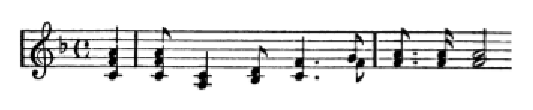
\includegraphics{texts/music.eps}
\end{center}

\noindent Between me and the other world there is ever an unasked
question: unasked by some through feelings of delicacy; by others
through the difficulty of rightly framing it. All, nevertheless,
flutter round it. They approach me in a half-hesitant sort of way, eye
me curiously or compassionately, and then, instead of saying directly,
How does it feel to be a problem? they say, I know an excellent
\page{2} colored man in my town; or, I fought at Mechanicsville; or,
Do not these Southern outrages make your blood boil? At these I smile,
or am interested, or reduce the boiling to a simmer, as the occasion
may require. To the real question, How does it feel to be a problem? I
answer seldom a word.

And yet, being a problem is a strange experience,---pe\-cu\-liar even
for one who has never been anything else, save perhaps in babyhood and
in Europe. It is in the early days of rollicking boyhood that the
revelation first bursts upon one, all in a day, as it were. I
remember well when the shadow swept across me. I was a little thing,
away up in the hills of New England, where the dark Housatonic winds
between Hoosac and Taghkanic to the sea. In a wee wooden schoolhouse,
something put it into the boys' and girls' heads to buy gorgeous
visiting-cards---ten cents a package---and exchange. The exchange was
merry, till one girl, a tall newcomer, refused my card,---re\-fused it
peremptorily, with a glance. Then it dawned upon me with a certain
suddenness that I was different from the others; or like, mayhap, in
heart and life and longing, but shut out from their world by a vast
veil. I had thereafter no desire to tear down that veil, to creep
through; I held all beyond it in common contempt, and lived above it
in a region of blue sky and great wandering shadows. That sky was
bluest when I could beat my mates at examination-time, or beat them at
a foot-race, or even beat their stringy heads. Alas, with the years
all this fine contempt began to fade; for the worlds I longed for, and
all their dazzling opportunities, were \page{3} theirs, not mine. But
they should not keep these prizes, I said; some, all, I would wrest
from them. Just how I would do it I could never decide: by reading
law, by healing the sick, by telling the wonderful tales that swam
in my head,---some way. With other black boys the strife was not so
fiercely sunny: their youth shrunk into tasteless sycophancy, or into
silent hatred of the pale world about them and mocking distrust of
everything white; or wasted itself in a bitter cry, Why did God make
me an outcast and a stranger in mine own house? The shades of the
prison-house closed round about us all: walls strait and stubborn to
the whitest, but relentlessly narrow, tall, and unscalable to sons
of night who must plod darkly on in resignation, or beat unavailing
palms against the stone, or steadily, half hopelessly, watch the
streak of blue above.

After the Egyptian and Indian, the Greek and Roman, the Teuton and
Mongolian, the Negro is a sort of seventh son, born with a veil, and
gifted with second-sight in this American world,---a world which
yields him no true self-consciousness, but only lets him see himself
through the revelation of the other world. It is a peculiar sensation,
this double-consciousness, this sense of always looking at one's self
through the eyes of others, of measuring one's soul by the tape of a
world that looks on in amused contempt and pity. One ever feels his
twoness,---an American, a Negro; two souls, two thoughts, two
unreconciled strivings; two warring ideals in one dark body, whose
dogged strength alone keeps it from being torn asunder.

\page{4}The history of the American Negro is the history of this
strife,---this longing to attain self-conscious manhood, to merge his
double self into a better and truer self. In this merging he wishes
neither of the older selves to be lost. He would not Africanize
America, for America has too much to teach the world and Africa. He
would not bleach his Negro soul in a flood of white Americanism, for
he knows that Negro blood has a message for the world. He simply
wishes to make it possible for a man to be both a Negro and an
American, without being cursed and spit upon by his fellows, without
having the doors of Opportunity closed roughly in his face.

This, then, is the end of his striving: to be a co-worker in the
kingdom of culture, to escape both death and isolation, to husband and
use his best powers and his latent genius. These powers of body and
mind have in the past been strangely wasted, dispersed, or forgotten.
The shadow of a mighty Negro past flits through the tale of Ethiopia
the Shadowy and of Egypt the Sphinx. Through history, the powers of
single black men flash here and there like falling stars, and die
sometimes before the world has rightly gauged their brightness. Here
in America, in the few days since Emancipation, the black man's
turning hither and thither in hesitant and doubtful striving has often
made his very strength to lose effectiveness, to seem like absence of
power, like weakness. And yet it is not weakness,---it is the
contradiction of double aims. The double-aimed struggle of the black
artisan---on the one hand to escape white contempt for a nation of
mere hewers of wood and drawers \page{5} of water, and on the other
hand to plough and nail and dig for a poverty-stricken horde---could
only result in making him a poor craftsman, for he had but half a
heart in either cause. By the poverty and ignorance of his people, the
Negro minister or doctor was tempted toward quackery and demagogy; and
by the criticism of the other world, toward ideals that made him
ashamed of his lowly tasks. The would-be black \textit{savant} was
confronted by the paradox that the knowledge his people needed was a
twice-told tale to his white neighbors, while the knowledge which
would teach the white world was Greek to his own flesh and blood. The
innate love of harmony and beauty that set the ruder souls of his
people a-dancing and a-singing raised but confusion and doubt in the
soul of the black artist; for the beauty revealed to him was the
soul-beauty of a race which his larger audience despised, and he could
not articulate the message of another people. This waste of double
aims, this seeking to satisfy two unreconciled ideals, has wrought sad
havoc with the courage and faith and deeds of ten thousand thousand
people,---has sent them often wooing false gods and invoking false
means of salvation, and at times has even seemed about to make them
ashamed of themselves.

Away back in the days of bondage they thought to see in one divine
event the end of all doubt and disappointment; few men ever worshipped
Freedom with half such unquestioning faith as did the American Negro
for two centuries. To him, so far as he thought and dreamed, slavery
was indeed the sum of all villainies, the cause of all sorrow, the
root of all \page{6} prejudice; Emancipation was the key to a promised
land of sweeter beauty than ever stretched before the eyes of wearied
Israelites. In song and exhortation swelled one refrain---Liberty; in
his tears and curses the God he implored had Freedom in his right
hand. At last it came,---suddenly, fearfully, like a dream. With one
wild carnival of blood and passion came the message in his own
plaintive cadences:---

\begin{verse}
``Shout, O children!\\
Shout, you're free!\\
For God has bought your liberty!''
\end{verse}

Years have passed away since then,---ten, twenty, forty; forty years
of national life, forty years of renewal and development, and yet the
swarthy spectre sits in its accustomed seat at the Nation's feast. In
vain do we cry to this our vastest social problem:---

\begin{verse}
``Take any shape but that, and my firm nerves\\
Shall never tremble!''
\end{verse}

The Nation has not yet found peace from its sins; the freedman has not
yet found in freedom his promised land. Whatever of good may have come
in these years of change, the shadow of a deep disappointment rests
upon the Negro people,---a disappointment all the more bitter because
the unattained ideal was unbounded save by the simple ignorance of a
lowly people.

The first decade was merely a prolongation of the vain search for
freedom, the boon that seemed ever barely to elude their grasp,---like
a tantalizing will-o'-the-wisp, maddening and misleading the
head-\page{7}less host. The holocaust of war, the terrors of the
Ku-Klux Klan, the lies of carpet-baggers, the disorganization of
industry, and the contradictory advice of friends and foes, left the
bewildered serf with no new watchword beyond the old cry for freedom.
As the time flew, however, he began to grasp a new idea. The ideal of
liberty demanded for its attainment powerful means, and these the
Fifteenth Amendment gave him. The ballot, which before he had looked
upon as a visible sign of freedom, he now regarded as the chief means
of gaining and perfecting the liberty with which war had partially
endowed him. And why not? Had not votes made war and emancipated
millions? Had not votes enfranchised the freedmen? Was anything
impossible to a power that had done all this? A million black men
started with renewed zeal to vote themselves into the kingdom. So the
decade flew away, the revolution of 1876 came, and left the half-free
serf weary, wondering, but still inspired. Slowly but steadily, in the
following years, a new vision began gradually to replace the dream of
political power,---a powerful movement, the rise of another ideal to
guide the unguided, another pillar of fire by night after a clouded
day. It was the ideal of ``book-learning''; the curiosity, born of
compulsory ignorance, to know and test the power of the cabalistic
letters of the white man, the longing to know. Here at last seemed to
have been discovered the mountain path to Canaan; longer than the
highway of Emancipation and law, steep and rugged, but straight,
leading to heights high enough to overlook life.

\page{8}Up the new path the advance guard toiled, slowly, heavily,
doggedly; only those who have watched and guided the faltering feet,
the misty minds, the dull understandings, of the dark pupils of these
schools know how faithfully, how piteously, this people strove to
learn. It was weary work. The cold statistician wrote down the inches
of progress here and there, noted also where here and there a foot had
slipped or some one had fallen. To the tired climbers, the horizon was
ever dark, the mists were often cold, the Canaan was always dim and
far away. If, however, the vistas disclosed as yet no goal, no
resting-place, little but flattery and criticism, the journey at least
gave leisure for reflection and self-examination; it changed the child
of Emancipation to the youth with dawning self-consciousness,
self-realization, self-respect. In those sombre forests of his
striving his own soul rose before him, and he saw
him\-self,---dark\-ly as through a veil; and yet he saw in himself
some faint revelation of his power, of his mission. He began to have a
dim feeling that, to attain his place in the world, he must be
himself, and not another. For the first time he sought to analyze the
burden he bore upon his back, that dead-weight of social degradation
partially masked behind a half-named Negro problem. He felt his
poverty; without a cent, without a home, without land, tools, or
savings, he had entered into competition with rich, landed, skilled
neighbors. To be a poor man is hard, but to be a poor race in a land
of dollars is the very bottom of hardships. He felt the weight of his
ignorance,---not simply of letters, but of life, of \page{9} business,
of the humanities; the accumulated sloth and shirking and awkwardness
of decades and centuries shackled his hands and feet. Nor was his
burden all poverty and ignorance. The red stain of bastardy, which two
centuries of systematic legal defilement of Negro women had stamped
upon his race, meant not only the loss of ancient African chastity,
but also the hereditary weight of a mass of corruption from white
adulterers, threatening almost the obliteration of the Negro home.

A people thus handicapped ought not to be asked to race with the
world, but rather allowed to give all its time and thought to its own
social problems. But alas! while sociologists gleefully count his
bastards and his prostitutes, the very soul of the toiling, sweating
black man is darkened by the shadow of a vast despair. Men call the
shadow prejudice, and learnedly explain it as the natural defence of
culture against barbarism, learning against ignorance, purity against
crime, the ``higher'' against the ``lower'' races. To which the Negro
cries Amen! and swears that to so much of this strange prejudice as is
founded on just homage to civilization, culture, righteousness, and
progress, he humbly bows and meekly does obeisance. But before that
nameless prejudice that leaps beyond all this he stands helpless,
dismayed, and well-nigh speechless; before that personal disrespect
and mockery, the ridicule and systematic humiliation, the distortion
of fact and wanton license of fancy, the cynical ignoring of the
better and the boisterous welcoming of the worse, the all-pervading
desire to inculcate disdain for everything \page{10} black, from
Toussaint to the devil,---be\-fore this there rises a sickening
despair that would disarm and discourage any nation save that black
host to whom ``discouragement'' is an unwritten word.

But the facing of so vast a prejudice could not but bring the
inevitable self-questioning, self-disparagement, and lowering of
ideals which ever accompany repression and breed in an atmosphere of
contempt and hate. Whisperings and portents came borne upon the four
winds: Lo! we are diseased and dying, cried the dark hosts; we cannot
write, our voting is vain; what need of education, since we must
always cook and serve? And the Nation echoed and enforced this
self-criticism, saying: Be content to be servants, and nothing more;
what need of higher culture for half-men? Away with the black man's
ballot, by force or fraud,---and behold the suicide of a race!
Nevertheless, out of the evil came something of good,---the more
careful adjustment of education to real life, the clearer perception
of the Negroes' social responsibilities, and the sobering realization
of the meaning of progress.

So dawned the time of \textit{Sturm und Drang}: storm and stress
to-day rocks our little boat on the mad waters of the world-sea; there
is within and without the sound of conflict, the burning of body and
rending of soul; inspiration strives with doubt, and faith with vain
questionings. The bright ideals of the past,---physical freedom,
political power, the training of brains and the training of
hands,---all these in turn have waxed and waned, until even the last
grows dim and overcast. Are they all wrong,---all false? No, not that,
but \page{11} each alone was over-simple and incomplete,---the dreams
of a credulous race-childhood, or the fond imaginings of the other
world which does not know and does not want to know our power. To be
really true, all these ideals must be melted and welded into one. The
training of the schools we need to-day more than ever,---the training
of deft hands, quick eyes and ears, and above all the broader, deeper,
higher culture of gifted minds and pure hearts. The power of the
ballot we need in sheer self-defence,---else what shall save us from a
second slavery? Freedom, too, the long-sought, we still seek,---the
freedom of life and limb, the freedom to work and think, the freedom
to love and aspire. Work, culture, liberty,---all these we need, not
singly but together, not successively but together, each growing and
aiding each, and all striving toward that vaster ideal that swims
before the Negro people, the ideal of human brotherhood, gained
through the unifying ideal of Race; the ideal of fostering and
developing the traits and talents of the Negro, not in opposition to
or contempt for other races, but rather in large conformity to the
greater ideals of the American Republic, in order that some day on
American soil two world-races may give each to each those
characteristics both so sadly lack. We the darker ones come even now
not altogether empty-handed: there are to-day no truer exponents of
the pure human spirit of the Declaration of Independence than the
American Negroes; there is no true American music but the wild sweet
melodies of the Negro slave; the American fairy tales and folk-lore
are Indian and African; and, all in all, we black men seem the sole
\page{12} oasis of simple faith and reverence in a dusty desert of
dollars and smartness. Will America be poorer if she replace her
brutal dyspeptic blundering with light-hearted but determined Negro
humility? or her coarse and cruel wit with loving jovial good-humor?
or her vulgar music with the soul of the Sorrow Songs?

Merely a concrete test of the underlying principles of the great
republic is the Negro Problem, and the spiritual striving of the
freedmen's sons is the travail of souls whose burden is almost beyond
the measure of their strength, but who bear it in the name of an
historic race, in the name of this the land of their fathers' fathers,
and in the name of human opportunity.

\vspace{1\baselineskip}

And now what I have briefly sketched in large outline let me on coming
pages tell again in many ways, with loving emphasis and deeper detail,
that men may listen to the striving in the souls of black folk.

% 1897/1903

\author{G. E. Moore}
\authdate{1873--1958}
\textdate{1903}
\addon{Principia Ethica, Chapter 1, excerpt}
\chapter{The Naturalistic Fallacy}
\source{moore1922}

\page{5}5. But our question `What is good?' may have still another
meaning. We may, in the third place, mean to ask, not what thing or
things are good, but how `good' is to be defined. This is an enquiry
which belongs only to Ethics, not to Casuistry; and this is the
enquiry which will occupy us first.

It is an enquiry to which most special attention should be directed;
since this question, how `good' is to be defined, is the most
fundamental in all Ethics. That which is meant by `good' is, in fact,
except its converse `bad,' the \textit{only} simple object of thought
which is peculiar to Ethics. Its definition is, therefore, the most
essential point in the definition of Ethics; and moreover a mistake
with regard to it entails a far larger number of erroneous ethical
judgments than any other. Unless this first question be fully
understood, and its true answer clearly recognised, the rest of Ethics
is as good as useless from the point of view of systematic knowledge.
True ethical judgments, of the two kinds last dealt with, may indeed
be made by those who do not know the answer to this question as well
as by those who do; and it goes without saying that the two classes of
people may lead equally good lives. But it is extremely unlikely that
the \textit{most general} ethical judgments will be equally valid, in
the absence of a true answer to this question: I shall presently try
to shew that the gravest errors have been largely due to \page{6}
beliefs in a false answer. And, in any case, it is impossible that,
till the answer to this question be known, any one should know
\textit{what is the evidence} for any ethical judgment whatsoever. But
the main object of Ethics, as a systematic science, is to give correct
\textit{reasons} for thinking that this or that is good; and, unless
this question be answered, such reasons cannot be given. Even,
therefore, apart from the fact that a false answer leads to false
conclusions, the present enquiry is a most necessary and important
part of the science of Ethics.

6. What, then, is good? How is good to be defined? Now, it may be
thought that this is a verbal question. A definition does indeed often
mean the expressing of one word's meaning in other words. But this is
not the sort of definition I am asking for. Such a definition can
never be of ultimate importance in any study except lexicography. If I
wanted that kind of definition I should have to consider in the first
place how people generally used the word `good'; but my business is
not with its proper usage, as established by custom. I should, indeed,
be foolish, if I tried to use it for something which it did not
usually denote: if, for instance, I were to announce that, whenever I
used the word `good,' I must be understood to be thinking of that
object which is usually denoted by the word `table.' I shall,
therefore, use the word in the sense in which I think it is ordinarily
used; but at the same time I am not anxious to discuss whether I am
right in thinking that it is so used. My business is solely with that
object or idea, which I hold, rightly or wrongly, that the word is
generally used to stand for. What I want to discover is the nature of
that object or idea, and about this I am extremely anxious to arrive
at an agreement.

But, if we understand the question in this sense, my answer to it may
seem a very disappointing one. If I am asked `What is good?' my answer
is that good is good, and that is the end of the matter. Or if I am
asked `How is good to be defined?' my answer is that it cannot be
defined, and that is all I have to say about it. But disappointing as
these answers may appear, they are of the very last importance. To
readers who are familiar with philosophic terminology, I can express
their im-\page{7}portance by saying that they amount to this: That
propositions about the good are all of them synthetic and never
analytic; and that is plainly no trivial matter. And the same thing
may be expressed more popularly, by saying that, if I am right, then
nobody can foist upon us such an axiom as that `Pleasure is the only
good' or that `The good is the desired' on the pretence that this is
`the very meaning of the word.'

7. Let us, then, consider this position. My point is that `good' is a
simple notion, just as `yellow' is a simple notion; that, just as you
cannot, by any manner of means, explain to any one who does not
already know it, what yellow is, so you cannot explain what good is.
Definitions of the kind that I was asking for, definitions which
describe the real nature of the object or notion denoted by a word,
and which do not merely tell us what the word is used to mean, are
only possible when the object or notion in question is something
complex. You can give a definition of a horse, because a horse has
many different properties and qualities, all of which you can
enumerate. But when you have enumerated them all, when you have
reduced a horse to his simplest terms, then you can no longer define
those terms. They are simply something which you think of or perceive,
and to any one who cannot think of or perceive them, you can never, by
any definition, make their nature known. It may perhaps be objected to
this that we are able to describe to others, objects which they have
never seen or thought of. We can, for instance, make a man understand
what a chimaera is, although he has never heard of one or seen one.
You can tell him that it is an animal with a lioness's head and body,
with a goat's head growing from the middle of its back, and with a
snake in place of a tail. But here the object which you are describing
is a complex object; it is entirely composed of parts, with which we
are all perfectly familiar---a snake, a goat, a lioness; and we know,
too, the manner in which those parts are to be put together, because
we know what is meant by the middle of a lioness's back, and where her
tail is wont to grow. And so it is with all objects, not previously
known, which we are able to define: they are all complex; all composed
of parts, which may themselves, in the \page{8} first instance, be
capable of similar definition, but which must in the end be reducible
to simplest parts, which can no longer be defined. But yellow and
good, we say, are not complex: they are notions of that simple kind,
out of which definitions are composed and with which the power of
further defining ceases.

8. When we say, as Webster says, `The definition of horse is ``A
hoofed quadruped of the genus Equus,''' we may, in fact, mean three
different things. (1) We may mean merely: `When I say ``horse,'' you
are to understand that I am talking about a hoofed quadruped of the
genus Equus.' This might be called the arbitrary verbal definition:
and I do not mean that good is indefinable in that sense. (2) We may
mean, as Webster ought to mean: `When most English people say
``horse,'' they mean a hoofed quadruped of the genus Equus.' This may
be called the verbal definition proper, and I do not say that good is
indefinable in this sense either; for it is certainly possible to
discover how people use a word: otherwise, we could never have known
that `good' may be translated by `gut' in German and by `bon' in
French. But (3) we may, when we define horse, mean something much more
important. We may mean that a certain object, which we all of us know,
is composed in a certain manner: that it has four legs, a head, a
heart, a liver, etc., etc., all of them arranged in definite relations
to one another. It is in this sense that I deny good to be definable.
I say that it is not composed of any parts, which we can substitute
for it in our minds when we are thinking of it. We might think just as
clearly and correctly about a horse, if we thought of all its parts
and their arrangement instead of thinking of the whole: we could, I
say, think how a horse differed from a donkey just as well, just as
truly, in this way, as now we do, only not so easily; but there is
nothing whatsoever which we could so substitute for good; and that is
what I mean, when I say that good is indefinable.

9. But I am afraid I have still not removed the chief difficulty which
may prevent acceptance of the proposition that good is indefinable. I
do not mean to say that \textit{the} good, that which is good, is thus
indefinable; if I did think so, I should not \page{9} be writing on
Ethics, for my main object is to help towards discovering that
definition. It is just because I think there will be less risk of
error in our search for a definition of `the good,' that I am now
insisting that \textit{good} is indefinable. I must try to explain the
difference between these two. I suppose it may be granted that `good'
is an adjective. Well `the good,' `that which is good,' must therefore
be the substantive to which the adjective `good' will apply: it must
be the whole of that to which the adjective will apply, and the
adjective must \textit{always} truly apply to it. But if it is that to
which the adjective will apply, it must be something different from
that adjective itself; and the whole of that something different,
whatever it is, will be our definition of \textit{the} good. Now it
may be that this something will have other adjectives, beside `good,'
that will apply to it. It may be full of pleasure, for example; it may
be intelligent: and if these two adjectives are really part of its
definition, then it will certainly be true, that pleasure and
intelligence are good. And many people appear to think that, if we say
`Pleasure and intelligence are good,' or if we say `Only pleasure and
intelligence are good,' we are defining `good.' Well, I cannot deny
that propositions of this nature may sometimes be called definitions;
I do not know well enough how the word is generally used to decide
upon this point. I only wish it to be understood that that is not what
I mean when I say there is no possible definition of good, and that I
shall not mean this if I use the word again. I do most fully believe
that some true proposition of the form `Intelligence is good and
intelligence alone is good' can be found; if none could be found, our
definition of \textit{the} good would be impossible. As it is, I
believe \textit{the} good to be definable; and yet I still say that
good itself is indefinable.

10. `Good,' then, if we mean by it that quality which we assert to
belong to a thing, when we say that the thing is good, is incapable of
any definition, in the most important sense of that word. The most
important sense of `definition' is that in which a definition states
what are the parts which invariably compose a certain whole; and in
this sense `good' has no definition because it is simple and has no
parts. It is one of \page{10} those innumerable objects of thought
which are themselves incapable of definition, because they are the
ultimate terms by reference to which whatever \textit{is} capable of
definition must be defined. That there must be an indefinite number of
such terms is obvious, on reflection; since we cannot define anything
except by an analysis, which, when carried as far as it will go,
refers us to something, which is simply different from anything else,
and which by that ultimate difference explains the peculiarity of the
whole which we are defining: for every whole contains some parts which
are common to other wholes also. There is, therefore, no intrinsic
difficulty in the contention that `good' denotes a simple and
indefinable quality. There are many other instances of such qualities.

Consider yellow, for example. We may try to define it, by describing
its physical equivalent; we may state what kind of light-vibrations
must stimulate the normal eye, in order that we may perceive it. But a
moment's reflection is sufficient to shew that those light-vibrations
are not themselves what we mean by yellow. \textit{They} are not what
we perceive. Indeed we should never have been able to discover their
existence, unless we had first been struck by the patent difference of
quality between the different colours. The most we can be entitled to
say of those vibrations is that they are what corresponds in space to
the yellow which we actually perceive.

Yet a mistake of this simple kind has commonly been made about `good.'
It may be true that all things which are good are \textit{also}
something else, just as it is true that all things which are yellow
produce a certain kind of vibration in the light. And it is a fact,
that Ethics aims at discovering what are those other properties
belonging to all things which are good. But far too many philosophers
have thought that when they named those other properties they were
actually defining good; that these properties, in fact, were simply
not `other,' but absolutely and entirely the same with goodness. This
view I propose to call the `naturalistic fallacy' and of it I shall
now endeavour to dispose.

11. Let us consider what it is such philosophers say. And first it is
to be noticed that they do not agree among themselves. \page{11} They
not only say that they are right as to what good is, but they
endeavour to prove that other people who say that it is something
else, are wrong. One, for instance, will affirm that good is pleasure,
another, perhaps, that good is that which is desired; and each of
these will argue eagerly to prove that the other is wrong. But how is
that possible? One of them says that good is nothing but the object of
desire, and at the same time tries to prove that it is not pleasure.
But from his first assertion, that good just means the object of
desire, one of two things must follow as regards his proof:

(1) He may be trying to prove that the object of desire is not
pleasure. But, if this be all, where is his Ethics? The position he is
maintaining is merely a psychological one. Desire is something which
occurs in our minds, and pleasure is something else which so occurs;
and our would-be ethical philosopher is merely holding that the latter
is not the object of the former. But what has that to do with the
question in dispute? His opponent held the ethical proposition that
pleasure was the good, and although he should prove a million times
over the psychological proposition that pleasure is not the object of
desire, he is no nearer proving his opponent to be wrong. The position
is like this. One man says a triangle is a circle: another replies `A
triangle is a straight line, and I will prove to you that I am right:
\textit{for}' (this is the only argument) `a straight line is not a
circle.' `That is quite true,' the other may reply; `but nevertheless
a triangle is a circle, and you have said nothing whatever to prove
the contrary. What is proved is that one of us is wrong, for we agree
that a triangle cannot be both a straight line and a circle: but which
is wrong, there can be no earthly means of proving, since you define
triangle as straight line and I define it as circle.'---Well, that is
one alternative which any naturalistic Ethics has to face; if good is
\textit{defined} as something else, it is then impossible either to
prove that any other definition is wrong or even to deny such
definition.

(2) The other alternative will scarcely be more welcome. It is that
the discussion is after all a verbal one. When A says `Good means
pleasant' and B says `Good means desired,' they may merely wish to
assert that most people have used the word \page{12} for what is
pleasant and for what is desired respectively. And this is quite an
interesting subject for discussion: only it is not a whit more an
ethical discussion than the last was. Nor do I think that any exponent
of naturalistic Ethics would be willing to allow that this was all he
meant. They are all so anxious to persuade us that what they call the
good is what we really ought to do. `Do, pray, act so, because the
word ``good'' is generally used to denote actions of this nature':
such, on this view, would be the substance of their teaching. And in
so far as they tell us how we ought to act, their teaching is truly
ethical, as they mean it to be. But how perfectly absurd is the reason
they would give for it! `You are to do this, because most people use a
certain word to denote conduct such as this.' `You are to say the
thing which is not, because most people call it lying.' That is an
argument just as good!---My dear sirs, what we want to know from you
as ethical teachers, is not how people use a word; it is not even,
what kind of actions they approve, which the use of this word `good'
may certainly imply: what we want to know is simply what \textit{is}
good. We may indeed agree that what most people do think good, is
actually so; we shall at all events be glad to know their opinions:
but when we say their opinions about what \textit{is} good, we do mean
what we say; we do not care whether they call that thing which they
mean `horse' or `table' or `chair,' `gut' or `bon' or `\grk{ἀγαθός}';
we want to know what it is that they so call. When they say `Pleasure
is good,' we cannot believe that they merely mean `Pleasure is
pleasure' and nothing more than that.

12. Suppose a man says `I am pleased'; and suppose that is not a lie
or a mistake but the truth. Well, if it is true, what does that mean?
It means that his mind, a certain definite mind, distinguished by
certain definite marks from all others, has at this moment a certain
definite feeling called pleasure. `Pleased' \textit{means} nothing but
having pleasure, and though we may be more pleased or less pleased,
and even, we may admit for the present, have one or another kind of
pleasure; yet in so far as it is pleasure we have, whether there be
more or less of it, and whether it be of one kind or another, what we
have is \page{13} one definite thing, absolutely indefinable, some one
thing that is the same in all the various degrees and in all the
various kinds of it that there may be. We may be able to say how it is
related to other things: that, for example, it is in the mind, that it
causes desire, that we are conscious of it, etc., etc. We can, I say,
describe its relations to other things, but define it we can
\textit{not}. And if anybody tried to define pleasure for us as being
any other natural object; if anybody were to say, for instance, that
pleasure \textit{means} the sensation of red, and were to proceed to
deduce from that that pleasure is a colour, we should be entitled to
laugh at him and to distrust his future statements about pleasure.
Well, that would be the same fallacy which I have called the
naturalistic fallacy. That `pleased' does not mean `having the
sensation of red,' or anything else whatever, does not prevent us from
understanding what it does mean. It is enough for us to know that
`pleased' does mean `having the sensation of pleasure,' and though
pleasure is absolutely indefinable, though pleasure is pleasure and
nothing else whatever, yet we feel no difficulty in saying that we are
pleased. The reason is, of course, that when I say `I am pleased,' I
do \textit{not} mean that `I' am the same thing as `having pleasure.'
And similarly no difficulty need be found in my saying that `pleasure
is good' and yet not meaning that `pleasure' is the same thing as
`good,' that pleasure \textit{means} good, and that good
\textit{means} pleasure. If I were to imagine that when I said `I am
pleased,' I meant that I was exactly the same thing as `pleased,' I
should not indeed call that a naturalistic fallacy, although it would
be the same fallacy as I have called naturalistic with reference to
Ethics. The reason of this is obvious enough. When a man confuses
two natural objects with one another, defining the one by the other,
if for instance, he confuses himself, who is one natural object, with
`pleased' or with `pleasure' which are others, then there is no reason
to call the fallacy naturalistic. But if he confuses `good,' which
is not in the same sense a natural object, with any natural object
whatever, then there is a reason for calling that a naturalistic
fallacy; its being made with regard to `good' marks it as something
quite specific, and this specific mistake deserves a name because it
is so common. \page{14} As for the reasons why good is not to be
considered a natural object, they may be reserved for discussion in
another place. But, for the present, it is sufficient to notice
this: Even if it were a natural object, that would not alter the
nature of the fallacy nor diminish its importance one whit. All that I
have said about it would remain quite equally true: only the name
which I have called it would not be so appropriate as I think it is.
And I do not care about the name: what I do care about is the fallacy.
It does not matter what we call it, provided we recognise it when we
meet with it. It is to be met with in almost every book on Ethics; and
yet it is not recognised: and that is why it is necessary to multiply
illustrations of it, and convenient to give it a name. It is a very
simple fallacy indeed. When we say that an orange is yellow, we do not
think our statement binds us to hold that `orange' means nothing else
than `yellow,' or that nothing can be yellow but an orange. Supposing
the orange is also sweet! Does that bind us to say that `sweet' is
exactly the same thing as `yellow,' that `sweet' must be defined as
`yellow'? And supposing it be recognised that `yellow' just means
`yellow' and nothing else whatever, does that make it any more
difficult to hold that oranges are yellow? Most certainly it does not:
on the contrary, it would be absolutely meaningless to say that
oranges were yellow, unless yellow did in the end mean just `yellow'
and nothing else whatever---unless it was absolutely indefinable. We
should not get any very clear notion about things, which are
yellow---we should not get very far with our science, if we were bound
to hold that everything which was yellow, \textit{meant} exactly the
same thing as yellow. We should find we had to hold that an orange was
exactly the same thing as a stool, a piece of paper, a lemon, anything
you like. We could prove any number of absurdities; but should we be
the nearer to the truth? Why, then, should it be different with
`good'? Why, if good is good and indefinable, should I be held to deny
that pleasure is good? Is there any difficulty in holding both to be
true at once? On the contrary, there is no meaning in saying that
pleasure is good, unless good is something different from pleasure. It
is absolutely useless, so far as Ethics is concerned, to prove, as Mr
Spencer \page{15} tries to do, that increase of pleasure coincides
with increase of life, unless good \textit{means} something different
from either life or pleasure. He might just as well try to prove that
an orange is yellow by shewing that it always is wrapped up in
paper.

13. In fact, if it is not the case that `good' denotes something
simple and indefinable, only two alternatives are possible: either it
is a complex, a given whole, about the correct analysis of which there
may be disagreement; or else it means nothing at all, and there is no
such subject as Ethics. In general, however, ethical philosophers have
attempted to define good, without recognising what such an attempt
must mean. They actually use arguments which involve one or both of
the absurdities considered in \S11. We are, therefore, justified in
concluding that the attempt to define good is chiefly due to want of
clearness as to the possible nature of definition. There are, in fact,
only two serious alternatives to be considered, in order to establish
the conclusion that `good' does denote a simple and indefinable
notion. It might possibly denote a complex, as `horse' does; or it
might have no meaning at all. Neither of these possibilities has,
however, been clearly conceived and seriously maintained, as such, by
those who presume to define good; and both may be dismissed by a
simple appeal to facts.

(1) The hypothesis that disagreement about the meaning of good is
disagreement with regard to the correct analysis of a given whole, may
be most plainly seen to be incorrect by consideration of the fact
that, whatever definition be offered, it may be always asked, with
significance, of the complex so defined, whether it is itself good. To
take, for instance, one of the more plausible, because one of the more
complicated, of such proposed definitions, it may easily be thought,
at first sight, that to be good may mean to be that which we desire to
desire. Thus if we apply this definition to a particular instance and
say `When we think that A is good, we are thinking that A is one of
the things which we desire to desire,' our proposition may seem quite
plausible. But, if we carry the investigation further, and ask
ourselves `Is it good to desire to desire A?' it is apparent, on a
little reflection, that this question is itself as intelligible, as
the original question `Is A good?'---that we are, \page{16} in fact,
now asking for exactly the same information about the desire to desire
A, for which we formerly asked with regard to A itself. But it is also
apparent that the meaning of this second question cannot be correctly
analysed into `Is the desire to desire A one of the things which we
desire to desire?': we have not before our minds anything so
complicated as the question `Do we desire to desire to desire to
desire A?' Moreover any one can easily convince himself by inspection
that the predicate of this proposition---`good'---is positively
different from the notion of `desiring to desire' which enters into
its subject: `That we should desire to desire A is good' is
\textit{not} merely equivalent to `That A should be good is good.' It
may indeed be true that what we desire to desire is always also good;
perhaps, even the converse may be true: but it is very doubtful
whether this is the case, and the mere fact that we understand very
well what is meant by doubting it, shews clearly that we have two
different notions before our minds.

(2) And the same consideration is sufficient to dismiss the hypothesis
that `good' has no meaning whatsoever. It is very natural to make the
mistake of supposing that what is universally true is of such a nature
that its negation would be self-contradictory: the importance which
has been assigned to analytic propositions in the history of
philosophy shews how easy such a mistake is. And thus it is very easy
to conclude that what seems to be a universal ethical principle is in
fact an identical proposition; that, if, for example, whatever is
called `good' seems to be pleasant, the proposition `Pleasure is the
good' does not assert a connection between two different notions, but
involves only one, that of pleasure, which is easily recognised as a
distinct entity. But whoever will attentively consider with himself
what is actually before his mind when he asks the question `Is
pleasure (or whatever it may be) after all good?' can easily satisfy
himself that he is not merely wondering whether pleasure is pleasant.
And if he will try this experiment with each suggested definition in
succession, he may become expert enough to recognise that in every
case he has before his mind a unique object, with regard to the
connection of which with any other object, a distinct question may be
asked. Every \page{17} one does in fact understand the question `Is
this good?' When he thinks of it, his state of mind is different from
what it would be, were he asked `Is this pleasant, or desired, or
approved?' It has a distinct meaning for him, even though he may not
recognise in what respect it is distinct. Whenever he thinks of
`intrinsic value,' or `intrinsic worth,' or says that a thing `ought
to exist,' he has before his mind the unique object---the unique
property of things---which I mean by `good.' Everybody is constantly
aware of this notion, although he may never become aware at all that
it is different from other notions of which he is also aware. But, for
correct ethical reasoning, it is extremely important that he should
become aware of this fact; and, as soon as the nature of the problem
is clearly understood, there should be little difficulty in advancing
so far in analysis.

14. `Good,' then, is indefinable; and yet, so far as I know, there is
only one ethical writer, Prof. Henry Sidgwick, who has clearly
recognised and stated this fact. We shall see, indeed, how far many of
the most reputed ethical systems fall short of drawing the conclusions
which follow from such a recognition. At present I will only quote one
instance, which will serve to illustrate the meaning and importance of
this principle that `good' is indefinable, or, as Prof. Sidgwick says,
an `unanalysable notion.' It is an instance to which Prof. Sidgwick
himself refers in a note on the passage, in which he argues that
`ought' is unanalysable\footnote{\textit{Methods of Ethics}, Bk. I,
Chap. iii, \S1 (6th edition).}.

`Bentham,' says Sidgwick, `explains that his fundamental principle
``states the greatest happiness of all those whose interest is in
question as being the right and proper end of human action'''; and yet
`his language in other passages of the same chapter would seem to
imply' that he \textit{means} by the word ``right'' ``conducive to the
general happiness.'' Prof. Sidgwick sees that, if you take these two
statements together, you get the absurd result that `greatest
happiness is the end of human action, which is conducive to the
general happiness'; and so absurd does it seem to him to call this
result, as Bentham calls it, `the fundamental principle of a moral
system,' that he suggests that Bentham cannot have meant it. Yet Prof.
Sidgwick \page{18} himself states elsewhere\footnote{\textit{Methods
of Ethics}, Bk. I, Chap. iv, \S1.} that Psychological Hedonism is `not
seldom confounded with Egoistic Hedonism'; and that confusion, as we
shall see, rests chiefly on that same fallacy, the naturalistic
fallacy, which is implied in Bentham's statements. Prof. Sidgwick
admits therefore that this fallacy is sometimes committed, absurd as
it is; and I am inclined to think that Bentham may really have been
one of those who committed it. Mill, as we shall see, certainly did
commit it. In any case, whether Bentham committed it or not, his
doctrine, as above quoted, will serve as a very good illustration of
this fallacy, and of the importance of the contrary proposition that
good is indefinable.

Let us consider this doctrine. Bentham seems to imply, so Prof.
Sidgwick says, that the word `right' \textit{means} `conducive to
general happiness.' Now this, by itself, need not necessarily involve
the naturalistic fallacy. For the word `right' is very commonly
appropriated to actions which lead to the attainment of what is good;
which are regarded as \textit{means} to the ideal and not as
ends-in-themselves. This use of `right,' as denoting what is good as a
means, whether or not it be also good as an end, is indeed the use to
which I shall confine the word. Had Bentham been using `right' in this
sense, it might be perfectly consistent for him to \textit{define}
right as `conducive to the general happiness,' \textit{provided only}
(and notice this proviso) he had already proved, or laid down as an
axiom, that general happiness was \textit{the} good, or (what is
equivalent to this) that general happiness alone was good. For in that
case he would have already defined \textit{the} good as general
happiness (a position perfectly consistent, as we have seen, with the
contention that `good' is indefinable), and, since right was to be
defined as `conducive to \textit{the} good,' it would actually
\textit{mean} `conducive to general happiness.' But this method of
escape from the charge of having committed the naturalistic fallacy
has been closed by Bentham himself. For his fundamental principle is,
we see, that the greatest happiness of all concerned is the
\textit{right} and proper \textit{end} of human action. He applies the
word `right,' therefore, to the end, as such, not only to the means
which are \page{19} conducive to it; and, that being so, right can no
longer be defined as `conducive to the general happiness,' without
involving the fallacy in question. For now it is obvious that the
definition of right as conducive to general happiness can be used by
him in support of the fundamental principle that general happiness is
the right end; instead of being itself derived from that principle. If
right, by definition, means conducive to general happiness, then it is
obvious that general happiness is the right end. It is not necessary
now first to prove or assert that general happiness is the right end,
before right is defined as conducive to general happiness---a
perfectly valid procedure; but on the contrary the definition of right
as conducive to general happiness proves general happiness to be the
right end---a perfectly invalid procedure, since in this case the
statement that `general happiness is the right end of human action' is
not an ethical principle at all, but either, as we have seen, a
proposition about the meaning of words, or else a proposition about
the \textit{nature} of general happiness, not about its rightness or
goodness.

Now, I do not wish the importance I assign to this fallacy to be
misunderstood. The discovery of it does not at all refute Bentham's
contention that greatest happiness is the proper end of human action,
if that be understood as an ethical proposition, as he undoubtedly
intended it. That principle may be true all the same; we shall
consider whether it is so in succeeding chapters. Bentham might have
maintained it, as Professor Sidgwick does, even if the fallacy had
been pointed out to him. What I am maintaining is that the
\textit{reasons} which he actually gives for his ethical proposition
are fallacious ones so far as they consist in a definition of right.
What I suggest is that he did not perceive them to be fallacious;
that, if he had done so, he would have been led to seek for other
reasons in support of his Utilitarianism; and that, had he sought for
other reasons, he \textit{might} have found none which he thought to
be sufficient. In that case he would have changed his whole system---a
most important consequence. It is undoubtedly also possible that he
would have thought other reasons to be sufficient, and in that case
his ethical system, \page{20} in its main results, would still have
stood. But, even in this latter case, his use of the fallacy would be
a serious objection to him as an ethical philosopher. For it is the
business of Ethics, I must insist, not only to obtain true results,
but also to find valid reasons for them. The direct object of Ethics
is knowledge and not practice; and any one who uses the naturalistic
fallacy has certainly not fulfilled this first object, however correct
his practical principles may be.

My objections to Naturalism are then, in the first place, that it
offers no reason at all, far less any valid reason, for any ethical
principle whatever; and in this it already fails to satisfy the
requirements of Ethics, as a scientific study. But in the second place
I contend that, though it gives a reason for no ethical principle, it
is a \textit{cause} of the acceptance of false principles---it deludes
the mind into accepting ethical principles, which are false; and in
this it is contrary to every aim of Ethics. It is easy to see that if
we start with a definition of right conduct as conduct conducive to
general happiness; then, knowing that right conduct is universally
conduct conducive to the good, we very easily arrive at the result
that the good is general happiness. If, on the other hand, we once
recognise that we must start our Ethics without a definition, we shall
be much more apt to look about us, before we adopt any ethical
principle whatever; and the more we look about us, the less likely are
we to adopt a false one. It may be replied to this: Yes, but we shall
look about us just as much, before we settle on our definition, and
are therefore just as likely to be right. But I will try to shew that
this is not the case. If we start with the conviction that a
definition of good can be found, we start with the conviction that
good \textit{can mean} nothing else than some one property of things;
and our only business will then be to discover what that property is.
But if we recognise that, so far as the meaning of good goes, anything
whatever may be good, we start with a much more open mind. Moreover,
apart from the fact that, when we think we have a definition, we
cannot logically defend our ethical principles in any way whatever, we
shall also be much less apt to defend them well, even if illogically.
For we shall start with the conviction that good \page{21} must mean
so and so, and shall therefore be inclined either to misunderstand our
opponent's arguments or to cut them short with the reply, `This is not
an open question: the very meaning of the word decides it; no one can
think otherwise except through confusion.'

% 1903

%\author{Mark Twain [Samuel Clemens]}
\author{Mark Twain}
\authdate{1835--1910}
\textdate{1904/5}
\chapter[Mark Twain -- The War Prayer]{The War Prayer}

\nfootnote{\fullcite{twain1923.34}}

\page{394}It was a time of great and exalting excitement. The country
was up in arms, the war was on, in every breast burned the holy fire
of patriotism; the drums were beating, the bands playing, the toy
pistols popping, the bunched firecrackers hissing and spluttering; on
every hand and far down the receding and fading spread of roofs and
balconies a fluttering wilderness of flags flashed in the sun; daily
the young volunteers marched down the wide avenue gay and fine in
their new uniforms, the proud fathers and mothers and sisters and
sweethearts cheering them with voices choked with happy emotion as
they swung by; nightly the packed mass meetings listened, panting, to
patriot oratory which stirred the deepest deeps of their hearts, and
which they interrupted at briefest intervals with cyclones of
applause, the tears running down their cheeks the while; in the
churches the pastors preached devotion to flag and country, and
invoked the God of Battles beseeching His aid in our good cause in
outpourings of fervid eloquence which moved every listener. It was
indeed a glad and gracious time, and the half dozen rash spirits that
ventured to disapprove of the war and cast a doubt upon its
righteousness straightway got such a stern and angry \page{395}
warning that for their personal safety's sake they quickly shrank out
of sight and offended no more in that way.

% NOTE: text has 'them home from the war'

Sunday morning came---next day the battalions would leave for the
front; the church was filled; the volunteers were there, their young
faces alight with martial dreams---vi\-sions of the stern advance, the
gathering momentum, the rushing charge, the flashing sabers, the
flight of the foe, the tumult, the enveloping smoke, the fierce
pursuit, the surrender!---then home from the war, bronzed heroes,
welcomed, adored, submerged in golden seas of glory! With the
volunteers sat their dear ones, proud, happy, and envied by the
neighbors and friends who had no sons and brothers to send forth to
the field of honor, there to win for the flag, or, failing, die the
noblest of noble deaths. The service proceeded; a war chapter from the
Old Testament was read; the first prayer was said; it was followed by
an organ burst that shook the building, and with one impulse the house
rose, with glowing eyes and beating hearts, and poured out that
tremendous invocation---

\begin{verse}
``God the all-terrible! Thou who ordainest,\\
Thunder thy clarion and lightning thy sword!''
\end{verse}

\noindent Then came the ``long'' prayer. None could remember the like
of it for passionate pleading and moving and beautiful language. The
burden of its supplication was, that an ever-merciful and benignant
Father of us all would watch over our noble young soldiers, and aid,
comfort, and encourage them in their patriotic work; bless them,
shield them in the day of battle \page{396} and the hour of peril,
bear them in His mighty hand, make them strong and confident,
invincible in the bloody onset; help them to crush the foe, grant to
them and to their flag and country imperishable honor and glory---

An aged stranger entered and moved with slow and noiseless step up the
main aisle, his eyes fixed upon the minister, his long body clothed in
a robe that reached to his feet, his head bare, his white hair
descending in a frothy cataract to his shoulders, his seamy face
unnaturally pale, pale even to ghastliness. With all eyes following
him and wondering, he made his silent way; without pausing, he
ascended to the preacher's side and stood there, waiting. With shut
lids the preacher, unconscious of his presence, continued with his
moving prayer, and at last finished it with the words, uttered in
fervent appeal, ``Bless our arms, grant us the victory, O Lord our
God, Father and Protector of our land and flag!''

The stranger touched his arm, motioned him to step a\-side---which the
startled minister did---and took his place. During some moments he
surveyed the spellbound audience with solemn eyes, in which burned an
uncanny light; then in a deep voice he said:

``I come from the Throne---bear\-ing a message from Almighty God!''
The words smote the house with a shock; if the stranger perceived it
he gave no attention. ``He has heard the prayer of His servant your
shepherd, and will grant it if such shall be your desire after I, His
messenger, shall have explained to you its im\-port---that is to say,
its full import. \page{397} For it is like unto many of the prayers of
men, in that it asks for more than he who utters it is aware
of---except he pause and think.

``God's servant and yours has prayed his prayer. Has he paused and
taken thought? Is it one prayer? No, it is two---one uttered, the
other not. Both have reached the ear of Him Who heareth all
supplications, the spoken and the unspoken. Ponder this---keep it in
mind. If you would beseech a blessing upon yourself, beware! lest
without intent you invoke a curse upon a neighbor at the same time. If
you pray for the blessing of rain upon your crop which needs it, by
that act you are possibly praying for a curse upon some neighbor's
crop which may not need rain and can be injured by it.

``You have heard your servant's prayer---the uttered part of it. I am
commissioned of God to put into words the other part of it---that part
which the pas\-tor---and also you in your hearts---fervently prayed
silently. And ignorantly and unthinkingly? God grant that it was so!
You heard these words: `Grant us the victory, O Lord our God!' That is
sufficient. The \textit{whole} of the uttered prayer is compact into
those pregnant words. Elaborations were not necessary. When you have
prayed for victory you have prayed for many unmentioned results which
follow vic\-to\-ry---\textit{must} follow it, cannot help but follow
it. Upon the listening spirit of God the Father fell also the unspoken
part of the prayer. He commandeth me to put it into words. Listen!

``O Lord our Father, our young patriots, idols of \page{398} our
hearts, go forth to bat\-tle---be Thou near them! With them---in
spir\-it---we also go forth from the sweet peace of our beloved
firesides to smite the foe. O Lord our God, help us to tear their
soldiers to bloody shreds with our shells; help us to cover their
smiling fields with the pale forms of their patriot dead; help us to
drown the thunder of the guns with the shrieks of their wounded,
writhing in pain; help us to lay waste their humble homes with a
hurricane of fire; help us to wring the hearts of their unoffending
widows with unavailing grief; help us to turn them out roofless with
little children to wander unfriended the wastes of their desolated
land in rags and hunger and thirst, sports of the sun flames of summer
and the icy winds of winter, broken in spirit, worn with travail,
imploring Thee for the refuge of the grave and denied it---for our
sakes who adore Thee, Lord, blast their hopes, blight their lives,
protract their bitter pilgrimage, make heavy their steps, water their
way with their tears, stain the white snow with the blood of their
wounded feet! We ask it, in the spirit of love, of Him Who is the
Source of Love, and Who is the ever-faithful refuge and friend of all
that are sore beset and seek His aid with humble and contrite hearts.
Amen.''

(\textit{After a pause}.) ``Ye have prayed it; if ye still desire it,
speak! The messenger of the Most High waits!''

It was believed afterward that the man was a lunatic, because there
was no sense in what he said.

% 1904/5

\author{Emma Goldman}
\authdate{1869--1940}
\textdate{1906}
\chapter{The Tragedy of Woman's Emancipation}
\source{goldman1917.11}

% First published in Mother Earth in March 1906.

\page{219}\noindent I begin with an admission: Regardless of all
political and economic theories, treating of the fundamental
differences between various groups within the human race, regardless
of class and race distinctions, regardless of all artificial boundary
lines between woman's rights and man's rights, I hold that there is a
point where these differentiations may meet and grow into one perfect
whole.

With this I do not mean to propose a peace treaty. The general social
antagonism which has taken hold of our entire public life today,
brought about through the force of opposing and contradictory
interests, will crumble to pieces when the reorganization of our
social life, based upon the principles of economic justice, shall have
become a reality.

Peace or harmony between the sexes and individuals does not
necessarily depend on a superficial equalization of human beings; nor
does it call for the elimination of individual traits and
peculiarities. The problem that confronts us today, and which the
nearest future is to solve, is how to be one's self and yet \page{220}
in oneness with others, to feel deeply with all human beings and still
retain one's own characteristic qualities. This seems to me to be the
basis upon which the mass and the individual, the true democrat and
the true individuality, man and woman, can meet without antagonism and
opposition. The motto should not be: Forgive one another; rather,
Understand one another. The oft-quoted sentence of Madame de
Sta\"{e}l:  ``To understand everything means to forgive everything,''
has never particularly appealed to me; it has the odor of the
confessional; to forgive one's fellow-being conveys the idea of
pharisaical superiority. To understand one's fellow-being suffices.
The admission partly represents the fundamental aspect of my views on
the emancipation of woman and its effect upon the entire sex.

Emancipation should make it possible for woman to be human in the
truest sense. Everything within her that craves assertion and activity
should reach its fullest expression; all artificial barriers should be
broken, and the road towards greater freedom cleared of every trace of
centuries of submission and slavery.

This was the original aim of the movement for woman's emancipation.
But the results so far achieved have isolated woman and have robbed
her of the fountain springs of that happiness which is so essential to
her. Merely external emancipation has made of the modern woman an
artificial being, who reminds one of the products of French
arboriculture with its arabesque trees and shrubs, pyramids, wheels,
and wreaths; anything, except the forms which would be reached by the
expression of her own inner quali-\page{221}ties. Such artificially
grown plants of the female sex are to be found in large numbers,
especially in the so-called intellectual sphere of our life.

Liberty and equality for woman! What hopes and aspirations these words
awakened when they were first uttered by some of the noblest and
bravest souls of those days. The sun in all his light and glory was to
rise upon a new world; in this world woman was to be free to direct
her own destiny---an aim certainly worthy of the great enthusiasm,
courage, perseverance, and ceaseless effort of the tremendous host of
pioneer men and women, who staked everything against a world of
prejudice and ignorance.

% Without '\linebreak', an overfull hbox warning:

My hopes also move towards that goal, but I hold that the emancipation
of \linebreak[4] woman, as interpreted and practically applied today,
has failed to reach that great end. Now, woman is confronted with the
necessity of emancipating herself from emancipation, if she really
desires to be free. This may sound paradoxical, but is, nevertheless,
only too true.

What has she achieved through her emancipation? Equal suffrage in a
few States. Has that purified our political life, as many well-meaning
advocates predicted? Certainly not. Incidentally, it is really time
that persons with plain, sound judgment should cease to talk about
corruption in politics in a boarding-school tone. Corruption of
politics has nothing to do with the morals, or the laxity of morals,
of various political personalities. Its cause is altogether a material
one. Politics is the reflex of the business and industrial world, the
mottos of which are:  ``To take is more blessed than to give'';  ``buy
cheap and sell \page{222} dear'';  ``one soiled hand washes the
other.'' There is no hope even that woman, with her right to vote,
will ever purify politics.

Emancipation has brought woman economic equality with man; that is,
she can choose her own profession and trade; but as her past and
present physical training has not equipped her with the necessary
strength to compete with man, she is often compelled to exhaust all
her energy, use up her vitality, and strain every nerve in order to
reach the market value. Very few ever succeed, for it is a fact that
women teachers, doctors, lawyers, architects, and engineers are
neither met with the same confidence as their male colleagues, nor
receive equal remuneration. And those that do reach that enticing
equality, generally do so at the expense of their physical and
psychical well-being. As to the great mass of working girls and women,
how much independence is gained if the narrowness and lack of freedom
of the home is exchanged for the narrowness and lack of freedom of the
factory, sweat-shop, department store, or office? In addition is the
burden which is laid on many women of looking after a  ``home, sweet
home''---cold, dreary, disorderly, uninviting---after a day's hard
work. Glorious independence! No wonder that hundreds of girls are so
willing to accept the first offer of marriage, sick and tired of their
``independence'' behind the counter, at the sewing or typewriting
machine. They are just as ready to marry as girls of the middle class,
who long to throw off the yoke of parental supremacy. A so-called
independence which leads only to earning the merest subsistence is not
so \page{223} enticing, not so ideal, that one could expect woman to
sacrifice everything for it. Our highly praised independence is, after
all, but a slow process of dulling and stifling woman's nature, her
love instinct, and her mother instinct.

Nevertheless, the position of the working girl is far more natural and
human than that of her seemingly more fortunate sister in the more
cultured professional walks of life---teachers, physicians, lawyers,
engineers, etc., who have to make a dignified, proper appearance,
while the inner life is growing empty and dead.

The narrowness of the existing conception of woman's independence and
emancipation; the dread of love for a man who is not her social equal;
the fear that love will rob her of her freedom and independence; the
horror that love or the joy of motherhood will only hinder her in the
full exercise of her profession---all these together make of the
emancipated modern woman a compulsory vestal, before whom life, with
its great clarifying sorrows and its deep, entrancing joys, rolls on
without touching or gripping her soul.

Emancipation, as understood by the majority of its adherents and
exponents, is of too narrow a scope to permit the boundless love and
ecstasy contained in the deep emotion of the true woman, sweetheart,
mother, in freedom.

The tragedy of the self-supporting or economically free woman does not
lie in too many, but in too few experiences. True, she surpasses her
sister of past generations in knowledge of the world and human
\page{224} nature; it is just because of this that she feels deeply
the lack of life's essence, which alone can enrich the human soul, and
without which the majority of women have become mere professional
automatons.

That such a state of affairs was bound to come was foreseen by those
who realized that, in the domain of ethics, there still remained many
decaying ruins of the time of the undisputed superiority of man; ruins
that are still considered useful. And, what is more important, a
goodly number of the emancipated are unable to get along without them.
Every movement that aims at the destruction of existing institutions
and the replacement thereof with something more advanced, more
perfect, has followers who in theory stand for the most radical ideas,
but who, nevertheless, in their every-day practice, are like the
average Philistine, feigning respectability and clamoring for the good
opinion of their opponents. There are, for example, Socialists, and
even Anarchists, who stand for the idea that property is robbery, yet
who will grow indignant if anyone owe them the value of a half-dozen
pins.

The same Philistine can be found in the movement for woman's
emancipation. Yellow journalists and milk-and-water litterateurs have
painted pictures of the e\-man\-ci\-pat\-ed woman that make the hair
of the good citizen and his dull companion stand up on end. Every
member of the woman's rights movement was pictured as a George Sand in
her absolute disregard of morality. Nothing was sacred to her. She had
no respect for the ideal relation between man and woman. In short,
emancipation stood only for a reck-\page{225}less life of lust and
sin; regardless of society, religion, and morality. The exponents of
woman's rights were highly indignant at such misrepresentation, and,
lacking humor, they exerted all their energy to prove that they were
not at all as bad as they were painted, but the very reverse. Of
course, as long as woman was the slave of man, she could not be good
and pure, but now that she was free and independent she would prove
how good she could be and that her influence would have a purifying
effect on all institutions in society. True, the movement for woman's
rights has broken many old fetters, but it has also forged new ones.
The great movement of \textit{true} emancipation has not met with a
great race of women who could look liberty in the face. Their narrow,
Puritanical vision banished man, as a disturber and doubtful
character, out of their eniotional life. Man was not to be tolerated
at any price, except perhaps as the father of a child, since a child
could not very well come to life without a father. Fortunately, the
most rigid Puritans never will be strong enough to kill the innate
craving for motherhood. But woman's freedom is closely allied with
man's freedom, and many of my so-called emancipated sisters seem to
overlook the fact that a child born in freedom needs the love and
devotion of each human being about him, man as well as woman.
Unfortunately, it is this narrow conception of human relations that
has brought about a great tragedy in the lives of the modern man and
woman.

About fifteen years ago appeared a work from the pen of the brilliant
Norwegian Laura Marholm, called \textit{Woman, a Character Study}. She
was one of \page{226} the first to call attention to the emptiness and
narrowness of the existing conception of woman's emancipation, and its
tragic effect upon the inner life of woman. In her work Laura Marholm
speaks of the fate of several gifted women of international fame: the
genius Eleonora Duse; the great mathematician and writer Sonya
Kovalevskaia; the artist and poet-nature Marie Bashkirtzeff, who died
so young. Through each description of the lives of these women of such
extraordinary mentality runs a marked trail of unsatisfied craving for
a full, rounded, complete, and beautiful life, and the unrest and
loneliness resulting from the lack of it. Through these masterly
psychological sketches one cannot help but see that the higher the
mental development of woman, the less possible it is for her to meet a
congenial mate who will see in her, not only sex, but also the human
being, the friend, the comrade and strong individuality, who cannot
and ought not lose a single trait of her character.

The average man with his self-sufficiency, his ridiculously superior
airs of patronage towards the female sex, is an impossibility for
woman as depicted in the \textit{Character Study} by Laura Marholm.
Equally impossible for her is the man who can see in her nothing more
than her mentality and her genius, and who fails to awaken her woman
nature.

A rich intellect and a fine soul are usually considered necessary
attributes of a deep and beautiful personality. In the case of the
modern woman, these attributes serve as a hindrance to the complete
assertion of her being. For over a hundred years the old \page{227}
form of marriage, based on the Bible,  ``till death doth part,'' has
been denounced as an institution that stands for the sovereignty of
the man over the woman, of her complete submission to his whims and
commands, and absolute dependence on his name and support. Time and
again it has been conclusively proved that the old matrimonial
relation restricted woman to the function of man's servant and the
bearer of his children. And yet we find many emancipated women who
prefer marriage, with all its deficiencies, to the narrowness of an
unmarried life: narrow and unendurable because of the chains of moral
and social prejudice that cramp and bind her nature.

The explanation of such inconsistency on the part of many advanced
women is to be found in the fact that they never truly understood the
meaning of emancipation. They thought that all that was needed was
independence from external tyrannies; the internal tyrants, far more
harmful to life and growth---ethical and social conventions---were
left to take care of themselves; and they have taken care of
themselves. They seem to get along as beautifully in the heads and
hearts of the most active exponents of woman's emancipation, as in the
heads and hearts of our grandmothers.

These internal tyrants, whether they be in the form of public opinion
or what will mother say, or brother, father, aunt, or relative of any
sort; what will Mrs. Grundy, Mr. Comstock, the employer, the Board of
Education say? All these busybodies, moral detectives, jailers of the
human spirit, what \page{228} will they say? Until woman has learned
to defy them all, to stand firmly on her own ground and to insist upon
her own unrestricted freedom, to listen to the voice of her nature,
whether it call for life's greatest treasure, love for a man, or her
most glorious privilege, the right to give birth to a child, she
cannot call herself emancipated. How many emancipated women are brave
enough to acknowledge that the voice of love is calling, wildly
beating against their breasts, demanding to be heard, to be satisfied.

The French writer Jean Reibrach, in one of his novels, \textit{New
Beauty}, attempts to picture the ideal, beautiful, emancipated woman.
This ideal is embodied in a young girl, a physician. She talks very
cleverly and wisely of how to feed infants; she is kind, and
administers medicines free to poor mothers. She converses with a young
man of her acquaintance about the sanitary conditions of the future,
and how various bacilli and germs shall be exterminated by the use of
stone walls and floors, and by the doing away with rugs and hangings.
She is, of course, very plainly and practically dressed, mostly in
black. The young man, who, at their first meeting, was overawed by the
wisdom of his emancipated friend, gradually learns to understand her,
and recognizes one fine day that he loves her. They are young, and she
is kind and beautiful, and though always in rigid attire, her
appearance is softened by a spotlessly clean white collar and cuffs.
One would expect that he would tell her of his love, but he is not one
to commit romantic absurdities. Poetry and the enthusiasm of love
cover their blushing faces before the pure beauty \page{229} of the
lady. He silences the voice of his nature, and remains correct. She,
too, is always exact, always rational, always well behaved. I fear if
they had formed a union, the young man would have risked freezing to
death. I must confess that I can see nothing beautiful in this new
beauty, who is as cold as the stone walls and floors she dreams of.
Rather would I have the love songs of romantic ages, rather Don Juan
and Madame Venus, rather an elopement by ladder and rope on a
moonlight night, followed by the father's curse, mother's moans, and
the moral comments of neighbors, than correctness and propriety
measured by yardsticks. If love does not know how to give and take
without restrictions, it is not love, but a transaction that never
fails to lay stress on a plus and a minus.

The greatest shortcoming of the emancipation of the present day lies
in its artificial stiffness and its narrow respectabilities, which
produce an emptiness in wo\-man's soul that will not let her drink
from the fountain of life. I once remarked that there seemed to be a
deeper relationship between the old-fashioned mother and hostess, ever
on the alert for the happiness of her little ones and the comfort of
those she loved, and the truly new woman, than between the latter and
her average emancipated sister. The disciples of emancipation pure and
simple declared me a heathen, fit only for the stake. Their blind zeal
did not let them see that my comparison between the old and the new
was merely to prove that a goodly number of our grandmothers had more
blood in their veins, far more humor and wit, and certainly \page{230}
a greater amount of naturalness, kind-heartedness, and simplicity,
than the majority of our emancipated professional women who fill the
colleges, halls of learning, and various offices. This does not mean a
wish to return to the past, nor does it condemn woman to her old
sphere, the kitchen and the nursery.

Salvation lies in an energetic march onward towards a brighter and
clearer future. We are in need of unhampered growth out of old
traditions and habits. The movement for woman's emancipation has so
far made but the first step in that direction. It is to be hoped that
it will gather strength to make another. The right to vote, or equal
civil rights, may be good demands, but true emancipation begins
neither at the polls nor in courts. It begins in woman's soul. History
tells us that every oppressed class gained true liberation from its
masters through its own efforts. It is necessary that woman learn that
lesson, that she realize that her freedom will reach as far as her
power to achieve her freedom reaches. It is, therefore, far more
important for her to begin with her inner regeneration, to cut loose
from the weight of prejudices, traditions, and customs. The demand for
equal rights in every vocation of life is just and fair; but, after
all, the most vital right is the right to love and be loved. Indeed,
if partial emancipation is to become a complete and true emancipation
of woman, it will have to do away with the ridiculous notion that to
be loved, to be sweetheart and mother, is synonymous with being slave
or subordinate. It will have to do away with the absurd \page{231}
notion of the dualism of the sexes, or that man and woman represent
two antagonistic worlds.

Pettiness separates; breadth unites. Let us be broad and big. Let us
not overlook vital things because of the bulk of trifles confronting
us. A true conception of the relation of the sexes will not admit of
conqueror and conquered; it knows of but one great thing: to give of
one's self boundlessly, in order to find one's self richer, deeper,
better. That alone can fill the emptiness, and transform the tragedy
of woman's emancipation into joy, limitless joy.

% 1906

\author{Emma Goldman}
\authdate{1869--1940}
\textdate{1910}
\chapter{Anarchism: What It Really Stands For}
\source{goldman1917.1}

% The book in which this essay appears was first published in 1910. As
% far as I can tell, the essay was first published then. It does not
% appear in Mother Earth.

\page{53}\begin{verse}
\begin{center}\textsc{Anarchy}.\end{center}
Ever reviled, accursed, ne'er understood,\\
\hspace{1.1em}  Thou art the grisly terror of our age.\\
``Wreck of all order,'' cry the multitude,\\
\hspace{1.1em} ``Art thou, and war and murder's endless rage.''\\
O, let them cry. To them that ne'er have striven\\
\hspace{1.1em} The truth that lies behind a word to find,\\
To them the word's right meaning was not given.\\
\hspace{1.1em} They shall continue blind among the blind.\\
But thou, O word, so clear, so strong, so pure,\\
\hspace{1.1em} Thou sayest all which I for goal have taken.\\
I give thee to the future! Thine secure\\
\hspace{1.1em} When each at least unto himself shall waken.\\
Comes it in sunshine? In the tempest's thrill?\\
\hspace{1.1em} I cannot tell---but it the earth shall see!\\
I am an Anarchist! Wherefore I will\\
\hspace{1.1em} Not rule, and also ruled I will not be!\\
\hfil\hfil\textsc{John Henry Mackay}.
\end{verse}

\noindent The history of human growth and development is at the same
time the history of the terrible struggle of every new idea heralding
the approach of a brighter dawn. In its tenacious hold on tradition,
the Old \page{54} has never hesitated to make use of the foulest and
cruelest means to stay the advent of the New, in whatever form or
period the latter may have asserted itself. Nor need we retrace our
steps into the distant past to realize the enormity of opposition,
difficulties, and hardships placed in the path of every progressive
idea. The rack, the thumbscrew, and the knout are still with us; so
are the convict's garb and the social wrath, all conspiring against
the spirit that is serenely marching on.

Anarchism could not hope to escape the fate of all other ideas of
innovation. Indeed, as the most revolutionary and uncompromising
innovator, Anarchism must needs meet with the combined ignorance and
venom of the world it aims to reconstruct.

To deal even remotely with all that is being said and done against
Anarchism would necessitate the writing of a whole volume. I shall
therefore meet only two of the principal objections. In so doing, I
shall attempt to elucidate what Anarchism really stands for.

The strange phenomenon of the opposition to Anarchism is that it
brings to light the relation between so-called intelligence and
ignorance. And yet this is not so very strange when we consider the
relativity of all things. The ignorant mass has in its favor that it
makes no pretense of knowledge or tolerance. Acting, as it always
does, by mere impulse, its reasons are like those of a child. ``Why?''
``Because.'' Yet the opposition of the uneducated to Anarchism
deserves the same consideration as that of the intelligent man.

\page{55}What, then, are the objections? First, Anarchism is
impractical, though a beautiful ideal. Second, Anarchism stands for
violence and destruction, hence it must be repudiated as vile and
dangerous. Both the intelligent man and the ignorant mass judge not
from a thorough knowledge of the subject, but either from hearsay or
false interpretation.

A practical scheme, says Oscar Wilde, is either one already in
existence, or a scheme that could be carried out under the existing
conditions; but it is exactly the existing conditions that one objects
to, and any scheme that could accept these conditions is wrong and
foolish. The true criterion of the practical, therefore, is not
whether the latter can keep intact the wrong or foolish; rather is it
whether the scheme has vitality enough to leave the stagnant waters of
the old, and build, as well as sustain, new life. In the light of this
conception, Anarchism is indeed practical. More than any other idea,
it is helping to do away with the wrong and foolish; more than any
other idea, it is building and sustaining new life.

The emotions of the ignorant man are continuously kept at a pitch by
the most blood-curdling stories about Anarchism. Not a thing too
outrageous to be employed against this philosophy and its exponents.
Therefore Anarchism represents to the unthinking what the proverbial
bad man does to the child,---a black monster bent on swallowing
everything; in short, destruction and violence.

Destruction and violence! How is the ordinary man to know that the
most violent element in society \page{56} is ignorance; that its power
of destruction is the very thing Anarchism is combating? Nor is he
aware that Anarchism, whose roots, as it were, are part of nature's
forces, destroys, not healthful tissue, but parasitic growths that
feed on the life's essence of society. It is merely clearing the soil
from weeds and sagebrush, that it may eventually bear healthy fruit.

Someone has said that it requires less mental effort to condemn than
to think. The widespread mental indolence, so prevalent in society,
proves this to be only too true. Rather than to go to the bottom of
any given idea, to examine into its origin and meaning, most people
will either condemn it altogether, or rely on some superficial or
prejudicial definition of non-essentials.

Anarchism urges man to think, to investigate, to analyze every
proposition; but that the brain capacity of the average reader be not
taxed too much, I also shall begin with a definition, and then
elaborate on the latter.

\begin{description}

\item[\textsc{Anarchism}]--- The philosophy of a new social order
based on liberty unrestricted by man-made law; the theory that all
forms of government rest on violence, and are therefore wrong and
harmful, as well as unnecessary.

\end{description}

The new social order rests, of course, on the materialistic basis of
life; but while all Anarchists agree that the main evil today is an
economic one, they maintain that the solution of that evil can be
brought about only through the consideration of \textit{every phase}
of life,---in\-di\-vid\-u\-al, as well as the collective; the
internal, as well as the external phases.

\page{57}A thorough perusal of the history of human development will
disclose two elements in bitter conflict with each other; elements
that are only now beginning to be understood, not as foreign to each
other, but as closely related and truly harmonious, if only placed in
proper environment: the individual and social instincts. The
individual and society have waged a relentless and bloody battle for
ages, each striving for supremacy, because each was blind to the value
and importance of the other. The individual and social
instincts,---the one a most potent factor for individual endeavor, for
growth, aspiration, self-realization; the other an equally potent
factor for mutual helpfulness and social well-being.

The explanation of the storm raging within the individual, and between
him and his surroundings, is not far to seek. The primitive man,
unable to understand his being, much less the unity of all life, felt
himself absolutely dependent on blind, hidden forces ever ready to
mock and taunt him. Out of that attitude grew the religious concepts
of man as a mere speck of dust dependent on superior powers on high,
who can only be appeased by complete surrender. All the early sagas
rest on that idea, which continues to be the \textit{Leitmotiv} of the
biblical tales dealing with the relation of man to God, to the State,
to society. Again and again the same motif, \textit{man is nothing,
the powers are everything}. Thus Jehovah would only endure man on
condition of complete surrender. Man can have all the glories of the
earth, but he must not become conscious of himself. The State,
society, and moral laws all sing the same re-\page{58}frain: Man can
have all the glories of the earth, but he must not become conscious of
himself.

Anarchism is the only philosophy which brings to man the consciousness
of himself; which maintains that God, the State, and society are
non-existent, that their promises are null and void, since they can be
fulfilled only through man's subordination. Anarchism is therefore the
teacher of the unity of life; not merely in nature, but in man. There
is no conflict between the individual and the social instincts, any
more than there is between the heart and the lungs: the one the
receptacle of a precious life essence, the other the repository of the
element that keeps the essence pure and strong. The individual is the
heart of society, conserving the essence of social life; society is
the lungs which are distributing the element to keep the life
essence---that is, the in\-di\-vid\-u\-al---pure and strong.

``The one thing of value in the world,'' says Emerson, ``is the active
soul; this every man contains within him. The soul active sees
absolute truth and utters truth and creates.'' In other words, the
individual instinct is the thing of value in the world. It is the true
soul that sees and creates the truth alive, out of which is to come a
still greater truth, the re-born social soul.

Anarchism is the great liberator of man from the phantoms that have
held him captive; it is the arbiter and pacifier of the two forces for
individual and social harmony. To accomplish that unity, Anarchism has
declared war on the pernicious influences which have so far prevented
the harmonious \page{59} blending of individual and social instincts,
the individual and society.

Religion, the dominion of the human mind; Property, the dominion of
human needs; and Government, the dominion of human conduct, represent
the stronghold of man's enslavement and all the horrors it entails.
Religion! How it dominates man's mind, how it humiliates and degrades
his soul. God is everything, man is nothing, says religion. But out of
that nothing God has created a kingdom so despotic, so tyrannical, so
cruel, so terribly exacting that naught but gloom and tears and blood
have ruled the world since gods began. Anarchism rouses man to
rebellion against this black monster. Break your mental fetters, says
Anarchism to man, for not until you think and judge for yourself will
you get rid of the dominion of darkness, the greatest obstacle to all
progress.

Property, the dominion of man's needs, the denial of the right to
satisfy his needs. Time was when property claimed a divine right, when
it came to man with the same refrain, even as religion, ``Sacrifice!
Abnegate! Submit!'' The spirit of Anarchism has lifted man from his
prostrate position. He now stands erect, with his face toward the
light. He has learned to see the insatiable, devouring, devastating
nature of property, and he is preparing to strike the monster dead.

``Property is robbery,'' said the great French Anarchist Proudhon.
Yes, but without risk and danger to the robber. Monopolizing the
accumulated efforts of man, property has robbed him of his
birth-\page{60}right, and has turned him loose a pauper and an
outcast. Property has not even the time-worn excuse that man does not
create enough to satisfy all needs. The A B C student of economics
knows that the productivity of labor within the last few decades far
exceeds normal demand. But what are normal demands to an abnormal
institution? The only demand that property recognizes is its own
gluttonous appetite for greater wealth, because wealth means power;
the power to subdue, to crush, to exploit, the power to enslave, to
outrage, to degrade. America is particularly boastful of her great
power, her enormous national wealth. Poor America, of what avail is
all her wealth, if the individuals comprising the nation are
wretchedly poor? If they live in squalor, in filth, in crime, with
hope and joy gone, a homeless, soilless army of human prey.

It is generally conceded that unless the returns of any business
venture exceed the cost, bankruptcy is inevitable. But those engaged
in the business of producing wealth have not yet learned even this
simple lesson. Every year the cost of production in human life is
growing larger (50,000 killed, 100,000 wounded in America last year);
the returns to the masses, who help to create wealth, are ever getting
smaller. Yet America continues to be blind to the inevitable
bankruptcy of our business of production. Nor is this the only crime
of the latter. Still more fatal is the crime of turning the producer
into a mere particle of a machine, with less will and decision than
his master of steel and iron. Man is being robbed not merely of the
products of his labor, but \page{61} of the power of free initiative,
of originality, and the interest in, or desire for, the things he is
making.

Real wealth consists in things of utility and beauty, in things that
help to create strong, beautiful bodies and surroundings inspiring to
live in. But if man is doomed to wind cotton around a spool, or dig
coal, or build roads for thirty years of his life, there can be no
talk of wealth. What he gives to the world is only gray and hideous
things, reflecting a dull and hideous existence,---too weak to live,
too cowardly to die. Strange to say, there are people who extol this
deadening method of centralized production as the proudest achievement
of our age. They fail utterly to realize that if we are to continue in
machine subserviency, our slavery is more complete than was our
bondage to the King. They do not want to know that centralization is
not only the death-knell of liberty, but also of health and beauty, of
art and science, all these being impossible in a clock-like,
mechanical atmosphere.

Anarchism cannot but repudiate such a method of production: its goal
is the freest possible expression of all the latent powers of the
individual. Oscar Wilde defines a perfect personality as ``one who
develops under perfect conditions, who is not wounded, maimed, or in
danger.'' A perfect personality, then, is only possible in a state of
society where man is free to choose the mode of work, the conditions
of work, and the freedom to work. One to whom the making of a table,
the building of a house, or the tilling of the soil, is what the
painting is to the artist and the discovery to the scientist,---the
\page{62} result of inspiration, of intense longing, and deep interest
in work as a creative force. That being the ideal of Anarchism, its
economic arrangements must consist of voluntary productive and
distributive associations, gradually developing into free communism,
as the best means of producing with the least waste of human energy.
Anarchism, however, also recognizes the right of the individual, or
numbers of individuals, to arrange at all times for other forms of
work, in harmony with their tastes and desires.

Such free display of human energy being possible only under complete
individual and social freedom, Anarchism directs its forces against
the third and greatest foe of all social equality; namely, the State,
organized authority, or statutory law,---the dominion of human
conduct.

Just as religion has fettered the human mind, and as property, or the
monopoly of things, has subdued and stifled man's needs, so has the
State enslaved his spirit, dictating every phase of conduct. ``All
government in essence,'' says Emerson, ``is tyranny.'' It matters not
whether it is government by divine right or majority rule. In every
instance its aim is the absolute subordination of the individual.

Referring to the American government, the greatest American Anarchist,
David Thoreau, said: ``Government, what is it but a tradition, though
a recent one, endeavoring to transmit itself unimpaired to posterity,
but each instance losing its integrity; it has not the vitality and
force of a single living man. Law never made man a whit more just; and
by \page{63} means of their respect for it, even the well disposed are
daily made agents of injustice.''

Indeed, the keynote of government is injustice. With the arrogance and
self-sufficiency of the King who could do no wrong, governments
ordain, judge, condemn, and punish the most insignificant offenses,
while maintaining themselves by the greatest of all offenses, the
annihilation of individual liberty. Thus Ouida is right when she
maintains that ``the State only aims at instilling those qualities in
its public by which its demands are obeyed, and its exchequer is
filled. Its highest attainment is the reduction of mankind to
clockwork. In its atmosphere all those finer and more delicate
liberties, which require treatment and spacious expansion, inevitably
dry up and perish. The State requires a taxpaying machine in which
there is no hitch, an exchequer in which there is never a deficit, and
a public, monotonous, obedient, colorless, spiritless, moving humbly
like a flock of sheep along a straight high road between two walls.''

Yet even a flock of sheep would resist the chicanery of the State, if
it were not for the corruptive, tyrannical, and oppressive methods it
employs to serve its purposes. Therefore Bakunin repudiates the State
as synonymous with the surrender of the liberty of the individual or
small minorities,---the destruction of social relationship, the
curtailment, or complete denial even, of life itself, for its own
aggrandizement. The State is the altar of political freedom and, like
the religious altar, it is maintained for the purpose of human
sacrifice.

In fact, there is hardly a modern thinker who \page{64} does not agree
that government, organized authority, or the State, is necessary
\textit{only} to maintain or protect property and monopoly. It has
proven efficient in that function only.

Even George Bernard Shaw, who hopes for the miraculous from the State
under Fabianism, nevertheless admits that ``it is at present a huge
machine for robbing and slave-driving of the poor by brute force.''
This being the case, it is hard to see why the clever prefacer wishes
to uphold the State after poverty shall have ceased to exist.

Unfortunately there are still a number of people who continue in the
fatal belief that government rests on natural laws, that it maintains
social order and harmony, that it diminishes crime, and that it
prevents the lazy man from fleecing his fellows. I shall therefore
examine these contentions.

A natural law is that factor in man which asserts itself freely and
spontaneously without any external force, in harmony with the
requirements of nature. For instance, the demand for nutrition, for
sex gratification, for light, air, and exercise, is a natural law. But
its expression needs not the machinery of government, needs not the
club, the gun, the handcuff, or the prison. To obey such laws, if we
may call it obedience, requires only spontaneity and free opportunity.
That governments do not maintain themselves through such harmonious
factors is proven by the terrible array of violence, force, and
coercion all governments use in order to live. Thus Blackstone is
right when he says, ``Human laws are invalid, because they are
contrary to the laws of nature.''

\page{65}Unless it be the order of Warsaw after the slaughter of
thousands of people, it is difficult to ascribe to governments any
capacity for order or social harmony. Order derived through submission
and maintained by terror is not much of a safe guaranty; yet that is
the only ``order'' that governments have ever maintained. True social
harmony grows naturally out of solidarity of interests. In a society
where those who always work never have anything, while those who never
work enjoy everything, solidarity of interests is non-existent; hence
social harmony is but a myth. The only way organized authority meets
this grave situation is by extending still greater privileges to those
who have already monopolized the earth, and by still further enslaving
the disinherited masses. Thus the entire arsenal of government---laws,
police, soldiers, the courts, legislatures, prisons,---is strenuously
engaged in ``harmonizing'' the most antagonistic elements in society.

The most absurd apology for authority and law is that they serve to
diminish crime. Aside from the fact that the State is itself the
greatest criminal, breaking every written and natural law, stealing in
the form of taxes, killing in the form of war and capital punishment,
it has come to an absolute standstill in coping with crime. It has
failed utterly to destroy or even minimize the horrible scourge of its
own creation.

Crime is naught but misdirected energy. So long as every institution
of today, economic, political, social, and moral, conspires to
misdirect human energy into wrong channels; so long as most people
\page{66} are out of place doing the things they hate to do, living a
life they loathe to live, crime will be inevitable, and all the laws
on the statutes can only increase, but never do away with, crime. What
does society, as it exists today, know of the process of despair, the
poverty, the horrors, the fearful struggle the human soul must pass on
its way to crime and degradation. Who that knows this terrible process
can fail to see the truth in these words of Peter Kropotkin:

``Those who will hold the balance between the benefits thus attributed
to law and punishment and the degrading effect of the latter on
humanity; those who will estimate the torrent of depravity poured
abroad in human society by the informer, favored by the Judge even,
and paid for in clinking cash by governments, under the pretext of
aiding to unmask crime; those who will go within prison walls and
there see what human beings become when deprived of liberty, when
subjected to the care of brutal keepers, to coarse, cruel words, to a
thousand stinging, piercing humiliations, will agree with us that the
entire apparatus of prison and punishment is an abomination which
ought to be brought to an end.''

The deterrent influence of law on the lazy man is too absurd to merit
consideration. If society were only relieved of the waste and expense
of keeping a lazy class, and the equally great expense of the
paraphernalia of protection this lazy class requires, the social
tables would contain an abundance for all, including even the
occasional lazy \page{67} individual. Besides, it is well to consider
that laziness results either from special privileges, or physical and
mental abnormalities. Our present insane system of production fosters
both, and the most astounding phenomenon is that people should want to
work at all now. Anarchism aims to strip labor of its deadening,
dulling aspect, of its gloom and compulsion. It aims to make work an
instrument of joy, of strength, of color, of real harmony, so that the
poorest sort of a man should find in work both recreation and hope.

To achieve such an arrangement of life, government, with its unjust,
arbitrary, repressive measures, must be done away with. At best it has
but imposed one single mode of life upon all, without regard to
individual and social variations and needs. In destroying government
and statutory laws, Anarchism proposes to rescue the self-respect and
independence of the individual from all restraint and invasion by
authority. Only in freedom can man grow to his full stature. Only in
freedom will he learn to think and move, and give the very best in
him. Only in freedom will he realize the true force of the social
bonds which knit men together, and which are the true foundation of a
normal social life.

But what about human nature? Can it be changed? And if not, will it
endure under Anarchism?

Poor human nature, what horrible crimes have been committed in thy
name! Every fool, from king to policeman, from the flatheaded
par-\page{68}son to the visionless dabbler in science, presumes to
speak authoritatively of human nature. The greater the mental
charlatan, the more definite his insistence on the wickedness and
weaknesses of human nature. Yet, how can any one speak of it today,
with every soul in a prison, with every heart fettered, wounded, and
maimed?

John Burroughs has stated that experimental study of animals in
captivity is absolutely useless. Their character, their habits, their
appetites undergo a complete transformation when torn from their soil
in field and forest. With human nature caged in a narrow space,
whipped daily into submission, how can we speak of its potentialities?

Freedom, expansion, opportunity, and, above all, peace and repose,
alone can teach us the real dominant factors of human nature and all
its wonderful possibilities.

Anarchism, then, really stands for the liberation of the human mind
from the dominion of religion; the liberation of the human body from
the dominion of property; liberation from the shackles and restraint
of government. Anarchism stands for a social order based on the free
grouping of individuals for the purpose of producing real social
wealth; an order that will guarantee to every human being free access
to the earth and full enjoyment of the necessities of life, according
to individual desires, tastes, and inclinations.

This is not a wild fancy or an aberration of the mind. It is the
conclusion arrived at by hosts of intellectual men and women the world
over; a con-\page{69}clusion resulting from the close and studious
observation of the tendencies of modern society: individual liberty
and economic equality, the twin forces for the birth of what is fine
and true in man.

% NOTE: period after 'methods' is correct

As to methods. Anarchism is not, as some may suppose, a theory of the
future to be realized through divine inspiration. It is a living force
in the affairs of our life, constantly creating new conditions. The
methods of Anarchism therefore do not comprise an iron-clad program to
be carried out under all circumstances. Methods must grow out of the
economic needs of each place and clime, and of the intellectual and
temperamental requirements of the individual. The serene, calm
character of a Tolstoy will wish different methods for social
reconstruction than the intense, overflowing personality of a Michael
Bakunin or a Peter Kropotkin. Equally so it must be apparent that the
economic and political needs of Russia will dictate more drastic
measures than would England or America. Anarchism does not stand for
military drill and uniformity; it does, however, stand for the spirit
of revolt, in whatever form, against everything that hinders human
growth. All Anarchists agree in that, as they also agree in their
opposition to the political machinery as a means of bringing about the
great social change.

``All voting,'' says Thoreau, ``is a sort of gaming, like checkers, or
backgammon, a playing with right and wrong; its obligation never
exceeds that of expediency. Even voting for the right thing is doing
nothing for it. A wise man will not leave \page{70} the right to the
mercy of chance, nor wish it to prevail through the power of the
majority.'' A close examination of the machinery of politics and its
achievements will bear out the logic of Thoreau.

What does the history of parliamentarism show? Nothing but failure and
defeat, not even a single reform to ameliorate the economic and social
stress of the people. Laws have been passed and enactments made for
the improvement and protection of labor. Thus it was proven only last
year that Illinois, with the most rigid laws for mine protection, had
the greatest mine disasters. In States where child labor laws prevail,
child exploitation is at its highest, and though with us the workers
enjoy full political opportunities, capitalism has reached the most
brazen zenith.

Even were the workers able to have their own representatives, for
which our good Socialist politicians are clamoring, what chances are
there for their honesty and good faith? One has but to bear in mind
the process of politics to realize that its path of good intentions is
full of pitfalls: wire-pulling, intriguing, flattering, lying,
cheating; in fact, chicanery of every description, whereby the
political aspirant can achieve success. Added to that is a complete
demoralization of character and conviction, until nothing is left that
would make one hope for anything from such a human derelict. Time and
time again the people were foolish enough to trust, believe, and
support with their last farthing aspiring politicians, only to find
themselves betrayed and cheated.

\page{71}It may be claimed that men of integrity would not become
corrupt in the political grinding mill. Perhaps not; but such men
would be absolutely helpless to exert the slightest influence in
behalf of labor, as indeed has been shown in numerous instances. The
State is the economic master of its servants. Good men, if such there
be, would either remain true to their political faith and lose their
economic support, or they would cling to their economic master and be
utterly unable to do the slightest good. The political arena leaves
one no alternative, one must either be a dunce or a rogue.

The political superstition is still holding sway over the hearts and
minds of the masses, but the true lovers of liberty will have no more
to do with it. Instead, they believe with Stirner that man has as much
liberty as he is willing to take. Anarchism therefore stands for
direct action, the open defiance of, and resistance to, all laws and
restrictions, economic, social, and moral. But defiance and resistance
are illegal. Therein lies the salvation of man. Everything illegal
necessitates integrity, self-reliance, and courage. In short, it calls
for free, independent spirits, for ``men who are men, and who have a
bone in their backs which you cannot pass your hand through.''

Universal suffrage itself owes its existence to direct action. If not
for the spirit of rebellion, of the defiance on the part of the
American revolutionary fathers, their posterity would still wear the
King's coat. If not for the direct action of a John \page{72} Brown
and his comrades, America would still trade in the flesh of the black
man. True, the trade in white flesh is still going on; but that, too,
will have to be abolished by direct action. Trade-unionism, the
economic arena of the modern gladiator, owes its existence to direct
action. It is but recently that law and government have attempted to
crush the trade-union movement, and condemned the exponents of man's
right to organize to prison as conspirators. Had they sought to assert
their cause through begging, pleading, and compromise, trade-unionism
would today be a negligible quantity. In France, in Spain, in Italy,
in Russia, nay even in England (witness the growing rebellion of
English labor unions), direct, revolutionary, economic action has
become so strong a force in the battle for industrial liberty as to
make the world realize the tremendous importance of labor's power. The
General Strike, the supreme expression of the economic consciousness
of the workers, was ridiculed in America but a short time ago. Today
every great strike, in order to win, must realize the importance of
the solidaric general protest.

Direct action, having proven effective along economic lines, is
equally potent in the environment of the individual. There a hundred
forces encroach upon his being, and only persistent resistance to them
will finally set him free. Direct action against the authority in the
shop, direct action against the authority of the law, direct action
against the invasive, meddlesome authority of our moral code, is the
logical, consistent method of Anarchism.

\page{73}Will it not lead to a revolution? Indeed, it will. No real
social change has ever come about without a revolution. People are
either not familiar with their history, or they have not yet learned
that revolution is but thought carried into action.

Anarchism, the great leaven of thought, is today permeating every
phase of human endeavor. Science, art, literature, the drama, the
effort for economic betterment, in fact every individual and social
opposition to the existing disorder of things, is illumined by the
spiritual light of Anarchism. It is the philosophy of the sovereignty
of the individual. It is the theory of social harmony. It is the
great, surging, living truth that is reconstructing the world, and
that will usher in the Dawn.

% 1910

\author{William James}
\authdate{1842--1910}
\textdate{1907}
\chapter{What Pragmatism Means}
\source{james1908.2}

\page{43}\noindent Some years ago, being with a camping party in the
mountains, I returned from a solitary ramble to find everyone engaged
in a ferocious metaphysical dispute. The \textit{corpus} of the
dispute was a squir\-rel---a live squirrel supposed to be clinging to
one side of a tree-trunk; while over against the tree's opposite side
a human being was imagined to stand. This human witness tries to get
sight of the squirrel by moving rapidly round the tree, but no matter
how fast he goes, the squirrel moves as fast in the opposite
direction, and always keeps the tree between himself and the man, so
that never a glimpse of him is caught. The resultant metaphysical
problem now is this: \textit{Does the man go round the squirrel or
not?} He goes round the tree, sure enough, and the squirrel is on the
tree; but does he go round the squirrel? In the unlimited leisure of
the wilderness, discussion had been worn threadbare. Everyone had
taken sides, and was obstinate; and the numbers on \page{44} both
sides were even. Each side, when I appeared therefore appealed to me
to make it a majority. Mindful of the scholastic adage that whenever
you meet a contradiction you must make a distinction, I immediately
sought and found one, as follows: ``Which party is right,'' I said,
``depends on what you \textit{practically mean} by `going round' the
squirrel. If you mean passing from the north of him to the east, then
to the south, then to the west, and then to the north of him again,
obviously the man does go round him, for he occupies these successive
positions. But if on the contrary you mean being first in front of
him, then on the right of him, then behind him, then on his left, and
finally in front again, it is quite as obvious that the man fails to
go round him, for by the compensating movements the squirrel makes, he
keeps his belly turned towards the man all the time, and his back
turned away. Make the distinction, and there is no occasion for any
farther dispute. You are both right and both wrong according as you
conceive the verb `to go round' in one practical fashion or the
other.''

\page{45}Although one or two of the hotter disputants called my speech
a shuffling evasion, saying they wanted no quibbling or scholastic
hair-splitting, but meant just plain honest English `round,' the
majority seemed to think that the distinction had assuaged the
dispute.

I tell this trivial anecdote because it is a peculiarly simple example
of what I wish now to speak of as \textit{the pragmatic method}. The
pragmatic method is primarily a method of settling metaphysical
disputes that otherwise might be interminable. Is the world one or
many?---fated or free?---material or spiritual?---here are notions
either of which may or may not hold good of the world; and disputes
over such notions are unending. The pragmatic method in such cases is
to try to interpret each notion by tracing its respective practical
consequences. What difference would it practically make to anyone if
this notion rather than that notion were true? If no practical
difference whatever can be traced, then the alternatives mean
practically the same thing, and all dispute is idle. Whenever a
dispute is serious, we ought to be \page{46} able to show some
practical difference that must follow from one side or the other's
being right.

A glance at the history of the idea will show you still better what
pragmatism means. The term is derived from the same Greek word
\grk{πράγμα}, meaning action, from which our words `practice' and
`practical' come. It was first introduced into philosophy by Mr.
Charles Peirce in 1878. In an article entitled `How to Make Our Ideas
Clear,' in the `Popular Science Monthly' for January of that
year\footnote{Translated in the \textit{Revue Philosophique} for
January, 1879 (vol. vii).} Mr. Peirce, after pointing out that our
beliefs are really rules for action, said that, to develop a thought's
meaning, we need only determine what conduct it is fitted to produce:
that conduct is for us its sole significance. And the tangible fact at
the root of all our thought-distinctions, however subtle, is that
there is no one of them so fine as to consist in anything but a
possible difference of practice. To attain perfect clearness in our
thoughts of an object, then, we need only consider what conceivable
\page{47} effects of a practical kind the object may in\-volve---what
sensations we are to expect from it, and what reactions we must
prepare. Our conception of these effects, whether immediate or remote,
is then for us the whole of our conception of the object, so far as
that conception has positive significance at all.

This is the principle of Peirce, the principle of pragmatism. It lay
entirely unnoticed by an yone for twenty years, until I, in an address
before Professor Howison's philosophical union at the university of
California, brought it forward again and made a special application of
it to religion. By that date (1898) the times seemed ripe for its
reception. The word `pragmatism' spread, and at present it fairly
spots the pages of the philosophic journals. On all hands we find the
`pragmatic movement' spoken of, sometimes with respect, sometimes with
contumely, seldom with clear understanding. It is evident that the
term applies itself conveniently to a number of tendencies that
hitherto have lacked a collective name, and that it has `come to
stay.'

\page{48}To take in the importance of Peirce's principle, one must get
accustomed to applying it to concrete cases. I found a few years ago
that Ostwald, the illustrious Leipzig chemist, had been making
perfectly distinct use of the principle of pragmatism in his lectures
on the philosophy of science, tho he had not called it by that name.

``All realities influence our practice,'' he wrote me, ``and that
influence is their meaning for us. I am accustomed to put questions to
my classes in this way: In what respects would the world be different
if this alternative or that were true? If I can find nothing that
would become different, then the alternative has no sense.''

That is, the rival views mean practically the same thing, and meaning,
other than practical, there is for us none. Ostwald in a published
lecture gives this example of what he means. Chemists have long
wrangled over the inner constitution of certain bodies called
`tautomerous.' Their properties seemed equally consistent with the
notion that an instable hydrogen \page{49} atom oscillates inside of
them, or that they are instable mixtures of two bodies. Controversy
raged, but never was decided. ``It would never have begun,'' says
Ostwald, ``if the combatants had asked themselves what particular
experimental fact could have been made different by one or the other
view being correct. For it would then have appeared that no difference
of fact could possibly ensue; and the quarrel was as unreal as if,
theorizing in primitive times about the raising of dough by yeast, one
party should have invoked a `brownie,' while another insisted on an
`elf' as the true cause of the phenomenon.''\footnote{`Theorie und
Praxis,' \textit{Zeitsch. des Oesterreichischen Ingenieur u.
Architecten-Vereines}, 1905, Nr. 4 u. 6. I find a still more radical
pragmatism than Ostwald's in an address by Professor W. S. Franklin:
``I think that the sickliest notion of physics, even if a student gets
it, is that it is `the science of masses, molecules and the ether.'
And I think that the healthiest notion, even if a student does not
wholly get it, is that physics is the science of the ways of taking
hold of bodies and pushing them!'' (\textit{Science}, January 2,
1903.)}

It is astonishing to see how many philosophical disputes collapse into
insignificance the moment you subject them to this simple test of
tracing a concrete consequence. There can \textit{be} \page{50} no
difference anywhere that doesn't \textit{make} a difference
else\-where---no difference in abstract truth that doesn't express
itself in a difference in concrete fact and in conduct consequent upon
that fact, imposed on somebody, somehow, somewhere, and somewhen. The
whole function of philosophy ought to be to find out what definite
difference it will make to you and me, at definite instants of our
life, if this world-formula or that world-formula be the true one.

There is absolutely nothing new in the pragmatic method. Socrates was
an adept at it. Aristotle used it methodically. Locke, Berkeley, and
Hume made momentous contributions to truth by its means. Shadworth
Hodgson keeps insisting that realities are only what they are
`known as.' But these forerunners of pragmatism used it in fragments:
they were preluders only. Not until in our time has it generalized
itself, become conscious of a universal mission, pretended to a
conquering destiny. I believe in that destiny, and I hope I may end by
inspiring you with my belief.

\page{51}Pragmatism represents a perfectly familiar attitude in
philosophy, the empiricist attitude, but it represents it, as it seems
to me, both in a more radical and in a less objectionable form than it
has ever yet assumed. A pragmatist turns his back resolutely and
once for all upon a lot of inveterate habits dear to professional
philosophers. He turns away from abstraction and insufficiency, from
verbal solutions, from bad \textit{a priori} reasons, from fixed
principles, closed systems, and pretended absolutes and origins. He
turns towards concreteness and adequacy, towards facts, towards
action, and towards power. That means the empiricist temper regnant
and the rationalist temper sincerely given up. It means the open air
and possibilities of nature, as against dogma, artificiality, and the
pretence of finality in truth.

At the same time it does not stand for any special results. It is a
method only. But the general triumph of that method would mean an
enormous change in what I called in my last lecture the `temperament'
of philosophy. \page{52} Teachers of the ultra-rationalistic type
would be frozen out, much as the courtier type is frozen out in
republics, as the ultramontane type of priest is frozen out in
protestant lands. Science and metaphysics would come much nearer
together, would in fact work absolutely hand in hand.

Metaphysics has usually followed a very primitive kind of quest. You
know how men have always hankered after unlawful magic, and you know
what a great part in magic \textit{words} have always played. If you
have his name, or the formula of incantation that binds him, you can
control the spirit, genie, afrite, or whatever the power may be.
Solomon knew the names of all the spirits, and having their names,
he held them subject to his will. So the universe has always appeared
to the natural mind as a kind of enigma, of which the key must be
sought in the shape of some illuminating or power-bringing word or
name. That word names the universe's \textit{principle}, and to
possess it is after a fashion to possess the universe itself. `God,'
`Matter,' `Reason,' `the Absolute,' `Energy,' are so \page{53} many
solving names. You can rest when you have them. You are at the end of
your metaphysical quest.

But if you follow the pragmatic method, you cannot look on any such
word as closing your quest. You must bring out of each word its
practical cash-value, set it at work within the stream of your
experience. It appears less as a solution, then, than as a program for
more work, and more particularly as an indication of the ways in which
existing realities may be \textit{changed}.

\textit{Theories thus become instruments, not answers to enigmas, in
which we can rest}. We don't lie back upon them, we move forward, and,
on occasion, make nature over again by their aid. Pragmatism
unstiffens all our theories, limbers them up and sets each one at
work. Being nothing essentially new, it harmonizes with many ancient
philosophic tendencies. It agrees with nominalism for instance, in
always appealing to particulars; with utilitarianism in emphasizing
practical aspects; with positivism in its disdain for verbal \page{54}
solutions, useless questions and metaphysical abstractions.

All these, you see, are \textit{anti-intellectualist} tendencies.
Against rationalism as a pretension and a method pragmatism is fully
armed and militant. But, at the outset, at least, it stands for no
particular results. It has no dogmas, and no doctrines save its
method. As the young Italian pragmatist Papini has well said, it lies
in the midst of our theories, like a corridor in a hotel. Innumerable
chambers open out of it. In one you may find a man writing an
atheistic volume; in the next some one on his knees praying for faith
and strength; in a third a chemist investigating a body's properties.
In a fourth a system of idealistic metaphysics is being excogitated;
in a fifth the impossibility of metaphysics is being shown. But they
all own the corridor, and all must pass through it if they want a
practicable way of getting into or out of their respective rooms.

No particular results then, so far, but only an attitude of
orientation, is what the pragmatic method means. \textit{The attitude
of looking away \page{55} from first things, principles, `categories,'
supposed necessities; and of looking towards last things, fruits,
consequences, facts}.

So much for the pragmatic method! You may say that I have been
praising it rather than explaining it to you, but I shall presently
explain it abundantly enough by showing how it works on some familiar
problems. Meanwhile the word pragmatism has come to be used in a still
wider sense, as meaning also a certain \textit{theory of truth}. I
mean to give a whole lecture to the statement of that theory, after
first paving the way, so I can be very brief now. But brevity is hard
to follow, so I ask for your redoubled attention for a quarter of an
hour. If much remains obscure, I hope to make it clearer in the later
lectures.

One of the most successfully cultivated branches of philosophy in our
time is what is called inductive logic, the study of the conditions
under which our sciences have evolved. Writers on this subject have
begun to show a singular unanimity as to what the laws of nature and
elements of fact mean, when formu-\page{56}lated by mathematicians,
physicists and chemists. When the first mathematical, logical, and
natural uniformities, the first \textit{laws}, were discovered, men
were so carried away by the clearness, beauty and simplification that
resulted, that they believed themselves to have deciphered
authentically the eternal thoughts of the Almighty. His mind also
thundered and reverberated in syllogisms. He also thought in conic
sections, squares and roots and ratios, and geometrized like Euclid.
He made Kepler's laws for the planets to follow; he made velocity
increase proportionally to the time in falling bodies; he made the law
of the sines for light to obey when refracted; he established the
classes, orders, families and genera of plants and animals, and fixed
the distances between them. He thought the archetypes of all things,
and devised their variations; and when we rediscover any one of these
his wondrous institutions, we seize his mind in its very literal
intention.

But as the sciences have developed farther, the notion has gained
ground that most, per-\page{57}haps all, of our laws are only
approximations. The laws themselves, moreover, have grown so numerous
that there is no counting them; and so many rival formulations are
proposed in all the branches of science that investigators have
become accustomed to the notion that no theory is absolutely a
transcript of reality, but that any one of them may from some point of
view be useful. Their great use is to summarize old facts and to lead
to new ones. They are only a man-made language, a conceptual
shorthand, as some one calls them, in which we write our reports of
nature; and languages, as is well known, tolerate much choice of
expression and many dialects.

Thus human arbitrariness has driven divine necessity from scientific
logic. If I mention the names of Sigwart, Mach, Ostwald, Pearson,
Milhaud, Poin\-ca\-r\'e, Duhem, Ruyssen, those of you who are students
will easily identify the tendency I speak of, and will think of
additional names.

Riding now on the front of this wave of scientific logic Messrs.
Schiller and Dewey appear \page{58} with their pragmatistic account of
what truth everywhere signifies. Everywhere, these teachers say,
`truth' in our ideas and beliefs means the same thing that it means in
science. It means, they say, nothing but this, \textit{that ideas
(which themselves are but parts of our experience) become true just in
so far as they help us to get into satisfactory relation with other
parts of our experience}, to summarize them and get about among them
by conceptual short-cuts instead of following the interminable
succession of particular phenomena. Any idea upon which we can ride,
so to speak; any idea that will carry us prosperously from any one
part of our experience to any other part, linking things
satisfactorily, working securely, simplifying, saving labor; is true
for just so much, true in so far forth, true \textit{instrumentally}.
This is the `instrumental' view of truth taught so successfully at
Chicago, the view that truth in our ideas means their power to `work,'
promulgated so brilliantly at Oxford.

Messrs. Dewey, Schiller and their allies, in reaching this general
conception of all truth, \page{59} have only followed the example of
geologists, biologists and philologists. In the establishment of these
other sciences, the successful stroke was always to take some simple
process actually observable in op\-er\-a\-tion---as denudation by
weather, say, or variation from parental type, or change of dialect
by incorporation of new words and pro\-nun\-ci\-a\-tions---and then to
generalize it, making it apply to all times, and produce great results
by summating its effects through the ages.

The observable process which Schiller and Dewey particularly singled
out for generalization is the familiar one by which any individual
settles into \textit{new opinions}. The process here is always the
same. The individual has a stock of old opinions already, but he meets
a new experience that puts them to a strain. Somebody contradicts
them; or in a reflective moment he discovers that they contradict
each other; or he hears of facts with which they are incompatible; or
desires arise in him which they cease to satisfy. The result is an
inward trouble to which his mind till then had been a stranger,
\page{60} and from which he seeks to escape by modifying his previous
mass of opinions. He saves as much of it as he can, for in this matter
of belief we are all extreme conservatives. So he tries to change
first this opinion, and then that (for they resist change very
variously), until at last some new idea comes up which he can graft
upon the ancient stock with a minimum of disturbance of the latter,
some idea that mediates between the stock and the new experience and
runs them into one another most felicitously and expediently.

This new idea is then adopted as the true one. It preserves the older
stock of truths with a minimum of modification, stretching them just
enough to make them admit the novelty, but conceiving that in ways as
familiar as the case leaves possible. An \textit{outr\'ee}
explanation, violating all our preconceptions, would never pass for a
true account of a novelty. We should scratch round industriously till
we found something less excentric. The most violent revolutions in an
individual's beliefs leave most of his old order standing. Time and
space, cause and \page{61} effect, nature and history, and one's own
biography remain untouched. New truth is always a go-between, a
smoother-over of transitions. It marries old opinion to new fact so as
ever to show a minimum of jolt, a maximum of continuity. We hold a
theory true just in proportion to its success in solving this `problem
of maxima and minima.' But success in solving this problem is
eminently a matter of approximation. We say this theory solves it on
the whole more satisfactorily than that theory; but that means more
satisfactorily to ourselves, and individuals will emphasize their
points of satisfaction differently. To a certain degree, therefore,
everything here is plastic.

The point I now urge you to observe particularly is the part played by
the older truths. Failure to take account of it is the source of much
of the unjust criticism levelled against pragmatism. Their influence
is absolutely controlling. Loyalty to them is the first
prin\-ci\-ple---in most cases it is the only principle; for by far the
most usual way of handling phenomena so novel that they would make for
a serious re-\page{62}arrangement of our preconceptions is to ignore
them altogether, or to abuse those who bear witness for them.

You doubtless wish examples of this process of truth's growth, and the
only trouble is their superabundance. The simplest case of new truth
is of course the mere numerical addition of new kinds of facts, or of
new single facts of old kinds, to our ex\-pe\-ri\-ence---an addition
that involves no alteration in the old beliefs. Day follows day, and
its contents are simply added. The new contents themselves are not
true, they simply \textit{come} and \textit{are}. Truth is
\textit{what we say about} them, and when we say that they have come,
truth is satisfied by the plain additive formula.

But often the day's contents oblige a rearrangement. If I should now
utter piercing shrieks and act like a maniac on this platform, it
would make many of you revise your ideas as to the probable worth of
my philosophy. `Radium' came the other day as part of the day's
content, and seemed for a moment to contradict our ideas of the whole
order of nature, that \page{63} order having come to be identified
with what is called the conservation of energy. The mere sight of
radium paying heat away indefinitely out of its own pocket seemed to
violate that conservation. What to think? If the radiations from it
were nothing but an escape of unsuspected `potential' energy,
pre-existent inside of the atoms, the principle of conservation would
be saved. The discovery of `helium' as the radiation's outcome, opened
a way to this belief. So Ramsay's view is generally held to be true,
because, although it extends our old ideas of energy, it causes a
minimum of alteration in their nature.

I need not multiply instances. A new opinion counts as `true' just in
proportion as it gratifies the individual's desire to assimilate the
novel in his experience to his beliefs in stock. It must both lean on
old truth and grasp new fact; and its success (as I said a moment ago)
in doing this, is a matter for the individual's appreciation. When old
truth grows, then, by new truth's addition, it is for subjective
reasons. We are in the process and obey the reasons. That \page{64}
new idea is truest which performs most felicitously its function of
satisfying our double urgency. It makes itself true, gets itself
classed as true, by the way it works; grafting itself then upon the
ancient body of truth, which thus grows much as a tree grows by the
activity of a new layer of cambium.

Now Dewey and Schiller proceed to generalize this observation and to
apply it to the most ancient parts of truth. They also once were
plastic. They also were called true for human reasons. They also
mediated between still earlier truths and what in those days were
novel observations. Purely objective truth, truth in whose
establishment the function of giving human satisfaction in marrying
previous parts of experience with newer parts played no r\^ole
whatever, is nowhere to be found. The reasons why we call things true
is the reason why they \textit{are} true, for `to be true'
\textit{means} only to perform this marriage-function.

The trail of the human serpent is thus over everything. Truth
independent; truth that we \textit{find} merely; truth no longer
malleable to hu-\page{65}man need; truth incorrigible, in a word; such
truth exists indeed su\-per\-a\-bun\-dant\-ly---or is supposed to
exist by rationalistically minded thinkers; but then it means only the
dead heart of the living tree, and its being there means only that
truth also has its paleontology and its `prescription,' and may grow
stiff with years of veteran service and petrified in men's regard by
sheer antiquity. But how plastic even the oldest truths nevertheless
really are has been vividly shown in our day by the transformation of
logical and mathematical ideas, a transformation which seems even to
be invading physics. The ancient formulas are reinterpreted as special
expressions of much wider principles, principles that our ancestors
never got a glimpse of in their present shape and formulation.

Mr. Schiller still gives to all this view of truth the name of
`Humanism,' but, for this doctrine too, the name of pragmatism seems
fairly to be in the ascendant, so I will treat it under the name of
pragmatism in these lectures.

Such then would be the scope of prag\-ma\-tism---first, a method; and
second, a genetic theory \page{66} of what is meant by truth. And
these two things must be our future topics.

What I have said of the theory of truth will, I am sure, have appeared
obscure and unsatisfactory to most of you by reason of us brevity. I
shall make amends for that hereafter. In a lecture on `common sense' I
shall try to show what I mean by truths grown petrified by antiquity.
In another lecture I shall expatiate on the idea that our thoughts
become true in proportion as they successfully exert their go-between
function. In a third I shall show how hard it is to discriminate
subjective from objective factors in Truth's development. You may not
follow me wholly in these lectures; and if you do, you may not wholly
agree with me. But you will, I know, regard me at least as serious,
and treat my effort with respectful consideration.

You will probably be surprised to learn, then, that Messrs. Schiller's
and Dewey's theories have suffered a hailstorm of contempt and
ridicule. All rationalism has risen against them. In influential
quarters Mr. Schiller, in partic-\page{67}ular, has been treated like
an impudent schoolboy who deserves a spanking. I should not mention
this, but for the fact that it throws so much sidelight upon that
rationalistic temper to which I have opposed the temper of pragmatism.
Pragmatism is uncomfortable away from facts. Rationalism is
comfortable only in the presence of abstractions. This pragmatist talk
about truths in the plural, about their utility and satisfactoriness,
about the success with which they `work,' etc., suggests to the
typical intellectualist mind a sort of coarse lame second-rate
makeshift article of truth. Such truths are not real truth. Such tests
are merely subjective. As against this, objective truth must be
something non-utilitarian, haughty, refined, remote, august, exalted.
It must be an absolute correspondence of our thoughts with an equally
absolute reality. It must be what we \textit{ought} to think
unconditionally. The conditioned ways in which we \textit{do} think
are so much irrelevance and matter for psychology. Down with
psychology, up with logic, in all this question!

\page{68}See the exquisite contrast of the types of mind! The
pragmatist clings to facts and concreteness, observes truth at its
work in particular cases, and generalizes. Truth, for him, becomes a
class-name for all sorts of definite working-values in experience. For
the rationalist it remains a pure abstraction, to the bare name of
which we must defer. When the pragmatist undertakes to show in detail
just \textit{why} we must defer, the rationalist is unable to
recognize the concretes from which his own abstraction is taken. He
accuses us of \textit{denying} truth; whereas we have only sought to
trace exactly why people follow it and always ought to follow it. Your
typical ultra-abstractionist fairly shudders at concreteness: other
things equal, he positively prefers the pale and spectral. If the two
universes were offered, he would always choose the skinny outline
rather than the rich thicket of reality. It is so much purer, clearer,
nobler.

I hope that as these lectures go on, the concreteness and closeness to
facts of the pragmatism which they advocate may be what approves
\page{69} itself to you as its most satisfactory peculiarity. It only
follows here the example of the sister-sciences, interpreting the
unobserved by the observed. It brings old and new harmoniously
together. It converts the absolutely empty notion of a static
relation of `correspondence' (what that may mean we must ask later)
between our minds and reality, into that of a rich and active commerce
(that anyone may follow in detail and understand) between particular
thoughts of ours, and the great universe of other experiences in
which they play their parts and have their uses.

But enough of this at present? The justification of what I say must be
postponed. I wish now to add a word in further explanation of the
claim I made at our last meeting, that pragmatism may be a happy
harmonizer of empiricist ways of thinking with the more religious
demands of human beings.

\vspace{1\baselineskip}

Men who are strongly of the fact-loving temperament, you may remember
me to have said, are liable to be kept at a distance by the small
\page{70} sympathy with facts which that philosophy from the
present-day fashion of idealism offers them. It is far too
intellectualistic. Old fashioned theism was bad enough, with its
notion of God as an exalted monarch, made up of a lot of
unintelligible or preposterous `attributes'; but, so long as it held
strongly by the argument from design, it kept some touch with concrete
realities. Since, however, darwinism has once for all displaced design
from the minds of the `scientific,' theism has lost that foothold; and
some kind of an immanent or pantheistic deity working \textit{in}
things rather than above them is, if any, the kind recommended to our
contemporary imagination. Aspirants to a philosophic religion turn, as
a rule, more hopefully nowadays towards idealistic pantheism than
towards the older dualistic theism, in spite of the fact that the
latter still counts able defenders.

But, as I said in my first lecture, the brand of pantheism offered is
hard for them to assimilate if they are lovers of facts, or
empirically minded. It is the absolutistic brand, spurning the dust
and reared upon pure logic. It keeps no con-\page{71}nexion whatever
with concreteness. Affirming the Absolute Mind, which is its
substitute for God, to be the rational presupposition of all
particulars of fact, whatever they may be, it remains supremely
indifferent to what the particular facts in our world actually are. Be
they what they may, the Absolute will father them. Like the sick lion
in Esop's fable, all footprints lead into his den, but \textit{nulla
vestigia retrorsum}. You cannot redescend into the world of
particulars by the Absolute's aid, or deduce any necessary
consequences of detail important for your life from your idea of his
nature. He gives you indeed the assurance that all is well with
\textit{Him}, and for his eternal way of thinking; but thereupon he
leaves you to be finitely saved by your own temporal devices.

Far be it from me to deny the majesty of this conception, or its
capacity to yield religious comfort to a most respectable class of
minds. But from the human point of view, no one can pretend that it
doesn't suffer from the faults of remoteness and abstractness. It is
eminently a product of what I have ventured to call the \page{72}
rationalistic temper. It disdains empiricism's needs. It substitutes a
pallid outline for the real world's richness. It is dapper, it is
noble in the bad sense, in the sense in which to be noble is to be
inapt for humble service. In this real world of sweat and dirt, it
seems to me that when a view of things is `noble,' that ought to count
as a presumption against its truth, and as a philosophic
disqualification. The prince of darkness may be a gentleman, as we are
told he is, but whatever the God of earth and heaven is, he can surely
be no gentleman. His menial services are needed in the dust of our
human trials, even more than his dignity is needed in the empyrean.

Now pragmatism, devoted tho she be to facts, has no such materialistic
bias as ordinary empiricism labors under. Moreover, she has no
objection whatever to the realizing of abstractions, so long as you
get about among particulars with their aid and they actually carry you
somewhere. Interested in no conclusions but those which our minds and
our experiences work out together, she has no \textit{a priori}
preju-\page{73}dices against theology. \textit{If theological ideas
prove to have a value for concret life, they will be true, for
pragmatism, in the sense of being good for so much. For how much more
they are true, will depend entirely on their relations to the other
truths that also have to be acknowledged}.

What I said just now about the Absolute, of transcendental idealism,
is a case in point. First, I called it majestic and said it yielded
religious comfort to a class of minds, and then I accused it of
remoteness and sterility. But so far as it affords such comfort, it
surely is not sterile; it has that amount of value; it performs a
concrete function. As a good pragmatist, I myself ought to call the
Absolute true `in so far forth,' then; and I unhesitatingly now do
so.

But what does \textit{true in so far forth} mean in this case? To
answer, we need only apply the pragmatic method. What do believers in
the Absolute mean by saying that their belief affords them comfort?
They mean that since, in the Absolute finite evil is `overruled'
already, we may, therefore, whenever we wish, treat the \page{74}
temporal as if it were potentially the eternal, be sure that we can
trust its outcome, and, without sin, dismiss our fear and drop the
worry of our finite responsibility. In short, they mean that we have a
right ever and anon to take a moral holiday, to let the world wag in
its own way, feeling that its issues are in better hands than ours and
are none of our business.

The universe is a system of which the individual members may relax
their anxieties occasionally, in which the don't-care mood is also
right for men, and moral holidays in or\-der,---that, if I mistake
not, is part, at least, of what the Absolute is `known-as,' that is
the great difference in our particular experiences which his being
true makes for us, that is part of his cash-value when he is
pragmatically interpreted. Farther than that the ordinary lay-reader
in philosophy who thinks favorably of absolute idealism does not
venture to sharpen his conceptions. He can use the Absolute for so
much, and so much is very precious. He is pained at hearing you speak
incredulously of the Absolute, therefore, and disregards your
criticisms \page{75} because they deal with aspects of the
conception that he fails to follow.

If the Absolute means this, and means no more than this, who can
possibly deny the truth of it? To deny it would be to insist that men
should never relax, and that holidays are never in order.

I am well aware how odd it must seem to some of you to hear me say
that an idea is `true' so long as to believe it is profitable to our
lives. That it is \textit{good}, for as much as it profits, you will
gladly admit. If what we do by its aid is good, you will allow the
idea itself to be good in so far forth, for we are the better for
possessing it. But is it not a strange misuse of the word `truth,'
you will say, to call ideas also `true' for this reason?

To answer this difficulty fully is impossible at this stage of my
account. You touch here upon the very central point of Messrs.
Schiller's, Dewey's and my own doctrine of truth, which I cannot
discuss with detail until my sixth lecture. Let me now say only this,
that truth is \textit{one species of good}, and not, as is usually
sup-\page{76}posed, a category distinct from good, and co-ordinate
with it. \textit{The true is the name of whatever proves itself to be
good in the way of belief, and good, too, for definite, assignable
reasons}. Surely you must admit this, that if there were \textit{no}
good for life in true ideas, or if the knowledge of them were
positively disadvantageous and false ideas the only useful ones, then
the current notion that truth is divine and precious, and its
pursuit a duty, could never have grown up or become a dogma. In a
world like that, our duty would be to \textit{shun} truth, rather. But
in this world, just as certain foods are not only agreeable to our
taste, but good for our teeth, our stomach, and our tissues; so
certain ideas are not only agreeable to think about, or agreeable as
supporting other ideas that we are fond of, but they are also helpful
in life's practical struggles. If there be any life that it is
really better we should lead, and if there be any idea which, if
believed in, would help us to lead that life, then it would be really
\textit{better for us} to believe in that idea, \textit{unless,
indeed, belief in it incidentally clashed with other greater vital
benefits}.

\page{77}`What would be better for us to believe'! This sounds very
like a definition of truth. It comes very near to saying `what we
\textit{ought} to believe': and in \textit{that} definition none of
you would find any oddity. Ought we ever not to believe what it is
\textit{better for us} to believe? And can we then keep the notion of
what is better for us, and what is true for us, permanently apart?

Pragmatism says no, and I fully agree with her. Probably you also
agree, so far as the abstract statement goes, but with a suspicion
that if we practically did believe everything that made for good in
our own personal lives, we should be found indulging all kinds of
fancies about this world's affairs, and all kinds of sentimental
superstitions about a world hereafter. Your suspicion here is
undoubtedly well founded, and it is evident that something happens
when you pass from the abstract to the concrete that complicates the
situation.

I said just now that what is better for us to believe is true
\textit{unless the belief incidentally clashes with some other vital
benefit}. Now in \page{78} real life what vital benefits is any
particular belief of ours most liable to clash with? What indeed
except the vital benefits yielded by \textit{other beliefs} when these
prove incompatible with the first ones? In other words, the greatest
enemy of any one of our truths may be the rest of our truths. Truths
have once for all this desperate instinct of self-preservation and of
desire to extinguish whatever contradicts them. My belief in the
Absolute, based on the good it does me, must run the gauntlet of all
my other beliefs. Grant that it may be true in giving me a moral
holiday. Nevertheless, as I conceive it,---and let me speak now
confidentially, as it were, and merely in my own private person,---it
clashes with other truths of mine whose benefits I hate to give up on
its account. It happens to be associated with a kind of logic of
which I am the enemy, I find that it entangles me in metaphysical
paradoxes that are inacceptable, etc., etc. But as I have enough
trouble in life already without adding the trouble of carrying these
intellectual inconsistencies, I personally just give up the \page{79}
Absolute. I just \textit{take} my moral holidays; or else as a
professional philosopher, I try to justify them by some other
principle.

If I could restrict my notion of the Absolute to its bare
holiday-giving value, it wouldn't clash with my other truths. But we
cannot easily thus restrict our hypotheses. They carry supernumerary
features, and these it is that clash so. My disbelief in the Absolute
means then disbelief in those other supernumerary features, for I
fully believe in the legitimacy of taking moral holidays.

You see by this what I meant when I called pragmatism a mediator and
reconciler and said, borrowing the word from Papini, that she
`unstiffens' our theories. She has in fact no prejudices whatever, no
obstructive dogmas, no rigid canons of what shall count as proof. She
is completely genial. She will entertain any hypothesis, she will
consider any evidence. It follows that in the religious field she is
at a great advantage both over positivistic empiricism, with its
anti-theological bias, and over religious rationalism, with its
exclusive interest \page{80} in the remote, the noble, the simple, and
the abstract in the way of conception.

In short, she widens the field of search for God. Rationalism sticks
to logic and the empyrean. Empiricism sticks to the external senses.
Pragmatism is willing to take anything, to follow either logic or the
senses and to count the humblest and most personal experiences. She
will count mystical experiences if they have practical consequences.
She will take a God who lives in the very dirt of private fact---if
that should seem a likely place to find him.

Her only test of probable truth is what works best in the way of
leading us, what fits every part of life best and combines with the
collectivity of experience's demands, nothing being omitted. If
theological ideas should do this, if the notion of God, in particular,
should prove to do it, how could pragmatism possibly deny God's
existence? She could see no meaning in treating as `not true' a notion
that was pragmatically so successful. What other kind of truth could
there be, for her, than all this agreement with concrete reality?

\page{81}In my last lecture I shall return again to the relations of
pragmatism with religion. But you see already how democratic she is.
Her manners are as various and flexible, her resources as rich and
endless, and her conclusions as friendly as those of mother nature.

% 1907

\author{Miguel de Unamuno}
\authdate{1864--1936}
\textdate{1910}
\chapter{My Religion}
\source{unamuno1924.14}

\page{154}\noindent A friend writing to me from Chile tells me that he
has met people acquainted with my writings who have asked him: ``What,
in a word, is the religion of this Se\~nor Unamuno?'' I myself have
several times been asked a similar question. And I am going to see if
I cannot---I will not say, answer it, for that is a thing I do not
pretend to be able to do, but endeavour at any rate to elucidate the
meaning of the question.

Individuals as well as peoples characterized by intellectual
inertia---and intellectual inertia is quite compatible with great
productive activity in the sphere of economics and in other kindred
spheres---tend to dogmatism, whether they know it or not, whether they
wish it or not, whether they intend it or not. Intellectual inertia
shuns the critical or sceptical attitude.

I say sceptical, taking the word scepticism in its etymological and
philosophical sense, for the sceptic does not mean him who doubts, but
him who investigates or researches, as opposed to him who asserts and
thinks that he has found. The one is the man who studies a problem and
the other is the man who gives us a formula, correct or incorrect, as
the solution of it.

In the order of pure philosophical speculation it is premature to
demand that an investigator shall produce a definite solution of a
problem while he is engaged in defining the problem itself more
exactly. When a long \page{155} calculation does not work out
correctly, it is no small step forward to rub it all out and begin
afresh. When a house threatens to collapse or becomes completely
uninhabitable, the first thing to do is to pull it down and not to
demand that another shall be built on top of it. The new house may
indeed be built with materials taken from the old one, but only after
the old one has first been demolished. In the meantime, if there is no
other house available, the people can find shelter in a hut or sleep
in the open.

And it is necessary not to lose sight of the fact that in the problems
of practical life we must seldom expect to find definite scientific
solutions. Men live and always have lived upon hazardous hypotheses
and explanations, and sometimes even without them. Men have not waited
to agree as to whether or not the criminal was possessed of free will
before punishing him, and a man does not pause before sneezing to
reflect upon the possible injury that may be caused by the obstructing
particle that provokes him to sneeze.

I think that those men are mistaken who assert that they would live
evilly if they did not believe in the eternal pains of hell, and the
mistake is all to their credit. If they ceased to believe in a
sanction after death, they would not live worse, but they would look
for some other ideal justification for their conduct. The good man is
not good because he believes in a transcendental order, but rather he
believes it because he is good---a proposition which I am sure must
appear obscure or involved to those who suffer from intellectual
inertia.

I am asked, then: ``What is your religion?'' And \page{156} I will
reply: My religion is to seek truth in life and life in truth, even
though knowing full well that I shall never find them so long as I
live; my religion is to wrestle unceasingly and unwearyingly with
mystery; my religion is to wrestle with God from nightfall until the
breaking of the day, as Jacob is said to have wrestled with Him. I
cannot accommodate myself to the doctrine of the Unknowable or to that
of ``thus far and no farther.'' I reject the everlasting
\textit{Ignorabimus}. And at all hazards I seek to scale the
unattainable.

``Be perfect as your Father in heaven is perfect,'' Christ said to us,
and such an ideal of perfection is, without doubt, unattainable. But
He put the unattainable before us as the goal and term of our
endeavours. And He attained to it, say the theologians, by grace. And
I wish to fight my fight careless of victory. Are there not armies and
even peoples who march to certain defeat? Do we not praise those who
die fighting rather than surrender? This, then, is my religion.

Those who put this question to me want me to give them a dogma, a
solution which they can accept without disturbing their mental
inertia. Or rather it is not this that they want, so much as to be
able to label me and put me into one of the divisions in which they
classify minds, so that they can say of me: He is a Lutheran, a
Calvanist, a Catholic, an atheist, a rationalist, a mystic, or any
other of those nicknames whose exact meaning they do not understand
but which dispense them from further thinking. And I do not wish to
have myself labelled, for I, Miguel de Unamuno, like every other man
who aspires to full consciousness, am a unique species. ``There are no
diseases, but only \page{157} persons who are diseased,'' some doctors
say, and I say that there are no opinions, but only opining persons.

In religion there is but little that is capable of rational
resolution, and as I do not possess that little I cannot communicate
it logically, for only the rational is logical and transmissible. I
have, it is true, so far as my affections, my heart and my feelings
are concerned, a strong bent towards Christianity, but without
adhering to the special dogmas of this or that Christian confession. I
count every man a Christian who invokes the name of Christ with
respect and love, and I am repelled by the orthodox, whether Catholic
or Protestant---the latter being usually as intransigent as the
former---who deny the Christianity of those who interpret the Gospel
differently from themselves. I know a Protestant Christian who denies
the Unitarians are Christians.

I frankly confess that the supposed rational proofs---ontological,
cosmological, ethical, etc.---of the existence of God, prove to me
nothing; that all the reasons adduced to show that a God exists appear
to me to be based on sophistry and begging of the question. In this I
am with Kant. And in discussions of this kind, I feel that I am unable
to talk to cobblers in the terms of their craft.

Nobody has succeeded in convincing me rationally of the existence of
God, nor yet of His non-existence; the arguments of atheists appear to
me even more superficial and futile than those of their opponents. And
if I believe in God, or at least believe that I believe in Him, it is,
first of all, because I wish that God may exist, and then, because He
is revealed to me, \page{158} through the channel of the heart, in the
Gospel and in Christ and in history. It is an affair of the heart.

Which means that I am not convinced of it as I am of the fact that two
and two make four.

% 'peace of conscience' is correct!
If it were a question of something that did not touch my peace of
conscience or console me for having been born, perhaps I should pay no
heed to the problem; but as it involves my whole interior life and the
spring of all my actions, I cannot quiet myself by saying: I do not
know nor can I know. I do not know, that is certain; perhaps I can
never know. But I want to know. I want to, and that is enough.

And I shall spend my life wrestling with mystery, and even without
hope of penetrating it, for this wrestling is my sustenance and my
consolation. Yes, my consolation. I have accustomed myself to wrest
hope from despair itself. And let not fools in their superficiality
shriek: Paradox!

I cannot conceive of a man of culture without this preoccupation, and
in point of culture---and culture is not the same as civilization---I
can hope but little from those who live without interest in the
metaphysical aspects of the religious problem, and only study it in
its social or political aspects. I can hope but very little for the
enrichment of the spiritual treasury of mankind from those men or from
those peoples who, whether it be from intellectual inertia, or from
superficiality, or from scientificism, or from any other cause, are
unmoved by the great and eternal disquietudes of the heart. I can hope
nothing from those who say: ``We must not think about these things!''
I can hope even less from those who believe in a heaven and a hell
\page{159} such as those which we believed in when we were children;
and still less can I hope from those who affirm with a fool's gravity:
``All this is but myth and fable; he who dies is buried and there's an
end of it.'' I can hope for something only from those who do not know,
but who are not resigned not to know; from those who fight unrestingly
for the truth and put their life in the fight itself rather than in
the victory.

The greater part of my work has always been to disquiet my neighbors,
to rob them of heart's ease, to vex them if I can. I have said this
already in my commentary upon ``The Life of Don Quixote and Sancho,''
in which I have confessed myself most fully. Let them seek as I seek,
let them wrestle as I wrestle, and between us all we will tear some
shred of secret from God, and at any rate this wrestling will make us
more men, men of more spirit.

In order to accomplish this work---a religious work---among peoples
like those that speak the Castilian tongue who suffer from
intellectual inertia and superficiality, slumbering in the routine of
Catholic dogma or in the dogmatism of free-thought or of
scientificism, it has been necessary for me to appear sometimes
shameless and indecorous, at other times harsh and aggressive, and not
a few times perverse and paradoxical. In our pusillanimous literature
it was a rare thing to hear anyone cry out from the depths of his
heart, to get excited, to exclaim. The shout was almost unknown.
Writers were frightened of making themselves ridiculous. They behaved
and still behave like those who put up with an affront in the street
for fear of the ridicule of being seen with their hat on the
\page{160} ground marched off by the police. But I, no! When I have
felt like shouting I have shouted. Never have I been restrained by
decorum. And this is one of the things for which I have never been
forgiven by my colleagues of the pen, so discreet, so correct, so
disciplined, even when they preach indiscretion and indiscipline.
Literary anarchists are more punctilious about style and syntax than
about anything else. And when they play out of tune they do so
tunefully; their discords resolve themselves into harmonies.

When I have felt a pain I have shouted and shouted in public. The
psalms which are to be found in my \textit{Poes\'ias} are simply the
cries from the heart with which I have sought to make the
heart-strings of the wounded hearts of others vibrate. If they have no
heart-strings or only heart-strings that are too rigid to vibrate,
then my cry will awaken no echo in them and they will declare that it
is not poetry and they will proceed to investigate its acoustic
properties. It is possible also to study acoustically the cry that is
torn from the heart of a man who sees his son suddenly fall down
dead---and he who has neither heart nor sons will understand no more
of it than the acoustics.

These psalms, together with various other pieces in my
\textit{Poes\'ias}, are my religion, a religion that I have sung, not
expressed in logic and reasoning. And I sing it as best I can, with
the voice and ear that God has given me, because I cannot reason it.
And he to whom my verses appear to be more full of reasoning and logic
and method and exegesis than of life, because they are not peopled
with fauns, dryads, satyrs and the like or garbed in the latest
modernist fashion, had better \page{161} leave them alone, for it is
evident that I shall not touch his heart whether I use a violin bow or
a hammer.

What I fly from, I repeat, as from the plague, is any kind of
classification of myself, and when I die I hope I shall still hear
these intellectual sluggards inquiring: ``And this gentleman, what is
he?'' Liberal or progressive fools will take me for a reactionary and
perhaps for a mystic, without understanding of course what they may
mean; and conservative and reactionary fools will take me for a kind
of spiritual anarchist; and both of them will pity me as an
unfortunate gentleman anxious to distinguish himself by singularity,
hoping to be reputed an original, and with a bonnet full of bees. But
no one need worry about what fools think of him, be they progressive
or conservative, liberal or reactionary.

And since man is naturally intractable, and does not habitually thirst
for the truth, and after being preached at for four hours usually
returns to all his inveterate habits, these busy inquirers, if they
chance to read this, will return to me with the question: ``Well, but
what solutions do you offer?'' And I will tell them, once and for all,
that if it is solutions they want, they can go to the shop opposite,
for I do not deal in the article. My earnest desire has been, is and
will be that those who read me should think and meditate on
fundamental things, and it has never been to furnish them with
thoughts ready made. I have always sought to agitate and to suggest
rather than to instruct. It is not bread that I sell, not bread, but
yeast, ferment.

I have friends, and good friends, who advise me to abandon this task
and to concentrate upon what they \page{162} call some objective work,
something which will be, so they express it, definitive, something
constructive, something that will last. They mean something dogmatic.
I declare that I am incapable of it, and I claim my liberty, my holy
liberty, even, if need be, the liberty of contradicting myself. I do
not know whether anything that I have written or may write in the
future is destined to live for years and centuries after I am dead;
but I know that if anyone agitates the surface of a shoreless sea the
waves will go radiating without end, even though at last they dwindle
into ripples. To agitate is something. And if thanks to this agitation
another who comes after me shall create something that will live, then
my work will live in his.

It is a work of supreme mercy to awaken the sleeper and to shake the
sluggard, and it is a work of supreme religious piety to seek truth in
everything and to expose fraud, stupidity and ignorance wherever they
are to be found.

% 1910

\author{Miguel de Unamuno}
\authdate{1864--1936}
\textdate{1912}
\addon{Tragic Sense of Life, Chapter 3}
\chapter{The Hunger of Immortality}
\source{unamuno1921.3}

\page{38}Let us pause to consider this immortal yearning for
immortality---even though the gnostics or intellectuals may be able to
say that what follows is not philosophy but rhetoric. Moreover, the
divine Plato, when he discussed the immortality of the soul in his
\textit{Ph\ae do}, said that it was proper to clothe it in legend,
\grk{μυθολογεῖν}.

First of all let us recall once again---and it will not be for the
last time---that saying of Spinoza that every being endeavours to
persist in itself, and that this endeavour is its actual essence, and
implies indefinite time, and that the soul, in fine, sometimes with a
clear and distinct idea, sometimes confusedly, tends to persist in its
being with indefinite duration, and is aware of its persistency
(\textit{Ethic}, Part III., Props. VI.--X.).

It is impossible for us, in effect, to conceive of ourselves as not
existing, and no effort is capable of enabling consciousness to
realize absolute unconsciousness, its own annihilation. Try, reader,
to imagine to yourself, when you are wide awake, the condition of your
soul when you are in a deep sleep; try to fill your consciousness with
the representation of no-consciousness, and you will see the
impossibility of it. The effort to comprehend it causes the most
tormenting dizziness. We cannot conceive ourselves as not existing.

The visible universe, the universe that is created by the instinct of
self-pre\-ser\-va\-tion, becomes all too narrow for me. It is like a
cramped cell, against the bars of which my soul beats its wings in
vain. Its lack of air stifles me. More, more, and always more! I want
to be myself, and yet without ceasing to be myself to be others
\page{39} as well, to merge myself into the totality of things visible
and invisible, to extend myself into the illimitable of space and to
prolong myself into the infinite of time. Not to be all and for ever
is as if not to be---at least, let me be my whole self, and be so for
ever and ever. And to be the whole of myself is to be everybody else.
Either all or nothing!

All or nothing! And what other meaning can the Shakespearean ``To be
or not to be'' have, or that passage in \textit{Coriolanus} where it
is said of Marcius ``He wants nothing of a god but eternity''?
Eternity, eternity!---that is the supreme desire! The thirst of
eternity is what is called love among men, and whosoever loves another
wishes to eternalize himself in him. Nothing is real that is not
eternal.

From the poets of all ages and from the depths of their souls this
tremendous vision of the flowing away of life like water has wrung
bitter cries---from Pindar's ``dream of a shadow,'' \grk{σκιὰσ ὄναρ},
to Calder\'on's ``life is a dream'' and Shakespeare's ``we are such
stuff as dreams are made on,'' this last a yet more tragic sentence
than Calder\'on's, for whereas the Castilian only declares that our
life is a dream, but not that we ourselves are the dreamers of it, the
Englishman makes us ourselves a dream, a dream that dreams.

The vanity of the passing world and love are the two fundamental and
heart-penetrating notes of true poetry. And they are two notes of
which neither can be sounded without causing the other to vibrate. The
feeling of the vanity of the passing world kindles love in us, the
only thing that triumphs over the vain and transitory, the only thing
that fills life again and eternalizes it. In appearance at any rate,
for in reality\ldots And love, above all when it struggles against
destiny, overwhelms us with the feeling of the vanity of this world of
appearances and gives us a glimpse of another world, in which destiny
is overcome and liberty is law.

\page{40}Everything passes! Such is the refrain of those who have
drunk, lips to the spring, of the fountain of life, of those who have
tasted of the fruit of the tree of the knowledge of good and evil.

To be, to be for ever, to be without ending! thirst of being, thirst
of being more! hunger of God! thirst of love eternalizing and eternal!
to be for ever! to be God!

``Ye shall be as gods!'' we are told in Genesis that the serpent said
to the first pair of lovers (Gen. iii. 5). ``If in this life only we
have hope in Christ, we are of all men most miserable,'' wrote the
Apostle (1 Cor. xv. 19); and all religion has sprung historically from
the cult of the dead---that is to say, from the cult of immortality.

The tragic Portuguese Jew of Amsterdam wrote that the free man thinks
of nothing less than of death; but this free man is a dead man, free
from the impulse of life, for want of love, the slave of his liberty.
This thought that I must die and the enigma of what will come after
death is the very palpitation of my consciousness. When I contemplate
the green serenity of the fields or look into the depths of clear eyes
through which shines a fellow-soul, my consciousness dilates, I feel
the diastole of the soul and am bathed in the flood of the life that
flows about me, and I believe in my future; but instantly the voice of
mystery whispers to me, ``Thou shalt cease to be!'' the angel of Death
touches me with his wing, and the systole of the soul floods the
depths of my spirit with the blood of divinity.

Like Pascal, I do not understand those who assert that they care not a
farthing for these things, and this indifference ``in a matter that
touches themselves, their eternity, their all, exasperates me rather
than moves me to compassion, astonishes and shocks me,'' and he who
feels thus ``is for me,'' as for Pascal, whose are the words just
quoted, ``a monster.''

It has been said a thousand times and in a thousand \page{41} books
that ancestor-worship is for the most part the source of primitive
religions, and it may be strictly said that what most distinguishes
man from the other animals is that, in one form or another, he guards
his dead and does not give them over to the neglect of teeming mother
earth; he is an animal that guards its dead. And from what does he
thus guard them? From what does he so futilely protect them? The
wretched consciousness shrinks from its own annihilation, and, just as
an animal spirit, newly severed from the womb of the world, finds
itself confronted with the world and knows itself distinct from it, so
consciousness must needs desire to possess another life than that of
the world itself. And so the earth would run the risk of becoming a
vast cemetery before the dead themselves should die again.

When mud huts or straw shelters, incapable of resisting the inclemency
of the weather, sufficed for the living, tumuli were raised for the
dead, and stone was used for sepulchres before it was used for houses.
It is the strong-builded houses of the dead that have withstood the
ages, not the houses of the living; not the temporary lodgings but the
permanent habitations.

This cult, not of death but of immortality, originates and preserves
religions. In the midst of the delirium of destruction, Robespierre
induced the Convention to declare the existence of the Supreme Being
and ``the consolatory principle of the immortality of the soul,'' the
Incorruptible being dismayed at the idea of having himself one day to
turn to corruption.

A disease? Perhaps; but he who pays no heed to his disease is heedless
of his health, and man is an animal essentially and substantially
diseased. A disease? Perhaps it may be, like life itself to which it
is thrall, and perhaps the only health possible may be death; but this
disease is the fount of all vigorous health. From the depth of this
anguish, from the abyss of the feeling of our mortality, we emerge
into the light of another \page{42} heaven, as from the depth of Hell
Dante emerged to behold the stars once again---

\begin{verse}
\textit{e quindi uscimmo a riveder le stelle.}
\end{verse}

Although this meditation upon mortality may soon induce in us a sense
of anguish, it fortifies us in the end. Retire, reader, into yourself
and imagine a slow dissolution of your\-self---the light dimming about
you---all things becoming dumb and soundless, enveloping you in
silence---the objects that you handle crumbling away between your
hands---the ground slipping from under your feet---your very memory
vanishing as if in a swoon---eve\-ry\-thing melting away from you into
nothingness and you yourself also melting a\-way---the very
consciousness of nothingness, merely as the phantom harbourage of a
shadow, not even remaining to you.

I have heard it related of a poor harvester who died in a hospital
bed, that when the priest went to anoint his hands with the oil of
extreme unction, he refused to open his right hand, which clutched a
few dirty coins, not considering that very soon neither his hand nor
he himself would be his own any more. And so we close and clench, not
our hand, but our heart, seeking to clutch the world in it.

A friend confessed to me that, foreseeing while in the full vigour of
physical health the near approach of a violent death, he proposed to
concentrate his life and spend the few days which he calculated still
remained to him in writing a book. Vanity of vanities!

If at the death of the body which sustains me, and which I call mine
to distinguish it from the self that is I, my consciousness returns to
the absolute unconsciousness from which it sprang, and if a like fate
befalls all my brothers in humanity, then is our toil-worn human race
nothing but a fatidical procession of phantoms, going from nothingness
to nothingness, and humanitarianism the most inhuman thing known.

\page{43}And the remedy is not that suggested in the quatrain that
runs---

\begin{verse}
\textit{Cada vez que considero\\
que me tengo de morir,\\
tiendo la capa en el suelo\\
y no me harto de dormir.}\footnote{Each time that I consider that it
is my lot to die, I spread my cloak upon the ground and am never
surfeited with sleeping.}
\end{verse}

No! The remedy is to consider our mortal destiny without flinching, to
fasten our gaze upon the gaze of the Sphinx, for it is thus that the
malevolence of its spell is discharmed.

If we all die utterly, wherefore does everything exist? Wherefore? It
is the Wherefore of the Sphinx; it is the Wherefore that corrodes the
marrow of the soul; it is the begetter of that anguish which gives us
the love of hope.

Among the poetic laments of the unhappy Cowper there are some lines
written under the oppression of delirium, in which, believing himself
to be the mark of the Divine vengeance, he exclaims---

\begin{quote}{Hell might afford my miseries a shelter.}
\end{quote}

\noindent This is the Puritan sentiment, the preoccupation with sin
and predestination; but read the much more terrible words of
S\'enancour, expressive of the Catholic, not the Protestant, despair,
when he makes his Obermann say, ``L'homme est p\'erissable. Il se
peut; mais p\'erissons en r\'esistant, et, si le n\'eant nous est
r\'eserv\'e, ne faisons pas que ce soit une justice.'' And I must
confess, painful though the confession be, that in the days of the
simple faith of my childhood, descriptions of the tortures of hell,
however terrible, never made me tremble, for I always felt that
nothingness was much more terrifying. He who suffers lives, and he who
lives suffering, even though over the portal of his abode is written
``Abandon all hope!'' loves and hopes. It is better to live in pain
\page{44} than to cease to be in peace. The truth is that I could not
believe in this atrocity of Hell, of an eternity of punishment, nor
did I see any more real hell than nothingness and the prospect of it.
And I continue in the belief that if we all believed in our salvation
from nothingness we should all be better.

What is this \textit{joie de vivre} that they talk about nowadays? Our
hunger for God, our thirst of immortality, of survival, will always
stifle in us this pitiful enjoyment of the life that passes and abides
not. It is the frenzied love of life, the love that would have life to
be unending, that most often urges us to long for death. ``If it is
true that I am to die utterly,'' we say to ourselves, ``then once I am
annihilated the world has ended so far as I am con\-cerned---it is
finished. Why, then, should it not end forthwith, so that no new
consciousnesses, doomed to suffer the tormenting illusion of a
transient and apparential existence, may come into being? If, the
illusion of living being shattered, living for the mere sake of living
or for the sake of others who are likewise doomed to die, does not
satisfy the soul, what is the good of living? Our best remedy is
death.'' And thus it is that we chant the praises of the never-ending
rest because of our dread of it, and speak of liberating death.

Leopardi, the poet of sorrow, of annihilation, having lost the
ultimate illusion, that of believing in his immortality---

\begin{verse}
\vin\textit{Peri l'inganno estremo\\
ch'eterno io mi credei,}
\end{verse}

\noindent spoke to his heart of \textit{l'infinita vanit\'a del
tutto}, and perceived how close is the kinship between love and death,
and how ``when love is born deep down in the heart, simultaneously a
languid and weary desire to die is felt in the breast.'' The greater
part of those who seek death at their own hand are moved thereto by
love; it is the supreme longing for life, for more life, the longing
\page{45} to prolong and perpetuate life, that urges them to death,
once they are persuaded of the vanity of this longing.

The problem is tragic and eternal, and the more we seek to escape from
it, the more it thrusts itself upon us. Four-and-twenty centuries ago,
in his dialogue on the immortality of the soul, the serene
Pla\-to---but was he serene?---spoke of the uncertainty of our dream
of being immortal and of the \textit{risk} that the dream might be
vain, and from his own soul there escaped this profound cry---Glorious
is the risk!---\grk{καλὸς γὰρ ὁ κίνδυνος}, glorious is the risk that
we are able to run of our souls never dy\-ing---a sentence that was
the germ of Pascal's famous argument of the wager.

Faced with this risk, I am presented with arguments designed to
eliminate it, arguments demonstrating the absurdity of the belief in
the immortality of the soul; but these arguments fail to make any
impression upon me, for they are reasons and nothing more than
reasons, and it is not with reasons that the heart is appeased. I do
not want to die---no; I neither want to die nor do I want to want to
die; I want to live for ever and ever and ever. I want this ``I'' to
live---this poor ``I'' that I am and that I feel myself to be here and
now, and therefore the problem of the duration of my soul, of my own
soul, tortures me.

I am the centre of my universe, the centre of the universe, and in my
supreme anguish I cry with Michelet, ``Mon moi, ils m'arrachent mon
moi!'' What is a man profited if he shall gain the whole world and
lose his own soul? (Matt. xvi. 26). Egoism, you say? There is nothing
more universal than the individual, for what is the property of each
is the property of all. Each man is worth more than the whole of
humanity, nor will it do to sacrifice each to all save in so far as
all sacrifice themselves to each. That which we call egoism is the
principle of psychic gravity, the necessary postulate. ``Love thy
neighbour as thyself,'' we are told, the presupposi-\page{46}tion
being that each man loves himself; and it is not said ``Love
thyself.'' And, nevertheless, we do not know how to love ourselves.

Put aside the persistence of your own self and ponder what they tell
you. Sacrifice yourself to your children! And sacrifice yourself to
them because they are yours, part and prolongation of yourself, and
they in their turn will sacrifice themselves to their children, and
these children to theirs, and so it will go on without end, a sterile
sacrifice by which nobody profits. I came into the world to create my
self, and what is to become of all our selves? Live for the True, the
Good, the Beautiful! We shall see presently the supreme vanity and the
supreme insincerity of this hypocritical attitude.

``That art thou!'' they tell me with the Upanishads. And I answer:
Yes, I am that, if that is I and all is mine, and mine the totality of
things. As mine I love the All, and I love my neighbour because he
lives in me and is part of my consciousness, because he is like me,
because he is mine.

Oh, to prolong this blissful moment, to sleep, to eternalize oneself
in it! Here and now, in this discreet and diffused light, in this lake
of quietude, the storm of the heart appeased and stilled the echoes of
the world! Insatiable desire now sleeps and does not even dream; use
and wont, blessed use and wont, are the rule of my eternity; my
disillusions have died with my memories, and with my hopes my fears.

And they come seeking to deceive us with a deceit of deceits, telling
us that nothing is lost, that everything is transformed, shifts and
changes, that not the least particle of matter is annihilated, not the
least impulse of energy is lost, and there are some who pretend to
console us with this! Futile consolation! It is not my matter or my
energy that is the cause of my disquiet, for they are not mine if I
myself am not mine---that is, if I am not eternal. No, my longing is
not to be submerged in the \page{47} vast All, in an infinite and
eternal Matter or Energy, or in God; not to be possessed by God, but
to possess Him, to become myself God, yet without ceasing to be I
myself, I who am now speaking to you. Tricks of monism avail us
nothing; we crave the substance and not the shadow of immortality.

Materialism, you say? Materialism? Without doubt; but either our
spirit is likewise some kind of matter or it is nothing. I dread the
idea of having to tear myself away from my flesh; I dread still more
the idea of having to tear myself away from everything sensible and
material, from all substance. Yes, perhaps this merits the name of
materialism; and if I grapple myself to God with all my powers and all
my senses, it is that He may carry me in His arms beyond death,
looking into these eyes of mine with the light of His heaven when the
light of earth is dimming in them for ever. Self-illusion? Talk not to
me of illusion---let me live!

They also call this pride---``stinking pride'' Leopardi called
it---and they ask us who are we, vile earthworms, to pretend to
immortality; in virtue of what? wherefore? by what right? ``In virtue
of what?'' you ask; and I reply, In virtue of what do we now live?
``Wherefore?''---and wherefore do we now exist? ``By what
right?''---and by what right are we? To exist is just as gratuitous as
to go on existing for ever. Do not let us talk of merit or of right or
of the wherefore of our longing, which is an end in itself, or we
shall lose our reason in a vortex of absurdities. I do not claim any
right or merit; it is only a necessity; I need it in order to live.

And you, who are you? you ask me; and I reply with Obermann, ``For the
universe, nothing; for myself, everything!'' Pride? Is it pride to
want to be immortal? Unhappy men that we are! 'Tis a tragic fate,
without a doubt, to have to base the affirmation of immortality upon
the insecure and slippery foundation of the desire for immortality;
but to condemn this \page{48} desire on the ground that we believe it
to have been proved to be unattainable, without undertaking the proof,
is merely supine. I am dreaming\ldots ? Let me dream, if this dream is
my life. Do not awaken me from it. I believe in the immortal origin of
this yearning for immortality, which is the very substance of my soul.
But do I really believe in it\ldots ? And wherefore do you want to be
immortal? you ask me, wherefore? Frankly, I do not understand the
question, for it is to ask the reason of the reason, the end of the
end, the principle of the principle.

But these are things which it is impossible to discuss.

It is related in the book of the Acts of the Apostles how wherever
Paul went the Jews, moved with envy, were stirred up to persecute him.
They stoned him in Iconium and Lystra, cities of Lycaonia, in spite of
the wonders that he worked therein; they scourged him in Philippi of
Macedonia and persecuted his brethren in Thessalonica and Berea. He
arrived at Athens, however, the noble city of the intellectuals, over
which brooded the sublime spirit of Pla\-to---the Plato of the
gloriousness of the risk of immortality; and there Paul disputed with
Epicureans and Stoics. And some said of him, ``What doth this babbler
(\grk{σπερμολόγος}) mean?'' and others, ``He seemeth to be a setter
forth of strange gods'' (Acts xvii. 18), ``and they took him and
brought him unto Areopagus, saying, May we know what this new
doctrine, whereof thou speakest, is? for thou bringest certain strange
things to our ears; we would know, therefore, what these things mean''
(verses 19--20). And then follows that wonderful characterization of
those Athenians of the decadence, those dainty connoisseurs of the
curious, ``for all the Athenians and strangers which were there spent
their time in nothing else, but either to tell or to hear some new
thing'' (verse 21). A wonderful stroke which depicts for us the
condition of mind of those who had learned from the \textit{Odyssey}
that the gods plot and \page{49} achieve the destruction of mortals in
order that their posterity may have something to narrate!

Here Paul stands, then, before the subtle Athenians, before the
\textit{gr\ae uli}, men of culture and tolerance, who are ready to
welcome and examine every doctrine, who neither stone nor scourge nor
imprison any man for professing these or those doc\-trines---here he
stands where liberty of conscience is respected and every opinion is
given an attentive hearing. And he raises his voice in the midst of
the Areopagus and speaks to them as it was fitting to speak to the
cultured citizens of Athens, and all listen to him, agog to hear the
latest novelty. But when he begins to speak to them of the
resurrection of the dead their stock of patience and tolerance comes
to an end, and some mock him, and others say: ``We will hear thee
again of this matter!'' intending not to hear him. And a similar thing
happened to him at C\ae sarea when he came before the Roman pr\ae tor
Felix, likewise a broad-minded and cultured man, who mitigated the
hardships of his imprisonment, and wished to hear and did hear him
discourse of righteousness and of temperance; but when he spoke of the
judgement to come, Felix said, terrified (\grk{ἔμφοβος γενόμενος}):
``Go thy way for this time; when I have a convenient season I will
call for thee'' (Acts xxiv. 22--25). And in his audience before King
Agrippa, when Festus the governor heard him speak of the resurrection
of the dead, he exclaimed: ``Thou art mad, Paul; much learning hath
made thee mad'' (Acts xxvi. 24).

Whatever of truth there may have been in Paul's discourse in the
Areopagus, and even if there were none, it is certain that this
admirable account plainly shows how far Attic tolerance goes and where
the patience of the intellectuals ends. They all listen to you, calmly
and smilingly, and at times they encourage you, saying: ``That's
strange!'' or, ``He has brains!'' or ``That's suggestive,'' or ``How
fine!'' or ``Pity that a thing so \page{50} beautiful should not be
true!'' or ``This makes one think!'' But as soon as you speak to them
of resurrection and life after death, they lose their patience and cut
short your remarks and exclaim, ``Enough of this! We will talk about
this another day!'' And it is about this, my poor Athenians, my
intolerant intellectuals, it is about this that I am going to talk to
you here.

And even if this belief be absurd, why is its exposition less
tolerated than that of others much more absurd? Why this manifest
hostility to such a belief? Is it fear? Is it, perhaps, spite provoked
by inability to share it?

And sensible men, those who do not intend to let themselves be
deceived, keep on dinning into our ears the refrain that it is no use
giving way to folly and kicking against the pricks, for what cannot be
is impossible. The manly attitude, they say, is to resign oneself to
fate; since we are not immortal, do not let us want to be so; let us
submit ourselves to reason without tormenting ourselves about what is
irremediable, and so making life more gloomy and miserable. This
obsession, they add, is a disease. Disease, madness, reason\ldots the
everlasting refrain! Very well then---No! I do not submit to reason,
and I rebel against it, and I persist in creating by the energy of
faith my immortalizing God, and in forcing by my will the stars out of
their courses, for if we had faith as a grain of mustard seed we
should say to that mountain, ``Remove hence,'' and it would remove,
and nothing would be impossible to us (Matt. xvii. 20).

There you have that ``thief of energies,'' as he\footnote{Nietzsche.}
so obtusely called Christ who sought to wed nihilism with the struggle
for existence, and he talks to you about courage. His heart craved the
eternal All while his head convinced him of nothingness, and,
desperate and mad to defend himself from himself, he cursed that which
he \page{51} most loved. Because he could not be Christ, he blasphemed
against Christ. Bursting with his own self, he wished himself unending
and dreamed his theory of eternal recurrence, a sorry counterfeit of
immortality, and, full of pity for himself, he abominated all pity.
And there are some who say that his is the philosophy of strong men!
No, it is not. My health and my strength urge me to perpetuate myself.
His is the doctrine of weaklings who aspire to be strong, but not of
the strong who are strong. Only the feeble resign themselves to final
death and substitute some other desire for the longing for personal
immortality. In the strong the zeal for perpetuity overrides the doubt
of realizing it, and their superabundance of life overflows upon the
other side of death.

Before this terrible mystery of mortality, face to face with the
Sphinx, man adopts different attitudes and seeks in various ways to
console himself for having been born. And now it occurs to him to take
it as a diversion, and he says to himself with Renan that this
universe is a spectacle that God presents to Himself, and that it
behoves us to carry out the intentions of the great Stage-Manager and
contribute to make the spectacle the most brilliant and the most
varied that may be. And they have made a religion of art, a cure for
the metaphysical evil, and invented the meaningless phrase of art for
art's sake.

And it does not suffice them. If the man who tells you that he writes,
paints, sculptures, or sings for his own amusement, gives his work to
the public, he lies; he lies if he puts his name to his writing,
painting, statue, or song. He wishes, at the least, to leave behind a
shadow of his spirit, something that may survive him. If the
\textit{Imitation of Christ} is anonymous, it is because its author
sought the eternity of the soul and did not trouble himself about that
of the name. The man of letters who shall tell you that he despises
fame is a lying rascal. \page{52} Of Dante, the author of those
three-and-thirty vigorous verses (\textit{Purg}. xi. 85--117) on the
vanity of worldly glory, Boccaccio says that he relished honours and
pomps more perhaps than suited with his conspicuous virtue. The
keenest desire of his condemned souls is that they may be remembered
and talked of here on earth, and this is the chief solace that
lightens the darkness of his Inferno. And he himself confessed that
his aim in expounding the concept of Monarchy was not merely that he
might be of service to others, but that he might win for his own glory
the palm of so great prize (\textit{De Monarchia}, lib. i., cap. i.).
What more? Even of that holy man, seemingly the most indifferent to
worldly vanity, the Poor Little One of Assisi, it is related in the
\textit{Legenda Trium Sociorum} that he said: \textit{Adhuc adorabor
per totum mundum!}---You will see how I shall yet be adored by all the
world! (II. \textit{Celano}, i. 1). And even of God Himself the
theologians say that He created the world for the manifestation of His
glory.

When doubts invade us and cloud our faith in the immortality of the
soul, a vigorous and painful impulse is given to the anxiety to
perpetuate our name and fame, to grasp at least a shadow of
immortality. And hence this tremendous struggle to singularize
ourselves, to survive in some way in the memory of others and of
posterity. It is this struggle, a thousand times more terrible than
the struggle for life, that gives its tone, colour, and character to
our society, in which the medieval faith in the immortal soul is
passing away. Each one seeks to affirm himself, if only in appearance.

Once the needs of hunger are sat\-is\-fied---and they are soon
sat\-is\-fied---the vanity, the necessity---for it is a
ne\-ces\-si\-ty---a\-ris\-es of imposing ourselves upon and surviving
in others. Man habitually sacrifices his life to his purse, but he
sacrifices his purse to his vanity. He boasts even of his weaknesses
and his misfortunes, for want of anything better to boast of, and is
like a child who, in order \page{53} to attract attention, struts
about with a bandaged finger. And vanity, what is it but eagerness for
survival?

The vain man is in like case with the av\-a\-ri\-cious---he takes the
means for the end; forgetting the end he pursues the means for its own
sake and goes no further. The seeming to be something, conducive to
being it, ends by forming our objective. We need that others should
believe in our superiority to them in order that we may believe in it
ourselves, and upon their belief base our faith in our own
persistence, or at least in the persistence of our fame. We are more
grateful to him who congratulates us on the skill with which we defend
a cause than we are to him who recognizes the truth or the goodness of
the cause itself. A rabid mania for originality is rife in the modern
intellectual world and characterizes all individual effort. We would
rather err with genius than hit the mark with the crowd. Rousseau has
said in his \textit{\'Emile} (book iv.): ``Even though philosophers
should be in a position to discover the truth, which of them would
take any interest in it? Each one knows well that his system is not
better founded than the others, but he supports it because it is his.
There is not a single one of them who, if he came to know the true and
the false, would not prefer the falsehood that he had found to the
truth discovered by another. Where is the philosopher who would not
willingly deceive mankind for his own glory? Where is he who in the
secret of his heart does not propose to himself any other object than
to distinguish himself? Provided that he lifts himself above the
vulgar, provided that he outshines the brilliance of his competitors,
what does he demand more? The essential thing is to think differently
from others. With believers he is an atheist; with atheists he would
be a believer.'' How much substantial truth there is in these gloomy
confessions of this man of painful sincerity!

This violent struggle for the perpetuation of our name extends
backwards into the past, just as it aspires to \page{54} conquer the
future; we contend with the dead because we, the living, are obscured
beneath their shadow. We are jealous of the geniuses of former times,
whose names, standing out like the landmarks of history, rescue the
ages from oblivion. The heaven of fame is not very large, and the more
there are who enter it the less is the share of each. The great names
of the past rob us of our place in it; the space which they fill in
the popular memory they usurp from us who aspire to occupy it. And so
we rise up in revolt against them, and hence the bitterness with which
all those who seek after fame in the world of letters judge those who
have already attained it and are in enjoyment of it. If additions
continue to be made to the wealth of literature, there will come a day
of sifting, and each one fears lest he be caught in the meshes of the
sieve. In attacking the masters, irreverent youth is only defending
itself; the iconoclast or image-breaker is a Stylite who erects
himself as an image, an \textit{icon}. ``Comparisons are odious,''
says the familiar adage, and the reason is that we wish to be unique.
Do not tell Fernandez that he is one of the most talented Spaniards of
the younger generation, for though he will affect to be gratified by
the eulogy he is really annoyed by it; if, however, you tell him that
he is the most talented man in Spain---well and good! But even that is
not sufficient: one of the worldwide reputations would be more to his
liking, but he is only fully satisfied with being esteemed the first
in all countries and all ages. The more alone, the nearer to that
unsubstantial immortality, the immortality of the name, for great
names diminish one another.

What is the meaning of that irritation which we feel when we believe
that we are robbed of a phrase, or a thought, or an image, which we
believed to be our own, when we are plagiarized? Robbed? Can it indeed
be ours once we have given it to the public? Only because it is ours
we prize it; and we are fonder of the false money \page{55} that
preserves our impress than of the coin of pure gold from which our
effigy and our legend has been effaced. It very commonly happens that
it is when the name of a writer is no longer in men's mouths that he
most influences his public, his mind being then disseminated and
infused in the minds of those who have read him, whereas he was quoted
chiefly when his thoughts and sayings, clashing with those generally
received, needed the guarantee of a name. What was his now belongs to
all, and he lives in all. But for him the garlands have faded, and he
believes himself to have failed. He hears no more either the applause
or the silent tremor of the heart of those who go on reading him. Ask
any sincere artist which he would prefer, whether that his work should
perish and his memory survive, or that his work should survive and his
memory perish, and you will see what he will tell you, if he is really
sincere. When a man does not work merely in order to live and carry
on, he works in order to survive. To work for the work's sake is not
work but play. And play? We will talk about that later on.

A tremendous passion is this longing that our memory may be rescued,
if it is possible, from the oblivion which overtakes others. From it
springs envy, the cause, according to the biblical narrative, of the
crime with which human history opened: the murder of Abel by his
brother Cain. It was not a struggle for bread---it was a struggle to
survive in God, in the divine memory. Envy is a thousand times more
terrible than hunger, for it is spiritual hunger. If what we call the
problem of life, the problem of bread, were once solved, the earth
would be turned into a hell by the emergence in a more violent form of
the struggle for survival.

For the sake of a name man is ready to sacrifice not only life but
hap\-pi\-ness---life as a matter of course. ``Let me die, but let my
fame live!'' exclaimed Rodrigo Arias in \textit{Las Mocedades del Cid}
when he fell mortally wounded \page{56} by Don Ord\'o\~nez de Lara.
``Courage, Girolamo, for you will long be remembered; death is bitter,
but fame eternal!'' cried Girolamo Olgiati, the disciple of Cola
Montano and the murderer, together with his fellow-conspirators
Lampugnani and Visconti, of Galeazzo Sforza, tyrant of Milan. And
there are some who covet even the gallows for the sake of acquiring
fame, even though it be an infamous fame: \textit{avidus mal{\ae}
fam\ae}, as Tacitus says.

And this erostratism, what is it at bottom but the longing for
immortality, if not for substantial and concrete immortality, at any
rate for the shadowy immortality of the name?

And in this there are degrees. If a man despises the applause of the
crowd of to-day, it is because he seeks to survive in renewed
minorities for generations. ``Posterity is an accumulation of
minorities,'' said Gounod. He wishes to prolong himself in time rather
than in space. The crowd soon overthrows its own idols and the statue
lies broken at the foot of the pedestal without anyone heeding it; but
those who win the hearts of the elect will long be the objects of a
fervent worship in some shrine, small and secluded no doubt, but
capable of preserving them from the flood of oblivion. The artist
sacrifices the extensiveness of his fame to its duration; he is
anxious rather to endure for ever in some little corner than to occupy
a brilliant second place in the whole universe; he prefers to be an
atom, eternal and conscious of himself, rather than to be for a brief
moment the consciousness of the whole universe; he sacrifices
infinitude to eternity.

And they keep on wearying our ears with this chorus of Pride! stinking
Pride! Pride, to wish to leave an ineffaceable name? Pride? It is like
calling the thirst for riches a thirst for pleasure. No, it is not so
much the longing for pleasure that drives us poor folk to seek money
as the terror of poverty, just as it was not the \page{57} desire for
glory but the terror of hell that drove men in the Middle Ages to the
cloister with its \textit{acedia}. Neither is this wish to leave a
name pride, but terror of extinction. We aim at being all because in
that we see the only means of escaping from being nothing. We wish to
save our mem\-o\-ry---at any rate, our memory. How long will it last?
At most as long as the human race lasts. And what if we shall save our
memory in God?

Unhappy, I know well, are these confessions; but from the depth of
unhappiness springs new life, and only by draining the lees of
spiritual sorrow can we at last taste the honey that lies at the
bottom of the cup of life. Anguish leads us to consolation.

This thirst for eternal life is appeased by many, especially by the
simple, at the fountain of religious faith; but to drink of this is
not given to all. The institution whose primordial end is to protect
this faith in the personal immortality of the soul is Catholicism; but
Catholicism has sought to rationalize this faith by converting
religion into theology, by offering a philosophy, and a philosophy of
the thirteenth century, as a basis for vital belief. This and its
consequences we will now proceed to examine.

% 1912

\author{Bertrand Russell}
\authdate{1872--1970}
\textdate{1912}
\chapter[Bertrand Russell -- The Value of Philosophy]{The Value of
Philosophy}

\nfootnote{\fullcite{russell1912.15}}

\page{237}Having now come to the end of our brief and very incomplete
review of the problems of philosophy, it will be well to consider, in
conclusion, what is the value of philosophy and why it ought to be
studied. It is the more necessary to consider this question, in view
of the fact that many men, under the influence of science or of
practical affairs, are inclined to doubt whether philosophy is
anything better than innocent but useless trifling, hair-splitting
distinctions, and controversies on matters concerning which knowledge
is impossible.

This view of philosophy appears to result, partly from a wrong
conception of the ends of life, partly from a wrong conception of the
kind of goods which philosophy strives to \page{238} achieve. Physical
science, through the medium of inventions, is useful to innumerable
people who are wholly ignorant of it; thus the study of physical
science is to be recommended, not only, or primarily, because of the
effect on the student, but rather because of the effect on mankind in
general. This utility does not belong to philosophy. If the study of
philosophy has any value at all for others than students of
philosophy, it must be only indirectly, through its effects upon the
lives of those who study it. It is in these effects, therefore, if
anywhere, that the value of philosophy must be primarily sought.

But further, if we are not to fail in our endeavour to determine the
value of philosophy, we must first free our minds from the prejudices
of what are wrongly called ``practical'' men. The ``practical'' man,
as this word is often used, is one who recognises only material needs,
who realises that men must have food for the body, but is oblivious of
the necessity of providing food for the mind. If all men were well
off, if poverty and disease had been reduced to their lowest possible
point, there \page{239} would still remain much to be done to produce
a valuable society; and even in the existing world the goods of the
mind are at least as important as the goods of the body. It is
exclusively among the goods of the mind that the value of philosophy
is to be found; and only those who are not indifferent to these goods
can be persuaded that the study of philosophy is not a waste of time.

% Without '\linebreak', an overfull hbox warning:

Philosophy, like all other studies, aims primarily at knowledge. The
\linebreak[4] knowledge it aims at is the kind of knowledge which
gives unity and system to the body of the sciences, and the kind which
results from a critical examination of the grounds of our convictions,
prejudices, and beliefs. But it cannot be maintained that philosophy
has had any very great measure of success in its attempts to provide
definite answers to its questions. If you ask a mathematician, a
mineralogist, a historian, or any other man of learning, what definite
body of truths has been ascertained by his science, his answer will
last as long as you are willing to listen. But if you put the same
question to a philosopher, he will, if he is \page{240} candid, have
to confess that his study has not achieved positive results such as
have been achieved by other sciences. It is true that this is partly
accounted for by the fact that, as soon as definite knowledge
concerning any subject becomes possible, this subject ceases to be
called philosophy, and becomes a separate science. The whole study of
the heavens, which now belongs to astronomy, was once included in
philosophy; Newton's great work was called ``the mathematical
principles of natural philosophy.'' Similarly, the study of the human
mind, which was, until very lately, a part of philosophy, has now been
separated from philosophy and has become the science of psychology.
Thus, to a great extent, the uncertainty of philosophy is more
apparent than real: those questions which are already capable of
definite answers are placed in the sciences, while those only to
which, at present, no definite answer can be given, remain to form the
residue which is called philosophy.

This is, however, only a part of the truth concerning the uncertainty
of philosophy. There are many ques\-tions---and among them \page{241}
those that are of the profoundest interest to our spiritual
life---which, so far as we can see, must remain insoluble to the human
intellect unless its powers become of quite a different order from
what they are now. Has the universe any unity of plan or purpose, or
is it a fortuitous concourse of atoms? Is consciousness a permanent
part of the universe, giving hope of indefinite growth in wisdom, or
is it a transitory accident on a small planet on which life must
ultimately become impossible? Are good and evil of importance to the
universe or only to man? Such questions are asked by philosophy, and
variously answered by various philosophers. But it would seem that,
whether answers be otherwise discoverable or not, the answers
suggested by philosophy are none of them demonstrably true. Yet,
however slight may be the hope of discovering an answer, it is part of
the business of philosophy to continue the consideration of such
questions, to make us aware of their importance, to examine all the
approaches to them, and to keep alive that speculative interest in the
universe which is \page{242} apt to be killed by confining ourselves
to definitely ascertainable knowledge.

Many philosophers, it is true, have held that philosophy could
establish the truth of certain answers to such fundamental questions.
They have supposed that what is of most importance in religious
beliefs could be proved by strict demonstration to be true. In order
to judge of such attempts, it is necessary to take a survey of human
knowledge, and to form an opinion as to its methods and its
limitations. On such a subject it would be unwise to pronounce
dogmatically; but if the investigations of our previous chapters have
not led us astray, we shall be compelled to renounce the hope of
finding philosophical proofs of religious beliefs. We cannot,
therefore, include as part of the value of philosophy any definite set
of answers to such questions. Hence, once more, the value of
philosophy must not depend upon any supposed body of definitely
ascertainable knowledge to be acquired by those who study it.

The value of philosophy is, in fact, to be sought largely in its very
uncertainty. The \page{243} man who has no tincture of philosophy goes
through life imprisoned in the prejudices derived from common sense,
from the habitual beliefs of his age or his nation, and from
convictions which have grown up in his mind without the co-operation
or consent of his deliberate reason. To such a man the world tends to
become definite, finite, obvious; common objects rouse no questions,
and unfamiliar possibilities are contemptuously rejected. As soon as
we begin to philosophise, on the contrary, we find, as we saw in our
opening chapters, that even the most everyday things lead to problems
to which only very incomplete answers can be given. Philosophy, though
unable to tell us with certainty what is the true answer to the doubts
which it raises, is able to suggest many possibilities which enlarge
our thoughts and free them from the tyranny of custom. Thus, while
diminishing our feeling of certainty as to what things are, it greatly
increases our knowledge as to what they may be; it removes the
somewhat arrogant dogmatism of those who have never travelled into the
region of liberating \page{244} doubt, and it keeps alive our sense of
wonder by showing familiar things in an unfamiliar aspect.

Apart from its utility in showing unsuspected possibilities,
philosophy has a val\-ue---perhaps its chief val\-ue---through the
greatness of the objects which it contemplates, and the freedom from
narrow and personal aims resulting from this contemplation. The life
of the instinctive man is shut up within the circle of his private
interests: family and friends may be included, but the outer world is
not regarded except as it may help or hinder what comes within the
circle of instinctive wishes. In such a life there is something
feverish and confined, in comparison with which the philosophic life
is calm and free. The private world of instinctive interests is a
small one, set in the midst of a great and powerful world which must,
sooner or later, lay our private world in ruins. Unless we can so
enlarge our interests as to include the whole outer world, we remain
like a garrison in a beleagured fortress, knowing that the enemy
prevents escape and that ultimate surrender \page{245} is inevitable.
In such a life there is no peace, but a constant strife between the
insistence of desire and the powerlessness of will. In one way or
another, if our life is to be great and free, we must escape this
prison and this strife.

One way of escape is by philosophic contemplation. Philosophic
contemplation does not, in its widest survey, divide the universe into
two hostile camps---friends and foes, helpful and hostile, good and
bad---it views the whole impartially. Philosophic contemplation, when
it is unalloyed, does not aim at proving that the rest of the universe
is akin to man. All acquisition of knowledge is an enlargement of the
Self, but this enlargement is best attained when it is not directly
sought. It is obtained when the desire for knowledge is alone
operative, by a study which does not wish in advance that its objects
should have this or that character, but adapts the Self to the
characters which it finds in its objects. This enlargement of Self is
not obtained when, taking the Self as it is, we try to show that the
world is so similar \page{246} to this Self that knowledge of it is
possible without any admission of what seems alien. The desire to
prove this is a form of self-assertion and, like all self-assertion,
it is an obstacle to the growth of Self which it desires, and of which
the Self knows that it is capable. Self-assertion, in philosophic
speculation as elsewhere, views the world as a means to its own ends;
thus it makes the world of less account than Self, and the Self sets
bounds to the greatness of its goods. In contemplation, on the
contrary, we start from the not-Self, and through its greatness the
boundaries of Self are enlarged; through the infinity of the universe
the mind which contemplates it achieves some share in infinity.

For this reason greatness of soul is not fostered by those
philosophies which assimilate the universe to Man. Knowledge is a form
of union of Self and not-Self; like all union, it is impaired by
dominion, and therefore by any attempt to force the universe into
conformity with what we find in ourselves. There is a widespread
philosophical tendency towards the view which tells \page{247} us that
man is the measure of all things, that truth is man-made, that space
and time and the world of universals are properties of the mind, and
that, if there be anything not created by the mind, it is unknowable
and of no account for us. This view, if our previous discussions were
correct, is untrue; but in addition to being untrue, it has the effect
of robbing philosophic contemplation of all that gives it value, since
it fetters contemplation to Self. What it calls knowledge is not a
union with the not-Self, but a set of prejudices, habits, and desires,
making an impenetrable veil between us and the world beyond. The man
who finds pleasure in such a theory of knowledge is like the man who
never leaves the domestic circle for fear his word might not be law.

The true philosophic contemplation, on the contrary, finds its
satisfaction in every enlargement of the not-Self, in everything that
magnifies the objects contemplated, and thereby the subject
contemplating. Everything, in contemplation, that is personal or
private, everything that depends upon habit, \page{248} self-interest,
or desire, distorts the object, and hence impairs the union which the
intellect seeks. By thus making a barrier between subject and object,
such personal and private things become a prison to the intellect. The
free intellect will see as God might see, without a \textit{here} and
\textit{now}, without hopes and fears, without the trammels of
customary beliefs and traditional prejudices, calmly, dispassionately,
in the sole and exclusive desire of knowl\-edge---knowledge as
impersonal, as purely contemplative, as it is possible for man to
attain. Hence also the free intellect will value more the abstract and
universal knowledge into which the accidents of private history do not
enter, than the knowledge brought by the senses, and dependent, as
such knowledge must be, upon an exclusive and personal point of view
and a body whose sense-organs distort as much as they reveal.

The mind which has become accustomed to the freedom and impartiality
of philosophic contemplation will preserve something of the same
freedom and impartiality in the world of action and emotion. It will
view its purposes \page{249} and desires as parts of the whole, with
the absence of insistence that results from seeing them as
infinitesimal fragments in a world of which all the rest is unaffected
by any one man's deeds. The impartiality which, in contemplation, is
the unalloyed desire for truth, is the very same quality of mind
which, in action, is justice, and in emotion is that universal love
which can be given to all, and not only to those who are judged useful
or admirable. Thus contemplation enlarges not only the objects of our
thoughts, but also the objects of our actions and our affections: it
makes us citizens of the universe, not only of one walled city at war
with all the rest. In this citizenship of the universe consists man's
true freedom, and his liberation from the thraldom of narrow hopes and
fears.

Thus, to sum up our discussion of the value of philosophy: Philosophy
is to be studied, not for the sake of any definite answers to its
questions, since no definite answers can, as a rule, be known to be
true, but rather for the sake of the questions themselves; because
these questions enlarge our conception of what \page{250} is possible,
enrich our intellectual imagination, and diminish the dogmatic
assurance which closes the mind against speculation; but above all
because, through the greatness of the universe which philosophy
contemplates, the mind also is rendered great, and becomes capable of
that union with the universe which constitutes its highest good.

% 1912

\author{John Dewey}
\authdate{1859--1952}
\textdate{1922}
\chapter{Morality is Social}
\source{dewey1922.4.4}

\page{314}Intelligence becomes ours in the degree in which we use it
and accept responsibility for consequences. It is not ours originally
or by production. ``It thinks'' is a truer psychological statement
than ``I think.'' Thoughts sprout and vegetate; ideas proliferate.
They come from deep unconscious sources. ``I think'' is a statement
about voluntary action. Some suggestion surges from the unknown. Our
active body of habits appropriates it. The suggestion then becomes an
assertion. It no longer merely comes to us. It is accepted and uttered
by us. We act upon it and thereby assume, by implication, its
consequences. The stuff of belief and proposition is not originated by
us. It comes to us from others, by education, tradition and the
suggestion of the environment. Our intelligence is bound up, so far as
its materials are concerned, with the community life of which we are a
part. We know what it communicates to us, and know according to the
habits it forms in us. Science is an affair of civilization not of
individual intellect.

So with conscience. When a child acts, those about him re-act. They
shower encouragement upon him, visit him with approval, or they bestow
frowns and rebuke. What others do	to us when we act is as natural a
consequence of our action as what the fire does \page{315} to us when
we plunge our hands in it. The social environment may be as artificial
as you please. But its action in response to ours is natural not
artificial. In language and imagination we rehearse the responses of
others just as we dramatically enact other consequences. We foreknow
how others will act, and the foreknowledge is the beginning of
judgment passed on action. We know \textit{with} them; there is
conscience. An assembly is formed within our breast which discusses
and appraises proposed and performed acts. The community without
becomes a forum and tribunal within, a judgment-seat of charges,
assessments and exculpations. Our thoughts of our own actions are
saturated with the ideas that others entertain about them, ideas which
have been expressed not only in explicit instruction but still more
effectively in reaction to our acts.

Liability is the beginning of responsibility. We are held accountable
by others for the consequences of our acts. They visit their like and
dislike of these consequences upon us. In vain do we claim that these
are not ours; that they are products of ignorance not design, or are
incidents in the execution of a most laudable scheme. Their authorship
is imputed to us. We are disapproved, and disapproval is not an inner
state of mind but a most definite act. Others say to us by their deeds
we do not care a fig whether you did this deliberately or not. We
intend that you \textit{shall} deliberate before you do it again, and
that if possible your deliberation shall prevent a repetition of this
act we object to. The reference in blame and every
unfavor-\page{316}able judgment is prospective, not retrospective.
Theories about responsibility may become confused, but in practice no
one is stupid enough to try to change the past. Approbation and
disapprobation are ways of influencing the formation of habits and
aims; that is, of influencing future acts. The individual is
\textit{held} accountable for what he \textit{has} done in order that
he may be responsive in what he is \textit{going} to do. Gradually
persons learn by dramatic imitation to hold themselves accountable,
and liability becomes a voluntary deliberate acknowledgment that deeds
are our own, that their consequences come from us.

These two facts, that moral judgment and moral responsibility are the
work wrought in us by the social environment, signify that all
morality is social; not because we \textit{ought} to take into account
the effect of our acts upon the welfare of others, but because of
facts. Others \textit{do} take account of what we do, and they respond
accordingly to our acts. Their responses actually \textit{do} affect
the meaning of what we do. The significance thus contributed is as
inevitable as is the effect of interaction with the physical
environment. In fact as civilization advances the physical environment
gets itself more and more humanized, for the meaning of physical
energies and events becomes involved with the part they play in
human activities. Our conduct is socially conditioned whether we
perceive the fact or not.

The effect of custom on habit, and of habit upon thought is enough to
prove this statement. When we \page{317} begin to forecast
consequences, the consequences that most stand out are those which
will proceed from other people. The resistance and the cooperation of
others is the central fact in the furtherance or failure of our
schemes. Connections with our fellows furnish both the opportunities
for action and the instrumentalities by which we take advantage of
opportunity. All of the actions of an individual bear the stamp of his
community as assuredly as does the language he speaks. Difficulty in
reading the stamp is due to variety of impressions in consequence of
membership in many groups. This social saturation is, I repeat, a
matter of fact, not of what should be, not of what is desirable or
undesirable. It does not guarantee the rightness of goodness of an
act; there is no excuse for thinking of evil action as individualistic
and right action as social. Deliberate unscrupulous pursuit of
self-interest is as much conditioned upon social opportunities,
training and assistance as is the course of action prompted by a
beaming benevolence. The difference lies in the quality and degree
of the perception of ties and interdependencies; in the use to which
they are put. Consider the form commonly assumed today by
self-seeking; namely command of money and economic power. Money is a
social institution; property is a legal custom; economic opportunities
are dependent upon the state of society; the objects aimed at, the
rewards sought for, are what they are because of social admiration,
prestige, competition and power. If money-making is morally obnoxious
it is because of the way these \page{318} social facts are handled,
not because a money-making man has withdrawn from society into an
isolated selfhood or turned his back upon society. His
``individualism'' is not found in his original nature but in his
habits acquired under social influences. It is found in his concrete
aims, and these are reflexes of social conditions. Well-grounded
moral objection to a mode of conduct rests upon the kind of social
connections that figure, not upon lack of social aim. A man may
attempt to utilize social relationships for his own advantage in an
inequitable way; he may intentionally or unconsciously try to make
them feed one of his own appetites. Then he is denounced as egoistic.
But both his course of action and the disapproval he is subject to are
facts \textit{within} society. They are social phenomena. He pursues
his unjust advantage as a social asset.

Explicit recognition of this fact is a prerequisite of improvement in
moral education and of an intelligent understanding of the chief ideas
or ``categories'' of morals. Morals is as much a matter of interaction
of a person with his social environment as walking is an interaction
of legs with a physical environment. The character of walking depends
upon the strength and competency of legs. But it also depends upon
whether a man is walking in a bog or on a paved street, upon whether
there is a safeguarded path set aside or whether he has to walk amid
dangerous vehicles. If the standard of morals is low it is because the
education given by the interaction of the individual with his social
en-\page{319}vironment is defective. Of what avail is it to preach
unassuming simplicity and contentment of life when communal admiration
goes to the man who ``suc\-ceeds''---who makes himself conspicuous and
envied because of command of money and other forms of power? If a
child gets on by peevishness or intrigue, then others are his
accomplices who assist in the habits which are built up. The notion
that an abstract ready-made conscience exists in individuals and that
it is only necessary to make an occasional appeal to it and to indulge
in occasional crude rebukes and punishments, is associated with the
causes of lack of definitive and orderly moral advance. For it is
associated with lack of attention to social forces.

There is a peculiar inconsistency in the current idea that morals
\textit{ought} to be social. The introduction of the moral ``ought''
into the idea contains an implicit assertion that morals depend upon
something apart from social relations. Morals \textit{are} social. The
question of ought, should be, is a question of better and worse
\textit{in} social affairs. The extent to which the weight of theories
has been thrown against the perception of the place of social ties and
connections in moral activity is a fair measure of the extent to which
social forces work blindly and develop an accidental morality. The
chief obstacle for example to recognizing the truth of a proposition
frequently set forth in these pages to the effect that all conduct is
potential, if not actual, matter of moral judgment is the habit of
identifying moral judgment with praise and blame. So great is the
in-\page{320}fluence of this habit that it is safe to say that every
professed moralist when he leaves the pages of theory and faces some
actual item of his own or others' behavior, first or ``instinctively''
thinks of acts as moral or non-moral in the degree in which they are
exposed to condemnation or approval. Now this kind of judgment is
certainly not one which could profitably be dispensed with. Its
influence is much needed. But the tendency to equate it with all moral
judgment is largely responsible for the current idea that there is a
sharp line between moral conduct and a larger region of nonmoral
conduct which is a matter of expediency, shrewdness, success or
manners.

Moreover this tendency is a chief reason why the social forces
effective in shaping actual morality work blindly and
unsatisfactorily. Judgment in which the emphasis falls upon blame and
approbation has more heat than light. It is more emotional than
intellectual. It is guided by custom, personal convenience and
resentment rather than by insight into causes and consequences. It
makes toward reducing moral instruction, the educative influence of
social opinion, to an immediate personal matter, that is to say, to an
adjustment of personal likes and dislikes. Fault-finding creates
resentment in the one blamed, and approval, complacency, rather than a
habit of scrutinizing conduct objectively. It puts those who are
sensitive to the judgments of others in a standing defensive attitude,
treating an apologetic, self-accusing and self-exculpating habit of
mind when what is needed is an impersonal \page{321} impartial habit
of observation. ``Moral'' persons get so occupied with defending their
conduct from real and imagined criticism that they have little time
left to see what their acts really amount to, and the habit of
self-blame inevitably extends to include others since it is a habit.

Now it is a wholesome thing for any one to be made aware that
thoughtless, self-centered action on his part exposes him to the
indignation and dislike of others. There is no one who can be safely
trusted to be exempt from immediate reactions of criticism, and there
are few who do not need to be braced by occasional expressions of
approval. But these influences are immensely overdone in comparison
with the assistance that might be given by the influence of social
judgments which operate without accompaniments of praise and blame;
which enable an individual to see for himself what he is doing, and
which put him in command of a method of analyzing the obscure and
usually unavowed forces which move him to act. We need a permeation of
judgments on conduct by the method and materials of a science of human
nature. Without such enlightenment even the best-intentioned attempts
at the moral guidance and improvement of others often eventuate in
tragedies of misunderstanding and division, as is so often seen in the
relations of parents and children.

The development therefore of a more adequate science of human nature
is a matter of first-rate importance. The present revolt against the
notion that psy-\page{322}chology is a science of consciousness may
well turn out in the future to be the beginning of a definitive turn
in thought and action. Historically there are good reasons for the
isolation and exaggeration of the conscious phase of human action, an
isolation which forgot that ``conscious'' is an adjective of some acts
and which erected the resulting abstraction, ``consciousness,'' into a
noun, an existence separate and complete. These reasons are
interesting not only to the student of technical philosophy but also
to the student of the history of culture and even of politics. They
have to do with the attempt to drag realities out of occult essences
and hidden forces and get them into the light of day. They were part
of the general movement called phenomenalism, and of the growing
importance of individual life and private voluntary concerns. But the
effect was to isolate the individual from his connections both with
his fellows and with nature, and thus to create an artificial human
nature, one not capable of being understood and effectively directed
on the basis of analytic understanding. It shut out from view, not to
say from scientific examination, the forces which really move human
nature. It took a few surface phenomena for the whole story of
significant human motive-forces and acts.

As a consequence physical science and its technological applications
were highly developed while the science of man, moral science, is
backward. I believe that it is not possible to estimate how much of
the difficulties of the present world situation are due to the
\page{323} disproportion and unbalance thus introduced into affairs.
It would have seemed absurd to say in the seventeenth century that in
the end the alteration in methods of physical investigation which was
then beginning would prove more important than the religious wars of
that century. Yet the wars marked the end of one era; the dawn of
physical science the beginning of a new one. And a trained imagination
may discover that the nationalistic and economic wars which are the
chief outward mark of the present are in the end to be less
significant than the development of a science of human nature now
inchoate.

It sounds academic to say that substantial bettering of social
relations waits upon the growth of a scientific social psychology. For
the term suggests something specialized and remote. But the formation
of habits of belief, desire and judgment is going on at every instant
under the influence of the conditions set by men's contact,
intercourse and associations with one another. This is the fundamental
fact in social life and in personal character. It is the fact about
which traditional human science gives no enlightenment---a fact which
this traditional science blurs and virtually denies. The enormous
r\^ole played in popular morals by appeal to the supernatural and
quasi-magical is in effect a desperate admission of the futility of
our science. Consequently the whole matter of the formation of the
predispositions which effectively control human relationships is left
to accident, to custom and immediate personal likings, resentments and
ambitions. It is a com-\page{324}monplace that modern industry and
commerce are conditioned upon a control of physical energies due to
proper methods of physical inquiry and analysis. We have no social
arts which are comparable because we have so nearly nothing in the way
of psychological science. Yet through the development of physical
science, and especially of chemistry, biology, physiology, medicine
and anthropology we now have the basis for the development of such a
science of man. Signs of its coming into existence are present in the
movements in clinical, behavioristic and social (in its narrower
sense) psychology.

At present we not only have no assured means of forming character
except crude devices of blame, praise, exhortation and punishment, but
the very meaning of the general notions of moral inquiry is [a] matter
of doubt and dispute. The reason is that these notions are discussed
in isolation from the concrete facts of the interactions of human
beings with one another---an abstraction as fatal as was the old
discussion of phlogiston, gravity and vital force apart from concrete
correlations of changing events with one another. Take for example
such a basic conception as that of Right involving the nature of
authority in conduct. There is no need here to rehearse the multitude
of contending views which give evidence that discussion of this matter
is still in the realm of opinion. We content ourselves with pointing
out that this notion is the last resort of the anti-empirical school
in morals and that it proves the effect of neglect of social
conditions.

% NOTE: The end quotes are not included in the text, so I supply them
% in brackets.

\page{325}In effect its adherents argue as follows: ``Let us concede
that concrete ideas about right and wrong and particular notions of
what is obligatory have grown up within experience. But we cannot
admit this about the idea of Right, of Obligation itself. Why does
moral authority exist at all? Why is the claim of the Right recognized
in conscience even by those who violate it in deed? Our opponents say
that such and such a course is wise, expedient, better. But
\textit{why} act for the wise, or good, or better? Why not follow our
own immediate devices if we are so inclined? There is only one answer:
We have a moral nature, a conscience, call it what you will. And this
nature responds directly in acknowledgment of the supreme authority of
the Right over all claims of inclination and habit. We may not act in
accordance with this acknowledgment, but we still know that the
authority of the moral law, although not its power, is unquestionable.
Men may differ indefinitely according to what their experience has
been as to just \textit{what} is Right, what its contents are. But
they all spontaneously agree in recognizing the supremacy of the
claims of whatever is thought of as Right. Otherwise there would be no
such thing as morality, but merely calculations of how to satisfy
desire.['']

Grant the foregoing argument, and all the apparatus of abstract
moralism follows in its wake. A remote goal of perfection, ideals that
are contrary in a wholesale way to what is actual, a free will of
arbitrary choice; all of these conceptions band themselves together
with that of a non-empirical authority of Right \page{326} and a
non-empirical conscience which acknowledges it. They constitute its
ceremonial or formal train.

Why, indeed, acknowledge the authority of Right? That many persons do
not acknowledge it in fact, in action, and that all persons ignore it
at times, is assumed by the argument. Just what is the significance of
an alleged recognition of a supremacy which is continually denied in
fact? How much would be lost if it were dropped out, and we were left
face to face with actual facts? If a man lived alone in the world
there might be some sense in the question ``Why be moral?'' were it
not for one thing: No such question would then arise. As it is, we
live in a world where other persons live too. Our acts affect them.
They perceive these effects, and react upon us in consequence. Because
they are living beings they make demands upon us for certain things
from us. They approve and con\-demn---not in abstract theory but in
what they do to us. The answer to the question ``Why not put your hand
in the fire?'' is the answer of fact. If you do your hand will be
burnt. The answer to the question why acknowledge the right is of the
same sort. For Right is only an abstract name for the multitude of
concrete demands in action which others impress upon us, and of which
we are obliged, if we would live, to take some account. Its authority
is the exigency of their demands, the efficacy of their insistencies.
There may be good ground for the contention that in theory the idea of
the right is subordinate to that of the good, being a statement of the
curse proper to attain good. But in fact it \page{327} signifies the
totality of social pressures exercised upon us to induce us to think
and desire in certain ways. Hence the right can in fact become the
road to the good only as the elements that compose this unremitting
pressure are enlightened, only as social relationships become
themselves reasonable.

It will be retorted that all pressure is a non-moral affair partaking
of force, not of right; that right must be ideal. Thus we are invited
to enter again the circle in which the ideal has no force and social
actualities no ideal quality. We refuse the invitation because social
pressure is involved in our own lives, as much so as the air we
breathe and the ground we walk upon. If we had desires, judgments,
plans, in short a mind, apart from social connections, then the latter
would be external and their action might be regarded as that of a
nonmoral force. But we live mentally as physically only \textit{in}
and \textit{because} of our environment. Social pressure is but a name
for the interactions which are always going on and in which we
participate, living so far as we partake and dying so far as we do
not. The pressure is not ideal but empirical, yet empirical here means
only actual. It calls attention to the fact that considerations of
right are claims originating not outside of life, but within it. They
are ``ideal'' in precisely the degree in which we intelligently
recognize and act upon them, just as colors and canvas become ideal
when used in ways that give an added meaning to life.

Accordingly failure to recognize the authority of right means defect
in effective apprehension of the real-\page{328}ities of human
association, not an arbitrary exercise of free will. This deficiency
and perversion in apprehension indicates a defect in education---that
is to say, in the operation of actual conditions, in the consequences
upon desire and thought of existing interactions and
interdependencies. It is false that every person has a consciousness
of the supreme authority of right and then misconceives it or ignores
it in action. One has such a sense of the claims of social
relationships as those relationships enforce in one's desires and
observations. The belief in a separate, ideal or transcendental,
practically ineffectual Right is a reflex of the inadequacy with which
existing institutions perform their educative of\-fice---their office
in generating observation of social continuities. It is an endeavor to
``rationalize'' this defect. Like all rationalizations, it operates to
divert attention from the real state of affairs. Thus it helps
maintain the conditions which created it, standing in the way of
effort to make our institutions more humane and equitable. A
theoretical acknowledgment of the supreme authority of Right, of moral
law, gets twisted into an effectual substitute for acts which would
better the customs which now produce vague, dull, halting and evasive
observation of actual social ties. We are not caught in a circle; we
traverse a spiral in which social customs generate some consciousness
of interdependencies, and this consciousness is embodied in acts which
in improving the environment generate new perceptions of social ties,
and so on forever. The relationships, the interactions are
for-\page{329}ever there as fact, but they acquire meaning only in the
desires, judgments and purposes they awaken.

We recur to our fundamental propositions. Morals is connected with
actualities of existence, not with ideals, ends and obligations
independent of concrete actualities. The facts upon which it depends
are those which arise out of active connections of human beings with
one another, the consequences of their mutually intertwined activities
in the life of desire, belief, judgment, satisfaction and
dissatisfaction. In this sense conduct and hence morals are social:
they are not just things which \textit{ought} to be social and which
fail to come up to the scratch. But there are enormous differences of
better and worse in the quality of what is social. Ideal morals begin
with the perception of these differences. Human interaction and ties
are there, are operative in any case. But they can be regulated,
employed in an orderly way for good only as we know how to observe
them. And they cannot be observed aright, they cannot be understood
and utilized, when the mind is left to itself to work without the aid
of science. For the natural unaided mind means precisely the habits of
belief, thought and desire which have been accidentally generated and
confirmed by social institutions or customs. But with all their
admixture of accident and reasonableness we have at last reached a
point where social conditions create a mind capable of scientific
outlook and inquiry. To foster and develop this spirit is the social
obligation of the present because it is its urgent need.

\page{330}Yet the last word is not with obligation nor with the
future. Infinite relationships of man with his fellows and with nature
already exist. The ideal means, as we have seen, a sense of these
encompassing continuities with their infinite reach. This meaning even
now attaches to present activities because they are set in a whole to
which they belong and which belongs to them. Even in the midst of
conflict, struggle and defeat a consciousness is possible of the
enduring and comprehending whole.

To be grasped and held this consciousness needs, like every form of
consciousness, objects, symbols. In the past men have sought many
symbols which no longer serve, especially since men have been
idolators worshiping symbols as things. Yet within these symbols which
have so often claimed to be realities and which have imposed
themselves as dogmas and intolerances, there has rarely been absent
some trace of a vital and enduring reality, that of a community of
life in which continuities of existence are consummated. Consciousness
of the whole has been connected with reverences, affections, and
loyalties which are communal. But special ways of expressing the
communal sense have been established. They have been limited to a
select social group; they have hardened into obligatory rites and been
imposed as conditions of salvation. Religion has lost itself in cults,
dogmas and myths. Consequently the office of religion as sense of
community and one's place in it has been lost. In effect religion has
been distorted into a pos\-ses\-sion---or bur\-den---of a limited part
of \page{331} human nature, of a limited portion of humanity which
finds no way to universalize religion except by imposing its own
dogmas and ceremonies upon others; of a limited class within a partial
group; priests, saints, a church. Thus other gods have been set up
before the one God. Religion as a sense of the whole is the most
individualized of all things, the most spontaneous, undefinable and
varied. For individuality signifies unique connections in the whole.
Yet it has been perverted into something uniform and immutable. It has
been formulated into fixed and defined beliefs expressed in required
acts and ceremonies. Instead of marking the freedom and peace of the
individual as a member of an infinite whole, it has been petrified
into a slavery of thought and sentiment, an intolerant superiority on
the part of the few and an intolerable burden on the part of the many.

Yet every act may carry within itself a consoling and supporting
consciousness of the whole to which it belongs and which in some sense
belongs to it. With responsibility for the intelligent determination
of particular acts may go a joyful emancipation from the burden for
responsibility for the whole which sustains them, giving them their
final outcome and quality. There is a conceit fostered by perversion
of religion which assimilates the universe to our personal desires;
but there is also a conceit of carrying the load of the universe from
which religion liberates us. Within the flickering inconsequential
acts of separate selves dwells a sense of the whole which claims and
dignifies them. \page{332} In its presence we put off mortality and
live in the universal. The life of the community in which we live and
have our being is the fit symbol of this relationship. The acts in
which we express our perception of the ties which bind us to others
are its only rites and ceremonies.

% 1922

\author{George Santayana}
\authdate{1863--1952}
\textdate{1923}
\addon{Chapters 1 and 2}
\chapter[Scepticism and Animal Faith, chaps. 1--2]{Scepticism and
Animal Faith}
\source{santayana1923}

\page{1}\section*{Chapter I. There Is No First Principle of Criticism}

A philosopher is compelled to follow the maxim of epic poets and to
plunge \textit{in medias res}. The origin of things, if things have an
origin, cannot be revealed to me, if revealed at all, until I have
travelled very far from it, and many revolutions of the sun must
precede my first dawn. The light as it appears hides the candle.
Perhaps there is no source of things at all, no simpler form from
which they are evolved, but only an endless succession of different
complexities. In that case nothing would be lost by joining the
procession wherever one happens to come upon it, and following it as
long as one's legs hold out. Every one might still observe a typical
bit of it; he would not have understood anything better if he had seen
more things; he would only have had more to explain. The very notion
of understanding or explaining anything would then be absurd; yet this
notion is drawn from a current presumption or experience to the effect
that in some directions at least things do grow out of simpler things:
bread can be baked, and dough and fire and an oven are conjoined in
baking it. Such an episode is enough to establish the notion of
origins and explanations, without at all implying that the dough and
the hot oven are themselves primary facts. A philosopher may
accordingly perfectly well undertake to find \textit{episodes of
evolution} in the world: parents \page{2} with children, storms with
shipwrecks, passions with tragedies. If he begins in the middle he
will still begin at the beginning of something, and perhaps as much at
the beginning of things as he could possibly begin.

On the other hand, this whole supposition may be wrong. Things may
have had some simpler origin, or may contain simpler elements. In that
case it will be incumbent on the philosopher to prove this fact; that
is, to find in the complex present objects evidence of their
composition out of simples. But in this proof also he would be
beginning in the middle; and he would reach origins or elements only
at the end of his analysis.

The case is similar with respect to first principles of discourse.
They can never be discovered, if discovered at all, until they have
been long taken for granted, and employed in the very investigation
which reveals them. The more cogent a logic is, the fewer and simpler
its first principles will turn out to have been; but in discovering
them, and deducing the rest from them, they must first be employed
unawares, if they are the principles lending cogency to actual
discourse; so that the mind must trust current presumptions no less in
discovering that they are logical---that is, justified by more general
unquestioned presumptions---than in discovering that they are
arbitrary and merely instinctive.

It is true that, quite apart from living discourse, a set of axioms
and postulates, as simple as we like, may be posited in the air, and
deductions drawn from them \textit{ad libitum}; but such pure logic is
otiose, unless we find or assume that discourse or nature actually
follows it; and it is not by deduction from first principles,
arbitrarily chosen, that human reasoning actually proceeds, but by
loose habits of mental evocation which such principles at best may
exhibit afterwards in an idealised form. Moreover, if we could strip
our \page{3} thought for the arena of a perfect logic, we should be
performing, perhaps, a remarkable dialectical feat; but this feat
would be a mere addition to the complexities of nature, and no
simplification. This motley world, besides its other antics, would
then contain logicians and their sports. If by chance, on turning to
the flowing facts, we found by analysis that they obeyed that ideal
logic, we should again be beginning with things as we find them in the
gross, and not with first principles.

It may be observed in passing that no logic to which empire over
nature or over human discourse has ever been ascribed has been a
cogent logic; it has been, in proportion to its exemplification in
existence, a mere description, psychological or historical, of an
actual procedure; whereas pure logic, when at last, quite recently, it
was clearly conceived, turned out instantly to have no necessary
application to anything, and to be merely a parabolic excursion into
the realm of essence.

In the tangle of human beliefs, as conventionally expressed in talk
and in literature, it is easy to distinguish a compulsory factor
called facts or things from a more optional and argumentative factor
called suggestion or interpretation; not that what we call facts are
at all indubitable, or composed of immediate data, but that in the
direction of fact we come much sooner to a stand, and feel that we are
safe from criticism. To reduce conventional beliefs to the facts they
rest on---however questionable those facts themselves may be in other
ways---is to clear our intellectual conscience of voluntary or
avoidable delusion. If what we call a fact still deceives us, we feel
we are not to blame; we should not call it a fact, did we see any way
of eluding the recognition of it. To reduce conventional belief to the
recognition of matters of fact is empirical criticism of knowledge.

\page{4}The more drastic this criticism is, and the more revolutionary
the view to which it reduces me, the clearer will be the contrast
between what I find I know and what I thought I knew. But if these
plain facts were all I had to go on, how did I reach those strange
conclusions? What principles of interpretation, what tendencies to
feign, what habits of inference were at work in me? For if nothing in
the facts justified my beliefs, something in me must have suggested
them. To disentangle and formulate these subjective principles of
interpretation is transcendental criticism of knowledge.

Transcendental criticism in the hands of Kant and his followers was a
sceptical instrument used by persons who were not sceptics. They
accordingly imported into their argument many uncritical assumptions,
such as that these tendencies to feign must be the same in everybody,
that the notions of nature, history, or mind which they led people to
adopt were the right or standard notions on these subjects, and that
it was glorious, rather than ignominious or sophistical, to build on
these principles an encyclop\ae dia of false sciences and to call it
knowledge. A true sceptic will begin by throwing over all those
academic conventions as so much confessed fiction; and he will ask
rather if, when all that these arbitrary tendencies to feign import
into experience has been removed, any factual element remains at all.
The only critical function of transcendentalism is to drive empiricism
home, and challenge it to produce any knowledge of fact whatsoever.
And empirical criticism will not be able to do so. Just as inattention
leads ordinary people to assume as part of the given facts all that
their unconscious transcendental logic has added to them, so
inattention, at a deeper level, leads the empiricist to assume an
existence in his radical facts which does not belong to them. In
\page{5} standing helpless and resigned before them he is, for all his
assurance, obeying his illusion rather than their evidence. Thus
transcendental criticism, used by a thorough sceptic, may compel
empirical criticism to show its hand. It had mistaken its cards, and
was bluffing without knowing it.

\page{6}\section*{Chapter II. Dogma and Doubt}

Custom does not breed understanding, but takes its place, teaching
people to make their way contentedly through the world without knowing
what the world is, nor what they think of it, nor what they are. When
their attention is attracted to some remarkable thing, say to the
rainbow, this thing is not analysed nor examined from various points
of view, but all the casual resources of the fancy are called forth in
conceiving it, and this total reaction of the mind precipitates a
dogma; the rainbow is taken for an omen of fair weather, or for a
trace left in the sky by the passage of some beautiful and elusive
goddess. Such a dogma, far from being an interpenetration or
identification of thought with the truth of the object, is a fresh and
additional object in itself. The original passive perception remains
unchanged; the thing remains unfathomed; and as its diffuse influence
has by chance bred one dogma to-day, it may breed a different dogma
to-morrow. We have therefore, as we progress in our acquaintance with
the world, an always greater confusion. Besides the original fantastic
inadequacy of our perceptions, we have now rival clarifications of
them, and a new uncertainty as to whether these dogmas are relevant to
the original object, or are themselves really clear, or if so, which
of them is true.

\page{7}A prosperous dogmatism is indeed not impossible. We may have
such determinate minds that the suggestions of experience always issue
there in the same dogmas; and these orthodox dogmas, perpetually
revived by the stimulus of things, may become our dominant or even our
sole apprehension of them. We shall really have moved to another level
of mental discourse; we shall be living on ideas. In the gardens of
Seville I once heard, coming through the tangle of palms and orange
trees, the treble voice of a pupil in the theological seminary, crying
to his playmate: ``You booby! of course angels have a more perfect
nature than men.'' With his black and red cassock that child had put
on dialectic; he was playing the game of dogma and dreaming in words,
and was insensible to the scent of violets that filled the air. How
long would that last? Hardly, I suspect, until the next spring; and
the troubled awakening which puberty would presently bring to that
little dogmatist, sooner or later overtakes all elder dogmatists in
the press of the world. The more perfect the dogmatism, the more
insecure. A great high topsail that can never be reefed nor furled is
the first carried away by the gale.

To me the opinions of mankind, taken without any contrary prejudice
(since I have no rival opinions to propose) but simply contrasted with
the course of nature, seem surprising fictions; and the marvel is how
they can be maintained. What strange religions, what ferocious
moralities, what slavish fashions, what sham interests! I can explain
it all only by saying to myself that intelligence is naturally
forthright; it forges ahead; it piles fiction on fiction; and the fact
that the dogmatic structure, for the time being, stands and grows,
passes for a proof of its rightness. Right indeed it is in one sense,
as vegetation is right; it is vital; it has plasticity and warmth, and
a certain \page{8} indirect correspondence with its soil and climate.
Many obviously fabulous dogmas, like those of religion, might for ever
dominate the most active minds, except for one circumstance. In the
jungle one tree strangles another, and luxuriance itself is murderous.
So is luxuriance in the human mind. What kills spontaneous fictions,
what recalls the impassioned fancy from its improvisation, is the
angry voice of some contrary fancy. Nature, silently making fools of
us all our lives, never would bring us to our senses; but the maddest
assertions of the mind may do so, when they challenge one another.
Criticism arises out of the conflict of dogmas.

May I escape this predicament and criticise without a dogmatic
criterion? Hardly; for though the criticism may be expressed
hypothetically, as for instance in saying that if any child knew his
own father he would be a wise child, yet the point on which doubt is
thrown is a point of fact, and that there are fathers and children is
assumed dogmatically. If not, however obscure the essential relation
between fathers and children might be ideally, no one could be wise or
foolish in assigning it in any particular instance, since no such
terms would exist in nature at all. Scepticism is a suspicion of error
about facts, and to suspect error about facts is to share the
enterprise of knowledge, in which facts are presupposed and error is
possible. The sceptic thinks himself shrewd, and often is so; his
intellect, like the intellect he criticises, may have some inkling of
the true hang and connection of things; he may have pierced to a truth
of nature behind current illusions. Since his criticism may thus be
true and his doubt well grounded, they are certainly assertions; and
if he is sincerely a sceptic, they are assertions which he is ready to
maintain stoutly. Scepticism is accordingly a form of belief. Dogma
cannot be abandoned; it can only \page{9} be revised in view of some
more elementary dogma which it has not yet occurred to the sceptic to
doubt; and he may be right in every point of his criticism, except in
fancying that his criticism is radical and that he is altogether a
sceptic.

This vital compulsion to posit and to believe something, even in the
act of doubting, would nevertheless be ignominious, if the beliefs
which life and intelligence forced upon me were always false. I should
then be obliged to honour the sceptic for his heroic though hopeless
effort to eschew belief, and I should despise the dogmatist for his
willing subservience to illusion. The sequel will show, I trust, that
this is not the case; that intelligence is by nature veridical, and
that its ambition to reach the truth is sane and capable of
satisfaction, even if each of its efforts actually fails. To convince
me of this fact, however, I must first justify my faith in many
subsidiary beliefs concerning animal economy and the human mind and
the world they flourish in.

That scepticism should intervene in philosophy at all is an accident
of human history, due to much unhappy experience of perplexity and
error. If all had gone well, assertions would be made spontaneously in
dogmatic innocence, and the very notion of a \textit{right} to make
them would seem as gratuitous as in fact it is; because all the realms
of being lie open to a spirit plastic enough to conceive them, and
those that have ears to hear, may hear. Nevertheless, in the confused
state of human speculation this embarrassment obtrudes itself
automatically, and a philosopher to-day would be ridiculous and
negligible who had not strained his dogmas through the utmost rigours
of scepticism, and who did not approach every opinion, whatever his
own ultimate faith, with the courtesy and smile of the sceptic.

The brute necessity of believing something so long \page{10} as life
lasts does not justify any belief in particular; nor does it assure me
that not to live would not, for this very reason, be far safer and
saner. To be dead and have no opinions would certainly not be to
discover the truth; but if all opinions are necessarily false, it
would at least be not to sin against intellectual honour. Let me then
push scepticism as far as I logically can, and endeavour to clear my
mind of illusion, even at the price of intellectual suicide.

% 1923

\backmatter
\printbibliography
\end{document}
